%#% extstart input preamble.tex
%
% memman.tex  Memoir class user manual (Part II only)  last updated 2009/09/07
%             Author: Peter Wilson
%             Copyright 2001, 2002, 2003, 2004, 2008, 2009 Peter R. wilson
%
%   This work has the LPPL maintenance status "maintained".
%   Maintainer: Lars Madsen (daleif at math dot au dot dk)
%
%\listfiles
\documentclass[10pt,letterpaper,extrafontsizes]{memoir}
\listfiles
\usepackage{comment}


% For (non-printing) notes  \PWnote{date}{text}
\newcommand{\PWnote}[2]{} 
\PWnote{2009/04/29}{Added fonttable to the used packages}
\PWnote{2009/08/19}{Made Part I a separate doc (memdesign.tex).}

% same
\newcommand{\LMnote}[2]{} 


\usepackage{memsty}
%%%%%%%%%%%%%%%%%%%%%%%%%%%%
\usepackage{titlepages}  % code of the example titlepages
\usepackage{memlays}     % extra layout diagrams
\usepackage{dpfloat}     % floats on facing pages
\usepackage{fonttable}[2009/04/01]   % font tables
%%%%\usepackage{xr-hyper} \externaldocument{memdesign} Doesn't work, 
%%%%                      Idea won't work in general for memman/memdesign
%%%%                      as at display time, who knows where everything
%%%%                      will be located on the individual's computer.
%%%%%%%%%%%%%%%%%%%%%%%%%%%%

%%%% Change section heading styles
%%%\memmansecheads

%%%% Use the built-in division styling
\headstyles{memman}

%%% ToC down to subsections
\settocdepth{subsection}
%%% Numbering down to subsections as well
\setsecnumdepth{subsection}

%%%% extra index for first lines
\makeindex[lines]


% this 'if' is used to determine whether we are compiling the memoir
% master in the subversion repository, or the public memman.tex
\newif\ifMASTER
\MASTERfalse
%\MASTERtrue

\ifMASTER

% add patch to fink, such that \AtEndFile still work
\makeatletter
\AtEndFile{fink.sty}{
  \typeout{patching fink} 
  \renewcommand{\InputIfFileExists}[2]{%
    \IfFileExists{##1}%
    {##2\@addtofilelist{##1}%
      \m@matbeginf{##1}%
      \fink@prepare{##1}%
      %\@@input \@filef@und
      \expandafter\fink@input%
      \expandafter\fink@restore\expandafter{\finkpath}%
     \m@matendf{##1}%
     \killm@matf{##1}}%
 }
}
\makeatother
% private package, not in circulation
% enables us to gather svn information on a single file basis
%\usepackage[filehooks]{svn-multi-private}
% use the current version
\usepackage[filehooks]{svn-multi}


% \svnidlong
% {}
% {$LastChangedDate: 2015-03-05 18:49:59 +0100 (Thu, 05 Mar 2015) $}
% {$LastChangedRevision: 516 $}
% {$LastChangedBy: daleif $}



\makeatletter
\newcommand\addRevisionData{%
  \begin{picture}(0,0)%
    \put(0,-20){%
      \tiny%
      \expandafter\@ifmtarg\expandafter{\svnfiledate}{}{%
        \textit{\textcolor{darkgray}{Chapter last updated \svnfileyear/\svnfilemonth/\svnfileday
         \enspace (revision \svnfilerev)}}
     }%
    }%
  \end{picture}%
}
\makeatother

% we add this to the first page of each chapter

\makepagestyle{chapter}
\makeoddfoot{chapter}{\addRevisionData}{\thepage}{}
\makeevenfoot{chapter}{\addRevisionData}{\thepage}{}

\else
% disable svn info collecting
\newcommand\svnidlong[4]{}
\fi



%% end preamble
%%%%%%%%%%%%%%%%%%%%%%%%%%%%%%%%%%%%%%%%%%%%%%%%%%%%%%%
%#% extend

\usepackage[draft]{fixme}
\fxsetup{
  layout=marginnote
}
 

\begin{document}




%#% extstart input intro.tex





%\tightlists
\firmlists
\midsloppy
\raggedbottom
\chapterstyle{demo3}

%%%%%%%%%%%%%%%%%%%%%%%%%%%%%%%%%%%%%%%%%%%%%%%%%%%%%%%


\ProvidesFile{memnoidxnum}[2009/04/30  some index entries for memman]
\newcommand*{\idxat}{\index{@?\texttt{@}|noidxnum}} \idxat
%%\index{@?\texttt{@}|noidxnum}
\index{argument|noidxnum}
%%\index{array|noidxnum}
\index{cardinal|noidxnum}
\index{centering|noidxnum}
%%\index{chapterstyle|noidxnum}
%%\index{counter|noidxnum}
\index{default|noidxnum}
\index{division|noidxnum}
\index{division!sectional|seealso{subhead}}
\index{double column|noidxnum}
\index{endnote!mark|seealso{reference mark}}
\index{environment|noidxnum}
\index{error message|noidxnum}
\index{figures|noidxnum}
%%\index{file|noidxnum}
\index{font characteristic|noidxnum}
\index{footnote!mark|seealso{reference mark}}
\index{footnotes|noidxnum}
\index{frame|noidxnum}
\index{framed|noidxnum}
\index{full stop|seealso{period}}
\index{hanging|noidxnum}
\index{headstyles|noidxnum}
%%\index{horizontal|noidxnum}
\index{Hurenkinder|see{widow}}
\index{interlinear space|see{leading}}
\index{keyword|noidxnum}
%%\index{label|noidxnum}
\index{LaTeX?\ltx|noidxnum}
%%\index{length|noidxnum}
\index{line|noidxnum}
\index{line too long|see{overfull lines}}
\index{lining|noidxnum}
%%\index{list|noidxnum}
\index{lowercase|noidxnum}
\index{MakeIndex?\Pmakeindex|noidxnum}
\index{margin!spine|seealso{inner}}
\index{margin!inner|seealso{spine}}
\index{margin!foredge?\foredge|seealso{outer}}
\index{margin!outer|seealso{\foredge}}
\index{margin!upper|seealso{top}}
\index{margin!top|seealso{upper}}
\index{math|noidxnum}
%%\index{memoir class|noidxnum}
\index{minipage|noidxnum}
\index{name|noidxnum}
\index{named|noidxnum}
\index{new|noidxnum}
%%\index{number|noidxnum}
\index{numeric|noidxnum}
\index{old-style|noidxnum}
\index{option|noidxnum}
\index{ordinal|noidxnum}
\index{outline|noidxnum}
\index{package|noidxnum}
\index{page break|noidxnum}
%%\index{pagestyle|noidxnum}
\index{paragraph break|noidxnum}
\index{period|seealso{full stop}}
\index{poem|noidxnum}
\index{program|noidxnum}
\index{ranging|noidxnum}
\index{reference|noidxnum}
\index{reference mark|seealso{endnote mark, footnote mark}}
\index{representation|noidxnum}
\index{rule|noidxnum}
\index{ruled|noidxnum}
%%\index{section|noidxnum}
\index{Schusterjungen|see{orphan}}
\index{section|seealso{subhead}}
\index{sectional division|seealso{subhead}}
\index{single column|noidxnum}
\index{size|noidxnum}
\index{space|noidxnum}
\index{space!double|see(double spacing)}
\index{space!between lines|see{leading}}
\index{stanza|noidxnum}
%%\index{subfloat|noidxnum}
\index{TeX?\tx|noidxnum}
\index{text|noidxnum}
\index{titling|noidxnum}
\index{trim|noidxnum}
%%\index{type size|noidxnum}
\index{vertical|noidxnum}
\index{warning|noidxnum}
\index{write|noidxnum}
%%\index{XeTeX?\xetx|noidxnum}

%%%%%%%% Deleted the font indexing (now done as typefaces) 2009/04/30

\begin{comment}
\index{table of contents|see{ToC}}
\index{list!of figures|see{LoF}}
\index{figure!list of|see{LoF}}
\index{list!of tables|see{LoT}}
\index{table!list of|see{LoT}}
\index{marginal note|see{marginalia}}
\index{footnote!in title|see{thanks}}
\index{illustration|seealso{float, figure}}
\index{figure|seealso{float}}
\index{table|seealso{float}}
\index{chapter!style|see{chapterstyle}}
\index{chapter!heading|see{heading}}
\index{page!style|see{pagestyle}}
\index{part!heading|see{heading}}
\end{comment}

\begin{comment}

%%%% deleted the \nocites
%
\index{anonymous division|see{division}}
\index{array|seealso{tabular}}
%
\index{Berne Convention|see{copyright}}
\index{blank page|see{page}}
\index{Buenes Aires Convention|see{copyright}}
\index{box!rule|seealso{rule}}
%
\index{chapter|seealso{division}}
\index{chapter!style|see{chapterstyle}}
\index{command|seealso{declaration, macro}}
\index{comptexttex?\texttt{comp.text.tex} newsgroup|see{\ctt}}
\index{Comprehensive TeX Archive Network?\cTeXan|see{\ctan}}
\index{contents list|see{ToC}}
\index{counter representation!Alph tt?\texttt{Alph}|see{\texttt{Alph}}}
\index{counter representation!alph tt?\texttt{alph}|see{\texttt{alph}}}
\index{counter representation!arabic tt?\texttt{arabic}|see{\texttt{arabic}}}
\index{counter representation!Roman tt?\texttt{Roman}|see{\texttt{Roman}}}
\index{counter representation!roman tt?\texttt{roman}|see{\texttt{roman}}}
\index{counter representation!fnsymbol tt?\texttt{fnsymbol}|see{\texttt{fnsymbol}}}
\index{cross reference|seealso{reference}}
%
\index{descriptive list|see{list}}
\index{display math|see{math}}
\index{display mode|see{display}}
\index{division|seealso{heading}}
%
\index{electronic book|see{ebook}}
\index{enumerated list|see{list}}
%
\index{figure!list of|see{LoF}}
\index{figure|seealso{float}}
\index{float!numbered captioning|see{caption}}
\index{float!unnumbered captioning|see{legend}}
\index{font characteristic!weight|see{series}}
%
\index{file|seealso{stream}}
\index{footnote!in title|see{thanks}}
\index{fragile command|seealso{protect}}
\index{free tabular|seealso{tabular}}
%
\index{header|seealso{running header}}
\index{heading|seealso{division}}
%
\index{illustration|seealso{float, figure}}
\index{inline math|see{math}}
\index{International Standard Book Number|see{ISBN}}
\index{itemized list|see{list}}
%
\index{label|seealso{reference}}
\index{left-to-right|see{LR}}
\index{list!new list of|see{list of, new}}
\index{list!of contents|see{ToC}}
\index{list!of figures|see{LoF}}
\index{list!of tables|see{LoT}}
\index{list of!contents|see{ToC}}
\index{list of!figures|see{LoF}}
\index{list of!tables|see{LoT}}
\index{LoF|seealso{ToC}}
\index{LoT|seealso{ToC}}
\index{log-like function|see{function}}
%
\index{macro|seealso{command}}
\index{margin note|seealso{marginalia}}
\index{marginalia|seealso{marginal note, side note, sidebar}}
%
\index{named division|see{division}}
%
\index{page!of floats|see{float, page}}
\index{page!start new|see{start new page}}
\index{page!style|see{pagestyle}}
\index{paragraph|seealso{division}}
\index{part|seealso{division}}
\index{picture object!Bezier curve|see{Bezier curve}}
\index{picture object!circle|see{circle}}
\index{picture object!line|see{line}}
\index{picture object!oval|see{box, rounded}}
\index{picture object!vector|see{vector}}
\index{poem|see{verse}}
\index{poetry|see{verse}}
\index{print run|see{impression}}
\index{protect|seealso{fragile command}}
%
\index{recto|seealso{odd page}}
\index{reference|seealso{label}}
\index{river|see{white space}}
\index{rivulet|see{white space}}
\index{running footer|see{footer}}
\index{running header|seealso{header}}
%
\index{section|seealso{division}}
\index{side note|seealso{marginalia}}
\index{sidebar|seealso{marginalia}}
\index{stanza|seealso{verse}}
\index{stanza!line number|see{line number}}
\index{subparagraph|seealso{division}}
\index{subsection|seealso{division}}
\index{subsubsection|seealso{division}}
%
\index{table of contents|see{ToC}}
\index{table!list of|see{LoT}}
\index{table|seealso{float}}
\index{tabular|seealso{array}}
\index{tabular!free|see{free tabular}}
\index{tabulation|see{tabular}}\
\index{TeX Users Group?\TeXUG|see{\tug}}
\index{textblock|see{typeblock}}
%
\index{Universal Copyright Convention|see{copyright}}
%
\index{verbatim!line number|see{line number}}
\index{verse|seealso{stanza}}
\index{verse!title|see{poem title}}
\index{verse!line number|see{line number}}
\index{verso|seealso{even page}}
\index{visual markup|see{visual design}}
%
\index{x coordinate|see{coordinate}}
%
\index{y coordinate|see{coordinate}}
%
%


\end{comment}

\endinput



\frontmatter
\pagestyle{empty}


% half-title page
\vspace*{\fill}
\begin{adjustwidth}{1in}{1in}
\begin{flushleft}
\HUGE\sffamily The
\end{flushleft}
\begin{center}
\HUGE\sffamily  Memoir
\end{center}
\begin{flushright}
\HUGE\sffamily  Class
\end{flushright}
%%\begin{center}
%%\sffamily (Draft Edition 7)
%%\end{center}
\end{adjustwidth}
\vspace*{\fill}
\cleardoublepage

% title page
\vspace*{\fill}
\begin{center}
\HUGE\textsf{The Memoir Class}\par
\end{center}
\begin{center}
\LARGE\textsf{for}\par
\end{center}
\begin{center}
\HUGE\textsf{Configurable Typesetting}\par
\end{center}

\begin{center}
\Huge\textsf{User Guide}\par
\end{center}
\begin{center}
\LARGE\textsf{Peter Wilson}\par
\bigskip
\normalsize\textsf{Maintained by Lars Madsen}\par
\medskip
\normalsize\textsf{Corresponding to \theclass\ version \memversion}\par
\end{center}
\vspace*{\fill}
\def\THP{T\kern-0.2em H\kern-0.4em P}%   OK for CMR
\def\THP{T\kern-0.15em H\kern-0.3em P}%   OK for Palatino
\newcommand*{\THPress}{The Herries Press}%
\begin{center}
\settowidth{\droptitle}{\textsf{\THPress}}%
\textrm{\normalsize \THP} \\
\textsf{\THPress} \\[0.2\baselineskip]
\includegraphics[width=\droptitle]{anvil2.mps}
\setlength{\droptitle}{0pt}%
\end{center}
\clearpage

\PWnote{2009/06/26}{Updated the copyright page for 9th impression}
% copyright page
\begingroup
\footnotesize
\setlength{\parindent}{0pt}
\setlength{\parskip}{\baselineskip}
%%\ttfamily
\textcopyright{} 2001 --- 2010 Peter R. Wilson \\
\textcopyright{} 2011 --- \phantom{2014} Lars Madsen \\
All rights reserved

The Herries Press, Normandy Park, WA.

Printed in the World 

The paper used in this publication may meet the minimum requirements
of the American National Standard for Information 
Sciences --- Permanence of Paper for Printed Library Materials, 
ANSI Z39.48--1984.

\PWnote{2009/07/08}{Changed manual date to 8 July 2009}
\begin{center}
10 09 08 07 06 05 04 03 02 01\hspace{2em}19 18 17 16 15 14 13
\end{center}
\begin{center}
\begin{tabular}{ll}
First edition:                        & 3 June 2001 \\
Second impression, with corrections:    & 2 July 2001 \\
Second edition:                       & 14 July 2001 \\
Second impression, with corrections:    & 3 August 2001 \\
Third impression, with minor additions: & 31 August 2001 \\
Third edition:                        & 17 November 2001 \\
Fourth edition:                       & 16 March 2002 \\
Fifth edition:                        & 10 August 2002 \\
Sixth edition:                        & 31 January 2004 \\
%%Draft Seventh edition:                & 31 January 2008 \\
Seventh edition:                       & 10 May 2008 \\
Eighth impression, with very minor corrections: & 12 July 2008 \\
Ninth impression, with additions and corrections: & 8 July 2009 \\
Eighth edition:                        & August 2009 \\
Tenth impression, with additions and corrections: & 11 November 2015 \\
\end{tabular}
\end{center}
\ifMASTER
Manual last changed \svnyear/\svnmonth/\svnday
\fi

\endgroup

\clearpage
\vspace*{\fill}
\begin{quote}
\textbf{memoir,} \textit{n.} a written record set down as material
  for a history or biography: 
  a biographical sketch:
  a record of some study investigated by the writer:
  (in \textit{pl.}) the transactions of a society.
  [Fr. \textit{m\'{e}moire} --- L. \textit{memoria,} memory ---
   \textit{memor}, mindful.] \\[0.5\baselineskip]
  \hspace*{\fill} 
      \textit{Chambers Twentieth Century Dictionary, New Edition}, 1972.
\end{quote}

\vspace{2\baselineskip}

\begin{quote}
\textbf{memoir,} \textit{n.} [Fr. \textit{m\'{e}moire,} masc., a memorandum,
    memoir, fem., memory $<$ L. \textit{memoria,} \textsc{memory}]
  \hspace{1ex} \textbf{1.} a biography or biographical notice, 
      usually written by a relative or personal friend of the subject 
  \hspace{1ex} \textbf{2.} [\textit{pl.}] an autobiography, 
      usually a full or highly personal account
  \hspace{1ex} \textbf{3.} [\textit{pl.}] a report or record of 
      important events based on the writer's personal observation, 
      special knowledge, etc.
  \hspace{1ex} \textbf{4.} a report or record of a scholarly 
      investigation, scientific study, etc.
  \hspace{1ex} \textbf{5.} [\textit{pl.}] the record of the proceedings
      of a learned society \\[0.5\baselineskip]
  \hspace*{\fill} \textit{Webster's New World Dictionary, Second College Edition}.
\end{quote}

\vspace{2\baselineskip}


\begin{quote}
\textbf{memoir,} \textit{n.} a fiction designed to flatter the subject 
  and to impress the reader. \\[0.5\baselineskip]
\hspace*{\fill} With apologies to Ambrose Bierce % and Reuben Thomas
\end{quote}

\vspace*{\fill}

\cleardoublepage

% ToC, etc
%%%\pagenumbering{roman}
\pagestyle{headings}
%%%%\pagestyle{Ruled}

\setupshorttoc
\tableofcontents
\clearpage
\setupparasubsecs
\setupmaintoc
\tableofcontents
\setlength{\unitlength}{1pt}
\clearpage
\listoffigures
\clearpage
\listoftables
\clearpage
\listofegresults

%#% extend


%#% extstart include preface.tex
%\chapter{Foreword}

\svnidlong
{$Ignore: $}
{$LastChangedDate: 2014-11-05 16:28:11 +0100 (Wed, 05 Nov 2014) $}
{$LastChangedRevision: 501 $}
{$LastChangedBy: daleif $}

\chapter{Preface}

    From personal experience and also from lurking on the \url{comp.text.tex}
newsgroup the major problems with using \ltx\ are related to document
design. Some years ago most questions on \ctt\ were answered by
someone providing a piece of code that solved a particular problem, and
again and again. More recently these questions are answered along the
lines of `Use the ---------{} package', and again and again.

    I have used many of the more common of these packages but my filing system
is not always well ordered and I tend to mislay the various user manuals,
even for the packages I have written. The \Pclass{memoir} class is an attempt
to integrate some of the more design-related packages with the LaTeX
\Pclass{book} class. I chose the \Pclass{book} class as the \Pclass{report} class
is virtually identical to \Pclass{book}, except that \Pclass{book} does
not have an \Ie{abstract} environment while \Pclass{report} does; however it is 
easy to fake an \Ie{abstract} if it is needed. With a little bit of tweaking,
\Pclass{book} class documents can be made to look just like \Pclass{article}
class documents, and the \Pclass{memoir} class is designed with tweaking very
much in mind.

    The \Pclass{memoir} class effectively incorporates the facilties that
are usually accessed by using external packages. In most cases the class
code is new code reimplementing package functionalities. The exceptions
tend to be where I have cut and pasted code from some of my packages.
I could not have written the \Pclass{memoir} class without the excellent 
work presented by the implementors of \ltx\ and its many packages.

    Apart from packages that I happen to have written I have gained many
ideas from the other packages listed in the \bibname. One way or another
their authors have all contributed, albeit unknowingly. 
The participants in the
\url{comp.text.tex} newsgroup have also provided valuable input, partly
by questioning how to do something in \ltx, and partly by providing
answers. It is a friendly and educational forum.

{\raggedleft{\scshape Peter Wilson} \\ Seattle, WA \\ June 2001\par}

%%%%%%%%%%%%%%%%%%%%%%%%%%%%%%%%%%%%%%%%%%%%%%%%%%%%%%%%%%%%%%%%%%%%%%%%%
\begin{comment}
\chapter{Introduction to the first edition}

    This is not a guide to the general use of LaTeX but rather concentrates
on where the \index{class}\Lclass{memoir} class differs from the standard LaTeX
\Lclass{book} and \Lclass{report} classes. There are other sources that deal with LaTeX in 
general, some of which are listed in the \bibname. Lamport~\cite{LAMPORT94}
is of course the original user manual for LaTeX, while the Companion
series, for example~\cite{COMPANION}, go into further details and auxiliary
programs. The Comprehensive TeX Archive Network (CTAN) is a valuable source
of free information and the LaTeX system itself. For general questions see
the FAQ~\cite{FAQ} which also has pointers to information sources. Among
these are \btitle{The Not So Short Introduction to LaTeX2e}~\cite{LSHORT},
Keith Reckdahl's \btitle{Using imported graphics in LaTeX2e}~\cite{EPSLATEX}
and Piet van Oostrum's \btitle{Page layout in LaTeX}~\cite{FANCYHDR}.
The question of how to use different fonts with LaTeX is left strictly alone;
Alan Hoenig's book~\cite{HOENIG98} is the best guide to this that I know of
although Philipp Lehman's \btitle{The Font Installation Guide}~\cite{FONTINST} 
has much information.


    The first part of the manual discusses briefly some aspects of book
design and typography, independently of the means of typesetting. Among
the several books on the subject listed in the \bibname{} I prefer
Bringhurst's \btitle{The Elements of Typographic Style}~\cite{BRINGHURST99}.
I have used the LaTeX \Lclass{book} design, which is the default
\Lclass{memoir} class style, in typesetting Part~\ref{part:art}.

    The second part then goes into some detail on how the \Lclass{memoir}
class can be used to implement a particular design.

    With two exceptions, the \Lclass{memoir} class has all the capabilities
of the standard LaTeX \Lclass{book} class. These exceptions are:
\begin{itemize}
\item The old LaTeX v2.09 font commands --- 
      \cmd{\rm} (roman), 
      \cmd{\tt} (\texttt{typewriter}), 
      \cmd{\sf} (\textsf{sans}),
      \cmd{\bf} (\textbf{bold}), 
      \cmd{\sl} (\textsl{slanted}), 
      \cmd{\it} (\textit{italic}),
      and \cmd{\sc} (\textsc{small caps}) ---
      are not supported and will give error messages if used.
 
      The \cmd{\em} (\emph{emphasis}) command is supported but gives 
a warning message if used.

\item There are no commands for making titles. This is because title pages are
      usually designed individually for each book. The 
     \index{package}\Lpack{titling}
      package~\cite{TITLING} can be used if you want the titling commands.
      The package
      provides extended titling facilities when compared to those in the
      standard LaTeX classes.

\end{itemize}
I hope that, apart from these, the class supports everything that the 
\Lclass{book} class provides.

    The major extra functions provided by the class include:
\begin{itemize}
\item Font sizes for the main text of 9, 10, 11, 12 and 14pt.
\item A reasonably intuitive means of setting the page, text and margin sizes.
\item Page trimming marks.
\item If really required, typesetting as though in the olden typewriter days
      (double spaced, raggedright, no hyphenation, typewriter font).
\item Configurable sectional headings, with several predefined styles for
      chapter headings and simple methods for defining new ones.
\item `Anonymous' section breaks (e.g., a blank or decorated line or two).
\item Configurable page headers and footers, with several predefined styles
      and simple methods for defining new ones.
\item Configurable captions, with several predefined captioning styles and
      methods for defining new ones.
\item Ability to define new `\listofx' and new floats with their accompanying
      captions and `\listofx'.
\item Control over whether the `\listofx', bibliography, index, etc., appear
      in the Table of Contents.
\item Support for epigraphs.
\end{itemize}
Also, along the way you will find other more minor but still useful things.

    As Part~\ref{part:practice} progresses I demonstrate some of the changes
that the \Lclass{memoir} class lets you easily make to the normal LaTeX
page and titling style.

\section{Type conventions}

    The following conventions are used in the manual:
\begin{itemize}
\item \Pclass{The names of LaTeX classes\index{class} and 
              packages\index{package} are typeset in this font,
             as are class and package options\index{option}.}
\item \Ppstyle{The names of chapterstyles\index{chapterstyle} and 
               pagestyles\index{pagestyle} are typeset in this font.}
\item \texttt{LaTeX code is typeset in this font.}
\end{itemize}

\section{Caveats}

    At the moment both this manual and the class code are in a beta state.
That is, they hopefully serve the purposes they are intended for, but 
it is probable that there are errors, poor explanations and missing
elements. So, be warned that I'm sure that there will be further releases
and these may not be entirely compatible with the current release.

    That said, I will be grateful for any constructive comments that 
anyone\footnote{I have received valuable comments from
Javier Bezos (\url{jbezos@wanadoo.es}), 
Sven Bovin (\url{sven.bovin@chem.kuleuven.ac.be}),
Scott Pakin (\url{pakin@uiuc.edu}),
and
Paul Stanley (\url{pstanley@essexcourt-chambers.co.uk}).}
may have, especially regarding errors, mispeaking, and desireable 
enhancements. I can be reached by posting to \url{comp.text.tex}.

    TeX was designed principally for typesetting documents containing a 
lot of mathematics. In such works the mathematics breaks up the flow
of the text on the page, and the vertical space required for displayed
mathematics is arbitrary. Most non-technical books are typeset on a fixed
grid as they do not have arbitrary insertions into the text.

    TeX is designed to handle arbitrary sized inserts in an elegant manner,
and does this by allowing vertical spaces to stretch and shrink a little
so that the actual height of the typeblock is constant. Therefore LaTeX, being
built on top of TeX, does not typeset on a fixed grid, and it would be a 
very major task to try and make it do so; this has been tried but as far as 
I know nobody has been successful. Experimental work, though, is still ongoing.

    The manual includes many unbreakable names of LaTeX commands,
some of which stick out into the margin. The way of getting rid of these
is to rewrite the text so that they don't come at the end of a typeset
line. This is tedious and I haven't done it because I expect the manual
to be revised and that would throw off any hand tweaking done now.


\chapter{Introduction to the second edition}

    Since the first edition of the manual was published the \Lclass{memoir}
class has undergone some changes and extensions. The changes, to remove
some unfortunate errors, are upwards compatible. The extensions, by 
their nature, are not upward compatible.

    The main extensions and changes include:
\begin{itemize}
\item A \index{option}\Lopt{subfigure} option to counteract an unfortunate 
      interplay\footnote{Discovered by Ignasi Furi\'{o} Caldentey 
      (\url{ignasi@ipc4.uib.es}).}
      if the \Lpack{subfigure} package is used with the class.

\item An \Lopt{article} option so that \Lclass{article} class typesetting
      may be \emph{simulated}.

\item Incorporation of the essential code from the \Lpack{titling}
      package~\cite{TITLING} (to support the \Lopt{article} option).

\item Incorporation of the essential code from the \Lpack{abstract}
      package~\cite{ABSTRACT} (to support the \Lopt{article} option).

\end{itemize}

    The description of how to modify the \prtoc, \prlof{} and \prlot{} headings
in the first edition was completely wrong, as was the corresponding
description of the \cmd{\newlistof} macro. No noticeable
changes have been made to the class code but the descriptions now
reflect reality. I must have been a few bricks short of a full load when
I wrote the original.

    There are other more minor changes and extensions\footnote{With thanks
to, among others, Kevin Lin (\url{kevinlin@runtop.com.tw}) and
Adriano Pascoletti (\url{pascolet@dimi.uniud.it}).} 
which you may find if you recall the first edition.

    There was no mention of typesetting verse in the first edition,
although the class does provide the normal LaTeX \Ie{verse}
environment. A poem
is usually individually typeset as the appearance often has an
effect on the emotional response when reading it. The \Lpack{verse}
package~\cite{VERSE} may be useful when typesetting poetry.

\chapter{Introduction to the third edition}

    Since the second  edition of the manual was published the \Lclass{memoir}
class has been upgraded from beta code to a production release. Extensions
have been made to both the class and this manual.

    The main extensions and changes include:
\begin{itemize}
\item An \Lopt{openleft} option to enable chapters to start
      on verso pages.

\item Incorporation of the essential code from the \Lpack{verse}
      package~\cite{VERSE} for more flexibility when typesetting
      poetry.

\item Replacement of the macro called \cmd{\makepshook} by
      \cmd{\makepsmarks}. Note that this is a non-upward compatible
      change.

\item The first part of the manual has been reorganised and
      extended, principally
      by providing more typesetting examples.

\item As usual, minor glitches have been removed from both the code
      and the manual; each revision, of course, eliminates the gap between
      advertisement and reality.

\end{itemize}


    There are other more minor changes and extensions\footnote{With thanks
to, among others, Ignasi Furi\'{o} Caldentey (\url{ignasi@ipc4.uib.es}),
Daniel Richard G. (\url{skunk@mit.edu}) and
Vladimir G. Ivanovi\'c (\url{vladimir@acm.org}).} 
which you may find if you recall the second edition.

\chapter{Introduction to the fourth edition}

    Since the third edition of the manual was published the \Lclass{memoir}
class has been upgraded from version~1.0 to version~1.1. Modifications 
have been made to both the class and this manual.

    The main extensions and changes include:
\begin{itemize}
\item The \Lopt{subfigure} option is no longer required.

\item Subfloats have been added to the class. Steve Cochran kindly gave
      permission for me to use some of his \Lpack{subfigure} package
      code for this.

\item Some packages still use the old, deprecated LaTeX version~2.09
      font commands. I have reluctantly introduced an option
      to enable the old, deprecated font commands to be used.

\item The class now works harmoniously with the \Lpack{natbib}
      package~\cite{NATBIB}.

\item As usual, minor glitches have been removed from both the code
      and the manual; each revision hopefully eliminates the gap between
      advertisement and reality.

\end{itemize}


    There are other more minor changes and extensions\footnote{With thanks
to, among others, 
William Adams (\url{WillAdams@aol.com})
Ignasi Furi\'{o} Caldentey (\url{ignasi@ipc4.uib.es}),
Steven Douglas Cochran (\url{sdc+@cs.cmu.edu}),
Henrik Holm (\url{henrik@tele.ntnu.no}),
and Rolf Niepraschk (\url{niepraschk@ptb.de}).
}
which you may find if you have used earlier editions.

\chapter{Introduction to the fifth edition}

    Since the fourth edition of the manual was published the \Lclass{memoir}
class has been upgraded from version~1.1 to version~1.2. Modifications 
have been made to both the class and this manual.

    The main extensions and changes include:
\begin{itemize}
\item The size options have been extended\footnote{At the
      request of Vittorio De Martino whose children use LaTeX
      for their school projects.}
      to include a \Lopt{17pt} option.

\item A few font sizes corresponding to the font size commands (e.g., \verb?\Large?)
      have been changed to give regular steps between sizes.

\item Boxes that can break over pages and/or contain verbatim text.

\item Several ways of dealing with verbatim text, including footnotes
      that can contain verbatim text.

\item Some control over the typesetting of footnotes. Unfortunately
      this necessitated some changes in the methods for styling
      thanks notes.

\item Comment environments.

\item Convenient methods for file input and output.

\item Additional \verb?\provide...? commands.

\item The \Ie{description} environment has been modified to match
      the appearance of the standard environment. The original
      \Lclass{memoir} form is still available as the \Ie{blockdescription}
      environment.

\item A new optional argument has been added to the \cmd{\chapter} and 
      \cmd{\chapter*} commands for setting header texts.

\end{itemize}

     As usual, minor glitches have been removed from both the code
and the manual. Hopefully, new ones have not been introduced.

\chapter{Introduction to the sixth edition}

    Since the fifth edition of the manual was published the \Lclass{memoir}
class has been upgraded from version~1.2 to version~1.6. 
Many new functions have
been added to the class and this manual has been updated to reflect all
the additions.

    The main extensions and changes include:
\begin{itemize}

\item Major extensions for typesetting arrays and tabulars, including
      continuous tabulars and automatic tabulation.

\item Major extensions to footnote styles and the ability to have
      multiple series of footnotes.

\item Major extensions for indexing, including one column and multiple indexes.

\item Major extensions to crop marks. 

\item \verb?\tableofcontents? and friends can be used multiple times.

\item Section titles (as well as numbers) can be referenced.

\item Sheet numbers and access to the numbers of the last sheet and last page.

\item Various methods for formatting numbers.

\item Better cooperation with the \Lpack{chapterbib} and \Lpack{natbib} packages.

\end{itemize}

     There are many more minor additions.
     As usual, glitches have been removed from both the code
and the manual. Hopefully, new ones have not been introduced.


     Many people have contributed to the \Lclass{memoir} class and this manual
in the forms of code, solutions to problems, suggestions for new functions, 
bringing my attention to errors and infelicities in the code 
and manual, and last but not least in simply being encouraging. 
I am very grateful to the following for all they have done, whether they
knew it or not:
Paul Abrahams,
William Adams,
Donald Arseneau,
Jens Berger,
Karl Berry,
Javier Bezos,
Sven Bovin,
Alan Budden,
Ignasi Furi\'{o} Caldentey,
Ezequiel Mart\'{\i}n C\'{a}mara,
David Carlisle,
Steven Douglas Cochran,
Michael Downes,
Victor Eijkhout,
Danie Els,
Robin Fairbairns,
Simon Fear,
Kai von Fintel,
Daniel Richard G,
Romano Giannetti,
Kathryn Hargreaves,
Sven Hartrumpf,
Florence Henry,
Cartsten Heinz,
Peter Heslin,
Morton H\o{}gholm,
Henrik Holm,
Vladimir Ivanovich,
Stefan Kahrs,
J\o{}gen Larsen,
Kevin Lin,
Matthew Lovell,
Daniel Luecking,
Lars Madsen,
Vittorio De Martino,
Frank Mittelbach,
Rolf Niepraschk,
Patrik Nyman,
Heiko Oberdiek, 
Scott Pakin,
Adriano Pascoletti,
Bernd Raichle,
Robert,
Chris Rowley,
Doug Schenck,
Rainer Sch\"{o}pf,
Paul Stanley,
Reuben Thomas,
Bastiaan Niels Veelo,
Emanuele Vicentini,
J\"{u}rgen Vollmer,
and others.

If I have inadvertently left anyone off the list I apologise, 
and please let me know so that I can correct the omisssion.

    Of course, none of this would have been possible without Donald Knuth's
TeX system and the subsequent development of LaTeX by Leslie Lamport.

\end{comment}
%%%%%%%%%%%%%%%%%%%%%%%%%%%%%%%%%%%%%%%%%%%%%%%%%%%%%%%%%%
\begin{comment}
\chapter{Introduction to the seventh edition}

    The \Lclass{memoir} class and this manual have seen many changes since
they first saw the light of day. The major functions, and extensions to
them, were listed in the various
introductions to the previous editions of this manual and it would now be 
tedious to read them.

The \Mname\ class was first released in 2001 and since then has proven
to be reasonably popular. The class can be used as a replacement for
the \Lclass{book} and \Lclass{report} classes, by default generating
documents virtually indistinguisable from ones produced by those
classes.  The class includes some options to produce documents with
other appearances; for example an \Lclass{article} class look or one
that looks as though the document was produced on a typewriter with a
single font, double spacing, no hyphenation, and so on. In the
following I use the term `standard class'\index{standard class} to
denote the \Lclass{book} and \Lclass{report} classes and, when
appropriate, the \Lclass{article} class as well.

    The \Mname\ class includes the functionality of many packages, for
instance the \Lpack{tocloft} package for controlling the table of contents or
methods similar to the \Lpack{fancyhdr} package for designing your own
headers. The built-in package functions are mainly related to document
design and layout; \Mname\ does not touch upon areas like those that are 
covered by the \Lpack{babel} or \Lpack{hyperref} packages or any related to 
typesetting mathematics. On the other hand it is easy to configure a work
produced with \Mname\ 
to meet a university's thesis layout requirements.

    \Mname\ has improved substantially since it was first released ---
over 50 \ltx ers have provided code or suggestions for improvements.
The class is included in the \TeXUG\ \tx\ distributions and the latest 
version of the class and its supporting documentation is always
available from %
\ctan\ at \url{latex/contrib/memoir}.

    This is not a guide to the general use of \ltx\ but rather concentrates
on where the \index{class}\Lclass{memoir} class differs from the standard \ltx\
\Lclass{book} and \Lclass{report} classes. There are other sources that deal 
with \ltx\ in general, some of which are noted later.
I assume that you have already used \ltx\ and therefore know how to prepare
a \ltx\ manuscript, how to run \ltx\ and print the resulting document,
and that you can also use auxiliary programs like \Lmakeindex\ 
and \Lbibtex.


\section{General considerations}

    The class is a large one consisting of about 10,000 lines of \ltx\ code
documented in a 400 page report; there is no need for most users to look at 
this~\cite{MEMCODE}. However if you want to see exactly how some part, 
or all of, \Mname\ is defined it is there for you to peruse.
The document you are now reading is the separate comprehensive 
User Manual~\cite{MEMMAN} which runs to about 500 pages, and from time to 
time an Addendum~\cite{MEMADD} is released noting extensions to the class.
Again, if you want to see how something was done in this Manual, which
of course was prepared using \Mname\ itself, the source
is available for you to read.
There is also the \Lpack{memexsupp} package by Lars Madsen~\cite{MEMEXSUPP} 
which provides some extra facilities for the class.


The first part of this Manual discusses some aspects of book design 
and typography in
general, something that I haven't come across in the usual \ltx\ books
and manuals. This is intended to provide a little background for when
you design your own printed documents.

    The second, and by far the longer part, describes the capabilities
of \Mname\ and how to use them. This manual is not a \ltx\ tutorial; I assume
that you already know the basics. If you don't then there are several 
free tutorials available. In some instances I show you the internal code
for the class which may involve \ltx\ commands that you won't come
across in the tutorials and also sometimes basic \tx\ commands. Information
on these, if you want it, is obtained from reading the \ltx\ source itself
and the \txbook, and perhaps one of the free \tx\ manuals such as
\btitle{TeX for the Impatient}~\cite{IMPATIENT} or 
\btitle{TeX by Topic}~\cite{TEXBYTOPIC}.

\section{Class options}

    The standard classes provide point options of 10, 11, or 12 points for the
main body font. \Mname\ extends this by also providing a 9 point option, and 
options ranging from 14 to 60 points.
The width of the text block is automatically adjusted according to 
the selected point size to try and keep within generally accepted 
typographical limits for line lengths; you can override this if you wish. 
The class also provides easy methods for specifying the 
page layout parameters such as the margins --- both the side margins and 
those at 
the top and bottom of the page; the methods are similar to those of the
\Lpack{geometry} package.

    The page layout facilities also include methods, like those provided
by the \Lpack{fancyhdr} package, for defining your own
header and footer styles, and you can have as many different ones as you wish.
In fact the class provides seven styles to choose from before having to
create your own if none of the built-in styles suit you. 

   Sometimes it is useful, or even required, to place trimming marks on
each page showing the desired size of the final page with respect to the sheet
of paper that is used in the printer. This is provided by the \Lopt{showtrims}
option. A variety of trim marks are provided and you can define your own 
if you need some other kind.

\section{Sectioning styles}

    Handles are provided for designing and using your own styles for chapter
titles and such. The class comes with over 20 predefined chapter styles ranging
from the default look to a style that mimics that used in the 
\emph{Companion} series of \ltx\ books. There are even a couple which use
words instead of numerals for chapter numbers.
% The Manual shows 
%examples of these styles and about 30 are shown in Lars 
%Madsen's collection~\cite{MEMCHAPS}.

   For those who like putting quotations near chapter titles the 
\Ie{epigraph} environment can be used.

    The options for changing \cs{section} and lower level titles
are more constrained, but generally speaking document design, unless for
advertisements or other eye-catching ephemera, should be constrained.
The class does provide 9 integrated sets of sectional heading styles instead
of the usual single set.

    Sometimes, but particularly in novels, a sectional division is indicated
by just leaving a blank line or two between a pair of paragraphs, or there 
might be some decorative item like three or four asterisks, or a fleuron
or two. (A \emph{fleuron}\index{fleuron} is a printers ornament looking 
like a leaf, such as \ding{166} or \ding{167}.) Commands
are available for typesetting such anonymous divisions.

   In the standard classes the sectioning commands have an optional argument
which can be used to put a short version of the section title into the 
table of contents and the page header. \Mname\ extends this with a second 
optional argument so you can specify one short version for the contents and 
an even shorter one for page headers where space is at a premium.

\section{Captions}

    \Mname\ incorporates the code from my \Lpack{ccaption} package which
lets you easily modify the appearance of figure and table captions; bilingual
captions are available if required, as are captions placed at the side of
a figure or table or continuation captions from, say, one illustration to
another. Captioning can also be applied
to `non-floating' illustrations or as legends (i.e., unnumbered captions) to
the regular floats. The captioning system
also supports subfigures and subtables along the lines of the \Lpack{subfig}
package, plus letting you define your own new kinds of floats together
with the corresponding `\listofx'. 

\section{Tables}

    Code from the \Lpack{array}, \Lpack{dcolumn}, \Lpack{delarray} and
\Lpack{tabularx} packges is integrated within the class. To improve
the appearance of rules in tabular material the \Lpack{booktabs}
package is also included.

    Multipage tabulations are often set with the \Lpack{longtable} or
\Lpack{xtab} packages, which can of course be used with the class. For
simple tabulations that may continue from one page to the next, \Mname\
offers a `continuous tabular' environment. This doesn't have all the 
flexibility provided by the packages but can often serve instead
of using them.

    More interestingly, but more limited, the class provides `automatic 
tabulars'. For these you provide a list of simple entries, like a set of names,
 and a number of
columns and the entries are automatically put into the appropriate column.
You choose whether the entries should be added row-by-row, like this with
the \cs{autorows} command:

\begin{lcode}
\autorows{c}{5}{l}{one, two, three, four,
    five, six, seven, eight, nine, ten,
    eleven, twelve, thirteen }
\end{lcode}

\showit{
{\centering
\begin{tabular}{lllll}
one & two & three & four & five \\
six & seven & eight & nine & ten \\
eleven & twelve & thirteen \\
\end{tabular} 
\par}
}

 Or if you use the \cs{autocols} command the entries are listed 
column-by-column, like this :

\begin{lcode}
\autocols{c}{5}{l}{one, two, three, four,
    five, six, seven, eight, nine, ten,
    eleven, twelve, thirteen }
\end{lcode}

\showit{
{\centering
\begin{tabular}{lllll}
one &    four & seven & ten & thirteen \\
two &    five & eight & eleven &  \\
three &  six  & nine  & twelve &  \\
\end{tabular} 
\par}
}

\section{Verse}

    The standard classes provide a very simple \Ie{verse} environment for
typesetting poetry. This is greatly extended in \Mname. For example in the
standard classes the verse stanzas are at a fixed indentation from the 
left margin whereas \Mname\ lets you control the amount of indentation so 
that you can make a poem appear optically centered within the textwidth.

    Stanzas may be numbered, as can individual lines within a poem. There is
a special environment for stanzas where lines are alternately indented. Also
you can define an indentation pattern for stanzas when this is not regular 
as, for example, in a limerick where the 3rd and 4th of the five lines are 
indented with respect to the other three as shown below. 

\begin{lcode}
\indentpattern{00110}
\begin{verse}
\begin{patverse}
There was a young man of Quebec \\
Who was frozen in snow to his neck. \\
When asked: `Are you friz?' \\
He replied: `Yes, I is, \\
But we don't call this cold in Quebec.'
\end{patverse}
\end{verse}
\end{lcode}

\showit{
\begin{verse}
There was a young man of Quebec \\
Who was frozen in snow to his neck. \\
\hspace*{2em}When asked: `Are you friz?' \\
\hspace*{2em}He replied: `Yes, I is, \\
But we don't call this cold in Quebec.'
\end{verse}
}

    It is not always possible to fit
a line into the available space and you can specify the particular indentation
to be used when a `logical' verse line spills over the available textwidth, 
thus forming two or more typeset `physical' lines. On other occasions
where there are two half lines the poet might want the second half line
to start where the first one finished, like this:

\begin{lcode}
\begin{verse}
Come away with me. \\
\vinphantom{Come away with me.} Impossible!
\end{verse}
\end{lcode}

\showit{
\begin{verse}
Come away with me. \\
\leavevmode\phantom{Come away with me.} Impossible!
\end{verse}
}


\section{End matter}

    Normally appendices come after the main body of a book. The class provides
various methods for introducing appendices at the end, or you can place one or 
more appendices at the end of selected chapters if that suits you better.

    \Mname\ also lets you have more than one index and an index can be set in 
either the normal double column style or as a single column which would be more
appropriate, say, for an index of first lines in a book of poetry. The titles
of any bibliography or indexes are added to the table of contents, but you
can prevent this if you wish.

    The class provides a set of tools for making glossaries or lists of 
symbols, the appearance of which can, of course, be easily altered. The 
\Lmakeindex\ program is used to sort the entries. 
%An example is
%shown in the current version of the Addendum. A recent addition
Also, the class provides configurable end notes which can be used as well as, 
or instead of, footnotes. 


\section{Miscellaneous}

%    As already noted, the Manual for \Mname\ runs to some 300 pages and it
%is impossible to cover everything in a short article. 
%Suffice it to say that 
Hooks and macros are provided for most aspects of document layout; 
for instance,
footnotes can be as normal, typeset in two or three columns, or all run 
into a single paragraph. There is a \cs{sidepar} macro which
is a non-floating \cs{marginpar} as well as the \cs{sidebar} macro for
typesetting sidebars in the margin, starting at the top of the text block. 
You can create new verbatim-like environments, read 
and write information in external files, design your own style of 
\cs{maketitle}, convert numbers to words, reserve space at the bottom of a 
page, and so on and so forth.


%% \appendix
\section{Packages}

    Most packages work with the \Mname\ class, the main exception being
the \Lpack{hyperref} package. This package modifies
many of the internals of the standard classes but does not cater for all of
the differences between \Mname\ and the standard ones. If you wish to use
\Lpack{hyperref} with \Mname\ then you must use the \Lpack{memhfixc}
package\footnote{\Lpack{memhfixc} is supplied as part of the \Mname\
distribution.} after using \Lpack{hyperref}. For example like:
\begin{lcode}
\documentclass[...]{memoir}
...
\usepackage[...]{hyperref}
\usepackage{memhfixc}
...
\begin{document}
\end{lcode}
However, if you have a version of \Lpack{hyperref} dated 2006/11/15 or after, 
\Lpack{hyperref}
will automatically call in \Lpack{memhfixc} so that you don't have to do 
anything.

The \Mname\ class includes code either equivalent to, or extensions of, the 
following packages; that is, the set of commands and environments is at least
the same as those in the packages: 
%\begin{itemize}%\item 
\begin{lineitems}
      \Lpack{abstract}
\item \Lpack{appendix}
\item \Lpack{array}
\item \Lpack{booktabs}
\item \Lpack{ccaption}
\item \Lpack{chngcntr}
\item \Lpack{chngpage}
\item \Lpack{dcolumn}
\item \Lpack{delarray}
\item \Lpack{enumerate}
\item \Lpack{epigraph}
\item \Lpack{framed}
\item \Lpack{ifmtarg}
\item \Lpack{ifpdf}
\item \Lpack{index}
\item \Lpack{makeidx}
\item \Lpack{moreverb}
\item \Lpack{needspace}
\item \Lpack{newfile}
\item \Lpack{nextpage}
\item \Lpack{parskip}
\item \Lpack{patchcmd}
\item \Lpack{setspace}
\item \Lpack{shortvrb}
\item \Lpack{showidx}
\item \Lpack{tabularx}
\item \Lpack{titleref}
\item \Lpack{titling}
\item \Lpack{tocbibind}
\item \Lpack{tocloft}
\item \Lpack{verbatim}
\item \Lpack{verse}.
\end{lineitems}
%\end{itemize}
The class automatically ignores any 
\verb?\usepackage? or \verb?\RequirePackage? related to these. However, if
you want to specifically use one of these packages rather than the integrated
version then you can do so. For arguments sake, assuming you really want 
to use the \Lpack{titling} the package you can do this:
\begin{lcode}
\documentclass[...]{memoir}
\DisemulatePackage{titling}
\usepackage{titling}
\end{lcode}

    The \Mname\ class incorporates a version of the \Lpack{setspace} package, 
albeit using different names for the macros. The package enables documents
to be set double spaced but leaves some document elements, 
like captions for example, single spaced. To do this it has to make some 
assumptions about how the document class works. I felt that this kind
of capability should be part of the class and not depend on assumptions.
In the particular case of the \Lpack{setspace} package, even with the
standard classes, there can be some unexpected spacing around displayed
material; this has not occured with \Mname's implementation. 

The class also provides functions similar to those provided by the following 
packages, although the commands are different: 
%\begin{itemize}%\item 
\begin{lineitems}%\item 
\Lpack{crop}
\item \Lpack{fancyhdr}
\item \Lpack{geometry}
\item \Lpack{sidecap}
\item \Lpack{subfigure}
\item \Lpack{titlesec}.
\end{lineitems}
%\end{itemize}
You can use these packages 
if you wish, or just use the capabilities of the \Mname\ class.


\section{Resources} \label{sec:resources}


    Scattered throughout
%, but mainly in Part~\ref{part:art},
are comments about aspects of book design and typography, in some cases
accompanied by examples of better and poorer practice. If you want more
authorative remarks there are several books on the subject listed in 
the \bibname;  I prefer
Bringhurst's \textit{The Elements of Typographic Style}~\cite{BRINGHURST99}.


    \ltx\ is based on the \tx\ program which was designed principally 
for typesetting documents containing a 
lot of mathematics. In such works the mathematics breaks up the flow
of the text on the page, and the vertical space required for displayed
mathematics is highly dependent on the mathematical particularities. 
Most non-technical books are typeset on a fixed
grid as they do not have arbitrary insertions into the text; it is these
kinds of publications that typographers are most comfortable talking about.

    There are other sources that deal with \ltx\ in 
general, some of which are listed in the \bibname. Lamport~\cite{LAMPORT94}
is of course the original user manual for \ltx, while the Companion
series~\cite{COMPANION,GCOMPANION,WCOMPANION} go into further 
details and auxiliary
programs. George Gr\"{a}tzer's \textit{Math into \ltx} is valuable if you
typeset a lot of mathematics with excellent coverage of the American
Mathematical Society's packages.

   The \cTeXan{} (\pixctan) is an invaluable source
of free information and of the \ltx\ system itself. For general questions see
the FAQ (Frequently Asked Questions, and answers) maintained by
Robin Fairbairns~\cite{FAQ}, which also has pointers to many information 
sources. Among
these are \textit{The Not So Short Introduction to \ltxe}~\cite{LSHORT},
Keith Reckdahl's \textit{Using imported graphics in \ltxe}~\cite{EPSLATEX}
and Piet van Oostrum's \textit{Page layout in \ltx}~\cite{FANCYHDR}.
Peter Flynn's \textit{Formatting information}~\cite{FLYNN02} is unique 
in that it describes how to install a \ltx\ system and editors for 
writing your documents as well as how to use \ltx. There are a myriad
of packages and software tools freely available to enhance any \ltx\ system;
the great majority of these are listed in Graham Williams' magnificent 
on line searchable catalogue~\cite{CATALOGUE}, which also links directly
to \pixctan. This is just one of the services offered by the \TeXUG{} (\pixtug)
and information on how to access it is available 
at \url{http://www.tug.org}
which is the homepage for the \TeXUG.

    The most recent crops of messages on the \url{comp.text.tex}
newsgroup (\pixctt) show an increasing interest in using a wider range
of fonts with \ltx. This is a question that I have left alone.
Alan Hoenig's book~\cite{HOENIG98} is the best guide to this that I know of.
\pixctan\ hosts Philipp Lehman's font installation guide~\cite{FONTINST}; 
this is well worth looking at just as an example of fine typesetting.

    The source code for the \Lclass{memoir} class is, of course,
freely available from \pixctan\ if you wish to see exactly what it does
and how it does it.

    For a more interactive resource you can ask questions on the
\url{comp.text.tex} newsgroup. If you are a newcomer to \pixctt\
please read the FAQ~\cite{FAQ} before asking a question, and also read
a few day's worth of messages to check that your question hasn't just
been answered.

\end{comment}

%#% extend

%#% extstart include intro-8.tex

\svnidlong
{$Ignore: $}
{$LastChangedDate: 2015-04-22 17:17:51 +0200 (Wed, 22 Apr 2015) $}
{$LastChangedRevision: 527 $}
{$LastChangedBy: daleif $}

\chapter{Introduction to the eighth edition}

The \Mname\ class and this manual have seen many changes since they
first saw the light of day. The major functions, and extensions to
them, were listed in the various introductions to the previous
editions of this manual and it would now be tedious to read them.

The \Mname\ class was first released in 2001 and since then has proven
to be reasonably popular. The class can be used as a replacement for
the \Lclass{book} and \Lclass{report} classes, by default generating
documents virtually indistinguisable from ones produced by those
classes.  The class includes some options to produce documents with
other appearances; for example an \Lclass{article} class look or one
that looks as though the document was produced on a typewriter with a
single font, double spacing, no hyphenation, and so on. In the
following I use the term `standard class'\index{standard class} to
denote the \Lclass{book} and \Lclass{report} classes and, when
appropriate, the \Lclass{article} class as well.

    The \Mname\ class includes the functionality of many packages, for
instance the \Lpack{tocloft} package for controlling the table of contents or
methods similar to the \Lpack{fancyhdr} package for designing your own
headers. The built-in package functions are mainly related to document
design and layout; \Mname\ does not touch upon areas like those that are 
covered by the \Lpack{babel} or \Lpack{hyperref} packages or any related to 
typesetting mathematics. On the other hand it is easy to configure a work
produced with \Mname\ 
to meet a university's thesis layout requirements.

    \Mname\ has improved substantially since it was first released ---
over 50 \ltx ers have provided code or suggestions for improvements.
The class is included in the \TeXUG\ \tx\ distributions and the latest 
version of the class and its supporting documentation is always
available from %
\ctan\ at \url{latex/contrib/memoir}.

    This is not a guide to the general use of \ltx\ but rather concentrates
on where the \index{class}\Lclass{memoir} class differs from the standard \ltx\
\Lclass{book} and \Lclass{report} classes. There are other sources that deal 
with \ltx\ in general, some of which are noted later.
I assume that you have already used \ltx\ and therefore know how to prepare
a \ltx\ manuscript, how to run \ltx\ and print the resulting document,
and that you can also use auxiliary programs like \Lmakeindex\ 
and \Lbibtex.


\section{General considerations}

    The class is a large one consisting of about 10,000 lines of \ltx\ code
documented in a 400 page report; there is no need for most users to look at 
this~\cite{MEMCODE}. However if you want to see exactly how some part, 
or all of, \Mname\ is defined it is there for you to peruse.
The document you are now reading is the separate comprehensive 
User Manual~\cite{MEMMAN} which runs to about 500 pages, and from time to 
time an Addendum %\cite{MEMADD} 
is released noting extensions to the class.\footnote{Currently not in use.}
Again, if you want to see how something was done in this Manual, which
of course was prepared using \Mname\ itself, the source
is available for you to read.
% There is also the \Lpack{memexsupp} package by Lars Madsen~\cite{MEMEXSUPP} 
% which provides some extra facilities for the class.

    The previous editions of the Manual consisted of two parts. The first
discussing some aspects of book design and typography in
general, something that I hadn't come across in the usual \ltx\ books
and manuals. That was intended to provide a little background for when
you design your own printed documents. The second, and by far the longest
part, described the capabilities of \Mname\ and how to use them. 

    The Manual kept growing until it was approaching 700 pages and I decided
that it was better to put the original discussion on typography into a
separate document~\cite{MEMDESIGN}, which is independent of \Mname, and in this
edition concentrate on how to use \Mname. This has reduced the size of
this document, but it is still large.

This manual is not a \ltx\ tutorial; I assume
that you already know the basics. If you don't then there are several 
free tutorials available. In some instances I show you the internal code
for the class which may involve \ltx\ commands that you won't come
across in the tutorials and also sometimes basic \tx\ commands. Information
on these, if you want it, is obtained from reading the \ltx\ source itself
and the \txbook, and perhaps one of the free \tx\ manuals such as
\btitle{TeX for the Impatient}~\cite{IMPATIENT} or 
\btitle{TeX by Topic}~\cite{TEXBYTOPIC}.

\section{Class options}

    The standard classes provide point options of 10, 11, or 12 points for the
main body font. \Mname\ extends this by also providing a 9 point option, and 
options ranging from 14 to 60 points.
The width of the text block is automatically adjusted according to 
the selected point size to try and keep within generally accepted 
typographical limits for line lengths; you can override this if you wish. 
The class also provides easy methods for specifying the 
page layout parameters such as the margins --- both the side margins and 
those at 
the top and bottom of the page; the methods are similar to those of the
\Lpack{geometry} package.

    The page layout facilities also include methods, like those provided
by the \Lpack{fancyhdr} package, for defining your own
header and footer styles, and you can have as many different ones as you wish.
In fact the class provides seven styles to choose from before having to
create your own if none of the built-in styles suit you. 

   Sometimes it is useful, or even required, to place trimming marks on
each page showing the desired size of the final page with respect to the sheet
of paper that is used in the printer. This is provided by the \Lopt{showtrims}
option. A variety of trim marks are provided and you can define your own 
if you need some other kind.

\section{Sectioning styles}

    Handles are provided for designing and using your own styles for chapter
titles and such. The class comes with over 20 predefined chapter styles ranging
from the default look to a style that mimics that used in the 
\emph{Companion} series of \ltx\ books. There are even a couple which use
words instead of numerals for chapter numbers.
% The Manual shows 
%examples of these styles and about 30 are shown in Lars 
%Madsen's collection~\cite{MEMCHAPS}.

   For those who like putting quotations near chapter titles the 
\Ie{epigraph} environment can be used.

    The options for changing \cs{section} and lower level titles
are more constrained, but generally speaking document design, unless for
advertisements or other eye-catching ephemera, should be constrained.
The class does provide 9 integrated sets of sectional heading styles instead
of the usual single set.

    Sometimes, but particularly in novels, a sectional division is indicated
by just leaving a blank line or two between a pair of paragraphs, or there 
might be some decorative item like three or four asterisks, or a fleuron
or two. (A \emph{fleuron}\index{fleuron} is a printers ornament looking 
like a leaf, such as \ding{166} or \ding{167}.) Commands
are available for typesetting such anonymous divisions.

   In the standard classes the sectioning commands have an optional argument
which can be used to put a short version of the section title into the 
table of contents and the page header. \Mname\ extends this with a second 
optional argument so you can specify one short version for the contents and 
an even shorter one for page headers where space is at a premium.

\section{Captions}

    \Mname\ incorporates the code from my \Lpack{ccaption} package which
lets you easily modify the appearance of figure and table captions; bilingual
captions are available if required, as are captions placed at the side of
a figure or table or continuation captions from, say, one illustration to
another. Captioning can also be applied
to `non-floating' illustrations or as legends (i.e., unnumbered captions) to
the regular floats. The captioning system
also supports subfigures and subtables along the lines of the \Lpack{subfig}
package, plus letting you define your own new kinds of floats together
with the corresponding `\listofx'. 

\section{Tables}

    Code from the \Lpack{array}, \Lpack{dcolumn}, \Lpack{delarray} and
\Lpack{tabularx} packges is integrated within the class. To improve
the appearance of rules in tabular material the \Lpack{booktabs}
package is also included.

    Multipage tabulations are often set with the \Lpack{longtable} or
\Lpack{xtab} packages, which can of course be used with the class. For
simple tabulations that may continue from one page to the next, \Mname\
offers a `continuous tabular' environment. This doesn't have all the 
flexibility provided by the packages but can often serve instead
of using them.

    More interestingly, but more limited, the class provides `automatic 
tabulars'. For these you provide a list of simple entries, like a set of names,
 and a number of
columns and the entries are automatically put into the appropriate column.
You choose whether the entries should be added row-by-row, like this with
the \cs{autorows} command:

\begin{lcode}
\autorows{c}{5}{l}{one, two, three, four,
    five, six, seven, eight, nine, ten,
    eleven, twelve, thirteen }
\end{lcode}

\showit{
{\centering
\begin{tabular}{lllll}
one & two & three & four & five \\
six & seven & eight & nine & ten \\
eleven & twelve & thirteen \\
\end{tabular} 
\par}
}

 Or if you use the \cs{autocols} command the entries are listed 
column-by-column, like this :

\begin{lcode}
\autocols{c}{5}{l}{one, two, three, four,
    five, six, seven, eight, nine, ten,
    eleven, twelve, thirteen }
\end{lcode}

\showit{
{\centering
\begin{tabular}{lllll}
one &    four & seven & ten & thirteen \\
two &    five & eight & eleven &  \\
three &  six  & nine  & twelve &  \\
\end{tabular} 
\par}
}

\section{Verse}

    The standard classes provide a very simple \Ie{verse} environment for
typesetting poetry. This is greatly extended in \Mname. For example in the
standard classes the verse stanzas are at a fixed indentation from the 
left margin whereas \Mname\ lets you control the amount of indentation so 
that you can make a poem appear optically centered within the textwidth.

    Stanzas may be numbered, as can individual lines within a poem. There is
a special environment for stanzas where lines are alternately indented. Also
you can define an indentation pattern for stanzas when this is not regular 
as, for example, in a limerick where the 3rd and 4th of the five lines are 
indented with respect to the other three as shown below. 

\begin{lcode}
\indentpattern{00110}
\begin{verse}
\begin{patverse}
There was a young man of Quebec \\
Who was frozen in snow to his neck. \\
When asked: `Are you friz?' \\
He replied: `Yes, I is, \\
But we don't call this cold in Quebec.'
\end{patverse}
\end{verse}
\end{lcode}

\showit{
\begin{verse}
There was a young man of Quebec \\
Who was frozen in snow to his neck. \\
\hspace*{2em}When asked: `Are you friz?' \\
\hspace*{2em}He replied: `Yes, I is, \\
But we don't call this cold in Quebec.'
\end{verse}
}

    It is not always possible to fit
a line into the available space and you can specify the particular indentation
to be used when a `logical' verse line spills over the available textwidth, 
thus forming two or more typeset `physical' lines. On other occasions
where there are two half lines the poet might want the second half line
to start where the first one finished, like this:

\begin{lcode}
\begin{verse}
Come away with me. \\
\vinphantom{Come away with me.} Impossible!
\end{verse}
\end{lcode}

\showit{
\begin{verse}
Come away with me. \\
\leavevmode\phantom{Come away with me.} Impossible!
\end{verse}
}


\section{End matter}

    Normally appendices come after the main body of a book. The class provides
various methods for introducing appendices at the end, or you can place one or 
more appendices at the end of selected chapters if that suits you better.

    \Mname\ also lets you have more than one index and an index can be set in 
either the normal double column style or as a single column which would be more
appropriate, say, for an index of first lines in a book of poetry. The titles
of any bibliography or indexes are added to the table of contents, but you
can prevent this if you wish.

    The class provides a set of tools for making glossaries or lists of 
symbols, the appearance of which can, of course, be easily altered. The 
\Lmakeindex\ program is used to sort the entries. 
%An example is
%shown in the current version of the Addendum. A recent addition
Also, the class provides configurable end notes which can be used as well as, 
or instead of, footnotes. 


\section{Miscellaneous}

%    As already noted, the Manual for \Mname\ runs to some 300 pages and it
%is impossible to cover everything in a short article. 
%Suffice it to say that 
Hooks and macros are provided for most aspects of document layout; 
for instance,
footnotes can be as normal, typeset in two or three columns, or all run 
into a single paragraph. There is a \cs{sidepar} macro which
is a non-floating \cs{marginpar} as well as the \cs{sidebar} macro for
typesetting sidebars in the margin, starting at the top of the text block. 
You can create new verbatim-like environments, read 
and write information in external files, design your own style of 
\cs{maketitle}, convert numbers to words, reserve space at the bottom of a 
page, and so on and so forth.


%% \appendix
\section{Packages}

    Most packages work with the \Mname\ class, the main exception being
the \Lpack{hyperref} package. This package modifies
many of the internals of the standard classes but does not cater for all of
the differences between \Mname\ and the standard ones. If you wish to use
\Lpack{hyperref} with \Mname\ then you must use the \Lpack{memhfixc}
package\footnote{\Lpack{memhfixc} is supplied as part of the \Mname\
distribution.} after using \Lpack{hyperref}. For example like:
\begin{lcode}
\documentclass[...]{memoir}
...
\usepackage[...]{hyperref}
\usepackage{memhfixc}
...
\begin{document}
\end{lcode}
However, if you have a version of \Lpack{hyperref} dated 2006/11/15 or after, 
\Lpack{hyperref}
will automatically call in \Lpack{memhfixc} so that you don't have to do 
anything.

The \Mname\ class includes code either equivalent to, or extensions of, the 
following packages; that is, the set of commands and environments is at least
the same as those in the packages: 
%\begin{itemize}%\item 
\begin{lineitems}
      \Lpack{abstract}
\item \Lpack{appendix}
\item \Lpack{array}
\item \Lpack{booktabs}
\item \Lpack{ccaption}
\item \Lpack{chngcntr}
\item \Lpack{chngpage}
\item \Lpack{dcolumn}
\item \Lpack{delarray}
\item \Lpack{enumerate}
\item \Lpack{epigraph}
\item \Lpack{framed}
\item \Lpack{ifmtarg}
\item \Lpack{ifpdf}
\item \Lpack{index}
\item \Lpack{makeidx}
\item \Lpack{moreverb}
\item \Lpack{needspace}
\item \Lpack{newfile}
\item \Lpack{nextpage}
\item \Lpack{parskip}
\item \Lpack{patchcmd}
\item \Lpack{setspace}
\item \Lpack{shortvrb}
\item \Lpack{showidx}
\item \Lpack{tabularx}
\item \Lpack{titleref}
\item \Lpack{titling}
\item \Lpack{tocbibind}
\item \Lpack{tocloft}
\item \Lpack{verbatim}
\item \Lpack{verse}.
\end{lineitems}
%\end{itemize}
The class automatically ignores any 
\verb?\usepackage? or \verb?\RequirePackage? related to these. However, if
you want to specifically use one of these packages rather than the integrated
version then you can do so. For arguments sake, assuming you really want 
to use the \Lpack{titling} package you can do this:
\begin{lcode}
\documentclass[...]{memoir}
\DisemulatePackage{titling}
\usepackage{titling}
\end{lcode}

    The \Mname\ class incorporates a version of the \Lpack{setspace} package, 
albeit using different names for the macros. The package enables documents
to be set double spaced but leaves some document elements, 
like captions for example, single spaced. To do this it has to make some 
assumptions about how the document class works. I felt that this kind
of capability should be part of the class and not depend on assumptions.
In the particular case of the \Lpack{setspace} package, even with the
standard classes, there can be some unexpected spacing around displayed
material; this has not occured with \Mname's implementation. 

The class also provides functions similar to those provided by the following 
packages, although the commands are different: 
%\begin{itemize}%\item 
\begin{lineitems}%\item 
\Lpack{crop}
\item \Lpack{fancyhdr}
\item \Lpack{geometry}
\item \Lpack{sidecap}
\item \Lpack{subfigure}
\item \Lpack{titlesec}.
\end{lineitems}
%\end{itemize}
You can use these packages 
if you wish, or just use the capabilities of the \Mname\ class.

    The class has built in support for the \Lpack{bidi} package for 
bidirectional typesetting~\cite{BIDI}.


\section{Resources} \label{sec:resources}


    Scattered throughout
%, but mainly in Part~\ref{part:art},
are comments about aspects of book design and typography, in some cases
accompanied by examples of better and poorer practice. If you want more
comments and examples there are some notes on the topic~\cite{MEMDESIGN},
and for 
authorative remarks there are several books on the subject listed in 
the \bibname;  I prefer
Bringhurst's \textit{The Elements of Typographic Style}~\cite{BRINGHURST99},
while Derek Birdsall's \textit{notes on book design}~\cite{BIRDSALL04}
is much more oriented to illustrated works, like museum
catalogues and art books.


    \ltx\ is based on the \tx\ program which was designed principally 
for typesetting documents containing a 
lot of mathematics. In such works the mathematics breaks up the flow
of the text on the page, and the vertical space required for displayed
mathematics is highly dependent on the mathematical particularities. 
Most non-technical books are typeset on a fixed
grid as they do not have arbitrary insertions into the text; it is these
kinds of publications that typographers are most comfortable talking about.

    There are other sources that deal with \ltx\ in 
general, some of which are listed in the \bibname. Lamport~\cite{LAMPORT94}
is of course the original user manual for \ltx, while the Companion
series~\cite{COMPANION,GCOMPANION,WCOMPANION} go into further 
details and auxiliary
programs. George Gr\"{a}tzer's \textit{Math into \ltx} is valuable if you
typeset a lot of mathematics with excellent coverage of the American
Mathematical Society's packages.

   The \cTeXan{} (\pixctan) is an invaluable source
of free information and of the \ltx\ system itself. For general questions see
the FAQ (Frequently Asked Questions, and answers) maintained by
Robin Fairbairns~\cite{FAQ}, which also has pointers to many information 
sources. Among
these are \textit{The Not So Short Introduction to \ltxe}~\cite{LSHORT},
Keith Reckdahl's \textit{Using imported graphics in \ltxe}~\cite{EPSLATEX}
and Piet van Oostrum's \textit{Page layout in \ltx}~\cite{FANCYHDR}.
Peter Flynn's \textit{Formatting information}~\cite{FLYNN02} is unique 
in that it describes how to install a \ltx\ system and editors for 
writing your documents as well as how to use \ltx. There are a myriad
of packages and software tools freely available to enhance any \ltx\ system;
the great majority of these are listed in Graham Williams' magnificent 
on line searchable catalogue~\cite{CATALOGUE}, which also links directly
to \pixctan. This is just one of the services offered by the \TeXUG{} (\pixtug)
and information on how to access it is available 
at \url{http://www.tug.org}
which is the homepage for the \TeXUG.

    The most recent crops of messages on the \url{comp.text.tex}
newsgroup (\pixctt) show an increasing interest in using a wider range
of fonts with \ltx. This is a question that I have left alone.
Alan Hoenig's book~\cite{HOENIG98} is the best guide to this that I know of.
\pixctan\ hosts Philipp Lehman's font installation guide~\cite{FONTINST}; 
this is well worth looking at just as an example of fine typesetting.

    The source code for the \Lclass{memoir} class is, of course,
freely available from \pixctan\ if you wish to see exactly what it does
and how it does it.

    For a more interactive resource you can ask questions on the
\url{comp.text.tex} newsgroup. If you are a newcomer to \pixctt\
please read the FAQ~\cite{FAQ} before asking a question, and also read
a few day's worth of messages to check that your question hasn't just
been answered.

\section{Type conventions}

    The following conventions are used:
\begin{itemize}
\item \Pclass{The names of \ltx\ classes\index{class} and 
              packages\index{package} are typeset in this font.}
\item \Popt{Class options\index{option} are typeset in this font.}
\item \Ppstyle{The names of chapterstyles\index{chapterstyle} and 
               pagestyles\index{pagestyle} are typeset in this font.}
\item \texttt{\ltx\ code is typeset in this font.}
\item \Pprog{The names of programs are in this font.}
\end{itemize}
\begin{syntax}
Macro command syntax is enclosed in a rectangular box.\\
For referential purposes, arguments are denoted by \meta{arg} \\
\end{syntax}


\section{Acknowledgements}

     Many people have contributed to the \Lclass{memoir} class and this manual
in the forms of code, solutions to problems, suggestions for new functions, 
bringing my attention to errors and infelicities in the code 
and manual, and last but not least in simply being encouraging. 
I am very grateful to the following for all they have done, whether they
knew it or not:
Paul Abrahams,      % code
William Adams,      % typography
Tim Arnold,         % among other things, \leavespergathering in general
Donald Arseneau,    % code
Stephan von Bechtolsheim,
Jens Berger,
Karl Berry,         % code
Ingo Beyritz,       % bug report (tabularx in subtable)
Javier Bezos,
Stefano Bianchi,    % chaptersytyle
Sven Bovin,
Alan Budden,
Ignasi Furi\'{o} Caldentey,
Ezequiel Mart\'{\i}n C\'{a}mara,
David Carlisle,     % code
Gustafo Cevolani, 
Jean-C{\^o}me Charpentier,   % memmanadd typo fix
Michael A. Cleverly,       % code
Steven Douglas Cochran,    % code
Frederic Connes,           % code
\v{Z}arko F. \v{C}u\v{c}ej, % bug report (contcaption & hyperref)
Christopher Culver,       % chapterstyle
Iain Dalton,              % typos
Michael W. Daniels,       % code
Michael Downes,           % code
Christopher Dutchyn,
Thomas Dye,               % code, typos
Victor Eijkhout,          % code
Roman Eisele,             % fix of \parnopar (2008/09/13)
Danie Els,                % code
Robin Fairbairns,         % code
Simon Fear,               % code
Ant\'{o}nio Ferreira,     % many typos (2008/08/29)
Kai von Fintel,
Ivars Finvers,            % bug report
Ulrike Fischer,           % general code ideas
Matthew Ford,
Musa Furber,
Daniel Richard G,
Ignacio Fern{\'a}ndez Galv{\'a}n,
Gerardo Garcia,          % chapterstyle
Romano Giannetti,        % code
Kheng-Swee Goh,          % manual typo `docotoral' should be `doctoral'
Donald Goodman,          % manual typo (1/2 title page should be in pagination)
Gabriel Guernik,         % bug report & suggested fix
Matthias Haldiman,       % bug report, fixed by Heiko
Kathryn Hargreaves,      % code
Sven Hartrumpf,
hazydirk,                % code
Carsten Heinz,           % code
Florence Henry,
Peter Heslin,
Timo Hoenig,             % thank you letter
Morten H{\o}gholm,       % code
Henrik Holm,
Vladimir G. Ivanovi\'c,
Martin J{\o}rgensen,     % bug report
Stefan Kahrs,
Christian Keil,          % typos
Marcus Kohm,             % algorithm
Flavian Lambert,         % float type bug
J\o{}gen Larsen,         % bug reports and fix
Kevin Lin,
Matthew Lovell,
Daniel Luecking,         % codef
Anders Lyhne,            % chapterstyle
Lars Hendrik Gam Madsen, % extra space in Part title in ToC
Lars~Madsen,             % code
Vittorio De Martino,
Ben McKay,               % errors in pagenote instructions
Frank~Mittelbach,        % code
Wilhelm M\"{u}ller,      % bugs & suggested extensions
Vilar~Camara~Neto,
Rolf Niepraschk,
Patrik Nyman,    
Heiko~Oberdiek,          % code
Scott~Pakin,
Adriano~Pascoletti,
Paul,                    % bug report
Ted Pavlic,              % typo report
Troels Pedersen,         % chapterstyle
Steve Peter,
Fran\c{c}ois Poulain,    % typo in Magellan's voyage title
Erik Quaeghebeur,        % bug report
Bernd Raichle,           % code
Martin Reinders,         % requested titleref extensions
Aaron Rendahl,           % bug report and fix
Ren{\'e},                % correction (paper folding)
Alan Ristow,             % request for \leavespergathering
Robert,
Chris Rowley,
Gary Ruben,              % bug report
Robert Schlicht,         % code
Doug Schenck,
Dirk Schlimm,
Arnaud Schmittbuhl,
Rainer Sch\"{o}pf,       % code
Paul Stanley,
Per Starb{\"a}ck,        % boxedverbatim in narrow text bug, documentation
James Szinger,           % code
Jens Taprogge,
Ajit Thakkar,            % reference to an appendix, typo
Scott Thatcher,          % chapterstyle
Reuben Thomas,
Bastiaan Niels Veelo,    % code
Guy Verville,            % chapterstyle
Emanuele Vicentini,
J{\"o}rg Vogt,           % suggestion re verse
J\"{u}rgen Vollmer,
M J Williams,            % \input in tabular bug
and 
David Wilson.




If I have inadvertently left anyone off the list I apologise, 
and please let me know so that I can correct the 
omisssion.% \footnote{Peter is currently occasionably reachable via email
% at \texttt{herries dot press (at) earthlink dot net}, otherwise write
% the maintainer at \texttt{daleif at math dot au dot dk}}
\footnote{Please write the maintainer at \texttt{daleif at math dot au
    dot dk}} Along those lines, if you have any questions you may
direct them to the \url{comp.text.tex} newsgroup or post them on
\url{http://tex.stackexchange.com} as you are likely to get a
satisfactory and timely response.

    Of course, none of this would have been possible without Donald Knuth's
\tx\ system and the subsequent development of \ltx\ by Leslie Lamport.

\PWnote{2009/07/26}{Added `Remarks to the user' chapter}
%%%%%%%%%%%%%%%%%%%%%%%%%%%%%%%%%%
\chapter{Remarks to the user}
%%%%%%%%%%%%%%%%%%%%%%%%%%%%%%%%%%

    The \Lclass{memoir} class gives you many ways to change the appearance of your
document, and also provides some ready-made styles that might be
appropriate for your purposes.

    As you can see, this manual is not slim and attempts to describe in
some detail how the various aspects of \Lclass{memoir} work and gives
examples of how you can change these to better match your needs. However,
there are a myriad of different things that users might wish to do and
it is not possible either for the class to provide ready made simple, 
or even complex, methods to directly support these, or for this manual
to give examples of how everything might be accomplished.

    If many want a particular facility that is not available, then it 
may be possible to add that. If it is only one who wishes it then, unless
the one is the author, it is unlikely to be provided. But don't let this stop
you from asking, especially if you can provide the necessary code.

    The complete documented code for the class is available in the file
\file{memoir.dtx}. If you want to know how something is done then you
can read the code for \emph{all} the details. If you want to do something
different, then the code is there for you to look at and experiment with.
You should, though, not change any of the code in the class. If you need
to do so, then copy the code you wish to change into the document's preamble
or a package of your own or a class of your own (with a different name)
and make the changes there. Do not expect any help if you change the
\Lclass{memoir} class code directly.

\fancybreak{}

As the years go by support for \Lclass{memoir} will devolve from one
person to another.\footnote{This is currently (July 2009) happening as
  Lars Madsen is taking over from Peter Wilson.}  Therefore it is
probably safer to ask questions, complain, make suggestions, etc., on
a Q\&A site like \url{http://tex.stackexchange.com} or on the the
newsgroup \url{comp.text.tex}, which is archived and read by many,
than correspond directly with the maintainer, who might well be away
for some considerable time and perhaps not notice your email after
having returned to base.

In either case please include the word \texttt{\theclass} in the
subject, and if possible, please \emph{tag} the question with the
\texttt{\theclass} tag.  That will help the memoir maintainer keep
track of memoir related matters.

\fancybreak{}

\textit{From the maintainer:} It seems that traffic on
\url{comp.text.tex} is less frequent. So most \theclass\ related
questions should go to \url{http://tex.stackexchange.com}, please
remember to tag them properly, that really helps locating the
\theclass\ related questions. If no-one comes up with an answer, you
can also write me directly via \texttt{daleif (at) math dot au dot dk}.



%#% extend


%#% extstart include terminology.tex

\svnidlong
{$Ignore: $}
{$LastChangedDate: 2013-04-24 17:14:15 +0200 (Wed, 24 Apr 2013) $}
{$LastChangedRevision: 442 $}
{$LastChangedBy: daleif $}

%%%%%%%%%%%%%%%%%%%%%%%%%%%%%%%%%
\chapter{Terminology}
%%%%%%%%%%%%%%%%%%%%%%%%%%%%%%%%%%

    Like all professions and trades, typographers and printers have their
specialised vocabulary.

    First there is the question of pages, leaves and sheets. 
The trimmed sheets of paper\index{paper} that make up a book are called 
\emph{leaves}\index{leaf},
and I will call the untrimmed sheets the \emph{stock}\index{stock} material. 
A leaf
has two sides, and a \emph{page}\index{page} is one side of a leaf. 
If you think of a book
being opened flat, then you can see two leaves. The front of the righthand
leaf, is called the \emph{recto}\index{recto} page of that leaf, 
and the side of the
lefthand leaf that you see is called the \emph{verso}\index{verso} page 
of that leaf. 
So, a leaf has a recto and a verso page. Recto pages are the odd-numbered 
pages and verso pages are even-numbered.

   Then there is the question of folios. The typographical term for
the number of a page is \emph{folio}\index{folio}.
This is not to be confused with
the same term as used in `Shakespeare's First Folio' where the reference is
to the height and width of the book, nor to its use in the phrase
`\emph{folio} signature'\index{signature} where the term refers to the 
number of times a printed sheet is folded. 
Not every page in a book has a printed
folio, and there may be pages that do not have a folio at all. Pages with
folios, whether printed or not, form the \emph{pagination}\index{pagination} 
of the book. Pages
that are not counted in the pagination have no folios.

 I have not been able to find what I think is a good
definition for `type' as it seems to be used in different contexts with
different meanings. It appears to be a kind of generic word; for instance
there are type designers, type cutters, type setters, type foundries,...
For my purposes I propose that \emph{type}\index{type|seealso{typeface}} is 
one or more printable characters (or variations or extensions to this idea).  
Printers use the term \emph{sort}\index{sort} to refer to one piece of lead
type.

   A \emph{typeface}\index{typeface} is a set of one or more fonts, in one
or more sizes, designed as a stylistic whole. 

   A \emph{font}\index{font} is a set of characters. In the days of 
metal type and hot lead a font meant a complete alphabet and auxiliary
characters in a given size. More recently it is taken to mean a complete
set of characters regardless of size. A font of roman type normally
consists of CAPITAL LETTERS, \textsc{small capitals}, lowercase letters,
numbers, punctuation marks, ligatures (such as `fi' and `ffi'), and a
few special symbols like \&.

   A \emph{font family}\index{font!family} is a set of fonts designed to
work harmoniously together, such as a pair of roman and italic fonts.

   The size of a font\index{font} is expressed in points\index{point} 
(72.27 points equals 1 inch
equals 25.4 millimeters). The size is a rough indication of the height
of the tallest character, but different fonts with the same size may have
very different actual heights. Traditionally font sizes were referred to
by names (see \tref{tab:fontsizes}) but nowadays just the number of points 
is used.


\begin{table}
\centering
\caption{Traditional font size designations} \label{tab:fontsizes}
\begin{tabular}{cl@{\hspace{2em}}cl} \toprule
Points & Name & Points & Name \\ \midrule
%%3      & Excelsior \\
\phantom{0}3      & Excelsior &
11     &  Small Pica \\
\phantom{0}3\rlap{\slashfrac{1}{2}} & Brilliant &
12     & Pica \\
\phantom{0}4      & Diamond &
14     & English \\
\phantom{0}5      & Pearl &
18     & Great Primer \\
\phantom{0}5\rlap{\slashfrac{1}{2}} & Agate &
24     & Double (or Two Line) Pica \\
\phantom{0}6      & Nonpareil &
28     & Double (or Two Line) English \\
\phantom{0}6\rlap{\slashfrac{1}{2}} & Mignonette &
36     & Double (or Two Line) Great Primer \\
\phantom{0}7      & Minion &
48     & French Canon (or Four Line Pica) \\
\phantom{0}8      & Brevier &
60     & Five Line Pica \\
\phantom{0}9      & Bourgeois &
72     & Six line Pica \\
10     & Long Primer &
%%16     & Columbian \\
%%20     & Paragon \\
%%22     & Double Small Pica \\
%%32     & Four Line Brevier \\
%%40     & Double Paragon \\
%%44     & Meridian \\
96     & Eight Line Pica \\ \bottomrule
\end{tabular}
\end{table}



    The typographers' and printers' term for the vertical space between
the lines of normal text is \emph{leading}\index{leading}, which is also
usually expressed in points and is usually larger than the font size.
A convention for describing the font and leading is to give the font size 
and leading separated by a slash; for instance $10/12$ for a
10pt font set with a 12pt leading, or $12/14$ for a 12pt font set with a
14pt leading.

    The normal length of a line of text is often called the 
\emph{measure}\index{measure} and is normally specified in terms of
picas\index{pica} where 1 pica equals 12 points (1pc = 12pt).

    Documents may be described as being typeset with a particular font
with a particular size and a particular leading on a particular measure;
this is normally given in a shorthand form. 
A 10pt font with 11pt leading on a 20pc measure is described as
\abyb{10/11}{20}, and \abyb{14/16}{22} describes a 14pt font
with 16pt leading set on a a 22pc measure.

\section{Units of measurement}

    Typographers and printers use a mixed system of units, some of which
we met above. The fundamental unit is the point; \tref{tab:units} lists 
the most common units employed.

\begin{table}
\centering
\caption{Printers units} \label{tab:units}
\begin{tabular}{ll} \toprule
Name (abbreviation) & Value \\ \midrule
point (pt)\index{point}\index{pt}          &            \\
pica (pc)\index{pica}\index{pc}           & 1pc = 12pt \\
inch (in)\index{inch}\index{in}           & 1in = 72.27pt \\
centimetre (cm)\index{centimetre}\index{cm}     & 2.54cm = 1in \\
millimetre (mm)\index{millimetre}\index{mm}     & 10mm = 1cm \\ 
big point (bp)\index{big point}\index{bp}      & 72bp = 72.27pt \\
didot point (dd)\index{didot point}\index{dd}    & 1157dd = 1238pt \\
cicero (cc)\index{cicero}\index{cc}         & 1cc = 12dd \\
\bottomrule
\end{tabular}
\end{table}

    Points\index{point} and picas\index{pica} 
are the traditional printers units used in English-speaking countries. 
The didot point\index{didot point} and cicero\index{cicero} are the 
corresponding units used in continental Europe. In Japan `kyus'\index{kyus}
(a quarter of a millimetre) may be used as the unit of measurement.
Inches\index{inch} and centimetres\index{centimetre} are the units that we
are all, or should be, familiar with.

    The point system was invented by Pierre Fournier le jeune in 1737 with
a length of 0.349mm. Later in the same century Fran\c{c}ois-Ambroise Didot
introduced his point system with a length of 0.3759mm. This is the value
still used in Europe. Much later, in 1886, the American Type Founders
Association settled on 0.013837in as the standard size for the point, and
the British followed in 1898. Conveniently for those who are not entirely
metric in their thinking this means that 
six picas are approximately equal to one inch.

    The big point\index{big point} 
is somewhat of an anomaly in that it is a recent
invention. It tends to be used
in page markup languages, like \pscript\footnote{\pscript{} is a 
registered trademark of Adobe Systems Incorporated.\label{fn:ps}},
in order to make calculations quicker and easier.

    The above units are all constant in value. There are also some units
whose value depends on the particular font\index{font} being used. 
The \textit{em}\index{em}
is the nominal height of the current font; it is used as a width measure.
An \textit{en}\index{en} is half an em.
The \textit{ex}\index{ex} is
nominally the height of the letter `x' in the current font. You may also
come across the term \textit{quad}\index{quad}, often as in a phrase
like `starts with a quad space'. It is a length defined in terms of
an em, often a quad is 1em.


%#% extend

\cleardoublepage
\pagenumbering{arabic}

% body
\mainmatter


%%%%%%%%%%%%%%%%%%%%%%%%%%%%
%%%%%\part{Practice} \label{part:practice}
%%%%%%%%%%%%%%%%%%%%%%%%%%%%%

%#% extstart include start-off.tex


\svnidlong
{$Ignore: $}
{$LastChangedDate: 2015-08-21 12:00:47 +0200 (Fri, 21 Aug 2015) $}
{$LastChangedRevision: 544 $}
{$LastChangedBy: daleif $}

\chapter{Starting off} \label{chap:starting}


    As usual, the \Lclass{memoir} class is called by 
\cmd{\documentclass}\oarg{options}\texttt{\{memoir\}}. The \meta{options}\index{class options}
include being able to select a paper\indextwo{paper}{size} size from among a range of sizes, 
selecting a type size, selecting the kind of manuscript, and some related
specifically to the typesetting of mathematics.

\section{Stock paper size options}

    The stock\indextwo{stock}{size} size is the size of a single sheet of the 
paper\index{paper} you expect to put through the printer. There is a range of 
stock\indextwo{stock}{size} paper sizes from which to make a selection. 
These are listed in\index{class options!stock size} \tref{tab:sizeoptsmetric} 
through \tref{tab:sizeoptsbrit}. Also 
included in the tables are commands that will set the stock size or paper size to 
the same dimensions.

\begin{table}
\centering
\caption{Class stock metric paper size options, and commands}\label{tab:sizeoptsmetric}
\begin{tabular}{llll} \toprule
Option & Size & stock size command & page size command \\ \midrule
\Lopt{a6paper}\index{paper!size!A6}\index{stock!size!A6} 
   & \abybm{148}{105}{mm} & \cmd{\stockavi} & \cmd{\pageavi} \\
\Lopt{a5paper}\index{paper!size!A5}\index{stock!size!A5}
   & \abybm{210}{148}{mm} & \cmd{\stockav} & \cmd{\pageav} \\
\Lopt{a4paper}\index{paper!size!A4}\index{stock!size!A4} 
    & \abybm{297}{210}{mm} & \cmd{\stockaiv} & \cmd{\pageaiv} \\
\Lopt{a3paper}\index{paper!size!A3}\index{stock!size!A3}
    & \abybm{420}{297}{mm} & \cmd{\stockaiii} & \cmd{\pageaiii} \\
\Lopt{b6paper}\index{paper!size!B6}\index{stock!size!B6} 
   & \abybm{176}{125}{mm} & \cmd{\stockbvi} & \cmd{\pagebvi} \\
\Lopt{b5paper}\index{paper!size!B5}\index{stock!size!B5} 
   &  \abybm{250}{176}{mm} & \cmd{\stockbv} & \cmd{\pagebv} \\
\Lopt{b4paper}\index{paper!size!B4}\index{stock!size!B4} 
   & \abybm{353}{250}{mm} & \cmd{\stockbiv} & \cmd{\pagebiv} \\
\Lopt{b3paper}\index{paper!size!B3}\index{stock!size!B3} 
   & \abybm{500}{353}{mm} & \cmd{\stockbiii} & \cmd{\pagebiii} \\
\Lopt{mcrownvopaper}\index{paper!size!metric crown octavo}\index{stock!size!metric crown octavo}
   & \abybm{186}{123}{mm} & \cmd{\stockmetriccrownvo} & \cmd{\pagemetriccrownvo} \\
\Lopt{mlargecrownvopaper}\index{paper!size!metric large crown octavo}\index{stock!size!metric large crown octavo}
   & \abybm{198}{129}{mm} & \cmd{\stockmlargecrownvo} & \cmd{\pagemlargecrownvo} \\
\Lopt{mdemyvopaper}\index{paper!size!metric demy octavo}\index{stock!size!metric demy octavo}
   & \abybm{216}{138}{mm} & \cmd{\stockmdemyvo} & \cmd{\pagemdemyvo} \\
\Lopt{msmallroyalvopaper}\index{paper!size!metric small royal octavo}\index{stock!size!metric small royal octavo}
   & \abybm{234}{156}{mm} & \cmd{\stockmsmallroyalvo} & \cmd{\pagemsmallroyalvo} \\
\bottomrule
\end{tabular}
\glossary(a6paperco)%
  {\Popt{a6paper}}%
  {Class option for A6 stock paper size.}%
\glossary(a5paperco)%
  {\Popt{a5paper}}%
  {Class option for A5 stock paper size.}%
\glossary(a4paperco)%
  {\Popt{a4paper}}%
  {Class option for A4 stock paper size.}%
\glossary(a3paperco)%
  {\Popt{a3paper}}%
  {Class option for A3 stock paper size.}%
\glossary(b6paperco)%
  {\Popt{b6paper}}%
  {Class option for B6 stock paper size.}%
\glossary(b5paperco)%
  {\Popt{b5paper}}%
  {Class option for B5 stock paper size.}%
\glossary(b4paperco)%
  {\Popt{b4paper}}%
  {Class option for B4 stock paper size.}%
\glossary(b3paperco)%
  {\Popt{b3paper}}%
  {Class option for B3 stock paper size.}%
\glossary(mcrownvopaperco)%
  {\Popt{mcrownvopaper}}%
  {Class option for metric crown octavo stock paper size.}%
\glossary(mlargecrownvopaperco)%
  {\Popt{mlargecrownvopaper}}%
  {Class option for metric large crown octavo stock paper size.}%
\glossary(mdemyvopaperco)%
  {\Popt{mdemyvopaper}}%
  {Class option for metric demy octavo stock paper size.}%
\glossary(msmallroyalvopaperco)%
  {\Popt{msmallroyalvopaper}}%
  {Class option for metric small royal octavo stock paper size.}%
\end{table}





\begin{table}
\centering
\caption{Class stock US paper size options, and commands}\label{tab:sizeoptsus}
\begin{tabular}{llll} \toprule
Option & Size & stock size command & page size command \\ \midrule
\Lopt{dbillpaper}\index{paper!size!dollar bill}\index{stock!size!dollar bill} 
   & \abybm{7}{3}{in} & \cmd{\stockdbill} & \cmd{\pagedbill} \\
\Lopt{statementpaper}\index{paper!size!statement}\index{stock!size!statement} 
   & \abybm{8.5}{5.5}{in} & \cmd{\stockstatement} & \cmd{\pagestatement} \\
\Lopt{executivepaper}\index{paper!size!executive}\index{stock!size!executive} 
   & \abybm{10.5}{7.25}{in} & \cmd{\stockexecutive} & \cmd{\pageexecutive} \\
\Lopt{letterpaper}\index{paper!size!letterpaper}\index{stock!size!letterpaper} 
   & \abybm{11}{8.5}{in} & \cmd{\stockletter} & \cmd{\pageletter} \\
\Lopt{oldpaper}\index{paper!size!old}\index{stock!size!old} 
   & \abybm{12}{9}{in} & \cmd{\stockold} & \cmd{\pageold} \\
\Lopt{legalpaper}\index{paper!size!legal}\index{stock!size!legal} 
   & \abybm{14}{8.5}{in} & \cmd{\stocklegal} & \cmd{\pagelegal} \\
\Lopt{ledgerpaper}\index{paper!size!ledger}\index{stock!size!ledger} 
   & \abybm{17}{11}{in} & \cmd{\stockledger} & \cmd{\pageledger} \\
\Lopt{broadsheetpaper}\index{paper!size!broadsheet}\index{stock!size!broadsheet} 
   & \abybm{22}{17}{in} & \cmd{\stockbroadsheet} & \cmd{\pagebroadsheet} \\
\bottomrule
\end{tabular}
\glossary(dbillpaperco)%
  {\Popt{dbillpaper}}%
  {Class option for dollar bill stock paper size.}%
\glossary(statementpaperco)%
  {\Popt{statementpaper}}%
  {Class option for statement stock paper size.}%
\glossary(executivepaperco)%
  {\Popt{executivepaper}}%
  {Class option for executive-paper stock paper size.}%
\glossary(letterpaperco)%
  {\Popt{letterpaper}}%
  {Class option for letterpaper stock paper size.}%
\glossary(oldpaperco)%
  {\Popt{oldpaper}}%
  {Class option for old stock paper size.}%
\glossary(legalpaperco)%
  {\Popt{legalpaper}}%
  {Class option for legal-paper stock paper size.}%
\glossary(ledgerpaperco)%
  {\Popt{ledgerpaper}}%
  {Class option for ledger stock paper size.}%
\glossary(broadsheetpaperco)%
  {\Popt{broadsheetpaper}}%
  {Class option for broadsheet stock paper size.}%
\end{table}


\begin{table}
\centering
\caption{Class stock British paper size options, and commands}\label{tab:sizeoptsbrit}
\begin{tabular}{llll} \toprule
Option & Size & stock size command & page size command \\ \midrule
\Lopt{pottvopaper}\index{paper!size!pott octavo}\index{stock!size!pott octavo} 
   & \abybm{6.25}{4}{in} & \cmd{\stockpottvo} & \cmd{\pagepottvo} \\
\Lopt{foolscapvopaper}\index{paper!size!foolscap octavo}\index{stock!size!foolscap octavo} 
   & \abybm{6.75}{4.25}{in} & \cmd{\stockfoolscapvo} & \cmd{\pagefoolscapvo} \\
\Lopt{crownvopaper}\index{paper!size!crown octavo}\index{stock!size!crown octavo} 
   & \abybm{7.5}{5}{in} & \cmd{\stockcrownvo} & \cmd{\pagecrownvo} \\
\Lopt{postvopaper}\index{paper!size!post octavo}\index{stock!size!post octavo} 
   & \abybm{8}{5}{in} & \cmd{\stockpostvo} & \cmd{\pagepostvo} \\
\Lopt{largecrownvopaper}\index{paper!size!large crown octavo}\index{stock!size!large crown octavo} 
   & \abybm{8}{5.25}{in} & \cmd{\stocklargecrownvo} & \cmd{\pagelargecrown
vo} \\
\Lopt{largepostvopaper}\index{paper!size!large post octavo}\index{stock!size!large post octavo} 
   & \abybm{8.25}{5.25}{in} & \cmd{\stocklargepostvo} & \cmd{\pagelargepostvo} \\
\Lopt{smalldemyvopaper}\index{paper!size!small demy octavo}\index{stock!size!small demy octavo} 
   & \abybm{8.5}{5.675}{in} & \cmd{\stocksmalldemyvo} & \cmd{\pagesmalldemyvo} \\
\Lopt{demyvopaper}\index{paper!size!demy octavo}\index{stock!size!demy octavo} 
   & \abybm{8.75}{5.675}{in} & \cmd{\stockdemyvo} & \cmd{\pagedemyvo} \\
\Lopt{mediumvopaper}\index{paper!size!medium octavo}\index{stock!size!medium octavo} 
   & \abybm{9}{5.75}{in} & \cmd{\stockmediumvo} & \cmd{\pagemediumvo} \\
\Lopt{smallroyalvopaper}\index{paper!size!small royal octavo}\index{stock!size!small royal octavo} 
   & \abybm{9.25}{6.175}{in} & \cmd{\stocksmallroyalvo} & \cmd{\pagesmallroyalvo} \\
\Lopt{royalvopaper}\index{paper!size!royal octavo}\index{stock!size!royal octavo} 
   & \abybm{10}{6.25}{in} & \cmd{\stockroyalvo} & \cmd{\pageroyalvo} \\
\Lopt{superroyalvopaper}\index{paper!size!super royal octavo}\index{stock!size!super royal octavo} 
   & \abybm{10.25}{6.75}{in} & \cmd{\stocksuperroyalvo} & \cmd{\pagesuperroyalvo} \\
\Lopt{imperialvopaper}\index{paper!size!imperial octavo}\index{stock!size!imperial octavo} 
   & \abybm{11}{7.5}{in} & \cmd{\stockimperialvo} & \cmd{\pageimperialvo} \\
\bottomrule
\end{tabular}
\glossary(pottvopaperco)%
  {\Popt{pottvopaper}}%
  {Class option for pott octavo stock paper size.}%
\glossary(foolscapvopaperco)%
  {\Popt{foolscapvopaper}}%
  {Class option for foolscap octavo stock paper size.}%
\glossary(crownvopaperco)%
  {\Popt{crownvopaper}}%
  {Class option for crown octavo stock paper size.}%
\glossary(postvopaperco)%
  {\Popt{postvopaper}}%
  {Class option for post octavo stock paper size.}%
\glossary(largecrownvopaperco)%
  {\Popt{largecrownvopaper}}%
  {Class option for large crown octavo stock paper size.}%
\glossary(largepostvopaperco)%
  {\Popt{largepostvopaper}}%
  {Class option for large post octavo stock paper size.}%
\glossary(smalldemyvopaperco)%
  {\Popt{smalldemyvopaper}}%
  {Class option for small demy octavo stock paper size.}%
\glossary(demyvopaperco)%
  {\Popt{demyvopaper}}%
  {Class option for demy octavo stock paper size.}%
\glossary(mediumvopaperco)%
  {\Popt{mediumvopaper}}%
  {Class option for medium octavo stock paper size.}%
\glossary(smallroyalvopaperco)%
  {\Popt{smallroyalvopaper}}%
  {Class option for small royal octavo stock paper size.}%
\glossary(royalvopaperco)%
  {\Popt{royalvopaper}}%
  {Class option for royal octavo stock paper size.}%
\glossary(superroyalvopaperco)%
  {\Popt{superroyalvopaper}}%
  {Class option for super royal octavo stock paper size.}%
\glossary(imperialvopaperco)%
  {\Popt{imperialvopaper}}%
  {Class option for imperial octavo stock paper size.}%
\end{table}


There are two options that don't really fit into the tables.

\begin{itemize}
\item[\Lopt{ebook}]\index{stock!size!ebook}  
     for a stock size of \abybm{6}{9}{inches}, principally
                    for `electronic books' intended to be displayed
                    on a computer monitor
\glossary(ebookco)%
  {\Popt{ebook}}%
  {Class option for elecronic book stock size.}
\item[\Lopt{landscape}] to interchange the height and width of the stock.
\glossary(landscapeco)%
  {\Popt{landscape}}%
  {Class option to interchange height and width of stock paper size.}
\end{itemize}

    All the options, except for \Lopt{landscape}, are mutually exclusive.
The default stock\indextwo{stock}{default} paper\indextwo{paper}{size} size is 
\Lopt{letterpaper}\index{paper!size!letterpaper}\index{stock!size!letterpaper}.

   If you want to use a stock size that is not listed there are methods for doing this,
which will be described later.

\section{Type size options}

    The type size option sets the default font size throughout the document. The class 
offers a wider range of type sizes\index{type size} than usual. These are:\index{class options!type size}
\begin{itemize}
\item[\Lopt{9pt}] for 9pt as the normal type size
\glossary(9ptco)%
  {\Popt{9pt}}%
  {Class option for a 9pt body font.}
\item[\Lopt{10pt}] for 10pt as the normal type size
\glossary(10ptco)%
  {\Popt{10pt}}%
  {Class option for a 10pt body font.}
\item[\Lopt{11pt}] for 11pt as the normal type size
\glossary(11ptco)%
  {\Popt{11pt}}%
  {Class option for a 11pt body font.}
\item[\Lopt{12pt}] for 12pt as the normal type size
\glossary(12ptco)%
  {\Popt{12pt}}%
  {Class option for a 12pt body font.}
\item[\Lopt{14pt}] for 14pt as the normal type size
\glossary(14ptco)%
  {\Popt{14pt}}%
  {Class option for a 14pt body font.}
\item[\Lopt{17pt}] for 17pt as the normal type size
\glossary(17ptco)%
  {\Popt{17pt}}%
  {Class option for a 17pt body font.}
\item[\Lopt{20pt}] for 20pt as the normal type size
\glossary(20ptco)%
  {\Popt{20pt}}%
  {Class option for a 20pt body font.}
\item[\Lopt{25pt}] for 25pt as the normal type size
\glossary(25ptco)%
  {\Popt{25pt}}%
  {Class option for a 25pt body font.}
\item[\Lopt{30pt}] for 30pt as the normal type size
\glossary(30ptco)%
  {\Popt{30pt}}%
  {Class option for a 30pt body font.}
\item[\Lopt{36pt}] for 36pt as the normal type size
\glossary(36ptco)%
  {\Popt{36pt}}%
  {Class option for a 36pt body font.}
\item[\Lopt{48pt}] for 48pt as the normal type size
\glossary(48ptco)%
  {\Popt{48pt}}%
  {Class option for a 48pt body font.}
\item[\Lopt{60pt}] for 60pt as the normal type size
\glossary(60ptco)%
  {\Popt{60pt}}%
  {Class option for a 60pt body font.}
\item[\Lopt{*pt}] for an author-defined size as the normal type size
\glossary(*ptco)%
  {\Popt{*pt}}%
  {Class option for an author-defined size for the body font.}
\item[\Lopt{extrafontsizes}] Using scalable fonts that can exceed 25pt.
\glossary(extrafontsizes)%
  {\Popt{extrafontsizes}}%
  {Class option for using scalable fonts that can exceed 25pt.}
\end{itemize}

    These options, except for \Lopt{extrafontsizes}, are mutually exclusive.
The default type size\indextwo{default}{type size} is \Lopt{10pt}.

    Options greater than \Lopt{17pt} or \Lopt{20pt} are of little use unless
you are using scalable fonts --- the regular Computer 
Modern\facesubseeidx{Computer Modern} bitmap fonts only go up
to 25pt. The option \Lopt{extrafontsizes} indicates that you will be using
scalable fonts that can exceed 25pt. By default this option makes 
Latin Modern in the \texttt{T1} encoding as the default font (normally
Computer Modern in the \texttt{OT1} encoding is the default).

\subsection{Extended font sizes}

    By default, if you use the \Lopt{extrafontsizes} option the default
font for the document is Latin Modern\facesubseeidx{Latin Modern} 
in the \texttt{T1} font encoding.
This is like putting 
\begin{lcode}
\usepackage{lmodern}\usepackage[T1]{fontenc}
\end{lcode}
in the documents's preamble (but with the \Lopt{extrafontsizes} option
you need not do this). 

\begin{syntax}
\verb?\newcommand*{\memfontfamily}?\marg{fontfamily} \\
\verb?\newcommand*{\memfontenc}?\marg{fontencoding} \\
\verb?\newcommand*{\memfontpack}?\marg{package} \\
\end{syntax}
\glossary(memfontfamily)%
  {\cs{memfontfamily}}%
  {Font family for the \Popt{extrafontsizes} class option (default \texttt{lmr})}
\glossary(memfontenc)%
  {\cs{memfontenc}}%
  {Font encoding for the \Popt{extrafontsizes} class option (default \texttt{T1})}
\glossary(memfontpack)%
  {\cs{memfontpack}}%
  {Font package for the \Popt{extrafontsizes} class option (default \texttt{lmodern})}
Internally the class uses \cmd{\memfontfamily} and \cmd{\memfontenc} as 
specifying
the new font and encoding, and uses \cmd{\memfontpack} as the name of the
package to be used to implement the font. The internal definitions are:
\begin{lcode}
\providecommand*{\memfontfamily}{lmr}
\providecommand*{\memfontenc}{T1}
\providecommand*{\memfontpack}{lmodern}
\end{lcode}
which result in the \texttt{lmr} font 
(Latin Modern)\facesubseeidx{Latin Modern}  in the \texttt{T1} 
encoding as the default font, which is implemented by the \Lpack{lmodern}
package. If you want a different default, say 
New Century Schoolbook\facesubseeidx{New Century Schoolbook}
(which comes in the \texttt{T1} encoding), then 
\begin{lcode}
\newcommand*{\memfontfamily}{pnc}
\newcommand*{\memfontpack}{newcent}
\documentclass[...]{memoir}
\end{lcode}
will do the trick, where the \cs{newcommand*}s are put \emph{before} the 
\cs{documentclass} declaration (they will then override the \cs{provide...}
definitions within the class code).

    If you use the \Lopt{*pt} option then you have to supply a \file{clo}
file containing all the size and space specifications for your chosen font 
size, and also tell \Mname\ the name of the file. \emph{Before} the 
\cmd{\documentclass} command define two macros, \cmd{\anyptfilebase} and
\cmd{\anyptsize} like: 
\begin{syntax}
  \verb|\newcommand*{\anyptfilebase}|\marg{chars}\\
  \verb|\newcommand*{\anyptsize}|\marg{num} 
\end{syntax}
\glossary(anyptsize)%
  {\cs{anyptsize}}%
  {Second part (the pointsize) of the name the \texttt{clo} file for the
   \Popt{*pt} class option (default \texttt{10}).}
\glossary(anyptfilebase)%
  {\cs{anyptfilebase}}%
  {First part of the name of the \texttt{clo} file  for the 
   \Popt{*pt} class option (default \texttt{mem}).}
  
When it comes time to get the font size and spacing information \Mname\
will try and input a file called \verb?\anyptfilebase\anyptsize.clo? which
you should have made available; the \cmd{\anyptsize} \meta{num} must be an
integer.\footnote{If it is not an integer then \tx\ could get confused
as to the name of the file --- it normally expects there to be only one
period (.) in the name of a file.} Internally, the class specifies
\begin{lcode}
\providecommand*{\anyptfilebase}{mem}
\providecommand*{\anyptsize}{10}
\end{lcode}
which names the default as \file{mem10.clo}, which is for a 10pt font. 
If, for example, you have an 18pt font you want to use, then
\begin{lcode}
\newcommand*{\anyptfilebase}{myfont}
\newcommand*{\anyptsize}{18}
\documentclass[...*pt...]{memoir}
\end{lcode}
will cause \ltx\  to try and input the \texttt{myfont18.clo} file that
you should have provided. Use one
of the supplied \file{clo} files, such as \file{mem10.clo} or \file{mem60.clo}
as an example of what must be specified in your \file{clo} file.

\section{Printing options}

    This group of options\index{class options!printing} includes:

\begin{itemize}
\item[\Lopt{twoside}] for when the document will be published with printing
                        on both sides of the paper.
\glossary(twosideco)%
  {\Popt{twoside}}%
  {Class option for text on both sides of the paper.}
\item[\Lopt{oneside}] for when the document will be published with only
                        one side of each sheet being printed on.
\glossary(onesideco)%
  {\Popt{oneside}}%
  {Class option for text on only one side of the paper.}

                        The \Lopt{twoside} and \Lopt{oneside} options
                        are mutually exclusive.

\item[\Lopt{onecolumn}] only one column\index{column!single} of text on a page.
\glossary(onecolumnco)%
  {\Popt{onecolumn}}%
  {Class option for a single column.}
\item[\Lopt{twocolumn}] two equal width columns\index{column!double} of text on a page.
\glossary(twocolumnco)%
  {\Popt{twocolumn}}%
  {Class option for two columns.}

                        The \Lopt{onecolumn} and \Lopt{twocolumn} options
                        are mutually exclusive.

\item[\Lopt{openright}] each chapter\index{chapter} will start on a recto page.
\glossary(openrightco)%
  {\Popt{openright}}%
  {Class option for chapters to start on recto pages.}
\item[\Lopt{openleft}] each chapter\index{chapter} will start on a verso page.
\glossary(openleftco)%
  {\Popt{openleft}}%
  {Class option for chapters to start on verso pages.}
\item[\Lopt{openany}] a chapter\index{chapter} may start on either a recto or verso page.
\glossary(openanyco)%
  {\Popt{openany}}%
  {Class option for chapters to start on a recto or a verso page.}

                        The \Lopt{openright}, \Lopt{openleft} and 
                        \Lopt{openany} options
                        are mutually exclusive.

\item[\Lopt{final}] for camera-ready copy of your labours.
\glossary(finalco)%
  {\Popt{final}}%
  {Class option for final document.}
\item[\Lopt{draft}] this marks overfull lines with black bars and enables
                      some change marking to be shown. There may be other 
                      effects as well, particularly if some packages are used.
\glossary(draftco)%
  {\Popt{draft}}%
  {Class option for draft document.}
\item[\Lopt{ms}] this tries to make the document look as though it was 
                   prepared on a typewriter. Some publishers prefer to receive
                   poor looking submissions.
\glossary(msco)%
  {\Popt{ms}}%
  {Class option for `typewritten manuscript'.}

                   The \Lopt{final}, \Lopt{draft} and \Lopt{ms} options
                   are mutually exclusive.

\item[\Lopt{showtrims}] this option prints marks at the corners of the 
                   sheet so that you can see where the stock\index{stock} 
                   must be trimmed to produce the final page size.
\glossary(showtrimsco)%
  {\Popt{showtrims}}%
  {Class option for printing trimming marks.}

\end{itemize}

    The defaults among the printing options\index{default!printing options} 
are \Lopt{twoside}, \Lopt{onecolumn}, \Lopt{openright}, and \Lopt{final}.

\section{Other options}

    The remaining options are:
\begin{itemize}

\item[\Lopt{leqno}]\index{class options!math} 
     equations will be numbered at the left (the default is
     to number them at the right).
\glossary(leqnoco)%
  {\Popt{leqno}}%
  {Class option for numbering equations at the left.}

\item[\Lopt{fleqn}]\index{class options!math} 
     displayed math environments will be indented an amount
     \cmd{\mathindent} from the left margin\index{margin} (the default is to
     center the environments).
\glossary(fleqnco)%
  {\Popt{fleqn}}%
  {Class option for fixed indentation of displayed math.}

\item[\Lopt{openbib}]\index{class options!bibliography} 
     each part of a bibliography\index{bibliography} entry will start on a
                        new line, with second and succeding lines indented
                        by \cmd{\bibindent} (the default is for an entry
                        to run continuously with no indentations).
\glossary(openbibco)%
  {\Popt{openbib}}%
  {Class option for indenting continuation lines in a bibliography.}

\item[\Lopt{article}]\index{class options!article} 
  typesetting \emph{simulates} the \Lclass{article} class,
  but the \cmd{\chapter} command is not disabled.
  Chapters\index{chapter} do not start a new page and chapter
  headings\index{heading!chapter} are typeset 
  like a section heading\index{heading!sections}. The numbering of 
  figures\index{figure}, etc., is continuous
  and not per chapter. However, a \cmd{\part} command still puts
  its heading\index{heading!part} on a page by itself.
\glossary(articleco)%
  {\Popt{article}}%
  {Class option for simulating the \Pclass{article} class.}

\item[\Lopt{oldfontcommands}]\index{class options!fonts} 
  makes the old, deprecated LaTeX version~2.09
  font commands available. Warning messages will be produced whenever
  an old font command is encountered.
\glossary(oldfontcommandsco)%
  {\Popt{oldfontcommands}}%
  {Class option for permitting obsolete, deprecated font commands.}

\end{itemize}

    None of these options are defaulted.

\section{Remarks}

   Calling the class with no options is equivalent to:
\begin{lcode}
\documentclass[letterpaper,10pt,twoside,onecolumn,openright,final]{memoir}
\end{lcode}
   The source file for this manual starts
\begin{lcode}
\documentclass[letterpaper,10pt,extrafontsizes]{memoir}
\end{lcode}
which is overkill as both \Lopt{letterpaper} and \Lopt{10pt} are among
the default options.

    Actual typesetting only occurs within the \Ie{document} environment. The
region of the file between the \cmd{\documentclass} command and the start
of the \Ie{document} environment is called the 
\emph{preamble}\index{preamble}. This is where you ask for external packages
and define your own macros if you feel so inclined.

\begin{syntax}
\cmd{\flushbottom} \cmd{\raggedbottom} \\
\end{syntax}
\glossary(flushbottom)%
  {\cs{flushbottom}}%
  {Declaration for last line on a page to be at a constant height.}
\glossary(raggedbottom)%
  {\cs{raggedbottom}}%
  {Declaration allowing the last line on a page to be at a variable height.}
When the \Lopt{twoside} or \Lopt{twocolumn} option is selected then
typesetting is done with \cmd{\flushbottom}, otherwise it is done
with \cmd{\raggedbottom}.

    When \cmd{\raggedbottom} is in effect LaTeX makes little attempt to
keep a constant height for the typeblock\index{typeblock}; pages may run short.

    When \cmd{\flushbottom} is in effect LaTeX ensures that the typeblock\index{typeblock}
on each page is a constant height, except when a page break is deliberately
introduced when the page might run short. In order to maintain a constant
height it may stretch or shrink some vertical spaces 
(e.g., between paragraphs\index{paragraph}, around headings\index{heading} or 
 around floats\index{float} or other inserts like displayed maths).
This may have a deleterious effect on the color\index{page color} 
of some pages. 
% Serendipitously this has happened on \pref{chap:lpage} where
% there is additional space between the paragraphs\index{paragraph} (caused by the next sectional
% division having to be put at the top of the next page). You may wish to
% compare that page with the following one to see the difference in the 
% colors. 

%    I could have made the page run short by inserting \cmd{\raggedbottom}
% at an appropriate place, followed later by a \cmd{\flushbottom}.

    If you get too many strung out pages with \cmd{\flushbottom} you may
want to put \cmd{\raggedbottom} in the preamble\index{preamble}.

    If you use the \Lopt{ebook} option you may well also want to use the
\Lopt{12pt} and \Lopt{oneside} options.

%#% extend

\clearpage
\pagestyle{ruled}

%#% extstart include laying-out-page.tex

\svnidlong
{$Ignore: $}
{$LastChangedDate: 2015-11-23 09:32:30 +0100 (Mon, 23 Nov 2015) $}
{$LastChangedRevision: 547 $}
{$LastChangedBy: daleif@math.au.dk $}

\chapter{Laying out the page} \label{chap:layingpage}


Up until this chapter the \pstyle{headings} pagestyle\index{pagestyle}
has been used; pagestyles are described in \Sref{sec:pagestyles}.
This, and later chapters, are typeset with the \pstyle{ruled} pagestyle.

\section{Introduction}

    The class provides a default page 
layout\index{page layout}\indextwo{page layout}{default}, 
in which the page size is the
same as the stock\index{stock} size and the typeblock\index{typeblock} is 
roughly in the middle of the page.
    This chapter describes the commands provided by the class to help you
produce your own page layout if the default is inappropriate.

    If you are happy with the default layout you may skip the rest of this
chapter.

\fancybreak{}

    The pages of a book carry the text which is intended to educate, entertain
and/or amuse the reader. The page must be designed to serve the purposes of
the author and to ease the reader's task in assimilating the author's ideas.
A good page design is one which the general reader does not notice. If the
reader is constantly noticing the page layout, even unconsciously, it distracts
from the purpose of the book. It is not the job of the designer to 
shout, or even to murmur, `look at my work'.

    There are three main parts to a page: the page itself, the 
typeblock\index{typeblock}, and 
the margins\index{margin} separating the typeblock\index{typeblock} from 
the edges of the page. Of slightly lesser importance are the running 
headers\index{header} and footers\index{footer}, 
and possibly marginal\index{marginalia} notes.
The art of page design is obtaining a harmonious balance or rhythm between
all these.

    Although the form is different, the facilities described in this chapter 
are similar to those provided by the \Lpack{geometry} 
package~\cite{GEOMETRY}.

\fancybreak{}

\begin{adjustwidth}{3em}{3em}
  \itshape
  Note, if your paper choice matches one of the class paper options,
  then you can skip forward to section~\ref{sec:typeblock2} --
  \emph{\titleref{sec:typeblock2}}, as you have already chosen your
  stock size and does not need trimming.
\end{adjustwidth}

On the other hand, if, say, you are designing a document, that is to
be printed on one type of paper (the stock), and then trimmed to
another, please read on.

% Before we start let use summarize what laying out the page
% involves\fxnote{where did the spacings around enumerate go? Had to add
% a blank line}

% \begin{enumerate}[(a)]
% \item Figure out the stock size of your document and whether or not
%   you need to trim the stock to get the desired paper size.
  
%   Most people just specify the stick and paper size via a class option
%   like \Lopt{a4paper}. Thus you can proceed to
%   section~\ref{sec:typeblock2}.
% \item Specify the text block, basically the margins. 

%   The class provide two interfaces for this: (1) Set the margins
%   around the text block, thereby defining the text block, and (2),
%   specify the size of the text block directly and then place it on the
%   page.
% \item Specify auxiliary layout, like placement of headers, footers and
%   margin notes.
% \item At the end (\emph{very important}) we ask the class to put
%   everything together and check that they make sense.
% \end{enumerate}






\section{Stock material}
\label{sec:stock-material}

Printing is the act of laying symbols onto a piece of
stock\index{stock} material.  Some print on T-shirts by a process
called silk screening, where the shapes of the symbols are made in a
screen and then fluid is squeezed through the screen onto the stock
material --- in this case the fabric of the T shirt. Whether or not
this is of general interest it is not the sort of printing or stock
material that is normally used in book production. Books, except for
the very particular, are printed on paper\index{paper}.

    In the desktop publishing world the stock\indextwo{stock}{paper}
paper\indextwo{stock}{size} is usually one from a range of standard sizes. 
In the USA it is typically
letterpaper\index{letterpaper}\index{stock!size!letterpaper} 
(11 by 8.5 inches) and in the 
rest of the world A4\index{A4 paper}\index{stock!size!A4} paper 
(297 by 210 mm), with one page per piece of stock\index{stock}. In commercial 
printing the stock\index{stock!commercial printing} material is 
much larger with several 
pages being printed on each stock\index{stock} piece; 
the stock\index{stock} is then folded, cut and trimmed to form
the final pages for binding. The class assumes that desktop publishing is 
the norm.


\section{The page}
\label{sec:page}
 
    The class assumes that there will be only a single page on a side of
each piece of stock\index{stock}; two sides means that there can be two
pages, one on the front and the other on the back. 

\begin{figure}
\centering
\drawpage
\caption{\ltx\ page layout parameters for a recto page} \label{fig:anoddpage}
\end{figure}

    The parameters\index{page layout!LaTeX parameters?\ltx\ parameters} 
used by \ltx\ itself to define the page layout are 
illustrated in \fref{fig:anoddpage}. \ltx\ does not actually care about the
physical size of a page --- it assumes that, with respect to the top lefthand
corner, the sheet of paper\index{sheet} to be printed is infinitely wide 
and infinitely long. If you happen to have a typeblock\index{typeblock} 
that is too wide or too long for the sheet, \ltx\ will merrily position 
text outside the physical boundaries.

    The \ltx\ parameters are often not particularly convenient if, say, 
the top of the text must be a certain distance below the top of the page 
and the \foredge{} margin\index{margin!foredge?\foredge} must be twice 
the spine margin\index{margin!spine}. It is obviously possible
to calculate the necessary values for the parameters, but it is
not a pleasurable task.

    The class provides various means of specifying the page layout, which are
hopefully more convenient to use than the standard ones. Various
adjustable parameters\index{page layout!class parameters} are used that 
define the stock\indextwo{stock}{size} size, page\indextwo{page}{size} size, and so 
on. These differ in some respects from the parameters in the standard classes,
although the parameters for marginal notes are the same in both cases.
Figure~\ref{fig:oddstock} shows the main class layout parameters for a
recto page.
These may be changed individually by \cmd{\setlength} or by using the 
commands described below. Figure~\ref{fig:evenstock} illustrates the
same parameters on a verso page.


\begin{figure}
\centering
\oddpagelayoutfalse
\drawstock
\caption{The \textsf{memoir} class page layout parameters for a verso page} \label{fig:evenstock}
\end{figure}

\begin{figure}
\centering
%%%\drawmarginparsfalse
\drawstock
\caption{The \textsf{memoir} class page layout parameters for a recto page} \label{fig:oddstock}
\end{figure}


\fancybreak{}


    The first step in designing the page layout\index{page layout!design} 
is to decide on the page size\indextwo{page}{size} and then pick an 
appropriate stock\indextwo{stock}{size} size. Selecting a standard 
stock\indextwo{stock}{size} size will
be cheaper than having to order specially sized stock\index{stock} material. 

\begin{syntax}
\cmd{\setstocksize}\marg{height}\marg{width} \\
\end{syntax}
\glossary(setstocksize)%
  {\cs{setstocksize}\marg{height}\marg{width}}%
  {Set the stock paper size to be \meta{height} by \meta{width}.}
\glossary(stockheight)%
  {\ls{stockheight}}%
  {Height of the stock paper.}
\glossary(stockwidth)%
  {\ls{stockwidth}}%
  {Width of the stock paper.}
    The class options\index{stock paper size option} 
provide for some common stock\indextwo{stock}{size} sizes. 
So if you have specified the class option \texttt{a4paper} and intend
to print on A4, then you have no need for \cmd{\setstocksize}, proceed
directly to section~\ref{sec:typeblock2}. Alternatively, the class
provide settings for many other standard stock sizes, see
\tref{tab:sizeoptsmetric} through \tref{tab:sizeoptsbrit}. 


If you have some other size that you want to use, the 
command \cmd{\setstocksize} can be used to
specify that the stock\index{stock!specifying size} size is 
\meta{height} \index{stock!height} by \meta{width}\index{stock!width}. 
For example the following specifies a stock\index{stock!size} of 9 by 4 inches:
\begin{lcode}
\setstocksize{9in}{4in}
\end{lcode}

The size of the page\indextwo{page}{size} must be no larger than the 
stock\indextwo{stock}{size} but 
may be smaller which means that after printing
the stock\index{stock!trimmed} must be trimmed down to the size of the page.
The page may 
be positioned anywhere within the bounds of the stock\index{stock}.

    Page layout should be conceived in terms of a double spread\index{spread};
when you open a book in the middle what you see is a double spread --- 
a verso page on the left and a recto page on the right with the spine 
between them. Most books when closed are taller\index{proportion!book} 
than they are wide; this makes them easier to hold when open
for reading. A squarish page when opened out into a wide spread 
makes for discomfort unless the book is supported on a table.

\begin{syntax}
\cmd{\settrimmedsize}\marg{height}\marg{width}\marg{ratio} \\
\end{syntax}
\glossary(settrimmedsize)%
  {\cs{settrimmedsize}\marg{height}\marg{width}\marg{ratio}}%
  {Sets the size of the trimmed stock paper.}
\glossary(paperheight)%
  {\ls{paperheight}}%
  {The height of the trimmed stock paper.}
\glossary(paperwidth)%
  {\ls{paperwidth}}%
  {The width of the trimmed stock paper.}
Initially the page size\indextwo{page}{size} is made the same as the 
stock\indextwo{stock}{size} size, as set by the 
paper\index{stock paper size option} size option.
The command \cmd{\settrimmedsize}\index{page!specifying size} 
can be used to specify the height\index{page!height} and width\index{page!width} 
of the page (after any trimming). The \meta{ratio} argument is 
the amount by which the \meta{height} or the \meta{width} must be multiplied 
by to give the
width or the height. Only two out of the three possible arguments must be 
given values with the other (unvalued) argument given as \verb?*? 
(an asterisk). The lengths \lnc{\paperheight} and \lnc{\paperwidth} are 
calculated according to the given arguments. That is, the command enables
the \lnc{\paperheight} 
and \lnc{\paperwidth} to be specified directly or as one being in a given
ratio to the other. The potential combinations of arguments and the 
corresponding results are listed in \tref{tab:rectsize}.


\begin{table}
\centering
\caption{Arguments and results for \cs{settrimmedsize} and \cs{settypeblocksize} } \label{tab:rectsize}
%\begin{tabular}{ccc|l} \hline
\begin{tabular}{cccl} \toprule
\meta{height} & \meta{width} & \meta{ratio} & Result \\ \midrule
 H   & W   & r   & ambiguous \\
 H   & W   & {*} & $H$, $W$  \\
 H   & {*} & r   & $W = rH$  \\
 H   & {*} & {*} & ambiguous \\
{*}  & W   & r   & $H = rW$  \\
{*}  & W   & {*} & ambiguous \\
{*}  & {*} & r   & ambiguous \\
{*}  & {*} & {*} & ambiguous \\
\bottomrule
\end{tabular}
\end{table}

    If you have used \cmd{\setstocksize} to redefine the stock\index{stock}, 
then to get the same page size, do:
\begin{lcode}
\settrimmedsize{\stockheight}{\stockwidth}{*}
\end{lcode}
or for the page dimensions to be 90\% of the stock\index{stock} dimensions:
\begin{lcode}
\settrimmedsize{0.9\stockheight}{0.9\stockwidth}{*}
\end{lcode}

    The following are three different ways of defining an 8 by 5 inch page.
\begin{lcode}
\settrimmedsize{8in}{5in}{*}
\settrimmedsize{8in}{*}{0.625}  % 5 = 0.625 times 8
\settrimmedsize{*}{5in}{1.6}    % 8 = 1.6 times 5
\end{lcode}

If you look at a well bound hardback book you
can see that the sheets are folded so that they are continuous at the spine, 
where they are sewn together into the binding. The top of the pages should be
smooth so that when the book is upright on a bookshelf dust has a harder 
job seeping between the pages than if the top was all raggedy. Thus, if
the stock\index{stock!trimmed} is trimmed it will be trimmed at the top. 
It will also have been
cut at the \foredge s of the pages and at the bottom, otherwise the book
would be unopenable and unreadable.

\begin{syntax}
\cmd{\settrims}\marg{top}\marg{foredge} \\
\end{syntax}
\glossary(settrims)%
  {\cs{settrims}\marg{top}\marg{foredge}}%
  {Sets the amount to be trimmed from the top and \foredge{} of the stock paper.}
\glossary(trimtop)%
  {\ls{trimtop}}%
  {Amount to be trimmed from the top of the stock paper.}
\glossary(trimedge)%
  {\ls{trimedge}}%
  {Amount to be trimmed from the \foredge{} of the stock paper.}
The command \cmd{\settrims} can be used to specify 
the amount intended to be removed from the top 
(\meta{top}) and \foredge{} (\meta{foredge}) of the 
stock\index{stock!specifying trimming} 
material to produce the top and \foredge{} of a recto page. 
Note that the combination of \cmd{\settrims} and \cmd{\settrimmedsize}
locate the page\index{page} with respect to the stock\index{stock}.
By default the top and edge trims are zero, which means that if any trimming
is required it will be at the spine and bottom edges of the stock
unless \cmd{\settrims} is used to alter this.

    You can either do any trim calculation for youself or let \ltx\ do it for
you. For example, with an 8in by 5in page on 10in by 7in stock
\begin{lcode}
\settrims{2in}{2in}
\end{lcode}
specifies trimming 2in from the top and \foredge{} of the stock
giving the desired page size. Taking a design where, say, the page 
is 90\% of the stock size it's easy to get \ltx\ to do the calculation:
\begin{lcode}
\setlength{\trimtop}{\stockheight}    % \trimtop = \stockheight
\addtolengh{\trimtop}{-\paperheight}  %          - \paperheight
\setlength{\trimedge}{\stockwidth}    % \trimedge = \stockwidth
\addtolength{\trimedge}{-\paperwidth} %           - \paperwidth
\end{lcode}
which will set all the trimming to be at the top and \foredge. 
If you wanted, say, equal trims at the top and bottom you could go 
on and specify
\begin{lcode}
\settrims{0.5\trimtop}{\trimedge}
\end{lcode}

\fancybreak{}

See also section~\ref{sec:predefined-layouts} --
\emph{\titleref{sec:predefined-layouts}}, where we present some extra
commands. For example \cmd{\setpagecc} for placing a trimmed page
centered on the stock.

After trimming the various methods to specify the typeblock, now
refers to the \emph{trimmed} page, not the stock material.


\section{The typeblock} \label{sec:typeblock2}

    Like the page, the typeblock\index{proportion!typeblock} is normally 
rectangular with the height greater than the width.
%    Consider a typeblock that includes no illustrations\index{illustration} 
%or tables\index{table}.
The lines of text must be laid out so that they are easy to read.
Common practice, and more recently psychological testing, has shown that
long lines of text are difficult to read. Thus, there is a physiological
upper limit to the width of the typeblock. From a practical viewpoint,
a line should not be too short because then there is difficulty in justifying
the text.

\subsection{A note on the width of the typeblock}


    Experiments have shown that the number of characters in a line of
single column\index{column} text on a page should be
in the range 60 to 70 for ease of reading. The range may be as much
as 45 to 75 characters but 66 characters is often
considered to be the ideal number. Much shorter and the eye is dashing
back and forth between each line. Much longer and it is hard to pick up the
start of the next line if the eye has to jump back too far --- the same line
may be read twice or the following line may be inadvertently jumped over.
For double column\index{column!double} text the ideal number of characters 
is around 45, give or take 5 or so.

    Bringhurst\index{Bringhurst, Robert}~\cite{BRINGHURST99} gives a 
method for determining the number
of characters in a line for any font\index{font!measuring}: 
measure the length of the lowercase alphabet and use a 
copyfitting\index{copyfitting} 
table that shows for a given alphabet 
length and line length, the average number of characters in that line.
 Table~\ref{tab:copyfitting} is an
abridged version of Bringhurt's copyfitting table.
For example, it suggests that a font with a length of 130pt should be
set on a measure of about 26pc for a single column\index{column!single} 
or in an 18pc wide column if there are multiple\index{column!multiple} 
columns.
 

\begin{table}
%%%\DeleteShortVerb{\|}
\centering
\caption{Average characters per line} \label{tab:copyfitting}
\begin{tabular}{r !\quad rrrrrrrr} %|
  \toprule
Pts. & \multicolumn{8}{c}{Line length in picas} \\
\cmidrule{2-9}
     & 10 & 14 & 18 & 22 & 26  & 30  & 35 & 40 \\ 
\midrule
80   & \textit{40} & \textbf{56} & \textbf{72} & 88 & 104 &     &    &    \\
85   & \textit{38} & \textit{53} & \textbf{68} & 83 & 98 & 113 &    &    \\
90   & \textit{36} & \textit{50} & \textbf{64} & 79 & 86 & 107 &    &    \\
95   & 34 & \textit{48} & \textbf{62} & 75 & 89 & 103 &    &    \\
100  & 33 & \textit{46} & \textbf{59} & \textbf{73} & 86 & 99 & 116 &   \\
105  & 32 & \textit{44} & 57 & \textbf{70} & 82 & 95 & 111 &   \\
110  & 30 & \textit{43} & 55 & \textbf{67} & 79 & 92 & 107 &   \\
115  & 29 & \textit{41} & 53 & \textbf{64} & 76 & 88 & 103 &   \\
120  & 28 & \textit{39} & \textit{50} & \textbf{62} & 73 & 84 & 98 & 112 \\
125  & 27 & 38 & \textit{48} & \textbf{59} & \textbf{70} & 81 & 94 & 108 \\
130  & 26 & 36 & \textit{47} & 57 & \textbf{67} & 78 & 91 & 104 \\
135  & 25 & 35 & \textit{45} & 55 & \textbf{65} & 75 & 88 & 100 \\
140  & 24 & 34 & \textit{44} & 53 & \textbf{63} & 73 & 85 & 97 \\
145  & 23 & 33 & \textit{42} & 51 & \textbf{61} & \textbf{70} & 82 & 94 \\
150  & 23 & 32 & \textit{41} & \textit{51} & \textbf{60} & \textbf{69} & 81 & 92 \\
155  & 22 & 31 & \textit{39} & \textit{49} & 58 & \textbf{67} & 79 & 90 \\
160  & 22 & 30 & 39 & \textit{48} & 56 & \textbf{65} & 76 & 87 \\
165  & 21 & 30 & 38 & \textit{46} & 55 & \textbf{63} & 74 & 84 \\
170  & 21 & 29 & 37 & \textit{45} & 53 & \textbf{62} & 72 & 82 \\
175  & 20 & 28 & 36 & \textit{44} & 52 & \textbf{60} & \textbf{70} & 80 \\
180  & 20 & 27 & 35 & \textit{43} & 51 & 59 & \textbf{68} & 78 \\
185  & 19 & 27 & 34 & \textit{42} & \textit{49} & 57 & \textbf{67} & 76 \\
190  & 19 & 26 & 33 & 41 & \textit{48} & 56 & \textbf{65} & 74 \\
195  & 18 & 25 & 32 & 40 & \textit{47} & 54 & \textbf{63} & 72 \\
200  & 18 & 25 & 32 & 39 & \textit{46} & 53 & \textbf{62} & \textbf{70} \\ 
220  & 16 & 22 & 29 & 35 & \textit{41} & \textit{48} & 56 & \textbf{64} \\
240  & 15 & 20 & 26 & 32 & 38 & \textit{44} & 51 & 58 \\
260  & 14 & 19 & 24 & 30 & 35 & 41 & \textit{48} & 54 \\
280  & 13 & 18 & 23 & 28 & 33 & 38 & \textit{44} & 50 \\
300  & 12 & 17 & 21 & 26 & 31 & 35 & 41 & \textit{47} \\
320  & 11 & 16 & 20 & 25 & 29 & 34 & 39 & \textit{45} \\
340  & 10 & 15 & 19 & 23 & 27 & 32 & 37 & 42 \\
\bottomrule
\end{tabular}
%%%\MakeShortVerb{\|}
\end{table}

    Morten H{\o}gholm\index{H{\o}gholm, Morten} has done some curve fitting
to the data. He determined that the expressions
\begin{equation}
L_{65} = 2.042\alpha + 33.41 \label{eq:L65}
\end{equation}
and
\begin{equation}
L_{45} = 1.415\alpha + 23.03 \label{eq:L45}
\end{equation}
fitted aspects of the data, where $\alpha$ is the length of the alphabet
in points, and $L_{i}$ is the suggested width in points, for a line with
$i$ characters (remember that 1pc = 12pt).



Table~\ref{tab:cmrlengths} gives the lowercase 
alphabet\index{alphabet length} lengths for 
some typefaces over a range of font sizes; this may be used in conjunction
with \tref{tab:copyfitting} on \pref{tab:copyfitting} when deciding
on an appropriate textwidth\index{textwidth}. I have grouped the 
listed typefaces into roman, sans-serif, and monospaced, and they are 
all available in a standard \ltx\ system. The 
Computer Modern Roman\facesubseeidx{Computer Modern},
Concrete Roman\facesubseeidx{Concrete Roman},
Computer Sans\facesubseeidx{Computer Sans},
and Typewriter\facesubseeidx{Computer Typewriter}
typefaces\index{typeface} were all designed by Donald Knuth 
using\index{font!Metafont} 
\metafont, specifically for use with \tx. The other font families are
\pscript{} outline fonts and can be used in many document publishing systems.
These particular fonts are available for use in \ltx\ via the packages
in the \Ppack{psnfss}\index{psnfss?\Ppack{psnfss}}
bundle. Be aware that the Knuthian\index{font!Knuthian} fonts were designed to form a 
font family --- 
that is, they were designed to work together and complement each other --- 
while the listed \pscript{}
fonts\index{font!PostScript} were designed by different people at different 
times and for different purposes. Bringhurst~\cite[p. 96]{BRINGHURST99}
memorably says `Baskerville\facesubseeidx{Baskerville}, 
Helvetica\facesubseeidx{Helvetica}, 
Palatino\facesubseeidx{Palatino} and 
Times Roman\facesubseeidx{Times Roman}, 
for example --- which are four of the most widely available 
typefaces --- are four faces with nothing to offer one another except
public disagreement'.


    The monospaced\index{font!monospaced}\index{monospaced font} fonts, 
Courier\facesubseeidx{Courier} and Typewriter\facesubseeidx{Typewriter}
have no place in high quality typesetting except when typesetting computer
code or the like, or when trying to fake text written on a real typewriter.
Ignoring these, a quick glance at the \tablerefname{} shows that 
Bookman\facesubseeidx{Bookman} is a broad font while 
Times\facesubseeidx{Times Roman} is narrow as befits its original 
design intent for typesetting narrow columns in newspapers. 
Computer Modern\facesubseeidx{Computer Modern}
tends towards the narrow end of the range.


\begin{syntax}
\lnc{\xlvchars} \lnc{\lxvchars} \\
\end{syntax}
\glossary(xlvchars)%
  {\ls{xlvchars}}%
  {Approximate length of 45 characters.}
\glossary(lxvchars)%
  {\ls{lxvchars}}%
  {Approximate length of 65 characters.}
Based on \tref{tab:cmrlengths}, the two lengths 
\lnc{\xlvchars} and 
\lnc{\lxvchars} are initially set to approximately the lengths of a 
line of text with
45\index{measure!45 characters} or 
65\index{measure!65 characters} characters, respectively, for  
Computer Modern Roman in the type size selected for the document.

    If you are using a different font or size you can use something like the 
following to calculate and print out the length for you.
\begin{lcode}
\newlength{\mylen}                % a length
\newcommand{\alphabet}{abc...xyz} % the lowercase alphabet
\begingroup                       % keep font change local
% font specification e.g., \Large\sffamily
\settowidth{\mylen}{\alphabet}
The length of this alphabet is \the\mylen. % print in document
\typeout{The length of the Large sans alphabet 
         is \the\mylen}                    % put in log file
\endgroup                         % end the grouping
\end{lcode}
The \cmd{\typeout} macro prints its argument to the terminal and the
log file. There is, however, an easier method.

\begin{syntax}
\cmd{\setxlvchars}\oarg{fontspec} \\
\cmd{\setlxvchars}\oarg{fontspec} \\
\end{syntax}
\glossary(setxlvchars)%
  {\cs{setxlvchars}\oarg{fontspec}}%
  {Sets \cs{xlvchars} to the length of 45 characters in the \meta{fontspec} 
   font (default \cs{normalfont}).}
\glossary(setlxvchars)%
  {\cs{setlxvchars}\oarg{fontspec}}%
  {Sets cs{lxvchars} to the length of 65 characters in the \meta{fontspec} 
   font (default \cs{normalfont}).}
The macros \cmd{\setxlvchars} and \cmd{\setlxvchars}, which were suggested
by Morten H{\o}gholm\index{H{\o}gholm, Morten}, 
set the lengths \lnc{\xlvchars} and \lnc{\lxvchars}
respecively for the font \meta{fontspec}. The default for \meta{fontspec}
is \cmd{\normalfont}. For example, the values of \lnc{\lxvchars} and
\lnc{\xlvchars} after calling:
\begin{lcode}
\setlxvchars \setxlvchars[\small\sffamily]
\end{lcode}
\begingroup
are: \setlxvchars\setxlvchars[\small\sffamily]
\lnc{\lxvchars} = \the\lxvchars, and \lnc{\xlvchars} = \the\xlvchars.
\endgroup

    Morten H{\o}gholm\footnote{Private communication} also commented:
\begin{quotation}
    \ldots I was defining some environments that had to have \lnc{\parindent}
as their indentation. For some reason I just wrote \verb?1.5em? instead
of \lnc{\parindent} because I `knew' that was the value. What I had 
overlooked was that I had loaded the \Lpack{mathpazo} package~\cite{MATHPAZO},
thus, among other things,  altering \lnc{\parindent}. Conclusion: the
environment would use 1.5em = 18.0pt, whereas the \lnc{\parindent}
was only 17.607pt.

    This, and other related situations can be avoided if one places
\begin{center}
\cmd{\RequirePackage}\marg{font-package}\cmd{\normalfont}
\end{center}
\emph{before} \cmd{\documentclass}.
\end{quotation}
Note that, in general, it is inadviseable to put any 
commands\index{packages before class} before
\cmd{\documentclass}.




\PWnote{2009/04/01}{Fixed errors in lowercase alphabet lengths for Utopia (2) and Avantgarde (1)}
\PWnote{2009/04/28}{Corrected font names of Avant Garde Gothic, Times Roman,
   New Century Schoolbook}
\begin{table}
\centering
\caption{Lowercase alphabet lengths, in points, for various fonts}\label{tab:cmrlengths}
\begin{tabular}{lrrrrrrrr} \toprule
                                            & 8pt & 9pt & 10pt & 11pt & 12pt & 14pt & 17pt & 20pt \\ \midrule
\fontfamily{pbk}\selectfont Bookman         & 113 & 127 & 142 & 155 & 170 & 204 & 245 & 294 \\
\fontfamily{bch}\selectfont Charter         & 102 & 115 & 127 & 139 & 152 & 184 & 221 & 264 \\
\fontfamily{cmr}\selectfont Computer Modern & 108 & 118 & 127 & 139 & 149 & 180 & 202 & 242 \\
\fontfamily{ccr}\selectfont Concrete Roman  & 109 & 119 & 128 & 140 & 154 & 185 & 222 & 266 \\
\fontfamily{pnc}\selectfont New Century Schoolbook     & 108 & 122 & 136 & 149 & 162 & 194 & 234 & 281 \\ 	
\fontfamily{ppl}\selectfont Palatino        & 107 & 120 & 133 & 146 & 160 & 192 & 230 & 276 \\ 	
\fontfamily{ptm}\selectfont Times Roman     &  96 & 108 & 120 & 131 & 143 & 172 & 206 & 247 \\
\fontfamily{put}\selectfont Utopia          & 107 & 120 & 134 & 146 & 161 & 193 & 232 & 277 \\
\fontfamily{pag}\selectfont Avant Garde Gothic  & 113 & 127 & 142 & 155 & 169 & 203 & 243 & 293 \\
\fontfamily{cmss}\selectfont Computer Sans  & 102 & 110 & 120 & 131 & 140 & 168 & 193 & 233 \\
\fontfamily{phv}\selectfont Helvetica       & 102 & 114 & 127 & 139 & 152 & 184 & 220 & 264 \\
\fontfamily{pcr}\selectfont Courier         & 125 & 140 & 156 & 170 & 187 & 224 & 270 & 324 \\
\fontfamily{cmtt}\selectfont Typewriter     & 110 & 122 & 137 & 149 & 161 & 192 & 232 & 277 \\
\bottomrule
\facesubseeidx{Bookman}\facesubseeidx{Charter}\facesubseeidx{Computer Modern}%
\facesubseeidx{Concrete Roman}\facesubseeidx{New Century Schoolbook}
\facesubseeidx{Palatino}\facesubseeidx{Times Roman}\facesubseeidx{Utopia}%
\facesubseeidx{Avant Garde Gothic}\facesubseeidx{Computer Sans}
\facesubseeidx{Helvetica}\facesubseeidx{Courier}%
\facesubseeidx{Computer Typewriter}%
\end{tabular}
\end{table}



\subsection{Specifying the typeblock size}
\label{sec:spec-typebl-size}




    The height of the typeblock\index{typeblock!height} should be 
equivalent to an integral number of lines. The class provides two
different methods to specify the typeblock. \cmd{\settypeblocksize}
(below) will set the size of the typeblock, other commands will then
be used to place it on the paper. Alternatively the typeblock size can
be determined by setting the margins around it. We present this later
on in this section (see \cmd{\setlrmarginsandblock} and
\cmd{\setulmarginsandblock}). 

\begin{syntax}
\cmd{\settypeblocksize}\marg{height}\marg{width}\marg{ratio} \\
\end{syntax}
\glossary(settypeblocksize)%
  {\cs{settypeblocksize}\marg{height}\marg{width}\marg{ratio}}%
  {Sets the size of the typeblock.}
\glossary(textheight)%
  {\ls{textheight}}%
  {The height of the typeblock.}
\glossary(textwidth)%
  {\ls{textwidth}}%
  {The width of the typeblock.}
The command \cmd{\settypeblocksize}\index{typeblock!specifying size} 
is similar to
\cmd{\settrimmedsize} except that it sets the \lnc{\textheight} and 
\lnc{\textwidth} for the typeblock\index{typeblock!height}\index{typeblock!width}. 
The potential combinations of arguments and the 
corresponding results are listed in \tref{tab:rectsize} on \pref{tab:rectsize}.
For instance, here are three ways of specifying
a 6in by 3in typeblock\index{typeblock}:
\begin{lcode}
\settypeblocksize{6in}{3in}{*}
\settypeblocksize{6in}{*}{0.5}
\settypeblocksize{*}{3in}{2}
\end{lcode}

    The typeblock\index{typeblock} has to be located on the page. There is 
a relationship between the page, typeblock\index{typeblock} and 
margins\index{margin}. The sum of the spine, or inner, 
margin\index{margin!spine}\index{margin!inner}, 
the \foredge, or outer, margin\index{margin!foredge?\foredge}\index{margin!outer} 
and the width of the 
typeblock\index{typeblock!width} must equal the width\index{page!width} 
of the page. 
Similarly the sum of the upper margin\index{margin!upper}, 
the lower margin\index{margin!lower} and the height of the 
typeblock\index{typeblock!height} 
must equal the height\index{page!height} of the page. 
The process of locating the 
typeblock\index{typeblock} with respect to the page can be viewed
either as positioning the typeblock\index{typeblock} with respect to the edges 
of the page or as setting the margins\index{margin} between the page and the 
typeblock\index{typeblock}.

    Remembering that the page layout should be defined in terms of the
appearance as a spread\index{spread}, the spine margin\index{margin!spine} 
is normally half the \foredge{} margin\index{margin!foredge?\foredge}, 
so that the white space is equally distributed around the sides of the text. 

\begin{note}
  One will often find that using \cmd{\settypeblocksize} without
  subsequent use of \cmd{\setlrmargins} and \cmd{\setulmargins} will
  result in errors as the relationships mentioned above are not met
  (the \lnc{\textwidth} has changed, but not the margins).

  We may add auto adjustments to a future version of \theclass.
\end{note}


    There is more latitude in choosing the 
proportions\index{proportion!margin} 
of the upper and lower margins, though usually the upper 
margin\index{margin!upper} is less than the lower margin\index{margin!lower}
so the typeblock\index{typeblock!location} is not vertically centered.

    Two methods are provided for setting the horizontal dimensions on a page.
One is where the width of the typeblock\index{typeblock!width} 
is fixed and the margins\index{margin} are adjustable. 
The other method is where the size of the margins\index{margin} determines 
the width of the typeblock\index{typeblock!width}.

\begin{syntax}
\cmd{\setlrmargins}\marg{spine}\marg{edge}\marg{ratio} \\
\end{syntax}
\glossary(setlrmargins)%
  {\cs{setlrmargins}\marg{spine}\marg{edge}\marg{ratio}}%
  {Sets the spine and \foredge{} margins for the current typeblock width.}
The command \cmd{\setlrmargins}\index{margin!specify width} can be used to specify
the side margins\footnote{Only the spine margin is noted in
\fref{fig:oddstock} and~\ref{fig:evenstock}; 
the \foredge\ margin\index{margin!foredge?\foredge} is at the 
opposite side of the typeblock.} 
with the width of the page and the typeblock being fixed.
 
Not more than one one argument value is required, with any
unvalued arguments being denoted by an asterisk. There are several cases to 
consider and these are tabulated in \tref{tab:lrmargins}.

    In the \tablerefname, $S$ is the calculated spine 
margin\index{margin!spine}, 
$E$ is the calculated \foredge{} margin\index{margin!foredge?\foredge}, 
and $P_{w}$ and $B_{w}$ are respectively the page\index{page!width} and 
typeblock\index{typeblock!width} 
widths. The \cmd{\setlrmargins}\index{margin!specifying size} command maintains the relationship
\begin{displaymath}
S + E = K_{w}  = \textrm{constant} \mbox{\space} (= P_{w} - B_{w}).
\end{displaymath}


\begin{table}
\centering
\caption{Arguments and results for \cs{setlrmargins} } \label{tab:lrmargins}
%\begin{tabular}{ccc|l} \hline
\begin{tabular}{cccl} \toprule
\meta{spine} & \meta{edge} & \meta{ratio} & Result \\ \midrule
 S   & E & r & ambiguous \\
 S   & E & * & ambiguous \\
 S   & * & r & ambiguous \\
 S   & * & * & $E = K_{w} - S$ \\
{*}  & E & r & ambiguous \\
{*}  & E & * & $S = K_{w} - E$ \\
{*}  & * & r & $E + S = K_{w}$, $E = rS$ \\
{*}  & * & * & $E + S = K_{w}$, $E = S$ \\
\bottomrule
\end{tabular}
\end{table}

The cases marked ambiguous in the \tablerefname{} are where the particular combination
of argument values may make it impossible to guarantee the relationship.

    Assuming that we have a 3in wide typeblock\index{typeblock!width} on a 5in 
wide page and we want the spine margin\index{margin!spine} to be 0.8in and 
the \foredge{} margin\index{margin!foredge?\foredge} to be 1.2in 
(i.e., the \foredge{} margin is half as big again as the spine margin) 
this can be accomplished in three ways (with the \cmd{\paperwidth} and 
\lnc{\textwidth} being previously specified and fixed):
\begin{lcode}
% specify spine margin
    \setlrmargins{0.8in}{*}{*}   
% specify fore-edge margin
    \setlrmargins{*}{1.2in}{*}   
% specify fore-edge/spine ratio
    \setlrmargins{*}{*}{1.5}     
\end{lcode}

\begin{syntax}
\cmd{\setlrmarginsandblock}\marg{spine}\marg{edge}\marg{ratio}\\
\end{syntax}
\glossary(setlrmarginsandblock)%
  {\cs{setlrmarginsandblock}\marg{spine}\marg{edge}\marg{ratio}}%
  {Sets the spine and \foredge{} margins, modifying the typeblock width to match.}
The command \cmd{\setlrmarginsandblock}\index{margin!specifying size}
can be used to specify the spine\index{margin!spine} and 
\foredge\ margins\index{margin!foredge?\foredge}, 
where the page width\index{page!width} is fixed and the width of the 
typeblock\index{typeblock!width} 
depends on the margins\index{margin}. Results
for this command are given in \tref{tab:lrblock}. The same notation is used,
but in this case \cmd{\setlrmarginsandblock} maintains the relationship 
\begin{displaymath}
S + B_{w} + E = \textrm{constant} \mbox{\space} (= P_{w}).
\end{displaymath}
The width of the typeblock\index{typeblock} is calculated 
from $B_{w} = P_{w} - S - E$.

\begin{table}
\centering
\caption{Arguments and results for \cs{setlrmarginsandblock} } \label{tab:lrblock}
%\begin{tabular}{ccc|l} \hline
\begin{tabular}{cccl} \toprule
\meta{spine} & \meta{edge} & \meta{ratio} & Result \\ \midrule
 S   & E & r & $S$, $E$ \\
 S   & E & * & $S$, $E$ \\
 S   & * & r & $E = rS$ \\
 S   & * & * & $E = S$ \\
{*}  & E & r & $S = rE$ \\
{*}  & E & * & $S = E$ \\
{*}  & * & r & ambiguous \\
{*}  & * & * & ambiguous \\
\bottomrule
\end{tabular}
\end{table}

    Assuming that we want a 3in wide typeblock\index{typeblock!width} on a 
5in wide page\index{page!width} and we want the spine 
margin\index{margin!spine} to be 0.8in and the \foredge{} 
margin\index{margin!foredge?\foredge} to be 1.2in 
(i.e., the \foredge\ margin is half as big again as the spine margin) 
this can be accomplished in the following ways (with the \lnc{\textwidth} 
being calculated from the previously specified \cmd{\paperwidth} and the 
specified margins):
\begin{lcode}
% specify both margins
    \setlrmarginsandblock{0.8in}{1.2in}{*}   
% specify spine & fore-edge/spine ratio
    \setlrmarginsandblock{0.8in}{*}{1.5}     
% specify fore-edge & spine/fore-edge ratio
    \setlrmarginsandblock{*}{1.2in}{0.667}   
\end{lcode}
If we wanted the margins\index{margin!specifying size} to be both 1in 
instead then any of the following 
will do it:
\begin{lcode}
% specify both margins
    \setlrmarginsandblock{1in}{1in}{*} 
% specify spine & fore-edge/spine ratio
    \setlrmarginsandblock{1in}{*}{1}   
% specify spine (fore-edge = spine)
    \setlrmarginsandblock{1in}{*}{*}   
% specify fore-edge & spine/fore-edge ratio
    \setlrmarginsandblock{*}{1in}{1}   
% specify fore-edge (spine = fore-edge)
    \setlrmarginsandblock{*}{1in}{*}   
\end{lcode}

\begin{syntax}
\cmd{\setbinding}\marg{length} \\
\end{syntax}
\glossary(setbinding)%
  {\cs{setbinding}\marg{length}}%
  {Adds a binding allowance to the spine margin.}
In some cases, for example when doing a Japanese stab binding, it may be 
desireable to add a small allowance\index{binding allowance} 
to the spine margin for the binding.
You can use the command \cmd{\setbinding} for this purpose. It decreases the
effective page width by \meta{length} and later this length will be added
on to the spine margin, thus restoring the page width to its original value.
If you use \cmd{\setbinding} than it must be \emph{after} setting the page 
width and \emph{before} setting the spine and fore-edge margins.

    That completes the methods for specifying the horizontal spacings. There 
are similar commands for setting the vertical spacings which are 
described below.

\begin{syntax}
\cmd{\setulmargins}\marg{upper}\marg{lower}\marg{ratio} \\
\end{syntax}
\glossary(setulmargins)%
  {\cs{setulmargins}\marg{upper}\marg{lower}\marg{ratio}}%
  {Sets the upper and lower margins with the current typeblock height.}
The command \cmd{\setulmargins} can be used to 
specify\index{margin!specifying size}
the upper and lower margins\footnote{Only the upper margin is noted in
\fref{fig:oddstock} and~\ref{fig:evenstock}; 
the lower margin\index{margin!lower} is the distance between the bottom
of the typeblock\index{typeblock} and the bottom of the page.} 
where the heights of the page\index{page!height} and the 
typeblock\index{typeblock!height} are 
fixed. This is similar to \cmd{\setlrmargins}. Using a slightly 
different notation this time, with $U$ being the upper 
margin\index{margin!upper}, $L$ being the lower margin\index{margin!lower}, 
and $P_{h}$ and $B_{h}$ being the 
\emph{height} of the page\index{page!height} and 
typeblock\index{typeblock!height}, respectively, 
the results are shown in \tref{tab:ulmargins}.
The \cmd{\setulmargins} command maintains the relationship
\begin{displaymath}
U + L = K_{h}  = \textrm{constant} \mbox{\space} (= P_{h} - B_{h}).
\end{displaymath}

    Note that in terms of the traditional \ltx\ parameters memoir's 
\lnc{\uppermargin} is (\lnc{\topmargin} + \lnc{\headheight} + \lnc{\headsep}).

\begin{table}
\centering
\caption{Arguments and results for \cs{setulmargins} } \label{tab:ulmargins}
%\begin{tabular}{ccc|l} \hline
\begin{tabular}{cccl} \toprule
\meta{upper} & \meta{lower} & \meta{ratio} & Result \\ \midrule
 U   & L & r & ambiguous \\
 U   & L & * & ambiguous \\
 U   & * & r & ambiguous \\
 U   & * & * & $L = K_{h} - U$ \\
{*}  & L & r & ambiguous \\
{*}  & L & * & $U = K_{h} - L$ \\
{*}  & * & r & $L + U = K_{h}$, $L = rU$ \\
{*}  & * & * & $L + U = K_{h}$, $L = U$ \\
\bottomrule
\end{tabular}
\end{table}

\begin{syntax}
\cmd{\setulmarginsandblock}\marg{upper}\marg{lower}\marg{ratio} \\
\end{syntax}
\glossary(setulmarginsandblock)%
  {\cs{setulmarginsandblock}\marg{upper}\marg{lower}\marg{ratio}}%
  {Sets the upper and lower margins, modifying the typeblock height to match.}
The command \cmd{\setulmarginsandblock}
can be used to specify\index{margin!specifying size} 
the upper\index{margin!upper} and lower margins\index{margin!lower}, 
where the page height\index{page!height}
is fixed and the height of the typeblock\index{typeblock!height} 
depends on the margins. Results
for this command are given in \tref{tab:ulblock}. The same notation is used,
but in this case \cmd{\setulmarginsandblock} maintains the
relationship 
\begin{displaymath}
U + B_{h} + L = \textrm{constant} \mbox{\space} (P_{h}).
\end{displaymath}
The height of the typeblock\index{typeblock!specifying size} 
is calculated from $B_{h} = P_{h} - U - L$.

\begin{table}
\centering
\caption{Arguments and results for \cs{setulmarginsandblock} } \label{tab:ulblock}
%\begin{tabular}{ccc|l} \hline
\begin{tabular}{cccl} \toprule
\meta{upper} & \meta{lower} & \meta{ratio} & Result \\ \midrule
 U   & L & r & $U$, $L$ \\
 U   & L & * & $U$, $L$ \\
 U   & * & r & $L = rU$ \\
 U   & * & * & $L = U$ \\
{*}  & L & r & $U = rL$ \\
{*}  & L & * & $U = L$ \\
{*}  & * & r & ambiguous \\
{*}  & * & * & ambiguous \\
\bottomrule
\end{tabular}
\end{table}

\begin{note}
  Readers may find several folio designs in \cite{MEMDESIGN}.
\end{note}



\fancybreak{}

\begin{syntax}
\cmd{\setcolsepandrule}\marg{colsep}\marg{thickness} \\
\end{syntax}
\glossary(setcolsepandrule)%
  {\cs{setcolsepandrule}\marg{colsep}\marg{thickness}}%
  {Sets the width of the gutter and the thickness of the rule in the gutter.}
\glossary(columnsep)%
  {\ls{columnsep}}%
  {Width of the gutter between columns.}
\glossary(columnseprule)%
  {\ls{columnseprule}}%
 {Thickness of the rule in the gutter.}
    For twocolumn\index{column!double} text the width of 
the gutter\index{gutter}
between the columns must be specified. \ltx\ also lets you draw a 
vertical rule in the middle of the 
gutter. The macro \cmd{\setcolsepandrule} 
sets the gutter width\index{gutter!width}, \lnc{\columnsep}, to \meta{colsep} 
and the thickness of the rule, \lnc{\columnseprule}, 
to \meta{thickness}. A \meta{thickness} of 0pt means that the rule will be
invisible. Visible rules usually have a thickness\index{rule!thickness} 
of about 0.4pt. The total width of the twocolumns\index{column!double} 
of text and the gutter equals the width of the typeblock\index{typeblock}.

    This completes the methods for specifying the layout of the
main elements of the page --- the page\index{page!specifying size} 
size, the size of the typeblock\index{typeblock!specifying size} and the 
margins\index{margin!specifying size} 
surrounding the typeblock\index{typeblock!location}. 

\section{Headers, footers and marginal notes}
\label{sec:head-foot-marg}
\index{header|(}\index{footer|(}

    A page may have two additional items, and usually has at least one of 
these. They are the running header and running footer. If the page has a 
folio\index{folio} then it is located either in the header or in the footer. 
The word `in' is used rather lightly here as the folio\index{folio}
may not be actually \emph{in} the header or footer but is always located 
at some constant relative position. A common position for the 
folio\index{folio} is towards the \foredge\index{foredge?\foredge}\index{margin!outer} of the 
page, either in the header or the footer. This makes it easy to spot when 
thumbing through the book. It may be placed at the center of the footer, 
but unless you want to really annoy the reader do not place it near
the spine.

    Often a page header contains the current chapter title, with perhaps a 
section title on the opposite header, as aids to the reader in navigating 
around the book. Some books put the book title into one of the headers, 
usually the verso one, but I see 
little point in that as presumably the reader knows which particular book he
is reading, and the space would be better used providing more useful signposts.

\index{header!specifying size|(}

\begin{syntax}
\cmd{\setheadfoot}\marg{headheight}\marg{footskip} \\
\end{syntax}
\glossary(setheadfoot)%
  {\cs{setheadfoot}\marg{headheight}\marg{footskip}}%
  {Sets the headheight and footskip.}
\glossary(headheight)%
  {\ls{headheight}}%
  {Height available for a header.}
\glossary(footskip)%
  {\ls{footskip}}%
  {Distance between the bottom of the typeblock and the bottom of a footer.}
The \cmd{\setheadfoot} macro sets the
\lnc{\headheight} parameter to the value \meta{headheight} and the
\lnc{\footskip} parameter to \meta{footskip}. It is usual to set the
\lnc{\headheight} to at least the value of the \lnc{\baselineskip} of
the normal body font.


\begin{syntax}
\cmd{\setheaderspaces}\marg{headdrop}\marg{headsep}\marg{ratio} \\
\end{syntax}
\glossary(setheaderspaces)%
  {\cs{setheaderspaces}\marg{headdrop}\marg{headsep}\marg{ratio}}%
  {Sets the spacing above and below a header.}
\glossary(headsep)%
  {\ls{headsep}}%
  {Distance between the bottom of a header and the top of the typeblock.}
\glossary(headdrop)%
  {\ls{headdrop}}%
  {Distance between the top of the trimmed page and the top of a header.}
The command \cmd{\setheaderspaces} is similar to \cmd{\setulmargins}.
Using the notation $U$ for the upper margin\index{margin!upper} (as before), $H_{h}$ for the
\lnc{\headheight}, $H_{s}$ for the \lnc{\headsep} and $D$ for the
\lnc{\headdrop}, where the \lnc{\headdrop} is the distance between the top
of the trimmed page and the top of the header\footnote{The head drop is not
shown in \fref{fig:oddstock} or~\ref{fig:evenstock}.}, 
then the macro \cmd{\setheaderspaces} maintains the relationship
\begin{displaymath}
D + H_{s} = C_{h}  = \textrm{constant} \mbox{\space} (= U - H_{h}).
\end{displaymath}

\begin{table}
\centering
\caption{Arguments and results for \cs{setheaderspaces} } \label{tab:headspaces}
%\begin{tabular}{ccc|l} \hline
\begin{tabular}{cccl} \toprule
\meta{headdrop} & \meta{headsep} & \meta{ratio} & Result \\ \midrule
 D   & $H_{s}$ & r & ambiguous \\
 D   & $H_{s}$ & * & ambiguous \\
 D   & *       & r & ambiguous \\
 D   & *       & * & $H_{s} = C_{h} - D$ \\
{*}  & $H_{s}$ & r & ambiguous \\
{*}  & $H_{s}$ & * & $D = C_{h} - H_{s}$ \\
{*}  & *       & r & $H_{s} + D = C_{h}$, $H_{s} = rD$ \\
{*}  & *       & * & $H_{s} + D = C_{h}$, $H_{s} = D$ \\
\bottomrule
\end{tabular}
\end{table}

The macro \cmd{\setheaderspaces} is for specifying the spacing above and below
the page header.
The possible arguments and results are shown in \tref{tab:headspaces}. Typically,
the \lnc{\headsep} is of more interest than the \lnc{\headdrop}.

\index{header!specifying size|)}
\index{footer|)}\index{header|)}

\index{marginalia|(}
   Finally, some works have marginal notes. These really come last in the 
design scheme, providing the margins have been made big enough to accomodate 
them. Figure~\ref{fig:evenstock} shows the marginal note parameters on a verso
page, and also illustrates that some parameters control different 
positions on the stock\index{stock}.



\begin{syntax}
\cmd{\setmarginnotes}\marg{separation}\marg{width}\marg{push} \\
\end{syntax}
\glossary(setmarginnotes)%
  {\cs{setmarginnotes}\marg{separation}\marg{width}\marg{push}}%
  {Sets the length parameters for marginal notes.}
\glossary(marginparsep)%
  {\ls{marginparsep}}%
  {Horizontal distance between the edge of the typeblock and a marginal note.}
\glossary(marginparwidth)%
  {\ls{marginparwidth}}%
  {Maximum width of marginal note.}
\glossary(marginparpush)%
  {\ls{marginparpush}}%
  {Minimum vertical distance between marginal notes.}

The command \cmd{\setmarginnotes}
sets the parameters for marginal notes. The distance \lnc{\marginparsep} 
between the typeblock\index{typeblock} and any note is set 
to \meta{separation}, the 
maximum width for a note, \lnc{\marginparwidth}, is set to \meta{width}
and the minimum vertical distance between notes, \lnc{\marginparpush},
is set to \meta{push}.

\begin{note}
  As of \theclass\ v3.6k, we have added an auto adjustment feature for
  \lnc{\marginparwidth}, such that unless \cmd{\setmarginnotes} have
  been used to make a specific choice, the \lnc{\marginparwidth} is
  chosen according to the algorithm described in
  Section~\ref{sec:auto-csmarg}. The algorithm relies on
  \cmd{\marginparmargin} (if used) being set \emph{before}
  \cmd{\checkandfixthelayout}.

  We may add other auto adjusting features to future \theclass\ releases.
\end{note}

\index{marginalia|)} %|


\section{Other}
\label{sec:other}


\begin{syntax}
\cmd{\setfootins}\marg{length for normal}\marg{length for minipage} \\
\end{syntax}
% \glossary(setfootins)%
% {\cs{setfootins}\marg{length for normal}\marg{length for minipage}}%
% {Sets \cs{skip}\cs{footins} and its minipage counterpart.}

\noindent
When footnotes are added to the text block they are added
\cs{skip}\cs{footins} below the text. Since this is a skip it usually
needs special syntax to change it. Instead we have provided an
interface to set it.\footnote{This interface also sets the equivalent
  lengths used when \cs{twocolumnfootnotes} and friends are being
  used.} The default sizes are \cs{bigskipamount}.




\section{Putting it together}

    The page layout parameters\index{page layout!class parameters} 
just discussed are not always the same
as those that are expected by \ltx, or by \ltx\ packages. The parameters
that \ltx\ expects are shown in \fref{fig:anoddpage}. You can either use
the class commands for changing the page layout or change the \ltx\ 
parameters\index{page layout!LaTeX parameters?\ltx\ parameters}
directly using either \cmd{\setlength} or \cmd{\addtolength} applied to the
parameter(s) to be modified. If you choose the latter route, those class 
parameters which differ from the standard \ltx\ parameters will \emph{not} be
modified. 

    The general process of setting up your own page layout\index{page layout} 
is along these lines:
\begin{itemize}
\item Decide on the required finished page\indextwo{page}{size} size,
  and pick a stock\indextwo{stock}{size} size that is at least as
  large as the page.
\item If needed, use \cmd{\setstocksize}\index{stock!specifying size}
  to set the values of \lnc{\stockheight} and \lnc{\stockwidth},
  followed by \cmd{\settrimmedsize} to specify the values\ of
  \lnc{\paperheight} and \lnc{\paperwidth}.
  
  If you use and print on, say, A4, the \texttt{a4paper} class option
  is enough, no \cmd{\setstocksize} needed.
\item Decide on the location of the page\index{page!location} with
  respect to the stock\index{stock}. If the page and
  stock\index{stock} sizes are the same, then call
  \verb?\settrims{0pt}{0pt}?.  If they are not the same size then
  decide on the appropriate values for \lnc{\trimtop} and
  \lnc{\trimedge} to position the page on the stock\index{stock}, and
  then set\index{trim!specifying} these through \cmd{\settrims}.
\item Decide on the size of the typeblock\indextwo{typeblock}{size}
  and use \cmd{\settypeblocksize}\index{typeblock!specifying size} to
  specify the values of \lnc{\textheight} and \lnc{\textwidth}.
\item If you need a binding\index{binding allowance} allowance, now is
  the time for \cmd{\setbinding}.
\item Pick the value for the spine margin\index{margin!spine}, and use
  \cmd{\setlrmargins}\index{margin!specifying size} to set the values
  for the \lnc{\spinemargin} and \lnc{\foremargin}.

  An alternative sequence is to use \cmd{\setlrmarginsandblock} to set
  the \lnc{\textwidth} for a particular choice of side
  margins\index{margin}.

\item Pick the value for the upper margin\index{margin!upper} and use
  \cmd{\setulmargins} to set the values\index{margin!specifying size}
  for the \lnc{\uppermargin} and \cmd{\lowermargin}.

  An alternative sequence is to use \cmd{\setulmarginsandblock} to set
  the \lnc{\textheight} for a particular choice of upper and lower
  margins\index{margin}.

  The typeblock is now located\index{typeblock!location} on the page.

\item Pick the values for the \lnc{\headheight} and \lnc{\footskip}
  and use \cmd{\setheadfoot}\index{header!specifying size} to specify
  these.

\item Pick your value for \cmd{\headskip} and use
  \cmd{\setheaderspaces} to set this and \lnc{\headmargin}.

\item If you are going to have any marginal\index{marginalia} notes,
  use \cmd{\setmarginnotes} to specify the values for
  \lnc{\marginparsep}, \lnc{\marginparwidth} and \lnc{\marginparpush}.

\end{itemize}

    You can plan and specify your layout in any order that is 
convenient to you. Each of the page layout commands is independent of the 
others; also if
a value is set at one point, say the \lnc{\textwidth}, and is then
later changed in some way, only the last of the settings is used as the actual
value.


    Comparing \figurerefname s~\ref{fig:oddstock} and~\ref{fig:anoddpage} 
you can see the different layout\index{page layout!parameters} parameters 
provided by the class and used by standard
\ltx. For convenience, and because the figures do not show all
the parameters, the two sets of parameters are listed in \tref{tab:stockpage}.

\begin{table}
\centering
\caption{The class and \ltx\ page layout parameters}\label{tab:stockpage}
%\begin{tabular}{ll} \hline
\begin{tabular}{ll} \toprule
Class & \ltx\ \\ \midrule
\lnc{\stockheight}    &  \\
\lnc{\trimtop}        &  \\
\lnc{\trimedge}       &  \\
\lnc{\stockwidth}     &  \\
\lnc{\paperheight}    & \lnc{\paperheight}  \\
\lnc{\paperwidth}     & \lnc{\paperwidth}  \\
\lnc{\textheight}     & \lnc{\textheight}  \\
\lnc{\textwidth}      & \lnc{\textwidth}  \\
\lnc{\columnsep}      & \lnc{\columnsep}  \\
\lnc{\columnseprule}  & \lnc{\columnseprule}  \\
\lnc{\spinemargin}    &  \\
\lnc{\foremargin}     &  \\
                      & \lnc{\oddsidemargin}  \\
                      & \lnc{\evensidemargin}  \\
\lnc{\uppermargin}    &  \\
\lnc{\headmargin}     &  \\
                      & \lnc{\topmargin}  \\
\lnc{\headheight}     & \lnc{\headheight}  \\
\lnc{\headsep}        & \lnc{\headsep}  \\
\lnc{\footskip}       & \lnc{\footskip}  \\
\lnc{\marginparsep}   & \lnc{\marginparsep}  \\
\lnc{\marginparwidth} & \lnc{\marginparwidth}  \\
\lnc{\marginparpush}  & \lnc{\marginparpush}  \\
\bottomrule
\end{tabular}
\end{table}

    Unless you are satisfied with the default page layout, after specifying 
the layout that you want you have to call the \cmd{\checkandfixthelayout}
command to finally implement your specification.

\begin{syntax}
\cmd{\checkandfixthelayout}\oarg{algorithm} \\
\cmd{\checkthelayout}\oarg{algorithm} \\
\cmd{\fixthelayout} \\
\lnc{\baselineskip} \lnc{\topskip} \\
\end{syntax}
\glossary(checkandfixthelayout)%
  {\cs{checkandfixthelayout}\oarg{algorithm}}%
  {Command to check and implement the page layout specifications, adjusting
   the \cs{textheight} using \meta{algorithm} 
   (classic, fixed, lines, or nearest, the default being classic) 
   for the calculation.}%
\glossary(checkthelayout)%
  {\cs{checkthelayout}\oarg{algorithm}}%
  {Command to check the page layout specifications, adjusting
   the \cs{textheight} using \meta{algorithm} 
   (classic, fixed, lines, or nearest, the default being classic) 
   for the calculation.}%
\glossary(topskip)%
  {\ls{topskip}}%
  {The height of the first line of text on a page. This is usually
   less than the \cs{baselineskip}.}
\glossary(baselineskip)%
  {\ls{baselineskip}}%
  {The normal vertical distance between the baselines of adjacent lines 
   of text (depends on the size of the font).}

    The \cmd{\checkandfixthelayout} macro uses 
\cmd{\checkthelayout} to
check the page layout specification you have given, and then calls
\cmd{\fixthelayout} to finally implement it.

The \cmd{\checkthelayout} macro checks the class layout 
parameters\index{page layout!check parameters} to see whether  
they have `sensible' values (e.g., the \lnc{\textwidth} is not negative)
and, depending on the \meta{algorithm} argument, it may modify the 
\lnc{\textheight}. It does not actually implement the layout.

   When using \cmd{\flushbottom} \ltx\ expects that the \lnc{\textheight} 
is such that an integral number of text lines in the body font will fit
exactly into the height. If not, then it issues `underfull vbox' messages.
More precisely, if  $b$ is the \lnc{\baselineskip} and $t$ is the 
\lnc{\topskip}, $N$ is an integer (the number of lines in the typeblock), 
and $T$ is the
\lnc{\textheight} then to avoid underfull vboxes the following relationship
must hold
\begin{equation}
T = (N-1)b + t \label{eq:heightlines}
\end{equation}
By default \cmd{\checkthelayout} ensures that the final \lnc{\textheight} 
meets this criterion. The optional \meta{algorithm} argument lets you control
just how it does this. In the following $H$ is your requested value for
the \lnc{\textheight} and the other symbols are as before, with $T$ as
the adjusted value, and using integer arithmetic.\footnote{In this context 
`integer arithmetic' means that the result of a division will be rounded down.
For example $99/10$ in `real arithmetic' results in $9.9$, whereas with
integer arithmetic the result is 9, not 10.}
The permissible values for \meta{algorithm} are:
\begin{itemize}
\item[\texttt{fixed}] The \lnc{\textheight} is not altered. 
\begin{equation} T = H \end{equation}
If you use this option you may find that underfull vboxes are reported
for \cmd{\flushbottom} pages.
\item[\texttt{classic}] This is the default and is the one used by the standard
classes. 
\begin{equation} T = b \lfloor H/b \rfloor + t \end{equation}
The relationship (\ref{eq:heightlines}) is maintained. This algorithm
gets as close to $H$ as possible from below.
\item[\texttt{lines}] This is similar to \texttt{classic}, but results in a 
smaller final value.
\begin{equation} T = b \lfloor (H-b)/b \rfloor + t \end{equation}
The relationship (\ref{eq:heightlines}) is maintained.
\item[\texttt{nearest}] The calculated value is the nearest to the given value
while still maintaining the relationship (\ref{eq:heightlines}).
\begin{equation} 
  T = b \lfloor (H - t + b/2)/b \rfloor +  t 
\end{equation} 
In contrast to \texttt{classic}, \texttt{nearest}
will get as close to $H$ as possible even if this means that $T$ ends
up being slightly larger than $H$.
\end{itemize}

\begin{table}
\centering
\caption{Results from sample \cs{textheight} adjustments} \label{tab:textht}
\begin{tabular}{ccccc} \toprule
  & \multicolumn{4}{c}{Algorithm} \\ \cmidrule{2-5}
  &  fixed & classic & lines & nearest \\ \cmidrule{2-5}
Requested height & \multicolumn{4}{c}{adjusted height in pts, (lines) } \\ 
\midrule
10.0\cs{baselineskip} & 120.0pt, (10) & 130pt, (11) & 118pt, (10) & 118pt, (10) \\ 
10.2\cs{baselineskip} & 122.4pt, (10) & 130pt, (11) & 118pt, (10) & 118pt, (10) \\ 
10.4\cs{baselineskip} & 124.8pt, (10) & 130pt, (11) & 118pt, (10) & 130pt, (11) \\ 
10.6\cs{baselineskip} & 127.2pt, (10) & 130pt, (11) & 118pt, (10) & 130pt, (11) \\ 
10.8\cs{baselineskip} & 129.6pt, (10) & 130pt, (11) & 118pt, (10) & 130pt, (11) \\ 
11.0\cs{baselineskip} & 132.0pt, (11) & 142pt, (12) & 130pt, (11) & 130pt, (11) \\ 
\bottomrule
\end{tabular}
\end{table}

    Table~\ref{tab:textht} shows the results from the various \lnc{\textheight}
adjustment calculations\footnote{For comparison the optimum heights from 
equation \ref{eq:heightlines} for 10, 11 and 12 lines are respectively
118pt, 130pt and 142pt.} where the \lnc{\baselineskip} is 12pt and 
the \lnc{\topskip} is 10pt, which are the normal values for a Computer 
Modern 10pt font.
In all cases the \texttt{fixed} algorithm resulted in 
underfull vboxes. If you know the number of lines that you want, say 42,
then requesting
\begin{lcode}
%% setting equivalent to \setlength{\textheight}{42\baselineskip}
\checkandfixthelayout[lines]
\end{lcode}
will result in the most appropriate \lnc{\textheight}.

    If you use the \Lpack{calc} package you can use constructs like 
the following in a page layout specification:
\begin{lcode}
\setlength{\textheight}{41\baselineskip + \topskip}
\settypeblocksize{41\baselineskip + \topskip}{33pc}{*}
\end{lcode}

    The \cmd{\fixthelayout} macro finally implements the layout,
making due adjustement for any binding\index{binding allowance} allowance,
and calculates the values for all the standard \ltx\ layout 
parameters\index{page layout!LaTeX parameters?\ltx\ parameters} (such
that packages can use these expected values).
If you have used the class macros to change
the layout in any way, you must call \cmd{\checkandfixthelayout} after you have
made all the necessary changes. As an aid, the final layout parameter values
are displayed on the terminal and written out to the log file.

\LMnote{2010/09/17}{added \cs{\settypeoutlayoutunit}}
\begin{syntax}
\cmd{\typeoutlayout} \\
\cmd{\typeoutstandardlayout} \\
\cmd{\settypeoutlayoutunit}\marg{unit} \\
\end{syntax}
\glossary(settypeoutlayoutunit)%
  {\cs{settypeoutlayoutunit}}%
  {Allows the user to set the unit in which to typeset the layout
    listing. Supported units: \texttt{pt}, \texttt{mm}, \texttt{cm},
    \texttt{in}, \texttt{bp}, \texttt{dd} and \texttt{cc}.}
\glossary(typeoutlayout)%
  {\cs{typeoutlayout}}%
  {Outputs the current values of the class layout parameters to the 
   terminal and log file.}
\glossary(typeoutstandardlayout)%
  {\cs{typeoutstandardlayout}}%
  {Outputs the current values of the standard \ltx\ layout parameters 
   to the terminal and log file.}
 \cmd{\typeoutlayout} writes the current class layout
parameter\index{page layout!class parameters} values to the terminal 
and the log file. It is called by \cmd{\checkandfixthelayout} but you can 
use it yourself at any time.
The macro \cmd{\typeoutstandardlayout} writes the
standard layout parameter\index{page layout!LaTeX parameters?\ltx\ parameters}
 values to the terminal and log file so that you can
compare the two sets of parameter values.

By using the macro \cmd{\settypeoutlayoutunit}, the user can change
the unit in which the layout list is shown. Very handy when designing
in, say, centimeters. Supported units are \texttt{pt}, \texttt{pc},
\texttt{mm}, \texttt{cm}, \texttt{in}, \texttt{bp}, \texttt{dd} and
\texttt{cc}, default being \texttt{pt}, see \tref{tab:units} for more
information about the units.

\section{Side margins}

    In \Lopt{twoside} printing the spine margin is normally the same on
both recto and verso pages and, unless the spine and \foredge{} margins are the
same, the typeblock is shifted side to side when printing the recto and 
verso pages. Additionally you can have different headers and footers for the
recto and verso pages. However, in \Lopt{oneside} printing the typeblock 
is not moved and the headers and footers are the same for both odd and 
even pages.

    Some documents are designed to have, say, a very wide righthand margin
in which to put illustrations; this leads to needing the spine margin on
verso pages to be much larger than the spine margin on recto pages. This
can be done with the \Lopt{oneside} option. However, different headers
and footers are required for the recto and verso pages, which can only be
done with the \Lopt{twoside} option. The way to get the desired effects
is like this (\Lopt{twoside} is the default class option):
\begin{lcode}
\documentclass{memoir}
%%% set up the recto page layout
\checkandfixthelayout%     or perhaps \checkandfixthelayout[lines]
\setlength{\evensidemargin}{\oddsidemargin}% after \checkandfix...
...
\end{lcode}

\section{Printing and viewing}
  
    When \pdfltx\ is used to generate a \pixpdf\ version of a \Pclass{memoir}
document some special setup must be done.
\begin{syntax}
\cmd{\fixpdflayout} \\
\end{syntax}
\glossary(fixpdflayout)%
  {\cs{fixpdflayout}}%
  {Sets up page size information for \pdfltx.}
The macro \cmd{\fixpdflayout}\index{page layout!PDF} is automatically called after the preamble when
\pdfltx{} is used to generate \pixpdf. The default definition is effectively:
\begin{lcode}
\newcommand*{\fixpdflayout}{
  \pdfpageheight=\the\stockheight
  \pdfpagewidth=\the\stockwidth
  \ifxetex\else
  \ifdim\pdforigin=0pt\pdforigin=1in\fi
  \ifdim\pdfhorigin=0pt\pdfhorigin=1in\fi
  \fi}
\end{lcode}
The first settings (\verb?\pdfpage...?) ensure that \pdfltx{} knows
the size of the physical sheet\indextwo{stock}{size} for printing. 
The \verb?\...origin? settings
set the \pdf{} origin per the \tx\ origin, provided that their values are
0pt. If you have set the origin values yourself, either in a \pdfltx{} 
configuration\index{configuration file} file or earlier in the preamble, 
the \cmd{\fixpdflayout}
macro will not alter them (if you need an origin value to be 0 then
set it to 1sp, which is visually indistinguishable from 0pt).

\begin{syntax}
\cmd{\fixdvipslayout} \\
\end{syntax}
\glossary(fixdvipslayout)%
  {\cs{fixdvipslayout}}%
  {Sets up page size information for dvi processors.}

The macro \cmd{\fixdvipslayout}\index{page layout!dvips} is automatically 
called after the preamble 
when \pixpdf{} output is not being produced. It provides the \Lprog{dvips} 
processor
with information about the stock\indextwo{stock}{size} size, 
which a viewer or printer may use.

The macros \cmd{\fixpdflayout} and \cmd{\fixdvipslayout} are
automatically executed at the start of the document, in combinations
that make the most sense (i.e., \cmd{\fixpdflayout} when using XeLaTeX
or \pdfltx{} and \cmd{fixdvipslayout} for the rest.


\LMnote{2015/02/23}{Next lines outcommented as I do not feel that this
  kind of examples below in a manual like this}

%     With a \Lopt{landscape} document and using the processing route
% \verb?latex -> dvips? the resulting \file{ps} \pscript{} file may appear 
% upside-down when viewed with, say, \Lprog{ghostview} 
% (also known as \Lprog{gsview32}). If this happens
% try putting the following in your preamble:
% \begin{lcode}
% \addtodef{\fixdvipslayout}{}{%
%   \special{!TeXDict begin /landplus90{true}store end }}
% \end{lcode}
% If required, additional code can be added to \cmd{\fixdvipslayout} by repeated
% applications of \cmd{\addtodef}. Some other potential specials for \pscript{}
% printing may be\footnote{At least for an HP 5SiMx LaserJet duplex printer.}
% \begin{lcode}
% % specify duplex printing 
% \special{!TeXDict begin <</Duplex true>> setpagedevice end} 
% % specify short side binding
% \special{!TeXDict begin <</Tumble true>> setpagedevice end} 
% \end{lcode}
% %<< because of emacs ...

\section{Example} \label{sec:pexamp}

    Suppose you want a page that will fit on both A4\index{paper!size!A4} 
and US letterpaper\index{paper!size!letterpaper} stock\index{stock},
wanting to do the least amount of trimming. The layout requirements
are as follows.
\begin{itemize}\tightlist
\item The width of the typeblock\index{typeblock} should be such that
  there are the optimum number of characters per line.
\item The ratio of the height to the width of the
  typeblock\index{typeblock} should equal the golden section.
\item The text has to start 50pt below the top of the page.  We will
  use the default \lnc{\headheight} and \lnc{\footskip}.
\item The ratio of the outer margin\index{margin!outer} to the inner
  margin\index{margin!inner} should equal the golden
  section\index{golden section}, as should the space above and below
  the header\index{header}.
\item There is no interest at all in
  marginal\index{marginalia} notes, so we can ignore any settings for
  these.
\end{itemize}
    We can either do the maths ourselves or get \ltx\ to do it for us. Let's
use \ltx. First we will work out the size of the largest sheet that can be
cut from A4\index{paper!size!A4} and 
letterpaper\index{paper!size!letterpaper}, 
whose sizes are \abybm{297}{210}{mm} and 
\abybm{11}{8.5}{in}; A4 is taller and narrower than letterpaper. 
\begin{lcode}
\settrimmedsize{11in}{210mm}{*}
\end{lcode}
The stocksize is defined by the class option, which could be either
\Lopt{letterpaper} or \Lopt{a4paper}, but we have to work out the
trims to reduce the stock\index{stock} to the page. To make life easier, 
we will only trim
the \foredge{} and the bottom of the stock\index{stock}, so the 
\lnc{\trimtop} is zero.
The \lnc{\trimtop} and \lnc{\trimedge} are easily specified by 
\begin{lcode}
\setlength{\trimtop}{0pt} 
\setlength{\trimedge}{\stockwidth}
\addtolength{\trimedge}{-\paperwidth}
\end{lcode}
Or if you are using the \Lpack{calc} package, perhaps:
\begin{lcode}
\settrims{0pt}{\stockwidth - \paperwidth}
\end{lcode}
Specification of the size of the typeblock\index{typeblock} is also easy 
\begin{lcode}
\settypeblocksize{*}{\lxvchars}{1.618}
\end{lcode}
and now the upper and lower margins\index{margin!upper}\index{margin!lower} 
are specified by
\begin{lcode}
\setulmargins{50pt}{*}{*}
\end{lcode}
The spine and \foredge\ margins\index{margin!spine}\index{margin!foredge?\foredge} 
are specified just by the value of the golden section\index{golden section}, 
via 
\begin{lcode}
\setlrmargins{*}{*}{1.618}
\end{lcode}
The only remaining calculation to be done is the \lnc{\headmargin} and 
\lnc{\headsep}. Again this just involves using a ratio
\begin{lcode}
\setheaderspaces{*}{*}{1.618}
\end{lcode}
To finish off we have to make sure that the layout is changed 
\begin{lcode}
\checkandfixthelayout
\end{lcode}


\subsection{The page layout of this manual}

\begin{figure}
\setlayoutscale{0.49}
\currentstock
\oddpagelayouttrue
\twocolumnlayoutfalse
\drawmarginparstrue
\drawparametersfalse
\drawstock
\caption{The recto page layout for this manual}\label{fig:thispagelay}
\end{figure}



    The page layout for this manual is defined in the preamble\index{preamble} as:
\begin{lcode}
\settrimmedsize{11in}{210mm}{*}
\setlength{\trimtop}{0pt}
\setlength{\trimedge}{\stockwidth}
\addtolength{\trimedge}{-\paperwidth}
\settypeblocksize{7.75in}{33pc}{*}
\setulmargins{4cm}{*}{*}
\setlrmargins{1.25in}{*}{*}
\setmarginnotes{17pt}{51pt}{\onelineskip}
\setheadfoot{\onelineskip}{2\onelineskip}
\setheaderspaces{*}{2\onelineskip}{*}
\checkandfixthelayout
\end{lcode}

An illustration of the layout is shown in \fref{fig:thispagelay} which also
lists the parameter values resulting from the code above, to the nearest point.

I initially used the layout defined in \S\ref{sec:pexamp}, which I thought
looked reasonable, but then I decided to use the one above in order
to save paper\index{paper} when anyone printed out the manual. The wider
typeblock\index{typeblock} also makes it easier for TeX when dealing with 
lines that include unhyphenatable text, like the LaTeX code.

    Andreas Mathias, via Rolf Niepraschk,\footnote{Email 
from \url{niepraschk@ptb.de} on 2002/02/05.}
has suggested that the following might be better for typesetting the manual
on A4 paper.
\begin{lcode}
\documentclass[a4paper]{memoir}
...
\settrimmedsize{297mm}{210mm}{*}
\setlength{\trimtop}{0pt}
\setlength{\trimedge}{\stockwidth}
\addtolength{\trimedge}{-\paperwidth}
\settypeblocksize{634pt}{448.13pt}{*}
\setulmargins{4cm}{*}{*}
\setlrmargins{*}{*}{1.5}
\setmarginnotes{17pt}{51pt}{\onelineskip}
\setheadfoot{\onelineskip}{2\onelineskip}
\setheaderspaces{*}{2\onelineskip}{*}
\checkandfixthelayout
\end{lcode}

    However, the layout that I have provided will print on both letterpaper
and A4 sized stock even if it might look better if it was designed for always
being printed on one or the other.

\section{Predefined layouts}
\label{sec:predefined-layouts}


    The class, like the standard classes, will automatically produce 
working layouts for \Lopt{letterpaper}
and \Lopt{a4paper} size options. They might be a bit problematic, though,
when the page is much smaller, particularly with respect to the space 
alloted for marginal notes. You perhaps will find the \Lpack{layouts}
package~\cite{LAYOUTS} useful for checking the page layout.

   Some non-default layouts are provided via the commands \cmd{\medievalpage},
\cmd{\isopage} and \cmd{\semiisopage}; these set the size and position of the
typeblock with respect to the page. After using any of these commands you
\emph{must} call \cmd{\checkandfixthelayout} (and after having made any other
changes to match the new layout).

\begin{figure}[p]
\begin{leftfullpage}
\centering
\begin{minipage}[b]{\pwlayi}
\drawaspread{\pwlayii}{1.3}{1.62}{0.18}{1.13}{1.5}{0}
\end{minipage}
\caption{Default layout for letterpaper} \label{fig:pagefirstlay}

\begin{minipage}[b]{\pwlayi}
\drawaspread{\pwlayii}{1.3}{1.19}{0.11}{1.5}{2}{0}
\end{minipage}
\hfill
\begin{minipage}[b]{\pwlayi}
\drawaspread{\pwlayii}{1.3}{1.25}{0.08}{1.5}{2}{0}
\end{minipage}
\caption{Letterpaper layout: Left \cs{medievalpage}, Right \cs{medievalpage}\texttt{[12]}}

\begin{minipage}[b]{\pwlayi}
\drawaspread{\pwlayii}{1.3}{1.315}{0.11}{1.29}{2}{0}
\end{minipage}
\hfill
\begin{minipage}[b]{\pwlayi}
\drawaspread{\pwlayii}{1.3}{1.3}{0.08}{1.4}{2}{0}
\end{minipage}
\caption{Letterpaper layout: Left \cs{isopage}, Right \cs{isopage}\texttt{[12]}}

\begin{minipage}[b]{\pwlayi}
\drawaspread{\pwlayii}{1.3}{1.46}{0.11}{1}{2}{0}
\end{minipage}
\hfill
\begin{minipage}[b]{\pwlayi}
\drawaspread{\pwlayii}{1.3}{1.4}{0.08}{1}{2}{0}
\end{minipage}
\caption{Letterpaper layout: Left \cs{semiisopage}, Right \cs{semiisopage}\texttt{[12]}}
\end{leftfullpage}
\end{figure}
\begin{figure}[p]
\begin{fullpage}
\centering
\begin{minipage}[b]{\pwlayi}
\drawaspread{\pwlayii}{1.41}{1.75}{0.17}{1.22}{1.5}{0}
\end{minipage}
\caption{Default layout for a4paper}

\begin{minipage}[b]{\pwlayi}
\drawaspread{\pwlayii}{1.41}{1.38}{0.11}{1.5}{2}{0}
\end{minipage}
\hfill
\begin{minipage}[b]{\pwlayi}
\drawaspread{\pwlayii}{1.41}{1.39}{0.08}{1.5}{2}{0}
\end{minipage}
\caption{A4paper layout: Left \cs{medievalpage}, Right \cs{medievalpage}\texttt{[12]}}

\begin{minipage}[b]{\pwlayi}
\drawaspread{\pwlayii}{1.41}{1.41}{0.11}{1.42}{2}{0}
\end{minipage}
\hfill
\begin{minipage}[b]{\pwlayi}
\drawaspread{\pwlayii}{1.41}{1.41}{0.08}{1.4}{2}{0}
\end{minipage} 
\caption{A4paper layout: Left \cs{isopage}, Right \cs{isopage}\texttt{[12]}}

\begin{minipage}[b]{\pwlayi}
\drawaspread{\pwlayii}{1.41}{1.62}{0.11}{1}{2}{0}
\end{minipage}
\hfill
\begin{minipage}[b]{\pwlayi}
\drawaspread{\pwlayii}{1.41}{1.55}{0.08}{1}{2}{0}
\end{minipage}
\caption{A4paper layout: Left \cs{semiisopage}, Right \cs{semiisopage}\texttt{[12]}} \label{fig:pagelastlay}
\end{fullpage}
\end{figure}





\begin{syntax}
\cmd{\medievalpage}\oarg{spine} \\
\end{syntax}
\glossary(medievalpage)%
  {\cs{medievalpage}\oarg{spine}}%
  {Generates a page layout according to the principles of early printers.}
The \cmd{\medievalpage} command generates the position and size of the 
typeblock according to the principles of medieval scribes and the early 
printers, as discovered and described by Jan Tschichold~\cite{TSCHICHOLD91}.
%%%some details about this were given earlier in \Sref{sec:gutenbergpage}. 
The basic principle is that the 
spine, top, \foredge\ and bottom margins 
around the typeblock are in the ratio 2:3:4:6. Typically the spine margin
was 1/9 the width of the page, which is what \cmd{\medievalpage} assumes
by default. This can be changed with the optional \meta{spine} argument. For
example, to get narrower margins with the spine being 1/12 the page width:
\begin{lcode}
\medievalpage[12]
\end{lcode}
Note that \meta{spine} must be an integer.

\begin{syntax}
\cmd{\isopage}\oarg{spine} \\
\cmd{\semiisopage}\oarg{spine} \\
\end{syntax}
\glossary(isopage)%
  {\cs{isopage}\oarg{spine}}%
  {Generates a page layout especially suited to ISO proportioned paper.}
\glossary(semiisopage)%
  {\cs{semiisopage}\oarg{spine}}%
  {Generates a page layout especially suited to ISO proportioned paper but with
   smaller margins than \cs{isopage}.}
Robert Bringhurst~\cite{BRINGHURST99} presented a page layout that was
especially suitable for ISO proportioned paper, although it can be applied to
any page proportion. The \cmd{\isopage} command implements this design. The
spine margin is normally 1/9 the page width and the top margin is 1/9 the
page height, and the \foredge\ and bottom margins are respectively twice the
spine and top margins. 

   The \cmd{\semiisopage} layout is similar where the spine margin by default 
is 1/9 the page width, but the top margin is the same as the spine margin.
Again the \foredge\ and bottom margins are respectively twice the
spine and top margins. 

The size of the spine (and top) margins can be changed by using the optional
\meta{spine} argument, which must be an integer. To set the spine margin to
be, for example, 1/8 of the page width:
\begin{lcode}
\semiisopage[8]% or \isopage[8]
\end{lcode}
The same factor applies to both the spine and top margins in the case
of \cmd{\isopage}.

    Spreads showing a variety of these layouts are in \fref{fig:pagefirstlay} 
through \ref{fig:pagelastlay}. These were produced with the aid of the
\Lpack{layouts} package.

\fancybreak{}

\begin{syntax}
\cmd{\setpagebl}\marg{height}\marg{width}\marg{ratio} \\
\cmd{\setpageml}\marg{height}\marg{width}\marg{ratio} \\
\cmd{\setpagetl}\marg{height}\marg{width}\marg{ratio} \\
\end{syntax}
\glossary(setpagebl)%
  {\cs{setpagebl}\marg{height}\marg{width}\marg{ratio}}%
  {Specifies a page of the given dimensions positioned at the bottom left
   of the stock; see \cs{settrimmedsize}.}
\glossary(setpagebl)%
  {\cs{setpageml}\marg{height}\marg{width}\marg{ratio}}%
  {Specifies a page of the given dimensions positioned at the middle left
   of the stock; see \cs{settrimmedsize}.}
\glossary(setpagebl)%
  {\cs{setpagetl}\marg{height}\marg{width}\marg{ratio}}%
  {Specifies a page of the given dimensions positioned at the top left
   of the stock; see \cs{settrimmedsize}.}
When your page is smaller than the stock it has to be positioned on
the stock by specifying the trims to give the desired size and location.
The macro \cmd{\setpagebl}, which takes the same arguments as 
\cmd{\settrimmedsize} (see \tref{tab:rectsize} on \pref{tab:rectsize}),
calculates the trims so that the page is located at the bottom left of
the stock. Similarly \cmd{\setpageml} and \cmd{\setpagetl} will locate
the page at the middle left and the top left, respectively, of the stock.
For instance, if you are using letterpaper stock but want the final trimmed
page size to be A5, then this will put page area at the bottom left of the
stock.
\begin{lcode}
\pagebv % sets page height and width for A5 paper
\setpagebl{\paperheight}{\paperwidth}{*}
...
\checkandfixthelayout
\end{lcode}
The above macros position the page at the left of the stock because usually 
trimming of the stock is limited to the top, right, and bottom, the left 
being the spine when the pages are finally assembled. To reposition the page to
the center of the stock the following will halve the top and edge
trims.
\begin{lcode}
\settrims{0.5\trimtop}{0.5\trimedge}
...
\checkandfixthelayout
\end{lcode}

\begin{syntax}
\cmd{\setpagetm}\marg{height}\marg{width}\marg{ratio} \\
\cmd{\setpagetr}\marg{height}\marg{width}\marg{ratio} \\
\cmd{\setpagemr}\marg{height}\marg{width}\marg{ratio} \\
\cmd{\setpagebr}\marg{height}\marg{width}\marg{ratio} \\
\cmd{\setpagebm}\marg{height}\marg{width}\marg{ratio} \\
\cmd{\setpagecc}\marg{height}\marg{width}\marg{ratio} \\
\end{syntax}
\glossary(setpagetm)%
  {\cs{setpagetm}\marg{height}\marg{width}\marg{ratio}}%
  {Specifies a page of the given dimensions positioned at the top middle
   of the stock; see \cs{settrimmedsize}.}
\glossary(setpagetr)%
  {\cs{setpagetr}\marg{height}\marg{width}\marg{ratio}}%
  {Specifies a page of the given dimensions positioned at the top right
   of the stock; see \cs{settrimmedsize}.}
\glossary(setpagemr)%
  {\cs{setpagemr}\marg{height}\marg{width}\marg{ratio}}%
  {Specifies a page of the given dimensions positioned at the middle right
   of the stock; see \cs{settrimmedsize}.}
\glossary(setpagebr)%
  {\cs{setpagebr}\marg{height}\marg{width}\marg{ratio}}%
  {Specifies a page of the given dimensions positioned at the bottom right
   of the stock; see \cs{settrimmedsize}.}
\glossary(setpagebm)%
  {\cs{setpagebm}\marg{height}\marg{width}\marg{ratio}}%
  {Specifies a page of the given dimensions positioned at the bottom middle
   of the stock; see \cs{settrimmedsize}.}
\glossary(setpagecc)%
  {\cs{setpagecc}\marg{height}\marg{width}\marg{ratio}}%
  {Specifies a page of the given dimensions positioned at the center
   of the stock; see \cs{settrimmedsize}.}

    The commands \cmd{\setpagetm}, \cmd{\setpagetr}, \cmd{\setpagemr},
\cmd{\setpagebr}, \cmd{\setpagebm}, \cmd{\setpagecc} are analagous to the
earlier ones and they set a page at the top middle, top right, middle right,
bottom right, bottom middle and centered with respect to the stock.


Remember that after you have finished defining the layout you want you
have to call \cmd{\checkandfixthelayout} for all the changes to take
effect.


%#% extend
%#% extstart include text-and-fonts.tex

\svnidlong
{$Ignore: $}
{$LastChangedDate: 2014-03-31 11:34:44 +0200 (Mon, 31 Mar 2014) $}
{$LastChangedRevision: 480 $}
{$LastChangedBy: daleif $}


\chapter{Text and fonts}

    Presumably you will be creating a document that contains at least some
text. In this chapter I talk a little about the kinds of fonts that you might
use and how text appears on a page.


%%%%%%%%%%%%%%%%%%%%%%%%%%%%%%%%%%%%%%%%%%%%%%%%%%%%%%%%%


\section{Fonts} \label{sec:fonts}

    \alltx{} comes with a standard set of fonts, designed by Donald Knuth,
and known as the Computer Modern\index{font!Computer Modern} font family. 
The Knuthian
fonts\index{font!metafont?\metafont} were created via the \metafont{} 
program~\cite{METAFONT,CM}\index{metafont?\metafont}
and are in the form of bitmaps\index{bitmap}
(i.e., each character is represented as a bunch of tiny dots). Fonts of
this kind are called \emph{bitmap fonts}\indextwo{bitmap}{font}.
 There is also a wide range of \metafont{} fonts available, created by 
many others, in addition to the standard set.  More modern
digital fonts, such as \pscript\indexsupsubmain{font}{PostScript} or 
TrueType\indexsupsubmain{font}{TrueType} fonts are represented in terms
of the curves outlining the character, and it is the job of the printing
machine to fill in the outlines (with a bunch of tiny dots). Fonts of
this type are called \emph{outline fonts}\indextwo{outline}{font}.

\metafont\ fonts
are designed for a particular display resolution and cannot reasonably 
be scaled to match an arbitrary display device, whereas outline fonts can be 
scaled before they are physically displayed.

\PWnote{2009/04/27}{Extended the font use/installation references}
    There is an excessive number of \pscript\indexsupsubmain{font}{PostScript}
and TrueType\indexsupsubmain{font}{TrueType}
fonts available 
and these can all, with some amount of effort, be used with \ltx. How to do
that is outside the scope of this work; Alan Hoenig has written an excellent
book on the subject~\cite{HOENIG98} and there is the invaluable 
\btitle{The \ltx\ Companion} \cite[Chapter 7 Fonts and Encodings]{COMPANION}. 
The original \btitle{The \ltx\ Graphics Companion} had chapters on PostScript
fonts and tools but these were dropped in the second edition to keep it below
an overwhelming size. This material has been updated and is available
free from \url{http://xml.cern.ch/lgc2}; you can also get a 
`work in progress'\pagenote[`work in progress']{\pixxetx\ enables you to 
use Opentype fonts with \ltx, and supports both left-to-right and 
right-to-left typesetting. It has become very popular with those involved
in linguistics and non-Latin scripts.}
about \pixxetx, Unicode\index{Unicode}, and 
Opentype\indexsupsubmain{font}{Opentype}
fonts from the same source. 
There is less detailed, but also free, 
information available via \pixctan, for example Philipp Lehman's 
\textit{Font Installation Guide}~\cite{FONTINST}; even if you are not 
interested in
installing \pscript\ fonts this is well worth looking at just as an
example of the kind of elegant document that can be achieved with \ltx.
If you choose one of the popular
\pscript\indexsupsubmain{font}{PostScript} fonts, such as those built 
into \ixpscript\ printers, you may 
well find that the work has been done for you and it's just a question
of using the appropriate 
package.%
\pagenote[using the appropriate package]{I have found Christopher
League's\index{League, Christopher} \textit{\tx\ support for the FontSite
500 CD}, obtainable from \url{http:contrapunctus.net/fs500tex}, 
extremely useful in providing packages for a wide range of 
\pscript\indexsupsubmain{font}{PostScript} fonts for me to use. You do have 
to buy a CD containing the sources of the fonts from FontSite
(\url{http://www.fontsite.com}); it cost me
a total of \$37.12, including taxes and shipping, in 2002 for 512 
\pscript\ and TrueType\indexsupsubmain{font}{TrueType} professional
quality fonts that are legal and very reasonably priced.

    Many of the fonts fall into the Decorative/Display category but the book
fonts include:
\begin{description}

\item[Blackletter]\typesubidx{Blackletter}
Alte Schwabacher\facesubseeidx{Alte Schwabacher},
Engravers Old English\facesubseeidx{Engravers Old English},
Fette Fraktur\facesubseeidx{Fette Fraktur},
Fette Gotisch\facesubseeidx{Fette Gotisch}, and
Olde English\facesubseeidx{Olde English}.

\item[Uncial/Mediaeval]\typesubidx{Uncial}\typesubidx{Mediaeval}
American UncialXX{American Uncial},
Linden\facesubseeidx{Linden}, and
Rosslaire\facesubseeidx{Rosslaire}.

\item[Geralde/Venetian]\typesubidx{Geralde}\typesubidx{Venetian}
Bergamo\facesubseeidx{Bergamo} (also known as Bembo\facesubseeidx{Bembo}),
Caslon\facesubseeidx{Caslon}, 
Garamond\facesubseeidx{Garamond}, 
Goudy Old Style\facesubseeidx{Goudy Old Style},
Jenson Recut\facesubseeidx{Jenson Recut} (also known as Centaur\facesubseeidx{Centaur}),
URW Palladio\facesubseeidx{URW Palladio} (also known as Palatino\facesubseeidx{Palatino}),
Savoy\facesubseeidx{Savoy} (also known as Sabon\facesubseeidx{Sabon}),
Schnittger\facesubseeidx{Schnittger},
University Old Style\facesubseeidx{University Old Style}, and
Vendome\facesubseeidx{Vendome}.

\item[Transitional]\typesubidx{Transitional}
URW Antiqua\facesubseeidx{URW Antiqua}, 
Baskerville\facesubseeidx{Baskerville},
Century Old Style\facesubseeidx{Century Old Style},
ATF Clearface\facesubseeidx{ATF Clearface},
English Serif\facesubseeidx{English Serif},
Jessica\facesubseeidx{Jessica} (also known as Joanna\facesubseeidx{Joanna}),
Lanston Bell\facesubseeidx{Lanston Bell},
New Baskerville\facesubseeidx{New Baskerville}, and
Nicholas Cochin\facesubseeidx{Nicholas Cochin}.

\item[Modern/Didone]\typesubidx{Modern}\typesubidx{Didone}
Basel\facesubseeidx{Basel} (also known as Basilia\facesubseeidx{Basilia}),
Bodoni\facesubseeidx{Bodoni},
Modern\facesubseeidx{Modern}, and
Walbaum\facesubseeidx{Walbaum}.

\item[Free Form]\typesubidx{Free Form}
Barbedour\facesubseeidx{Barbedour},
Bernhard Modern\facesubseeidx{Bernhard Modern},
Della Robbia\facesubseeidx{Della Robbia},
Engravers Litho\facesubseeidx{Engravers Litho},
Flanders\facesubseeidx{Flanders}, and
Lydian\facesubseeidx{Lydian}.

\item[Sans Serif]\typesubidx{Sans Serif}
There are over 20 in this category but some of the ones I am most familiar
with are: 
Chantilly\facesubseeidx{Chantilly} (also known as Gill Sans\facesubseeidx{Gill Sans}),
Franklin Gothic\facesubseeidx{Franklin Gothic},
Function\facesubseeidx{Function} (also known as  Futura\facesubseeidx{Futura}),
Lanston Koch\facesubseeidx{Lanston Koch},
News Gothic\facesubseeidx{News Gothic},
Opus\facesubseeidx{Opus} (also known as Optima\facesubseeidx{Optima}),
Struktor\facesubseeidx{Struktor} (also known as Syntax\facesubseeidx{Syntax}), and
Unitus\facesubseeidx{Unitus} (also known as Univers\facesubseeidx{Univers}).

\item[Slab Serif]\typesubidx{Slab Serif}
Cheltenham\facesubseeidx{Cheltenham},
Clarendon\facesubseeidx{Clarendon},
Egyptian\facesubseeidx{Egyptian},
Glytus\facesubseeidx{Glytus} (also known as Glypha\facesubseeidx{Glypha}),
URW Latino\facesubseeidx{URW Latino} (also known as Melior\facesubseeidx{Melior}),
Litho Antique\facesubseeidx{Litho Antique},
Serific\facesubseeidx{Serific} (also known as Serifa\facesubseeidx{Serifa}).

\item[Script]\typesubidx{Script}
There are some sixteen Script fonts.

\item[Decorative]\typesubidx{Decorative}
There are over fifty Decorative fonts.

\item[Symbol]\typesubidx{Symbol}
There are a dozen miscellaneous symbol fonts which include, among others,
arrows, borders, fleurons\index{fleuron} and various icons.
\end{description}
}  % end pagenote

    A standard \ltx\ distribution includes some 
\pscript\indexsupsubmain{font}{PostScript} fonts and the packages to support
them are in the \Ppack{psnfss}\index{psnfss?\Ppack{psnfss}}
bundle. Most of the fonts are for normal text work but two supply
symbols rather than characters. Table~\ref{tab:palatinoglyphs}, although it
is specifically for Palatino\facesubseeidx{Palatino}, shows the glyphs 
typically available. Tables~\ref{tab:symbolglyphs} and~\ref{tab:dingglyphs}
show the glyphs in the two symbol fonts.

\begin{table}
\centering
\caption{Glyphs in the \ltx\ supplied Palatino roman font}\label{tab:palatinoglyphs}
\nohexoct
\fonttable{pplr}
\end{table}

\begin{table}
\centering
\caption{Glyphs in the \ltx\ distributed Symbol font}\label{tab:symbolglyphs}
\nohexoct
\fonttable{psyr}
\end{table}

\begin{table}
\centering
\caption{Glyphs in the \ltx\ distributed Zapf Dingbat font}\label{tab:dingglyphs}
\nohexoct
\fonttable{pzdr}
\end{table}


These supplied \pscript\ fonts, their respective \ltx\ fontfamily\index{fontfamily} names,
and running text examples of each, are:
\begin{description}
\item[ITC Avant Garde Gothic\facesubseeidx{Avant Garde Gothic}] {\LXfont{pag} 
  is a geometric sans type designed 
  by Herb Lubalin\index{Lubalin, Herb} and Tom Carnase\index{Carnase, Tom} and 
  based on the logo of the \textit{Avant Garde} magazine. 
The fontfamily name is \pfontfam{pag}.

\vspace{0.5\onelineskip}
\fox\par\Kafka\par\namesAZ
\vspace{0.5\onelineskip}
}

\item[ITC Bookman\facesubseeidx{Bookman}] {\LXfont{pbk} was originally 
sold in 1860 by the Miller \&  Richard\index{Miller \& Richard} foundry 
in Scotland; it was designed by 
Alexander Phemister\index{Phemister, Alexander}. The ITC revival is by
Ed Benguiat\index{Benguiat, Ed}. 
The fontfamily name is \pfontfam{pbk}.


\vspace{0.5\onelineskip}
\fox\par\Kafka\par\namesAZ
\vspace{0.5\onelineskip}
}

\item[Bitstream Charter\facesubseeidx{Charter}] {\LXfont{bch} was designed
by Matthew Carter\index{Carter, Matthew} for display on low resolution
devices, and is useful for many applications, including bookwork.
The fontfamily name is \pfontfam{bch}.

\vspace{0.5\onelineskip}
\fox\par\Kafka\par\namesAZ
\vspace{0.5\onelineskip}
}

\item[Courier\facesubseeidx{Courier}] {\LXfont{pcr} is a monospaced font
that was originally
designed by Howard Kettler\index{Kettler, Howard} at IBM and then later
redrawn by Adrian Frutiger\index{Frutiger, Adrian}.
The fontfamily name is \pfontfam{pcr}.

\vspace{0.5\onelineskip}
\fox\par\Kafka\par\namesAZ
\vspace{0.5\onelineskip}
}

\item[Helvetica\facesubseeidx{Helvetica}] {\LXfont{phv} was originally 
designed for the Haas
foundry in Switzerland by Max Miedinger\index{Miedinger, Max}; it was later
extended by the Stempel foundry and further refined by 
Linotype\index{Linotype}.
The fontfamily name is \pfontfam{phv}.

\vspace{0.5\onelineskip}
\fox\par\Kafka\par\namesAZ
\vspace{0.5\onelineskip}
}

\item[New Century Schoolbook\facesubseeidx{New Century Schoolbook}] 
  {\LXfont{pnc}
was designed by Morris Benton\index{Benton, Morris} for ATF (American
Type Founders) in the early 20th century. As its name implies it was designed
for maximum legibility in schoolbooks.
The fontfamily name is \pfontfam{pnc}.

\vspace{0.5\onelineskip}
\fox\par\Kafka\par\namesAZ
\vspace{0.5\onelineskip}
}

\item[Palatino\facesubseeidx{Palatino}] 
  {\LXfont{ppl} was designed by Hermann 
Zapf\index{Zapf, Hermann} and is one of the most popular typefaces today.
The fontfamily name is \pfontfam{ppl}.

\vspace{0.5\onelineskip}
\fox\par\Kafka\par\namesAZ
\vspace{0.5\onelineskip}
}

\item[Times Roman\facesubseeidx{Times Roman}] 
  {\LXfont{ptm} is Linotype's version
of the Times New Roman\facesubseeidx{Times New Roman} face designed by 
Stanley Morison\index{Morison, Stanley} for the
Monotype Corporation for printing \emph{The Times} newspaper.
The fontfamily name is \pfontfam{ptm}.

\vspace{0.5\onelineskip}
\fox\par\Kafka\par\namesAZ
\vspace{0.5\onelineskip}
}

\item[Utopia\facesubseeidx{Utopia}] 
  {\LXfont{put} was designed by Robert 
Slimbach\index{Slimbach, Robert} and combines 
Transitional\indextwo{type}{Transitional} features and contemporary details.
The fontfamily name is \pfontfam{put}.

\vspace{0.5\onelineskip}
\fox\par\Kafka\par\namesAZ
\vspace{0.5\onelineskip}
}

\item[ITC Zapf Chancery\facesubseeidx{Zapf Chancery}] 
  {\LXfont{pzc} is a 
Script\indextwo{type}{Script} type fashioned after the chancery
handwriting styles of the Italian Renaissance. It was created by
Hermann Zapf\index{Zapf, Hermann}.
The fontfamily name is \pfontfam{pzc}.

\vspace{0.5\onelineskip}
\fox\par\Kafka\par\namesAZ
\vspace{0.5\onelineskip}
}

\item[Symbol\facesubseeidx{Symbol}]
  {\LXfont{psy} contains various symbols and Greek letters for 
  mathematical work; these are most easily accessible via
  the \Lpack{pifont} package.
The fontfamily name is \pfontfam{psy}.

    The available glyphs are shown in \tref{tab:symbolglyphs}.
}

\item[Zapf Dingbats]\facesubseeidx{Zapf Dingbats}
  {\LXfont{pzd} contains a variety of dingbats which, like the Symbol
   characters, are most easily 
   accessible via the \Lpack{pifont} package.
The fontfamily name is \pfontfam{pzd}.

    The available glyphs are shown in \tref{tab:dingglyphs}.
}


\end{description}

    In \ltx\ there are three characteristics that apply to a font. These are:
(a)~the shape\index{font characteristic!shape}, 
(b)~the series\index{font characteristic!series} 
(or weight), %\index{font characteristic!weight|see{series}}, 
and (c)~the family\index{font characteristic!family}. 
Table \ref{tab:fontcat} illustrates these and lists the relevant 
commands\index{font commands} to access the different font categories.

\begin{table}
\centering
\caption{Font categorisation and commands} \label{tab:fontcat}
\begin{tabular}{ll} \toprule
\multicolumn{2}{c}{Shape}\index{font characteristic!shape} \\ \addlinespace
\textup{Upright shape}     & \cmd{\textup}\verb?{Upright shape}? \\
\textit{Italic shape}      & \cmd{\textit}\verb?{Italic shape}? \\
\textsl{Slanted shape}     & \cmd{\textsl}\verb?{Slanted shape}? \\
\textsc{Small Caps shape}  & \cmd{\textsc}\verb?{Small Caps shape}? \\ \addlinespace
\multicolumn{2}{c}{Series or weight}\index{font characteristic!series} \\ \addlinespace
\textmd{Medium series}     & \cmd{\textmd}\verb?{Medium series}? \\
\textbf{Bold series}       & \cmd{\textbf}\verb?{Bold series}? \\ \addlinespace
\multicolumn{2}{c}{Family}\index{font characteristic!family} \\ \addlinespace
\textrm{Roman family}      & \cmd{\textrm}\verb?{Roman family}? \\ 
\textsf{Sans serif family} & \cmd{\textsf}\verb?{Sans serif family}? \\ 
\texttt{Typewriter family} & \cmd{\texttt}\verb?{Typewriter family}? \\ 
\bottomrule
\end{tabular}
\glossary(textup)%
  {\cs{textup}\marg{text}}%
  {Typeset \meta{text} with an upright font.}
\glossary(textit)%
  {\cs{textit}\marg{text}}%
  {Typeset \meta{text} with an italic font.}
\glossary(textsl)%
  {\cs{textsl}\marg{text}}%
  {Typeset \meta{text} with a slanted (oblique) font.}
\glossary(textsc)%
  {\cs{textsc}\marg{text}}%
  {Typeset \meta{text} with a small caps font.}
\glossary(textmd)%
  {\cs{textmd}\marg{text}}%
  {Typeset \meta{text} with a medium font.}
\glossary(textbf)%
  {\cs{textbf}\marg{text}}%
  {Typeset \meta{text} with a bold font.}
\glossary(textrm)%
  {\cs{textrm}\marg{text}}%
  {Typeset \meta{text} with a Roman font.}
\glossary(textsf)%
  {\cs{textsf}\marg{text}}%
  {Typeset \meta{text} with a Sans serif font.}
\glossary(texttt)%
  {\cs{texttt}\marg{text}}%
  {Typeset \meta{text} with a Typewriter (monospaced) font.}
\end{table}

    The normal body font\index{body font} --- the font used for the bulk 
of the text ---
is an upright, medium, roman font of a size specified by the font size
option for the \cmd{\documentclass}.
\begin{syntax}
\cmd{\normalfont} \\
\end{syntax}
\glossary(normalfont)%
  {\cs{normalfont}}%
  {Declaration setting the font to the normal body font (upright, Roman,
and medium weight).} 
The declaration \cmd{\normalfont} sets the font to be the normal body font.

    There is a set of font declarations\index{font declarations}, as shown in \tref{tab:fontdecl},
that correspond to the commands listed in \tref{tab:fontcat}. The commands
are most useful when changing the font for a word or two, while the 
declarations are more convenient when you want to typeset longer passages
in a different font.

\begin{table}
\centering
\caption{Font declarations} \label{tab:fontdecl}
\begin{tabular}{ll} \toprule
\multicolumn{2}{c}{Shape}\index{font characteristic!shape} \\ \addlinespace
\textup{Upright shape}     & \verb?{?\cmd{\upshape} \verb?Upright shape}? \\
\textit{Italic shape}      & \verb?{?\cmd{\itshape} \verb?Italic shape}? \\
\textsl{Slanted shape}     & \verb?{?\cmd{\slshape} \verb?Slanted shape}? \\
\textsc{Small Caps shape}  & \verb?{?\cmd{\scshape} \verb?Small Caps shape}? \\ \addlinespace
\multicolumn{2}{c}{Series or weight}\index{font characteristic!series} \\ \addlinespace
\textmd{Medium series}     & \verb?{?\cmd{\mdseries} \verb?Medium series}? \\
\textbf{Bold series}       & \verb?{?\cmd{\bfseries} \verb?Bold series}? \\ \addlinespace
\multicolumn{2}{c}{Family}\index{font characteristic!family} \\ \addlinespace
\textrm{Roman family}      & \verb?{?\cmd{\rmfamily} \verb?Roman family}? \\ 
\textsf{Sans serif family} & \verb?{?\cmd{\sffamily} \verb?Sans serif family}? \\ 
\texttt{Typewriter family} & \verb?{?\cmd{\ttfamily} \verb?Typewriter family}? \\ 
\bottomrule
\end{tabular}
\glossary(upshape)%
  {\cs{upshape}}%
  {Declaration for using an upright font.}
\glossary(itshape)%
  {\cs{itshape}}%
  {Declaration for using an italic font.}
\glossary(slshape)%
  {\cs{slshape}}%
  {Declaration for using a slanted font.}
\glossary(scshape)%
  {\cs{scshape}}%
  {Declaration for using a small caps font.}
\glossary(mdseries)%
  {\cs{mdseries}}%
  {Declaration for using a medium font.}
\glossary(bfseries)%
  {\cs{bfseries}}%
  {Declaration for using a bold font.}
\glossary(rmfamily)%
  {\cs{rmfamily}}%
  {Declaration for using a Roman font.}
\glossary(sffamily)%
  {\cs{sffamily}}%
  {Declaration for using a Sans serif font.}
\glossary(ttfamily)%
  {\cs{ttfamily}}%
  {Declaration for using a Typewriter (monospaced) font.}
\end{table}

    Do not go wild seeing how many different kinds of fonts you can cram into
your work as in example~\ref{egbadmf}.

\begin{egsource}{egbadmf}
Mixing \textbf{different series, \textsf{families}} and
\textsl{\texttt{shapes,}} \textsc{especially in one sentence,} 
is usually \emph{highly inadvisable!}
\end{egsource}
\index{mixing fonts}
\begin{egresult}[Badly mixed fonts]{egbadmf}
Mixing \textbf{different series, \textsf{families}} and
\textsl{\texttt{shapes,}} \textsc{especially in one sentence,} 
is usually \emph{highly inadvisable!}
\end{egresult}

    On the other hand there are occasions when several fonts may be used
for a reasonable effect, as in example~\ref{eg16}.
\begin{egsource}{eg16}
\begin{center}
\textsc{Des Dames du Temps Jardis}
\end{center}%
\settowidth{\versewidth}{Or yet in a year where they are}
\begin{verse}[\versewidth] \begin{itshape}
Prince, n'enquerez de sepmaine \\*
Ou elles sont, ne de cest an, \\*
Qu'a ce reffrain ne vous remaine: \\*
Mais ou sont les neiges d'antan?
\end{itshape}

Prince, do not ask in a week \\*
Or yet in a year where they are, \\*
I could only give you this refrain: \\*
But where are the snows of yesteryear?
\end{verse}
\begin{flushright}
{\bfseries Fran\c{c}ois Villon} [1431--1463?]
\end{flushright}
\end{egsource}

\begin{egresult}[Sometimes mixed fonts work]{eg16}
\begin{center}
\textsc{Des Dames du Temps Jardis}
\end{center}%
\settowidth{\versewidth}{Or yet in a year where they are}
\begin{verse}[\versewidth] \begin{itshape}
Prince, n'enquerez de sepmaine \\* \index[lines]{Prince, n'enquerez de sepmaine}
Ou elles sont, ne de cest an, \\*
Qu'a ce reffrain ne vous remaine: \\*
Mais ou sont les neiges d'antan?
\end{itshape}

Prince, do not ask in a week \\* \index[lines]{Prince, do not ask in a week}
Or yet in a year where they are, \\*
I could only give you this refrain: \\*
But where are the snows of yesteryear?
\end{verse}
\begin{flushright}
{\bfseries Fran\c{c}ois Villon} [1431--1463?]
\end{flushright}
\end{egresult}

\begin{syntax}
\cmd{\emph}\marg{text} \\
\end{syntax}
\glossary(emph)%
  {\cs{emph}\marg{text}}%
  {Use a change in font to emphasise \meta{text}.}
The \cmd{\emph}\index{emphasis} command is a font changing command that 
does not fit
into the above scheme of things. What it does is to typeset its \meta{text}
argument using a different font than the surrounding text. By default,
\cmd{\emph} switches between an upright shape and an italic shape. The
commands can be nested to produce effects like those in the next example.

\begin{egsource}{eg:emph}
The \verb?\emph? command is used to produce some text that 
should be \emph{emphasised for some reason and can be
\emph{infrequently interspersed} with some further emphasis} 
just like in this sentence.
\end{egsource}
 
\begin{egresult}[Emphasis upon emphasis]{eg:emph}
The \cmd{\emph} command is used to produce some text that 
should be \emph{emphasised for some reason and can be
\emph{infrequently interspersed} with some further emphasis} 
just like in this sentence.
\end{egresult}


\begin{syntax}
\cmd{\eminnershape}\marg{shape} \\
\end{syntax}
\glossary(eminnershape)%
  {\cs{eminnershape}\marg{shape}}%
  {Font shape for emphasized text within emphasized text.}%
If the \cmd{\emph} command is used within italic text then the
newly emphasized text will be typeset using the 
\cmd{\eminnershape} font shape. The default definition is:
\begin{lcode}
\newcommand*{\eminnershape}{\upshape}
\end{lcode}
which you can change if you wish.



\section{Font sizes}

    The Computer Modern \metafont{} fonts come in a fixed number of 
sizes\index{font size}, with
each size being subtly different in shape so that they blend harmoniously.
Traditionally, characters were designed for each size to be cut, and
Computer Modern follows the traditional type design. For example, the smaller
the size the more likely that the characters will have a relatively larger
width.
Outline fonts\indextwo{outline}{font} can be scaled to any size, 
but as the scaling is typically 
linear, different sizes do not visually match quite as well.

    Computer Modern fonts come in twelve sizes which, rounded to a point,
are: 5, 6, 7, 8, 9, 10, 11, 12, 14, 17, 20 and 25pt.
   In \ltx\ the size for a particular font is specifed by a macro name like
\cs{scriptsize} and not by points; for example \cs{scriptsize}, not 
7pt.\footnote{It is possible to use points but that is outside the scope
of this manual.} 
The actual size of, say, \cs{scriptsize} characters, is not fixed but depends
on the type size option given for the document. 

\begin{table}
\centering
\caption{Standard font size declarations} \label{tab:fontsize}
\begin{tabular}{llcll} \toprule
\cmd{\tiny} & {\tiny tiny} & & \cmd{\scriptsize} & {\scriptsize scriptsize} \\[5pt]
\cmd{\footnotesize} & {\footnotesize footnotesize} & & \cmd{\small} & {\small small} \\[5pt]
\cmd{\normalsize} & {\normalsize normalsize} & & \cmd{\large} & {\large large} \\[5pt]
\cmd{\Large} & {\Large Large} & & \cmd{\LARGE} & {\LARGE LARGE} \\[5pt]
\cmd{\huge} & {\huge huge} & & \cmd{\Huge} & {\Huge Huge} \\[5pt]
\bottomrule
\end{tabular}
\end{table}

 Standard
\ltx\ provides ten
declarations, illustrated in \tref{tab:fontsize}, for setting the type size, 
which means that two of the sizes are
not easily accessible. Which two depend on the class and the 
selected point size option. However, for normal typesetting four different
sizes should cover the majority of needs, so there is plenty of scope with
a mere ten to choose from.

\begin{table}
\centering
\caption{Standard font sizes} \label{tab:standardclassfontsize}
\begin{tabular}{lrrr} \toprule
Class option        & 10pt & 11pt & 12pt \\ \midrule
\cmd{\tiny}         &  5pt &  6pt &  6pt \\
\cmd{\scriptsize}   &  7pt &  8pt &  8pt \\
\cmd{\footnotesize} &  8pt &  9pt & 10pt \\
\cmd{\small}        &  9pt & 10pt & 11pt \\
\cmd{\normalsize}   & 10pt & 11pt & 12pt \\ 
\cmd{\large}        & 12pt & 12pt & 14pt \\
\cmd{\Large}        & 14pt & 14pt & 17pt \\
\cmd{\LARGE}        & 17pt & 17pt & 20pt \\
\cmd{\huge}         & 20pt & 20pt & 25pt \\
\cmd{\Huge}         & 25pt & 25pt & 25pt \\ 
\bottomrule
\end{tabular}
\end{table}

    The \cmd{\normalsize} is the size that is set as the class 
option\index{class option} and is the size used for the body\index{body font} 
text. The \cmd{\footnotesize} is the size normally
used for typesetting footnotes\index{footnote}. The standard classes 
use the other sizes, usually the larger ones, for typesetting certain 
aspects of a document, for example sectional headings. 

With respect to the standard classes, the \Mname\ class 
provides a wider range of the document class type size options and
adds two extra font size declarations, namely \cmd{\miniscule}
and \cmd{\HUGE}, one at each end of the range.

    The \Mname\ class font size declarations names are given in 
\tref{tab:fsizenames} together with the name set in the specified size 
relative to the manual's \cs{normalsize} font.
font. The corresponding actual sizes are given in \tref{tab:fsizepoints}.

\begin{table}
\centering 
\caption{The \Mname\ class font size declarations} \label{tab:fsizenames}
\begin{tabular}{llll} \toprule
\cmd{\miniscule} & {\miniscule miniscule} & \cmd{\tiny} & {\tiny tiny} \\
\cmd{\scriptsize} & {\scriptsize scriptsize} & \cmd{\footnotesize} & {\footnotesize footnotesize} \\
\cmd{\small} & {\small small} & \cmd{\normalsize} & {\normalsize normalsize} \\
\cmd{\large} & {\large large} & \cmd{\Large} & {\Large\strut Large} \\ 
\cmd{\LARGE} & {\LARGE LARGE} & \cmd{\huge} & {\huge\strut huge} \\ 
\cmd{\Huge} & {\Huge Huge}    & \cmd{\HUGE} & {\HUGE\strut HUGE} \\ \bottomrule
\end{tabular}
\end{table}

\begin{table}
\begin{adjustwidth}{-1in}{-1in}
\centering
\caption{The \Mname\ class font sizes} \label{tab:fsizepoints}
\begin{tabular}{lrrrrrrrrrrrr}\toprule
Class option & \Lopt{9pt} & \Lopt{10pt} & \Lopt{11pt} & \Lopt{12pt} & \Lopt{14pt} & \Lopt{17pt} & \Lopt{20pt} & \Lopt{25pt} & \Lopt{30pt} & \Lopt{36pt} & \Lopt{48pt} & \Lopt{60pt} \\ \midrule
\cmd{\miniscule}    &  4pt &  5pt &  6pt &  7pt &  8pt &  9pt & 
                      10pt & 11pt & 12pt & 14pt & 17pt & 20pt \\
\cmd{\tiny}         &  5pt &  6pt &  7pt &  8pt &  9pt & 10pt &
                      11pt & 12pt & 14pt & 17pt & 20pt & 25pt \\
\cmd{\scriptsize}   &  6pt &  7pt &  8pt &  9pt & 10pt & 11pt &
                      12pt & 14pt & 17pt & 20pt & 25pt & 30pt \\
\cmd{\footnotesize} &  7pt &  8pt &  9pt & 10pt & 11pt & 12pt &
                      14pt & 17pt & 20pt & 25pt & 30pt & 36pt \\
\cmd{\small}        &  8pt &  9pt & 10pt & 11pt & 12pt & 14pt &
                      17pt & 20pt & 25pt & 30pt & 36pt & 48pt \\
\cmd{\normalsize}   & 9pt & 10pt & 11pt & 12pt & 14pt & 17pt &
                      20pt & 25pt & 30pt & 36pt & 48pt & 60pt \\
\cmd{\large}        & 10pt & 11pt & 12pt & 14pt & 17pt & 20pt &
                      25pt & 30pt & 36pt & 48pt & 60pt & 72pt \\
\cmd{\Large}        & 11pt & 12pt & 14pt & 17pt & 20pt & 25pt &
                      30pt & 36pt & 48pt & 60pt & 72pt & 84pt \\
\cmd{\LARGE}        & 12pt & 14pt & 17pt & 20pt & 25pt & 30pt &
                      36pt & 48pt & 60pt & 72pt & 84pt & 96pt \\
\cmd{\huge}         & 14pt & 17pt & 20pt & 25pt & 30pt & 36pt &
                      48pt & 60pt & 72pt & 84pt & 96pt & 108pt \\
\cmd{\Huge}         & 17pt & 20pt & 25pt & 30pt & 36pt & 48pt &
                      60pt & 72pt & 84pt & 96pt & 108pt & 120pt \\
\cmd{\HUGE}         & 20pt & 25pt & 30pt & 36pt & 48pt & 60pt & 
                      72pt & 84pt & 96pt & 108pt & 120pt & 132pt \\ \bottomrule
\end{tabular}
\end{adjustwidth}
\end{table}

    Whereas the standard font sizes range from 5pt to 25pt, \Mname\  
provides for fonts ranging from 4pt to 132pt. That is: \par
{\fontsize{4}{5}\selectfont from the 4pt size (the 9pt \cs{miniscule} size)} \par
{\fontsize{9}{10}\selectfont through the 9pt normal size\raggedright\par}% \par
{\fontsize{60}{72}\selectfont through the 60pt normal size\raggedright\par}% \par
{\fontsize{132}{160}\selectfont \raggedright to the 132pt size (the 60pt
\cs{HUGE} size).\raggedright\par}


This extended range, though,
is only accessible if you are using outline\indextwo{outline}{font} fonts
and the \Lopt{extrafontsizes} class option.
If you are using bitmap fonts\indextwo{bitmap}{font} then, for example,
the \cmd{\HUGE} font will be automatically limited to 25pt, and the minimum
size of a \cmd{\miniscule} font is 5pt.


\section{Spaces}

\subsection{Paragraphs}

    In traditional typography the first line of a paragraph, unless it comes
immediately after a chapter or section heading, is indented. Also, there
is no extra space between paragraphs. Font designers go to great pains
to ensure that they look good when set with the normal leading. Sometimes,
such as when trying to meet a University's requirements for the layout
of your thesis, you may be forced to ignore the experience of centuries.

\index{space!inter-paragraph|(}
   If you like the idea of eliminating paragraph indentation and using extra
inter-paragraph space to indicate where paragraphs start and end, consider how
confused your reader will be if the last paragraph on the page ends with a full
line; how will the reader know that a new paragraph starts at the top of
the following page?

\begin{syntax}
\cs{par} \\
\lnc{\parskip} \\
\cmd{\abnormalparskip}\marg{length} \\
\cmd{\nonzeroparskip} \\
\cmd{\traditionalparskip} \\
\end{syntax}
\glossary(par)%
  {\cs{par}}%
  {Ends a paragraph.}
\glossary(parksip)%
  {\cs{parskip}}%
  {Space between paragraphs.}
\glossary(abnormalparskip)%
  {\cs{abnormalparskip}\marg{length}}%
  {Sets the inter-paragraph spacing to \meta{length}.}
\glossary(nonzeroparskip)%
  {\cs{nonzeroparskip}}%
  {Sets the inter-paragraph spacing to a `perhaps not too unreasonable' non-zero value.}
\glossary(traditionalparskip)%
  {\cs{traditionalparskip}}%
  {Sets the interparagraph spacing to its traditional value.}
In the input text the end of a paragraph is indicated either by leaving
a blank line, or by the \cs{par} command. 
The length \lnc{\parskip} is the inter-paragraph spacing, and is normally 0pt.
You can change this by saying, for example:
\begin{lcode}
\setlength{\parskip}{2\baselineskip}
\end{lcode}
but you are likely to find that many things have changed that you
did not expect, because \ltx\ uses the \cs{par} command in many
places that are not obvious.

If, in any event, you wish to do a disservice to your readers you can use 
\cmd{\abnormalparskip} to set the inter-paragraph spacing to
a value of your own choosing. Using the \cmd{\nonzeroparskip} will set
the spacing to  what might be a reasonable non-zero value.\footnote{Except
that all values except zero are unreasonable.} 
Both these macros try and eliminate the worst of the side effects that occur
if you just simply change \lnc{\parskip} directly.

Following the \cmd{\traditionalparskip} declaration all will be returned 
to their traditional values. 

    I based the code for these functions upon the NTG classes~\cite{NTG}
which indicated some of the pitfalls in increasing the spacing. The difficulty
is that \cs{par}, and hence \lnc{\parskip}, occurs in many places, some
unexpected and others deeply buried in the overall code.

\index{space!inter-paragraph|)}

\index{space!at start of paragraph|see{paragraph indentation}}

\begin{syntax}
\lnc{\parindent} \\
\end{syntax}
\glossary(parindent)%
  {\cs{parindent}}
  {Indentation at the start of the first line of a paragraph.}
\index{paragraph indentation}
The length \lnc{\parindent} is the indentation at the start of a paragraph's
first line. This is usually of the order of 1 to 1\slashfrac{1}{2} em.
To make the first line of a paragraph flushleft set this to zero:
\begin{lcode}
\setlength{\parindent}{0pt}
\end{lcode}

\subsection{Double spacing}

\index{double spacing|(}

    Some of those that have control over the visual appearance of academic
theses like them to be `double spaced'. This, of course, will make the thesis
harder to read\footnote{I certainly found them so when I was having to read
them before examining the candidates for their degrees. The writers of the
regulations, which were invariably single spaced, seemed immune to any
suggestions.} but perhaps that is the purpose, or maybe they have stock
(shares) in papermills and lumber companies, as the theses were usually 
required to be printed single sided as well.

\begin{syntax}
\lnc{\baselineskip} \lnc{\onelineskip} \\
\end{syntax}
The length \lnc{\baselineskip} is the space, or 
leading\index{leading}, between the baselines of adjacent text lines, 
and is constant
throughout a paragraph. The value  may change
depending on the size of the current font. More precisely, the 
\cmd{\baselineskip} depends on the font being used at the \emph{end} of 
the paragraph. The class also provides the length \lnc{\onelineskip}
which is the default leading for the normal body font.\footnote{That
  is \cmd{\onelineskip} is set in the \text{memX.clo} file
  corresponding to the font size class option. For \texttt{10pt}, the
  size is set via \texttt{mem10.clo}.} As far as the class
is concerned this is a constant value; that is, unlike \lnc{\baselineskip},
it never alters \lnc{\onelineskip}. You can use (fractions) of 
\lnc{\onelineskip} to specify vertical spaces in terms of normal text 
lines.

    The following is heavily based on the \Lpack{setspace} 
package~\cite{SETSPACE}, but
the names have been changed to avoid any clashes. Like the nonzero 
\lnc{\parskip}, the \lnc{\baselineskip} rears its head in many places, and 
it is hard for a package to get at the internals of the overlying class
and kernel code. This is not to say that all is well with trying to deal
with it at the class level.

\LMnote{2010/09/19}{Added description about the starred macros}
\begin{syntax}
\cmd{\OnehalfSpacing} \cmd{\OnehalfSpacing*} \\
\cmd{\DoubleSpacing} \cmd{\DoubleSpacing*}\\
\end{syntax}
\glossary(OnehalfSpacing)%
  {\cs{OnehalfSpacing}}%
  {Declaration increasing the baseline to create the illusion of double spacing.}
\glossary(OnehalfSpacing*)%
  {\cs{OnehalfSpacing*}}%
  {Same as \cs{OnehalfSpacing} but also effects page note and floats.}
\glossary(DoubleSpacing)%
  {\cs{DoubleSpacing}}%
  {Declaration doubling the baselineskip.}
\glossary(DoubleSpacing*)%
  {\cs{DoubleSpacing*}}%
  {Same as \cs{DoubleSpacing} but also effects page notes and floats.}

  The declaration \cmd{\OnehalfSpacing} increases the spacing between
  lines so that they appear to be double spaced (especially to the
  thesis layout arbiters), while the declaration \cmd{\DoubleSpacing}
  really doubles the spacing between lines which really looks bad; but
  if you have to use it, it is there. The spacing in footnotes and
  floats (e.g., captions) is unaltered, which is usually required once
  the controllers see what a blanket double spacing brings. Sometimes
  it is also required to make page notes and floats (including
  captions) in `double' spacing. The starred version of the two macros
  above takes care of this. Alternatively the spacing in page notes
  (i.e. footnotes and friends) or floats an be set explicitly using
\begin{syntax}
  \cmd{\setPagenoteSpacing}\marg{factor}\\
  \cmd{\setFloatSpacing}\marg{factor}
\end{syntax}
\glossary(setFloatSpacing)%
  {\cs{setFloatSpacing}}%
  {Explicitly set the spacing used inside floats.}
\glossary(setPagenoteSpacing)%
  {\cs{setPagenoteSpacing}}%
  {Explicitly set the spacing used inside page notes such including footnotes.}
\cs{setFloatSpacing} should go after say \cs{OnehalfSpacing*} if used.



\PWnote{2009/06/24}{Corrected \cs{SetSingleSpace} to \cs{setSingleSpace}}
\begin{syntax}
\cmd{\SingleSpacing} \cmd{\setSingleSpace}\marg{factor} \\
\end{syntax}
\glossary(SingleSpacing)%
  {\cs{SingleSpacing}}%
  {Declaration restoring normal single spacing (or that set by \cs{setSingleSpace}).}
\glossary(setSingleSpace)%
  {\cs{setSingleSpace}\marg{factor}}%
  {Change the baselineskip by \meta{factor}.}
The \cmd{\setSingleSpace} command is meant to be used to
adjust \emph{slightly} the normal spacing betwen lines, perhaps because
the font being used looks too crampled or loose. The effect is that the 
normal \lnc{\baselineskip} spacing will be multiplied by \meta{factor}, which
should be close to 1.0. Using \cmd{\setSingleSpace} will also reset
the float and page note spacings.

The declaration \cmd{\SingleSpacing} returns everthing to normal, or at
least the setting from \cmd{\setSingleSpace} if it has been used. It
will also reset float and page note spacings to the same value.

\begin{syntax}
\senv{SingleSpace} ...\eenv{SingleSpace} \\
\senv{Spacing}\marg{factor} ... \eenv{Spacing} \\
\senv{OnehalfSpace} ... \eenv{OnehalfSpace} \\
\senv{OnehalfSpace*} ... \eenv{OnehalfSpace*} \\
\senv{DoubleSpace} ... \eenv{DoubleSpace} \\
\senv{DoubleSpace*} ... \eenv{DoubleSpace*} \\
\end{syntax}
\glossary(SingleSpace)%
  {\senv{SingleSpace}}%
  {Environment form of \cs{SingleSpacing}}
\glossary(Spacing)%
  {\senv{SingleSpace}\marg{factor}}%
  {Environment form of \cs{setSingleSpace}}
\glossary(OnehalfSpace)%
  {\senv{OnehalfSpace}}%
  {Environment form of \cs{OnehalfSpacing}}
\glossary(OnehalfSpace*)%
  {\senv{OnehalfSpace*}}%
  {Environment form of \cs{OnehalfSpacing*}}
\glossary(DoubleSpace)%
  {\senv{DoubleSpace}}%
  {Environment form of \cs{DoubleSpacing}}
\glossary(DoubleSpace*)%
  {\senv{DoubleSpace*}}%
  {Environment form of \cs{DoubleSpacing*}}

These are the environments corresponding to the declarations presented
earlier, for when you want to change the spacing locally.

\begin{syntax}
\cmd{\setDisplayskipStretch}\marg{fraction} \\
\cmd{\memdskipstretch} \\
\cmd{\noDisplayskipStretch} \\
\cmd{\memdskips} \\
\end{syntax}
\glossary(setDisplayskipStretch)%
  {\cs{setDisplayskipStretch}\marg{factor}}%
  {Increase the display skips by gmeta{factor}.}%
\glossary(noDisplayskipStretch)%
  {\cs{noDisplayskipStretch}}%
  {No increased display skips.}%
\glossary(memdskipstretch)%
  {\cs{memdskipstretch}}%
  {The current factor for increasing display skips.}%
\glossary(memdskips)%
  {\cs{memdskips}}%
  {Adjusts the display skips according to \cs{memdskipstretch}.}%


If you have increased the interlinear space in the text you may wish, or be
required, to increase it around displays (of maths). 
The declaration \cmd{\setDisplayskipStretch} will increase the before 
and after displayskips by \meta{fraction}, which must be at least 0.0. 
More precisely, it defines \cmd{\memdskipstretch} to be \meta{fraction}.
The \cmd{\noDisplayskipStretch} declaration
sets the skips back to their normal values. It is equivalent to
\begin{lcode}
\setDisplayskipStretch{0.0}
\end{lcode}
The skips are changed within the macro \cmd{\memdskips} which, in turn, is
called by \cmd{\everydisplay}. If you find odd spacing around displays then
redefine \cmd{\memdskips} to do nothing. Its orginal specification is:
\begin{lcode}
\newcommand*{\memdskips}{%
  \advance\abovedisplayskip \memdskipstretch\abovedisplayskip
  \advance\belowdisplayskip \memdskipstretch\belowdisplayskip
  \advance\abovedisplayshortskip \memdskipstretch\abovedisplayshortskip
  \advance\belowdisplayshortskip \memdskipstretch\belowdisplayshortskip}
\end{lcode}

    If you need to use a \Ie{minipage} as a stand-alone item in a widely 
spaced text then you
may need to use the \Ie{vminipage} environment instead to get the before and
after spacing correct.


\section{Overfull lines}

\index{overfull lines|(}
\index{space!interword|(}


    \tx\ tries very hard to keep text lines justified while keeping the 
interword spacing as constant as possible, but sometimes fails and complains
about an overfull hbox.

\begin{syntax}
\cmd{\fussy} \cmd{\sloppy} \\
\senv{sloppypar} ... \eenv{sloppypar} \\
\cmd{\midsloppy} \\
\senv{midsloppypar} ... \eenv{midsloppypar} \\
\end{syntax}
\glossary(fussy)%
  {\cs{fussy}}%
  {Declaration for \tx\ to minimise interword space variations in justified text lines.}
\glossary(sloppy)%
  {\cs{sloppy}}%
  {Declaration for \tx\ to allow large interword space variations in justified 
   text lines.}%
\glossary(sloppypar)%
  {\senv{sloppypar}}%
  {Typeset contents of the enclosed paragraph(s) using \cs{sloppy}.}%
\glossary(midsloppy)%
  {\cs{midsloppy}}%
  {Declaration for \tx\ to allow moderate interword space variations in justified 
   text lines.}%
\glossary(midsloppypar)%
  {\senv{midsloppypar}}%
  {Typeset contents of the enclosed paragraph(s) using \cs{midsloppy}.}%

    The default mode for \ltx\ typesetting is \cmd{\fussy} where 
the (variation of) interword spacing in justified text is kept to a 
minimum. Following the \cmd{\sloppy}
declaration there may be a much looser setting of justified text. 
The \Ie{sloppypar} environment is equivalent to:
\begin{lcode}
{\par \sloppy ... \par}
\end{lcode}

    Additionally the class provides the \cmd{\midsloppy} declaration (and the
\Ie{midsloppypar} environment) which allows a setting somewhere between 
\cmd{\fussy} and \cmd{\sloppy}. Using \cmd{\midsloppy} you will get fewer 
overfull lines compared with \cmd{\fussy} and fewer obvious large 
interword spaces than with \cmd{\sloppy}.
I have used \cmd{\midsloppy} for this manual; it hasn't prevented 
overfull lines or noticeably different interword spaces, but has markedly 
reduced them compared with \cmd{\fussy} and \cmd{\sloppy} respectively.

\index{overfull lines|)}
\index{space!interword|)}

\section{Sloppybottom}

\indextwo{widow}{line}\indextwo{orphan}{line}
    \tx\ does its best to avoid widow and orphan lines --- a widow is where 
the last line of a paragraph ends up at the top of a page, and an 
orphan\footnote{Knuth uses the term `club' instead of the normal typographers'
terminology.} 
is when the first line of a paragraph is at the bottom of a page.

    The following is the generally suggested method of eliminating widows 
and orphans, but it may well result in some odd looking pages, especially
if \cmd{\raggedbottom} is not used.
\begin{lcode}
\clubpenalty=10000
\widowpenalty=10000
\raggedbottom
\end{lcode}

\begin{syntax}
\cmd{\enlargethispage}\marg{length} \\
\end{syntax}
\glossary(enlargethispage)%
  {\cs{enlargethispage}\marg{length}}%
  {Increase (or decrease) the text height of the current page by \meta{length}.}
    You can use \cmd{\enlargethispage} to add or subtract to the text height
on a particular page to move a line forwards or backwards between two pages.


 Here is one person's view on the matter:
\begin{quote}
\ldots in experimenting with raggedbottom, widowpenalty, and clubpenalty,
I think that I have not found a solution that strikes me as particularly
desirable. I think what I would really like is that widows (i.e., left-over
single lines that begin on the following page) are resolved not by pushing
one extra line from the same paragraph also onto the next page, but by
stretching the textheight to allow this one extra at the bottom of the
same page. \\
\hfill /iaw (from \ctt, \textit{widow handling?}, May 2006)
\end{quote}

As so often happens, Donald Arseneau\index{Arseneau, Donald} 
came up with a solution.

\begin{syntax}
\cmd{\sloppybottom} \\
\end{syntax}
\glossary(sloppybottom)%
  {\cs{sloppybottom}}%
  {Declaration for \tx\ to allow an extra line at the bottom of a page.
   The \cs{topskip} must have been increased beforehand.}%
The declaration \cmd{\sloppybottom} lets \tx\ put an extra line at
the bottom of a page to avoid a widow on the following page. 

    The \lnc{\topskip} must have been increased beforehand for this to
work (a 60\% increase is reasonable) and this will push the text
lower on the page. Run \cmd{\checkandfixthelayout} after the change (which
may reduce the number of lines per page). For example, in the preamble:
\begin{lcode}
\setlength{\topskip}{1.6\topskip}
\checkandfixthelayout
\sloppybottom
\end{lcode}

\indextwo{widow}{line}\indextwo{orphan}{line}
    The late Michael Downes\index{Downes, Michael} provided the following 
(from \ctt\ \textit{widow/orphan control package (for 2e)?}, 1998/08/31):
\begin{quote}
    For what it's worth here are the penalty values that I use when I don't
[want] to \emph{absolutely} prohibit widow/orphan break, but come
about as close as \tx\ permits otherwise. This is copied straight out
of some code that I had lying around. I guess I could wrap it into
package form and post it to CTAN. \\
\hfill Michael Downes
\end{quote}

\begin{lcode}
% set \clubpenalty, etc. to distinctive values for use
% in tracing page breaks. These values are chosen so that
% no single penalty will absolutely prohibit a page break, but 
% certain combinations of two or more will.
\clubpenalt=9996
\widowpenalty=9999
\brokenpenalty=4991
% Reiterate the default value of \redisplaypenalty, for
% completeness.
% Set postdisplaypenalty to a fairly high value to discourage a
% page break between a display and a widow line at the end of a
% paragraph.
\predisplaypenalty=10000
\postdisplaypenalty=1549
% And then \displaywidowpenalty should be at least as high as
% \postdisplaypenalty, otherwise in a situation where two displays
% are separated by two lines, TeX will prefer to break between the
% two lines, rather than before the first line.
\displaywidowpenalty=1602
\end{lcode}

\indextwo{widow}{line}\indextwo{orphan}{line}
    As you can see, perfect automatic widow/orphan control is problematic 
though typographers are typically more concerned about widows than orphans ---
a single line of a paragraph somehow looks worse at the top of a page than
at the bottom. If all else fails, the solution is either to live with the 
odd line or to reword the text.

\section{Text case}
\label{sec:text-case}

The standard kernel \cmd{\MakeUppercase}\marg{text} and
\cmd{\MakeLowercase}\marg{text} 
basically upper or lower case everything it can get its hands on. This
is not particularly nice if the \meta{text} contain, say, math.

In order to help with this we provide the \cmd{\MakeTextUppercase} and
\cmd{\MakeTextLowercase} macros from the \Lpack{textcase} package
(\cite{textcase}) by David Carlisle. The following is DCs own
documentation of the provided code changed to match the typography we
use.

\fancybreak{}

\begin{syntax}
  \cmd{\MakeTextUppercase}\marg{text}\\
  \cmd{\MakeTextLowercase}\marg{text}
\end{syntax}
\glossary(MakeTextUppercase)
  {\cs{MakeTextUppercase}\marg{text}}
  {Upper case \meta{text} by leave math, references, citations and
    \cs{NoCaseChange}\marg{text} alone.}
\glossary(MakeTextLowercase)
  {\cs{MakeTextLowercase}\marg{text}}
  {Lower case \meta{text} by leave math, references, citations and
    \cs{NoCaseChange}\marg{text} alone.}
\cmd{\MakeTextUppercase} and \cmd{\MakeTextLowercase} are versions of
the standard \cmd{\MakeUppercase} and \cmd{\MakeLowercase} that do not
change the case of any math sections in their arguments.
\begin{verbatim}
\MakeTextUppercase{abc\ae\ \( a = b \)  and $\alpha \neq a$ 
  or even \ensuremath{x=y} and $\ensuremath{x=y}$}
\end{verbatim}
Should produce:
\begin{quotation}
 ABC\AE\ \( a = b \)  AND $\alpha \neq a$ 
  OR EVEN \ensuremath{x=y} AND $\ensuremath{x=y}$
\end{quotation}

We incorporates some changes suggested by Donald Arseneau so that as
well as math mode, the arguments of \cmd{\cite}, \cmd{\label} and
\cmd{\ref} are also prevented from being uppercased.  So you can now
go
\begin{verbatim}
\MakeTextUppercase{%
   Text in section~\ref{sec:text-case}, about \cite[pp 2--4]{textcase}}
\end{verbatim}
which produces
\begin{quotation}
\MakeTextUppercase{%
   Text in section~\ref{sec:text-case}, about \cite[pp 2--4]{textcase}}
\end{quotation}
If, instead, the standard \cmd{\MakeUppercase} were used here, the keys
`sec:text-case' and `textcase' would be uppercased and generate errors about
undefined references to SEC:TEXT-CASE  and TEXTCASE.

\begin{syntax}
  \cmd{\NoCaseChange}\marg{text}
\end{syntax}
\glossary(NoCaseChange)
 {\cs{NoCaseChange}\marg{text}}
 {The argument of this macro is not touched by \cs{MakeTextUppercase}
   or \cs{MakeTextLowercase}.}
Sometimes there may be a special section of text that should not be
uppercased. This can be marked with \cmd{\NoCaseChange}, as follows.
\begin{verbatim}
\MakeTextUppercase{% 
   Text \NoCaseChange{More Text} yet more text}
\end{verbatim}
which produces
\begin{quotation}
\MakeTextUppercase{%
   Text \NoCaseChange{More Text} yet more text}
\end{quotation}

\cmd{\NoCaseChange} has other uses. If for some reason you need a
tabular environment within an uppercased section, then you need
to ensure that the name `tabular' and the preamble (eg `ll')
does not get uppercased:
\begin{verbatim}
\MakeTextUppercase{%
   Text \NoCaseChange{\begin{tabular}{ll}}%
                       table&stuff\\goes&here
        \NoCaseChange{\end{tabular}}
   More text}
\end{verbatim}
which produces
\begin{quotation}
\MakeTextUppercase{%
   Text \NoCaseChange{\begin{tabular}{ll}}%^^A
                       table&stuff\\goes&here
        \NoCaseChange{\end{tabular}}
   More text}
\end{quotation}

\subsection{Nested text}
The commands defined here only skip math sections and \cmd{\ref} arguments
if they are not `hidden' inside a \verb|{ }| brace group. All text inside
such a group will be made uppercase just as with the standard
\cmd{\MakeUppercase}.
\begin{verbatim}
\MakeTextUppercase{a b {c $d$} $e$}
\end{verbatim}
produces
\begin{quotation}
 \MakeTextUppercase{a b {c $d$} $e$}
\end{quotation}
Of course, this restriction does not apply to the arguments of the
supported commands \verb|\ensuremath|, \verb|\label|, \verb|\ref|, and
\verb|\cite|.

If you cannot arrange for your mathematics to be at the outer level of
brace grouping, you should use the following basic technique (which
works even with the standard \cmd{\MakeUppercase} command). Define a
new command that expands to your math expression, and then use that
command, with \cmd{\protect}, in the text to be uppercased. Note that
if the text being uppercased is in a section title or other moving
argument you may need to make the definition in the document preamble,
rather than just before the section command, so that the command is
defined when the table of contents file is read.
\begin{verbatim}
\MakeTextUppercase{%
       Text \fbox{$a=b$ and $x=y$}}%

\newcommand{\mathexprone}{$a=b$}
\newcommand{\mathexprtwo}{$x=y$}
\MakeTextUppercase{%
       Text \fbox{\protect\mathexprone\ and \protect\mathexprtwo}}%
\end{verbatim}
which produces
\begin{quotation}
\MakeTextUppercase{%
       Text \fbox{$a=b$ and $x=y$}}%

\newcommand{\mathexprone}{$a=b$}
\newcommand{\mathexprtwo}{$x=y$}
\MakeTextUppercase{%
       Text \fbox{\protect\mathexprone\ and \protect\mathexprtwo}}%
\end{quotation}


\fancybreak{}

See also \cite{textcase} for some information about upper casing
citations using a non-nummeric style.


% \subsubsection{Citations}
% As documented above, \cmd{\cite} and \cmd{\ref} commands are not
% uppercased by \cmd{\MakeTextUppercase}. If you are using a non-numeric
% citation scheme you may want the replacement text for \cmd{\cite} to
% be uppercased.

% It is difficult to arrange that \cmd{\MakeTextUppercase} uppercases
% such text, not least because this would lead to interaction with the
% many bibliography packages which redefine \cmd{\cite} one way or
% another. One possibility to achieve this is to use Donald Arseneau's
% cite package and to locally redefine \cmd{\citeform} to add
% \cmd{\MakeUppercase} around the final text string produced by \cmd{\cite}.
% \begin{verbatim}
% \MakeTextUppercase{%
%        Text \cite{bbb} and \cite{ccc}}

% {\renewcommand\citeform{\MakeUppercase}\MakeTextUppercase{%
%        Text \cite{bbb} and \cite{ccc}}}
% \end{verbatim}
% which produces\footnote{This is faked, so this document does not
%  rely on \texttt{cite.sty} being installed}
% \begin{quotation}
%  TEXT [1] AND [David Carlisle 1997]

%  TEXT [1] AND [DAVID CARLISLE 1997]
% \end{quotation}




%#% extend
%#% extstart include titles.tex

\svnidlong
{$Ignore: $}
{$LastChangedDate: 2013-04-24 17:14:15 +0200 (Wed, 24 Apr 2013) $}
{$LastChangedRevision: 442 $}
{$LastChangedBy: daleif $}


\chapter{Titles}

   The standard classes provide little in the way of help in setting
the title page(s) for your work, as the \cmd{\maketitle} command
is principally aimed at generating a title for an article in a technical
journal; it provides little for titles for works like theses, reports or
books. For these I recommend that you design your own title page 
layout\footnote{If you are producing a thesis you are probably told 
just how it must look.}
using the regular \ltx\ commands to lay it out, and ignore \cmd{\maketitle}.

    Quoting from Ruari McLean~\cite[p. 148]{MCLEAN80} in reference to the 
title page he says:
\begin{quotation}
    The title-page states, in words, the actual title (and sub-title, if 
there is one) of the book and the name of the author and publisher, and
sometimes also the number of illustrations, but it should do more than that.
From the designer's point of view, it is the most important page in the
book: it sets the style. It is the page which opens communication with the
reader\ldots

    If illustrations play a large part in the book, the title-page opening 
should, or may, express this visually. If any form of decoration is used 
inside the book, e.g., for chapter openings, one would expect this to be
repeated or echoed on the title-page.

    Whatever the style of the book, the title-page should give a foretaste
of it. If the book consists of plain text, the title-page should at least 
be in harmony with it. The title itself should not exceed the width of the
type area, and will normally be narrower\ldots
\end{quotation}

    A pastiche of McLean's title page is shown in \fref{figure:titleTH}.

\begin{figure}
\centering
\begin{showtitle}
\titleTH
\end{showtitle}
\caption{Layout of a title page for a book on typography}\label{figure:titleTH}
\end{figure}


\begin{comment}
Figures~\ref{fig:titleTH} and~\ref{fig:titleDB}, for example, 
show title pages created using normal \ltx, without bothering 
with \cmd{\maketitle}.
\end{comment}

   The typeset format of the \cmd{\maketitle} command is virtually fixed
within the \ltx\ standard classes. This class
provides a set of formatting commands that can be used to modify
the appearance of the title\index{title} information; that is, the contents of
the \cmd{\title}, \cmd{\author} and \cmd{\date} commands. 
It also keeps the values
of these commands so that they may be printed again later in the
document.
   The class also inhibits the normal automatic cancellation of titling
commands after \cmd{\maketitle}. This means that you can have multiple
instances of the same, or perhaps different, titles in one document;
for example on a half title page\index{half-title page} and the
full title page\index{title page}.
Hooks are provided so that additional titling elements can be defined
and printed by \cmd{\maketitle}.
  The \cmd{\thanks} command is enhanced to provide various configurations
for both the marker symbol and the layout of the thanks\index{thanks} notes.

\begin{figure}
\centering
\begin{showtitle}
\titleDS
\end{showtitle}
\caption{Example of a mandated title page style for a doctoral thesis}\label{figure:titleDS}
\end{figure}

\begin{figure}%\setlength{\unitlength}{1pt}
\centering
%\begin{showtitle}
{\titleRB}
%\end{showtitle}
\caption{Example of a Victorian title page}\label{figure:titleRB}
\end{figure}

\begin{figure}
\centering
\begin{showtitle}
\titleDB
\end{showtitle}
\caption{Layout of a title page for a book on book design}\label{figure:titleDB}
\end{figure}

\begin{figure}
\centering
\begin{showtitle}
\titleGM
\end{showtitle}
\caption{Layout of a title page for a book about books}\label{figure:titleGM}
\end{figure}

    Generally speaking, if you want anything other than minor variations
on the \cmd{\maketitle} layout then it is better to ignore \cmd{\maketitle}
and take the whole layout into your own hands so you can place everthing 
just where you want it on the page.

\section{Styling the titling}


\index{title!styling|(}

   The facilities provided for typesetting titles are limited, essentially
catering for the kind of titles of articles published in technical journals.
They can also be used as a quick and dirty method for typesetting titles
on reports, but for serious work, such as a title page for a book or thesis,
each title page\index{title page} should be handcrafted. 
For instance, a student of mine, Donald Sanderson\index{Sanderson, Donald}
used \ltx\ to typeset his doctoral thesis, and \fref{figure:titleDS} shows 
the title page style mandated by Rensselear Polytechnic Institute as of 1994.
Many other examples of title pages, together with the code to create them,
are in~\cite{TITLEPAGES}.

    Another handcrafted title page\index{title page} from~\cite{TITLEPAGES} is 
shown in \fref{figure:titleRB}. This one is based on an old booklet I found 
that was 
published towards the end of the 19th century and exhibits the love of 
Victorian printers in displaying a variety of types; the rules are
an integral part of the title page. For the purposes of this manual I 
have used New Century\index{New Century Schoolbook} Schoolbook, which 
is part of the regular
\ltx\ distribution, rather than my original choice of 
Century Old Style\index{Century Old Style}
which is one of the commercial FontSite\index{FontSite} fonts licensed from 
the 
SoftMaker/ATF library, supported for \ltx\ through 
Christopher\index{League, Christopher}
League's estimable work~\cite{TEXFONTSITE}.

    The title page in \fref{figure:titleDB} follows the style of 
of \textit{The Design of Books}~\cite{ADRIANWILSON93}
and a page similar to Nicholas Basbanes \textit{A Gentle Madness: Bibliophiles, 
Bibliomanes, and the Eternal Passion for Books} is illustrated in 
\fref{figure:titleGM}. These are all from~\cite{TITLEPAGES} and handcrafted.

In contrast the following code produces the standard \cmd{\maketitle} layout.

\begin{egsource}{eg:maketitle}
\title{MEANDERINGS}
\author{T. H. E. River \and
        A. Wanderer\thanks{Supported by a grant from the 
        R. Ambler's Fund}\\
        Dun Roamin Institute, NY}
\date{1 April 1993\thanks{First drafted on 29 February 1992}}
...
\maketitle
\end{egsource}

\begin{egresult}[Example \cs{maketitle} title]{eg:maketitle}
%\begin{figure}
%\centering
%\caption{Example \cs{maketitle} title} \label{fig:maketitle}
%\rule{\textwidth}{0.4pt}
%
%\vspace*{2ex}
\begin{center}
\vspace{0.5\onelineskip}
\begin{minipage}{0.75\textwidth}
\begin{center}
{\Large MEANDERINGS} \\
\vspace*{2ex}
T. H. E. River and A. Wanderer\textsuperscript{*} \\
Dun Roamin Institute, NY \\
\vspace*{2ex}
1 April 1993\textsuperscript{\dag}
\begin{displaymath}
\vdots
\end{displaymath}
\end{center}
\begin{footnotesize}
\rule{0.3\textwidth}{0.4pt} \\
\noindent
\textsuperscript{*} Supported by a grant from the R. Ambler's Fund \\
\textsuperscript{\dag} First drafted on 29 February 1992
\end{footnotesize}
\end{minipage}
\vspace{0.75\onelineskip}
\end{center}

%\rule{\textwidth}{0.4pt}
%\end{figure}
\end{egresult}

   This part of the class is a reimplementation of the \Lpack{titling}
package~\cite{TITLING}.

The class provides a configurable \cmd{\maketitle} command.
The \cmd{\maketitle} command as defined by the class 
is essentially
\begin{lcode}
\newcommand{\maketitle}{%
   \vspace*{\droptitle}
   \maketitlehooka
   {\pretitle \title \posttitle}
   \maketitlehookb
   {\preauthor \author \postauthor}
   \maketitlehookc
   {\predate \date \postdate}
   \maketitlehookd
   \thispagestyle{title}
}
\end{lcode}
where the \pstyle{title} pagestyle is initially the same as the
\pstyle{plain} pagestyle.
The various macros used within \cmd{\maketitle} are described below.


\begin{syntax}
\cmd{\pretitle}\marg{text} \cmd{\posttitle}\marg{text} \\
\cmd{\preauthor}\marg{text} \cmd{\postauthor}\marg{text} \\
\cmd{\predate}\marg{text} \cmd{\postdate}\marg{text} \\
\end{syntax}
\glossary(pretitle)%
  {\cs{pretitle}\marg{text}}%
  {Command processed before the \cs{title} in \cs{maketitle}.} 
\glossary(posttitle)%
  {\cs{postitle}\marg{text}}%
  {Command processed after the \cs{title} in \cs{maketitle}.} 
\glossary(preauthor)%
  {\cs{preauthor}\marg{text}}%
  {Command processed before the \cs{author} in \cs{maketitle}.} 
\glossary(postauthor)%
  {\cs{postauthor}\marg{text}}%
  {Command processed after the \cs{author} in \cs{maketitle}.} 
\glossary(predate)%
  {\cs{predate}\marg{text}}%
  {Command processed before the \cs{date} in \cs{maketitle}.} 
\glossary(postate)%
  {\cs{postdate}\marg{text}}%
  {Command processed after the \cs{date} in \cs{maketitle}.} 
These six commands each have a single argument, \meta{text},
which controls the typesetting of the 
standard elements of the document's \cmd{\maketitle}
command. The \cmd{\title} is effectively processed between the 
\cmd{\pretitle} and \cmd{\posttitle} commands; that is, like:
\begin{lcode}
{\pretitle \title \posttitle}
\end{lcode}
and similarly for the \cmd{\author} and \cmd{\date} commands. The 
commands are initialised to mimic the normal result of \cmd{\maketitle}
typesetting in the \Lclass{report} class.
That is, the default definitions of the commands are:
\begin{lcode}
\pretitle{\begin{center}\LARGE}
\posttitle{\par\end{center}\vskip 0.5em}
\preauthor{\begin{center}
           \large \lineskip 0.5em%
           \begin{tabular}[t]{c}}
\postauthor{\end{tabular}\par\end{center}}
\predate{\begin{center}\large}
\postdate{\par\end{center}}
\end{lcode}

They can be changed to obtain different effects. For example to get
a right justified sans-serif title and a left justifed small caps
date:
\begin{lcode}
\pretitle{\begin{flushright}\LARGE\sffamily}
\posttitle{\par\end{flushright}\vskip 0.5em}
\predate{\begin{flushleft}\large\scshape}
\postdate{\par\end{flushleft}}
\end{lcode}

\begin{syntax}
\lnc{\droptitle} \\
\end{syntax}
\glossary(droptitle)%
  {\cs{droptitle}}%
  {Length controlling the position of \cs{maketitle} on the page (default 0pt).}
 The \cmd{\maketitle} command puts the title at a particular height on the 
page. 
 You can change the vertical position of the title via the length
\lnc{\droptitle}. Giving this a positive value will lower the title and a
negative value will raise it. The default definition is: 
\begin{lcode}
\setlength{\droptitle}{0pt}
\end{lcode}

\begin{syntax}
\cmd{\maketitlehooka} \cmd{\maketitlehookb} \\
\cmd{\maketitlehookc} \cmd{\maketitlehookd} \\
\end{syntax}
\glossary(maketitlehooka)%
  {\cs{maketitlehooka}}%
  {Hook into \cs{maketitle} applied before the \cs{title}.}
\glossary(maketitlehookb)%
  {\cs{maketitlehookb}}%
  {Hook into \cs{maketitle} applied between the \cs{title} and \cs{author}.}
\glossary(maketitlehookc)%
  {\cs{maketitlehookc}}%
  {Hook into \cs{maketitle} applied between the \cs{author} and \cs{date}.}
\glossary(maketitlehookd)%
  {\cs{maketitlehookd}}%
  {Hook into \cs{maketitle} applied after the \cs{date}.}
 These four hook commands are provided so that additional elements may
be added to \cmd{\maketitle}. These are initially defined to do nothing
but can be renewed. For example, some publications
want a statement about where an article is published immediately
before the actual titling text. The following defines a command
\cmd{\published} that can be used to hold the publishing information
which will then be automatically printed by \cmd{\maketitle}.
\begin{lcode}
\newcommand{\published}[1]{%
   \gdef\puB{#1}}
\newcommand{\puB}{}
\renewcommand{\maketitlehooka}{%
   \par\noindent \puB}
\end{lcode}
You can then say:
\begin{lcode}
\published{Originally published in 
          \textit{The Journal of ...}\thanks{Reprinted with permission}}
...
\maketitle
\end{lcode}
to print both the published and the normal titling information. Note
that nothing extra had to be done in order to use the \cmd{\thanks} command
in the argument to the new \cmd{\published} command.

\index{title page|(}

\begin{syntax}
\senv{titlingpage} text \eenv{titlingpage} \\
\senv{titlingpage*} text \eenv{titlingpage*} 
\end{syntax}
\glossary(titlingpage)%
  {\senv{titlingpage}}%
  {Environment for a title page, resets the page counter to 1 after it}
\glossary(titlingpage*)%
  {\senv{titlingpage*}}%
  {Like \senv{titlingpage}, but does not reset the page counter.}
   When one of the standard classes is used with the \Lopt{titlepage}
option, \cmd{\maketitle} puts the title elements on an unnumbered page
and then starts a new page numbered page 1. 
The standard classes also provide
a \Ie{titlepage} environment which starts a new unnumbered page and at the
end starts a new page numbered 1. You are entirely responsible
for specifying exactly what and where is to go on this title page.
If \cmd{\maketitle} is used  within the \Ie{titlepage} environment it
will start yet another page.

   This class provides neither a \Lopt{titlepage} option nor
a \Ie{titlepage} environment; instead it provides the \Ie{titlingpage}
environment which falls between the \Lopt{titlepage}
option and the \Ie{titlepage} environment. Within the \Ie{titlingpage}
environment you can use the \cmd{\maketitle} command, and any others 
you wish. The \pstyle{titlingpage} pagestyle is used, and 
at the end it starts another ordinary page numbered one
(\senv{titlingpage*} does note reset the page number). 
The \pstyle{titlingpage} pagestyle is initially defined to be the same
as the \pstyle{empty} pagestyle.

   For example, to put both the title and an abstract\index{abstract} 
on a title page,
with a \pstyle{plain} pagestyle:
\begin{lcode}
\begin{document}
\begin{titlingpage}
\aliaspagestyle{titlingpage}{plain}
\setlength{\droptitle}{30pt} lower the title
\maketitle
\begin{abstract}...\end{abstract}
\end{titlingpage}
\end{lcode}

However, it is not required to use \senv{titlingpage} to create a
title page, you can use regular \ltx\ typesetting without any special
environment.  That is like:
\begin{lcode}
\pagestyle{empty}
%%% Title, author, publisher, etc.,  here
\cleardoublepage
...
\end{lcode}

   By default, titling information is centered with respect to the
width of the typeblock\index{typeblock}.
   Occasionally someone asks on the \texttt{comp.text.tex} newsgroup how
to center the titling information on a title page 
with respect to the width of the physical 
page. If the typeblock\index{typeblock} is centered with respect to the physical page,
then the default centering suffices. If the typeblock\index{typeblock} is not physically
centered, then the titling information either has to be shifted 
horizontally or \cmd{\maketitle} has to be made to think that the typeblock\index{typeblock}
has been shifted horizontally. The simplest solution is to use the
\cmd{\calccentering} and \Ie{adjustwidth*} command and environment. For
example:
\begin{lcode}
\begin{titlingpage}
  \calccentering{\unitlength}
  \begin{adjustwidth*}{\unitlength}{-\unitlength}
    \maketitle
  \end{adjustwidth*}
\end{titlingpage}
\end{lcode}

\index{title page|)}

\begin{syntax}
\cmd{\title}\marg{text} \cmd{\thetitle} \\
\cmd{\author}\marg{text} \cmd{\theauthor} \\
\cmd{\date}\marg{text} \cmd{\thedate} \\
\end{syntax}
\glossary(title)
  {\cs{title}\marg{text}}%
  {Used by \cs{maketitle} to typeset \meta{text} as the document  title.}
\glossary(thetitle)
  {\cs{thetitle}}%
  {Copy of \meta{text} from \cs{title}.}
\glossary(author)
  {\cs{author}\marg{text}}%
  {Used by \cs{maketitle} to typeset \meta{text} as the document author.}
\glossary(theauthor)
  {\cs{theauthor}}%
  {Copy of \meta{text} from \cs{author}.}
\glossary(date)
  {\cs{date}\marg{text}}%
  {Used by \cs{maketitle} to typeset \meta{text} as the document date.}
\glossary(thedate)
  {\cs{thedate}}%
  {Copy of \meta{text} from \cs{date}.}

   In the usual document classes, the contents (\meta{text}) of
the \cmd{\title}, \cmd{\author} and \cmd{\date}
macros used for \cmd{\maketitle} are unavailable once \cmd{\maketitle} 
has been
issued. The class provides the \cmd{\thetitle},
\cmd{\theauthor} and \cmd{\thedate} commands that can be used for printing
these elements of the title later in the document, 
if desired. 

\begin{syntax}
\cmd{\and} \cmd{\andnext} \\
\end{syntax}
\glossary(and)%
  {\cs{and}}%
  {Use within the argument to \cs{author} to separate author's names.}
\glossary(andnext)%
  {\cs{andnext}}%
  {Use within the argument to \cs{author} to insert a newline..}
   The macro \cmd{\and} is used within the argument to the
\cmd{\author} command to add some extra space between the author's names.
The class \cmd{\andnext} macro inserts a newline instead of a space.
Within the \cmd{\theauthor} macro both \cmd{\and} and \cmd{\andnext}
are replaced by a comma.

   The class does not follow the standard classes' habit
of automatically killing the titling
commands after \cmd{\maketitle} has been issued. You can have multiple
\cmd{\title}, \cmd{\author}, \cmd{\date} and \cmd{\maketitle} 
commands in your
document if you wish. For example, some reports are issued with
a title page, followed by an executive summary, and then they
have another, possibly modified, title at the start of
the main body of the report. This can be accomplished like this:
\begin{lcode}
\title{Cover title}
...
\begin{titlingpage}
\maketitle
\end{titlingpage}
...
\title{Body title}
\maketitle
...
\end{lcode}

\begin{syntax}
\cmd{\killtitle} \cmd{\keepthetitle} \\
\cmd{\emptythanks} \\
\end{syntax}
\glossary(killtitle)%
  {\cs{killtitle}}%
  {Makes all aspects of \cs{maketitle} unavailable.}
\glossary(keepthetitle)%
  {\cs{keepthetitle}}%
  {Makes most aspects of \cs{maketitle} unavailable but keeps \cs{thetitle},
  \cs{theauthor} and \cs{thedate}.}
\glossary(emptythanks)%
  {\cs{emptythanks}}%
  {Discards any text from previous uses of \cs{thanks}.}
    The \cmd{\killtitle} macro makes all aspects of titling, including
\cmd{\thetitle} etc.,
unavailable from the point that it is issued (using this command will save
some macro space if the \cmd{\thetitle}, etc., commands are not required).
Using this command is the class's manual version
of the automatic killing performed by the standard classes.
The \cmd{\keepthetitle} command performs a similar function, except that
it keeps the \cmd{\thetitle}, \cmd{\theauthor} and \cmd{\thedate} commands,
 while killing everything else.

The \cmd{\emptythanks} command discards any text from prior use of 
\cmd{\thanks}.
This command is useful when \cmd{\maketitle} is used multiple times ---
the \cmd{\thanks} commands in each use just stack up the texts for output
at each use, so each subsequent use of \cmd{\maketitle} will output all 
previous \cmd{\thanks} texts together with any new ones. To avoid this,
put \cmd{\emptythanks} before each \cmd{\maketitle} after the first.

\index{title!styling|)}


\section{Styling the thanks} \label{sec:thanks}

\index{thanks}
\index{thanks!styling|(}

    The class provides a configurable \cmd{\thanks} command.

\begin{syntax}
\cmd{\thanksmarkseries}\marg{format} \\
\cmd{\symbolthanksmark} \\
\end{syntax}
\glossary(thanksmarkseries)%
  {\cs{thanksmarkseries}\marg{format}}%
  {Thanks marks will be printed using \meta{format} series of symbols.}
\glossary(symbolthanksmark)%
  {\cs{symbolthanksmark}}
  {Set the thanks marks to be printed using the footnote series of symbols.}
 Any \cmd{\thanks} are marked with symbols in the 
titling and footnotes\index{footnote}.
The command \cmd{\thanksmarkseries} 
can be used to change the marking style. The \meta{format} argument
is the name of one of the formats for printing a counter. The name 
is the same as that of a counter format but without the backslash.
To have the \cmd{\thanks} marks as lowercase letters instead of symbols 
do:
\begin{lcode}
\thanksmarkseries{alph}
\end{lcode}
Just for convenience the \cmd{\symbolthanksmark} command sets the series
to be footnote\index{footnote} symbols.
Using this class the potential names for \meta{format} are:
\texttt{arabic}, \texttt{roman}, \texttt{Roman}, \texttt{alph}, 
\texttt{Alph}, and \texttt{fnsymbol}. 

\begin{syntax}
\cmd{\continuousmarks} \\
\end{syntax}
\glossary(continuousmarks)%
  {\cs{continuousmarks}}%
  {Specifies that the thanks/footnote marker is not zeroed after titling.}
The \cmd{\thanks} command uses the \Icn{footnote} counter, 
and normally the counter
is zeroed after the titling so that the footnote marks\index{footnote!mark} start from 1.
If the counter should not be zeroed, then just specify 
\cmd{\continuousmarks}.
This might be required if numerals are used as the thanks markers.

\begin{syntax}
\cmd{\thanksheadextra}\marg{pre}\marg{post} \\
\end{syntax}
\glossary(thanksheadextra)%
  {\cs{thanksheadextra}\marg{pre}\marg{post}}%
  {Inserts \meta{pre} and \meta{post} before and after thanks markers
   in the titling code.}
The \cmd{\thanksheadextra} command will insert
\meta{pre} and \meta{post} before and after the thanks markers in the
titling block. By default \meta{pre} and \meta{post} are empty.
For example, to put parentheses round the titling markers do:
\begin{lcode}
\thanksheadextra{(}{)}
\end{lcode}


\begin{syntax}
\cmd{\thanksmark}\marg{n} \\
\end{syntax}
\glossary(thanksmark)%
  {\cs{thanksmark}\marg{n}}%
  {Prints a thanks mark identical to the n'th (previously) printed mark.}
It is sometimes desireable to have the same thanks text be applied to,
say, four out of six authors, these being the first 3 and the last one.
The command \cmd{\thanksmark}\marg{n} is similar to 
\cmd{\footnotemark}\oarg{n} in that it prints a thanks mark identical
to that of the \meta{n}'th  \cmd{\thanks} command. No changes are made
to any thanks in the footnotes\index{footnote}. For instance, in the following
the authors Alpha and Omega will have the same mark:
\begin{lcode}
\title{The work\thanks{Draft}}
\author{Alpha\thanks{ABC},
        Beta\thanks{XYZ} and 
        Omega\thanksmark{2}} 
\maketitle
\end{lcode}

%\begin{syntax}
%\cmd{\thanksgap}\marg{length} \\
%\end{syntax}
%The marks in the titling block printed by the 
%\cmd{\thanks} and \cmd{\thanksmark}
%commands take zero space. This is acceptable if they come at the end of
%a line, but not in the middle of a line. Use the 
%\cmd{\thanksgap} command immediately after a mid-line
%\cmd{\thanks} or \cmd{\thanksmark} command to add \meta{length} amount of
%space before the next word. For example, if there are three authors
%from two different institutions:
%\begin{lcode}
%\author{Alpha\thanks{ABC},
%        Omega\thanks{XYZ}\thanksgap{1ex} and 
%        Beta\thanksmark{1}} 
%\end{lcode}

\begin{syntax}
\cmd{\thanksmarkstyle}\marg{defn} \\
\end{syntax}
\glossary(thanksmarkstyle)%
  {\cs{thanksmarkstyle}\marg{defn}}%
  {Sets the style for the thanks marks at the foot.}
By default the thanks mark at the foot is typeset as a superscript. In
the class this is specifed via
\begin{lcode}
\thanksmarkstyle{\textsuperscript{#1}}
\end{lcode}
where \verb?#1? will be replaced by the thanks mark symbol. You can change
the mark styling
if you wish. For example, to put parentheses round the
mark and typeset it at normal size on the baseline:
\begin{lcode}
\thanksmarkstyle{(#1)}
\end{lcode}


\begin{syntax}
\lnc{\thanksmarkwidth} \\
\end{syntax}
\glossary(thanksmarkwidth)%
  {\cs{thanksmarkwidth}}%
  {Width of box for the thanks marks at the foot.}
 The thanks mark in the footnote\index{footnote} is typeset right justified in a box
of width \lnc{\thanksmarkwidth}. The first line of the thanks text starts
after this box. The initialisation is 
\begin{lcode}
\setlength{\thanksmarkwidth}{1.8em}
\end{lcode}
giving the default position.

\begin{syntax}
\lnc{\thanksmarksep} \\
\end{syntax}
\glossary(thanksmarksep)%
  {\cs{thanksmarksep}}%
  {Indentation of second and subsequent thanks text lines at the foot.}
The value of the length
 \lnc{\thanksmarksep} controls the indentation the
second and subsequent lines of the thanks text, with respect to
the end of the mark box. As examples: 
\begin{lcode}
\setlength{\thanksmarksep}{0em}
\end{lcode}
 will align the left hand ends of of a multiline thanks text, while: 
\begin{lcode}
\setlength{\thanksmarksep}{-\thanksmarkwidth}
\end{lcode}
will left justify any second and subsequent lines of the thanks text. 
This last
setting is the initialised value, giving the default appearance.

\begin{syntax}
\cmd{\thanksfootmark} \\
\end{syntax}
\glossary(thanksfootmark)%
  {\cs{thanksfootmark}}%
  {Typesets a thanks mark at the foot.}
    A thanks mark in the footnote\index{footnote} region is typeset by \cmd{\thanksfootmark}.
The code for this is roughly:
\LMnote{2012/07/02}{Text changed to reflect the actual code}
\begin{lcode}
\newcommand{\thanksfootmark}{%
  \hbox to\thanksmarkwidth{\hfil\normalfont%
     \thanksscript{\thefootnote}}}
\end{lcode}
You should not need to change the definition
of \cmd{\thanksfootmark} 
but you may want to change the default definitions of one or more
of the macros it uses.

\begin{syntax}
\cmd{\thanksscript}\marg{text} \\
\end{syntax}
\glossary(thanksfootmark)%
  {\cs{thanksfootmark}}%
  {Handle the inner part of the thanks mark at the foot.}
This is initially defined as: 
\begin{lcode}
\newcommand{\thanksscript}[1]{\textsuperscript{#1}}
\end{lcode}
so that \cmd{\thanksscript} typesets its argument as a superscript, which
is the default for thanks notes.



\begin{comment}

\begin{syntax}
\cmd{\thanksscript}\marg{text} \\
\end{syntax}
Note that the thanks mark, together with the \verb?\...pre? and \verb?\...post?
commands form the \meta{text} argument to the \cmd{\thanksscript} command. 
This is initially defined as: 
\begin{lcode}
\newcommand{\thanksscript}[1]{\textsuperscript{#1}}
\end{lcode}
so that \cmd{\thanksscript} typesets its argument as a superscript, which
is the default for thanks notes. If you would prefer the mark to be
set at the baseline instead, for example, just do: 
\begin{lcode}
\renewcommand{\thanksscript}[1]{#1}
\end{lcode}
 and if you also wanted very small symbols on the baseline you could do:
\begin{lcode}
\renewcommand{\thanksscript}[1]{\tiny #1}
\end{lcode}

Alternatively 
\begin{lcode}
\renewcommand{\thanksscript}[1]{#1}
\thanksfootextra{\bfseries}{.}
\end{lcode}
will give a bold baseline mark followed by a dot.

   Using combinations of these macros you can easily define
different layouts for the thanks footnotes\index{footnote}. Here are some
sample, but to shorten them I have ignored any
\cs{renewcommand}s and \cs{setlength}s, leaving these to be implied
as necessary.
\begin{itemize}
\item Setting \verb?\thanksfootextra{}{\hfill}? left justifies the mark
    in its box:
   \begin{itemize}
   \item \verb?\thanksscript{\llap{#1\space}}}, \verb?\thanksmarkwidth{0em}? and \\
         \verb?\thanksmargin{0em}? puts the baseline mark in the margin\index{margin}
         and the text left justified.
   \item Using \verb?\thanksscript{#1}?, \verb?\thanksmarkwidth{1em}? and \\
         \verb?\thanksmargin{-\thanksmarkwidth}? makes the baseline mark 
         and text left adjusted.
   \item \verb?\thanksscript{#1}?, \verb?\thanksmarkwidth{1em}? and
         \verb?\thanksmargin{0em}? puts the baseline mark left adjusted
         and the text indented and aligned, like this marked
         sentence is typeset.
   \end{itemize}

\item Setting \verb?\thanksfootextra{ }? and \verb?\thanksscript{#1}? 
      right justifies the baseline mark and a space in the mark box:
   \begin{itemize}
   \item The normal style is
         defined by \verb?\thanksmarkwidth{1.8em}? and \\
         \verb?\thanksmargin{-\thanksmarkwidth}? which put the mark 
         indented and the text left adjusted, like a normal indented
         paragraph\index{paragraph!indentation}.
   \item \verb?\thanksmarkwidth{1.8em}? and
         \verb?\thanksmargin{0em}? put the mark indented 
         and the text indented and aligned.
   \end{itemize}

\end{itemize}

%%%%%%%%%%%%%%%%%%%%%
\end{comment}
%%%%%%%%%%%%%%%%%%%%

\begin{syntax}
\cmd{\makethanksmark} \\
\cmd{\makethanksmarkhook} \\
\end{syntax}
\glossary(makethanksmark)%
  {\cs{makethanksmark}}%
  {Typesets the thanks marker and text at the foot.}
\glossary(makethanksmarkhook)
  {\cs{makethanksmarkhook}}
  {Code hook into \cs{makethanksmark}.}
The macro \cmd{\makethanksmark} typesets both the thanks marker (via
\cmd{\thanksfootmark}) and the thanks text. You probably will not need
to change its default definition. Just in case, though, 
\cmd{\makethanksmark}
calls the macro \cmd{\makethanksmarkhook} before it does any typesetting.
The default definition of this is: 
\begin{lcode}
\newcommand{\makethanksmarkhook}{}
\end{lcode}
which does nothing.

   You can redefine \cmd{\makethanksmarkhook} to do something useful. For
example, if you wanted a slightly bigger baseline skip you could do:
\begin{lcode}
\renewcommand{\makethanksmarkhook}{\fontsize{8}{11}\selectfont}
\end{lcode}
where the numbers \texttt{8} and \texttt{11} specify the point size of the font 
and the baseline skip
respectively. In this example 8pt is the normal \cmd{\footnotesize} in
a 10pt document, and 11pt is the baselineskip for \cmd{\footnotesize}
text in an 11pt document (the normal baseline skip for \cmd{\footnotesize}
in a 10pt document is 9.5pt);
adjust these numbers to suit.

\begin{syntax}
\cmd{\thanksrule} \\
\cmd{\usethanksrule} \\
\cmd{\cancelthanksrule} \\
\end{syntax}
\glossary(thanksrule)%
  {\cs{thanksrule}}%
  {The rule to be typeset before the thanks in the foot.}
\glossary(usethanksrule)%
  {\cs{usethanksrule}}%
  {Specifies that the \cs{thanksrule} is to be typeset in the 
   \texttt{titlingpage} environment.}
\glossary(cancelthanksrule)%
  {\cs{cancelthanksrule}}%
  {Specifies that the \cs{footnoterule} is to be used from now on.}
By default, there is no rule above \cmd{\thanks}
text that appears in a \Ie{titlingpage} environment.
If you want a rule in that environment, put \cmd{\usethanksrule} 
before the \cmd{\maketitle} command, which will then print a rule according
to the current definition of \cmd{\thanksrule}.
\cmd{\thanksrule} is initialised to be a copy of \cmd{\footnoterule} as it 
is defined at the
end of the preamble\index{preamble}. The definition of \cmd{\thanksrule} can be changed
after \verb?\begin{document}?. If the definition of \cmd{\thanksrule} is modified
and a \cmd{\usethanksrule} command has been issued, then the redefined
rule may also be used for footnotes\index{footnote}. Issuing the command 
\cmd{\cancelthanksrule} will cause the normal \cmd{\footnoterule} definition
to be used from thereon; another \cmd{\usethanksrule}
command can be issued later
if you want to swap back again.

The parameters for the vertical positioning of footnotes\index{footnote} 
and thanks notes, and the default \cmd{\footnoterule} are the same
(see \fref{fig:fn} on \pref{fig:fn}).
You will have to change one or more of these if the vertical spacings of 
footnotes\index{footnote}
and thanks notes are meant to be different.

\index{thanks!styling|)}

%#% extend
%#% extstart include abstracts.tex

\svnidlong
{$Ignore: $}
{$LastChangedDate: 2014-03-31 11:34:44 +0200 (Mon, 31 Mar 2014) $}
{$LastChangedRevision: 480 $}
{$LastChangedBy: daleif $}

\chapter{Abstracts}


    Abstracts\index{abstract} do not normally appear in books but 
they are often an essential
part of an article in a technical journal. Reports may or may not
include an abstract, but if so it will often be called a `Summary'.
There may be an even shorter abstract as well, often called an 
`Executive Summary', for those who feel that details are irrelevant.

    In the standard classes appearance of the \Ie{abstract} environment
is fixed. The class provides a set of controls adjusting the appearance of
an \Ie{abstract} environment.

    Questions about how to have a 
one-column\index{column!single} abstract\index{abstract} in a 
two-column\index{column!double} paper
seem to pop up fairly regularly on the
\texttt{comp.text.tex} newsgroup. While an answer based on responses
on \ctt\ is provided in the FAQ,
the class provides a more author-friendly means
of accomplishing this. 

\section{Styling}

\index{abstract!styling|(}

    Much of this part of the class is a reimplementation of the 
\Lpack{abstract} package~\cite{ABSTRACT}.

   The typeset format of an \Ie{abstract} in a \Lclass{report} or 
\Lclass{article} class document depends on the class
options.\footnote{The \texttt{abstract} environment is not 
available for the \Lclass{book} class.} The formats are:
\begin{itemize}
\item \Lopt{titlepage} class option: The abstract 
    heading\indextwo{heading}{abstract} (i.e., value of 
   \cmd{\abstractname}) is typeset centered in a bold font; the text is set in
   the normal font and to the normal width.
\item \Lopt{twocolumn} class option: The abstract 
   heading\indextwo{heading}{abstract} is typeset like
   an unnumbered section; the text is set in the normal font and to the
   normal width (of a single column\index{column!single}). 
\item Default (neither of the above class options): The abstract 
   heading\indextwo{heading}{abstract}
   is typeset centered in a small bold font; the text is set in a small
   font and indented like the \Ie{quotation} environment.
\end{itemize}

   This class provides an \Ie{abstract} environment and
handles to modify the typesetting of an \Ie{abstract}.

\begin{syntax}
\senv{abstract} text \eenv{abstract} \\
\end{syntax}
\glossary(abstract)%
  {\senv{abstract}}%
  {Environment for typesetting an abstract.}
There is nothing special about using the \Ie{abstract} environment. 
Formatting is controlled by the macros described below.

\begin{syntax}
\cmd{\abstractcol} \\
\cmd{\abstractintoc} \\
\cmd{\abstractnum} \\
\cmd{\abstractrunin} \\
\end{syntax}
\glossary(abstractcol)%
  {\cs{abstractcol}}%
  {Declares that an abstract in a \Popt{twocolumn} document should be
   typeset like an unnumbered chapter.}
\glossary(abstractintoc)%
  {\cs{abstractintoc}}%
  {Specifies that the abstact's title is to be added to the ToC.} 
\glossary(abstractnum)%
  {\cs{abstractnum}}%
  {Specifies that an abstract is to be typeset like a numbered chapter.}
\glossary(abstractrunin)%
  {\cs{abstractrunin}}%
  {Specifies that the title of an abstract should be set as a run-in heading.}

    The normal format for an abstract is with a centered, bold title
and the text in a small font, inset from the margins\index{margin}.

The \cmd{\abstractcol} declaration specifies that an abstract in a
\Lopt{twocolumn} class option document should be typeset like a
normal, unnumbered chapter.
The \cmd{\abstractintoc} specifies that the abstract title should
be added to the \toc. The declaration \cmd{\abstractnum} specifies that the 
abstract should be typeset like a numbered chapter and 
\cmd{\abstractrunin} specifies that
the title of the abstract should look like a run-in heading; these two
declarations are mutually exclusive. Note that the \cmd{\abstractnum}
declaration has no effect if the abstract is in the \cmd{\frontmatter}.

\begin{syntax}
\cmd{\abstractname} \\
\cmd{\abstractnamefont} \\
\cmd{\abstracttextfont} \\
\end{syntax}
\glossary(abstractname)%
  {\cs{abstractname}}%
  {An abstract's title.}
\glossary(abstractnamefont)%
  {\cs{abstractnamefont}}%
  {Font for typesetting and abstract's title (\cs{abstractname}).}
\glossary(abstracttextfont)%
  {\cs{abstracttextfont}}%
  {Font for typesetting the body text of an abstract.}
\cmd{\abstractname} (default `\abstractname') is used as the title for
the \Ie{abstract} environment and is set using the \cmd{\abstractnamefont}.
The body of the abstract is typeset using the \cmd{\abstracttextfont}.
These two commands can be redefined to change the fonts if you wish.
The default definitions are 
\begin{lcode}
\newcommand{\abstractnamefont}{\normalfont\small\bfseries}
\newcommand{\abstracttextfont}{\normalfont\small}
\end{lcode}

\begin{syntax}
\lnc{\absleftindent} \lnc{\absrightindent} \\
\lnc{\absparindent} \lnc{\absparsep} \\
\end{syntax}
\glossary(absleftindent)%
  {\cs{absleftindent}}%
  {Indentation of the left of the \Pe{abstract} text.}
\glossary(absrightindent)%
  {\cs{absrightindent}}%
  {Indentation of the right of the \Pe{abstract} text.}
\glossary(absparindent)%
  {\cs{absparindent}}%
  {Paragraph indent in the \Pe{abstract} environment.}
\glossary(absparsep)%
  {\cs{absparsep}}%
  {Paragraph separation in the \Pe{abstract} environment.}
   This version of \Ie{abstract} uses a \Ie{list} environment for typesetting
the text. These four lengths can be changed (via \cmd{\setlength}
 or \cmd{\addtolength}) to adjust
the left and right margins\index{margin}, the paragraph indentation\index{paragraph!indentation}, and the vertical skip
between paragraphs in this environment. 
The default values depend on whether or not the \Lopt{twocolumn}
class option is used. The general layout parameters for lists are illustrated
in \fref{fig:listlay}.

\begin{syntax}
\cmd{\abslabeldelim}\marg{text} \\
\end{syntax}
\glossary(abslabeldelim)%
  {\cs{abslabeldelim}\marg{text}}%
  {\meta{text} is typeset immediately after \cs{abstractname} in a run-in
   heading.}
If the \cmd{\abstractrunin} declaration has been given, 
the heading is typeset as a run-in heading. That is, it is the 
first piece of text on the first line of the abstract text.
The \meta{text} argument of \cmd{\abslabeldelim} is typeset
immediately after the heading. By default it is defined to do nothing, but
if you wanted, for example, the \cmd{\abstractname} to be followed by 
a colon and some extra space you could specify
\begin{lcode}
\abslabeldelim{:\quad}
\end{lcode}

\begin{syntax}
\cmd{\absnamepos} \\
\end{syntax}
\glossary(absnamepos)%
  {\cs{absnamepos}}%
  {Position of a non run-in title for an \Pe{abstract} (\texttt{flushleft}, 
   \texttt{center}, or \texttt{flushright}).}
   If the \cmd{\abstractrunin} declaration is not used then the heading 
is typeset in its own environment, specified by 
\cmd{\absnamepos}. The default definition is
\begin{lcode}
\newcommand{\absnamepos}{center}
\end{lcode}
It can be defined to be one of \Ie{flushleft}, \Ie{center},
or \Ie{flushright} to give a left, centered or right aligned heading; 
or to any
other appropriate environment which is supported by a used package\index{package}.

\begin{syntax}
\lnc{\abstitleskip} \\
\end{syntax}
\glossary(abstitleskip)%
  {\cs{abstitleskip}}
  {Space around the title of an \Pe{abstract}.}
   With the \cmd{\abstractrunin} declaration a horizontal space of length 
\lnc{\abstitleskip} is typeset
before the heading. For example, if \lnc{\absparindent} is non-zero, then:
\begin{lcode}
\setlength{\abstitleskip}{-\absparindent}
\end{lcode}
 will typeset the heading flush left.

Without the \cmd{\abstractrunin} declaration, \lnc{\abstitleskip} is 
aditional vertical 
space (either positive
or negative) that is inserted between the abstract name and the text of
the abstract.

\index{abstract!styling|)}

\section{One column abstracts}

\index{abstract!one column|(}

   The usual advice~\cite{FAQ} about creating a 
one-column\index{column!double} 
\Ie{abstract} in a 
\Lopt{twocolumn} document is to write code like this:
\begin{lcode}
\documentclass[twocolumn...]{...}
...
\twocolumn[
   \begin{@twocolumnfalse}
     \maketitle               need full-width title
     \begin{abstract}
        abstract text...
     \end{abstract}
   \end{@twocolumnfalse}
]
... hand make footnotes for any \thanks commands
...
\end{lcode}

\begin{syntax}
\senv{onecolabstract} text \eenv{onecolabstract} \\
\cmd{\saythanks} \\
\end{syntax}
\glossary(onecolabstract)%
  {\senv{onecolabstract}}%
  {Environment for typesetting a one column abstract in a two column document.}
\glossary(saythanks)%
  {\cs{saythanks}}%
  {Following a \Pe{onecolabstract} it ensures that \cs{thanks} are printed.}
The class provides a \Ie{onecolabstract} environment that you can use
for a one column\index{column!single} abstract in a \Lopt{twocolumn} document, 
and it is used like this:
\begin{lcode}
\documentclass[twocolumn...]{memoir}
...
\twocolumn[
   \maketitle               need full-width title
   \begin{onecolabstract}
     abstract text...
   \end{onecolabstract}
]
\saythanks % typesets any \thanks commands
...
\end{lcode}
The command \cmd{\saythanks} ensures that any \cmd{\thanks} texts from
an earlier \cmd{\maketitle} are printed out as normal.

    If you want, you can use the \Ie{onecolabstract} environment in place
of the \Ie{abstract} environment --- it doesn't have to be within the 
optional argument of the \cmd{\twocolumn} command. In fact, 
\Ie{onecolabstract} internally uses \Ie{abstract} for the typesetting.


\index{abstract!one column|)}


%#% extend
%#% extstart include document-divisions.tex

\svnidlong
{$Ignore: $}
{$LastChangedDate: 2015-07-17 12:08:47 +0200 (Fri, 17 Jul 2015) $}
{$LastChangedRevision: 541 $}
{$LastChangedBy: daleif $}

%%%%%%%%%%%%%%%%%%%%%%%%%%%%%
%   chapter style
%\renewcommand{\printchaptername}{}
%\renewcommand{\chapternamenum}{}
%\renewcommand{\chapnumfont}{\normalfont\huge\sffamily}
%\renewcommand{\chaptitlefont}{\chapnumfont}
%\renewcommand{\afterchapternum}{\space}
%%%%%%%%%%%%%%%%%%%%%%%%%%%%%
%  section styles
%\setsecheadstyle{\Large\sffamily\raggedright}
%\setsubsecheadstyle{\large\sffamily\raggedright}
%\setsubsubsecheadstyle{\normalsize\sffamily\raggedright}
%%%%%%%%%%%%%%%%%%%%%%%%%%%%%%%%

\chapterstyle{pedersen}

\chapter{Document divisions}

For this chapter the \cstyle{pedersen} chapterstyle has been used in
order to demonstrate how it appears.


In this chapter I first discuss the various kinds of divisions within
a book and the commands for typesetting these.

After that I describe the class methods for modifying the appearance
of the chapter and other sectional titles (subheads)\index{subhead}.
The facilities described here provide roughly the same as you would
get if you used the \Lpack{titlesec}~\cite{TITLESEC} and
\Lpack{sectsty}~\cite{SECTSTY} packages together; the commands are
different, though.

\section{Logical divisions}

    As described earlier there are three main logical divisions to a book;
the \pixfrontmatter, \pixmainmatter\ and \pixbackmatter. There are three \ltx\
commands that correspond to these, namely \cmd{\frontmatter},
\cmd{\mainmatter} and \cmd{\backmatter}.

\begin{syntax}
\cmd{\frontmatter} \cmd{\frontmatter*} \\
\end{syntax}
\glossary(frontmatter)%
  {\cs{frontmatter}}%
  {Sets folios to be printed in lowercase roman and prohibits sectional
   number.}
\glossary(frontmatter*)%
  {\cs{frontmatter*}}%
  {Same as \cs{frontmatter} except that folios are unaltered.}
The \cmd{\frontmatter} declaration sets the folios\index{folio} to be 
printed in lowercase roman numerals, starts the page numbering from~i, 
and prohibits any numbering
of sectional divisions. Caption\index{caption}, equations, etc., will be 
numbered continuously.  The starred version of the command,
\cmd{\frontmatter*}, is similar to the unstarred version except that it
makes no changes to the page numbering or the print style for the 
folios\index{folio}. Even though \cmd{\chapter} and other divisions will not
be numbered their titles will be added to the ToC.

    If it is to be used at all, the \cmd{\frontmatter} declaration should
come before any text is set, otherwise the pagination scheme will be
in disarray (in books pagination starts on the first page).

\begin{syntax}
\cmd{\mainmatter} \cmd{\mainmatter*} \\
\end{syntax}
\glossary(mainmatter)%
  {\cs{mainmatter}}%
  {Sets folio numbers to arabic, starting with 1. Floats, etc., will be
   numbered per chapter and sectional divisions will be numbered.}
\glossary(mainmatter*)%
  {\cs{mainmatter*}}%
  {Same as \cs{mainmatter} except that folios are unaltered.}
The \cmd{\mainmatter} declaration, which is the default at the start of a 
document, sets the folios\index{folio} to be printed in arabic numerals, starts 
the page numbering from~1, and sections and above will be numbered. 
Float\index{float} captions\index{caption}, equations, etc., will be numbered 
per chapter\index{chapter}. The starred version of the command,
\cmd{\mainmatter*}, is similar to the unstarred version except that it
makes no changes to the page numbering or the print style for the 
folios\index{folio}.

\LMnote{2010/01/23}{Added the following paragraph, just stating what
  \cs{mainmatter} does, was not clear before.}
Please note that \cmd{\mainmatter} will not only change the folio
numbers to arabic and restart it at 1, it will also make sure it
starts at the next coming recto page. (Even when running under the
\texttt{openany} option).



\begin{syntax}
\cmd{\backmatter} \\
\end{syntax}
\glossary(backmatter)%
  {\cs{backmatter}}%
  {Prohibits sectional numbering and floats, etc., will be numbered continuously.}
The \cmd{\backmatter} declaration makes no change to the pagination or 
folios\index{folio} but does prohibit sectional division numbering, and 
captions\index{caption}, etc., will be numbered continuously.

\fancybreak{}

\LMnote{2009/06/29}{Added the following section}

If you have other types of floats that might be used in the front-
main- or backmatter, then you can change some internals to add these
to be numbered in the same manner as we do with figures and
tables. They are defined as 
\begin{lcode}
\newcommand\@memfront@floats{%
  \counterwithout{figure}{chapter}
  \counterwithout{table}{chapter}}
\newcommand\@memmain@floats{% 
   \counterwithin{figure}{chapter}
   \counterwithin{table}{chapter}}
\newcommand\@memback@floats{%
    \counterwithout{figure}{chapter}
    \counterwithout{table}{chapter}
    \setcounter{figure}{0}
    \setcounter{table}{0}}
\end{lcode}
%
The macros can also be changed in case you want to have consecutive
figure numbering throughout, i.e.,
\begin{lcode}
\makeatletter
\counterwithout{figure}{chapter}
\counterwithout{table}{chapter}
\renewcommand\@memfront@floats{}
\renewcommand\@memmain@floats{}
\newcommand\@memback@floats{}
\makeatother
\end{lcode}
in the preamble.




\section{Sectional divisions}

    The \theclass{} class lets you divide a document up into eight levels
of named divisions. They range from book\index{book}, part\index{part} 
through chapter\index{chapter} and down to 
sub-paragraph. A particular sectional division is specified by one of
the commands \cmd{\book}, \cmd{\part}, \cmd{\chapter}, \cmd{\section}, 
\cmd{\subsection},
which is probably as deep as you want to go. If you really need finer
divisions, they are
 \cmd{\subsubsection}, \cmd{\paragraph} and lastly \cmd{\subparagraph}.
The sectional commands, except for \cmd{\book} and \cmd{\part},
have the same form, so rather than describing 
each one in turn I will use \cmd{\section} as model for all but the
two exceptions.

\begin{syntax}
\cmd{\section}\oarg{toc-title}\oarg{head-title}\marg{title}\\
\cmd{\section*}\marg{title}\\
\end{syntax} 
\glossary(section)%
  {\cs{section}\oarg{toc-title}\oarg{head-title}\marg{title}}%
  {Typesets a section subhead \meta{title}, adding \meta{title} to the ToC and 
   possibly the running headers. If given \meta{toc-title}
   is used instead of \meta{title} for the ToC and running header. If given
   \meta{head-title} is used for a running header.}
\glossary(section*)%
  {\cs{section*}\marg{title}}%
  {Typesets an unnumbered section subhead \meta{title}. There are no ToC or
   running header entries.}

There are two forms of the command; 
the starred version is simpler, so I'll describe its 
effects first --- it just typesets \meta{title} in the document in the format
for that particular sectional division. Like the starred version, the plain
version also typesets \meta{title} in the document, but it may be numbered.
Diferent forms of the division title are available for the 
Table of Contents (\toc) and a running header\index{header}, as follows:
\begin{itemize}
\item No optional argument: \meta{title} is used for the division title,
      the ToC title and a page header title.
\item One optional argument: \meta{title} is used for the division title;
      \meta{toc-title} is used for the ToC title and a page header\index{header} title.
\item Two optional arguments: \meta{title} is used for the division title;
      \meta{toc-title} is used for the ToC title; \meta{head-title}
      is used for a page header\index{header} title.
\end{itemize}

A \cmd{\section} command restarts the numbering of any \cmd{\subsection}s
from one.
For most of the divisions the \meta{title} is put on the page where the command
was issued. The \cmd{\book}, \cmd{\part} and \cmd{\chapter} commands behave 
a little differently.

    The \cmd{\book} and \cmd{\part} commands are simpler and both behave 
in the same way.
\begin{syntax}
\cmd{\book}\marg{title} \\
\cmd{\part}\marg{title} \\
\end{syntax}
\glossary(book)%
  {\cs{book}\marg{title}}%
  {Typesets a numbered book \meta{title} on a page by itself, adding
   \meta{title} to the ToC.}
\glossary(part)%
  {\cs{part}\marg{title}}%
  {Typesets a numbered part \meta{title} on a page by itself, adding
   \meta{title} to the ToC.}
The \cmd{\book}\marg{title} command puts the book name (default 
\texttt{\bookname}), number and \meta{title} on a page by itself. The
numbering of books\index{book!number} has no effect on the numbering of 
\cmd{\part}s\index{part!number} or \cmd{\chapter}s\index{chapter!number}.
Similarly the \cmd{\part}\marg{title} command puts the part name 
(default \texttt{Part}), number and \meta{title} on a page by itself. 
The numbering of parts\index{part!number} has no effect on the numbering of 
\cmd{\chapter}s\index{chapter!number}.

    Later I'll give a list of LaTeX's default names, like \texttt{Part}.

\begin{syntax}
\cmd{\chapter}\oarg{toc-title}\oarg{head-title}\marg{title} \\
\cmd{\chapter*}\oarg{head-title}\marg{title} \\
\end{syntax}
\glossary(chapter)%
  {\cs{chapter}\oarg{toc-title}\oarg{head-title}\marg{title}}
  {Starts a new page and puts the chapter number and \meta{title} 
   at the top of the page, adding \meta{title} to the ToC and possibly
   the running headers. If given \meta{toc-title}
   is used instead of \meta{title} for the ToC and running header. If given
   \meta{head-title} is used for a running header.
   It restarts numbering of any subsidiary elements
   such as \cs{section} of floats.}
\glossary(chapter*)%
  {\cs{chapter*}\oarg{head-title}\marg{title}}
  {Starts a new page and puts an unnumbered chapter \meta{title} 
   at the top of the page. If given \meta{head-title} is used for a 
   running header.}

The \cmd{\chapter} command starts a new page and puts
the chapter name (default \texttt{Chapter}), number and \meta{title}
at the top of the page. It restarts the numbering of any \cmd{\section}s 
from one. If no optional arguments are specified, \meta{title}
is used as the \toc{} entry and for any page headings. If one optional
argument is specified this is \meta{toc-title} and is used for the
\toc{} entry and for page headings. If both optional arguments
are specified the \meta{head-title} is used for page headings.

The \cmd{\chapter*} command starts a new page and puts
\meta{title} at the top of the page. It makes no \toc{} entry, 
changes no numbers and by default changes no page headings.
If the optional \meta{head-title} argument is given, this is used
for page headings. Use of the optional argument has the side-effect
that the \Icn{secnumdepth} counter is set to \Icn{maxsecnumdepth} (see below
for an explanation of these).

    When the \Lopt{article} option is in effect, however, things are slightly
different. New chapters do not necessarily start on a new page.
The \cmd{\mainmatter} command
just turns on sectional numbering and starts arabic page numbering; the 
\cmd{\backmatter} command just turns off sectional numbering.
    The \cmd{\tableofcontents} command and friends, as well as any
other commands created via \cmd{\newlistof}, 
\emph{always}\footnote{This is a consequence of the internal
timing of macro calls.}
call \verb?thispagestyle{chapter}?. If you are using the 
\Lopt{article} option you
will probably want to ensure that the \pstyle{chapter} pagestyle is the
same as you normally use for the document.

    Unlike the standard classes the \meta{title} is typeset ragged right.
This means that if you need to force a linebreak in the \meta{title} you 
have to use \cmd{\newline} instead of the more usual \cmd{\\}. For instance
\begin{lcode}
\section{A broken\newline title}
\end{lcode}

    In the standard classes a \cmd{\section} or other 
subhead\index{subhead!near bottom of page}\index{subhead!moved}
that is too close to the bottom of a page is moved to the top of the
following page. If this happens and \cmd{\flushbottom} is in effect, the
contents of the short page are stretched to make the last line flush with
the bottom of the typeblock.
\begin{syntax}
\cmd{\raggedbottomsection} \\
\cmd{\normalbottomsection} \\
\lnc{\bottomsectionskip} \\
\cmd{\bottomsectionpenalty}
\end{syntax}
\glossary(raggedbottomsection)%
  {\cs{raggedbottomsection}}%
  {Pages will be typeset short because of a moved subhead as if
   \cs{raggedbottom} was in effect.}
\glossary(normalbottomsection)%
  {\cs{normalbottomsection}}%
  {Cancels any previous \cs{raggedbottomsection}.}
\glossary(bottomsectionskip)%
  {\cs{bottomsectionskip}}%
  {Amount of stretch on a \cs{raggedbottomsection} short page.}
\glossary(bottomsectionpenalty)%
  {\cs{bottomsectionpenalty}}%
  {Penalty on a \cs{raggedbottomsection} short page.}
The \cmd{\raggedbottomsection} declaration will typeset any pages that 
are short because of a moved subhead as though \cmd{\raggedbottom}
was in effect for the short page; other pages are not affected. The
length \lnc{\bottomsectionskip} controls the amount of stretch on the short
page. Setting it to zero allows the last line to be flush with the bottom
of the typeblock. The default setting of 10mm appears to remove any
stretch. \cmd{\bottomsectionpenalty} control the penalty it costs to
make a page break at this point. The detault is zero as the stretch is
usually enough, by setting it to
a negative integer one can be a bit more incouraging regarding a
possible page break.

The declaration \cmd{\normalbottomsection}, which is the default,
cancels any previous \cmd{\raggedbottomsection} declaration.

\subsection{Appendices} \label{sec:appendices}

Appendices\index{appendix} normally come after the main text and are 
often considered to be part
of the \cmd{\mainmatter} as they are normally numbered (the \cmd{\backmatter}
declaration turns off all sectional numbering).

\begin{syntax}
\cmd{\appendix} \\
\cmd{\appendixname} \\
\end{syntax}
\glossary(appendix)%
  {\cs{appendix}}%
  {Sets chapter numbering to alphabetic and sets the chapter name to 
   \cs{appendixname}.}
\glossary(appendixname)%
  {\cs{appendixname}}%
  {Name given to chapters in appendices (default Appendix).}
The \cmd{\appendix} declaration changes the numbering of
chapters\index{chapter!number} to an alphabetic form and also changes 
the names of chapters from \cmd{\chaptername} (default \texttt{Chapter})
to the value of \cmd{\appendixname} (default \texttt{Appendix})\index{appendix}. 
Thus, the first and any subsequent \cmd{\chapter}s after 
the \cmd{\appendix} command
will be `Appendix A \ldots', `Appendix B \ldots', and so on. 
That is as far as the standard classes go but this class provides more ways
of dealing with appendices\index{appendix}.

\begin{syntax}
\cmd{\appendixpage}\\
\cmd{\appendixpage*}\\
\cmd{\appendixpagename}\\
\end{syntax}
\glossary(appendixpage)
  {\cs{appendixpage}}%
  {Creates an unnumbered anonymous  part-like page with the title \cs{appendixpagename} and adds it to the ToC.}
\glossary(appendixpage*)
  {\cs{appendixpage*}}%
  {Like \cs{appendixpage} but makes no ToC entry.}
\glossary(appendixpagename)
  {\cs{appendixpagename}}%
  {Title used for an \cs{appendixpage} (default \texttt{Appendices}.}
The \cmd{\appendixpage} command generates a part-like page (but no name 
or number) with the title given by the value of \cmd{\appendixpagename} 
(default \texttt{Appendices})\index{appendix}. It also makes an entry in 
the \toc{} using 
\cmd{\addappheadtotoc} (see below). The starred version generates the 
appendix\index{appendix} page but makes no \toc{} entry.

\begin{syntax}
\cmd{\addappheadtotoc}\\
\cmd{\appendixtocname}\\
\end{syntax}
\glossary(addappheadtotoc)%
  {\cs{addappheadtotoc}}%
  {Adds ToC entry with the title \cs{appendixtocname}.}
\glossary(appendixtocname)%
  {\cs{appendixtocname}}%
  {Title of ToC entry added by \cs{addappheadtotoc} (default \texttt{Appendices}.}
The command \cmd{\addappheadtotoc} adds an entry to the \toc. The title is
given by the value of \cmd{\appendixtocname} (default \texttt{Appendices})\index{appendix}.

\begin{syntax}
\senv{appendices} text \eenv{appendices}\\
\end{syntax}
\glossary(appendices)%
  {\senv{appendices}}%
  {An environment form of \cs{appendix}; chapters are restored to their condition
   (including numbering) after the environment ends.}
The \Ie{appendices} environment acts like the \cmd{\appendix}\index{appendix} 
command in that it resets the numbering and naming of chapters\index{chapter}. 
However, at the end of the environment, chapters are restored to their original 
condition and any chapter numbers continue in sequence as though the 
\Ie{appendices} environment had never been there.

\LMnote{2010/11/18}{Wrong names for \cs{namedsubappendices} and
  \cs{unnamedsubappendices} fixed}
\begin{syntax}
\senv{subappendices} text \eenv{subappendices} \\
\cmd{\namedsubappendices} \cmd{\unnamedsubappendices} \\
\end{syntax}
\glossary(subappendices)%
  {\senv{subappendices}}%
  {Like the \Pe{appendices} environment but used at the end of a chapter
   for per-chapter sub-appendices.}
\glossary(namedsubappendices)%
  {\cs{namedsubappendices}}%
  {Precede sub-appendix numbers with the name \cs{appendixname}.}
\glossary(unnamedsubappendices)%
  {\cs{unnamedsubappendices}}%
  {Do not precede the sub-appendix number with any name (the default).}
The \Ie{subappendices}\index{appendix!subappendix} environment can be used to put appendices\index{appendix} at the end
of a chapter\index{chapter}. Within the environment \cmd{\section} starts a 
new sub-appendix\index{appendix}. You may put \cmd{\addappheadtotoc} at the start
of the environment if you want a heading entry in the \toc.
If you put the declaration \cmd{\namedsubappendices}
\emph{before} the \Ie{subappendices} environment, the sub-appendix number
in the body of the document will be preceded by the value of 
\cmd{\appendixname}. The \cmd{\unnamedsubappendices} declaration, which is the 
default, may be used to switch off this behaviour.

\LMnote{2010/11/19}{Added this caveat, following a question on ctt}
\textbf{Caveat:} The implementation of the named subappendices make
use of \cmd{\setsecnumformat}, thus if you have used this command to
change the formating of the section number you will need to re-do this
in a special manner inside the \Ie{subappendices}
environemt. Something like this (where a user wanted to use old style
numerials for sectioning numbers)
\begin{verbatim}
\begin{subappendices}
\setsecnumformat{\sectionname\ 
  \oldstylenums{\csname the#1\endcsname\quad}}
\end{verbatim}
The macro \cmd{sectionname} is a special macro that only lives inside
the \Ie{subappendices} environment and is only available when
\cmd{\namedsubappendices} is applied.



\section{Numbering} \label{sec:secnumbers}

    Each type of sectional division\index{division!sectional} has an 
associated \emph{level}\index{sectional division!level number} as shown 
in \tref{tab:seclevels}.
Divisions are numbered if the value of the \Icn{secnumdepth} counter
is equal to or greater than their level. For example, with
\begin{lcode}
\setcounter{secnumdepth}{2}
\end{lcode}
then subsections up to book\index{book!number} will be numbered.

\begin{table}
\centering
\caption{Division levels} \label{tab:seclevels}
\begin{tabular}{lr} \toprule
Division       & Level \\ \midrule
\cmd{\book}           & -2 \\
\cmd{\part}           & -1 \\
\cmd{\chapter}        & 0 \\
\cmd{\section}        & 1 \\
\cmd{\subsection}     & 2 \\
\cmd{\subsubsection}  & 3 \\
\cmd{\paragraph}      & 4 \\
\cmd{\subparagraph}   & 5 \\ \bottomrule
\end{tabular}
\end{table}

\begin{syntax}
\cmd{\setsecnumdepth}\marg{secname} \\
\cmd{\maxsecnumdepth}\marg{secname} \\
\end{syntax}
\glossary(setsecnumdepth)%
  {\cs{setsecnumdepth}\marg{secname}}%
  {Sets division numbering level to \meta{secname}.}
\glossary(maxscnumdepth)%
  {\cs{maxsecnumdepth}\marg{secname}}%
  {Sets division numbering level in the \cs{mainmatter} to \meta{secname}.}
Instead of having to remember the levels if you want to change what
gets numbered you can use the \cmd{\setsecnumdepth} command. It
sets \Icn{secnumdepth} so that divisions \meta{secname} and above
will be numbered. The argument \meta{secname} is the name of a sectional
division without the backslash. For example, to have subsections
and above numbered:
\begin{lcode}
\setsecnumdepth{subsection}
\end{lcode}
You can also use \texttt{all} or \texttt{none} for \meta{secname} which
will either turn on numbering for all levels, or turn off numbering
altogether.

When used in the preamble\index{preamble} \cmd{\setsecnumdepth} also
calls \cmd{\maxsecnumdepth}, which is the numbering level used once
\cmd{\mainmatter} is called. You can use \cmd{\setsecnumdepth} anywhere
in the \cmd{\mainmatter} to (temporarily) change the numbering level.

    By default, the class sets:
\begin{lcode}
\setsecnumdepth{section}
\maxsecnumdepth{section}
\end{lcode}
The \cmd{\frontmatter} commands sets the numbering level to \texttt{none}.
The commands \cmd{\mainmatter} and \cmd{\mainmatter*} set the
numbering level to the value specified by \cmd{\maxsecnumdepth}.

    The number setting commands come from the \Lpack{tocvsec2}
package~\cite{TOCVSEC2}.

\section{Book and part headings}

\index{heading!book|(}
\index{heading!part|(}

    Book and part headings \emph{always} start on a new page with the 
\pstyle{book} and \pstyle{part} pagestyles, respectively. The typical
book and part heading consists of the name (e.g., `Book' or `Part') 
followed by a number represented as an uppercase Roman numeral. There is 
a vertical space after which the title is printed. Finally a new page is
started.

\PWnote{2009/07/30}{Updated description, etc., for Part and Book pages}
    Several aspects of the typesetting of the \cmd{\book} and \cmd{\part} 
title are configurable. Ignoring details, such as the optional argument,
the code for printing \cmd{\part} headings looks like this:
\begin{lcode}
\newcommand{\part}[1]{%    % THIS IS A VERY SIMPLIFIED VERSION
  \cleardoublepage         % start a new recto page                    
  \thispagestyle{part}     % set the page style
  \beforepartskip          % space before Name and Number
  \printpartname\partnamenum\printpartnum
  \midpartskip             % space after Name and Number
  \printparttitle{#1}      % print the title
  \partpageend}            % finish off
\newcommand{\partpageend}{%  THIS IS SIMPLIFIED
  \afterpartskip
  % ifblankpage then blank next page and restore twocolumn if necessary
  }
\end{lcode}
The code for \cmd{\book} headings is similar.

    The general layout for \cmd{\book}, \cmd{\part} and \cmd{\chapter} headings
is similar and you may wish to refer to \fref{lay:chap} which, although
it shows the vertical layout for a \cmd{chapter} head, is also applicable
to \cmd{\book} and \cmd{\part} heads with appropriate changes in the
names of the commands.


\begin{syntax}
\cmd{\beforebookskip} \cmd{\afterbookskip} \\
\cmd{\beforepartskip} \cmd{\afterpartskip} \\
\end{syntax}
\glossary(beforebookskip)%
  {\cs{beforebookskip}}%
  {Spacing above a \cs{book} title.}
\glossary(afterbookskip)%
  {\cs{afterbookskip}}%
  {Spacing below a \cs{book} title.}
\glossary(beforepartskip)%
  {\cs{beforepartskip}}%
  {Spacing above a \cs{part} title.}
\glossary(afterpartskip)%
  {\cs{afterbookskip}}%
  {Spacing below a \cs{part} title.}
These commands effectively control the spacing before and after the book
and  part titles. Their default definitions are:
\begin{lcode}
\newcommand*{\beforebookskip}{\null\vfil}
\newcommand*{\afterbookskip}{\vfil\newpage}
\newcommand*{\beforepartskip}{\null\vfil}
\newcommand*{\afterpartskip}{\vfil\newpage}
\end{lcode}
Together, these vertically center any typesetting on the page, and then start
a new page. To move the \cs{part} title upwards on the page, for example, 
you could do:
\begin{lcode}
\renewcommand*{\beforepartskip}{\null\vskip 0pt plus 0.3fil}
\renewcommand*{\afterpartskip}{\vskip 0pt plus 0.7fil \newpage}
\end{lcode} 

\begin{syntax}
\cmd{\midbookskip} \\
\cmd{\midpartskip} \\
\end{syntax}
\glossary(midbookskip)%
  {\cs{midbookskip}}%
  {Spacing between a \cs{book}'s number line and the title.}
\glossary(midpartskip)%
  {\cs{midpartskip}}%
  {Spacing between a \cs{part}'s number line and the title.}
The macros \cmd{\midbookskip} and \cmd{\midpartskip} are the spacings
between the number lines and the titles. The default definitions are:
\begin{lcode}
\newcommand{\midbookskip}{\par\vspace 2\onelineskip}
\newcommand{\midpartskip}{\par\vspace 2\onelineskip}
\end{lcode}
and they can be changed.

\begin{syntax}
\cmd{\printbookname} \cmd{\booknamefont} \\
\cmd{\booknamenum} \\
\cmd{\printbooknum} \cmd{\booknumfont} \\
\cmd{\printpartname} \cmd{\partnamefont} \\
\cmd{\partnamenum} \\
\cmd{\printpartnum} \cmd{\partnumfont} \\
\end{syntax}
\glossary(printbookname)%
  {\cs{printbookname}}
  {Prints the book name (\cs{bookname}) using the \cs{booknamefont}.}
\glossary(booknamefont)%
  {\cs{booknamefont}}%
  {Font used by \cs{printbookname} for the book name.}
\glossary(booknamenum)%
  {\cs{booknamenum}}%
  {Called between printing a book name and number.}
\glossary(printbooknum)%
  {\cs{printbooknum}}%
  {Prints a book number using the \cs{booknumfont}.}
\glossary(booknumfont)%
  {\cs{booknumfont}}%
  {Font used by \cs{printbooknum} for the book number.}

\glossary(printpartname)%
  {\cs{printpartname}}
  {Prints the part name (\cs{partname}) using the \cs{partnamefont}.}
\glossary(partnamefont)%
  {\cs{partnamefont}}%
  {Font used by \cs{printpartname} for the part name.}
\glossary(partnamenum)%
  {\cs{partnamenum}}%
  {Called between printing a part name and number.}
\glossary(printpartnum)%
  {\cs{printpartnum}}%
  {Prints a part number using the \cs{partnumfont}.}
\glossary(partnumfont)%
  {\cs{partnumfont}}%
  {Font used by \cs{printpartnum} for the part number.}
The macro \cmd{\printbookname} typesets the book name (the value of 
\cmd{\bookname}) using the font specified by \cmd{\booknamefont}. 
The default is the \cmd{\bfseries} font in the \cmd{\huge} size. 
Likewise the book number is typeset by \cmd{\printbooknum}
using the font specified by \cmd{\booknumfont}, which has the same default as
\cmd{\booknamefont}. The macro \cmd{\booknamenum}, which is defined to be 
a space, is called between printing the book name and the number. All 
these can be changed to obtain different effects. 

    Similarly, the macro \cmd{\printpartname} typesets the part name 
(the value of \cmd{\partname}) using the font specified by 
\cmd{\partnamefont}. The default is the \cmd{\bfseries} font in
the \cmd{\huge} size. Likewise the part number is typeset by 
\cmd{\printpartnum} using the font specified by \cmd{\partnumfont}, 
which has the same default as \cmd{\partnamefont}. The macro 
\cmd{\partnamenum}, which is defined to be a space, is called between printing
the part name and the number. 

    For example, to set a \cmd{\part} in a large sans font with the part 
name flush left:
\begin{lcode}
\renewcommand{\partnamefont}{\normalfont\huge\sffamily\raggedright}
\renewcommand{\partnumfont}{\normalfont\huge\sffamily}
\end{lcode}
or to only print the part number in the default font:
\begin{lcode}
\renewcommand{\printpartname}{}
\renewcommand{\partnamenum}{}
\end{lcode}


\begin{syntax}
\cmd{\printbooktitle}\marg{title} \cmd{\booktitlefont} \\
\cmd{\printparttitle}\marg{title} \cmd{\parttitlefont} \\
\end{syntax}
\glossary(printbooktitle)%
  {\cs{printbooktitle}}%
  {Prints the book title using the \cs{booktitlefont}.}
\glossary(booktitlefont)%
  {\cs{booktitlefont}}%
  {Font used by \cs{printbooktitle} for the title.}
\glossary(printbooktitle)%
  {\cs{printbooktitle}}%
  {Prints the book title using the \cs{booktitlefont}.}
\glossary(booktitlefont)%
  {\cs{booktitlefont}}%
  {Font used by \cs{printbooktitle} for the title.}
\glossary(printparttitle)%
  {\cs{printparttitle}}%
  {Prints the part title using the \cs{parttitlefont}.}
\glossary(parttitlefont)%
  {\cs{parttitlefont}}%
  {Font used by \cs{printparttitle} for the title.}
A book's title is typeset by \cmd{\printbooktitle} using the font specified 
by \cmd{\booktitlefont}. 
By default this is a \cmd{\bfseries} font in the \cmd{\Huge} size. This can
be changed to have, say, the title set raggedleft in a small caps font by
\begin{lcode}
\renewcommand{\booktitlefont}{\normalfont\Huge\scshape\raggedleft}
\end{lcode}

    Similarly a part's title is typeset by \cmd{\printparttitle} using 
the font specified by \cmd{\parttitlefont}. 
By default this is a \cmd{\bfseries} font in the \cmd{\Huge} size. 

    The \cmd{\parttitlefont} font is also used by 
\cmd{\appendixpage}, or its starred version, when
typesetting an appendix\index{appendix} page.

\begin{syntax}
\cmd{\bookpagemark}\marg{title} \\
\cmd{\partmark}\marg{title} \\
\end{syntax}
\glossary(bookpagemark)%
  {\cs{bookpagemark}\marg{title}}%
  {For setting any marks with the title from a \cs{book} for a running header.}
\glossary(partmark)%
  {\cs{partmark}\marg{title}}%
  {For setting any marks with the title from a \cs{part} for a running header.}
The \cmd{\book} code includes \cmd{\bookpagemark}\marg{title} for capturing
the \meta{title} of the book division if it is going to be used, 
for example, in page headers. Its definition is simply:
\begin{lcode}
\newcommand*{\bookpagemark}[1]{}
\end{lcode}
There is the corresponding \cmd{\partmark} for the title of \cmd{\part} 
divisions.

\begin{syntax}
\cmd{\bookpageend} \cmd{\bookblankpage} \cmd{\nobookblankpage} \\
\cmd{\partpageend} \cmd{\partblankpage} \cmd{\nopartblankpage} \\
\end{syntax}
\glossary(bookpageend)%
  {\cs{bookpageend}}%
  {Code to finish off typesetting a book title page.}
\glossary(bookblankpage)%
  {\cs{bookblankpage}}%
  {Follow a book title page with a blank page (the default).}
\glossary(nobookblankpage)%
  {\cs{nobookblankpage}}%
  {Do not follow a book title page with a blank page.}
\glossary(partpageend)%
  {\cs{partpageend}}%
  {Code to finish off typesetting a part title page.}
\glossary(partlankpage)%
  {\cs{partblankpage}}%
  {Follow a part title page with a blank page (the default).}
\glossary(nopartblankpage)%
  {\cs{nopartblankpage}}%
  {Do not follow a part title page with a blank page.}

The macro \cmd{\bookpageend} finishes off a book title page. It first
calls \cmd{\afterbookskip}. If the \cmd{\nobookblankpage} is in effect
it does nothing more. If the declaration \cmd{\bookblankpage} (the default)
is in effect then it finishes the current page, outputs a blank page and then,
if twocolumn typesetting was in effect before \cmd{\book} then it restores
twocolumn typesetting. The macro \cmd{\partpageend} performs similar
functions for \cmd{\part} pages.

\LMnote{2011/02/06}{This now uncommented text is wrong!}
%     If, for example, you wish to put something on a \cmd{\part} page, and maybe
% something on the following normally blank page, then this is a possible way
% of doing it:\index{text on a part page}
So to add something on the back side of a \cmd{\part} page (assuming
twoside) use something similar to
\begin{lcode}
...
\nopartblankpage
\part{Title of the Part}
\thispagestyle{simple}
Text on the following (normally blank page)
\clearpage
...
\end{lcode}
    Alternatively you can redefine \cmd{\partpageend}.
 
   If you use the declaration \cmd{\nopartblankpage} (or \cmd{\nobookblankpage})
then you are responsible for setting everything correctly to end off the
\cmd{\part} (or \cmd{\book}) page. This is the default definition of 
\cmd{\partpageend} (that for \cmd{\bookpageend} is similar):
\begin{lcode}
\newcommand{\partpageend}{%
  \afterpartskip
  \ifm@mnopartnewpage%   set by \(no)partblankpage
  \else%                 default finish off
    \if@twoside
      \if@openright%     output blank page
        \null
        \thispagestyle{afterpart}%
        \newpage
      \fi
    \fi
  \fi
  \if@tempswa%   true if twocolumn was being used
    \twocolumn
  \fi}
\end{lcode}
Here with the default definitions, \cmd{\afterpartskip} ends off the
\cmd{\part} page, and then the rest of the code in \cmd{\partpageend}
takes care of typesetting the blank back side of the \cmd{\part} page
(or send us back to twocolumn mode).

\LMnote{2011/02/06}{Added the example below}
If on the other hand we actually want to write something below the
part title on the \cmd{\part} page, then we need a different
route. The `air' above and below the part title is by default defined as
\begin{lcode}
  \newcommand*{\beforepartskip}{\null\vfil}
  \newcommand*{\afterpartskip}{\vfil\newpage}
\end{lcode}
Thus we need to redefined this such that it does not change the page
and such that it add useful spacing above and below the part
titling. Something like this may do the trick
\begin{lcode}
\makeatletter
  \newcommand*{\beforepartskip}{\null\vskip4cm}
  \newcommand*{\afterpartskip}{\par\vskip1cm%
    \@afterindentfalse\@afterheading} 
\makeatother
\end{lcode}



\index{heading!part|)}
\index{heading!book|)}

\subsection{Leadpage}

\begin{syntax}
\cmd{\newleadpage}\oarg{page-style}\marg{cmdname}\marg{title} \\
%\cmd{\newleadpage*}\oarg{page-style}\marg{cmdname}\marg{title} \\
\cmd{\renewleadpage}\oarg{page-style}\marg{cmdname}\marg{title} \\
%\cmd{\renewleadpage*}\oarg{page-style}\marg{cmdname}\marg{title} \\
\end{syntax}
\glossary(newleadpage)%
{\cs{newleadpage}\oarg{page-style}\marg{cmdname}\marg{title}}%
{Creates a macro to that when used will generate a sort of title
page. Very similar to \cs{appendixpage}.}
\glossary(renewleadpage)%
{\cs{renewleadpage}\oarg{page-style}\marg{cmdname}\marg{title}}%
{Redefines an existing new lead page macro.}
The \cmd{\newleadpage}\footnote{The suggestions for this came from
Danie Els\index{Els, Danie} and Lars Madsen\index{Madsen, Lars}.}
command defines a macro \verb?\cmdname? that when called 
will typeset an Appendixpage-like page (see \Sref{sec:appendices}) with a 
title \meta{title} using the \meta{page-style} as the pagestyle for
the page. The default is the \pstyle{empty} pagestyle. The macro
\cmd{\renewleadpage} redefines an existing leadpage command. 
\cmd{\cmdname} will add an entry to the TOC, the similarly defined
\cmd{\cmdname*} will not.


As an example:
\begin{lcode}
\newleadpage{plates}{Picture Gallery}
\end{lcode}
creates the new command \cs{plates} which when called generates an unnumbered
part-like page with the title \textbf{Picture Gallery}.

\begin{syntax}
\cmd{\leadpagetoclevel} \\
\end{syntax}
\glossary(leadpagetoclevel)%
{\cs{leadpagetoclevel}}%
{Holds the default toc level for \cs{newleadpage} generated macros,
default is \texttt{chapter}.}
When \cs{(re)newleadpage} is used the resulting command adds \meta{title}
to the \toc\ as though it was an unnumbered \cmd{\leadpagetoclevel} entry,
whose definition is
\begin{lcode}
\newcommand*{\leadpagetoclevel}{chapter}
\end{lcode}
If you wished them to be entered like a \cmd{\part} header then simply:
\begin{lcode}
\renewcommand*{\leadpagetoclevel}{part}
\end{lcode}


    The layout of the page matches that for unnumbered \cmd{\part} pages, and 
internally the resulting commands use \cmd{\partmark} in case you 
wish to capture the \meta{title} to use in running headers.



\section{Chapter headings}
\label{sec:chapter-headings}
\index{heading!chapter|(} %| emacs

    The chapter headings are configurable in much the same way as book or part 
headings, but in addition there are some built in chapter styles that you may
wish to try, or define your own.

    Chapters, except when the \Lopt{article} class option is used,
 \emph{always} start on a new page with the \pstyle{chapter}
pagestyle. The particular page, recto or verso, that they start on is
mainly controlled by the class options. If the \Lopt{oneside} option is used
they start on the next new page, but if the \Lopt{twoside} option is
used the starting page may differ, as follows.
\begin{itemize}
\item[\Lopt{openright}] The chapter heading is typeset on the next recto page,
  which may leave a blank verso leaf.
\item[\Lopt{openleft}] The chapter heading is typeset on the next verso page,
  which may leave a blank recto leaf.
\item[\Lopt{openany}] The chapter heading is typeset on the next page and there
  will be no blank leaf.
\end{itemize}

\begin{syntax}
\cmd{\openright} \cmd{\openleft} \cmd{\openany} \\
\end{syntax}
\glossary(openright)%
  {\cs{openright}}%
  {Force chapters to start on a new recto page.}
\glossary(openleft)%
  {\cs{openleft}}%
  {Force chapters to start on a new verso page.}
\glossary(openany)%
  {\cs{openany}}%
  {Allow chapters to start on the next new page.}
These three declarations have the same effect as the options of the same name.
They can be used anywhere in the document to change the chapter opening page.

Ignoring many details, like the optional arguments, the code for 
printing a \cmd{\chapter} heading is similar to that for \cmd{\book} 
and \cmd{\part} (the \cs{chapterhead} command below is \emph{not}
part of the class).
\begin{lcode}
\newcommand{\chapterhead}[1]{ % THIS IS A SIMPLIFIED VERSION
  \clearforchapter        % move to correct page
  \thispagestyle{chapter} % set the page style
  \insertchapterspace     % Inserts space into LoF and LoT
  \chapterheadstart       % \beforechapskip space before heading
  \printchaptername\chapternamenum\printchapternum
  \afterchapternum        % \midchapskip space between number and title
  \printchaptertitle{#1}  % title
  \afterchaptertitle}     % \afterchapskip space after title
\end{lcode}
The general layout is shown in \fref{lay:chap}.

\begin{figure}
\setlayoutscale{1}
\centering
\chapterdiagram
\caption{Class layout parameters for chapter titles. Working with
  \cs{beforechapskip} need a little thought, see the text.} 
\label{lay:chap}
\end{figure}

\begin{syntax}
\cmd{\clearforchapter} \\
\end{syntax}
\glossary(clearforchapter)%
  {\cs{clearforchapter}}%
  {Selects a chapter's opening page.}
The actual macro that sets the opening page for a chapter is 
\cmd{\clearforchapter}. The class options \texttt{openright},
\texttt{openleft} and \texttt{openany} (or their macro equivalents
\cmd{\openright}, \cmd{\openleft} and
\cmd{\openany}) define \cmd{\clearforchapter} to be respectively
(see \S\ref{sec:moving}) 
\cmd{\cleartorecto}, \cmd{\cleartoverso} and \cmd{\clearpage}. You can
obviously change \cmd{\clearforchapter} to do more than just start a
new page.

\begin{syntax}
\cmd{\memendofchapterhook} 
\end{syntax}
\glossary(memendofchapterhook)%
  {\cs{memendofchapterhook}}%
  {Hook executed at the very end of the \cs{chapter} command.}
Where \cmd{\clearforchapter} comes at the very beginning,
\cmd{\memendofchapterhook} comes at the very end of the \cmd{\chapter}
command. It does nothing by default, but could be redefined to insert,
say, \cmd{\clearpage}:
\begin{verbatim}
\makeatletter
\renewcommand\memendofchapterhook{%
  \clearpage\m@mindentafterchapter\@afterheading}
\makeatother
\end{verbatim}


    Some books have the chapter headings on a verso page, with perhaps
an illustration\index{illustration} or epigraph\index{epigraph}, and 
then the text starts on the opposite
recto page. The effect can be achieved like:
\begin{lcode}
\openleft                % chapter title on verso page
\chapter{The title}      % chapter title
\begin{centering}        % include a centered illustration
\includegraphics{...}
\end{centering}
\clearpage               % go to recto page
Start of the text        % chapter body
\end{lcode}


\begin{syntax}
\cmd{\chapterheadstart} \lnc{\beforechapskip} \\ 
\cmd{\afterchapternum} \lnc{\midchapskip} \\
\cmd{\afterchaptertitle} \lnc{\afterchapskip} \\
\end{syntax}
\glossary(chapterheadstart)%
  {\cs{chapterheadstart}}%
  {Called at start of printing a chapter header; by default inserts \cs{beforechapskip} space.}
\glossary(beforechapskip)%
  {\cs{beforechapskip}}%
  {Space above chapter name and number.}
\glossary(afterchapternum)%
  {\cs{afterchapternum}}%
  {Called after printing a chapter number; by default inserts \cs{midchapskip} space.}
\glossary(midchapskip)%
  {\cs{midchapskip}}%
  {Space between chapter name and number and the title.}
\glossary(afterchaptertitle)%
  {\cs{afterchaptertitle}}%
  {Called after printing a chapter title; by default inserts \cs{afterchapskip} space.}
\glossary(afterchapskip)%
  {\cs{afterchapskip}}%
  {Space after chapter title.}

The macro \cmd{\chapterheadstart} is called just before printing a chapter
name and number. By default it inserts \lnc{\beforechapskip} space (default
50pt).

The macro \cmd{\afterchapternum} is called just after printing a chapter
number. By default it inserts \lnc{\midchapskip} space (default
20pt).

The macro \cmd{\afterchaptertitle} is called just after printing a chapter
title. By default it inserts \lnc{\afterchapskip} space (default
40pt).

The lengths \lnc{\beforechapskip}, \lnc{\midchapskip} and \lnc{\afterchapskip}
can all be changed by \cmd{\setlength} or \cmd{\addtolength}. Though
as mentioned in \fref{lay:chap} they need some explanation:
\begingroup
\medskip
\setlength\overfullrule{5pt}
\setlength\unitlength{\textwidth}
\addtolength\unitlength{-\labelsep}
\renewcommand\descriptionlabel[1]{\hspace\labelsep\parbox{\unitlength}{\cs{#1}}}
\begin{description}
\item[beforechapskip] See \fref{lay:chap}.  The actual distance
  between the first baseline of the chapter stuff to the top of the
  text block is
  \cmd{\beforechapskip}\,+\,\cmd{\topskip}\,+\,\cmd{\baselineskip}.
  But because the implementation of \cmd{\chapter} (via
  \cmd{\chapterheadstart}) make use of \cmd{\vspace*}, getting rid of
  \cmd{\beforechapskip} a strange endeavour. If you want to avoid any
  space before the first text in the chapter heading, use
  \begin{lcode}
    \setlength\beforechapskip{-\baselineskip}
  \end{lcode}
  or redefine \cmd{\chapterheadstart} to do nothing.
\item[midchapskip] 
\item[afterchapskip] 
  for both, one has to add \cmd{\baselineskip} to
  get the distance baseline to baseline.
\end{description}
\endgroup





\begin{syntax}
\cmd{\printchaptername} \cmd{\chapnamefont} \\
\cmd{\chapternamenum} \\
\cmd{\printchapternum} \cmd{\chapnumfont} \\
\end{syntax}
\glossary(printchaptername)%
  {\cs{printchaptername}}%
  {Prints the chapter name using the \cs{chapnamefont}.}
\glossary(chapnamefont)%
  {\cs{chapnamefont}}%
  {Font used by \cs{printchaptername}.}
\glossary(chapternamenum)%
  {\cs{chapternamenum}}%
  {Inserted between printing the chapter name and number. 
   It is usually a space.}
\glossary(printchapternum)%
  {\cs{printchapternum}}%
  {Prints the chapter number using the \cs{chapnumfont}.}
\glossary(chapnumfont)%
  {\cs{chapnumfont}}%
  {Font used by \cs{printchapternum}.}
The macro \cmd{\printchaptername} typesets the chapter name 
(default \texttt{Chapter} or \texttt{Appendix}) using the font 
specified by \cmd{\chapnamefont}. The default is the \cmd{\bfseries} font in
the \cmd{\huge} size. Likewise the chapter number is typeset by 
\cmd{\printchapternum} using the font specified by \cmd{\chapnumfont}, 
which has the same default as \cmd{\chapnamefont}. The macro 
\cmd{\chapternamenum}, which is defined to be a space, is called between 
printing the chapter name and the number. 

\begin{syntax}
\cmd{\printchaptertitle}\marg{title} \cmd{\chaptitlefont} \\
\end{syntax}
\glossary(printchaptertitle)%
  {\cs{printchaptertitle}\marg{title}}%
  {Prints the chapter \meta{title} using the \cs{chaptitlefont}.}
\glossary(chaptitlefont)%
  {\cs{chaptitlefont}}%
  {Font used by \cs{printchaptertitle}.}
The title is typeset by \cmd{\printchaptertitle} using the font specified 
by \cmd{\chaptitlefont}. 
By default this is a \cmd{\bfseries} font in the \cmd{\Huge} size. 

\begin{syntax}
\cmd{\printchapternonum} \\
\end{syntax}
\glossary(printchapternonum)%
  {\cs{printchapternonum}}%
  {Replaces printing the chapter name and number in unnumbered chapters.}
If a chapter is unnumbered, perhaps because it is in the \cmd{\frontmatter}
or because \cmd{\chapter*} is used, then when printing the command
\cmd{\printchapternonum} is called instead of printing the name and number,
as illustrated below:
\begin{lcode}
\newcommand{\chapterhead}[1]{ % THIS IS A SIMPLIFIED VERSION
  \clearforchapter        % move to correct page
  \thispagestyle{chapter} % set the page style
  \insertchapterspace     % Inserts space into LoF and LoT
  \chapterheadstart       % \beforechapskip space before heading
  \printchaptername\chapternamenum\printchapternum
  \afterchapternum        % \midchapskip space between number and title
  \printchaptertitle{#1}  % title
  \afterchaptertitle}     % \afterchapskip space after title
\end{lcode}
%
%
%
\LMnote{2010/07/16}{added}
By default the first paragraph following a \cs{chapter} is \emph{not}
indented, this can be controlled by
\begin{syntax}
  \cmd{\indentafterchapter}\\
  \cmd{\noindentafterchapter}
\end{syntax}
\glossary(indentafterchapter)%
{\cs{indentafterchapter}}%
{Specifies that the first paragraph after a \cs{chapter} should be indented}
\glossary(noindentafterchapter)%
{\cs{noindentafterchapter}}%
{Specifies that the first paragraph after a \cs{chapter} should \emph{not} be indented}
The default is not to indent the first paragraph following a
\cs{chapter}.

\begin{syntax}
\cmd{\insertchapterspace} \\
\end{syntax}
\glossary(insertchapterspace)%
  {\cs{insertchapterspace}}%
  {Called by \cs{chapter} to insert space into LoF and LoT.}
By default a \cmd{\chapter} inserts a small amount of vertical space
into the List of Figures and List of Tables. It calls \cmd{\insertchapterspace}
to do this. The default definition is:
\begin{lcode}
\newcommand{\insertchapterspace}{%
  \addtocontents{lof}{\protect\addvspace{10pt}}%
  \addtocontents{lot}{\protect\addvspace{10pt}}%
}
\end{lcode}
If you would prefer no inserted spaces then 
\begin{lcode}
\renewcommand{\insertchapterspace}{}
\end{lcode}
will do the job. 
Different spacing can be inserted by
changing the value of the length arguments to \cmd{\addvspace}.

By making suitable changes to the above macros you can make some
simple modifications to the layout.

\index{heading!chapter|)}

\subsection{Defining a chapter style} \label{sec:chapterstyle}

\index{chapterstyle|(}

    The class provides many ways in which you can implement your designs
for chapter headings.

\begin{syntax}
\cmd{\chapterstyle}\marg{style} \\
\end{syntax}
\glossary(chapterstyle)%
  {\cs{chapterstyle}\marg{style}}%
  {Sets chapter heading layout to \meta{style}.}
The macro \cmd{\chapterstyle} is rather like the \cmd{\pagestyle} command in 
that it sets the style of any subsequent chapter headings to be \meta{style}.

    The class provides some predefined chapter styles, including the 
\cstyle{default} style which is the familiar LaTeX \Lclass{book} class chapter
headings style. To use the chapterstyle \cstyle{fred} just issue the command
\begin{lcode}
\chapterstyle{fred}
\end{lcode}
Different styles can be used in the same document.

The simpler predefined styles include:
\LMnote{2011/05/25}{I've moved the chapter style images to the
  showcase appendix to save some space in the main part of the manual}
\begin{itemize}
\item[\cstyle{default}] 
\glossary(defaultcs)%
  {\Pcstyle{default}}%
  {The default \Ppack{book} class chapterstyle.}
The normal \ltx\ \Lclass{book} class chapter styling; shown in \fref{dcdefault}.
%\begin{demochap}[-3\onelineskip]{default}\end{demochap}

\item[\cstyle{section}] 
\glossary(sectioncs)%
  {\Pcstyle{section}}%
  {Simple chapterstyle looking like a section head.}
The heading is typeset like a section; that is, 
there is just the number and the title on one line. This is illustrated
in \fref{dcsection}. 
%%    See \Cref{chap:topsandtails} on \pref{chap:topsandtails} for an example.
%\begin{demochap}[2\onelineskip]{section}\end{demochap}

\item[\cstyle{hangnum}] 
\glossary(hangnumcs)%
  {\Pcstyle{hangnum}}%
  {Simple chapterstyle looking like a section head but with the number in the margin.}
Like the \pstyle{section} style except that the chapter
number is put in the margin\index{margin!left}, as shown in \fref{dchangnum}. 
%%    See \Cref{chap:captions} on \pref{chap:captions} for an example.
%\begin{demochap}[2\onelineskip]{hangnum}\end{demochap}

\item[\cstyle{companion}]
\glossary(companioncs)%
  {\Pcstyle{companion}}%
  {Chapterstyle like those in the \textit{LaTeX companion} series.}
 This produces chapter headings like those of the
\textit{LaTeX Companion} series of books. An example is in \fref{dccompanion}.
%%    See \Cref{chap:signposts} on \pref{chap:signposts} for an example.
%\begin{demochap}[2\onelineskip]{companion}\end{demochap}

\item[\cstyle{article}]
\glossary(articlecs)%
  {\Pcstyle{article}}%
  {Chapter style similar to a section head in the \Pclass{article} class but 
   with different
   sized fonts.}
 The heading is typeset like a \cmd{\section}
heading in the \Lclass{article} class. This is similar to the 
\cstyle{section} style but different fonts and spacings are used,
as shown in \fref{dcarticle}.
%\begin{demochap}[-1\onelineskip]{article}\end{demochap}

\item[\cstyle{reparticle}]
\glossary(reparticlecs)%
  {\Pcstyle{reparticle}}%
  {With the \Popt{article} class option it replicates a section head in 
   the \Pclass{article} class.}
   When the \Lopt{article} class option is used
    the default chapter and section styles are close, but not
    identical, to the corresponding division heads in the \Lclass{article}
    class. The \cstyle{reparticle} chapterstyle makes \cmd{\chapter}
    replicate the appearance of \cmd{\section} in the \Lclass{article}
    class.

%%\item[\cstyle{demo}] Try this one to see what it does. On the other
%%   hand you can look at \Cref{chap:verse} on \pref{chap:verse} to see
%%   what it looks like.
\end{itemize}

    If you use only the predefined chapterstyles there is no need to
plough through the rest of this section, except to look at the illustrations
of the remaining predefined chapterstyles shown a little later.

The various macros shown in the \cs{chapterhead} code above are initially 
set up as (the code is known as the \cstyle{default} style): 
\begin{lcode}
\newcommand{\chapterheadstart}{\vspace*{\beforechapskip}}
\newcommand{\printchaptername}{\chapnamefont \@chapapp}
\newcommand{\chapternamenum}{\space}
\newcommand{\printchapternum}{\chapnumfont \thechapter}
\newcommand{\afterchapternum}{\par\nobreak\vskip \midchapskip}
\newcommand{\printchapternonum}{}
\newcommand{\printchaptertitle}[1]{\chaptitlefont #1}
\newcommand{\afterchaptertitle}{\par\nobreak\vskip \afterchapskip}
\newcommand{\chapnamefont}{\normalfont\huge\bfseries}
\newcommand{\chapnumfont}{\normalfont\huge\bfseries}
\newcommand{\chaptitlefont}{\normalfont\Huge\bfseries}
\setlength{\beforechapskip}{50pt}
\setlength{\midchapskip}{20pt}
\setlength{\afterchapskip}{40pt}
\end{lcode}
(The mysterious \cmd{\@chapapp} is the internal macro that \ltx\ uses
to store normally the chapter name.\footnote{Remember, if you use
a macro that has an \texttt{@} in its name it must be in a place
where \texttt{@} is treated as a letter.} It will normally have 
different values,
set automatically, when typesetting a chapter in the main body 
(e.g., \texttt{Chapter}) or in the appendices\index{appendix} where
it would usually be set to \texttt{Appendix}, but you can specify
these names yourself.)



    A new style is specified by changing the definitions of this last set of 
macros and/or the various font and skip specifications.

\begin{syntax}
\cmd{\makechapterstyle}\marg{style}\marg{text} \\
\end{syntax}
Chapter styles are defined via the \cmd{\makechapterstyle} command, where
\meta{style} is the style being defined and \meta{text} is the LaTeX code 
defining the style. Please note that the \meta{text} \emph{always}
start by resetting macros and lengths to the values shown above. That
is what you actually get is is the same as
\begin{syntax}
\cmd{\makechapterstyle}\marg{style}\{\\
  \cmd{\chapterstyle}\{default\}\\
  \meta{text}\\
\} 
\end{syntax}



    To start things off,  the \cstyle{default} chapter
style, which mimics the chapter heads in the standard \Lclass{book} and 
\Lclass{report} classes, as it appears in \file{memoir.cls}:
\begin{lcode}
\makechapterstyle{default}{}
\chapterstyle{default}
\end{lcode}
-- since the \cstyle{default} style \emph{is} the initial value of
\cmd{\makechapterstyle}. The actual code is seen above. 



    As an example of setting up a simple chapterstyle, here is the code for 
defining the \cstyle{section} chapterstyle. In this case it is principally
a question of eliminating most of the printing and zeroing some spacing.
\begin{lcode}
\makechapterstyle{section}{%
  \renewcommand*{\printchaptername}{}
  \renewcommand*{\chapternamenum}{}
  \renewcommand*{\chapnumfont}{\chaptitlefont}
  \renewcommand*{\printchapternum}{\chapnumfont \thechapter\space}
  \renewcommand*{\afterchapternum}{}
}
\end{lcode}
In this style, \cmd{\printchaptername} is vacuous, so the normal `Chapter'
is never typeset. The same font is used for the number and the title, and
the number is typeset with a space after it. The macro \cmd{\afterchapternum}
is vacuous, so the chapter title will be typeset immediately after the number.

    In the standard classes the title of an unnumbered chapter is typeset
at the same position on the page as the word `Chapter' for numbered chapters.
The macro \cmd{\printchapternonum} is called just before an unnumbered 
chapter title text is typeset. By default this does nothing but you can use
\cmd{\renewcommand} to change this. For example, if you wished the title
text for both numbered and unnumbered chapters to be at the same height on
the page then you could redefine \cmd{\printchapternonum} to insert
the amount of vertical space taken by any `Chapter N' line. For example,
as \cmd{\printchapternonum} is vaucuous in the \cstyle{default} chapterstyle
the vertical position of a title depends on whether or not it is numbered.

The \cstyle{hangnum} style, which is like \cstyle{section} except that it
puts the number in the margin, is defined as follows:
\begin{lcode}
\makechapterstyle{hangnum}{%
  \renewcommand*{\chapnumfont}{\chaptitlefont}
  % allow for 99 chapters!
  \settowidth{\chapindent}{\chapnumfont 999}
  \renewcommand*{\printchaptername}{}
  \renewcommand*{\chapternamenum}{}
  \renewcommand*{\chapnumfont}{\chaptitlefont}
  \renewcommand*{\printchapternum}{%
    \noindent\llap{\makebox[\chapindent][l]{%
    \chapnumfont \thechapter}}}
  \renewcommand*{\afterchapternum}{}
}
\end{lcode}
The chapter number is put at the left of a box wide enough for three digits.
The box is put into the margin, via \cmd{\llap}, for typesetting. The
chapter title is then typeset, starting at the left margin.

\begin{syntax}
\lnc{\chapindent} \\
\end{syntax}
\glossary(chapindent)%
  {\cs{chapindent}}%
  {A length you can use in a defining chapter style (or anything else).}
The length \lnc{\chapindent} is provided for use in specifying chapterstyles,
but you could use it for any other purposes.

    The definition of the \cstyle{companion} chapterstyle is more complicated.
\begin{lcode}
\makechapterstyle{companion}{%
  \renewcommand*{\chapnamefont}{\normalfont\LARGE\scshape}
  \renewcommand*{\chapnumfont}{\normalfont\Huge}
  \renewcommand*{\printchaptername}{%
    \raggedleft\chapnamefont \@chapapp}
  \setlength{\chapindent}{\marginparsep}
  \addtolength{\chapindent}{\marginparwidth}
  \renewcommand{\printchaptertitle}[1]{%
    \begin{adjustwidth}{}{-\chapindent}
      \raggedleft \chaptitlefont ##1\par\nobreak
    \end{adjustwidth}}
}
\end{lcode}
\PWnote{2009/09/07}{Fixed adjuswidth typo.}
As shown in \fref{dccompanion} the chapter name is in small caps and set
flushright. The title is also set flushright aligned with the outermost 
part of the marginal notes. This is achieved by use of the \Ie{adjustwidth}
environment\footnote{See \S\ref{sec:adjustwidth}.} to make \ltx\ think
that the typeblock is locally wider than it actually is.

\subsection{Further chapterstyles}


    The class provides more chapterstyles, which are listed here. 
Some are mine and others are from postings to \ctt\ by \Pclass{memoir}
users. I have modified some of the posted ones to cater for things like 
appendices, multiline titles, and unnumbered chapters which were not 
considered in the originals. The code
for some of them is given later to help you see how they are done.
Separately, Lars Madsen\index{Madsen, Lars} has collected a wide variety of 
styles~\cite{CHAPSTYLES} and shows how they were created.

    If you want to try several chapterstyles in one document, request the
\cstyle{default} style before each of the others to ensure that a previous 
style's changes are not passed on to a following one.

\LMnote{2011/05/25}{I've moved the chapter style images to the
  showcase appendix to save some space in the main part of the manual}


\newcommand\PScaveat[1]{
  \smallskip\noindent
  \textbf{Caveat:} The \Pcstyle{#1} style requires the
\Lpack{graphicx} package.
\smallskip
}


\begin{itemize}

\item[\cstyle{bianchi}] 
\glossary(bianchics)%
  {\Pcstyle{bianchi}}%
  {A two line, centered chapterstyle with rules above and below.}
  This style was created by 
  Stefano\index{Bianchi, Stefano} Bianchi\footnote{\ctt,
  \textit{New chapter style: chapter vs chapter*}, 2003/12/09} and is a two 
  line centered arrangement with rules above and below the large bold 
  sanserif title line. 
  The chapter number line is in a smaller italic font. An example
is in \fref{dcbianchi}.

%\begin{demochap}[2\onelineskip]{bianchi}\end{demochap}
%\begin{demochap}[-2\onelineskip]{bianchi}\end{demochap}

\item[\cstyle{bringhurst}] The \cstyle{bringhurst} chapterstyle described
  in the manual and illustrated in \fref{dcbringhurst}.
\glossary(bringhurstcs)%
  {\Pcstyle{bringhurst}}%
  {A raggedright, unnumbered, small caps chapterstyle with a textwidth
   rule below.}

%\begin{demochap}{bringhurst}\end{demochap}


\item[\cstyle{brotherton}]
\glossary(brothertoncs)%
  {\Pcstyle{brotherton}}%
  {A chapterstyle like the default but with the number spelled out.}%
 A very simple style designed by 
William\index{Adams, William} Adams\footnote{\ctt, 
\textit{An example of a novel?}, 2006/12/09} for the science fiction novel 
\textit{Star Dragon} by Mike Brotherton. The novel is freely downloadable 
from Brotherton's web site. The style is the same as the \cstyle{default} 
except that the number is spelt out in words. It is demonstrated in
\fref{dcbrotherton}. In the novel the chapters are actually 
untitled i.e., via \verb?\chapter{}?.

%\begin{demochap}[2\onelineskip]{brotherton}\end{demochap}
%\begin{demochap}[-2\onelineskip]{brotherton}\end{demochap}


\item[\cstyle{chappell}] 
\glossary(chappellcs)%
  {\Pcstyle{chappell}}%
  { A centered chapterstyle with a rule between
   the number line (in a roman font) and the title line in italics.}
The name and number are centered above a rule and the
title in italics is below, again centered. It is illustrated in 
\fref{dcchappell}.

%\begin{demochap}{chappell}\end{demochap}

\item[\cstyle{crosshead}] 
\glossary(crossheadcs)%
  {\Pcstyle{crosshead}}%
  { A centered chapterstyle in a bold font.}
The number and title are centered and set with a large bold font.
It is illustrated in 
\fref{dccrosshead}.

%\begin{demochap}[-2\onelineskip]{crosshead}\end{demochap}


\item[\cstyle{culver}] 
\glossary(culvercs)%
  {\Pcstyle{culver}}%
  {One line, centered, bold chapterstyle using Roman numerals.}
A chapter style I created for 
  Christopher\index{Culver, Christopher}
  Culver\footnote{\ctt, \textit{"Biblical" formatting, how?}, 2004/03/29}
  based on the format of `ancient' texts.
 It is one line, centered, bold and with the number printed as Roman numerals,
as shown in \fref{dcculver}.

\begin{comment}
\makechapterstyle{culver}{
  \chapterstyle{default}
  \chapterstyle{article}
  \renewcommand*{\thechapter}{\Roman{chapter}}
  \renewcommand*{\printchapternum}{% center number/title
    \centering\chapnumfont \thechapter\space\space}%
  \renewcommand*{\printchapternonum}{\centering}
  \renewcommand*{\clearforchapter}{}% no new page
  \aliaspagestyle{chapter}{headings}% no special pagestyle
}
\end{comment}

%\begin{demochap}[-\onelineskip]{culver}\end{demochap}

    He also wanted sections to just start with the number and the text to 
immediately follow on the same line. That can be accomplished like this:
\begin{lcode}
\renewcommand*{\thesection}{\arabic{section}}
\renewcommand*{\section}[1]{%
  \refstepcounter{section}%
  \par\noindent
  \textbf{\thesection.}%
  \space\nolinebreak}
\end{lcode}

\item[\cstyle{dash}]
\glossary(dashcs)%
  {\Pcstyle{dash}}%
  {Two line, centered, regular font, chapterstyle. The number has a dash on 
   either side.}
 A simple two line centered chapterstyle. There is a short
dash on either side of the number and a slightly larger
version of the regular font is used for both the number and the title.
This style is shown in \fref{dcdash}.

%\begin{demochap}[-2\onelineskip]{dash}\end{demochap}
%\begin{demochap}[-4\onelineskip]{dash}\end{demochap}

%\item[\cstyle{default}] This was already in the class but it has been revised
%     to re-initialize all the settings.
%\glossary(defaultcs)%
%  {\Pcstyle{default}}%
%  {The default \Ppack{book} class chapterstyle.}

\item[\cstyle{demo2}]
\glossary(demo2cs)%
  {\Pcstyle{demo2}}%
  {A two line chapterstyle with a large sanserif title; the number is above, 
   centered and written (e.g., Six instead of 6) in a bold font. 
   There are rules above and below the title.}
   A two line chapterstyle with a large sanserif title; the number is above, 
   centered and written (e.g., Six instead of 6) in a bold font. 
   There are rules above and below the title. An example is shown in 
  \fref{dcdemo2}.


%\begin{demochap}[-2\onelineskip]{demo2}\end{demochap}
%\begin{demochap}[-\onelineskip]{demo2}\end{demochap}

\item[\cstyle{demo3}]
\glossary(demo3cs)%
  {\Pcstyle{demo3}}%
  {A two line chapterstyle with a large sanserif title; the number is above, 
   centered and written (e.g., Six instead of 6) in an italic font. 
   There are rules above and below
   the title line. It is a modified version of the \Pcstyle{demo2} style.}
   The chapterstyle used in this document. It is a
  modified version of the \cstyle{demo2} chapterstyle, using an italic
  rather than bold font for the number.

\item[\cstyle{dowding}] 
\glossary(dowdingcs)%
  {\Pcstyle{dowding}}%
  { A centered two line chapterstyle in an italic font and the number
   is spelled out.}
A centered style where the name and number are set in a bold font, with the 
number spelled out. The title is below in a large italic font. The style
is based on the design used in Dowding's \textit{Finer Points}~\cite{DOWDING96}.
It is illustrated in 
\fref{dcdowding}.

%\begin{demochap}[-2\onelineskip]{dowding}\end{demochap}


\item[\cstyle{ell}] 
\glossary(ellcs)%
  {\Pcstyle{ell}}%
  {A raggedleft large sanserif chapterstyle with the number in the margin. An
   `L' shaped rule separates the number and title lines.}
  A raggedleft sanserif chapterstyle. 
  The number line is separated
  from the title by rules like an `L' on its side and the number is placed
  in the margin, as shown in \fref{dcell}. 
I will probably use this in my next book. 

%\begin{demochap}[6\onelineskip]{ell}\end{demochap}
%\begin{demochap}{ell}\end{demochap}

\item[\cstyle{ger}] 
\glossary(gercs)%
  {\Pcstyle{ger}}%
  {A raggedright, large, bold, two line chapterstyle with rules
   above and below.}
This style was created by 
Gerardo\index{Garcia, Gerardo} Garcia\footnote{\ctt,
  \textit{Fancy Headings, Chapter Headings}, 2002/04/12} and is a two line,
  raggedright, large bold style with rules above and below. It is
  demonstrated in \fref{dcger}.

%\begin{demochap}{ger}\end{demochap}
%\begin{demochap}[-4\onelineskip]{ger}\end{demochap}

\item[\cstyle{komalike}] 
\glossary(komalikecs)%
  {\Pcstyle{komalike}}%
  { A section-like chapterstyle in a sans serif font.}
A section-like style set with a sans serif type. It is like that in the
\Lclass{scrbook} class (part of the KOMA bundle). 
It is illustrated in 
\fref{dckomalike}.

%\begin{demochap}[-2\onelineskip]{komalike}\end{demochap}


\item[\cstyle{lyhne}] 
\glossary(lyhnecs)%
  {\Pcstyle{lyhne}}%
  {A raggedleft bold sanserif chapter title set between two rules, with the
   name and number above. It requires the \Ppack{graphicx} package.}
  A style created by Anders\index{Lyhne, Anders}
  Lyhne\footnote{\ctt, \textit{Glossary}, 2006/02/09} and shown in \fref{dclyhne}
  where the raggedleft
  sanserif title is between two rules, with the name and number above.
  I modified the original to cater for unnumbered chapters. 

  \PScaveat{lyhne}

%\begin{demochap}[-\onelineskip]{lyhne}\end{demochap}
%\begin{demochap}[-2\onelineskip]{lyhne}\end{demochap}

\item[\cstyle{madsen}] 
\glossary(madsencs)%
  {\Pcstyle{madsen}}%
  {A raggedleft large bold sanserif chapterstyle with the number in the
   margin and a rule between the number and title lines.
   It requires the \Ppack{graphicx} package.}
  This was created by 
  Lars\index{Madsen, Lars} Madsen\footnote{\ctt,
  \textit{New chapter style: chapter vs chapter*}, 2003/12/09}
  and is shown in \fref{dcmadsen}.
  It is a large sanserif raggedleft style with the number in the margin
  and a rule between the number and title lines. 

  \PScaveat{madsen}

%\begin{demochap}[2\onelineskip]{madsen}\end{demochap}
%\begin{demochap}[-2\onelineskip]{madsen}\end{demochap}

\item[\cstyle{ntglike}] 
\glossary(ntglikecs)%
  {\Pcstyle{ntglike}}%
  { A smaller version of the standard chapterstyle.}
A smaller version of the standard chapterstyle; it is like that in the NTG 
classes (\Lclass{boek} class) developed by the Dutch \tx\ User Group.
It is illustrated in 
\fref{dcntglike}.

%\begin{demochap}[-3\onelineskip]{ntglike}\end{demochap}



\item[\cstyle{pedersen}] 
\glossary(pedersencs)%
  {\Pcstyle{pedersen}}%
  {A single line chapterstyle in large italics with the number set in the
  righthand margin. The title and/or number may be colored. The 
  \Ppack{graphicx} package is required and the \Ppack{color} 
  (or \Ppack{xcolor}) package if you want to color.}
  This was created by
  Troels\index{Pedersen, Troels} Pedersen\footnote{\ctt,
  \textit{Chapter style}, 2006/01/31} and requires the \Lpack{graphicx}
  package, and, to get the full effect, the \Lpack{color} package as well.
  The title is raggedright in large italics while the number is much larger
  and placed in the righthand margin (I changed the means of placing the 
  number). The head of this chapter is set with the \cstyle{pedersen} style,
  because it cannot be adequately demonstrated in an illustration.

  \PScaveat{pedersen}

%%%%\begin{demochap}{pedersen}\end{demochap}

\item[\cstyle{southall}] 
\glossary(southallcs)%
  {\Pcstyle{southall}}%
  { A raggedright chapterstyle with the number and title on the same line
   and a rule below.}
  This style was created by Thomas\index{Dye, Thomas} Dye. It
  is a simple numbered heading with the title set as a block 
  paragraph, and with a horizontal rule underneath. It is illustrated
  in \fref{dcsouthall}.

%\begin{demochap}[-\onelineskip]{southall}\end{demochap}

\item[\cstyle{tandh}] 
\glossary(tandhcs)%
  {\Pcstyle{tandh}}%
  {A simple section-like chapterstyle in a bold font.}
A simple section-like style in a bold font. It is based on the design used in
the Thames \& Hudson \textit{Manual of Typography}~\cite{MCLEAN80} and 
is illustrated in 
\fref{dctandh}.

%\begin{demochap}[-1\onelineskip]{tandh}\end{demochap}


\item[\cstyle{thatcher}] 
\glossary(thatchercs)%
  {\Pcstyle{thatcher}}%
  {A centered small caps chapterstyle with the number line separated from 
   the title by a short rule.}
A style created by 
  Scott\index{Thatcher, Scott} Thatcher\footnote{\ctt,
  \textit{memoir: chapter headings capitalize math symbols}, 2006/01/18} 
  which has the chapter name and number centered with the
  title below, also centered, and all set in small caps. There is a short rule
  between the number line and the title, as shown in \fref{dcthatcher}. 
  I have modified the original to
  cater for multiline titles, unnumbered chapters, and appendices.

%\begin{demochap}{thatcher}\end{demochap}



\item[\cstyle{veelo}]
\glossary(veelocs)%
  {\Pcstyle{veelo}}%
  {A raggedleft large bold chapterstyle with a large black square 
   in the margin by the number line. It requires the \Ppack{graphicx} package.}
   This style created by Bastiaan\index{Veelo, Bastiaan} Veelo 
  is shown in \fref{dcveelo} and is raggedleft, large, bold and with a
  black square in the margin by the number line. 

  \PScaveat{veelo}

%\cleardoublepage

%%\savefigcnt=1
%\demochapcnt=8
%\begin{demochap}{veelo}\end{demochap}
%\begin{demochap}[-2\onelineskip]{veelo}\end{demochap}

\item[\cstyle{verville}]
\glossary(vervillecs)%
  {\Pcstyle{verville}}%
  {A single line, large, centered, chapterstyle with rules above and below.}
 A chapterstyle I created for 
  Guy\index{Verville, Guy} Verville\footnote{\ctt,
  \textit{Headers and special formatting of sections}, 2005/01/18}. 
  It is a single line, large centered style with rules above 
  and below, as in \fref{dcverville}. Unlike my posted version, 
  this one properly caters for unnumbered chapters.

%\begin{demochap}{verville}\end{demochap}

\item[\cstyle{wilsondob}] 
\glossary(wilsondobcs)%
  {\Pcstyle{wilsondob}}%
  {A one line flushright chapterstyle in a large italic font.}
A one line flushright (raggedleft) section-like style in a large italic font. 
It is based on the design used in
Adrian Wilson's \textit{The Design of Books}~\cite{ADRIANWILSON93} and 
is illustrated in 
\fref{dcwilsondob}.

%\begin{demochap}[-1\onelineskip]{wilsondob}\end{demochap}

\end{itemize}


The code for some of these styles is given in
section~\ref{sec:chapter-styles} within the Showcase Appendix.  For
details of how the other chapter styles are defined, look at the
documented class code. This should give you ideas if you want to
define your own style.

Note that it is not necessary to define a new chapterstyle if you want
to change the chapter headings --- you can just change the individual
macros without putting them into a style.



\index{chapterstyle|)}

\subsection{Chapter precis}
\label{sec:chapter-precis}

\index{chapter!precis|(}


   Some old style novels, and even some modern text 
 books,\footnote{For example, Robert Sedgewick, \textit{Algorithms},
 Addison-Wesley, 1983.} include a short synopsis of the contents of 
 the chapter either immediately
 after the chapter heading\index{heading!chapter} or in the \toc, or in both places.

\begin{syntax}
\cmd{\chapterprecis}\marg{text} \\
\end{syntax}
\glossary(chapterprecis)%
  {\cs{chapterprecis}\marg{text}}%
  {Prints \meta{text} and also adds it to the ToC.}
     The command \cmd{\chapterprecis} prints its argument 
 both at the
 point in the document where it is called, and also adds it to the \file{.toc}
 file. For example:
 \begin{lcode}
 ...
 \chapter{}%  first chapter
 \chapterprecis{Our hero is introduced; family tree; early days.}
 ...
 \end{lcode}

    Now for the details.

\begin{syntax}
\lnc{\prechapterprecisshift} \\
\end{syntax}
\glossary(prechapterprecisshift)%
  {\cs{prechapterprecisshift}}%
  {Spacing between a chapter head and a chapter precis.}
The length \lnc{\prechapterprecisshift} controls the vertical spacing before
a \cmd{\chapterprecis}. If the precis immediately follows a \cmd{\chapter}
then a different space is required depending on whether or not the
\Lopt{article} class option is used. The class sets:
\begin{lcode}
\ifartopt
  \setlength{\prechapterprecisshift}{0pt}
\else
  \setlength{\prechapterprecisshift}{-2\baselineskip}
\fi
\end{lcode}


\begin{syntax}
\cmd{\chapterprecishere}\marg{text} \\
\cmd{\chapterprecistoc}\marg{text} \\
\end{syntax}
\glossary(chapterprecishere)%
  {\cs{chapterprecishere}\marg{text}}%
  {Typesets \meta{text} for a chapter precis.}
\glossary(chapterprecistoc)%
  {\cs{chapterprecistoc}\marg{text}}%
  {Adds \meta{text} for a chapter precis to the ToC.}
 The \cmd{\chapterprecis} command calls these two commands to print the
 \meta{text} in the document (the \cmd{\chapterprecishere} command) 
 and to put it into the \toc{} (the \cmd{\chapterprecistoc} command). 
 These can be used individually if required.

\begin{syntax}
\cmd{\precisfont} \\
\cmd{\prechapterprecis} \cmd{\postchapterprecis} \\
\end{syntax}
The \cmd{\chapterprecishere} macro is intended for use immediately after 
a \cmd{\chapter}. The \meta{text} argument is typeset in
the \cmd{\precisfont} font in a \Ie{quote} environment. The macro's 
definition is:
\begin{lcode}
\newcommand{\chapterprecishere}[1]{%
  \prechapterprecis #1\postchapterprecis}
\end{lcode}
where \cmd{\prechapterprecis}, \cmd{\postchapterprecis} and \cmd{\precisfont}
are defined as:
\begin{lcode}
\newcommand{\prechapterprecis}{%
  \vspace*{\prechapterprecisshift}%
  \begin{quote}\precisfont}
\newcommand{\postchapterprecis}{\end{quote}}
\newcommand*{\precisfont}{\normalfont\itshape}
\end{lcode}
Any or all of these can be changed if another style of typesetting is required.

\LMnote{2010/06/09}{Changed a bit, and moved the glossary stuff here
  where it naturally belong}
Next the following macros control the formatting of the precis text in
the ToC.
\begin{syntax}
\cmd{\precistoctext}\marg{text} \cmd{\precistocfont} \cmd{\precistocformat} \\
\end{syntax}
\glossary(precistoctext)%
  {\cs{precistoctext}\marg{text}}%
  {ToC entry for chapter precis \meta{text}}
\glossary(precistocfont)%
  {\cs{precistocfont}}%
  {Font for typesetting \cs{precistoctext}.}
\glossary(precistocformat)%
  {\cs{precistocformat}}%
  {Format for typesetting \cs{precistoctext}.}
The \cmd{\chapterprecistoc} macro puts \cmd{\precistoctext}\marg{text} into 
the \pixfile{toc} file. The default definition similar to (but not
exactly\footnote{Internally we use a different name for \cs{leftskip}
  and \cs{rightskip} to make it easier to do right to left documents
with the class and the \texttt{bidi} package.})
\begin{lcode}
\DeclareRobustCommand{\precistoctext}[1]{%
  {\nopagebreak\leftskip \cftchapterindent\relax
    \advance\leftskip \cftchapternumwidth\relax
    \rightskip \@tocrmarg\relax
    \precistocformat\precistocfont #1\par}}
\end{lcode}
Effectively, in the \toc{} \cmd{\precistoctext} typesets its argument like 
a chapter title using the \cmd{\precistocfont} (default
\cmd{\itshape}), and \cmd{\precistocformat} (default \cmd{\noindent}).

\index{chapter!precis|)}


\section{Lower level headings}

\index{heading!sections|(}

    The lower level heads --- sections down to subparagraphs --- are also
configurable, but there is nothing corresponding to chapter styles.

    There are essentially three things that may be adjusted for these heads:
(a) the vertical distance between the baseline of the text above the heading to
the baseline of the title text, (b) the indentation of the heading from the
left hand margin\index{margin!left}, and (c) the style (font) used for the 
heading title. 
Additionally, a heading may be run-in to the text or as a display before 
the following text;
in the latter case the vertical distance between the heading and the 
following text may also be adjusted. Figure~\ref{fig:displaysechead} shows the
parameters controlling a displayed sectional heading and \fref{fig:runsechead}
shows the parameters for a run-in heading. The default values of the
parameters for the different heads are in \tref{tab:defdisplaySvals} for
the display heads and \tref{tab:defruninSvals} for the run-in heads.


\begin{figure}
\centering
\setlayoutscale{1}
\drawparameterstrue
\drawheading{}
\caption{Displayed sectional headings} \label{fig:displaysechead}
\end{figure}

\begin{figure}
\centering
\setlayoutscale{1}
\drawparameterstrue
\runinheadtrue
\drawheading{}
\caption{Run-in sectional headings} \label{fig:runsechead}
\end{figure}

\begin{table}
\centering
\caption{Default display sectioning layout parameter values}\label{tab:defdisplaySvals}
\begin{tabular}{lccc} \toprule
  & section & subsection & subsubsection \\ \midrule
beforeskip (-ex) & 3.5+1-.2 & 3.25+1-.2 & 3.25+1-.2 \\
indent          &    0     &      0    &     0     \\
afterskip (ex)  & 2.3+.2   & 1.5+.2    & 1.5+.2 \\
font   & \cs{Large}\cs{bfseries} & \cs{large}\cs{bfseries} & \cs{bfseries} \\
\bottomrule
\end{tabular}
\end{table}


\begin{table}
\centering
\caption{Default run-in sectioning layout parameter values}\label{tab:defruninSvals}
\begin{tabular}{lcc} \toprule
  & paragraph & subparagraph \\ \midrule
beforeskip (+ex) & 3.25+1-.2 & 3.25+1-.2 \\
indent          &    0      &  \cs{parindent} \\
afterskip       & -1em       & -1em       \\
font            & \cs{bfseries} & \cs{bfseries} \\
\bottomrule
\end{tabular}
\end{table}


    In the following I will use \texttt{S} to stand for one of \texttt{sec},
\texttt{subsec}, \texttt{subsubsec}, \texttt{para} or \texttt{subpara}, 
which are in turn shorthand for \texttt{section} through to 
\texttt{subparagraph}, as summarised in \tref{tab:Sshort}.

\begin{table}
\centering
\caption{Values for \texttt{S} in section styling macro names.} \label{tab:Sshort}
\ttfamily
\begin{tabular}{llllll}\toprule
S & sec & subsec & subsubsec & para & subpara \\
  & section & subsection & subsubsection & paragraph & subparagraph \\ 
\bottomrule
\end{tabular}
\end{table}

\begin{syntax}
\cmd{\setbeforeSskip}\marg{skip} \\
\end{syntax}
\glossary(setbeforeSskip)%
  {\cs{setbeforeSskip}\marg{skip}}%
  {Sets the \cs{beforeskip} for an S head.}
\glossary(setbeforesecskip)%
  {\cs{setbeforesecskip}\marg{skip}}%
  {Sets the \cs{beforeskip} for a \cs{section} head.}
\glossary(setbeforesubsecskip)%
  {\cs{setbeforesubsecskip}\marg{skip}}%
  {Sets the \cs{beforeskip} for a \cs{subsection} head.}
\glossary(setbeforesubsubsecskip)%
  {\cs{setbeforesubsubsecskip}\marg{skip}}%
  {Sets the \cs{beforeskip} for a \cs{subsubsection} head.}
\glossary(setbeforeparaskip)%
  {\cs{setbeforeparaskip}\marg{skip}}%
  {Sets the \cs{beforeskip} for a \cs{paragraph} head.}
\glossary(setbeforesubparaskip)%
  {\cs{setbeforesubparaskip}\marg{skip}}%
  {Sets the \cs{beforeskip} for a \cs{subparagraph} head.}
The absolute value of the \meta{skip} length argument is the space to leave
above the heading. If the actual value is negative then the first line 
after the heading will not be indented. The default \meta{skip} depends on the
particular level of heading, but for a \cmd{\section} 
(i.e., when \verb?S = sec?) it is 
\begin{lcode}
-3.5ex plus -1ex minus -.2ex
\end{lcode}
where the plus and minus values are the
allowable stretch and shrink; note that all the values are negative so that 
there is no indentation of the following text. If you wanted indentation then
you could do
\begin{lcode}
\setbeforesecskip{3.5ex plus 1ex minus .2ex}
\end{lcode}


\begin{syntax}
\cmd{\setSindent}\marg{length} \\
\end{syntax}
\glossary(setSindent)
  {\cs{setSindent}\marg{length}}%
  {Sets the \cs{indent} for an S head.} 
\glossary(setsecindent)
  {\cs{setsecindent}\marg{length}}%
  {Sets the \cs{indent} for a \cs{section} head.} 
\glossary(setsubsecindent)
  {\cs{setsubsecindent}\marg{length}}%
  {Sets the \cs{indent} for a \cs{subsection} head.} 
\glossary(setsubsubsecindent)
  {\cs{setsubsubsecindent}\marg{length}}%
  {Sets the \cs{indent} for a \cs{subsubsection} head.} 
\glossary(setparaindent)
  {\cs{setparaindent}\marg{length}}%
  {Sets the \cs{indent} for a \cs{paragraph} head.} 
\glossary(setsubparaindent)
  {\cs{setsubparaindent}\marg{length}}%
  {Sets the \cs{indent} for a \cs{subparagraph} head.} 
The value of the \meta{length} length argument is the indentation of
the heading (number and title) from the lefthand margin\index{margin!left}. 
This is normally 0pt.

\begin{syntax}
\cmd{\setSheadstyle}\marg{font} \\
\end{syntax}
\glossary(setSheadstyle)%
  {\cs{setSheadstyle}\marg{font}}%
  {Sets the style (font) for an S head.}
\glossary(setsecheadstyle)%
  {\cs{setsecheadstyle}\marg{font}}%
  {Sets the style (font) for a section head.}
\glossary(setsubsecheadstyle)%
  {\cs{setsubsecheadstyle}\marg{font}}%
  {Sets the style (font) for a subsection head.}
\glossary(setsubsubsecheadstyle)%
  {\cs{setsubsubsecheadstyle}\marg{font}}%
  {Sets the style (font) for a subsubsection head.}
\glossary(setparaheadstyle)%
  {\cs{setparaheadstyle}\marg{font}}%
  {Sets the style (font) for a paragraph head.}
\glossary(setsubparaheadstyle)%
  {\cs{setsubparaheadstyle}\marg{font}}%
  {Sets the style (font) for a subparagraph head.}
This macro specifies the style (font) for the sectional number and title. 
As before, the default value of the \meta{font} argument depends on the
level of the heading. For a \cmd{\subsection} (i.e., \verb?S=subsec?) it is
\verb?\large\bfseries\raggedright?, to typeset in the \cmd{\bfseries} font
in the \cmd{\large} size; the title will also be set ragged right (i.e.,
there will be no hyphenation in a multiline title).

    Note that the very last element in the \meta{font} argument may be a 
macro that takes one argument (the number and title of the heading). So,
if for some reason you wanted \cmd{\subsubsection} titles to be all uppercase,
centered, and in the normal font, you can do
\begin{lcode}
\setsubsubsecheadstyle{\normalfont\centering\MakeUppercase}
\end{lcode}

    As another example, although I don't recommend this, you can draw a
horizontal line under section titles via:
\begin{lcode}
\newcommand{\ruledsec}[1]{%
  \Large\bfseries\raggedright #1 \rule{\textwidth}{0.4pt}}
\setsecheadstyle{\ruledsec}
\end{lcode}


\begin{syntax}
\cmd{\setafterSskip}\marg{skip} \\
\end{syntax}
\glossary(setafterSskip)%
  {\cs{setafterSskip}\marg{skip}}%
  {Sets the \cs{afterskip} for an S head.}
\glossary(setaftersecskip)%
  {\cs{setaftersecskip}\marg{skip}}%
  {Sets the \cs{afterskip} for a section head.}
\glossary(setaftersubsecskip)%
  {\cs{setaftersubsecskip}\marg{skip}}%
  {Sets the \cs{afterskip} for a subsection head.}
\glossary(setaftersubsubsecskip)%
  {\cs{setaftersubsubsecskip}\marg{skip}}%
  {Sets the \cs{afterskip} for a subsubsection head.}
\glossary(setafterparaskip)%
  {\cs{setafterparaskip}\marg{skip}}%
  {Sets the \cs{afterskip} for a paragraph head.}
\glossary(setaftersubparaskip)%
  {\cs{setaftersubparaskip}\marg{skip}}%
  {Sets the \cs{afterskip} for a subparagraph head.}
If the value of the \meta{skip} length argument is positive it is the space 
to leave between the display heading and the following text. If it is negative,
then the heading will be run-in and the value is the horizontal space
between the end of the heading and the following text.
The default \meta{skip} depends on the
particular level of heading, but for a \cmd{\section} (i.e., when 
\verb?S = sec?) it is \verb?2.3ex plus .2ex?, 
and for a \cmd{\subparagraph} (i.e., \verb?S = subpara?), which is a run-in 
heading, it is \verb?-1em?.

\fancybreak{$*$}
\fancybreak{}

\begin{syntax}
\cmd{\@hangfrom}\marg{code} \\
\cmd{\sethangfrom}\marg{code} \\
\end{syntax}
\glossary(hangfromat)%
  {\cs{@hangfrom}\marg{code}}%
  {Kernel macro aiding the setting hanging paragraphs.}
\glossary(sethangfrom)%
  {\cs{sethangfrom}\marg{code}}%
  {User macro redefining \cs{@hangfrom} to \meta{code}.}
Internally all the titling macros use a macro called \cmd{\@hangfrom} which
by default makes multiline titles look like a hanging paragraph\index{paragraph!hanging}. The
default definition of \cmd{\@hangfrom} (in file \file{ltsect.dtx}) is
effectively:
\begin{lcode}
\newcommand{\@hangfrom}[1]{\setbox\@tempboxa\hbox{{#1}}%
  \hangindent \wd\@tempboxa\noindent\box\@tempboxa}
\end{lcode}
The argument is put into a box and its width is measured, then a hanging
paragraph\index{paragraph!hanging} is started with the argument as the 
first thing and second and later lines indented by the argument's width.

The \cmd{\sethangfrom} macro redefines \cmd{\@hangfrom} to be \meta{code}.
For example, to have the titles set as block paragraphs\index{paragraph!block} instead of hanging
paragraphs\index{paragraph!hanging}, simply do:
\begin{lcode}
\sethangfrom{\noindent #1}
\end{lcode}
Note that you have to use \verb?#1? at the position in the replacement
code for \cmd{\@hangfrom} where the argument to \cmd{\@hangfrom}
is to be located.

\begin{syntax}
\cmd{\@seccntformat}\marg{code} \\
\cmd{\setsecnumformat}\marg{code} \\
\end{syntax}
\glossary(seccntformatat)%
  {\cs{@seccntformat}\marg{code}}%
  {Kernel macro that formats the number in a sectional head.}
\glossary(setsecnumformat)%
  {\cs{setsecnumformat}\marg{code}}%
  {Redefines \cs{@seccntformat} to \meta{code}.}
Internally all the titling macros use a kernel macro called 
\cmd{\@seccntformat} 
which defines the formatting of sectional numbers in a title. Its
default definition (in file \file{ltsect.dtx}) is effectively:
\begin{lcode}
\newcommand{\@seccntformat}[1]{\csname the#1\endcsname\quad}
\end{lcode}
which formats the sectional numbers as \verb?\thesec...? with a space 
afterwards.
The command \cmd{\setsecnumformat} redefines \cmd{\@seccntformat} 
to be \meta{code}.
For example, to put a colon and space after the number
\begin{lcode}
\setsecnumformat{\csname the#1\endcsname:\quad}
\end{lcode}
Note that you have to use \verb?#1? where you want the argument 
(sectional number) of \cmd{\@seccntformat} to go.

Note that \cmd{\setsecnumformat} applies to all \cmd{\section},
\cmd{\subsection}, etc. If you want to change it only for, say,
\cmd{\subsection}, use the \cmd{\setsubsechook} described below.


\fancybreak{$*$}
\fancybreak{}

\begin{syntax}
\cmd{\hangsecnum} \\
\cmd{\defaultsecnum} \\
\end{syntax}
\glossary(hangsecnum)%
  {\cs{hangsecnum}}%
  {Declaration making sectioning numbers hang in the margin.}
\glossary(defaultsecnum)%
  {\cs{defaultsecnum}}%
  {Declaration reversing the effect of \cs{hangsecnum}.}
The macro \cmd{\hangsecnum} is a declaration that makes sectional numbers hang
in the margin\index{margin!left}. The macro \cmd{\defaultsecnum} is a declaration that reverses the
effect of \cmd{\hangsecnum}, that is, sectional numbers will be typeset in 
their familiar places.


\begin{syntax}
\cmd{\Shook} \\
\cmd{\setShook}\marg{text} \\
\end{syntax}
\glossary(Shook)%
  {\cs{Shook}}%
  {Hook called immediately before typesetting the title of an S head.}
\glossary(setShook)%
  {\cs{setShook}\marg{text}}%
  {Redefines \cs{Shook} to be \meta{text}.}
\glossary(sechook)%
  {\cs{sechook}}%
  {Hook called immediately before typesetting the title of a section head.}
\glossary(setsechook)%
  {\cs{setsechook}\marg{text}}%
  {Redefines \cs{sechook} to be \meta{text}.}
\glossary(subsechook)%
  {\cs{subsechook}}%
  {Hook called immediately before typesetting the title of a subsection head.}
\glossary(setsubsechook)%
  {\cs{setsubsechook}\marg{text}}%
  {Redefines \cs{subsechook} to be \meta{text}.}
\glossary(subsubsechook)%
  {\cs{subsubsechook}}%
  {Hook called immediately before typesetting the title of a subsubsection head.}
\glossary(setsubsubsechook)%
  {\cs{setsubsubsechook}\marg{text}}%
  {Redefines \cs{subsubsechook} to be \meta{text}.}
\glossary(parahook)%
  {\cs{parahook}}%
  {Hook called immediately before typesetting the title of a paragraph head.}
\glossary(setparahook)%
  {\cs{setparahook}\marg{text}}%
  {Redefines \cs{parahook} to be \meta{text}.}
\glossary(subparahook)%
  {\cs{subparahook}}%
  {Hook called immediately before typesetting the title of a subparagraph head.}
\glossary(setsubparahook)%
  {\cs{setsubparahook}\marg{text}}%
  {Redefines \cs{subparahook} to be \meta{text}.}
The macro \cmd{\Shook} is called immediately before the typesetting of the
title; its default definition does nothing. The macro \cmd{\setShook} 
redefines \cmd{\Shook} to be \meta{text}. You can use this hook, for example,
to insert a \cmd{\sethangfrom} or \cmd{\setsecnumformat} command into the
definition of a particular section division command. In that case,
remember that if you want to refer to the \verb|#1| argument, in the
argument for \cmd{\setsecnumformat}, then you have to double the
\verb|#|, i.e. use \verb|##1|, see the example below.

Here are some example lower level heads and the code used to produce them.



\newcommand*{\shortcenter}[1]{%
  \sethangfrom{\noindent ##1}%
  \normalfont\boldmath\bfseries
  \centering
  \parbox{3in}{\centering #1}\par}

\begin{egsource}{egsubheads}
\setsubsubsecheadstyle{\bfseries\raggedright}
    \subsubsection*{Bold raggedright}
\setsubsubsecheadstyle{\scshape\raggedright}
    \subsubsection*{Small caps raggedright}
\setsubsubsecheadstyle{\itshape\raggedright}
    \subsubsection*{Italic raggedright}
\setsubsubsecheadstyle{\Large\centering}
    \subsubsection*{Large centered}
\setsubsubsecheadstyle{\large\centering\MakeUppercase}
    \subsubsection*{large centered uppercase}
\setsubsubsecheadstyle{\bfseries\centering}
    \subsubsection*{Bold centered}
\setsubsubsecheadstyle{\scshape\centering}
    \subsubsection*{Small caps centered}
\setsubsubsecindent{2\parindent}
\setsubsubsecheadstyle{\scshape\raggedright}
    \subsubsection*{Small caps indented}
\setsubsubsecindent{0pt}
\setsubsubsecheadstyle{\itshape\raggedleft}
    \subsubsection*{Italic flushright}
\newcommand*{\shortcenter}[1]{%
  \sethangfrom{\noindent ##1}%
  \normalfont\boldmath\bfseries
  \centering
  \parbox{3in}{\centering #1}\par}
\setsubsubsecheadstyle{\shortcenter}
\subsubsection*{Bold centered but taking up no more than 3 inches
                if a long title}
\end{egsource}

\FloatBlock


\begin{egresult}[A variety of subhead styles]{egsubheads}
\setsubsubsecheadstyle{\bfseries\raggedright}
\subsubsection*{Bold raggedright}

\setsubsubsecheadstyle{\scshape\raggedright}
\subsubsection*{Small caps raggedright}

\setsubsubsecheadstyle{\itshape\raggedright}
\subsubsection*{Italic raggedright}

\setsubsubsecheadstyle{\Large\centering}
\subsubsection*{Large centered}

\setsubsubsecheadstyle{\large\centering\MakeUppercase}
\subsubsection*{large centered uppercase}

\setsubsubsecheadstyle{\bfseries\centering}
\subsubsection*{Bold centered}

\setsubsubsecheadstyle{\scshape\centering}
\subsubsection*{Small caps centered}

\setsubsubsecindent{2\parindent}
\setsubsubsecheadstyle{\scshape\raggedright}
\subsubsection*{Small caps indented}

\setsubsubsecindent{0pt}
\setsubsubsecheadstyle{\itshape\raggedleft}
\subsubsection*{Italic flushright}

\setsubsubsecheadstyle{\shortcenter}
\subsubsection*{Bold centered but taking up no more than 3 inches
                if a long title}
\end{egresult}

%%%%%%%%%%%%%%%%%%%%%%%%%%%%%%%%%%%%%%%%%%%%%%%%%%%%%%%%
%%% back to default settings
%\setsubsubsecindent{0pt}
%\setsubsubsecheadstyle{\bfseries\raggedright}
%%%%%%%%%%%%%%%%%%%%%%%%%%%%%%%%%%%%%%%%%%%%%%%%%%%%%%%%



\LMnote{2015/02/23}{Replaced \cs{mbox} with \cs{leavevmode} in def of
\cs{marginbox}, suggested in \url{http://tex.stackexchange.com/a/222178/3929} }

\newcommand{\marginbox}[1]{%
  \parbox[t][0pt]{6em}{\itshape\raggedleft\leavevmode #1}}
\newcommand{\marginhead}[1]{%
  {\llap{\marginbox{#1}\kern0.5em}}}
\setparaindent{0em}
\setafterparaskip{0em}
\setparaheadstyle{\marginhead}
\setparahook{\setsecnumformat{\csname the##1\endcsname\ }}
%%%\setsecnumdepth{paragraph}
\paragraph{Hang the whole heading in the margin}%%%\setsecnumdepth{subsection}
A less traditional style is to put the whole heading into the margin.
I have done this here for a \cmd{\paragraph} heading (which is not otherwise
used in this manual). The code is:
\begin{lcode}
\newcommand{\marginbox}[1]{%
  \parbox[t][0pt]{6em}{\itshape\raggedleft\leavevmode #1}}
\newcommand{\marginhead}[1]{%
  {\llap{\marginbox{#1}\kern0.5em}}}
\setparaindent{0em}
\setafterparaskip{0em}
\setparaheadstyle{\marginhead}
\setparahook{\setsecnumformat{\csname the##1\endcsname\ }}
\paragraph{Hang the whole heading in the margin}%
\end{lcode}
The macro \cmd{\marginbox} puts its argument, raggedleft, into a zero height
\cmd{\parbox} of width 6em, aligned at the top. 
The \cmd{\marginhead} macro puts its argument into a 
\cmd{\marginbox} and puts the \cmd{\marginbox} 0.5em to the left. 
The \cmd{\paragraph} head style is then set to use \cmd{\marginhead} to 
typeset the heading. The format for the number is reset via 
\cmd{\setparahook} and \cmd{\setsecnumformat}.


\fancybreak{$*$}
\fancybreak{}


A different approach is to create new macros, each named by the type
of sectional macro it formats, and then make the number format call
these macros.
In this example we will provide separate formatting for \cmd{\section} and \cmd{\subsection}. 
\begin{lcode}
  \setsecnumformat{\csname #1secnumformat\endcsname}
  \newcommand\sectionsecnumformat{\thesection:\quad} 
  \newcommand\subsectionsecnumformat{\fbox{\enspace\thesubsection\enspace}\enspace}
\end{lcode}
Since the macro is only called in the proper context, we can use
\cmd{\thesection} directly in the code for \cmd{\section}.



\index{heading!sections|)}

%%%%%%%%%%%%%%%%%%%%%%%%%%%%%%%%%%%%%%%%%%%%%%%%%%%%%%%%%%%%%%%



\section{Fancy anonymous breaks}

    Often, in novels, there is a need to break up the text to indicate that
there is a major break in the story, but not enough to warrant starting a new
chapter. I have called these 
\emph{anonymous divisions}\index{anonymous division}\index{division!anonymous} 
as there is neither number nor title associated with them. 
    
\begin{syntax}
\cmd{\plainbreak}\marg{num} \cmd{\plainbreak*}\marg{num}  \\
\cmd{\fancybreak}\marg{text} \cmd{\fancybreak*}\marg{text}   \\
\end{syntax} 
\glossary(plainbreak)%
  {\cs{plainbreak}\marg{num}}%
  {An anonymous division of \meta{num} blank lines and the following
   paragraph is not indented.}
\glossary(plainbreak*)%
  {\cs{plainbreak*}\marg{num}}%
  {Like \cs{plainbreak} except that the following paragraph is indented.}
\glossary(fancybreak)%
  {\cs{fancybreak}\marg{text}}%
  {An anonymous division with \meta{text} centered and the following
   paragraph is not indented.}
\glossary(fancybreak*)%
  {\cs{fancybreak*}\marg{text}}%
  {Like \cs{fancybreak} except that the following paragraph is indented.}

    The \cmd{\plainbreak} is an anonymous division. It puts \meta{num}
blank lines into the typescript and the first line of the following
paragraph is not indented\index{paragraph!indentation}. Another anonymous 
division is \cmd{\fancybreak} which puts \meta{text} centered into the 
typescript and the initial line of the following paragraph is not 
indented\index{paragraph!indentation}. For
example:
\begin{lcode}
\fancybreak{{*}\\{* * *}\\{*}}
\end{lcode}
typesets a little diamond made of asterisks.

    The starred versions of the commands indent the first line of the
following paragraph\index{paragraph!indentation}.

\begin{syntax}
\cmd{\plainfancybreak}\marg{space}\marg{num}\marg{text} \\
\cmd{\plainfancybreak*}\marg{space}\marg{num}\marg{text} \\
\end{syntax}
\glossary(plainfancybreak)%
  {\cs{plainfancybreak}\marg{space}\marg{num}\marg{text}}%
  {An anonymous division that acts like \cs{fancybreak} at the top
   of the page, or at the bottom if there is less than \meta{space}
   left on the page, otherwise it acts like \cs{plainbreak}.
   The following paragraph is not indented.}
\glossary(plainfancybreak*)%
  {\cs{plainfancybreak*}\marg{space}\marg{num}\marg{text}}%
  {Like \cs{plainfancybreak} except that the following paragraph is indented.}
If a plain break comes at the top or bottom of a page then it is very 
difficult for a reader to discern that there is a break at all.
If there is text on the page and enough space left to put some text
after a break the \cmd{\plainfancybreak} command will use a \cmd{\plainbreak}
with \meta{num} lines, 
otherwise (the break would come at the top or bottom of the page) it
will use a \cmd{\fancybreak} with \meta{text}. The \meta{space} argument is a
length specifying the space needed for the \meta{num} blank lines and some
number of text lines for after the plain break. The starred version of
the command uses the starred versions of the \cmd{\plainbreak} and
\cmd{\fancybreak} commands.


    Unfortunately there is an interaction between the requested, plain,
and fancy break spaces.
    Let $P$ be the space (in lines) required for the plain break, 
$F$ the space (in lines)
required for the fancy break, and $S$ the \meta{space} argument (in lines). 
From some experiments it appears that the condition for the plain break 
to avoid the top and bottom of the page is that $S - P > 1$. 
Also, the condition for the fancy break to avoid being put in the middle 
of a page (i.e., not at the top or bottom) is that  $S - F < 3$.
For example, if the plain and fancy breaks take the same vertical space
then $S = P +2$ is the only value that matches the conditions. In general, 
if $F = P + n$ then the condition is $1 < S-P < 3+n$, which means that 
for the \cmd{\plainfancybreak} command the
fancy break must always take at least as much space as the plain break.


\fancybreak{\pfbreakdisplay}

    The \cmd{\plainfancybreak} macro inserts a plain break in the middle of
a page or if the break would come at the bottom or top of a page it
inserts a fancy break instead.

\begin{syntax}
\cmd{\pfbreak} \cmd{\pfbreak*} \\
\lnc{\pfbreakskip} \\
\cmd{\pfbreakdisplay}\marg{text} \\
\end{syntax}
\glossary(pfbreak)
  {\cs{pfbreak}}%
  {An alternative for \cs{plainfancybreak} using \cs{pfbreakskip} 
   and \cs{pfbreakdisplay}.}
\glossary(pfbreak*)
  {\cs{pfbreak*}}%
  {An alternative for \cs{plainfancybreak*} using \cs{pfbreakskip} 
   and \cs{pfbreakdisplay}.}
\glossary(pfbreakskip)%
  {\cs{pfbreakskip}}%
  {Space for a \cs{pfbreak}'s \cs{plainbreak}.}
\glossary(pfbreakdisplay)%
  {\cs{pfbreakdisplay}\marg{text}}%
  {\meta{text} for a \cs{pfbreak}'s \cs{fancybreak}.}
  
The \cmd{\pfbreak} macro is an alternate for \cmd{\plainfancybreak} that may
be more convenient to use. The gap for the plain break is given by the
length \lnc{\pfbreakskip} which is initialised to produce two blank lines.
The fancy break, which takes the same vertical space, is given by the
\meta{text} argument of \cmd{\pfbreakdisplay}. The default definition:
\LMnote{2010/11/22}{typo, not spelled pfbt}
\begin{lcode}
\newcommand*{\pfbreakdisplay}{*\quad*\quad*}
\end{lcode}
typesets three asterisks, as shown a few lines before this.

\index{anonymous division!styling|(}

%%\renewcommand{\pfbreakdisplay}{\huge \ding{167}\quad\ding{167}\quad\ding{167}}
\renewcommand{\pfbreakdisplay}{%
 \ensuremath{\clubsuit\quad\diamondsuit\quad\clubsuit}}
\fancybreak{\pfbreakdisplay}

    You can change the definition of \cmd{\pfbreakdisplay} for a different
style if you wish. The
fancy break just before this was produced via:
\begin{lcode}
\renewcommand{\pfbreakdisplay}{%
  \ensuremath{\clubsuit\quad\diamondsuit\quad\clubsuit}}
\fancybreak{\pfbreakdisplay}
\end{lcode}
I used \cmd{\fancybreak} as I'm not sure where the break will come on the
page and the simple \cmd{\pfbreak} macro might just have produced a couple
of blank lines instead of the fancy display.

  The paragraph following \cmd{\pfbreak} is not indented. If you want
it indented use the \cmd{\pfbreak*} starred version.

\renewcommand{\pfbreakdisplay}{\ding{167}\quad\ding{167}\quad\ding{167}}
\fancybreak{\pfbreakdisplay}

 The fancy break using 
fleurons\index{fleuron} just before this paragraph was produced by:
\begin{lcode}
\renewcommand{\pfbreakdisplay}{%
  \ding{167}\quad\ding{167}\quad\ding{167}}
\fancybreak{\pfbreakdisplay}
\end{lcode}
where the \cmd{\ding} command is from the \Lpack{pifont} package.

\makeatletter
\newcommand{\motif}[1]{\cleaders\hbox{#1}\hfil}
\newcommand{\chain}[2]{\leavevmode\hbox to #2{\motif{#1}}}
\newcommand{\diamondpattern}{\m@th$\mkern-.6mu \diamond \mkern-.6mu$}
\makeatother

\fancybreak{\chain{\diamondpattern}{0.25\textwidth}}

    The fancy break made with fleurons was simple to specify. There are 
many other symbols that you can
use in \ltx\ and these can be combined in potentially attractive ways to
produce a fancy break like the one just above.

    The following idea was originally suggested by Christina 
Thiele~\cite{ORNAMENTAL}, and can
be used to string together mathematical symbols. It works following the same
principles as the dot leaders in the Table of Contents.

    Define a macro called with the syntax \cs{motif}\marg{shape}, where
\meta{shape} is a symbol or other shape to be repeated in a chain,
\begin{lcode}
\newcommand{\motif}[1]{\cleaders\hbox{#1}\hfil}
\end{lcode}
The definition of \cs{motif} is basically taken from \tx, and is part of the
code for making things like dot leaders. \cmd{\hbox}\marg{stuff} puts
\meta{stuff} into a horizontal box, and \cmd{\cleaders}\meta{box} fills
a specified amount of space using whatever number of copies of the 
\meta{box} as is needed; if there is
too much space to be filled by a whole number of boxes, the spare space
is spread around equally. \cmd{\hfil} is stretchy space. The \cs{motif} macro
essentially says, fill up a space with with copies of \meta{shape}.

    We also need another macro, \cs{chain}\marg{shape}\marg{length}, 
where \marg{shape}
is a shape to be repeated as many times as it takes to fill up a distance
\meta{length}.
\begin{lcode}
\newcommand{\chain}[2]{\leavevmode\hbox to #2{\motif{#1}}}
\end{lcode}
The \cmd{\leavevmode} makes sure that we are typesetting horizontally, and
\cmd{\hbox} \verb?to? \verb?<length>{stuff}? puts \meta{stuff} into a horizontal 
box with the
fixed length of \meta{length}. Roughly, what \cs{chain} and \cs{motif}
do together is typeset enough copies of \meta{shape} to make up
a distance \meta{length}. 

    That is what we have been aiming for. All that
remains is to decide on what shape we might want to use. Here is one
consisting of diamonds.
\begin{lcode}
\makeatletter
\newcommand{\diamonds}{\m@th$\mkern-.6mu \diamond \mkern-.6mu$}
\makeatother
\end{lcode}
The \cmd{\diamond} symbol can only be used in math mode, hence it
is surrounded by the shorthand \verb?$...$?. \tx\ usually leaves a little
space around maths but the \cmd{\m@th} command stops that. \cmd{\mkern}
adjusts space in math mode, and in this case we are eliminating
the spaces\footnote{It is usually a matter for experiment to find
the right values for the kerning.\label{fn:kerning}} 
that would normally be on either 
side of the diamond symbol.
The whole effect gives us a diamond symbol with zero space around it.

    The fancy break at the start of this discussion was typeset by
\begin{lcode}
% define \motif, \chain, \diamonds and then
\fancybreak{\chain{\diamonds}{0.25\textwidth}}
\end{lcode}
The code is not part of the \Lclass{memoir} class; I defined it just
as indicated in the body of the book. It would more naturally go
into the preamble or a package. You might like to try specifying your
own pattern, say \cs{clubs}, using the \cmd{\club} math symbol but leaving
some space between them.

\index{anonymous division!styling|)}


\section{Footnotes in division headings}

\index{footnote!in heading|(}

    With the sectioning commands the text of the required argument
\meta{title} is used as the text for the section title in the body
of the document.

    When the optional argument \meta{toc-title} is used in a sectioning
command it is moving and any fragile\index{fragile command} 
commands must be \cmd{\protect}ed\index{protect},
while the \meta{title} argument is fixed. The \meta{toc-title} also
serves double duty:
\begin{enumerate}
\item It is used as the text of the title in the \toc;
\item It is used as the text in page headers\index{header}. 
\end{enumerate}

    If the optional argument is not present, then the \meta{title} is
moving and serves the triple duty of providing the text for the body and \toc{}
titles and for page headers\index{header}.

    Some folk feel an urge to add a footnote\index{footnote} to a sectioning 
title, which
should be resisted. If their flesh is weak, then the optional argument must
be used and the \cmd{\footnote} attached to the required argument only.
If the optional argument is not used then the footnote mark\index{footnote!mark} and text is
likely to be scattered all over the place, on the section page, in the \toc,
on any page that includes \meta{title} in its headers\index{header}. This is 
unacceptable to any reader. So, a footnoted\index{footnote} title should look like
this:
\begin{lcode}
\chapter[Title]{Title\footnote{Do you really have to do this?}}
\end{lcode}

\index{footnote!in heading|)} %| emacs

%%%%%%%%%%%%%%%%%%%%%%%%%%%%%%%%%%%%%%%%%%%%%%%%%%%%%%%%%%%%%%%%%

\section{Predefined heading styles}

   All \ltx\ classes for typesetting books and reports provide a particular
style for sectional headings. The \Mname\ class is unusual in that it provides
several sets of heading styles. Each set has different spacing around the
division heads, and different fonts in different sizes. 
    As a reference, \tref{tab:secfonts} lists the default fonts used
for the sectional headings. These fonts are all bold but in different
sizes depending on the division level.

\begin{table}
\centering
\caption{Default fonts for sectional headings}\label{tab:secfonts}
\begin{tabular}{lll} \toprule
\cmd{\booknamefont}       & \verb?\huge\bfseries? & \huge\bfseries huge \\
\cmd{\booknumfont}        & \verb?\huge\bfseries? & \huge\bfseries huge \\
\cmd{\booktitlefont}      & \verb?\Huge\bfseries? & \Huge\bfseries Huge \\
\cmd{\partnamefont}       & \verb?\huge\bfseries? & \huge\bfseries huge \\
\cmd{\partnumfont}        & \verb?\huge\bfseries? & \huge\bfseries huge \\
\cmd{\parttitlefont}      & \verb?\Huge\bfseries? & \Huge\bfseries Huge \\
\cmd{\chapnamefont}       & \verb?\huge\bfseries? & \huge\bfseries huge \\
\cmd{\chapnumfont}        & \verb?\huge\bfseries? & \huge\bfseries huge \\
\cmd{\chaptitlefont}      & \verb?\Huge\bfseries? & \Huge\bfseries Huge \\
\cmd{\secheadstyle}       & \verb?\Large\bfseries? & \Large\bfseries Large \\
\cmd{\subsecheadstyle}    & \verb?\large\bfseries? & \Large\bfseries Large \\
\cmd{\subsubsecheadstyle} & \verb?\normalsize\bfseries? & \bfseries normal \\
\cmd{\paraheadstyle}      & \verb?\normalsize\bfseries? & \bfseries normal \\
\cmd{\subparaheadstyle}   & \verb?\normalsize\bfseries? & \bfseries normal \\
\bottomrule
\end{tabular}
\end{table}

\begin{syntax}
\cmd{\makeheadstyles}\marg{name}\marg{code} \\
\cmd{\headstyles}\marg{name} \\
\end{syntax}
\glossary(makeheadstyles)%
  {\cs{makeheadstyles}\marg{name}\marg{code}}%
  {Create a new set of sectional division headstyles called \meta{name} 
   defined by \meta{code}.}
\glossary(headstyles)%
  {\cs{headstyles}\marg{name}}%
  {Use the \meta{name} set of headstyles for sectional division heads.}
The default sectional division head styles provided by \Mname\ form the
\hstyle{default} headstyles and give the same appearance as the standard
\Lclass{book} and \Lclass{report} classes. The set is created via the
\cmd{\makeheadstyles} macro and called for via the \cmd{headstyles} 
declaration. 
\begin{lcode}
\makeheadstyles{default}{%
  \renewcommand*{\booknamefont}{\normalfont\huge\bfseries}
  %% and so on down to subparagraph specification
  \renewcommand*{\subparaheadstyle}{\normalfont\normalsize\bfseries}
}
\headstyles{default}
\end{lcode}

    A somewhat different set of headstyles is used for this manual. When using
\cmd{\makeheadstyles} you only need to specify things that differ from
the \hstyle{default}. Within the class the \hstyle{memman} set of headstyles 
is defined as:
\begin{lcode}
\newcommand*{\addperiod}[1]{#1.}
\makeheadstyles{memman}{%
% book changes
  \renewcommand*{\booknamefont}{\normalfont\huge\sffamily}
  \renewcommand*{\booknumfont}{\normalfont\huge\sffamily}
  \renewcommand*{\booktitlefont}{\normalfont\Huge\sffamily}
  \renewcommand*{\midbookskip}{\par\vskip 2\onelineskip}%
% part changes
  \renewcommand*{\partnamefont}{\normalfont\huge\sffamily}
  \renewcommand*{\partnumfont}{\normalfont\huge\sffamily}
  \renewcommand*{\parttitlefont}{\normalfont\Huge\sffamily}
  \renewcommand*{\midpartskip}{\par\vskip 2\onelineskip}%
% chapter
  \chapterstyle{demo3}
% section
  \setbeforesecskip{-1.333\onelineskip 
                    \@plus -0.5\onelineskip \@minus -.5\onelineskip}%
  \setaftersecskip{0.667\onelineskip \@plus 0.1\onelineskip}%
  \setsecheadstyle{\normalfont\scshape\raggedright}%
% subsection
  \setbeforesubsecskip{-0.667\onelineskip 
                       \@plus -0.25\onelineskip \@minus -0.25\onelineskip}%
  \setaftersubsecskip{0.333\onelineskip \@plus 0.1\onelineskip}%
  \setsubsecheadstyle{\normalfont\bfseries\raggedright}%
% subsubsection
  \setbeforesubsubsecskip{-0.667\onelineskip 
                          \@plus -0.25\onelineskip \@minus -0.25\onelineskip}%
  \setaftersubsubsecskip{0.333\onelineskip \@plus 0.1\onelineskip}%
  \setsubsubsecheadstyle{\normalfont\normalsize\itshape\raggedright}%
% paragraph
  \setbeforeparaskip{1.0\onelineskip 
                     \@plus 0.5\onelineskip \@minus 0.2\onelineskip}%
  \setafterparaskip{-1em}%
  \setparaheadstyle{\normalfont\normalsize\itshape\addperiod}%
% subparagraph
  \setsubparaindent{\parindent}%
  \setbeforesubparaskip{1.0\onelineskip 
                        \@plus 0.5\onelineskip \@minus 0.2\onelineskip}%
  \setaftersubparaskip{-1em}%
  \setsubparaheadstyle{\normalfont\normalsize\itshape\addperiod}}
\end{lcode}
    You can see the effect throughout this document. This chapter is
slightly different in that I have used the \cstyle{pedersen} chapterstyle
instead of the \cstyle{demo3} chapterstyle that I have normally used.
    
\begin{table}
\centering
\caption{Fonts used by different headstyles}\label{tab:headfonts}
\begin{tabular}{llllllll} \toprule
Headstyles & & chapter & section & subsec & subsubsec & para & subpara \\ \midrule
\hstyle{bringhurst} & & CAPS  & \textsc{s. caps} & \textit{Italic} & \textsc{s. caps} & \textit{Italic} & \textit{Italic} \\
\hstyle{crosshead}  & & \textbf{Bold}   & CAPS & \textbf{Bold} & \textsc{s. caps} & \textit{Italic} & \textsc{s. caps} \\
\hstyle{default}    & & \textbf{Bold}   & \textbf{Bold} & \textbf{Bold} & \textbf{Bold} & \textbf{Bold} & \textbf{Bold}   \\
\hstyle{dowding}    & & \textit{Italic} & CAPS & \textsc{s. caps} & \textit{Italic} & \textit{Italic} & \textit{Italic} \\
\hstyle{komalike}   & & \textsf{Sans} & \textsf{Sans} & \textsf{Sans} & \textsf{Sans} & \textsf{Sans} & \textsf{Sans}   \\
\hstyle{memman}     & & \textsf{Sans}   & \textsc{s. caps} & \textbf{Bold} & \textit{Italic} & \textit{Italic} & \textit{Italic} \\
\hstyle{ntglike}    & & \textbf{Bold}  & \textbf{Bold}  & \textbf{Bold}  & \textsl{Slanted} & \textsl{Slanted} & \textsl{Slanted}  \\
\hstyle{tandh}      & & \textbf{Bold}  & CAPS & \textit{Italic} & \textbf{Bold} & \textit{Italic} & \textit{Italic} \\
\hstyle{wilsondob}  & & \textit{Italic} & CAPS & \textit{Italic} & \textsc{s. caps } & \textit{Italic} & \textit{Italic} \\ \bottomrule
\end{tabular}
\end{table}


    Several other sets of headstyles are provided as well and the full list
is below. The different fonts used are given in \tref{tab:headfonts} and
generally speaking they start off being large for chapter heads but are
normal size by the time subsubsection heads are reached, or before.

\begin{itemize}
\item[\hstyle{bringhurst}] A set based on Bringhurst's \btitle{Elements of
     Typographic Style}~\cite{BRINGHURST99}. It uses the \cstyle{bringhurst}
     chapterstyle (\fref{dcbringhurst}).
\item[\hstyle{crosshead}] This set uses the \cstyle{crosshead} chapterstyle
     and the lower level division titles are set as crossheads.
\item[\hstyle{default}] The default set corresponding the \ltx\
     \Lclass{book} class.
\item[\hstyle{dowding}] A set based on Dowding's 
     \btitle{Finer Points}~\cite{DOWDING96}. It uses the \cstyle{dowding} 
     chapterstyle (\fref{dcdowding}).
\item[\hstyle{komalike}] A set based on the kind of headings used in
     the KOMA \Lclass{scrbook} class, where there are all in a bold sans serif font.
     It uses the \cstyle{komalike} chapterstyle (\fref{dckomalike}).
\item[\hstyle{memman}] The set used in this document, including the 
     \cstyle{demo3} chapterstyle.
\item[\hstyle{ntglike}] A set based on the kind of headings used in
     the NTG (Dutch TUG) \Lclass{boek} class. It uses the \cstyle{ntglike}
     chapterstyle (\fref{dcntglike}) and the headings are quiter than the 
     default.
\item[\hstyle{tandh}] A set based the heads used in Thames \& Hudson 
     \btitle{Manual of Typography}~\cite{MCLEAN80}. It uses the \cstyle{tandh}
     chapterstyle (\fref{dctandh})
\item[\hstyle{wilsondob}] A set based on those used in Adrian Wilson's
     \btitle{Design of Books}~\cite{ADRIANWILSON93}. It uses the \cstyle{wilsondob}
     chapterstyle (\fref{dcwilsondob}).

\end{itemize}



%#% extend
%#% extstart include pagination-and-headers.tex

\svnidlong
{$Ignore: $}
{$LastChangedDate: 2014-08-22 09:08:19 +0200 (Fri, 22 Aug 2014) $}
{$LastChangedRevision: 498 $}
{$LastChangedBy: daleif $}

\chapterstyle{demo3}


%%%%%%%%%%%%%%%%%%%%%%%%%%%%%%%%%%%%%%%%%%%%%%%%%%%%
\chapter{Pagination and headers} \label{chap:pagination}
%%%%%%%%%%%%%%%%%%%%%%%%%%%%%%%%%%%%%%%%%%%%%%%%%%%%%

%\section{Introduction}

    The focus of this chapter is on marking the pages 
with signposts so that the reader can more readily navigate through
the document.

\section{Pagination and folios}

    Every page in a \ltx\ document is included in the 
pagination\index{pagination}. That is,
there is a number associated with every page and this is the value of
the \Icn{page} counter. This value\index{pagination!changing} 
can be changed at any time via either \cmd{\setcounter} or 
\cmd{\addtocounter}.

\begin{syntax}
\cmd{\pagenumbering}\marg{rep} \\
\cmd{\pagenumbering*}\marg{rep} \\
\end{syntax}
\glossary(pagenumbering)%
  {\cs{pagenumbering}\marg{rep}}%
  {Resets the page number to 1, and causes the folios (page numbers) to be 
   printed using the \meta{rep}
   representation (e.g., \texttt{arabic}, \texttt{roman}, \ldots)}
\glossary(pagenumbering*)%
  {\cs{pagenumbering*}\marg{rep}}%
  {Like \cs{pagenumbering} except that the page number is not reset.}
The macros \cmd{\pagenumbering} and \cmd{\pagenumbering*} cause 
the folios\index{folio}\index{folio!changing representation} 
to be printed using the 
counter representation\index{counter representation}
\meta{rep} for the page number, where \meta{rep} can be one of: 
\pixcrep{Alph}, \pixcrep{alph}, \pixcrep{arabic}, \pixcrep{Roman} or 
\pixcrep{roman} for uppercase and lowercase letters, arabic numerals, and
uppercase and lowercase Roman numerals, 
respectively.\index{alphabetic numbering}\index{roman numerals} As there
are only 26~letters, \pixcrep{Alph} or \pixcrep{alph} can only be
used for a limited number of pages. Effectively, the macros redefine
\cmd{\thepage} to be \verb?\rep{page}?. 

    Additionally, the \cmd{\pagenumbering}\index{pagination!changing}
command resets the \Icn{page} counter to one; the starred version does not 
change the counter.
    It is usual to reset the page number back to one each time the style
is changed, but sometimes it may be desirable to have a continuous sequence
of numbers irrespective of their displayed form, which is where
the starred version comes in handy.

\begin{syntax}
\cmd{\savepagenumber} \\
\cmd{\restorepagenumber} \\
\end{syntax}
\glossary(savepagenumber)%
  {\cs{savepagenumber}}%
  {Saves the current page number.}
\glossary(restorepagenumber)%
  {\cs{restorepagenumber}}%
  {Sets the page number to that saved by the most recent \cs{savepagenumber}.}
The macro \cmd{\savepagenumber} saves the current page number, and the
macro \cmd{\restorepagenumber} sets the page number to the saved value.
This pair of commands may be used to apparently 
interrupt\index{pagination!interrupt} the pagination.
For example, perhaps some full page illustrations\index{illustration} 
will be electronically tipped in\index{tip in} to the document and 
pagination is not required for these.
This could be done along the lines of:
\begin{lcode}
\clearpage          % get onto next page
\savepagenumber     % save the page number
\pagestyle{empty}   % no headers or footers
%% insert the illustrations
\clearpage
\pagestyle{...}
\restorepagenumber
...
\end{lcode}
If you try this sort of thing, you may have to adjust the restored page 
number by one.
\begin{lcode}
\restorepagenumber
% perhaps \addtocounter{page}{1} or \addtocounter{page}{-1}
\end{lcode}
Depending on the timing of the \cs{...pagenumber} commands and \tx's 
decisions on page breaking, this may or may not be necessary.



\section{Page styles} \label{sec:pagestyles}

\index{pagestyle!specifying|(}

    The class provides a selection of pagestyles that you can use and if 
they don't suit, then there are means to define your own.

    These facilities were inspired by the \Lpack{fancyhdr} 
package~\cite{FANCYHDR}, although the command set is different.

    The standard classes provide for a footer\index{footer} and 
header\index{header} for odd and even 
pages. Thus there are four elements to be specified for a pagestyle.
This class partitions the headers\index{header} and footers\index{footer} 
into left, center and right
portions, so that overall there is a total of 12 elements that have 
to be specified
for a pagestyle. You may find, though, that one of the built in pagestyles
meets your needs so you don't have to worry about all these specifications.

\begin{syntax}
\cmd{\pagestyle}\marg{style} \\
\cmd{\thispagestyle}\marg{style} \\
\end{syntax}
\glossary(pagestyle)%
  {\cs{pagestyle}\marg{style}}%
  {Sets the current pagestyle to \meta{style}.}
\glossary(thispagestyle)%
  {\cs{thispagestyle}\marg{style}}%
  {Sets the pagestyle to \meta{style} for the current page only.}
   \cmd{\pagestyle} sets the current pagestyle to \meta{style}, where
\meta{style} is a word containing only letters. On a particular
page \cmd{\thispagestyle} can be used to override the current pagestyle for
the one page.

    Some of the class' commands automatically call \cmd{\thispagestyle}.
For example:
\begin{itemize}
\item the \Ie{titlingpage} environment calls 
      \begin{lcode}
\thispagestyle{titlingpagestyle}
      \end{lcode} 
\item if \cmd{\cleardoublepage} will result in an empty verso page it calls
      \begin{lcode}
\thispagestyle{cleared}
      \end{lcode}
      for the empty page.
\end{itemize}
For reference, the full list is given in \tref{tab:callthispagestyle}.

\PWnote{2009/07/26}{Added the simple pagestyle}
    The page styles provided by the class\index{pagestyle!class} are:
\begin{plainlist}
\item[\pstyle{empty}] The headers\index{header} and footers\index{footer} are empty.
\item[\pstyle{plain}] The header\index{header} is empty and the folio\index{folio} (page number)
     is centered at the bottom of the page.
\item[\pstyle{headings}] The footer\index{footer} is empty. The header\index{header} contains 
     the folio\index{folio} at the outer side of the page; on verso
     pages the chapter name, number and title, in slanted uppercase is
     set at the spine margin and on recto pages the section number
     and uppercase title is set by the spine margin.
\item[\pstyle{myheadings}] Like the \pstyle{headings} style the footer
     is empty. You have to specify what is to go in the headers\index{header}.
\item[\pstyle{simple}] The footer\index{footer} is empty and the 
     header\index{header} contains the folio\index{folio} (page number)
     at the outer side of the page. It is like the \pstyle{headings}
     style but without any title texts.
\item[\pstyle{ruled}] The footer\index{footer} contains the 
     folio\index{folio} at the outside. The header\index{header}
     on verso pages contains the chapter number and title in small caps
     at the outside; on recto pges the section title is typeset at the
     outside using the normal font. A line is drawn
     underneath the header\index{header}.
\item[\pstyle{Ruled}] This is like the \pstyle{ruled} style except that 
     the headers\index{header} and footers\index{footer} extend into 
     the \foredge\ margin\index{margin!foredge?\foredge}.
\item[\pstyle{companion}] This is a copy of the pagestyle in the 
     \textit{Companion} series (e.g., see~\cite{COMPANION}). It is
     similar to the \pstyle{Ruled} style in that the header has a rule which
     extends to the outer edge of the marginal notes. The folios are set 
     in bold at the outer ends of the header. The chapter title is set in
     a bold font flushright in the verso headers, and the section number 
     and title, again in bold, flushleft in the recto headers\index{header}. 
     There are no footers\index{footer}.
\item[\pstyle{book}] This is the same as the \pstyle{plain} pagestyle.
\item[\pstyle{chapter}]  This is the same as the \pstyle{plain} pagestyle.
\item[\pstyle{cleared}]  This is the same as the \pstyle{empty} pagestyle.
\item[\pstyle{part}] This is the same as the \pstyle{plain} pagestyle.
\item[\pstyle{title}]   This is the same as the \pstyle{plain} pagestyle.
\item[\pstyle{titlingpage}] This is the same as the \pstyle{empty} pagestyle.
\end{plainlist}

\begin{table}
\centering
\caption{The use of \protect\cs{thispagestyle}} \label{tab:callthispagestyle}
\begin{tabular}{l !{\qquad} l} \toprule
Called from & Style \\ \midrule
\cmd{\book}    & \pstyle{book} \\
\cmd{\chapter} & \pstyle{chapter} \\
\cmd{\cleardoublepage} & \pstyle{cleared} \\
\cmd{\cleartorecto} & \pstyle{cleared} \\
\cmd{\cleartoverso} & \pstyle{cleared} \\
\cmd{\epigraphhead} & \pstyle{epigraph} \\
\cmd{\listoffigures} & \pstyle{chapter} \\
\cmd{\listoftables} & \pstyle{chapter} \\
\cmd{\maketitle} & \pstyle{title} \\
\cmd{\part}      & \pstyle{part} \\
\cmd{\tableofcontents} & \pstyle{chapter} \\
\Ie{thebibliography} & \pstyle{chapter} \\
\Ie{theindex} & \pstyle{chapter} \\
\Ie{titlingpage} & \pstyle{titlingpage} \\
\bottomrule
\end{tabular}
\end{table}

\begin{syntax}
\cmd{\uppercaseheads} \cmd{\nouppercaseheads}  \\
\end{syntax}
\glossary(uppercaseheads)%
  {\cs{uppercaseheads}}%
  {Set the titles in the headings pagestyle in Uppercase.}
\glossary(nouppercaseheads)%
  {\cs{nouppercaseheads}}%
  {Do not uppercase the titles in the headings.}
    Following the declaration \cmd{\nouppercaseheads} the titles in the
\pstyle{headings} pagestyle will not be automatically uppercased. The default
is \cmd{\uppercaseheads} which specifies that the titles are to be
automatically uppercased.

\textbf{Change 2012:} The upper casing macro used by \cmd{\uppercaseheads} has
been changed into \cmd{\MakeTextUppercase} such that the upper casing
does not touch math, references or citations.


    For the \pstyle{myheadings} pagestyle above, you have to define your own
titles to go into the header\index{header}. Each sectioning command, 
say \cs{sec}, 
calls a macro called \cs{secmark}. A pagestyle usually defines this command
so that it picks up the title, and perhaps the number, of the \cs{sec}. The
pagestyle can then use the information for its own purposes. 

\begin{syntax}
\cmd{\markboth}\marg{left}\marg{right} \\
\cmd{\markright}\marg{right} \\
\end{syntax}
\glossary(markboth)%
  {\cs{markboth}\marg{left}\marg{right}}%
  {Sets values of two markers to \meta{left} and \meta{right} respectively
   (see \cs{leftmark} and \cs{rightmark}).}
\glossary(markright)%
  {\cs{markright}\marg{right}}%
  {Sets value of one marker to \meta{right} (see \cs{rightmark}).}
    \cmd{\markboth} sets the values of two \emph{markers}\index{markers}
to \meta{left} and \meta{right} respectively, at the point in the text 
where it is called. Similarly, \cmd{\markright} sets the value of a
marker to \meta{right}.

\begin{syntax}
\cmd{\leftmark} \cmd{\rightmark} \\
\end{syntax}
\glossary(leftmark)%
  {\cs{leftmark}}%
  {Contains the value of the \meta{left} argument of the last \cs{markboth}.}
\glossary(rightmark)%
  {\cs{rightmark}}%
  {Contains the value of the \meta{right} argument of the first \cs{markboth}
   or \cs{markright} on the page; if there is none then the value of the most
   recent \meta{right} argument.}
The macro \cmd{\leftmark} contains the value of the \meta{left} argument
of the \emph{last} \cmd{\markboth} on the page. The macro \cmd{\rightmark}
contains the value of the \meta{right} argument of the \emph{first}
\cmd{\markboth} or \cmd{\markright} on the page, or if there is not one it
contains the value of the most recent \meta{right} argument.

    A pagestyle can define the \cs{secmark} commands in terms of 
\cmd{\markboth} or \cmd{\markright}, and then use \cmd{\leftmark} and/or
\cmd{\rightmark} in the headers\index{header} or footers\index{footer}. 
I'll show examples of how this
works later, and this is often how the \pstyle{myheadings} style gets 
implemented.

    All the division commands include a macro that you can define to set
marks related to that heading. Other commands also include macros that
you can redefine for setting marks.

\begin{table}
\centering
\caption{Mark macros for page headers} \label{tab:markmacros}
\begin{tabular}{ll} \toprule
Main macro & default mark definition \\ \midrule
\cs{book(*)}            & \verb?\newcommand*{\bookpagemark}[1]{}? \\
\cs{part(*)}            & \verb?\newcommand*{\partmark}[1]{}? \\
\cs{chapter(*)}         & \verb?\newcommand*{\chaptermark}[1]{}? \\
\cs{section(*)}         & \verb?\newcommand*{\sectionmark}[1]{}? \\
\cs{subsection(*)}      & \verb?\newcommand*{\subsectionmark}[1]{}? \\
\cs{subsubsection(*)}   & \verb?\newcommand*{\subsubsectionmark}[1]{}? \\
\cs{paragraph(*)}       & \verb?\newcommand*{\paragraphmark}[1]{}? \\
\cs{subparagraph(*)}    & \verb?\newcommand*{\subparagraphmark}[1]{}? \\
\cs{tableofcontents(*)} & \verb?\newcommand*{\tocmark}[1]{}? \\
\cs{listoffigures(*)}   & \verb?\newcommand*{\lofmark}[1]{}? \\
\cs{listoftables(*)}    & \verb?\newcommand*{\lotmark}[1]{}? \\
\cs{thebibliography}    & \verb?\newcommand*{\bibmark}{}? \\
\cs{theindex}           & \verb?\newcommand*{\indexmark}{}? \\
\cs{theglossary}        & \verb?\newcommand*{\glossarymark}{}? \\
\cs{PoemTitle}          & \verb?\newcommand*{\poemtitlemark}[1]{}? \\
\cs{PoemTitle*}         & \verb?\newcommand*{\poemtitlestarmark}[1]{}? \\
\bottomrule
\end{tabular}
\end{table}

The \cs{...mark} commands are listed in \tref{tab:markmacros}. When they are 
called by the relevant main macro, those that take an argument are called with
the `title' as the argument's value. For example, the \cmd{\chapter} macro
calls \cmd{\chaptermark} with the value of the title specified as being 
for the header.

Please remember that the macros listed in \tref{tab:markmacros} are
`provider' macros, i.e. they provide information for \cmd{\leftmark}
and \cmd{\rightmark} for you to use later on. To gain access to the
section title, you do \emph{not} use \cmd{\sectionmark} in the header
or footer. It is a macro that provides information, but you need to
use \cmd{\leftmark} or \cmd{\rightmark} to access depending on how you
have defined \cmd{\sectionmark}.


\section{Making headers and footers}

    As mentioned, the class provides for left, center, and right slots in
even and odd headers\index{header} and footers\index{footer}. 
This section describes how you can make 
your own pagestyle using these 12 slots. The 6 slots for a page 
are diagrammed in \fref{lay:header}.

\begin{figure}
\setlayoutscale{1}
\centering
\headerfooterdiagram
\caption{Header and footer slots} \label{lay:header}
\end{figure}

    The class itself uses the commands from this section. For example,
the \pstyle{plain} pagestyle is defined as
\begin{lcode}
\makepagestyle{plain}
  \makeevenfoot{plain}{}{\thepage}{}
  \makeoddfoot{plain}{}{\thepage}{}
\end{lcode}
which centers the page number at the bottom of the page. 
    

\begin{syntax}
\cmd{\makepagestyle}\marg{style} \\
\cmd{\aliaspagestyle}\marg{alias}\marg{original} \\
\cmd{\copypagestyle}\marg{copy}\marg{original}\\
\end{syntax}
\glossary(makepagestyle)%
  {\cs{makepagestyle}\marg{style}}%
  {Used to define a pagestyle \meta{style}.}
\glossary(aliaspagestyle)%
  {\cs{aliaspagestyle}\marg{alias}{original}}%
  {Defines the \meta{alias} pagestyle to be the same as the \meta{original}
  pagestyle.}
\glossary(copypagestyle)%
  {\cs{copypagestyle}\marg{copy}{original}}%
  {Creates a new pagestyle called \meta{copy} using the \meta{original}
   pagestyle specification.}

The command \cmd{\makepagestyle} specifies a pagestyle \meta{style} which
is initially equivalent to the \pstyle{empty} pagestyle. On the other hand,
\cmd{\aliaspagestyle} defines the \meta{alias} pagestyle to be the same as
the \meta{original} pagestyle. As an example of the latter, the class includes
the code
\begin{lcode}
\aliaspagestyle{part}{plain}
\aliaspagestyle{chapter}{plain}
\aliaspagestyle{cleared}{empty}
\end{lcode}
The \cmd{\copypagestyle} command creates a new pagestyle called \meta{copy}
using the \meta{original} pagestyle specification.

    If an alias and a copy pagestyle are created based on the same 
\meta{original} and later the \meta{original} is modified, 
the alias and copy behave differently.
The appearance of the alias pagestyle will continue to match the
modified \meta{original} but the copy pagestyle is unaffected by any change
to the \meta{original}. You cannot modify an alias pagestyle but you can
modify a copy pagestyle.

\begin{syntax}
\cmd{\makeevenhead}\marg{style}\marg{left}\marg{center}\marg{right} \\
\cmd{\makeoddhead}\marg{style}\marg{left}\marg{center}\marg{right} \\
\cmd{\makeevenfoot}\marg{style}\marg{left}\marg{center}\marg{right} \\
\cmd{\makeoddfoot}\marg{style}\marg{left}\marg{center}\marg{right} \\
\end{syntax}
\glossary(makeevenhead)%
  {\cs{makeevenhead}\marg{style}\marg{left}\marg{center}\marg{right}}%
  {Defines the \meta{left}, \meta{center} and \meta{right} parts of the
   even (verso) page header of the \meta{style} pagetstyle.}
\glossary(makeoddhead)%
  {\cs{makeoddhead}\marg{style}\marg{left}\marg{center}\marg{right}}%
  {Defines the \meta{left}, \meta{center} and \meta{right} parts of the
   odd (recto) page header of the \meta{style} pagetstyle.}
\glossary(makeevenfoot)%
  {\cs{makeevenfoot}\marg{style}\marg{left}\marg{center}\marg{right}}%
  {Defines the \meta{left}, \meta{center} and \meta{right} parts of the
   even (verso) page footer of the \meta{style} pagetstyle.}
\glossary(makeoddfoot)%
  {\cs{makeoddfoot}\marg{style}\marg{left}\marg{center}\marg{right}}%
  {Defines the \meta{left}, \meta{center} and \meta{right} parts of the
   odd (recto) page footer of the \meta{style} pagetstyle.}
The macro \cmd{\makeevenhead} defines the \meta{left}, \meta{center}, and
\meta{right} portions of the \meta{style} pagestyle header\index{header} 
for even numbered (verso) pages. 
Similarly \cmd{\makeoddhead}, \cmd{\makeevenfoot}, and
\cmd{\makeoddfoot} define the \meta{left}, \meta{center} and \meta{right}
portions of the \meta{style} header\index{header} for odd numbered 
(recto) pages, and the footers\index{footer} for verso and recto pages. 
These commands for \meta{style}
should be used after the corresponding \cmd{\makepagestyle} for \meta{style}.

\begin{syntax}
\cmd{\makerunningwidth}\marg{style}\oarg{footwidth}\marg{headwidth} \\
\lnc{\headwidth} \\
\end{syntax}
\glossary(makerunningwidth)%
  {\cs{makerunningwidth}\marg{style}\oarg{footwidth}\marg{headwidth}}%
  {Sets the width of the \meta{style} pagestyle headers to \meta{headwidth}.
   The footers are set to \meta{headwidth}, or \meta{footwidth} if it
   is given.}
\glossary(headwidth)%
  {\cs{headwith}}%
  {A (scratch) length normally used in the definition of headers and footers.}
The macro \cmd{\makerunningwidth} sets the widths of the \meta{style}
pagestyle headers\index{header} and footers\index{footer}. The header
width is set to \meta{headwidth}. If the optional \meta{footwidth} is
present, then the footer width is set to that, otherwise to \meta{headwidth}.
The header width is stored as the length \cs{\meta{style}headrunwidth}
and the footer width as \cs{\meta{style}footrunwidth}.

The \cmd{\makepagestyle} initialises the widths to be the textwidth, 
so the macro need only be used if some
other width is desired. The length \lnc{\headwidth} is provided as a
(scratch) length that may be used for headers\index{header} or 
footers\index{footer}, or any other purpose.

\begin{syntax}
\cmd{\makeheadrule}\marg{style}\marg{width}\marg{thickness} \\
\cmd{\makefootrule}\marg{style}\marg{width}\marg{thickness}\marg{skip} \\
\cmd{\makeheadfootruleprefix}\marg{style}\marg{for headrule}\marg{for footrule}\\
\end{syntax}
\glossary(makeheadrule)%
  {\cs{makeheadrule}\marg{style}\marg{width}\marg{thickness}}%
  {Specifies the \meta{width} and \meta{thickness} of the rule drawn below the
   headers of the \meta{style} pagestyle.}%
\glossary(makefootrule)%
  {\cs{makefootrule}\marg{style}\marg{width}\marg{thickness}\marg{skip}}%
  {Specifies the \meta{width} and \meta{thickness} of the rule drawn 
  \meta{skip} (see \cs{footskip}) above the footers of the
  \meta{style} pagestyle.}% 
\glossary(makeheadfootruleprefix)
{\cs{makeheadfootruleprefix}\marg{style}\marg{for headrule}\marg{for
    footrule}}%
{Can be used to add alternative colors to the head/foot rule}%
A header\index{header} may have a rule drawn between it and the top of 
the typeblock\index{typeblock}, and similarly a rule may be drawn 
between the bottom of the typeblock\index{typeblock} and the 
footer\index{footer}. 
The \cmd{\makeheadrule} macro specifies the \meta{width}
and \meta{thickness} of the rule below the \meta{style} pagestyle 
header\index{header}, and the \cmd{\makefootrule} does the same for 
the rule above the footer\index{footer}; the
additional \meta{skip} argument is a distance that specifies the vertical
positioning of the foot rule (see \cmd{\footruleskip}).
The \cmd{\makepagestyle} macro initialises the \meta{width} to the 
\lnc{\textwidth} and the \meta{thickness} to 0pt, so by default no rules
are visible. The macro \cmd{\makeheadfootruleprefix} is intended for
adding alternative colors to the head/foot rules, e.g.
\begin{lcode}
  \makeheadfootruleprefix{mystyle}{\color{red}}{\color{blue}}
\end{lcode}


\begin{syntax}
\lnc{\normalrulethickness} \\
\end{syntax}
\glossary(normalrulethickness)%
  {\cs{normalrulethickness}}%
  {The normal thickness of a visible rule (default 0.4pt).}
\lnc{\normalrulethickness} is the normal\index{rule!thickness} 
thickness of a visible rule, by 
default 0.4pt. It can be changed using \cmd{\setlength}, although I suggest 
that you do not unless perhaps when using at least the \Lopt{14pt} class 
option. 

\begin{syntax}
\cmd{\footruleheight} \\
\cmd{\footruleskip} \\
\end{syntax}
\glossary(footruleheight)%
  {\cs{footruleheight}}%
  {Macro specifying the height of a normal rule above a footer.}
\glossary(footruleskip)%
  {\cs{footruleskip}}%
  {Macro specifying a distance sufficient to ensure that a rule above a footer
   will lie in the space between the footer and the typeblock.}
The macro \cmd{\footruleheight} is the height of a normal
rule above a footer\index{footer} (default zero). 
\cmd{\footruleskip} is a distance 
sufficient to ensure that a foot rule will be placed between the bottom
of the typeblock\index{typeblock} and the footer\index{footer}. 
Despite appearing to be lengths, if you really need to change the values 
use \cmd{\renewcommand}, not \cmd{\setlength}.

\begin{syntax}
\cmd{\makeheadposition}\marg{style}\\
    \marg{eheadpos}\marg{oheadpos}\marg{efootpos}\marg{ofootpos} \\
\end{syntax}
\glossary(makeheadposition)%
  {\cs{makeheadposition}\marg{style}\marg{eheadpos}\marg{oheadpos}\marg{efootpos}\marg{ofootpos}}%
  {Specifies the horizontal positioning of the even and odd headers and
   footers respectively for the \meta{style} pagestyle.}
The \cmd{\makeheadposition} macro specifies the horizontal positioning
of the even and odd headers\index{header} and footers\index{footer}, 
respectively, for the \meta{style} pagestyle. 
Each of the \meta{...pos} arguments may be \texttt{flushleft}, \texttt{center},
or \texttt{flushright}, with the obvious meanings. An empty, or unrecognised, 
argument is equivalent to \texttt{center}. This macro is really only of use 
if the header/footer\index{header}\index{footer} width is not the 
same as the \lnc{\textwidth}.

\begin{syntax}
\cmd{\makepsmarks}\marg{style}\marg{code} \\
\end{syntax}
\glossary(makepsmark)
  {\cs{makepsmarks}\marg{style}\marg{code}}%
  {Hook into the \meta{style} pagestyle, usually used for the \meta{code}
   setting any marks.}
The last thing that the \cmd{\pagestyle}\marg{style} does is call the
\meta{code} argument of the \cmd{\makepsmarks} macro for \meta{style}.
This is normally used for specifying non-default code 
(i.e., code not specifiable via any of the previous macros) for the 
particular pagestyle. The code normally defines the marks, if any, 
that will be used in
the headers\index{header} and footers\index{footer}.

\LMnote{2010/06/25}{Added a mentioning of \cs{makeheadfootstrut}}
\begin{syntax}
  \cmd{\makeheadfootstrut}\marg{style}\marg{head strut}\marg{foot strut}
\end{syntax}
The headers and footers are each made up of three separate
entities. At the front and end of these a special \meta{style} related
strut is inserted. By default \cmd{\makepagestyle} will initialize
them to \cmd{\strut} (except the \pstyle{empty} style where the struts
are empty). One can use the macro above to change these struts to
something different.


\subsection{Example pagestyles}

    Perhaps when preparing drafts you want to note on each page
that it is a draft\index{draft document} document. Assuming that 
you are using the 
\pstyle{headings} page style and that the default \pstyle{plain}
page style is used on chapter openings, then you could define
the following in the preamble (\piif{ifdraftdoc} is provided by
the class and is set \ptrue\ when the \Lopt{draft} option is used).
\label{ex:draft.pagestyle}
\begin{lcode}
\ifdraftdoc
  \makeevenfoot{plain}{}{\thepage}{\textit{Draft: \today}}
  \makeoddfoot{plain}{\textit{Draft: \today}}{\thepage}{}
  \makeevenfoot{headings}{}{}{\textit{Draft: \today}}
  \makeoddfoot{headings}{\textit{Draft: \today}}{}{}
\fi
\end{lcode}
Now when the \Lopt{draft} option is used the word `Draft:' and the current
date will be typeset in italics at the bottom of each page by the spine
margin. If any \pstyle{empty} pages should be marked as well, specify
similar footers for that style as well.

    Here is part of the standard definition of the \pstyle{headings}
pagestyle for the \Lclass{book} class which uses many internal \ltx\ commands;
but note that \Mname\ does not use this.
\begin{lcode}
\def\ps@headings{%
  \let\@oddfoot\@empty\let\@evenfoot\@empty
  \def\@evenhead{\thepage\hfil\slshape\leftmark}%
  \def\@oddhead{{\slshape\rightmark}\hfil\thepage}%
  \def\chaptermark##1{%
    \markboth{\MakeUppercase{%
      \ifnum\c@secnumdepth > \m@ne
        \if@mainmatter
          \@chapapp\ \thechapter. \ %
        \fi
      \fi
      ##1}}{}}%
  \def\sectionmark##1{%
    \markright{\MakeUppercase{%
      \ifnum\c@secnumdepth > \z@
        \thesection. \ %
      \fi
      ##1}}}}
\end{lcode}
You don't need to understand this but in outline the first three lines specify
the contents of the footers and headers, and the remainder of the code sets 
the marks that will be used in the headers. The \cmd{\leftmark} is specified to be
the word `chapter', 
followed by the number if it is in the \cmd{\mainmatter} and the \texttt{secnumdepth}
is such that chapters are numbered, followed by the chapter's title; all this 
is made to be in upper case (via the \cmd{\MakeUppercase} macro). Similarly
the other mark, \cmd{\rightmark}, is the section number, if there is one, and
the section's title, again all in upper case.

    A transliteration of this code into \Mname's original coding style is:
\begin{lcode}
\makepagestyle{headings}
\makeevenhead{headings}{\thepage}{}{\slshape\leftmark}
\makeoddhead{headings}{\slshape\rightmark}{}{\thepage}
\makepsmarks{headings}{%
  \def\chaptermark##1{%
    \markboth{\MakeUppercase{%
      \ifnum\c@secnumdepth > \m@ne
        \if@mainmatter
          \@chapapp\ \thechapter. \ %
        \fi
      \fi
      ##1}}{}}%
  \def\sectionmark##1{%
    \markright{\MakeUppercase{%
      \ifnum\c@secnumdepth > \z@
        \thesection. \ %
      \fi
      ##1}}}
  \def\tocmark{\markboth{\MakeUppercase{\contentsname}}{}}
  \def\lofmark{\markboth{\MakeUppercase{\listfigurename}}{}}
  \def\lotmark{\markboth{\MakeUppercase{\listtablename}}{}}
  \def\bibmark{\markboth{\MakeUppercase{\bibname}}{}}
  \def\indexmark{\markboth{\MakeUppercase{\indexname}}{}}
  \def\glossarymark{\markboth{\MakeUppercase{\glossaryname}}{}}}
\end{lcode}
As you can see, defining the marks for a pagestyle is not necessarily the
simplest thing in the world. However, courtesy of Lars\index{Madsen, Lars} Madsen,
help is at hand.

\begin{syntax}
\cmd{\createplainmark}\marg{type}\marg{marks}\marg{text} \\
\cmd{\memUChead}\marg{text} \\
\cmd{\uppercaseheads} \cmd{\nouppercaseheads} \\
\cmd{\createmark}\marg{sec}\marg{marks}\marg{show}\marg{prefix}\marg{postfix} \\
\end{syntax}
\glossary(createplainmark)%
  {\cs{createplainmark}\marg{type}\marg{marks}\marg{text}}%
  {Defines the \cs{typemark} macro using \meta{text} as the mark, where
  \meta{marks} is \texttt{left}, \texttt{both} or \texttt{right}.}
\glossary(createmark)%
  {\cs{createmark}\marg{sec}\marg{marks}\marg{show}\marg{prefix}\marg{postfix}}%
  {Defines the \cs{secmark} macro where \meta{show} (\texttt{shownumber} 
   or \texttt{nonumber}) controls whether the division number will be
   displayed within \cs{mainmatter}, \meta{marks} is \texttt{left}, 
   \texttt{both} or \texttt{right}, and \meta{prefix} and \meta{postfix}
   are affixed before and after the \meta{sec} (division) number.}
\glossary(memUChead)%
  {\cs{memUChead}\marg{text}}%
  {May uppercase \meta{text}, depending on \cs{uppercaseheads} and
  \cs{nouppercaseheads}.}
\glossary(uppercaseheads)%
  {\cs{uppercaseheads}}%
  {Defines \cs{memUChead} as equivalent to \cs{MakeUppercase}.}
\glossary(nouppercaseheads)%
  {\cs{nouppercaseheads}}%
  {Defines \cs{memUChead} as \cs{relax} (i.e., do nothing).}


The macro \cmd{\createplainmark} defines the \verb?\<type>mark?, where 
\meta{type} is an unnumbered division-like head, such as \texttt{toc},
\texttt{lof}, \texttt{index}, using \meta{text} as the mark value, and 
\meta{marks} is \texttt{left}, \texttt{both} or \texttt{right}. For example:
\begin{lcode}
\createplainmark{toc}{left}{\contentsname}
\createplainmark{lot}{right}{\listtablename}
\createplainmark{bib}{both}{\bibname}
\end{lcode}
is equivalent to
\begin{lcode}
\def\tocmark{\markboth{\memUChead{\contentsname}}{}}
\def\lotmark{\markright{\memUChead{\listtablename}}}
\def\lofmark{\markboth{\memUChead{\bibname}}{\memUChead{\bibname}}}
\end{lcode}

    Following the declaration \cmd{\uppercaseheads} the \cmd{\memUChead} 
command is equivalent to \cmd{\MakeUppercase} but after the 
\cmd{\nouppercaseheads} it is equivalent to \cmd{\relax} (which does nothing).
The \cmd{\createplainmark} macro wraps \cmd{\memUChead} around the \meta{text}
argument within the generated \cs{mark(both/right)} macro. By using the
\cs{(no)uppercaseheads} declarations you can control the uppercasing, or
otherwise, of the mark texts. The default is \cmd{\uppercaseheads}.

\LMnote{2010/02/08}{added the following paragraph}
Note that if you want to use a predefined page style, but would like
to not use automatic uppercasing, then issue \cs{nouppercaseheads} and
reload the page style, for example with the default page style in \theclass\
\begin{lcode}
  \nouppercaseheads
  \pagestyle{headings}
\end{lcode}


    The macro \cmd{\createmark}\marg{sec}\marg{marks}\marg{show}\marg{prefix}\marg{postfix}
defines the \verb?\<sec>mark? macro where \meta{sec} is a sectional division
such as \texttt{part}, \texttt{chapter}, \texttt{section}, etc., 
and \meta{show} (\texttt{shownumber} 
or \texttt{nonumber}) controls whether the division number will be
displayed within \cs{mainmatter}. The \meta{marks} argument is \texttt{left}, 
\texttt{both} or \texttt{right}, and \meta{prefix} and \meta{postfix}
are affixed before and after the division number. For example:
\begin{lcode}
\createmark{section}{left}{nonumber}{}{}
\createmark{section}{both}{nonumber}{}{}
\createmark{section}{right}{nonumber}{}{}
\end{lcode}
is equivalent to, respectively
\begin{lcode}
\def\sectionmark#1{\markboth{#1}{}}
\def\sectionmark#1{\markboth{#1}{#1}}
\def\sectionmark#1{\markight{#1}}
\end{lcode}

The difference between \cmd{\createmark} and \cmd{\createplainmark} is
that the former create a macro that takes an argument, whereas
\cmd{\createplainmark} does not.


    Using these macros \Mname's current definition of 
\verb?\makepsmarks{headings}? is much simpler (it also leads to a 
slightly different result as the \texttt{toc} etc., marks set both
the \cmd{\leftmark} and \cmd{\rightmark} instead of just the 
\cmd{\leftmark}):
\begin{lcode}
\makepsmarks{headings}{%
  \createmark{chapter}{left}{shownumber}{\@chapapp\ }{. \ }
  \createmark{section}{right}{shownumber}{}{. \ }
  \createplainmark{toc}{both}{\contentsname}
  \createplainmark{lof}{both}{\listfigurename}
  \createplainmark{lot}{both}{\listtablename}
  \createplainmark{bib}{both}{\bibname}
  \createplainmark{index}{both}{\indexname}
  \createplainmark{glossary}{both}{\glossaryname}}
\end{lcode}


\LMnote{2010/02/08}{fixed typo}
When \Mname{} runs the marks part of page style, it does not zero out
old marks, i.e.\ if an old \cmd{\sectionmark} exist, it still exist
even if we do not change it.  This is both a good and a bad thing. To help
users redefine these marks to doing nothing we provide
\begin{syntax}
\cmd{\clearplainmark}\marg{type}\\
\cmd{\clearmark}\marg{type}\\  
\end{syntax}
The used types are the same as for \cmd{\createplainmark} and \cmd{\createmark}.



\PWnote{2009/07/30}{Added sections on Document title and Part title in headers}
\subsubsection{Header with the document title}

    As mentioned before, some publishers like the title of the book 
to be in the header. A simple header is probably all that is needed 
as it is unlikely to be a technical publication. Here is a
use for \pstyle{myheadings}.
\begin{lcode}
\makevenhead{myheadings}{\thepage}{}{DOCUMENT TITLE}
\makeoddhead{myheadings}{Chapter~\thechapter}{}{\thepage}
\end{lcode}

\subsubsection{Part and chapter in the header}

    Some documents have both part and chapter divisions and in such
cases it may be useful for the reader to have the current part and chapter
titles in the header. The \pstyle{headings} pagestyle can be easily modified
to accomplish this by simply resetting the marks for part and chapter:
\begin{lcode}
\makepsmarks{headings}{%
  \createmark{part}{left}{shownumber}{\partname\ }{. \ }
  \createmark{chapter}{right}{shownumber}{\@chapapp\ }{. \ }
  \createplainmark{toc}{both}{\contentsname}
  \createplainmark{lof}{both}{\listfigurename}
  \createplainmark{lot}{both}{\listtablename}
  \createplainmark{bib}{both}{\bibname}
  \createplainmark{index}{both}{\indexname}
  \createplainmark{glossary}{both}{\glossaryname}}
\end{lcode}
  

\subsubsection{The Companion pagestyle}

    This example demonstrates most of the page styling commands.
In the \textit{\ltx\ Companion} series of 
books~\cite{COMPANION,GCOMPANION,WCOMPANION} the header\index{header} is wider 
than the typeblock\index{typeblock}, sticking out into the outer 
margin\index{margin!outer}, and has a rule underneath it. 
The page number is in 
bold and at the outer end of the header\index{header}.
Chapter titles are in verso headers\index{header} and section titles 
in recto headers\index{header}, both in bold font and at the inner 
margin\index{margin!inner}. The footers\index{footer} are empty.

    The first thing to do in implementing this style is to calculate 
the width of the headers\index{header}, which extend to cover any 
marginal\index{marginalia} notes.
\begin{lcode}
\setlength{\headwidth}{\textwidth}
  \addtolength{\headwidth}{\marginparsep}
  \addtolength{\headwidth}{\marginparwidth}
\end{lcode}
Now we can set up an empty \pstyle{companion} pagestyle and start to change
it by specifying the new header\index{header} and footer\index{footer} width:
\begin{lcode}
\makepagestyle{companion}
\makerunningwidth{companion}{\headwidth}
\end{lcode}
and specify the width and thickness for the header\index{header} rule, 
otherwise it will be invisible.
\begin{lcode}
\makeheadrule{companion}{\headwidth}{\normalrulethickness}
\end{lcode}

    In order to get the header\index{header} to stick out into the \foredge\ 
margin\index{margin!foredge?\foredge}, verso headers\index{header} 
have to be flushright 
(raggedleft) and recto headers\index{header} to be flushleft (raggedright). 
As the footers\index{footer} are empty, their position is immaterial.
\begin{lcode}
\makeheadposition{companion}{flushright}{flushleft}{}{}
\end{lcode}

    The current chapter and section titles are obtained from the 
\cmd{\leftmark} and \cmd{\rightmark} macros which are defined via the
\cmd{\chaptermark} and \cmd{\sectionmark} macros. Remember that
\cmd{\leftmark} is the last \meta{left} marker and \cmd{\rightmark}
is the first \meta{right} marker\index{markers} on the page.

Chapter numbers are not
put into the header\index{header} but the section number, 
if there is one, is put into
the header\index{header}. We have to make sure that
the correct definitions are used for these as well as for the 
\toc\footnote{The \toc\ and friends are described in detail 
in \protect\Cref{chap:toc}.} 
and other similar elements, and this is where the 
\cmd{\makepsmarks} macro comes into play. 
\begin{lcode}
\makepsmarks{companion}{%
  \nouppercaseheads
  \createmark{chapter}{both}{nonumber}{}{}
  \createmark{section}{right}{shownumber}{}{. \space}
  \createplainmark{toc}{both}{\contentsname}
  \createplainmark{lof}{both}{\listfigurename}
  \createplainmark{lot}{both}{\listtablename}
  \createplainmark{bib}{both}{\bibname}
  \createplainmark{index}{both}{\indexname}
  \createplainmark{glossary}{both}{\glossaryname}
\end{lcode}

    The preliminaries have all been completed, and it just remains to specify
what goes into each header\index{header} and footer\index{footer} slot 
(but the footers\index{footer} are empty).
\begin{lcode}
\makeevenhead{companion}%
  {\normalfont\bfseries\thepage}{}{%
   \normalfont\bfseries\leftmark}
\makeoddhead{companion}%
  {\normalfont\bfseries\rightmark}{}{%
   \normalfont\bfseries\thepage}
\end{lcode}

    Now issuing the command \verb?\pagestyle{companion}? will produce pages 
typeset with \pstyle{companion} pagestyle headers\index{header}. This pagestyle
is part of the class.

\begin{syntax}
\cmd{\addtopsmarks}\marg{pagestyle}\marg{prepend}\marg{append} \\
\end{syntax}
\glossary(addtopsmarks)%
  {\cs{addtopsmarks}\marg{pagestyle}\marg{prepend}\marg{append}}%
  {Inserts \meta{prepend} and \meta{append} before and after the current
   definition of \cs{makepsmarks} for \meta{pagestyle}.}
\cmd{\addtopsmarks}\marg{pagestyle}\marg{prepend}\marg{append} is the last
of this group of helper macros. It inserts \meta{prepend} and \meta{append} 
before and after the current definition of \cs{makepsmarks} 
for \meta{pagestyle}. For instance, if you wanted \cs{subsection} titles to appear
in the page headers of the \pstyle{companion} pagestyle then this would be a way
of doing it:
\begin{lcode}
\addtopsmarks{companion}{}{%
  \createmark{subsection}{right}{shownumber}{}{. \space}}
\end{lcode}


\subsubsection{The ruled pagestyle}

    For practical reasons I prefer a page style with headings
where the chapter title is at least in the center 
of the page, and for technical works is at the \foredge. I also prefer the
page number to be near the outside edge. When picking up a book and skimming
through it, either to get an idea of what is in it or to find something more
specific, I hold it in one hand at the spine and use the other for flicking
the pages. The book is half closed while doing this and it's much easier
to spot things at the \foredge\ than those nearer the spine. 
The \pstyle{ruled} page style is like this. The general plan is defined as:
\begin{lcode}
\makepagestyle{ruled}
\makeevenfoot {ruled}{\thepage}{}{} % page numbers at the outside
\makeoddfoot  {ruled}{}{}{\thepage}
\makeheadrule {ruled}{\textwidth}{\normalrulethickness}
\makeevenhead {ruled}{\scshape\leftmark}{}{} % small caps
\makeoddhead  {ruled}{}{}{\rightmark}
\end{lcode}
The other part of the specification has to ensure that the \cmd{\chapter}
and \cmd{\section} commands make the appropriate marks for the headers.
I wanted the numbers to appear in the headers, but not those for sections. The following
code sets these up, as well as the marks for the other document elements.
\begin{lcode}
\makepsmarks{ruled}{%
  \nouppercaseheads
  \createmark{chapter}{left}{shownumber}{}{. \space}
  \createmark{section}{right}{nonumber}{}{}
  \createplainmark{toc}{both}{\contentsname}
  \createplainmark{lof}{both}{\listfigurename}
  \createplainmark{lot}{both}{\listtablename}
  \createplainmark{bib}{both}{\bibname}
  \createplainmark{index}{both}{\indexname}
  \createplainmark{glossary}{both}{\glossaryname}
}
\end{lcode}

\index{pagestyle!specifying|)}



\subsection{Index headers}

\index{pagestyle!index pages|(}

    If you look at the Index\index{index} you will see that the header\index{header} 
shows the first and last entries on the page.
A main entry in the index\index{index} looks like:
\begin{lcode}
\item \idxmark{entry}, page number(s)
\end{lcode}
and in the preamble\index{preamble} to this book \cmd{\idxmark} is defined as
\begin{lcode}
\newcommand{\idxmark}[1]{#1\markboth{#1}{#1}}
\end{lcode}
This typesets the entry and also uses the entry as markers so that
the first entry on a page is held in \cmd{\rightmark} and the last
is in \cmd{\leftmark}.

    As index\index{index} entries are usually very short, the 
Index\index{index} is set in two columns\index{column!double}. 
Unfortunately \ltx's marking mechanism can be very
fragile on twocolumn\index{column!double} pages, but the standard 
\Lpack{fixltx2e} package corrects this.

    The index\index{index} itself is called by\index{indexing}
\begin{lcode}
\clearpage
\pagestyle{index}
\renewcommand{\preindexhook}{%
The first page number is usually, but not always, 
the primary reference to
the indexed topic.\vskip\onelineskip}
\printindex
\end{lcode}

\makepagestyle{index}
  \makeheadrule{index}{\textwidth}{\normalrulethickness}
  \makeevenhead{index}{\rightmark}{}{\leftmark}
  \makeoddhead{index}{\rightmark}{}{\leftmark}
  \makeevenfoot{index}{\thepage}{}{}
  \makeoddfoot{index}{}{}{\thepage}

    The \pstyle{index} pagestyle, which is the crux of
this example, is defined here as:
\begin{lcode}
\makepagestyle{index}
  \makeheadrule{index}{\textwidth}{\normalrulethickness}
  \makeevenhead{index}{\rightmark}{}{\leftmark}
  \makeoddhead{index}{\rightmark}{}{\leftmark}
  \makeevenfoot{index}{\thepage}{}{}
  \makeoddfoot{index}{}{}{\thepage}
\end{lcode}
This, as you can hopefully see, puts the first and last index\index{index} 
entries on the page into the header\index{header} at the left and right, 
with the folios\index{folio} in the footers\index{footer} at the 
outer margin\index{margin!outer}.

\index{pagestyle!index pages|)}

\subsection{Float pages}

\index{pagestyle!float pages|(}
\index{float!page|(}

\begin{syntax}
\piif{ifonlyfloats}\marg{yes}\marg{no} \\
\end{syntax}
\glossary(ifonlyfloats)%
  {\cs{ifonlyfloats}\marg{yes}\marg{no}}%
  {Processes \meta{yes} on a page containing only floats, otherwise process
  \meta{no}.}
    There are occasions when it is desirable to have different 
headers\index{header} on pages that only contain figures\index{figure} 
or tables\index{table}. If the command \piif{ifonlyfloats}
is issued on a page that contains no text and only floats then the \meta{yes}
argument is processed, otherwise on a normal page the \meta{no} argument
is processed. The command is most useful when defining a pagestyle that 
should be different on a float-only page\index{page!of floats}.

    For example, assume that the \pstyle{companion} pagestyle is to be
generally used, but on float-only pages all that is required is a pagestyle
similar to \pstyle{plain}. Borrowing some code from the \pstyle{companion}
specification this can be accomplished like:
\begin{lcode}
\makepagestyle{floatcomp}
% \headwidth has already been defined for the companion style
\makeheadrule{floatcomp}{\headwidth}%
  {\ifonlyfloats{0pt}{\normalrulethickness}}
\makeheadposition{floatcomp}{flushright}{flushleft}{}{}
\makepsmarks{floatcomp}{\companionpshook}
\makeevenhead{floatcomp}%
             {\ifonlyfloats{}{\normalfont\bfseries\thepage}}%
             {}%
             {\ifonlyfloats{}{\normalfont\bfseries\leftmark}}
\makeoddhead{floatcomp}%
             {\ifonlyfloats{}{\normalfont\bfseries\rightmark}}%
             {}%
             {\ifonlyfloats{}{\normalfont\bfseries\thepage}}
\makeevenfoot{floatcomp}{}{\ifonlyfloats{\thepage}{}}{}
\makeoddfoot{floatcomp}{}{\ifonlyfloats{\thepage}{}}{}
\end{lcode}
The code above for the \pstyle{floatcomp} style should be compared with 
that for the earlier \pstyle{companion} style.

    The headrule is invisible\index{rule!thickness}\index{rule!invisible} 
on float pages by giving it zero thickness, 
otherwise it has the \cmd{\normalrulethickness}. The head position is 
identical for both pagestyles. However, the headers\index{header} are empty for
\pstyle{floatcomp} and the footers\index{footer} have centered page numbers 
on float pages; on ordinary pages the footers\index{footer} are empty 
while the headers\index{header}
are the same as the \pstyle{companion} headers\index{header}.

    The code includes one `trick'. The macro \cmd{\makepsmarks}\verb?{X}{code}?
is equivalent to
\begin{lcode}
\newcommand{\Xpshook}{code}
\end{lcode}
I have used this knowledge in the line:
\begin{lcode}
\makepsmarks{floatcomp}{\companionpshook}
\end{lcode}
which avoids retyping the code from 
\verb?\makepsmarks{companion}{...}?,
and ensures that the code is actually the same for the two pagestyles.

\begin{syntax}
\cmd{\mergepagefloatstyle}\marg{style}\marg{textstyle}\marg{floatstyle} \\
\end{syntax}
    If you have two pre-existing pagestyles, one that will be used for
text pages and the other that can be used for float pages, then the
\cmd{\mergepagefloatstyle} command provides a simpler means of 
combining\index{pagestyle!combining}
them than the above example code for \pstyle{floatcomp}. The argument
\meta{style} is the name of the pagestyle being defined. The
argument \meta{textstyle}
is the name of the pagestyle for text pages and \meta{floatstyle} is the
name of the pagestyle for float-only pages. Both of these must have been 
defined before calling \cmd{\mergepagefloatstyle}. So, instead of the long
winded, and possibly tricky, code I could have simply said:
\begin{lcode}
\mergepagefloatstyle{floatcomp}{companion}{plain}
\end{lcode}


    One author thought it would be nice to be able to have different 
page headings according
to whether the page was a floatpage, or there was a float at the top of 
the page, or a float at the bottom of a page or there was text at the 
top and bottom.

    This, I think, is not a common requirement and, further, that to provide 
this involves changing parts of the LaTeX output routine --- something only
to be tackled by the bravest of the brave. If it were to be done then were
best done in a package that could be easily ignored. The following is an
outline of what might be done; I do not recommend it and if you try this 
and all your work dissappears then on your own head be it.

\begin{lcode}
% notefloat.sty
\newif\iffloatattop
  \floatattopfalse
\newif\iffloatatbot
  \floatatbotfalse

\renewcommand*{\@addtotoporbot}{%
  \@getfpsbit \tw@
  \ifodd \@tempcnta
    \@flsetnum \@topnum
    \ifnum \@topnum>\z@
      \@tempswafalse
      \@flcheckspace \@toproom \@toplist
      \if@tempswa
        \@bitor\@currtype{\@midlist\@botlist}%
        \if@test
        \else
          \@flupdates \@topnum \@toproom \@toplist
          \@inserttrue
  \global\floatattoptrue
        \fi
      \fi
    \fi
  \fi
  \if@insert
  \else
    \@addtobot
  \fi}

\renewcommand*{\@addtobot}{%
  \@getfpsbit 4\relax
  \ifodd \@tempcnta
    \@flsetnum \@botnum
    \ifnum \@botnum>\z@
      \@tempswafalse
      \@flcheckspace \@botroom \@botlist
      \if@tempswa
        \global \maxdepth \z@
        \@flupdates \@botnum \@botroom \@botlist
        \@inserttrue
  \global\floatatbottrue
      \fi
    \fi
  \fi}

\let\p@wold@output\@outputpage
\renewcommand*{\@outputpage}{%
  \p@wold@output
  \global\floatattopfalse
  \global\floatatbotfalse}

\endinput
\end{lcode}
\cs{floatattop} is probably set \ptrue\ if there is a float at the 
top of the page and
\cs{floatatbot} is probably set \ptrue\ if there is a float at the bottom
of the page.


\index{float!page|)}
\index{pagestyle!float pages|)}

\section{The showlocs pagestyle}

    The \pstyle{showlocs} pagestyle is somewhat special as it is meant to be
used as an aid when designing a page layout. Lines are drawn showing the 
vertical positions of the headers and footers and a box is drawn around
the textblock. It is implemented using two 
zero-sized\index{zero-sized picture} pictures.\verbfootnote{A
zero-sized picture starts off with \verb?begin{picture}(0,0)...?.}
\begin{syntax}
\cmd{\framepichead} \\
\cmd{\framepictextfoot} \\
\cmd{\framepichook} \\
\cmd{\showheadfootlocoff} \\
\cmd{\showtextblockoff} \\
\end{syntax}
\glossary(framepichead)%
  {\cs{framepichead}}%
  {Used by the \Ppstyle{showlocs} pagestyle to draw a line at the header 
   location.}
\glossary(framepictextfoot)%
  {\cs{framepictextfoot}}%
  {Used by the \Ppstyle{showlocs} pagestyle to draw a box around the textblock
   and a line at the footer location.}
\glossary(framepichook)%
  {\cs{framepichook}}%
  {First thing called inside the zero width pictures provided by
    \cs{framepichead} and \cs{framepictextfoot}. Empty by default.}%
\glossary(showtextblockoff)%
  {\cs{showtextblockoff}}%
  {Prevents \cs{framepictextfoot} from drawing a box around the textblock.}
\glossary(showheadfootlocoff)%
  {\cs{showheadfootlocoff}}%
  {Prevents \cs{framepichead} and \cs{framepictextfoot} from drawing
   lines at the header and footer locations.}
%
The macro \cmd{\framepichead} creates a zero-sized\index{zero-sized picture} 
picture that draws a line at the header location, and the macro 
\cmd{\framepictextfoot} creates a zero-sized\index{zero-sized picture} 
picture that draws a line at the footer location
and also draws a box around the typeblock. Following the declaration
\cmd{\showheadfootlocoff} the macros \cmd{\framepichead} and 
\cmd{\framepictextfoot} do not draw lines showing the header and footer
locations. The declaration \cmd{\showtextblockoff} prevents
\cmd{\framepictextfoot} from drawing a box around the textblock.

In case you want to change the color of the \pstyle{showlocs}, simply do
\begin{lcode}
  \renewcommnand\framepichook{\color{red}}
\end{lcode}



    If you generally want a box around the textblock you may want to create
your own pagestyle using \cmd{\framepictextfoot} and the \pstyle{showlocs}
code as a starting point, see \path{memoir.cls} for details.


\section{Other things to do with page styles}
\label{sec:other-things-do}

Back on \pref{ex:draft.pagestyle} we presented a way of adding some
draft information. Here is a more advanced example of this.

One interesting use for page styles is to provide extra information
below the footer. This might be some kind of copyright information. Or
if your document is under version control with a system like
Subversion, and you have all your chapter laying in seperate files,
then why not add information at the start of very chapter, specifying
who did the last change to this chapter at which time. See the
\texttt{svn-multi} package (\cite{svn-multi}) and the Prac\TeX{}
Journal article \cite{practex-2007-3-ms} by the same author. Then this
information can be added to the start of every chapter using something
like:
\begin{lcode}
\usepackage[filehooks]{svn-multi}
\makeatletter
% remember to define a darkgray color
\newcommand\addRevisionData{%
  \begin{picture}(0,0)%
    \put(0,-10){%
      \tiny%
      \expandafter\@ifmtarg\expandafter{\svnfiledate}{}{%
        \textcolor{darkgray}{Chapter last updated 
          \svnfileyear/\svnfilemonth/\svnfileday
         \enspace \svnfilehour:\svnfileminute\ (revision \svnfilerev)}
     }%
    }%
  \end{picture}%
}
\makeatother
% chapter is normally an alias to the plain style, we want to change
% it, so make it a real pagestyle
\makepagestyle{chapter} 
\makeoddfoot{chapter}{\addRevisionData}{\thepage}{}
\makeevenfoot{chapter}{\addRevisionData}{\thepage}{}
\end{lcode}


%#% extend
%#% extstart include paragraphs-and-lists.tex

\svnidlong
{$Ignore: $}
{$LastChangedDate: 2015-07-20 13:55:32 +0200 (Mon, 20 Jul 2015) $}
{$LastChangedRevision: 542 $}
{$LastChangedBy: daleif $}

%%%%%%%%%%%%%%%%%%%%%%%%%%%%%%%%%%%%%%%%%%%%%%%%%%%%%%%%%%%%%%%%%



\chapter{Paragraphs and lists}

%%%%%%%%%%%%%%%%%%%%%
%\tightlists
%%%%%%%%%%%%%%%%%%%%%

    Within a sectional division the text is typically broken up into
paragraphs. Sometimes there may be text that is set off from the normal
paragraphing, like quotations\index{quotation} or lists.

\section{Paragraphs}

\index{paragraph|(} %|

    There are basically two parameters that control the appearance of normal
paragraphs.

\begin{syntax}
\lnc{\parindent} \lnc{\parskip} \\
\end{syntax}
\glossary(parskip)%
  {\cs{parskip}}%
  {(Extra) vertical space between paragraphs (default 0pt).}
 
    The length \lnc{\parindent} is the indentation of the first line of a
paragraph\index{paragraph!indentation} and the length \lnc{\parskip} is the vertical spacing between
paragraphs, as illustrated in \fref{fig:para}. The value of \lnc{\parskip}
is usually 0pt, and \lnc{\parindent} is usually defined in terms of ems so
that the actual indentation depends on the font being used. If \lnc{\parindent}
is set to a negative length, then the first line of the paragraphs will be 
`outdented'\index{paragraph!outdentation} into the lefthand 
margin\index{margin!left}.

\begin{figure}
\centering
\drawparameterstrue
\drawparagraph
\caption{Paragraphing parameters}\label{fig:para}
\end{figure}

\subsection{Block paragraph}

    A block paragraph\index{paragraph!block} is obtained by setting 
\lnc{\parindent} to 0em; 
\lnc{\parskip} should be set to some positive value so that there is some
space between paragraphs to enable them to be identified. Most typographers
heartily dislike block paragraphs, not only on aesthetical grounds but also
on practical\index{paragraph!block!reasons against} considerations. 
Consider what happens if the last line of a block 
paragraph is full and also is the last line on the page. The following
block paragraph will start at the top of the next page but there will be
no identifiable space to indicate an inter-paragraph break.

    It is important to know that \ltx\ 
typesets\index{paragraph!typeset as a unit} 
paragraph by paragraph. 
For example, the \lnc{\baselineskip} that is used for a paragraph is the value
that is in effect at the end of the paragraph, and the font size used for a
paragraph is according to the size declaration (e.g., \cmd{\large} or 
\cmd{\normalsize} or \cmd{\small}) at the end of the paragraph, 
and the raggedness or otherwise of the whole paragraph depends on
the declaration (e.g., \cmd{\centering})  in effect at the end of 
the paragraph. If a pagebreak occurs in the middle of a paragraph \tx\
will not reset the part of the paragraph that goes onto the following
page, even if the textwidths on the two pages are different.

\subsection{Hanging paragraphs}

\index{paragraph!hanging|(} %|

    A hanging paragraph is one where the length of the first few lines differs
from the length of the remaining lines. (A normal indented paragraph 
may be considered 
to be a special case of a hanging paragraph where `few = one'). 

\begin{syntax}
\cmd{\hangpara}\marg{indent}\marg{num} \\
\end{syntax}
\glossary(hangpara)%
  {\cs{hangpara}\marg{indent}\marg{num}}%
  {Apply \meta{indent} for \meta{num} lines to the immediately following 
   paragraph.}

\hangpara{3em}{-3}%
 Using \cmd{\hangpara} at the start of a paragraph will cause the paragraph
to be hung. If the length \meta{indent} is positive the lefthand end of the 
lines will be indented but if it is negative the righthand ends will be 
indented by the specified amount.
    If the number \meta{num}, say N, is negative the first N lines of
the paragraph will be indented while if N is positive the N+1 th lines onwards
will be indented. This paragraph was set with \verb?\hangpara{3em}{-3}?. There 
should be no space between the \cmd{\hangpara} command and the start of the
paragraph.

\begin{syntax}
\senv{hangparas}\marg{indent}\marg{num} text \eenv{hangparas} \\
\end{syntax}
\glossary(hangparas)%
  {\senv{hangparas}\marg{indent}\marg{num}}%
  {Environment form of \cs{hangpara}, applying it to every paragraph in the
   environment.}
    The \Ie{hangparas} environment is like the \cmd{\hangpara} command except
that every paragraph in the environment will be hung.

    The code implementing the hanging paragraphs is the same as for
the \Lpack{hanging} package~\cite{HANGING}. Examples of some uses
can be found in~\cite{TTC199}.

    As noted eleswhere the sectioning commands use the internal 
macro \cmd{\@hangfrom} as part of the formatting of the titles.

\begin{syntax}
\cmd{\hangfrom}\marg{text} \\
\end{syntax}
\glossary(hangfrom)%
  {\cs{hangfrom}\marg{stuff}}%
  {Hangs a paragraph from \meta{stuff}.}
The \cmd{\hangfrom} macro is provided as an author's version of the
internal \cmd{\@hangfrom} macro used, among other things, in typesetting 
section titles.

\hangfrom{Simple hung paragraphs }(like this one) can be specified
using the \cmd{\hangfrom} macro. The macro puts \meta{text} in a box
and then makes a hanging paragraph of the following material. This
paragraph commenced with \\
\verb?\hangfrom{Simple hung paragraphs }(like ...? \\
and you are now reading the result.

    The commands for hanging paragraphs do not quite work as might be
expected when they are used in a list\index{paragraph!hanging!in list} 
environment, for example inside
an \Ie{enumerate}. If you wish for a hanging paragraph inside such an
environment you will have to define your own commands for this. If you
feel capable of doing so then, with my congratulations, move on to the
next section. If you are not so confident you could try using the following
non-guaranteed code, which is based on an idea by Patrik 
Nyman\index{Nyman, Patrick} which he posted on \ctt{} in January 2004.
\begin{lcode}
%\makeatletter
% A version of \hangpara for use in a list
%    \listhanging{indent}{num} text text text ...
\def\listhanging#1#2#3\par{%
  \@tempdima\textwidth \advance\@tempdima -\leftmargin
  \parbox{\@tempdima}{\hangpara{#1}{#2}#3}\par}
% A version of \hangfrom for use in a list
%    \listhangfrom{stuff} text text text ...
\def\listhangfrom#1#2\par{%
  \@tempdima\textwidth \advance\@tempdima -\leftmargin
  \parbox{\@tempdima}{\@hangfrom{#1}#2}\par}
%\makeatother
\end{lcode}
  

\index{paragraph!hanging|)}%|

\index{paragraph|)} %|

\section{Flush and ragged}

    Flushleft\index{flushleft} text has the lefthand end of the lines 
aligned vertically at the lefthand margin\index{margin!left} and
flushright\index{flushright} text has the righthand end of the lines 
aligned vertically at the righthand margin\index{margin!right}. The
opposites of these are raggedleft\index{raggedleft} text where the 
lefthand ends are not aligned
and raggedright\index{raggedright} where the righthand end of lines are 
not aligned. LaTeX normally typesets flushleft and flushright.

\begin{syntax}
\senv{flushleft} text \eenv{flushleft} \\
\senv{flushright} text \eenv{flushright} \\
\senv{center} text \eenv{center} \\
\end{syntax}
\glossary(flushleft)%
  {\senv{flushleft}}%
  {Text to be typeset flushleft and raggedright.}
\glossary(flushright)%
  {\senv{flushright}}%
  {Text to be typeset flushright and raggedleft.}
\glossary(center)%
  {\senv{center}}%
  {Text to be set raggedleft and raggedright, with each line centered.}
    Text in a \Ie{flushleft} environment is typeset flushleft and raggedright,
while in a \Ie{flushright} environment is typeset raggedleft and flushright.
In a \Ie{center} environment the text is set raggedleft and raggedright, 
and each line is centered. A small vertical space is put before and after 
each of these environments.

\begin{syntax}
\cmd{\raggedleft} \cmd{\raggedright} \cmd{\centering} \\
\end{syntax} 
\glossary(raggedleft)
  {\cs{raggedleft}}%
  {Declaration for text to be set raggedleft and flushright.}
\glossary(raggedright)
  {\cs{raggedright}}%
  {Declaration for text to be set flushleft and raggedright.}
\glossary(centering)%
  {\cs{centering}}%
  {Declaration for text to be set raggedleft and raggedright, 
   with each line centered.}
     The \cmd{\raggedleft} declaration can be used to have text typeset
raggedleft and flushright, and similary the declaration \cmd{\raggedright}
causes typesetting to be flushleft and raggedright. The declaration 
\cmd{\centering} typesets raggedleft and raggedright with each line centered.
Unlike the environments, no additional space is added. 

\begin{syntax}
\cmd{\centerfloat} \\
\end{syntax}
\glossary(centerfloat)%
  {\cs{centerfloat}}%
  {Within a float, centers it with respect to the typeblock; the float 
   may extend into both margins.}
\indextwo{float}{centering}
The contents of floats like tables or figures are usually centered 
and \cmd{\centering}
should be used for this, not the \Ie{center} environment which adds extra,
usually undesired, vertical space. For example:
\begin{lcode}
\begin{figure}
\centering
...
\caption{...}
\end{figure}
\end{lcode} 
However, if the float is wider than the
textblock then it is aligned with the left margin and extends into the right
margin. The command \cmd{\centerfloat} is a special version of \cmd{\center}
that when used in a wide float will center it with respect to the textblock,
i.e., it will extend equally into both margins. Note that \cmd{\centerfloat}
needs to be applied where there is a known width; if applied to a regular
text paragraph it will center the paragraph but put all the text on one line.

\begin{syntax}
\cmd{\raggedyright}\oarg{space} \\
\lnc{\ragrparindent} \\
\end{syntax}
\glossary(raggedyright)%
  {\cs{raggedyright}\oarg{space}}%
  {Version of \cs{raggedright} with \meta{space} providing control
   over the amount of raggedness.}
\glossary(ragrparindent)%
  {\cs{ragrparindent}}%
  {The \cs{parindent} for \cs{raggedyright} paragraphs.}
When using \cmd{\raggedright} in narrow columns the right hand edge tends to
be too ragged, and paragraphs are not indented. 
Text set \cmd{\raggedyright} usually fills more of the available
width and paragraphs are indented by \lnc{\ragrparindent}, which is initially
set to \lnc{\parindent}. The optional \meta{space} argument, whose default
is 2em, can be used to adjust the amount of raggedness. As examples:
\begin{lcode}
\raggedyright[0pt]   % typeset flushright 
\raggedyright[1fil]  % same as \raggedright
\raggedyright[0.5em] % less ragged than \raggedright
\end{lcode}

    Remember that \ltx\ typesets on a per-paragraph\index{paragraph!typeset as a unit}
 basis, so that putting
the sequence of \cmd{\centering}, \cmd{\raggedleft} declarations in the same
paragraph\index{paragraph} will cause the entire paragraph to be typeset 
raggedleft and 
flushright --- the \cmd{\centering} declaration is not the one in effect 
at the end of the paragraph.

\section{Quotations}

    LaTeX provides two environments that are typically used for typesetting
quotations\index{quotation}.

\begin{syntax}
\senv{quote} text \eenv{quote} \\
\senv{quotation} text \eenv{quotation} \\
\end{syntax}
\glossary(quote)%
  {\senv{quote}}%
  {Contents set justified in a narrower measure, with zero \cs{parindent}.}
\glossary(quotation)%
  {\senv{quotation}}%
  {Contents set justified in a narrower measure with normal \cs{parindent}.}

     In both of these environments the text is set flushleft and flushright
in a measure that is smaller than the normal textwidth. The only difference
between the two environments is that paragraphs\index{paragraph!indentation} 
are not indented in the \Ie{quote}
environment but normal paragraphing is used in the \Ie{quotation} environment.


\begin{egresult}[Setting the source of a quotation]{eg:quotesource}
\begin{quotation}
\hspace*{-0.5\parindent}This quotation has a short last line so there there is enough space 
for the source to be set at
the end of the line.\sourceatright{I. M. Short}
\end{quotation}

\begin{quotation}
The last line of this quotation turns out to be too long for
the source to be set at the end, so it is automatically
set flushright on the following line.\sourceatright{N. O. Space}
\end{quotation}
\end{egresult}

\begin{syntax}
\cmd{\sourceatright}\oarg{length}\marg{text} \\
\end{syntax}
\glossary(sourceatright)%
  {\cs{sourceatright}\oarg{length}\marg{text}}%
  {At the end of a paragraph puts \meta{text} at the end of the line
   if the line is short enough for a space \meta{length} and the \meta{text},
   otherwise puts \meta{text} flushright on the following line.}
Some quotations are completed by giving the source or author. Using
\cmd{\sourceatright} at the end of the quotation will typeset \meta{text}
flushright at the end of the line if there is enough space, otherwise it 
typesets it flushright on the next line. A space \meta{length} (default 2em)
is left between the end of the quote and \meta{text}.

\begin{egsource}{eg:quotesource}
\begin{quotation}
This quotation has a short last line so there there is enough space 
for the source to be set at
the end of the line.\sourceatright{I. M. Short}
\end{quotation}

\begin{quotation}
The last line of this quotation turns out to be too long for
the source to be set at the end, so it is automatically
set flushright on the following line.\sourceatright{N. O. Space}
\end{quotation}
\end{egsource}

\section{Some less common paragraph shapes}

    The paragraph shapes described in this section are based on a series
that I presented in my \emph{Glisterings} column~\cite{GLISTER07,GLISTER08}.
Like the earlier \cmd{\centering}, etc., paragraph style declarations, the
style that applies is the one in effect at the \emph{end} of the paragraph.
Thus the general usage is:
\begin{lcode}
\bgroup%    a group to keep changes local % or could be { or \begin...
\paragraphstyle
.... text
\par%       ensure the end of a paragraph
\egroup%    end the group % or could be } or \end...
\end{lcode}

    If you use one of these paragraph shapes then using \cmd{\\} to break
a line may give a surprising result. If so, the following may help.
\begin{syntax}
\cmd{\atcentercr} \\
\cmd{\break} \\
\cmd{\memorigdbs} \\
\cmd{\memorigpar} \\
\end{syntax}
\glossary(atcentercr)%
  {\cs{atcentercr}}%
  {Breaks a line in a (unusual) paragraph.}
\glossary(break)%
  {\cs{break}}%
  {TeX macro to break a line.}
\glossary(memorigdbs)%
  {\cs{memorigdbs}}%
  {Stores the original definition of \texttt{\bs}\texttt{\bs}.} % not \cs{\}
\glossary(memorigpar)%
  {\cs{memorigpar}}%
  {Stores the original definition of %\texttt{\bs}\texttt{par}.}
  \cs{par}.}
You could try \cmd{\atcentcr}, which is user level version of an internal
\ltx\ command used in some paragraph settings for line breaking, 
or \cmd{\break}, which is a \tx\ command to end a line.

   In some cases the paragraph shaping commands change the definitions 
of \cmd{\\} or \cs{par}. Just in case you need to restore them, copies
of the original definitions are in
\cmd{\memorigdbs} (for \cmd{\\}) and \cmd{\memorigpar} (for \cs{par}).

\begin{syntax}
\cmd{\flushleftright} \\
\end{syntax}
\glossary(flushleftright)%
  {\cs{flushleftright}}%
  {Following this declaration paragraphs are set in their usual form.}

    If you use one of the shapes listed later in this section and things
go wrong, the declaration \cmd{\flushleftright} returns all paragraphing
parameters\footnote{Except for the \cs{parindent}, which it leaves at its
current value.} 
to their normal values, thus producing paragraphs as normal ---
justified left and right with the last line flushleft and raggedright.

    
\subsection{Last line not short}

    On occasion a paragraph may end with a single short word as the last
line.

\begin{syntax}
\cmd{\linenottooshort}\oarg{length} \\
\end{syntax}
\glossary(linenottooshort)%
  {\cs{linenottooshort}\oarg{length}}%
  {Following this declaration the last line of a paragraph will not be
   shorter than \meta{length} (default 2em).}
Following the \cmd{\linenottooshort} declaration paragraphs will be set
as normal, except that the last line will not be shorter than
\meta{length} (default 2em).


\begin{egresult}[Paragraph's line not too short]{eg:nottooshort}
\linenottooshort[4em]
The last line of this paragraph will be no shorter than a particular
length. a b c d e f g h i % j k l m n

The last line of this paragraph will be no shorter than a particular
length. a b c d e f g h i j k % l m n
\end{egresult}

\begin{egsource}{eg:nottooshort}
\linenottooshort[4em]
The last line of this paragraph will be no shorter than a particular
length. a b c d e f g h i % j k l m n

The last line of this paragraph will be no shorter than a particular
length. a b c d e f g h i j k % l m n
\end{egsource}

\subsection{Russian typography}

    Apparently in the Russian typographic tradition the last line of a
multiline paragraph must either be at least as long as the \lnc{\parindent}
and have at least \lnc{\parindent} at the end, or it must fill 
the whole line (i.e., flushleft and flushright).

\begin{syntax}
\cmd{\russianpar} \\
\end{syntax}
\glossary(russianpar)%
  {\cs{russianpar}}%
  {Ending a paragraph with \cs{russianpar} causes it to be set
   following Russian typographic rules.}
Ending a paragraph with \cmd{\russianpar} causes it to be set following
Russian typographic rules.

If you have many such paragraphs it may be more convenient to do it like:
\begin{lcode}
\let\par\russianpar
... many paragraphs
\let\par\memorigpar
\end{lcode}
or as:
\begin{lcode}
\begingroup% start a group
\let\par\russianpar
... many paragraphs
\endgroup% end the group
\end{lcode}


\subsection{Fill with rules}

    In some legal documents there must be no space at the end of the lines
in order to prevent anyone inserting something at a later date. Typically 
it is only the last line in a paragraph that needs this treatment.

\begin{syntax}
\cmd{\lastlinerulefill} \\
\cmd{\lastlineparrule} \\
\end{syntax}
\glossary(lastlinerulefill)%
  {\cs{lastlinerulefill}}%
  {Ending a paragraph with this will cause any spaces at the ends of 
   the lines will be filled with a rule (\cs{lastlineparrule}).}
\glossary(lastlineparrule)%
  {\cs{lastlineparrule}}%
  {The rule used by \cs{lastlinerulefill} to eliminate spaces at 
   the ends of lines.}

\begin{egresult}[Rules for spaces]{eg:rulefill}
The last line of this paragraph will be be set by ending it with
a rule to fill up any space.\lastlinerulefill
\end{egresult}


\begin{egsource}{eg:rulefill}
The last line of this paragraph will be be set by ending it with
a rule to fill up any space.\lastlinerulefill
\end{egsource}


Using \cmd{\lastlinerulefill} to end a paragraph will cause any spaces
at the ends of the lines to be filled with the \cmd{\lastlineparrule} rule.
If you have many paragraphs of this kind then try:
\begin{lcode}
\let\par\lastlinerulefill
.... many paragraphs
\let\par\memorigpar
\end{lcode}
Remember that \ltx\ treats many constructs (like section headings or captions)
as paragraphs, so you may have to alternate between filled text paragraphs
and regular paragraphing.



\subsection{Some ragged paragraphs}

   A few paragraph shapes with unusual ragged lines are available.

\begin{egresult}[Ragged paragraphs]{eg:raggeds}
\justlastraggedleft
Paragraphs following the \verb?\justlastraggedleft? declaration, as
this one does, have their lines justified except for the last which
is set raggedleft. The demonstration works best if there are three
or more lines.

\raggedrightthenleft
This paragraph is set following the \verb?\raggedrightthenleft?
declaration. The first line is set raggedright and all the remaining
lines are set raggedleft. The demonstration is better if there are three or 
more lines.

\leftcenterright
This paragraph is set following the \verb?\leftcenterright?
declaration. We really need three, \\ or four may be better, \\
lines to show the effect of this.
\everypar{}
\end{egresult}



\begin{syntax}
\cmd{\justlastraggedleft} \\
\cmd{\raggedrightthenleft} \\
\cmd{\leftcenterright} \\
\end{syntax}
\glossary(justlastraggedleft)%
  {\cs{justlastraggedleft}}%
  {Following this declaration paragraphs will be set justified except the
  last line will be set raggedleft.}
\glossary(raggedrightthenleft)%
  {\cs{raggedrightthenleft}}%
  {Following this declaration paragraphs will be
set with the first line raggedright and the rest raggedleft.}
\glossary(raggedrightthenleft)%
  {\cs{leftcenterright}}%
  {Following this declaration paragraphs will be
set with the first line raggedright, the last raggedleft, and those
 in the middle centered.}

  Following the \cmd{\justlastraggedleft}  declaration paragraphs will be 
set justified except the last line will be set raggedleft.

  Following the declaration \cmd{\raggedrightthenleft} paragraphs will be
set with the first line raggedright and the remainder set raggedleft.

  Following the declaration \cmd{\leftcenteright} paragraphs will be
set with the first line flushleft (and raggedright) and the last line
flushright (and raggedleft) and those in the middle will be centered.
This declaration should be used within a group; also \cmd{\everypar}\verb?{}?
should be called at the end.

\begin{egsource}{eg:raggeds}
\justlastraggedleft
Paragraphs following the \verb?\justlastraggedleft? declaration, as
this one does, have their lines justified except for the last which
is set raggedleft. The demonstration works best if there are three
or more lines.

\raggedrightthenleft
This paragraph is set following the \verb?\raggedrightthenleft?
declaration. The first line is set raggedright and all the remaining
lines are set raggedleft. The demonstration is better if there are three or 
more lines.

\leftcenterright
This paragraph is set following the \verb?\leftcenterright?
declaration. We really need three, \\ or four may be better, \\
lines to show the effect of this.
\everypar{}
\end{egsource}


\subsection{Left spring right}

    Typically the lines of a paragraph are both flushleft and flushright and
filled with text, but sometimes filling is not desired.

\begin{egresult}[A sprung paragraph]{eg:sprung}
\leftspringright{0.3}{0.6}%
  {Text at the left is set flushleft and raggedright.}
  {But the text at the right is set raggedleft and flushright.
   It's as though there was a spring pushing the lines apart.}
\vspace*{0.25\baselineskip}
\end{egresult}


\begin{syntax}
\cmd{\leftspringright}\marg{lfrac}\marg{rfrac}\marg{ltext}\marg{rtext} \\
\end{syntax}
\glossary(leftspringright)%
  {\cs{leftspringright}\marg{lfrac}\marg{rfrac}\marg{ltext}\marg{rtext}}%
  {Sets \meta{ltext} flushleft and raggedright, and \meta{rtext} raggedleft
   and flushright with horizontal space between the two texts.}
The \cmd{\leftspringright} macro sets \meta{ltext} flushleft and raggedright
in a column whose width is \meta{lfrac} of the textwidth and, in parallel,
it also sets \meta{rtext} raggedleft and flushright in a column that is
\meta{rfrac} of the textwidth; the effect is as though there are springs 
between the lines of the two texts. The sum of \meta{lfrac} and \meta{rfac} 
must be less than one.

\begin{egsource}{eg:sprung}
\leftspringright{0.3}{0.6}%
  {Text at the left is set flushleft and raggedright.}
  {But the text at the right is set raggedleft and flushright.
   It's as though there was a spring pushing the lines apart.}
\end{egsource}

\section{Changing the textwidth}\label{sec:adjustwidth}

    The \Ie{quote} and \Ie{quotation} environments both locally change the 
textwidth, or more precisely, they temporarily increase the left and right 
margins\index{margin!left}\index{margin!right} by equal amounts. 
Generally speaking it is not a 
good idea to change the textwidth but sometimes it may be called for.

The commands and environment described below are similar to those in
the originally found in the \Lpack{chngpage} package, but do differ in
some respects.

\begin{syntax}
\senv{adjustwidth}\marg{left}\marg{right} text \eenv{adjustwidth} \\
\senv{adjustwidth*}\marg{left}\marg{right} text \eenv{adjustwidth*} \\
\end{syntax}
\glossary(adjustwidth)%
  {\senv{adjustwidth}\marg{left}\marg{right}}%
  {Temporarily adds the lengths \marg{left} and \marg{right} to the left
   and right margins.}
\glossary(adjustwidth*)%
  {\senv{adjustwidth*}\marg{left}\marg{right}}%
  {A sophisticated form of \texttt{adjustwidth}. 
   Temporarily adds the lengths \marg{left} and \marg{right} to the spine
   and outer margins on odd (recto) pages, and on even (verso) pages adds
   them to the outer and spine margins, respectively.}
The \Ie{adjustwidth} environment temporarily adds the length \meta{left}
to the lefthand margin\index{margin!left} and \meta{right} to the righthand 
margin\index{margin!right}. That is, a positive length value increases the 
margin\index{margin} and hence reduces the textwidth,
and a negative value reduces the margin\index{margin} and increases the 
textwidth. The \Ie{quotation} environment is roughly equivalent to
\begin{lcode}
\begin{adjustwidth}{2.5em}{2.5em}
\end{lcode}

    The starred version of the environment, \Ie{adjustwidth*}, is really only
useful if the left and right margin\index{margin} adjustments are different. 
The starred version checks the page number and if it is odd then adjusts 
the left (spine) and right (outer) margins\index{margin} 
by \meta{left} and \meta{right} respectively; if the page number is even 
(a verso page) it adjusts the left (outer) and right (spine) 
margins\index{margin} by \meta{right} and \meta{left} respectively.

\begin{syntax}
\cmd{\strictpagecheck} \cmd{\easypagecheck} \\
\end{syntax}

Odd/even page checking may be either strict (\cmd{\strictpagecheck})
or easy (or one might call it lazy) (\cmd{\easypagecheck}). Easy
checking works most of the time but if it fails at any point then the
strict checking should be used.

    As an example, if a figure\index{figure} is wider than the textwidth 
it will stick out into the righthand margin\index{margin!right}. It may be 
desireable to have any wide figure\index{figure} stick out into the 
outer margin\index{margin!outer} where there is usually more room than at
the spine margin\index{margin!spine}. This can be accomplished by
\begin{lcode}
\begin{figure}
\centering
\strictpagecheck
\begin{adjustwidth*}{0em}{-3em}
% the illustration
\caption{...}
\end{adjustwidth*}
\end{figure}
\end{lcode}

    A real example in this manual is \tref{tab:fpp} on \pref{tab:fpp},
which is wider than the typeblock\index{typeblock}. In that case I 
just centered it by using \Ie{adjustwidth} to decrease each 
margin\index{margin} equally. In brief, like
\begin{lcode}
\begin{table}
\begin{adjustwidth}{-1cm}{-1cm}
\centering
...
\end{adjustwidth}
\end{table}
\end{lcode}

    Note that the \Ie{adjustwidth} environment applies to complete paragraphs;
you can't change the width of part of a paragraph\index{paragraph} 
except for hanging paragraphs\index{paragraph!hanging} or more esoterically 
via \cmd{\parshape}. Further, if the adjusted paragraph crosses a
page boundary the margin\index{margin} changes are constant; a paragraph 
that is, say, wider at the right on the first page will also be wider at 
the right as it continues onto the following page.

    The \Ie{center} environment horizontally centers its contents
with respect to the typeblock\index{typeblock}. 
Sometimes you may wish to horizontally center some text with respect
to the physical page, for example when typesetting a 
colophon\index{colophon} which may look odd centered with respect
to the (unseen) typeblock\index{typeblock}.

    The calculation of the necessary changes to the spine and \foredge{}
margins\index{margin} is simple. Using the same symbols as earlier in 
\S\ref{sec:typeblock2} ($P_{w}$ and $B_{w}$ are the width of the trimmed 
page and the typeblock\index{typeblock}, respectively;
$S$ and $E$ are the spine and \foredge{} margins\index{margin}, 
respectively) then the amount $M$ to be added to the spine 
margin\index{margin} and subtracted from the
\foredge{} margin\index{margin} is calculated as:
\begin{displaymath}
 M = 1/2(P_{w} - B_{w}) - S
\end{displaymath}

For example, assume that the \lnc{\textwidth} is 5 inches and the 
\lnc{\spinemargin} is 1 inch. On US letterpaper\index{paper!size!letterpaper} 
(\lnc{\paperwidth} is 8.5 inches) the \foredge{} margin\index{margin} is 
then 2.5 inches, and 0.75 inches\footnote{On A4\index{paper!size!A4}
paper the result would be different.}  must be added to the spine 
margin\index{margin} and subtracted from the \foredge{} to center the 
typeblock\index{typeblock}. 
The \Ie{adjustwidth} environment can be used to make the (temporary) change.
\begin{lcode}
\begin{adjustwidth*}{0.75in}{-0.75in} ...
\end{lcode}

\begin{syntax}
\cmd{\calccentering}\marg{length} \\
\end{syntax}
\glossary(calccentering)%
  {\cs{calccentering}\marg{length}}%
  {Sets the \meta{length} command to the value to add/subtract from margins
   to center text on the physical page.}
 If you don't want to do the above calculations by hand, 
\cmd{\calccentering} will do it for you. 
The \meta{length}
argument must be the name of a pre-existing length command, 
including the backslash. After calling 
\cmd{\calccentering}, \meta{length} is the amount to be added to the
spine margin\index{margin} and subtracted from the foredge margin\index{margin} to center the typeblock\index{typeblock}.
An example usage is
\begin{lcode}
\calccentering{\mylength}
\begin{adjustwidth*}{\mylength}{-\mylength}
text horizontally centered on the physical page
\end{adjustwidth*}
\end{lcode}

   You do not necessarily have to define a new length for the purposes
of \cmd{\calccentering}. Any existing length will do, such as
\lnc{\unitlength}, provided it will be otherwise unused between performing
the calculation and changing the margins\index{margin} (and that you can, 
if necessary reset it to its original value --- the default value for 
\lnc{\unitlength} is 1pt). 

\section{Lists}

\index{list|(} %|

    Standard \ltx\ provides four kinds of lists. There is a general \Ie{list}
environment which you can use to define your own particular kind of list,
and the \Ie{description}, \Ie{itemize} and \Ie{enumerate} lists (which are 
internally defined in terms of the general \Ie{list} 
environment\footnote{The \Ie{quote} and \Ie{quotation} environments are also
defined in terms of the general \Ie{list} environment. You may be 
surprised where it crops up.}).

\PWnote{2009/04/25}{Added the blockdescription, labelled and flexlabelled environments}

    This class provides the normal \Ie{description} list, plus a couple of others 
of the same kind, but the \Ie{itemize} 
and \Ie{enumerate} lists are extended versions of the normal ones.

\begin{syntax}
\senv{description} \cmd{\item}\oarg{label} ... \eenv{description} \\
\senv{blockdescription} \cmd{\item}\oarg{label} ... \eenv{blockdescription} \\
\cmd{\descriptionlabel}\meta{label} \\
\cmd{\blockdescriptionlabel}\meta{label} \\
\end{syntax}
\glossary(description)%
  {\senv{description}}%
  {A list of descriptions of \cs{item}s formatted as regular paragraphs.}
\glossary(blockdescription)%
  {\senv{blockdescription}}%
  {A list of descriptions of \cs{item}s formatted as indented block paragraphs.}
\glossary(item)%
  {\cs{item}\oarg{label}}%
  {Intoduces a new element in a list. The effect of \meta{label} depends
   on the particular list form.}
\glossary(descriptionlabel)%
  {\cs{descriptionlabel}\marg{label}}%
  {Specifies the format of the \meta{label} of an \cs{item} in a 
   \Pe{description} environment.}
\glossary(blockdescriptionlabel)%
  {\cs{blockdescriptionlabel}\marg{label}}%
  {Specifies the format of the \meta{label} of an \cs{item} in a 
   \Pe{blockdescription} environment.}
In a \Ie{description} list an \cs{item}'s \meta{label} is typeset by
\cmd{descriptionlabel}. The default definition is
\begin{lcode}
\newcommand*{\descriptionlabel}[1]{\hspace\labelsep
                                   \normalfont\bfseries #1}
\end{lcode}
which gives a bold label. To have, for example, a sans label instead, do
\begin{lcode}
\renewcommand*{\descriptionlabel}[1]{\hspace\labelsep
                                     \normalfont\sffamily #1}
\end{lcode}

    The only noticeable difference between a \Ie{description} list and a 
\Ie{blockdescription} list is that the latter is set as indented block paragraphs;
invisibly, it also has its own \cmd{\blockdescriptionlabel}.

\begin{syntax}
\senv{labelled}\marg{name} \cmd{\item}\oarg{label} ... \eenv{labelled} \\
\senv{flexlabelled}\marg{name}\marg{labelwidth}\marg{labelsep}\marg{itemindent}\% \\
                   \marg{leftmargin}\marg{rightmargin} \\
\cmd{\item}\oarg{label} ... \eenv{flexlabelled} \\
\end{syntax}
\glossary(labelled)%
  {\senv{labelled}\marg{name}}%
  {A list of descriptions of \cs{item}s with the labels formatted according to \cs{name}}.
\glossary(flexlabelled)%
  {\senv{labelled}\marg{name}\marg{width}\marg{sep}\marg{indent}\marg{left}\marg{right}}%
  {A list of descriptions of \cs{item}s with the labels formatted according to \cs{name}
   and the overall layout specified by the other list length arguments.}

The \Ie{labelled} environment is like the \Ie{description} environment except that
you can specify the label format via the \meta{name} argument where \cs{name} is
the formatting macro. For example, if you wanted the item labels set in italics, then
\begin{lcode}
\newcommand*{\itlabel}[1]{\hspace\labelsep \normalfont\itshape #1}
\begin{labelled}{itlabel}
\item[First] ...
...
\end{lcode}

    The \Ie{flexlabelled} environment adds additional controls to the \Ie{labelled} one.
The \meta{name} argument is the same as that for \Ie{labelled} and the remainder are
lengths that correspond to the dimensions shown in \fref{fig:listlay}. If you want
any of the dimensions to retain their current values, use \verb?*? instead of a length
as the value for that particular argument.

\begin{egsource}{eg:flexlabelled}
This example shows how the \texttt{flexlabelled} list can be used to
change the formatting of a description-like list.
\newcommand*{\sclabel}[1]{\normalfont\scshape #1}
\begin{flexlabelled}{sclabel}{0pt}{0.5em}{0.5em}{*}{\leftmargin}
\item[First] The labels should be typeset using smallcaps and the first
             paragraph should be set as block paragraph.

             Further paragraphs completing an \cs{item}'s descriptive text
             will be set with the normal paragraph indent.
\item[Second] The list should be indented from each margin like the
              \texttt{quote} and \texttt{quotation} environments.
\end{flexlabelled}
More major changes to a description-like list will probably involve writing 
the code for a new environment. 
\end{egsource}

\begin{egresult}[Smallcap quote style description list]{eg:flexlabelled}
This example shows how the \texttt{flexlabelled} list can be used to
change the formatting of a description-like list.
\newcommand*{\sclabel}[1]{\normalfont\scshape #1}
\begin{flexlabelled}{sclabel}{0pt}{0.5em}{0.5em}{*}{\leftmargin}
\item[First] The labels should be typeset using smallcaps and the first
             paragraph should be set as block paragraph.

             Further paragraphs completing an \cs{item}'s descriptive text
             will be set with the normal paragraph indent.
\item[Second] The list should be indented from each margin like the
              \texttt{quote} and \texttt{quotation} environments.
\end{flexlabelled}
More major changes to a description-like list will probably involve writing 
the code for a new environment. 
\end{egresult}



    The \Ie{itemize} and \Ie{enumerate} environments below are based on
the \Lpack{enumerate} package~\cite{ENUMERATE}.

\begin{syntax}
\senv{itemize}\oarg{marker} \cmd{\item} ... \eenv{itemize} \\
\end{syntax}
\glossary(itemize)%
  {\senv{itemize}\oarg{marker}}%
  {An unordered list of \cs{item}s. If given, the \meta{marker} overrides the
   default marker for the elements.}
The normal markers for \cmd{\item}s in an \Ie{itemize} list are: 
\begin{enumerate}
\item bullet (\textbullet \cmd{\textbullet}), 
\item bold en-dash ({\normalfont\bfseries \textendash} \cmd{\bfseries}\cmd{\textendash}),
\item centered asterisk (\textasteriskcentered \cmd{\textasteriskcentered}), and
\item centered dot (\textperiodcentered \cmd{\textperiodcentered}).
\end{enumerate}
The optional \meta{marker} argument can be used to specify the marker for the
list items in a particular list. If for some reason you wanted to use a 
pilcrow\index{pilcrow (\P)} symbol as the item marker for a particular list 
you could do
\begin{lcode}
\begin{itemize}[\P]
\item ...
...
\end{lcode}



\begin{syntax}
\senv{enumerate}\oarg{style} \cmd{\item} ... \eenv{enumerate} \\
\end{syntax}
\glossary(enumerate)%
  {\senv{enumerate}\oarg{style}}%
  {An ordered list of \cs{item}s. If \meta{style} is given it overrides the
   default scheme for indicating the item order.}
The normal markers for, say, the third item in an \Ie{enumerate} list are: 
3., c., iii., and C. The optional \meta{style} argument can be used to
specify the style used to typeset the item counter. An occurrence of
one of the special characters \texttt{A}, \texttt{a}, \texttt{I}, \texttt{i}
or \texttt{1} in \meta{style} specifies that the counter will be typeset using
uppercase letters (\texttt{A}), lowercase letters (\texttt{a}), 
uppercase Roman numerals (\texttt{I}), lowercase Roman numerals (\texttt{i}), 
or arabic numerals (\texttt{1}). These characters
may be surrounded by any LaTeX commands or characters, but if so the special
characters must be put inside braces (e.g., \verb?{a}?) if they are to be 
considered as ordinary characters instead of as special styling characters.
 For example, to have the
counter typeset as a lowercase Roman numeral followed by a single parenthesis
\begin{lcode}
\begin{enumerate}[i)] 
...
\end{lcode} 


\LMnote{2013/05/16}{Added hint about enumitem}
\begin{hint}
  \theclass\ does not provide high level interfaces to configure the
  appearance. We provide some simple tools to adjust vertical spacing,
  see below.

  Users seeking more control can have a look at the excellent \Lpack{enumitem}
  package by Javier Bezos. If loaded as
  \begin{lcode}
    \usepackage[shortlabels]{enumitem}
  \end{lcode}
  then our
  \begin{lcode}
    \begin{enumerate}[i)] 
     \item \label{item:tst}  ...
  \end{lcode}
  syntax will work out of the box.

  One difference though: In \theclass\ \verb?\ref{item:tst}? will give you
  `i', whereas, if \Lpack{enumitem} is loaded the full formatting is
  returned from the cross reference, i.e., `i)'. This is fully
  configurable in \Lpack{enumitem}.
\end{hint}





\index{list!tight|(} %|


\begin{syntax}
\cmd{\tightlists} \cmd{\defaultlists} \\
\cmd{\firmlists} \cmd{\firmlists*} \\
\end{syntax}
\glossary(tightlists)%
  {\cs{tightlists}}%
  {Declaration removing extra vertical space from \texttt{list}-based 
   environments.}
\glossary(defaultlists)%
  {\cs{defaultlists}}%
  {Declaration specifying the default vertical spacing \texttt{list}-based 
   environments.}
\glossary(firmlists)%
  {\cs{firmlists}}%
  {Declaration for some vertical spacing in \texttt{list}-based
   environments. There may be some extra space before and after the 
   environments.}
\glossary(firmlists*)%
  {\cs{firmlists*}}%
  {The same as \cs{firmlists} except that there is no space before and after
   the environments.}



The normal LaTeX \Ie{description}, \Ie{itemize} and \Ie{enumerate} lists 
have an open
look about them when they are typeset as there is significant vertical space
between the items in the lists. After the declaration \cmd{\tightlists} is
issued, the extra vertical spacing between the list items is deleted. The open
list appearance is used after the \cmd{\defaultlists} declaration is issued.
These declarations, if used, must come \emph{before} the relevant list 
environment(s). The class initially sets \cmd{\defaultlists}. This manual,
though, uses \cmd{\tightlists}. The spacing following the \cmd{\firmlists} 
declaration is intermediate between \cmd{\defaultlists} and \cmd{\tightlists}.
The starred version, \cmd{\firmlists*}, allows sligthly less space around 
the lists when they are preceded by a blank line than does the 
unstarred \cmd{\firmlists}.
\begin{caveat}
  Due to the manner in which \cmd{\small} and \cmd{\footnotesize} are
  implemented, \cmd{\tightlists} and \cmd{\firmlists} will have \emph{no
    effect} on lists typeset under \cmd{\small} or
  \cmd{\footnotesize}.

  A comprehensible solution can be done via the \Lpack{enumitem}
  package via
\begin{verbatim}
% \tightlists equivalent
\usepackage[shortlabels]{enumitem}
\setlist{ noitemsep }
\end{verbatim}
\end{caveat}




\begin{syntax}
\cmd{\firmlist} \cmd{\tightlist} \\
\end{syntax}
\glossary(firmlist)
  {\cs{firmlist}}%
  {In a standard list, sets the vertical spacing intermediate between
  the default and \cs{tightlist}(s).}
\glossary(tightlist)
  {\cs{tightlist}}%
  {In a standard list, removes extra vertical spacing.}
The command \cmd{\firmlist} or \cmd{\tightlist} can be used immediately
after the start of a list environment to reduce the vertical space within
that list. The \cmd{\tightlist} removes all the spaces while the
\cmd{\firmlist} produces a list that still has some space but not as much
as in an ordinary list.

\index{list!tight|)} %|


\begin{figure}
\centering
\drawparameterstrue
\drawlist
\caption{The layout parameters for general lists}\label{fig:listlay}
\end{figure}

\index{list!new|(} %|

\begin{syntax}
\senv{list}\marg{default-label}\marg{code} items \eenv{list} \\
\end{syntax}
\glossary(list)%
  {\senv{list}\marg{default-label}\marg{code}}%
  {The general \Pe{list} environment. \meta{default-label} is code that is
   used for an \cs{item} with no \meta{label} and \meta{code} is used to
   specify the list layout parameters.}
\ltx's list environments are defined in terms of a general \Ie{list}
environment; some other environments, such as the \Ie{quote}, \Ie{quotation}
and \Ie{adjustwidth} are also defined in terms of a \Ie{list}.
Figure~\ref{fig:listlay} shows the parameters controlling the layout
of the \Ie{list} environment.

    The \Ie{list} environment takes two arguments. The \meta{default-label}
argument is the code that should be used when the \cmd{\item} macro is
used without its optional \meta{label} argument. For lists like \Ie{enumerate}
this is specified but often it is left empty, such as for the \Ie{adjustwidth}
environment.

    The \meta{code} argument is typically used for setting the particular
values of the list layout parameters. When defining your own types of lists
it is advisable to set each of the parameters unless you know that the default
values are suitable for your purposes. These parameters can all be modified
with either the \cmd{\setlength} or \cmd{\addtolength} commands.

    As an example, here is the specification for a description-like list
that uses an italic rather than bold font for the items, and is somewhat
tighter than the normal \Ie{description} list.

\begin{lcode}
%%%%% An italic and tighter description environment
\newcommand{\itlabel}[1]{\hspace\labelsep\normalfont\itshape #1}
\newenvironment{itdesc}{%
  \list{}{%
    \setlength{\labelsep}{0.5em}
    \setlength{\itemindent}{0pt}
    \setlength{\leftmargin}{\parindent} 
    \setlength{\labelwidth}{\leftmargin}
    \addtolength{\labelwidth}{-\labelsep}
    \setlength{\listparindent}{\parindent}
    \setlength{\parsep}{\parskip}
    \setlength{\itemsep}{0.5\onelineskip}
    \let\makelabel\itlabel}}{\endlist}
\end{lcode}

    This gets used like any other list:
\begin{lcode}
\begin{itdesc}
\item[label] ....
\end{itdesc}
\end{lcode}

Here is another kind of list called \Ie{symbols} that might be used
for a list of symbols or other similar kind of listing.
\begin{lcode}
% Symbol list
\newenvironment{symbols}%
               {\list{}% empty label
                            {\setlength{\topsep}{\baselineskip}
                             \setlength{\partopsep}{0pt}
                             \setlength{\itemsep}{0.5\baselineskip}
                             \setlength{\parsep}{0pt}
                             \setlength{\leftmargin}{2em}
                             \setlength{\rightmargin}{0em}
                             \setlength{\listparindent}{1em}
                             \setlength{\itemindent}{0em}
                             \setlength{\labelwidth}{0em}
                             \setlength{\labelsep}{2em}}}%
               {\endlist}
\newcommand{\symb}[1]{\item[#1]\mbox{}\\\nopagebreak}
\end{lcode}
In this case it gets used like this
\begin{lcode}
\begin{symbols}
\symb{SYMBOL 1} definition
\symb{SYMBOL 2} ...
\end{symbols}
\end{lcode}

    In the code for the \Pe{symbols} list I used the command forms (i.e.,
\cmd{\list} and \cmd{\endlist}) for specifying the start and end of a list.
It is a matter of taste whether you use the command or \verb?\begin{...}?
and \verb?\end{...}? forms, but the latter does make it more obvious that
an environment is being dealt with.

\index{list!new|)} %|

    Several \ltx\ environments are defined in terms of a very simple list,
called a \Ie{trivlist}. Such a list has little internal structure
but like the \Ie{list} environment the vertical space before and after
a \Ie{trivlist} (or any list based on it) is set by \lnc{\topsep} and
\lnc{\partopsep}, as shown in \fref{fig:listlay}.

\begin{syntax}
\cmd{\zerotrivseps} \cmd{\savetrivseps} \cmd{\restoretrivseps} \\
\end{syntax}
\glossary(zerotrivseps)%
  {\cs{zerotrivseps}}%
  {Eliminate space before and after a \Pe{trivlist}.}
\glossary(savetrivseps)%
  {\cs{savetrivseps}}%
  {Stores the current \cs{topsep} and \cs{partopsep} for \Pe{trivlist}s.}
\glossary(restoretrivseps)%
  {\cs{restoretrivseps}}%
  {Sets the current \cs{topsep} and \cs{partopsep} to the values saved
   by \cs{savetrivseps}.}
The \Ie{center} environment is one of several that is based on
a \Ie{trivlist}, and so has space before and after it. If you don't want this
the \cmd{\zerotrivseps} declaration eliminates those spaces. You can
think of it as being defined as:
\begin{lcode}
\newcommand*{\zerotrivseps}{%
  \setlength{\topsep}{0pt}%
  \setlength{\partopsep}{0pt}}
\end{lcode}
Before doing this, though, you might consider calling \cmd{\savetrivseps} 
which stores the current values of \lnc{\topsep} and \lnc{\partopsep};
it is initially defined to store the default values.
The command \cmd{\restoretrivseps} sets the current values of these
lengths to the ones saved by \cmd{\savetrivseps}.

\begin{egresult}[Changing space before and after lists]{eg:trivseps}
\restoretrivseps%% need this because egresult env reduces the trivseps
This example shows that the space around the \topsep=0.5\onelineskip
\begin{center}
CENTER AND OTHER LIST ENVIRONMENTS
\end{center}
can be minimised by using the \zerotrivseps
\begin{center}
\verb?\zerotrivseps? declaration.
\end{center}
The normal spacing can be restored by using the \restoretrivseps \topsep=0.5\onelineskip
\begin{center}
\verb?\restoretrivseps? command.
\end{center}
An alternative is to use the \verb?\centering? macro.
\end{egresult}


\begin{egsource}{eg:trivseps}
This example shows that the space around the
\begin{center}
CENTER AND OTHER LIST ENVIRONMENTS
\end{center}
can be minimised by using the \zerotrivseps
\begin{center}
\verb?\zerotrivseps? declaration.
\end{center}
The normal spacing can be restored by using the \restoretrivseps
\begin{center}
\verb?\restoretrivseps? command.
\end{center}
An alternative is to use the \verb?\centering? macro.
\end{egsource}

%%%%\enlargethispage{\onelineskip}
Among the environments defined in terms of a \Ie{trivlist} are:
\Ie{flushleft},
\Ie{center},
\Ie{flushright},
\Ie{verbatim}, and others.
The example (\ref{eg:trivseps}) shows how it is possible to change the
spacing around the \Ie{center} environment, but it applies equally to the 
other environments.

\index{list|)} %|

%#% extend
%#% extstart include content-lists.tex

\svnidlong
{$Ignore: $}
{$LastChangedDate: 2015-07-20 13:55:32 +0200 (Mon, 20 Jul 2015) $}
{$LastChangedRevision: 542 $}
{$LastChangedBy: daleif $}

%%%%%%%%%%%%%%%%%%%%%%%%%%
%%\chapterstyle{section}
%%%%%%%%%%%%%%%%%%%%%%%%%%
%\chapter{Tops and tails} \label{chap:topsandtails}
\chapter{Contents lists} \label{chap:toc}

This chapter describes how to change the appearance of the Table of Contents
(\toc) and similar lists like the List of Figures (\lof). In the standard
classes the typographic design of these is virtually fixed as it is buried
within the class definitions.

    As well as allowing these lists to appear multiple times in a
document, the \Mname\ class gives handles to easily manipulate the design 
elements. The class also provides means for you to define your own new kinds of
`\listofx'. 

    The functionality described is equivalent to the combination
of the \Lpack{tocloft} and \Lpack{tocbibind} 
packages~\cite{TOCLOFT,TOCBIBIND}.

\begin{syntax}
\cmd{\tableofcontents} \cmd{\tableofcontents*} \\
\cmd{\listoffigures} \cmd{\listoffigures*} \\
\cmd{\listoftables} \cmd{\listoftables*} \\
\end{syntax}
The commands \cmd{\tableofcontents}, \cmd{\listoffigures} and 
\cmd{\listoftables} typeset, repectively, the Table of Contents (\toc),
List of Figures (\lof) and List of Tables (\lot). In \Mname, unlike the 
standard classes, the unstarred versions add their respective titles to 
the \toc. The starred versions act like the standard classes' unstarred 
versions as they don't add their titles to the \toc.

    This chapter explains the inner workings behind the \toc\ and friends,
how to change their appearance and the apperance of the entries, and how to
create new \listofx. If you don't need any of these then you can
skip the remainder of the chapter.

 \section{General \prtoc\ methods}

 In \S\ref{sec:class-prtoc-methods} we will provide the class
 configuration interface for the various parts of the ToC. 

 In order to understand how these macros are used, we start by
 providing some background information this is a general description
 of how the standard \ltx\ classes process a Table of Contents (\toc).
 As the processing of List of Figures (\lof) and List of Tables (\lot)
 is similar I will just discuss the \toc. You may wish to skip this
 section on your first reading.

    The basic process is that each sectioning command writes out information
about itself --- its number, title, and page --- to the \pixfile{toc} file.
The \cmd{\tableofcontents} command reads this file and typesets the contents.

    First of all, remember that each sectional division has an associated
level as listed in in \tref{tab:seclevels} on 
\pref{tab:seclevels}. \ltx\ will not typeset an entry in the \toc{}
unless the value of the \Icn{tocdepth} counter is equal to or greater
than the level of the entry. The value of the \Icn{tocdepth} counter
can be changed by using \cmd{\setcounter} or \cmd{\settocdepth}.

\begin{syntax}
\cmd{\addcontentsline}\marg{file}\marg{kind}\marg{text} \\
\end{syntax}
\glossary(addcontentsline)%
  {\cs{addcontentsline}\marg{file}\marg{kind}\marg{text}}%
  {Writes heading/caption data to the \meta{file} in the form of
   the \cs{contentsline} macro.}
    \ltx\ generates a \pixfile{toc} file if the document contains a
 \cmd{\tableofcontents} command. The sectioning 
 commands\footnote{For figures and tables it is the 
 \cmd{\caption} command
 that populates the \pixfile{lof} and \pixfile{lot} files.}
 put entries into the \pixfile{toc} file by calling the 
 \cmd{\addcontentsline} 
 command, where \meta{file} is the file extension (e.g., \texttt{toc}),
 \meta{kind} is the kind of entry (e.g., \texttt{section} or \texttt{subsection}),
 and \meta{text} is the (numbered) title text. In the cases where
 there is a number, the \meta{text} argument is given in the
 form \verb?{\numberline{number}title text}?.

\begin{syntax}
\cmd{\contentsline}\marg{kind}\marg{text}\marg{page} \\
\end{syntax}
\glossary(contentsline)%
  {\cs{contentsline}\marg{kind}\marg{text}\marg{page}}%
  {An entry in a `\listofx' file for a \meta{kind} entry, with
  \meta{text} being the title which was on \meta{page}.}
     The \cmd{\addcontentsline} command writes an entry to the given file
 in the form: \\
 \cmd{\contentsline}\marg{kind}\marg{text}\marg{page} \\
 where \meta{page} is the page number.

    For example, if \verb?\section{Head text}? was typeset as 
`\textbf{3.4 Head text}' on page 27, then there would be the following
entry in the \pixfile{toc} file:
\begin{lcode}
\contentsline{section}{\numberline{3.4} Head text}{27}
\end{lcode}
Extracts from \pixfile{toc}, \pixfile{lof} and \pixfile{lot} files are shown in
\fref{fig:tocloflotfiles}.

\begin{figure}
\centering
Parts of a \file{toc} file:
\begin{lcode}
...
\contentsline{section}{\numberline{10.1}The spread}{77}
\contentsline{section}{\numberline{10.2}Typeblock}{89}
\contentsline{subsection}{\numberline{10.2.1}Color}{77}
...
\contentsline{chapter}{Index}{226}

\end{lcode}

Part of a \file{lof} file:

\begin{lcode}
...
\contentsline{figure}{\numberline{8.6}Measuring scales}{56}
\addvspace{10pt}
\addvspace{10pt}
\contentsline{figure}{\numberline{10.1}Two subfigures}{62}
\contentsline{subfigure}{\numberline{(a)}Subfigure 1}{62}
\contentsline{subfigure}{\numberline{(b)}Subfigure 2}{62}
...
\end{lcode}

Part of a \file{lot} file:

\begin{lcode}
...
\contentsline{table}{\numberline{1.7}Font declarations}{11}
\contentsline{table}{\numberline{1.8}Font sizes}{13}
\addvspace
\contentsline{table}{\numberline{3.1}Division levels}{21}
...
\end{lcode}
\caption{Example extracts from \file{toc}, \file{lof} and \file{lot} files}
\label{fig:tocloflotfiles}
\end{figure}

     For each \meta{kind} that might appear in a \file{toc} 
(\file{lof}, \file{lot}) file, \ltx\ provides a command: \\
 \cmd{\l@kind}\marg{title}\marg{page} \\
which performs the actual typesetting of the \cmd{\contentsline} entry. 


\begin{figure}
\setlayoutscale{0.8}
\drawtoc
\caption{Layout of a \prtoc{} (\prlof, \prlot) entry} \label{fig:ltoc}
\end{figure}

 
\begin{syntax}
\cmd{\@pnumwidth}\marg{length} \\
\cmd{\@tocrmarg}\marg{length} \\
\cmd{\@dotsep}\marg{number} \\
\end{syntax}
\glossary(@pnumwidth)%
  {\cs{@pnumwidth}\marg{length}}%
  {Space for a page number in the \prtoc\ etc.}
\glossary(@tocrmarg)%
  {\cs{@tocrmarg}\marg{length}}%
  {Right hand margin for titles in the \prtoc\ etc.}
\glossary(@dotsep)%
  {\cs{@docsep}\marg{num}}%
  {Distance, as \meta{num} math units, bewteen dots in the dotted lines 
   in the \prtoc\ etc.}
The general layout of a typeset entry is illustrated in \fref{fig:ltoc}. 
There are three
internal \ltx\ commands that are used in the typesetting. The page
number is typeset flushright in a box of width \cmd{\@pnumwidth}, and the box
is at the righthand margin\index{margin!right}. If the page number is too long 
to fit into  the box it will stick out into the righthand 
margin\index{margin!right}.
The title text is indented from the righthand margin\index{margin!right} by an 
amount given by \cmd{\@tocrmarg}.
Note that \cmd{\@tocrmarg} should be greater than \cmd{\@pnumwidth}. Some
entries are typeset with a dotted leader between the end of the title
title text and the righthand margin\index{margin!right} indentation. 
The distance, in
\index{math unit}\emph{math units}\footnote{There are 18mu to 1em.} 
between the dots in the leader is given by the value of \cmd{\@dotsep}. 
In the standard classes the same values are used for the \toc, \lof{} and 
the \lot.

    The standard values for these internal commands are:
 \begin{itemize}
 \item \cmd{\@pnumwidth} = 1.55em
 \item \cmd{\@tocrmarg} = 2.55em 
 \item \cmd{\@dotsep} = 4.5
 \end{itemize}
 The values can be changed by using \cmd{\renewcommand}, in spite of the
 fact that the first two appear to be lengths.

    Dotted leaders are not available for Part\index{part} and 
Chapter\index{chapter} \toc{} entries.

\begin{syntax}
\cmd{\numberline}\marg{number} \\
\end{syntax}
    Each \cmd{\l@kind} macro is responsible for setting the general 
 \textit{indent} from the lefthand margin\index{margin!left}, and the 
\textit{numwidth}.
The \cmd{\numberline} macro is responsible for typesetting the number 
flushleft in a box of width \textit{numwidth}. If the number is too long 
for the box then it will protrude into the title text. The title text is 
indented by (\textit{indent + numwidth}) from the lefthand 
margin\index{margin!left}. That is, the title text is typeset in a 
block of width \\
(\lnc{\linewidth} - \textit{indent} - \textit{numwidth} - \cmd{\@tocrmarg}). 

 \begin{table}
 \centering
 \caption[Indents and Numwidths]{Indents and Numwidths (in ems)} \label{tab:indents}
 \begin{tabular}{lcrrrr} \toprule
 Entry & Level & \multicolumn{2}{c}{Standard} & \multicolumn{2}{c}{\Lclass{memoir} class} \\
       &       & indent & numwidth & indent & numwidth \\ \midrule
 book          & -2 & ---  & --- & 0    & --- \\
 part          & -1 & 0    & --- & 0    & 1.5 \\
 chapter       & 0  & 0    & 1.5 & 0    & 1.5 \\
 section       & 1  & 1.5  & 2.3 & 1.5  & 2.3 \\
 subsection    & 2  & 3.8  & 3.2 & 3.8  & 3.2 \\
 subsubsection & 3  & 7.0  & 4.1 & 7.0  & 4.1 \\
 paragraph     & 4  & 10.0 & 5.0 & 10.0 & 5.0 \\
 subparagraph  & 5  & 12.0 & 6.0 & 12.0 & 6.0 \\
 figure/table  & (1) & 1.5 & 2.3 & 0    & 1.5 \\ 
 subfigure/table & (2) & ---& ---& 1.5  & 2.3 \\ 
\bottomrule
 \end{tabular}
 \end{table}

 Table~\ref{tab:indents} lists the standard values for the \textit{indent}
and \textit{numwidth}. There is no explicit \textit{numwidth} for a
part\index{part}; instead a gap of 1em is put between the number and the 
title text. 
Note that for a sectioning command the values
depend on whether or not the document class provides the \cmd{\chapter}
command; the listed values are for the \Lclass{book} and \Lclass{report} 
classes --- in the \Lclass{article} class a \cmd{\section} is treated
like a \cmd{\chapter}, and so on. Also, which somewhat surprises me, the 
table\index{table} and figure\index{figure} entries are all indented.

\begin{syntax}
\cmd{\@dottedtocline}\marg{level}\marg{indent}\marg{numwidth} \\
\end{syntax}
\glossary(@dottedtocline)%
  {\cs{@dottedtocline}\marg{level}\marg{indent}\marg{numwidth}}%
  {For a \prtoc, (\prlof, \prlot) entry at \meta{level} specifies the
   \meta{indent} and \meta{numwidth} and draws a dotted line between
   the title and page number.}
    Most of the \verb?\l@kind? commands are defined in terms of the
 \cmd{\@dottedtocline} command. This command takes three arguments: 
the \meta{level} argument is the level as shown in \tref{tab:indents},
and \meta{indent} and \meta{numwidth} are the \textit{indent} and 
\textit{numwidth} as illustrated in \fref{fig:ltoc}.
 For example, one definition of the \cmd{\l@section} command is:
\begin{lcode}
\newcommand*{\l@section}{\@dottedtocline{1}{1.5em}{2.3em}}
\end{lcode}
If it is necessary to change the default typesetting of the entries,
then it is usually necessary to change these definitions, but \Mname\ 
gives you handles to easily alter things without having to know the \ltx\
internals.

    You can use the \cmd{\addcontentsline} command to add 
\cmd{\contentsline} commands to a file. 
\index{add to contents}\index{insert in contents}

\begin{syntax}
\cmd{\addtocontents}\marg{file}\marg{text} \\
\end{syntax}
\glossary(addtocontents)%
  {\cs{addtocontents}\marg{file}\marg{text}}%
  {Inserts \meta{text} into \meta{file} (\prtoc, etc).}
    \ltx\ also provides the \cmd{\addtocontents}
 command that will insert \meta{text} into \meta{file}. You can use
 this for adding extra text and/or macros into the file, for processing
 when the file is typeset by \cmd{\tableofcontents} (or whatever other
 command is used for \meta{file} processing, such as \cmd{\listoftables}
 for a \file{lot} file).

 As \cmd{\addcontentsline} and \cmd{\addtocontents} write their arguments to a
 file, any fragile commands used in their arguments must be \cmd{\protect}ed.
 
    You can make certain adjustments to the \toc, etc., layout by modifying
some of the above macros. Some examples are:
 \begin{itemize}
 \item If your page numbers stick out into the righthand margin\index{margin!right}
  \begin{lcode}
  \renewcommand{\@pnumwidth}{3em} 
  \renewcommand{\@tocrmarg}{4em}
  \end{lcode}
 but using lengths appropriate to your document.

 \item To have the (sectional) titles in the \toc, etc., typeset ragged 
right with no  hyphenation
 \begin{lcode}
 \renewcommand{\@tocrmarg}{2.55em plus1fil}
 \end{lcode}
 where the value \texttt{2.55em} can be changed for whatever 
margin\index{margin} space you want.

 \item The dots in the leaders can be eliminated by increasing \cmd{\@dotsep}
 to a large value:
  \begin{lcode}
  \renewcommand{\@dotsep}{10000}
  \end{lcode}

 \item To have dotted leaders in your \toc\ and \lof\ but not in your \lot:
 \begin{lcode}
 ...
 \tableofcontents
 \makeatletter \renewcommand{\@dotsep}{10000} \makeatother
 \listoftables
 \makeatletter \renewcommand{\@dotsep}{4.5} \makeatother
 \listoffigures
 ...
 \end{lcode}

 \item To add a horizontal line across the whole width of the \toc\ below 
 an entry for a Part\index{part}:
 \begin{lcode}
 \part{Part title}
 \addtocontents{toc}{\protect\mbox{}\protect\hrulefill\par}
 \end{lcode}
 As  said earlier any fragile commands in the arguments to 
\cmd{\addtocontents} and \cmd{\addcontentsline} must be protected
 by preceding each fragile command with \cmd{\protect}. 
 The result of the example above
 would be the following two lines in the \file{.toc} file (assuming that it
 is the second Part and is on page 34):
 \begin{lcode}
 \contentsline {part}{II\hspace {1em}Part title}{34}
 \mbox {}\hrulefill \par
 \end{lcode}
 If the \cmd{\protect}s were not used, then the second line would 
instead be:
 \begin{lcode}
 \unhbox \voidb@x \hbox {}\unhbox \voidb@x \leaders \hrule \hfill 
         \kern \z@ \par
 \end{lcode}
which would cause \ltx\ to stop and complain because of the commands
that included the \texttt{@}\idxatincode\ (\seeatincode).
If you are modifying any command that includes an 
\texttt{@}\idxatincode\
sign then this must be done in either a \file{.sty} file or if in the 
document itself it must be surrounded by \cmd{\makeatletter} and 
\cmd{\makeatother}. For example, if you
 want to modify \cmd{\@dotsep} in the preamble\index{preamble} to your 
document you have to do it like this:
 \begin{lcode}
 \makeatletter
 \renewcommand{\@dotsep}{9.0}
 \makeatother
 \end{lcode}

\item To change the level of entries printed in the \toc\ (for example
      when normally subsections are listed in the \toc\ but for
      appendices\index{appendix} only the main title is required)
  \begin{lcode}
  \appendix
  \addtocontents{toc}{\protect\setcounter{tocdepth}{0}}
  \chapter{First appendix}
  ...
  \end{lcode}

 \end{itemize}
 
 \section{The class \prtoc{} methods} 
 \label{sec:class-prtoc-methods}

  The class provides various means of changing the look of the \toc, etc.,
without having to go through some of the above. 

\begin{syntax}
\cmd{\tableofcontents} \cmd{\tableofcontents*} \\
\cmd{\listoffigures} \cmd{\listoffigures*} \\
\cmd{\listoftables} \cmd{\listoftables*} \\
\end{syntax}
\glossary(tableofcontents)%
  {\cs{tableofcontents}}%
  {Typeset the \prtoc, adding its title to the \prtoc\ itself.}
\glossary(tableofcontents*)%
  {\cs{tableofcontents*}}%
  {Typeset the \prtoc.}
\glossary(listoffigures)%
  {\cs{listoffigures}}%
  {Typeset the \prlof, adding its title to the \prtoc.}
\glossary(listoffigures*)%
  {\cs{listoffigures*}}%
  {Typeset the \prlof.}
\glossary(listoftables)%
  {\cs{listoftables}}%
  {Typeset the \prlot, adding its title to the \prtoc.}
\glossary(listoftables*)%
  {\cs{listoftables*}}%
  {Typeset the \prlot.}
 The \toc, \lof, and \lot\ are printed at the point in the document where
 these commands are called, as per normal \ltx.
    You can use \cmd{\tableofcontents}, \cmd{\listoffigures}, etc., more
than once in a \Lclass{memoir} class document.


However, there are
 two differences between the standard \ltx\ behaviour and the behaviour
 with this class. In the standard \ltx\ classes
 that have \cmd{\chapter} headings\index{heading}, the \toc, \lof\ and \lot\ 
each appear on a new page. With this class they do not necessarily
 start new pages; if you want them to be on new pages you may have to
 specifically issue an appropriate command beforehand. For example:
 \begin{lcode}
  ...
 \clearpage
 \tableofcontents
 \clearpage
 \listoftables
 ...
 \end{lcode}
Also, the unstarred versions of the commands put their headings\index{heading} 
into the \toc, while the starred versions do not.

% \PWnote{2009/08/09}{Added description of KeepFromToc}
\begin{syntax}
\senv{KeepFromToc} \cs{listof...} \eenv{KeepFromToc} \\
\end{syntax}
\glossary(KeepFromToc)%
  {\senv{KeepFromToc}}%
  {Stop the titles of the enclosed \cs{listof...} commands from
   being added to the ToC.}

There is at least one package that uses \cs{tableofcontents} for its
own \listofx. When used with the class this will put the package's 
\listofx\ 
title into the \toc, and the package doesn't seem to know about 
\cs{tableofcontents*}.
The heading of any \cs{listof...} command that is in the \Ie{KeepFromToc} 
environment will not be added to the \toc. For example:
\begin{lcode}
\begin{KeepFromToc}
\listoffigures
\end{KeepFromToc}
\end{lcode}
is equivalent to \cs{listoffigures*}.


\PWnote{2009/03/17}{Added \cs{(one|two|doc)coltocetc} descriptions.}
\begin{syntax}
\cmd{\onecoltocetc} \\
\cmd{\twocoltocetc} \\
\cmd{\doccoltocetc} \\
\end{syntax}
\glossary(onecoltocetc)%
  {\cs{onecoltocetc}}%
  {Set the ToC, etc., in one column.}
\glossary(twocoltocetc)%
  {\cs{twocoltocetc}}%
  {Set the ToC, etc., in two columns.}
\glossary(doccoltocetc)%
  {\cs{doccoltocetc}}%
  {Set the ToC, etc., in one or two columns according to the class option.}


In the standard classes the \toc, etc., are set in one column even if the
document as a whole is set in two columns. This limitation is removed.
Following the \cmd{\onecoltocetc} declaration, which is the default, the
\toc\ and friends will be set in one column but after the \cmd{\twocoltocetc}
declaration they will be set in two columns. Following the \cmd{\doccoltocetc}
declaration they will be set in either one or two columns to match the 
document class \Lopt{onecolumn} or \Lopt{twocolumn} option. 

\begin{syntax}
\cmd{\maxtocdepth}\marg{secname} \\
\cmd{\settocdepth}\marg{secname} \\
\end{syntax}
\glossary(maxtocdepth)%
  {\cs{maxtocdepth}\marg{secname}}%
  {Sets the maximum value of the \Pcn{tocdepth} counter.}
\glossary(settocdepth)%
  {\cs{settocdepth}\marg{secname}}%
  {Sets the value of the \Pcn{tocdepth} counter in the \file{toc} file.}
% The class \cmd{\maxtocdepth} command sets the maximum 
% allowable value
% for the \Icn{tocdepth} counter. If used, the command must appear
% before the \cmd{\tableofcontents} command. By default, the class
% sets \verb?\maxtocdepth{section}?.
\LMnote{2013/04/24}{As far as I can see \cs{maxtocdepth} is not used
  anywhere. Manual clarified, see http://tex.stackexchange.com/a/97018/3929}
The class \cmd{\maxtocdepth} command sets the \Icn{tocdepth}
counter. It is currently not used in the \Lclass{memoir} class.


The \Lclass{memoir} class command \cmd{\settocdepth} is somewhat
analagous to the \cmd{\setsecnumdepth} command described in
\S\ref{sec:secnumbers}.  It sets the value of the \Icn{tocdepth}
counter and puts it into the \toc{} to (temporarily) modify what will
appear.  The \cmd{\settocdepth} and \cmd{\maxtocdepth} macros are from
the \Lpack{tocvsec2} package~\cite{TOCVSEC2}.


\begin{syntax}
\cmd{\phantomsection} \\
\end{syntax}
\glossary(phantomsection)
  {\cs{phantomsection}}%
  {A macro to be put before \cs{addcontentsline} when the \Ppack{hyperref} 
   package is used.}
\Note{} The \Lpack{hyperref} package~\cite{HYPERREF} appears to dislike 
authors using 
 \cmd{\addcontentsline}. To get it to work properly with \Lpack{hyperref}
 you normally have to put \cmd{\phantomsection} (a macro defined within
this class and the \Lpack{hyperref} package) immediately 
 before \cmd{\addcontentsline}.

 \subsection{Changing the titles} \label{sec:titles}

    Commands are provided for controlling the appearance of the
\toc, \lof\ and \lot\ titles. 

\begin{syntax}
\cmd{\contentsname} \cmd{\listfigurename} \cmd{\listtablename} \\
\end{syntax}
\glossary(contentsname)%
  {\cs{contentsname}}%
  {The title for the Table of Contents.}
\glossary(listfigurename)%
  {\cs{listfigurename}}%
  {The title for the List of Figures.}
\glossary(listtablename)%
  {\cs{listtablename}}%
  {The title for the List of Tables.}
Following \ltx\ custom, the title texts are the values
of the \cmd{\contentsname}, \cmd{\listfigurename} and \cmd{\listtablename}
commands.

 The commands for controlling the typesetting of the \toc, \lof\ and \lot\ 
titles all follow a similar pattern, so for convenience (certainly mine, 
and hopefully yours) in the following descriptions I will use \texttt{X},
as listed in \tref{tab:Xlistofxtitles},
to stand for the file extension for the appropriate \listofx. That is, any
of the following:
\begin{itemize}
\item \texttt{toc} or
\item \texttt{lof} or
\item \texttt{lot}. 
\end{itemize}
For example, \verb?\Xmark? stands for \cmd{\tocmark} or \cmd{\lofmark} or 
\cmd{\lotmark}.

\begin{table}
\centering
\caption{Values for \texttt{X} in macros for styling the titles of \listofx}
\label{tab:Xlistofxtitles}
\begin{tabular}{cccc}\toprule
\texttt{toc} & \texttt{lof} & \texttt{lot} & \texttt{\ldots} \\
\bottomrule
\end{tabular}
\end{table}

    The code for typesetting the \toc\ title looks like:
\begin{lcode}
\tocheadstart
\printtoctitle{\contentsname}
\tocmark
\thispagestyle{chapter}
\aftertoctitle
\end{lcode}
where the macros are described below.

\begin{syntax}
\cmd{\Xheadstart} \\
\end{syntax}
\glossary(Xheadstart)%
  {\cs{Xheadstart}}%
  {Generic macro called before printing a 'X List of' title.}
\begin{comment}
\glossary(tocheadstart)%
  {\cs{tocheadstart}}%
  {Called before printing the \prtoc\ title.}
\glossary(lofheadstart)%
  {\cs{lofheadstart}}%
  {Called before printing the \prlof\ title.}
\glossary(lotheadstart)%
  {\cs{lotheadstart}}%
  {Called before printing the \prlot\ title.}
\end{comment}
This macro is called before the title is actually printed.
Its default definition is
\begin{lcode}
\newcommand{\Xheadstart}{\chapterheadstart}
\end{lcode}

\begin{syntax}
\cmd{\printXtitle}\marg{title} \\
\end{syntax}
\glossary(printXtitle)%
  {\cs{printXtitle}\marg{title}}%
  {Generic macro printing \meta{title} as the title for the `X List of'.}
\begin{comment}
\glossary(printtoctitle)%
  {\cs{printtoctitle}\marg{title}}%
  {Prints \meta{title} as the title for the \prtoc.}
\glossary(printloftitle)%
  {\cs{printloftitle}\marg{title}}%
  {Prints \meta{title} as the title for the \prlof.}
\glossary(printlottitle)%
  {\cs{printlottitle}\marg{title}}%
  {Prints \meta{title} as the title for the \prlot.}
\end{comment}
The title is typeset via \cmd{\printXtitle}, which defaults to
using \cmd{\printchaptertitle} for the actual typesetting. 

\begin{syntax}
\cmd{\Xmark} \\
\end{syntax}
\glossary(Xmark)%
  {\cs{Xmark}}%
  {Generic macro setting the marks for the 'X List of'.}
\begin{comment}
\glossary(tocmark)%
  {\cs{tocmark}}%
  {Macro setting the marks for the \prtoc.}
\glossary(lofmark)%
  {\cs{lofmark}}%
  {Macro setting the marks for the \prlof.}
\glossary(lotmark)%
  {\cs{lotmark}}%
  {Macro setting the marks for the \prlot.}
\end{comment}
 These macros sets the marks for use by the running heads on the \toc, \lof, and
 \lot\ pages. The default definition is equivalent to:
\begin{lcode}
\newcommand{\Xmark}{\markboth{\...name}{\...name}}
\end{lcode}
where \verb?\...name? is \cmd{\contentsname} or \cmd{\listfigurename} or
\cmd{\listtablename} as appropriate. You probably don't need to change these, and
in any case they may well be changed by the particular \cmd{\pagestyle} in
use.

\begin{syntax}
\cmd{\afterXtitle} \\
\end{syntax}
\glossary(afterXtitle)%
  {\cs{afterXtitle}}%
  {Generic macro called after typesetting the title of the `X List of'.}
\begin{comment}
\glossary(aftertoctitle)%
  {\cs{aftertoctitle}}%
  {Macro called after typesetting the title of the \prtoc.}
\glossary(afterloftitle)%
  {\cs{afterloftitle}}%
  {Macro called after typesetting the title of the \prlof.}
\glossary(afterlottitle)%
  {\cs{afterlottitle}}%
  {Macro called after typesetting the title of the \prlot.}
\end{comment}
 This macro is called after the title is typeset and by
default it is defined to be \cmd{\afterchaptertitle}.

    Essentially, the \toc, \lof\ and \lot\ titles use the same format
as the chapter titles, and will be typeset according to the current
chapterstyle. You can modify their appearance by either using a
different chapterstyle for them than for the actual chapters, or
by changing some of the macros. As examples:
\begin{itemize}
\item Doing
      \begin{lcode}
      \renewcommand{\printXtitle}[1]{\hfill\Large\itshape #1}
      \end{lcode}
      will print the title right justified in a Large italic font.
\item For a Large bold centered title you can do
      \begin{lcode}
      \renewcommand{\printXtitle}[1]{\centering\Large\bfseries #1}
      \end{lcode}
\item Writing
      \begin{lcode}
      \renewcommand{\afterXtitle}{%
                        \thispagestyle{empty}\afterchaptertitle}
      \end{lcode}
      will result in the first page of the listing using the \pstyle{empty}
      pagestyle instead of the default \pstyle{chapter} pagestyle.
\item Doing
      \begin{lcode}
      \renewcommand{\afterXtitle}{%
        \par\nobreak \mbox{}\hfill{\normalfont Page}\par\nobreak}
      \end{lcode}
      will put the word `Page' flushright on the line following
      the title.
\end{itemize}


 \subsection{Typesetting the entries} \label{sec:entries}

 Commands are also provided to enable finer control over the typesetting
 of the different kinds of entries. The parameters defining the default
 layout of the entries are illustrated as part of the \Lpack{layouts}
 package~\cite{LAYOUTS} or in~\cite[p. 51]{COMPANION}, and are repeated in
 \fref{fig:ltoc}.

    Most of the commands in this section start as \cs{cft...}, where
\texttt{cft} is intended as a mnemonic for \textit{Table of \textbf{C}ontents, 
List of \textbf{F}igures, List of \textbf{T}ables}.

\begin{syntax}
 \cmd{\cftdot} \\
\end{syntax}
\glossary(cftdot)%
  {\cs{cftdot}}%
 {The `dot' in the dotted leaders in \listofx.}
  In the default \toc{} typesetting only the more minor entries have dotted
 leader lines between the sectioning title and the page number. The
 class provides for general leaders for all entries.
 The `dot' in a leader is given by the value of \cmd{\cftdot}. Its default
 definition is \verb?\newcommand{\cftdot}{.}? which gives the default
 dotted leader. By changing \cmd{\cftdot} you can use symbols other than
 a period in the leader. For example 
 \begin{lcode}
 \renewcommand{\cftdot}{\ensuremath{\ast}}
 \end{lcode}
 will result in a dotted leader using asterisks as the symbol.

\begin{syntax}
 \cmd{\cftdotsep} \\
 \cmd{\cftnodots} \\
\end{syntax}
\glossary(cftdotsep)%
  {\cs{cftdotsep}}%
  {The separation between dots in a dotted leader in a \listofx.}
\glossary(cftnodots)%
  {\cs{cftnodots}}%
  {A separation between dots in a dotted leader in a \listofx\
   that is too large for any dots to occur.}
    Each kind of entry can control the separation between the dots
 in its leader (see below). For consistency though, all dotted leaders
 should use the same spacing. The macro \cmd{\cftdotsep} specifies the
 default spacing. 
 However, if the separation is too large
 then no dots will be actually typeset. The macro \cmd{\cftnodots} is
 a separation value that is `too large'. 

\begin{syntax}
 \cmd{\setpnumwidth}\marg{length} \\
 \cmd{\setrmarg}\marg{length} \\
\end{syntax}
\glossary(setpnumwidth)%
  {\cs{setpnumwidth}\marg{length}}%
  {Sets the width of the page number box (\cs{@pnumwidth}) in a \listofx\ to 
   \meta{length}.}
\glossary(setrmarg)%
  {\cs{setrmarg}\marg{length}}%
  {Sets the right hand title margin (\cs{@tocrmarg}) in a \listofx\ to
   \meta{length}.}
 The page numbers are typeset in a fixed width box. The command
 \cmd{\setpnumwidth} can be used to change the width
 of the box (LaTeX 's internal \cmd{\@pnumwidth}). 
 The title texts will end before reaching the righthand 
margin\index{margin!right}.
 \cmd{\setrmarg} can be used to set this distance 
 (LaTeX 's internal \cmd{\@tocrmarg}).
 Note that the length used in \cmd{\setrmarg} should be greater
 than the length set in \cmd{\setpnumwidth}. These values should remain
 constant in any given document.

    This manual requires more space for the page numbers than the default,
so the following was set in the preamble\index{preamble}:
\begin{lcode}
\setpnumwidth{2.55em}
\setrmarg{3.55em}
\end{lcode}


\begin{syntax}
\lnc{\cftparskip} \\
\end{syntax}
\glossary(cftparskip)%
  {\cs{cftparskip}}%
  {The \cs{parskip} to be used in a \listofx.}
 Normally the \lnc{\parskip} in the \toc, etc., is zero. This may be changed
 by changing the length \lnc{\cftparskip}. Note that the current value
 of \lnc{\cftparskip} is used for the \toc, \lof\ and \lot, but you can change
 the value before calling \cmd{\tableofcontents} or \cmd{\listoffigures} or
 \cmd{\listoftables} if one or other of these should have different values
 (which is not a good idea).


    Again for convenience, in the following I will use \texttt{K} to stand 
for the \emph{kind} of entry, as listed in \tref{tab:Klistofxtitles}; that is, 
any of the following:
 \begin{itemize}
 \item \texttt{book} for \cmd{\book} titles.
 \item \texttt{part} for \cmd{\part} titles
 \item \texttt{chapter} for \cmd{\chapter} titles
 \item \texttt{section} for \cmd{\section} titles
 \item \texttt{subsection} for \cmd{\subsection} titles
 \item \texttt{subsubsection} for \cmd{\subsubsection} titles
 \item \texttt{paragraph} for \cmd{\paragraph} titles
 \item \texttt{subparagraph} for \cmd{\subparagraph} titles
 \item \texttt{figure} for figure \cmd{\caption} titles
 \item \texttt{subfigure} for subfigure \cmd{\caption} titles
 \item \texttt{table} for table \cmd{\caption} titles
 \item \texttt{subtable} for subtable \cmd{\caption} titles
 \end{itemize}

\begin{table}
\centering
\caption{Value of \texttt{K} in macros for styling entries in a \listofx}
\label{tab:Klistofxtitles}
\begin{tabular}{llcll} \toprule
\multicolumn{1}{c}{\texttt{K}} & \multicolumn{1}{c}{Kind of entry} & & 
\multicolumn{1}{c}{\texttt{K}} & \multicolumn{1}{c}{Kind of entry} \\ \midrule
\texttt{book} & \cmd{\book} title & & \texttt{subparagraph} & \cmd{\subparagraph} title \\
\texttt{part} & \cmd{\part} title & & \texttt{figure} & figure caption  \\
\texttt{chapter} & \cmd{\chapter} title & & \texttt{subfigure} & subfigure caption \\
\texttt{section} & \cmd{\section} title & & \texttt{table} & table caption \\
\texttt{subsection} & \cmd{\subsection} title & & \texttt{subtable} & subtable caption \\
\texttt{subsubsection} & \cmd{\subsubsection} title & & \texttt{\ldots} & \ldots  \\
\bottomrule
\end{tabular}
\end{table}


\begin{syntax}
\cmd{\cftbookbreak} \\
\cmd{\cftpartbreak} \\
\cmd{\cftchapterbreak} \\
\end{syntax}
\glossary(cftbookbreak)%
  {\cs{cftbookbreak}}%
  {Starts a \cs{book} entry in the \prtoc.}
\glossary(cftpartbreak)%
  {\cs{cftpartbreak}}%
  {Starts a \cs{part} entry in the \prtoc.}
\glossary(cftchapterbreak)%
  {\cs{cftchapterbreak}}%
  {Starts a \cs{chapter} entry in the \prtoc.}
When \cmd{\l@book} starts to typeset a \cmd{\book} entry in the
\toc{} the first thing it does is to call the macro \cmd{\cftbookbreak}.
This is defined as:
\begin{lcode}
\newcommand{\cftbookbreak}{\addpenalty{-\@highpenalty}}
\end{lcode}
which encourages a page break before rather than after the entry. As usual,
you can change \cmd{\cftbookbreak} to do other things that you feel might
be useful. The macros \cmd{\cftpartbreak} and \cmd{\cftchapterbreak} apply
to \cmd{\part} and \cmd{\chapter} entries, respectively, and have the same
default definitions as \cmd{\cftbookbreak}.

\begin{syntax}
\lnc{\cftbeforeKskip} \\
\end{syntax}
\glossary(cftbeforeKskip)%
  {\cs{cftbeforeKskip}}%
  {Generic vertical space before a `K' entry in a \listofx.}
 This length controls the vertical space before an entry. It can be changed
 by using \cmd{\setlength}. 

\begin{syntax}
\lnc{\cftKindent} \\
\end{syntax}
\glossary(cftKindent)%
  {\cs{cftKindent}}%
  {Generic indent of an `K' entry from the left margin in a \listofx.}
 This length controls the indentation of an entry from the left 
margin\index{margin!left} (\textit{indent} in \fref{fig:ltoc}). It
 can be changed using \cmd{\setlength}. 

\begin{syntax}
\lnc{\cftKnumwidth} \\
\end{syntax}
\glossary(cftKnumwidth)%
  {\cs{cftKnumwidth}}%
  {Generic space for the number of a `K' entry in a \listofx.}
 This length controls the space allowed for typesetting title numbers 
 (\textit{numwidth} in \fref{fig:ltoc}). It can
 be changed using \cmd{\setlength}. Second and subsequent lines of a multiline
 title will be indented by this amount.

 The remaining commands are related to the specifics of typesetting
 an entry.
 This is a simplified pseudo-code version for the typesetting of numbered 
 and unnumbered entries.
\LMnote{2012/07/29}{Added extra brace pair}
 \begin{lcode}
 {\cftKfont {{\cftKname \cftKpresnum SNUM\cftKaftersnum\hfil} \cftKaftersnumb TITLE}}
         {\cftKleader}{\cftKformatpnum{PAGE}}\cftKafterpnum\par

 {\cftKfont TITLE}{\cftKleader}{\cftKformatpnum{PAGE}}\cftKafterpnum\par
 \end{lcode}
 where \texttt{SNUM} is the section number, \texttt{TITLE} is the title text 
and \texttt{PAGE} 
 is the page number. In the numbered entry the pseudo-code
\begin{lcode}
{\cftKpresnum SNUM\cftaftersnum\hfil}
\end{lcode}
 is typeset within a box of width \lnc{\cftKnumwidth}, see the
 \cs{...numberlinebox} macros later on.

\begin{syntax}
\cmd{\cftKfont} \\
\end{syntax}
\glossary(cftKfont)%
{\cs{cftKfont}}%
{Controls the appearance of the number and title of a `K' entry in a \listofx.}
This controls the appearance of the title (and its preceding number, 
if any). It may be changed using \cmd{\renewcommand}. 

\cmd{\cftKfont} takes no arguments as such, but the the number and
title is presented to it as an argument. Thus one may end
\cmd{\cftKfont} with a macro taking one argument, say
\cmd{\MakeUppercase}, and which then readjust the text as needed.

\begin{caveat}
  Please read the section entitled
  \emph{\titleref{sec:about-upper-or}} on
  page~\pageref{sec:about-upper-or} if you consider using upper/lower
  cased TOC entries and especially if you are also using the
  \Lpack{hyperref} package.
\end{caveat}


\begin{syntax}
\cmd{\cftKname} \\
\end{syntax}
\glossary(cftKname)
  {\cs{cftKname}}%
  {Called as the first element of the  `K' entry line in a \listofx.}
    The first element typeset in an entry is 
\cmd{\cftKname}.\footnote{Suggested by Danie\index{Els, Danie} Els.}
Its default definition is 
\begin{lcode}
\newcommand*{\cftKname}{}
\end{lcode}
so it does nothing. However, to put the word `Chapter' before each chapter 
number in a \toc\ and `Fig.' before each figure number in a \lof\ do:
\begin{lcode}
\renewcommand*{\cftchaptername}{Chapter\space}
\renewcommand*{\cftfigurename}{Fig.\space}
\end{lcode}

\begin{syntax}
\cmd{\cftKpresnum} \cmd{\cftKaftersnum} \cmd{\cftKaftersnumb} \\
\end{syntax}
\glossary(cftKpresnum)%
  {\cs{cftKpresnum}}%
  {Called immediately before typesetting the number of a `K' entry in a \listofx.} 
\glossary(cftKaftersnum)%
  {\cs{cftKaftersnum}}%
  {Called immediately after typesetting the number of a `K' entry in a \listofx.} 
\glossary(cftKaftersnumb)%
  {\cs{cftKaftersnumb}}%
  {Called immediately after typesetting the number box of a `K' entry in a \listofx.} 
 The section number is typeset within a box of width \lnc{\cftKnumwidth}.
 Within the box the macro \cmd{\cftKpresnum} is first called, then the
 number is typeset, and the \cmd{\cftKaftersnum}
 macro is called after the number is typeset. The last command
 within the box is \cmd{\hfil} to make the box contents flushleft.
 After the box is
 typeset the \cmd{\cftKaftersnumb} macro is called before typesetting
 the title text. All three of these can be changed by \cmd{\renewcommand}.
 By default they are defined to do nothing.


\begin{syntax}
\cmd{\numberline}\marg{num} \\
\cmd{\partnumberline}\marg{num} \\
\cmd{\partnumberline}\marg{num} \\
\cmd{\chapternumberline}\marg{num} \\
\end{syntax}
\glossary(numberline)
  {\cs{numberline}\marg{num}}
  {Typeset sectional number for \cs{section} and siblings in ToC}
\glossary(partnumberline)
  {\cs{partnumberline}\marg{num}}
  {Typeset part number in ToC}
\glossary(booknumberline)
  {\cs{booknumberline}\marg{num}}
  {Typeset book number in ToC}
\glossary(chapternumberline)
  {\cs{chapternumberline}\marg{num}}
  {Typeset chapter number in ToC}
In the \toc, the macros \cmd{\booknumberline}, \cmd{\partnumberline} and 
\cmd{\chapternumberline}
are responsible respectively for typesetting the \cmd{\book}, \cmd{\part} 
and \cmd{\chapter}
numbers, whereas \cmd{\numberline} does the same for the sectional
siblings. Internally they use \cmd{\cftKpresnum}, \cmd{\cftKaftersnum}
and \cmd{\cftKaftersnumb} as above. If you do not want, say, 
the \cmd{\chapter} number to appear you
can do:
\begin{lcode}
\renewcommand{\chapternumberline}[1]{}
\end{lcode}


\begin{syntax}
  \cmd{\numberlinehook}\marg{num}\\
  \cmd{\cftwhatismyname}\\
  \cmd{\booknumberlinehook}\marg{num}\\
  \cmd{\partnumberlinehook}\marg{num}\\
  \cmd{\chapternumberlinehook}\marg{num}\\
  \cmd{\numberlinebox}\marg{length}\marg{code}\\
  \cmd{\booknumberlinebox}\marg{length}\marg{code}\\
  \cmd{\partnumberlinebox}\marg{length}\marg{code}\\
  \cmd{\chapternumberlinebox}\marg{length}\marg{code}\\
\end{syntax}
\glossary(numberlinehook)
 {\cs{numberlinehook}\marg{num}}
 {The first thing to be called within \cs{numberline}, does nothing by
 default.}
\glossary(cftwhatismyname)
 {\cs{cftwhatismyname}}
 {Since \cs{numberline} is shared by \cs{section} and siblings, 
   \cs{cftwhatismyname} can be used to tell which section type is
   calling \cs{numberlinehook}}
\glossary(partnumberlinehook)
 {\cs{partnumberlinehook}\marg{num}}
 {The first thing to be called within \cs{partnumberline}, does nothing by
 default.}
\glossary(booknumberlinehook)
 {\cs{booknumberlinehook}\marg{num}}
 {The first thing to be called within \cs{booknumberline}, does nothing by
 default.}
\glossary(chapternumberlinehook)
 {\cs{chapternumberlinehook}\marg{num}}
 {The first thing to be called within \cs{chapternumberline}, does nothing by
 default.}
\glossary(numberlinebox)
 {\cs{numberlinebox}\marg{length}\marg{code}}
 {The box command used to typeset the sectional number within the ToC,
   note that it will automatically align to the left}
\glossary(partnumberlinebox)
 {\cs{partnumberlinebox}\marg{length}\marg{code}}
 {The box command used to typeset the part number within the ToC, 
   note that it will automatically align to the left}
\glossary(booknumberlinebox)
 {\cs{booknumberlinebox}\marg{length}\marg{code}}
 {The box command used to typeset the book number within the ToC, 
   note that it will automatically align to the left}
\glossary(chapternumberlinebox)
 {\cs{chapternumberlinebox}\marg{length}\marg{code}}
 {The box command used to typeset the chapter number within the ToC, 
   note that it will automatically align to the left}
Inside the four \cs{...numberline} macros, the first thing we do is to
give the \cs{...numberline} argument to a hook. By default this hook
does nothing. But, with the right
tools,\footnote{Which we do not currently supply\dots, but have a look
at Sniplet~\ref{snip:autotoc} on page~\pageref{snip:autotoc}.}
they can be used to record the widths of the sectional number. Which then
can be used to automatically adjust the various \meta{numwidth} and
\meta{indent} within the \cs{cftsetindents} macro. In order to 
tell the section types apart (they all use \cmd{\numberline}), the
value of the \cmd{\cftwhatismyname} macro will locally reflect the
current type. 

As mentioned earlier, the \cmd{\book}, \cmd{\part} and \cmd{\chapter}
numbers are typeset inside a box of certain fixed widths. Sometimes it
can be handy \emph{not} having this box around. For this you can
redefine one of the four \cs{...numberlinebox} macros listed
above. For example via
\begin{lcode}
  \renewcommand\chapternumberlinebox[2]{#2}
\end{lcode}
The first argument is the width of the box to be made.  All four
macros are defined similar to this (where \texttt{\#1} is a length)
\begin{lcode}
\newcommand\chapternumberlinebox[2]{%
  \hb@xt@#1{#2\hfil}}
\end{lcode}


\begin{comment}
\Note{}  Because the \Lpack{hyperref} package~\cite{HYPERREF} 
does not understand
the \cmd{\partnumberline} and \cmd{\chapternumberline} commands,
if you use the \Lpack{hyperref} package you will also have to use
the \Lpack{memhfixc} package, which comes with memoir.
\end{comment}


\begin{syntax}
\cmd{\cftKleader} \\
\cmd{\cftKdotsep} \\
\end{syntax}
\glossary(cftKleader)
  {\cs{cftKleader}}%
  {Leader between the title and page number of a `K' entry in a \listofx.} 
\glossary(cftKdotsep)
  {\cs{cftKdotsep}}%
  {Separation between dots in a leader between the title and page number of a `K' entry in a \listofx.} 
 \cmd{\cftKleader} defines the leader between the title and the page number;
 it can be changed by \cmd{\renewcommand}.
 The spacing between any dots in the leader is controlled by \cmd{\cftKdotsep} 
 (\cmd{\@dotsep} in \fref{fig:ltoc}).
 It can be changed by \cmd{\renewcommand} and its value must be either a
 number (e.g., 6.6 or \cmd{\cftdotsep}) or \cmd{\cftnodots} (to
 disable the dots). The spacing is in terms of \emph{math units} where
 there are 18mu to 1em. 

The default leaders macro is similar to
\begin{lcode}
  \newcommand{\cftsectionleader}{\normalfont\cftdotfill{\cftsectiondotsep}}
\end{lcode}
Note that the spacing of the dots is affected by the font size (as the
math unit is affected by the font size). Also note that the
\cmd{\cftchapterleader} is bold by default.

\begin{syntax}
\cmd{\cftKformatpnum}\marg{pnum} \\
\cmd{\cftKformatpnumhook}\marg{num}\\
\cmd{\cftKpagefont} \\
\end{syntax}
\glossary(cftKformatpnum)%
  {\cs{cftKformatpnum}\marg{pnum}}%
  {Typesets the page number \meta{pnum} of a  `K' entry in a \listofx.} 
\glossary(cftKpagefont)%
  {\cs{cftKpagefont}}%
  {Font for the page number of a  `K' entry in a \listofx.} 
\glossary(cftKformatpnumhook)%
 {\cs{cftKformatpnumhook}\marg{num}}%
 {When formatting the page number in the ToC (via
   \cs{cftKformatpnum}) this hook is given the page value. Does nothing by default}%
The macro \cmd{\cftKformatpnum} typesets an entry's page number, using
the \cmd{\cftKpagefont}.\footnote{This addition to the class was suggested
by Dan\index{Luecking, Daniel} Luecking, \ctt\ \textit{Re: setting numbers in toc in their natural width box,} 2007/08/15.}
The default definition is essentially:
\begin{lcode}
\newcommand*{\cftKformatpnum}[1]{%
  \cftKformatpnumhook{#1}%
  \hbox to \@pnumwidth{\hfil{\cftKpagefont #1}}}
\end{lcode}
which sets the number right justified in a box \lnc{\@pnumwidth} wide.
To have, say, a \cmd{\part} page number left justified in its box, do:
\begin{lcode}
\renewcommand*{\cftpartformatpnum}[1]{%
  \cftpartformatpnumhook{#1}%
  \hbox to \@pnumwidth{{\cftpartpagefont #1}}}
\end{lcode}
The \cmd{\cftKformatpnumhook} does nothing by default (other than
eating the argument), but could be redefined to record the widest page
number and report it back, even reusing it to auto adjust on the next
run to set \cs{@pnumwidth} (see \cmd{\setpnumwidth}).


\begin{syntax}
\cmd{\cftKafterpnum} \\
\end{syntax}
\glossary(cftKafterpnum)
  {\cs{cftKafterpnum}}%
  {Called after typesetting the page number of a  `K' entry in a \listofx.} 
 This macro is called after the page number has been typeset. Its default
 is to do nothing. It can be changed by \cmd{\renewcommand}.

\begin{syntax}
\cmd{\cftsetindents}\marg{kind}\marg{indent}\marg{numwidth} \\
\end{syntax}
\glossary(cftsetindents)%
  {\cs{cftsetindents}\marg{kind}\marg{indent}\marg{numwidth}}%
  {Set the \meta{kind} entry \textit{indent} to \meta{indent} and
   its \textit{numwidth} to \meta{numwidth}.}
 The command 
 \cmd{\cftsetindents} sets the \meta{kind} entries \textit{indent} to the 
length \meta{indent} and its
 \textit{numwidth} to the length \meta{numwidth}. The \meta{kind} argument
 is the name of one of the standard entries (e.g., \texttt{subsection}) or the 
name of entry that has been defined within the document.
 For example 
\begin{lcode}
 \cftsetindents{figure}{0em}{1.5em}
\end{lcode}
 will make figure\index{figure} entries left justified.

    This manual requires more space for section numbers in the \toc{} than
the default (which allows for three digits). Consequently the preamble\index{preamble}
contains the following:
\begin{lcode}
\cftsetindents{section}{1.5em}{3.0em}
\cftsetindents{subsection}{4.5em}{3.9em}
\cftsetindents{subsubsection}{8.4em}{4.8em}
\cftsetindents{paragraph}{10.7em}{5.7em}
\cftsetindents{subparagraph}{12.7em}{6.7em}
\end{lcode}
Note that changing the indents at one level implies that any lower level
indents should be changed as well.


 Various effects can be achieved by changing the definitions of \cmd{\cftKfont},
 \cmd{\cftKaftersnum}, \cmd{\cftKaftersnumb}, \cmd{\cftKleader} and 
\cmd{\cftKafterpnum}, 
 either singly or in combination.
 For the sake of some examples, assume that we have the following initial
 definitions
 \begin{lcode}
 \newcommand*{\cftKfont}{}
 \newcommand*{\cftKaftersnum}{}
 \newcommand*{\cftKaftersnumb}{}
 \newcommand*{\cftKleader}{\cftdotfill{\cftKdotsep}}
 \newcommand*{\cftKdotsep}{\cftdotsep}
 \newcommand*{\cftKpagefont}{}
 \newcommand*{\cftKafterpnum}{}
 \end{lcode}
Note that the same font should be used for the title, leader and page 
 number to provide a coherent appearance.

 \begin{itemize}
 \item To eliminate the dots in the leader:
 \begin{lcode}
 \renewcommand*{\cftKdotsep}{\cftnodots}
 \end{lcode}

 \item To put something (e.g., a name) before the title (number):
 \begin{lcode}
 \renewcommand*{\cftKname}{SOMETHING }
 \end{lcode}

 \item To add a colon after the section number:
 \begin{lcode}
 \renewcommand*{\cftKaftersnum}{:}
 \end{lcode}

 \item To put something before the title number, add a double colon after 
    the title number, set everything in bold font,
 and start the title text on the following line:
 \begin{lcode}
 \renewcommand*{\cftKfont}{\bfseries}
 \renewcommand*{\cftKleader}{\bfseries\cftdotfill{\cftKdotsep}}
 \renewcommand*{\cftKpagefont}{\bfseries}
 \renewcommand*{\cftKname}{SOMETHING }
 \renewcommand{\cftKaftersnum}{::}
 \renewcommand{\cftKaftersnumb}{\\}
 \end{lcode}

    If you are adding text in the number box in addition to the number,
 then you will probably have to increase the width of the box so that
 multiline titles have a neat vertical alignment; changing box widths
 usually implies that the indents will require modification as 
 well. One possible method of adjusting the box width for the above example
 is:
 \begin{lcode}
 \newlength{\mylen}                  % a "scratch" length
 \settowidth{\mylen}{\bfseries\cftKaftersnum}
 \addtolength{\cftKnumwidth}{\mylen} % add the extra space
 \end{lcode} 

\LMnote{2012/07/29}{Added this example}
\item To set the chapter number and title as just
  `NUM\enspace\textperiodcentered\enspace TITLE', i.e. un-boxed number
  plus a symbolic separator, use
  \begin{lcode}
  \renewcommand\cftchapteraftersnumb{\enspace\textperiodcentered\enspace}
  \renewcommand\chapternumberlinebox[2]{#2}  
  \end{lcode}
  -- of couse, it works best, only if the TITLE is a single line.


\item Make chapter titles lower case small caps
  \begin{lcode}
    \renewcommand\cftchapterfont{\scshape\MakeTextLowercase}
  \end{lcode}
  -- here we do not touch the case of any math.

 \item To set the section numbers flushright:
 \begin{lcode}
 \setlength{\mylen}{0.5em}    % extra space at end of number
 \renewcommand{\cftKpresnum}{\hfill} % note the double `l'
 \renewcommand{\cftKaftersnum}{\hspace*{\mylen}}
 \addtolength{\cftKnumwidth}{\mylen}
 \end{lcode}
 In the above, the added initial \cmd{\hfill} in the box overrides the
 final \cmd{\hfil} in the box, thus shifting everything to the right hand
 end of the box. The extra space is so that the number is not typeset
 immediately at the left of the title text.

 \item To set the entry ragged left (but this only looks good for single
       line titles):
 \begin{lcode}
 \renewcommand{\cftKfont}{\hfill\bfseries}
 \renewcommand{\cftKleader}{}
 \end{lcode}

\item To set the titles ragged right instead of the usual flushright.
      Assuming that there are more than 100 pages in the document (otherwise
      adjust the length):
\begin{lcode}
\setrmarg{3.55em plus 1fil}
\end{lcode}
where the last four characters before the closing brace are: digit 1, 
lowercase F, lowercase I, and lowercase L.

 \item To set the page number immediately after the entry text instead of at
       the righthand margin\index{margin!right}:
 \begin{lcode}
 \renewcommand{\cftKleader}{}
 \renewcommand{\cftKafterpnum}{\cftparfillskip}
 \end{lcode}

\end{itemize}

\begin{syntax}
\cmd{\cftparfillskip} \\
\end{syntax}
\glossary(cftparfillskip)%
  {\cs{cftparfillskip}}%
  {Fills the last line in a paragraph in a \listofx.}
 By default the \cmd{\parfillskip} value is locally set to fill up the last
 line of a paragraph\index{paragraph}. Just changing \cmd{\cftKleader} as
in the above example puts horrible interword
 spaces into the last line of the title. The \cmd{\cftparfillskip} 
 command  is provided just so that the above effect can be achieved.

\begin{syntax}
\cmd{\cftpagenumbersoff}\marg{kind} \\
\cmd{\cftpagenumberson}\marg{kind} \\
\end{syntax}
\glossary(cftpagenumbersoff)%
  {\cs{cftpagenumbersoff}\marg{kind}}%
  {Eliminates page numbers for the \meta{kind} entries in a \listofx.}
\glossary(cftpagenumberson)%
  {\cs{cftpagenumberson}\marg{kind}}%
  {Reverses the effect of \cs{cftpagenumbersoff}.}
 The command \cmd{\cftpagenumbersoff} will
 eliminate the page numbers for \meta{kind} entries in the listing, where
 \meta{kind} is the name of one of the standard
 kinds of entries (e.g., \texttt{subsection}, or \texttt{figure}) or the 
 name of a new entry defined in the document.

    The command \cmd{\cftpagenumberson} reverses
 the effect of a corresponding \cmd{\cftpagenumbersoff} for \meta{kind}.
 
    For example, to eliminate page numbers for appendices\index{appendix} 
in the \toc:
 \begin{lcode}
 ...
 \appendix
 \addtocontents{toc}{\cftpagenumbersoff{chapter}}
 \chapter{First appendix}
 \end{lcode}
 If there are other chapter type headings\index{heading!chapter} to go 
into the \toc{} after the  appendices\index{appendix} (perhaps a 
bibliography\index{bibliography} or an index\index{index}), 
 then it will be necessary to do a similar 
 \begin{lcode}
 \addtocontents{toc}{\cftpagenumberson{chapter}}
 \end{lcode}
 after the appendices\index{appendix} to restore the page numbering in 
the \toc.

 Sometimes it may be desirable to make a change to the global parameters
 for an individual entry. For example, a figure\index{figure} might be 
placed on the end paper\index{paper!end} of a book (the inside of the front 
or back cover), and this needs to be placed in a \lof\ with the page number 
set as, say,  `inside front cover'. If `inside front cover' is typeset as 
an ordinary page number it will stick out into the margin\index{margin}. 
Therefore, the parameters for this particular entry need to be changed.

\begin{syntax}
\cmd{\cftlocalchange}\marg{ext}\marg{pnumwidth}\marg{tocrmarg} \\
\end{syntax}
\glossary(cftlocalchange)%
  {\cs{cftlocalchange}\marg{ext}\marg{pnumwidth}\marg{tocrmarg}}%
  {Writes commands to the \meta{ext} \listofx\ file resetting
   \cs{@pnumwidth} and \cs{@tocrmarg} to the specified values.}
 The command \cmd{\cftlocalchange} 
 will write an entry into the file with extension \meta{ext} to reset 
the global \cmd{\@pnumwidth} and \cmd{\@tocrmarg} parameter lengths. 
 The command should be called again after any special entry to reset
 the parameters back to their usual values. Any fragile commands used
 in the arguments must be protected.

\begin{syntax}
\cmd{\cftaddtitleline}\marg{ext}\marg{kind}\marg{title}\marg{page} \\
\cmd{\cftaddnumtitleline}\marg{ext}\marg{kind}\marg{num}\marg{title}\marg{page} \\
\end{syntax}
\glossary(cftaddtitleline)%
  {\cs{cftaddtitleline}\marg{ext}\marg{kind}\marg{title}\marg{page}}%
  {Writes a \cs{contentsline} to the \listofx\ \meta{ext} file for
   a \meta{kind} entry with \meta{title} and \meta{page} number.}
\glossary(cftaddnumtitleline)%
  {\cs{cftaddnumtitleline}\marg{ext}\marg{kind}\marg{num}\marg{title}\marg{page}}%
  {Writes a \cs{contentsline} to the \listofx\ \meta{ext} file for
   a \meta{kind} entry with number \meta{number} and \meta{title} and 
   \meta{page} number.}
 The command \cmd{\cftaddtitleline} 
 will write a \cmd{\contentsline} entry into \meta{ext} for a \meta{kind}
 entry with title \meta{title} and page number \meta{page}. 
 Any fragile commands used in the arguments must be protected.
That is,
 an entry is made of the form: 
\begin{lcode}
\contentsline{kind}{title}{page}
\end{lcode}
 The command \cmd{\cftaddnumtitleline}
 is similar to \cmd{\cftaddtitleline} except that it also includes 
\meta{num} as the argument to
 \cmd{\numberline}. That is, an entry is made of the form
\begin{lcode}
\contentsline{kind}{\numberline{num} title}{page}
\end{lcode}

 As an example of the use of these commands, 
 noting that the default LaTeX values for 
 \cmd{\@pnumwidth} and \cmd{\@tocrmarg} are 1.55em and 2.55em respectively, 
 one might do the following for a figure\index{figure} on the 
frontispiece\index{frontispiece} page.
 \begin{lcode}
 ...
  this is the frontispiece page with no number
  draw or import the picture (with no \caption)
 \cftlocalchange{lof}{4em}{5em} % make pnumwidth big enough for 
                                % frontispiece and change margin
 \cftaddtitleline{lof}{figure}{The title}{frontispiece}
 \cftlocalchange{lof}{1.55em}{2.55em} % return to normal settings
 \clearpage
 ...
 \end{lcode}
    Recall that a \cmd{\caption} command will put an entry in the \file{lof}
file, which is not wanted here. If a caption\index{caption} is required, 
then you can  either craft one youself or, assuming that your general 
captions\index{caption} are not too exotic, use the \cmd{\legend} command 
(see later). If the illustration\index{illustration} is numbered, use 
\cmd{\cftaddnumtitleline} instead of \cmd{\cftaddtitleline}.


\LMnote{2010/06/09}{Thought we needed a break here}
\subsubsection{Inserting stuff into the content lists}
\label{sec:inserting-stuff-into}


The next functions were suggested by Lars\index{Madsen, Lars} Madsen who
found them useful if, for example, you had two versions of the
\toc\ and you needed some aspects to be formatted differently.
\begin{syntax}
\cmd{\cftinsertcode}\marg{name}\marg{code} \\
\cmd{\cftinserthook}\marg{file}\marg{name} \\
\end{syntax}
\glossary(cftinsertcode)
  {\cs{cftinsertcode}\marg{name}\marg{code}}%
  {Defines Toc (LoF, LoT) \meta{name} insertion to be \meta{code}.}
\glossary(cftinserthook)
  {\cs{cftinserthook}\marg{file}\marg{name}}%
  {Inserts code \meta{name} into \meta{file} (e.g., \texttt{toc}, \texttt{lof}, etc.}
The \cmd{\cftinserthook} is somewhat like \cmd{\addtocontents} in that it 
enables you to insert a code hook into the \toc, etc., where \meta{file} is 
the (\texttt{toc}, \texttt{lof}, \ldots) file and \meta{name} is the `name'
of the hook. The \meta{code} for the hook is specified via \cmd{\cftinsertcode}
where \meta{name} is the name you give to the hook. These can be used to make
alterations to a \listofx\ on the fly. For example:
\begin{lcode}
\cftinsertcode{A}{%
  \renewcommand*{\cftchapterfont}{\normalfont\scshape}
  ... }% code for ToC
...
\frontmatter
\tableofcontents
\cftinsertcode{G}{...}% code for LoF
\cftinsertcode{F}{...}% code for LoF
\listoffigures
...
\cftinserthook{lof}{G}
...
\chapter{...}
...
\mainmatter
\cftinserthook{toc}{A}
\cftinserthook{lof}{F}
\chapter{...}
...
\end{lcode}
If you do not use \cmd{\cftinsertcode} \emph{before} calling the command to
type the \listofx\ that it is intended for then nothing will happen. No
harm will come if a matching \cmd{\cftinserthook} is never used. No harm
occurs either if you call \cmd{\cftinserthook} and there is no prior
matching \cmd{\cftinsertcode}.

One use of these \toc{} hooks is reusing the \toc{} data to, say,
create chapter \toc's. The code for this is shown in
Sniplet~\ref{snip:chaptertoc} on page~\pageref{snip:chaptertoc}. In
the sniplet we use the following two hooks that are executed right
before and right after \cmd{\chapter}, \cmd{\part}, \cmd{\book},
\cmd{\appendixpage}  writes to the \toc{}. By default
they do nothing.\footnote{More hooks may be added in later releases.}
\begin{syntax}
  \cmd{\mempreaddchaptertotochook}\\
  \cmd{\mempostaddchaptertotochook}\\
  \cmd{\mempreaddparttotochook}\\
  \cmd{\mempostaddparttotochook}\\
  \cmd{\mempreaddbooktotochook}\\
  \cmd{\mempostaddbooktotochook}\\
  \cmd{\mempreaddapppagetotochook}\\
  \cmd{\mempostaddapppagetotochook}
\end{syntax}
\glossary(mempreaddchaptertotochook)%
  {\cs{mempreaddchaptertotochook}}%
  {Hook executed right \emph{before} \cs{chapter} writes to the \protect\toc{}}
\glossary(mempostaddchaptertotochook)%
  {\cs{mempostaddchaptertotochook}}%
  {Hook executed right \emph{after} \cs{chapter} writes to the \protect\toc{}}
\glossary(mempreaddparttotochook)%
  {\cs{mempreaddparttotochook}}%
  {Hook executed right \emph{before} \cs{part} writes to the \protect\toc{}}
\glossary(mempostaddparttotochook)%
  {\cs{mempostaddparttotochook}}%
  {Hook executed right \emph{after} \cs{part} writes to the \protect\toc{}}
\glossary(mempreaddbooktotochook)%
  {\cs{mempreaddbooktotochook}}%
  {Hook executed right \emph{before} \cs{book} writes to the \protect\toc{}}
\glossary(mempostaddbooktotochook)%
  {\cs{mempostaddbooktotochook}}%
  {Hook executed right \emph{after} \cs{book} writes to the \protect\toc{}}
\glossary(mempreaddapppagetotochook)%
  {\cs{mempreaddapppagetotochook}}%
  {Hook executed right \emph{before} \cs{appendixpage} writes to the \protect\toc{}}
\glossary(mempostaddapppagetotochook)%
  {\cs{mempostaddapppagetotochook}}%
  {Hook executed right \emph{after} \cs{appendixpage} writes to the \protect\toc{}}



\LMnote{2010/06/09}{Ineffective to have this seceral places in the manual.}
\subsubsection{Extra chapter material in the ToC}
\label{sec:extra-chapt-mater}

\begin{syntax}
\cmd{\precistoctext}\marg{text} \cmd{\precistocfont} \cmd{\precistocformat}\\
\end{syntax}
The \cmd{\chapterprecistoc} macro puts  \cmd{\precistoctext}\marg{text} into 
the \pixfile{toc} file. Further information as to the definition of
this macro can be found in section~\ref{sec:chapter-precis}.


\LMnote{2012/09/21}{added}
\subsubsection{About upper or lower casing TOC entries}
\label{sec:about-upper-or}

Some designs call for upper (or lower casing) TOC entries. This
\emph{is} possible but the solution depends on whether the
\Lpack{hyperref} package is used or not.

Without \Lpack{hyperref} one can simply end the \cs{cftKfont} with say
\cs{MakeTextUppercase} and the \texttt{K}-type entry will be upper cased.

With \Lpack{hyperref} the possibilities are limited. Explanation: The
upper/lower casing macros are not that robust, and need the content to
be simple.\footnote{For some definition of simple.} When
\Lpack{hyperref} is used, the hyperlink is wrapped around the entry
before \cs{cftKfont} gains access to it, and is thus generally too
complicated for, say, \cs{MakeTextUppercase} to handle. The follow
workaround draw inspiration from
\url{http://tex.stackexchange.com/q/11892/3929}.
\begin{syntax}
  \cmd{\settocpreprocessor}\marg{type}\marg{code}
\end{syntax}
\glossary(settocpreprocessor)%
  {\cs{settocpreprocessor}\marg{type}\marg{code}}
  {Provide a method for preprocessing certain TOC entries before they
    are written to the \texttt{.toc} file.}
Here \meta{type} is one of \texttt{chapter}, \texttt{part} or
\texttt{book}.\footnote{If needed we will attempt to add a similar
  feature to the rest of the sectional types, please write the
  maintainer.} And \meta{code} can be something like this example:
\begin{verbatim}
\makeatletter
\settocpreprocessor{chapter}{%
  \let\tempf@rtoc\f@rtoc%
  \def\f@rtoc{%
    \texorpdfstring{\MakeTextUppercase{\tempf@rtoc}}{\tempf@rtoc}}%
}
\makeatother
\end{verbatim}
Where \cs{f@rtoc} is a placeholder inside \cmd{\chapter}, \cmd{\part}
and \cmd{\book}, holding the material to be written to the actual TOC
file before \Lpack{hyperref} accesses it. This way the upper casing is
sneaked into the TOC file, and the bookmark part of \Lpack{hyperref}
will not complain about the \cmd{\MakeTextUppercase} in the data. Of
course, you will not have upper cased titles in the bookmark list.





%%%%%%%%%%%%%%%%%%%%%%%%%%%%%%%%%%%%%%%%%%%%%%%%%%%%%%%%%%%%%%%%%%%


\subsection{Example: No section number}

    There are at least two ways of listing section titles in the \toc\
without displaying their numbers and both involve the \cmd{\numberline}
command which typesets the number in a box. 


    The first method redefines \cmd{\numberline} so it throws away the
argument. We do this by modifying the \cmd{\cftKfont} macro which is called
before \cmd{\numberline} and the \cmd{\cftKafterpnum} which is called after
the page number has been typeset.
\begin{lcode}
\let\oldcftsf\cftsectionfont%  save definition of \cftsectionfont
\let\oldcftspn\cftsectionafterpnum% and of \cftsectionafterpnum
\renewcommand*{\cftsectionfont}{%
  \let\oldnl\numberline%       save definition of \numberline
  \renewcommand*{\numberline}[1]{}% change it
  \oldcftsf}                 % use original \cftsectionfont
\renewcommand*{\cftsectionafterpnum}{%
  \let\numberline\oldnl%     % restore orginal \numberline
  \oldcftspn}                % use original \cftsectionafterpnum
\end{lcode}

    Probing a little deeper, the \cmd{\numberline} macro is called to
typeset section numbers and is defined as:
\begin{lcode}
\renewcommand*{\numberline}[1]{%
  \hb@xt@\@tempdima{\@cftbsnum #1\@cftasnum\hfil}\@cftasnumb}
\end{lcode}
Each
kind of heading \cmd{\let}s the \cmd{\@cftbsnum} macro to \cmd{\cftKpresnum},
and the \cmd{\@cftasnum} macro to \cmd{\cftKaftersnum}, and the
\cmd{\@cftasnumb} macro to \cmd{\cftKaftersnumb} as appropriate for the
heading. The second method for killing the number uses a \tx\ method 
for defining a macro with
a delimited argument.
\begin{lcode}
\def\cftsectionpresnum #1\@cftasnum{}
\end{lcode}
The interpretation of this is left as an exercise for anyone who might 
be interested.

\subsection{Example: Multicolumn entries}

    If the subsection entries, say, in the \toc\ are going to be very 
short it might be worth setting them in multiple columns. Here is one way
of doing that which depends on using the \Lpack{multicol}
package~\cite{MULTICOL}. This assumes that subsections will be the lowest
heading in the \toc.
\begin{lcode}
\newcounter{toccols}
\setcounter{toccols}{3}
\newenvironment{mysection}[1]{%
  \section{#1}%
  \addtocontents{toc}{\protect\begin{multicols}{\value{toccols}}}}%
  {\addtocontents{toc}{\protect\end{multocols}}}
\end{lcode}

The counter \texttt{toccols} controls the number of columns to be used.
For each section where you want subsections to be typeset in multiple columns
in the \toc, use the \texttt{mysection} environment instead of \cmd{\section},
like:
\begin{lcode}
\begin{mysection}{Columns}
...
\subsection{Fat}
...
\subsection{Thin}
...
\end{mysection}
\end{lcode}

Any \toc\ entries generated from within the environment will be enclosed
in a \Ie{multicols} environment in the \toc. The \cmd{\protect}s have to be
used because environment \cmd{\begin} and \cmd{\end} commands are 
fragile\index{fragile}.
  

\subsection{Example: Multiple contents}

\PWnote{2009/03/17}{Added bit about simple short \& long ToC.}
    It is easy to have two \toc s, one short and one long, when they are
of the same style, like this:
\begin{lcode}
...
\renewcommand*{\contentsname}{Short contents}
\setcounter{tocdepth}{0}%  chapters and above
\tableofcontents
% \clearpage
\renewcommand*{\contentsname}{Contents}
\setcounter{tocdepth}{2}%  subsections and above
\tableofcontents
\end{lcode}
(Note that you can't use \cmd{\settocdepth} in this case as that writes the 
change into the \toc, so that the second use would override the first.)


    This book has both a short and a long \toc, neither of which look like
those typically associated with \ltx. This is how they were done.

    The general style for the \toc, etc., is specified in the \Lpack{memsty}
package file.

\begin{lcode}
%%% need more space for ToC page numbers
\setpnumwidth{2.55em}
\setrmarg{3.55em}
%%% need more space for ToC section numbers
\cftsetindents{section}{1.5em}{3.0em}
\cftsetindents{subsection}{4.5em}{3.9em}
\cftsetindents{subsubsection}{8.4em}{4.8em}
\cftsetindents{paragraph}{10.7em}{5.7em}
\cftsetindents{subparagraph}{12.7em}{6.7em}
%%% need more space for LoF & LoT numbers
\cftsetindents{figure}{0em}{3.0em}
\cftsetindents{table}{0em}{3.0em}
%%% remove the dotted leaders
\renewcommand{\cftsectiondotsep}{\cftnodots}
\renewcommand{\cftsubsectiondotsep}{\cftnodots}
\renewcommand{\cftsubsubsectiondotsep}{\cftnodots}
\renewcommand{\cftparagraphdotsep}{\cftnodots}
\renewcommand{\cftsubparagraphdotsep}{\cftnodots}
\renewcommand{\cftfiguredotsep}{\cftnodots}
\renewcommand{\cfttabledotsep}{\cftnodots}
\end{lcode}

Three macros are defined to control the appearance of the short and 
the long \toc. First, the macro \cmd{\setupshorttoc} for the short 
version.
The first few lines ensure that only chapter or part titles will be set,
and any chapter precis text or \Icn{tocdepth} changes will be ignored.
The rest of the code specifies how the chapter titles are to be typeset,
and finally the part and book titles.
\begin{lcode}
\newcommand*{\setupshorttoc}{%
  \renewcommand*{\contentsname}{Short contents}
  \let\oldchangetocdepth\changetocdepth
  \renewcommand*{\changetocdepth}[1]{}
  \let\oldprecistoctext\precistoctext
  \renewcommand{\precistoctext}[1]{}
  \let\oldcftchapterfillnum\cftchapterfillnum
  \setcounter{tocdepth}{0}% chapters and above
  \renewcommand*{\cftchapterfont}{\hfill\sffamily}
  \renewcommand*{\cftchapterleader}{ \textperiodcentered\space}
  \renewcommand*{\cftchapterafterpnum}{\cftparfillskip}
%%  \setpnumwidth{0em}
%%  \setpnumwidth{1.5em}
  \renewcommand*{\cftchapterfillnum}[1]{%
    {\cftchapterleader}\nobreak
    \hbox to 1.5em{\cftchapterpagefont ##1\hfil}\cftchapterafterpnum\par}
  \setrmarg{0.3\textwidth}
  \setlength{\unitlength}{\@tocrmarg}
  \addtolength{\unitlength}{1.5em}
  \let\oldcftpartformatpnum\cftpartformatpnum
  \renewcommand*{\cftpartformatpnum}[1]{%
    \hbox to\unitlength{{\cftpartpagefont ##1}}}}
  \let\oldcftbookformatpnum\cftbookformatpnum
  \renewcommand*{\cftbookformatpnum}[1]{%
    \hbox to\unitlength{{\cftbookpagefont ##1}}}}
\end{lcode}

    You can do many things using the \cs{cft...} macros to change the 
appearance of a \toc\ but they can't be entirely coerced into specifying
the paragraphing of the \cmd{\subsection} titles. The
\cmd{\setupparasubsecs} also went in the preamble.
\begin{lcode}
\newcommand*{\setupparasubsecs}{%
  \let\oldnumberline\numberline
  \renewcommand*{\cftsubsectionfont}{\itshape}
  \renewcommand*{\cftsubsectionpagefont}{\itshape}
  \renewcommand{\l@subsection}[2]{%
    \def\numberline####1{\textit{####1}~}%
    \leftskip=\cftsubsectionindent
    \rightskip=\@tocrmarg
%% \advance\rightskip 0pt plus \hsize % uncomment this for raggedright
%% \advance\rightskip 0pt plus 2em    % uncomment this for semi-raggedright
    \parfillskip=\fill
    \ifhmode ,\ \else\noindent\fi
    \ignorespaces 
    {\cftsubsectionfont ##1}~{\cftsubsectionpagefont##2}%
    \let\numberline\oldnumberline\ignorespaces}
}
\AtEndDocument{\addtocontents{toc}{\par}
\end{lcode}
The above code changes the appearance of subsection titles in the \toc, 
setting each group as a single paragraph (each is normally set with 
a paragraph to itself). By uncommenting or commenting the noted lines 
in the code you can change the layout a little. 

    Normally, section titles (and below) are set as individual 
paragraphs. Effectively the first thing that is done is to end any 
previous paragraph, and also the last thing is to end the current 
paragraph. Notice that the main code above neither starts nor finishes 
a paragraph. If the group of subsections is followed by a section title, 
that supplies the paragraph end. The last line above ensures that
the last entry in the \file{toc} file is \piif{par} as this might be
needed to finish off a group of subsections if these are the last 
entries.

And thirdly for the main \toc, the macro \cmd{\setupmaintoc} reverts 
everything back to normal.
\begin{lcode}
\newcommand*{\setupmaintoc}{%
  \renewcommand{\contentsname}{Contents}
  \let\changetocdepth\oldchangetocdepth
  \let\precistoctext\oldprecistoctext
  \let\cftchapterfillnum\oldcftchapterfillnum
  \addtodef{\cftchapterbreak}{\par}{}
  \renewcommand*{\cftchapterfont}{\normalfont\sffamily}
  \renewcommand*{\cftchapterleader}{%
                 \sffamily\cftdotfill{\cftchapterdotsep}}
  \renewcommand*{\cftchapterafterpnum}{}
  \renewcommand{\cftchapterbreak}{\par\addpenalty{-\@highpenalty}}
  \setpnumwidth{2.55em}
  \setrmarg{3.55em}
  \setcounter{tocdepth}{2}}
  \let\cftpartformatpnum\oldcftpartformatpnum
    \addtodef{\cftpartbreak}{\par}{}
  \let\cftbookformatpnum\oldcftbookformatpnum
    \addtodef{\cftbookbreak}{\par}{}
\end{lcode}
The first few lines restore some macros to their original definitions.
\begin{lcode}
\addtodef{\cftchapterbreak}{\par}{}
\end{lcode}
ensures that a chapter entry starts off with a \piif{par}; this is needed
when the previous entry is a group of subsections and their paragraph
has to be ended. The remaining code lines simply set the appearance of 
the chapter titles and restore that for parts and books, as well as ensuring
that they start off new paragraphs.

In the document itself, \cmd{\tableofcontents} was called twice, 
after the appropriate setups:
\begin{lcode}
...
\setupshorttoc
\tableofcontents
\clearpage
\setupparasubsecs
\setupmaintoc
\tableofcontents
\setlength{\unitlength}{1pt}
...
\end{lcode}
After all this note that I ensured that \lnc{\unitlength} was set 
to its default value (it had been used as a scratch length in the 
code for \cmd{\setupparasubsecs}).


%%%%%%%%%%%%%%%%%%%%%%%%%%%%%%%%%%%%%%%%%%%%%%%%%%%%%%%%%%%%%%%%%%%



 \section{New \listofx\ and entries}

\index{list!new list of|(}

 \begin{syntax}
\cmd{\newlistof}\marg{listofcom}\marg{ext}\marg{listofname} \\
\end{syntax}
\glossary(newlistof)%
  {\cs{newlistof}\marg{listofcom}\marg{ext}\marg{listofname}}%
  {Creates two new List of \ldots commands, \cs{listofcom} 
   and \cs{listofcom*}, which use
   a file with extension \meta{ext} and \meta{listofname} for the
  title.}
 The command \cmd{\newlistof} 
 creates a new \listofx, and assorted commands to go along with it.
 The first argument, \meta{listofcom} is used to define a new
 command called \verb?\listofcom? which can then be used like 
\verb?\listoffigures?
to typeset the \listofx. The \meta{ext} argument is the file 
extension to
be used for the new listing. The last argument, \meta{listofname} is
the title for the \listofx. Unstarred and starred versions of
\verb?\listofcom? are created. The unstarred version, \verb?\listofcom?, 
will add \meta{listofname} to the \toc, while the starred version, 
\verb?\listofcom*?, makes no entry in the \toc.

 As an example:
 \begin{lcode}
 \newcommand{\listanswername}{List of Answers}
 \newlistof{listofanswers}{ans}{\listanswername}
 \end{lcode}
 will create a new \cmd{\listofanswers} command that can be used
to typeset a listing of answers under the
title \cmd{\listanswername}, where the answer titles are in an \file{ans}
file. 
   It is up to the author of the document to specify the `answer' code
for the answers in the document. For example:
 \begin{lcode}
 \newcounter{answer}[chapter]
 \renewcommand{\theanswer}{\arabic{answer}}
 \newcommand{\answer}[1]{
   \refstepcounter{answer}
   \par\noindent\textbf{Answer \theanswer. #1}
   \addcontentsline{ans}{answer}{\protect\numberline{\theanswer}#1}\par}
 \end{lcode}
 which, when used like:
\begin{lcode}
\answer{Hard} The \ldots
\end{lcode}
 will print as:
\begin{syntax}
 \textbf{Answer 1. Hard} \\
 \hspace*{2em} The \ldots \\
\end{syntax}

    As mentioned above, the \cmd{\newlistof} command creates several 
new commands in addition to \verb?\listofcom?, most of which you should 
now be familiar with. For convenience,
assume that \verb?\newlistof{...}{X}{...}? has been issued so that
\texttt{X} is the new file extension and corresponds to the \texttt{X} in
\S\ref{sec:titles}. Then in addition to \verb?\listofcom? the following 
new commands will be made available.

 The four commands, \verb?\Xmark?, 
 \verb?\Xheadstart?, 
\verb?\printXtitle?, and
\verb?\afterXtitle?, 
are analagous to the commands of the same names
described in \S\ref{sec:titles} (internally the class uses
the \cmd{\newlistof} macro to define the \toc, \lof\ and \lot). 
In particular the default definition of \verb?\Xmark? is equivalent to:
\begin{lcode}
\newcommand{\Xmark}{\markboth{listofname}{listofname}}
\end{lcode}
However, this may well be altered by the particular \cmd{\pagestyle} in
use.

\begin{syntax}
\verb?Xdepth? \\
\end{syntax}
 The counter \verb?Xdepth? is analagous to the standard
 \Icn{tocdepth} counter, in that it specifies that entries
 in the new listing should not be typeset if their numbering level 
 is greater
 than \verb?Xdepth?. The default definition is equivalent to
\begin{lcode}
\setcounter{Xdepth}{1}
\end{lcode}

\begin{syntax}
\cmd{\insertchapterspace} \\
\cmd{\addtodef}\marg{macro}\marg{prepend}\marg{append} \\
\end{syntax}
Remember that the \cmd{\chapter} command uses \cmd{\insertchapterspace}
to insert vertical spaces into the \lof{} and \lot. If you want similar
spaces added to your new listing then you have to modify
\cmd{\insertchapterspace}. The easiest way to do this is via
the \cmd{\addtodef} macro, like:
\begin{lcode}
\addtodef{\insertchapterspace}{}%
  {\addtocontents{ans}{\protect\addvspace{10pt}}}
\end{lcode}
The \cmd{\addtodef} macro is described later in \S\ref{sec:addtodef}.

    The other part of creating a new \listofx, is to specify the 
formatting of the entries, i.e., define an appropriate \verb?\l@kind? 
macro.

\begin{syntax}
\cmd{\newlistentry}\oarg{within}\marg{cntr}\marg{ext}\marg{level-1} \\
\end{syntax}
\glossary(newlistentry)%
  {\cs{newlistentry}\oarg{within}\marg{cntr}\marg{ext}\marg{level-1}}%
  {Creates the commands for typesetting an entry in a \listofx.
   \meta{cntr} is the new counter for the entry, which may be reset
   by the \meta{within} counter. \meta{ext} is the file extension
   and \meta{level-1} is one less than the entry's level.}

 The command \cmd{\newlistentry} creates the commands necessary for
typesetting an entry in a \listofx.
 The first required argument, \meta{cntr} is used to define a new
 counter called \texttt{cntr}, unless \texttt{cntr} is already defined. 
The optional \meta{within} argument can be used so that \texttt{cntr} 
gets reset to one every time the counter called \texttt{within} is changed. 
That is, the first two arguments when \texttt{cntr} is not
already defined, are equivalent to calling 
\cmd{\newcounter}\marg{cntr}\oarg{within}. If \texttt{cntr} is already
defined, \cmd{\newcounter} is not called. \texttt{cntr} is used for the 
number that goes along with the title of the entry.

The second required argument, \meta{ext}, is the file extension for
the entry listing.  The last argument, \meta{level-1}, is a number
specifying the numbering level minus one, of the entry in a listing.


Calling \cmd{\newlistentry} creates several new commands used to
configure the entry. So in order to configure the list look of  our
previous answer example we would add
\begin{lcode}
\newlistentry{answer}{ans}{0}  
\end{lcode}

Assuming that \verb?\newlistentry? is called as
 \verb?\newlistentry[within]{K}{X}{N}?, where \texttt{K} and
 \texttt{X} are similar to the previous uses of them (e.g., \texttt{K}
 is the kind of entry \texttt{X} is the file extension), and
 \texttt{N} is an integer number, then the following commands are made
 available.


  The set of commands \verb?\cftbeforeKskip?, 
 \verb?\cftKfont?, 
 \verb?\cftKpresnum?, 
 \verb?\cftKaftersnum?, 
 \verb?\cftKaftersnumb?, 
 \verb?\cftKleader?, 
 \verb?\cftKdotsep?, 
 \verb?\cftKpagefont?, and
 \verb?\cftKafterpnum?,
 are analagous to the commands of the same names
 described in \Sref{sec:entries}. Their default values are also
 as described earlier.

 The default values of \verb?\cftKindent? and \verb?\cftKnumwidth? are 
set according to the value of the \meta{level-1} argument 
(i.e., \texttt{N} in this example). For \verb?N=0? the settings 
correspond to those for figures\index{figure} and tables\index{table}, 
as listed in \tref{tab:indents} for the \Lclass{memoir} class.
For \verb?N=1? the settings correspond to subfigures\index{figure!sub-}, 
and so on. For values of \verb?N? less than zero or greater than four, 
or for non-default values, use the \cmd{\cftsetindents} command to 
set the values.

  \verb?\l@K? is an internal command that typesets an entry in the list, 
and is defined in terms of the above \verb?\cft*K*? commands. It will 
not typeset an entry if \verb?Xdepth? is \texttt{N} or less, where 
\texttt{X} is the listing's file extension.

 The command \verb?\theK? prints the value of the \texttt{K} counter. 
It is initially defined so that it prints arabic numerals. If the 
optional \meta{within} argument is used, \verb?\theK? is defined as 
\begin{lcode}
 \renewcommand{\theK}{\thewithin.\arabic{K}}
\end{lcode}
 otherwise as
\begin{lcode}
\renewcommand{\theK}{\arabic{K}}
\end{lcode}

 As an example of the independent use of \cmd{\newlistentry}, the 
following will set up for sub-answers.
 \begin{lcode}
 \newlistentry[answer]{subanswer}{ans}{1}
 \renewcommand{\thesubanswer}{\theanswer.\alph{subanswer}}
 \newcommand{\subanswer}[1]{
    \refstepcounter{subanswer}
    \par\textbf{\thesubanswer) #1}
    \addcontentsline{ans}{subanswer}{\protect\numberline{\thesubanswer}#1}
 \setcounter{ansdepth}{2}
 \end{lcode}
 And then:
 \begin{lcode}
 \answer{Harder} The \ldots
   \subanswer{Reformulate the problem} It assists \ldots
 \end{lcode}
 will be typeset as:
\begin{syntax}
\textbf{Answer 2. Harder} \\
\hspace*{2em} The \ldots \\
\hspace*{2em} \textbf{2.a) Reformulate the problem} It assists \ldots \\
\end{syntax}

     By default the answer entries will appear in the List of Answers 
listing (typeset by the \cs{listofanswers} command).
In order to get the subanswers to appear, 
the \verb?\setcounter{ansdepth}{2}? command was used above.

 To turn off page numbering for the subanswers, do
\begin{lcode}
\cftpagenumbersoff{subanswer}
\end{lcode}

    As another example of \cmd{\newlistentry}, suppose that an extra 
sectioning division below \texttt{subparagraph} is required, 
called \texttt{subsubpara}. The \verb?\subsubpara? command itself can 
be defined via the \ltx\ kernel \cmd{\@startsection} command. 
Also it is necessary to define a \verb?\subsubparamark? macro,
a new \texttt{subsubpara} counter, a \verb?\thesubsubpara? macro and a 
\verb?\l@subsubpara?  macro. Using \cmd{\newlistentry} takes care of 
most of these as shown below; remember the caveats about commands 
with \idxatincode\texttt{@} signs in them (\seeatincode).
\begin{lcode}
 \newcommand{\subsubpara}{\@startsection{subpara}
    {6}                              %                    level
    {\parindent}                     %  indent from left margin
    {3.25ex \@plus1ex \@minus .2ex}  %     skip above heading
    {-1em}       run-in heading with % 1em between title & text
    {\normalfont\normalsize\itshape} % italic number and title 
 }
 \newlistentry[subparagraph]{subsubpara}{toc}{5}
 \cftsetindents{subsubpara}{14.0em}{7.0em}
 \newcommand*{\subsubparamark}[1]{}  % gobble heading mark
 \end{lcode}

     Each \listofx\ uses a file to store the list entries, and these
 files must remain open for writing throughout the document processing.
\tx\ has only a limited number of files that it can keep open, and this
 puts a limit on the number of listings that can be used. For a document
 that includes a \toc\ but no other extra ancilliary files (e.g., no
 index\index{index} or bibliography\index{bibliography} output files) 
the maximum number of LoX's, including a \lof\ and \lot, is no more 
than about eleven. If you try and create too many new listings \ltx\ 
will respond with the error message: 
 \begin{center}
 \texttt{No room for a new write} 
 \end{center}
 If you get such a message the only recourse is to redesign your 
document.

\subsection{Example: plates}

    As has been mentioned earlier, some illustrations\index{illustration}
may be tipped in\index{tip in} to a book. Often, these are called 
\emph{plates}\index{plates} if they are on glossy paper\index{paper} 
and the rest of the book is on ordinary paper\index{paper}.
We can define a new kind of Listing for these.

\begin{lcode}
\newcommand{\listplatename}{Plates}
\newlistof{listofplates}{lop}{\listplatename}
\newlistentry{plate}{lop}{0}
\cftpagenumbersoff{plate}
\end{lcode}
This code defines the \cmd{\listofplates} command to start the listing 
which will be titled `Plates' from the \cmd{\listplatename} macro. 
The entry name is \texttt{plate} and the file extension is \texttt{lop}. 
As plate pages typically do not have printed folios\index{folio}, 
the \cmd{\cftpagenumbersoff} command has been used to prohibit page 
number printing in the listing.

    If pages are tipped in, then they are put between a verso and 
a recto page. The \Lpack{afterpage} package~\cite{AFTERPAGE} lets 
you specify something that should happen after the current page 
is finished. The next piece of code uses the package and its 
\cmd{\afterpage} macro to define two macros which let you specify 
something that is to be done after the next verso (\cmd{\afternextverso})
or recto (\cmd{\afternextrecto}) page has been completed.
\begin{lcode}
\newcommand{\afternextverso}[1]{%
  \afterpage{\ifodd\c@page #1\else\afterpage{#1}\fi}}
\newcommand{\afternextrecto}[1]{%
  \afterpage{\ifodd\c@page\afterpage{#1}\else #1\fi}}
\end{lcode}


    The \cmd{\pageref}\marg{labelid} command typesets the page number
corresponding to the location in the document where 
\cmd{\label}\marg{labelid} is specified. The following code defines
two macros\footnote{These only work for arabic page numbers.} 
that print the page number before (\cmd{\priorpageref}) or after 
(\cmd{\nextpageref}) that given by \cmd{\pageref}.
\begin{lcode}
\newcounter{mempref}
\newcommand{\priorpageref}[1]{%
  \setcounter{mempref}{\pageref{#1}}\addtocounter{mempref}{-1}\themempref}
\newcommand{\nextpageref}[1]{%
  \setcounter{mempref}{\pageref{#1}}\addtocounter{mempref}{1}\themempref}
\end{lcode}

    With these preliminaries out of the way, we can use code like the 
following for handling a set of physically tipped in plates.
\begin{lcode}
\afternextverso{\label{tip}
  \addtocontents{lop}{%
    Between pages \priorpageref{tip} and \pageref{tip}
    \par\vspace*{\baselineskip}}
  \addcontentsline{lop}{plate}{First plate}
  \addcontentsline{lop}{plate}{Second plate}
  ...
  \addcontentsline{lop}{plate}{Nth plate}
}
\end{lcode}
This starts off by waiting until the next recto page is started, which
will be the page immediately after the plates, and then inserts the 
label \texttt{tip}. The \cmd{\addtocontents} macro puts its argument
into the plate list \texttt{lop} file, indicating the page numbers 
before and after the set of plates. With the plates being physically 
added to the document it is not possible to use \cmd{\caption}, 
instead the \cmd{\addcontentsline} macros are used to add the plate 
titles to the \texttt{lop} file.

    With a few modifications the code above can also form the basis 
for listing plates that are electronically tipped in but do not have 
printed folios\index{folio} or \cmd{\caption}s.

\index{list!new list of|)}



\LMnote{2010/06/09}{Why do we have this exact section in two different
chapters? No this links to the version i document-divisions.tex }
\section{Chapter precis}

See section~\ref{sec:chapter-precis} on page~\pageref{sec:chapter-precis}.


% \index{chapter!precis|(}

%    Some old style novels, and even some modern text 
%  books,\footnote{For example, Robert Sedgewick, \textit{Algorithms},
%  Addison-Wesley, 1983.} include a short synopsis of the contents of 
%  the chapter either immediately
%  after the chapter heading\index{heading!chapter} or in the \toc, or in both places.

% \begin{syntax}
% \cmd{\chapterprecis}\marg{text} \\
% \end{syntax}
%      The command \cmd{\chapterprecis} prints its argument 
%  both at the
%  point in the document where it is called, and also adds it to the \file{.toc}
%  file. For example:
%  \begin{lcode}
%  ...
%  \chapter{}  first chapter
%  \chapterprecis{Our hero is introduced; family tree; early days.}
%  ...
%  \end{lcode}

% \begin{syntax}
% \cmd{\chapterprecishere}\marg{text} \\
% \cmd{\chapterprecistoc}\marg{text} \\
% \end{syntax}
%  The \cmd{\chapterprecis} command calls these two commands to print the
%  \meta{text} in the document (the \cmd{\chapterprecishere} command) 
%  and to put it into the \toc{} (the \cmd{\chapterprecistoc} command). 
%  These can be used individually if required.

% \begin{syntax}
% \cmd{\prechapterprecis} \cmd{\postchapterprecis} \\
% \end{syntax}
% The \cmd{\chapterprecishere} macro is intended for use immediately after 
% a \cmd{\chapter}. The \meta{text} argument is typeset in
% italics in a \Ie{quote} environment. The macro's definition is:
% \begin{lcode}
% \newcommand{\chapterprecishere}[1]{%
%   \prechapterprecis #1\postchapterprecis}
% \end{lcode}
% where \cmd{\prechapterprecis} and \cmd{\postchapterprecis} are defined
% as:
% \begin{lcode}
% \newcommand{\prechapterprecis}{%
%   \vspace*{\prechapterprecisshift}%
%   \begin{quote}\normalfont\itshape}
% \newcommand{\postchapterprecis}{\end{quote}}
% \end{lcode}
% The \cmd{\prechapterprecis} and \cmd{\postchapterprecis} macros can be 
% changed if another style of typesetting is required.

% \begin{syntax}
% \cmd{\precistoctext}\marg{text} \cmd{\precistocfont} \\
% \end{syntax}
% The \cmd{\chapterprecistoc} macro puts the macro \cmd{\precistoctext} into 
% the \pixfile{toc} file. The default definition is
% \begin{lcode}
% \DeclareRobustCommand{\precistoctext}[1]{%
%   {\leftskip \cftchapterindent\relax
%    \advance\leftskip \cftchapternumwidth\relax
%    \rightskip \@tocrmarg\relax
%    \precistocfont #1\par}}
% \end{lcode}
% Effectively, in the \toc{} \cmd{\precistoctext} typesets its argument like 
% a chapter title using the \cmd{\precistocfont} (default \cmd{\itshape}).

% \index{chapter!precis|)}


\section{Contents lists and bookmarks}
\label{sec:cont-lists-bookm}

\LMnote{2009/06/29}{Added section about contents lists and bookmarks}

With the \Lpack{hyperref} package, the table of contents is often
added as a list of bookmarks thus providing a nice navigation for the
user. There is one slight problem though: when using, say, parts in
the document, all chapters in that part ends up as a child of this
part bookmark---including the index and bibliography. A simple fix to
this is to add
\begin{lcode}
  \makeatletter
  \renewcommand*{\toclevel@chapter}{-1}
  \makeatother
\end{lcode}
just before the material you would like to pull out of the part tree.

\LMnote{2010/06/09}{Heikos own recommendation}
A better solution is the \Lpack{bookmark} package, add it to the
preamble, and add 
\begin{lcode}
  \bookmarksetup{startatroot}
\end{lcode}
before the stuff you want to have moved out of, say, a part.


%#% extend
%#% extstart include flosts-and-captions.tex

\svnidlong
{$Ignore: $}
{$LastChangedDate: 2015-02-23 16:56:35 +0100 (Mon, 23 Feb 2015) $}
{$LastChangedRevision: 507 $}
{$LastChangedBy: daleif $}


%%%%%%%%%%%%%%%%%%%%%%%%%%%%%%%%%%%%%%%%%%%%%%%%%
%%%%%%%%%%%%%%%%%%%%%%%%%%%%%%%%
%%\chapterstyle{hangnum}
%%%%%%%%%%%%%%%%%%%%%%%%%%%%%%%
 \chapter{Floats and captions} \label{chap:captions}


    A float\index{float} environment is a particular kind of 
box\index{box}  --- one that \ltx\ decides where it should go although
you can provide hints as to where it should be placed; 
all other boxes are put at the point where they are defined. 
Within reason you can put what you like within a float but it is 
unreasonable, for example, to put a float inside 
another float. The standard classes provide two kinds of float 
environments, namely \Ie{figure} and \Ie{table}. The only difference
between these is the naming and numbering of any caption\index{caption} 
within the environments --- a \cmd{\caption} in a \Ie{figure} 
environment uses \cmd{\figurename} while a \cmd{\caption} in a 
\Ie{table} environment uses \cmd{\tablename}. Figures and tables are 
numbered sequentially but the two numbering schemes are independent 
of each other.

    The class provides means of defining new kinds of floats. It also
provides additional forms of captions for use both within and outside 
float environments together with handles for changing the style 
of captions.

\section{New float environments} \label{sec:newfloat}

    It is often forgotten that the \ltx\ float environments come
in both starred and unstarred forms. The unstarred form typesets the 
float contents\index{float!single column} in one column, which is 
the most usual form for a book. The starred form typesets the contents 
of the float across the top of both columns\index{float!double column} 
in a \Lopt{twocolumn} document. In a \Lopt{onecolumn} document there 
is no difference between the starred and unstarred forms.

\index{float!new|(} %)| emacs

\begin{syntax}
 \cmd{\newfloat}\oarg{within}\marg{fenv}\marg{ext}\marg{capname} \\
\end{syntax}
\glossary(newfloat)%
  {\cs{newfloat}\oarg{within}\marg{fenv}\marg{ext}\marg{capname}}%
  {Creates new float environments, \texttt{fenv} and \texttt{fenv*},
   using counter \texttt{fenv}, which may be restarted by the 
   \meta{within} counter, putting captioning information into the
   file with extension \meta{ext}, and using \meta{capname} as the
   name for a caption.}
 The \cmd{\newfloat} command creates two new floating environments 
called \meta{fenv} and \meta{fenv*}. If there
is not already a counter\index{counter} defined for \meta{fenv} a new 
one will be created to be restarted by the counter \meta{within}, 
if that is specified.  A caption\index{caption} within the environment 
will be written out to a file with extension \meta{ext}.
The caption, if present, will start with \meta{capname}. For example, 
the \texttt{figure} float\index{figure!float definition} for the class 
is defined as:
\begin{lcode}
\newfloat[chapter]{figure}{lof}{\figurename}
\renewcommand{\thefigure}{%
  \ifnum\c@chapter>\z@ \thechapter.\fi \@arabic\c@figure}
\end{lcode}
The last bit of the definition is internal code to make sure that if a
figure\index{figure} is in the document before chapter numbering starts, 
then the figure\index{figure} number will not be preceeded by a 
non-existent chapter number.

 The captioning style\index{caption!style} for floats defined 
with \cmd{\newfloat} is the same as
for the figures\index{figure} and tables\index{table}.

    The \cmd{\newfloat} command generates several new commands, some of
which are internal \ltx\ commands. For convenience, assume that the 
command was called as 
\begin{lcode}
\newfloat{F}{X}{capname}
\end{lcode}
so \texttt{F} is the name of the float environment and also the name of 
the counter for the caption, and \texttt{X} is the file extension.
The following float environment and related commands are then created.

\begin{syntax}
\senv{F} float material \eenv{F} \\
\senv{F*} float material \eenv{F*} \\
\end{syntax}
 The new float environment is called \texttt{F}, and can be used as 
either \senv{F} or \senv{F*}, with the matching \eenv{F} or \eenv{F*}.
It is given the standard default position\index{float!position} 
specification of 
[\textsf{t}\ixposarg{t}\textsf{b}\ixposarg{b}\textsf{p}\ixposarg{p}].

\begin{syntax}
 \Icn{Xdepth} \\
\end{syntax}
 The \Icn{Xdepth} counter is analogous to the standard \Icn{tocdepth} 
counter in that it specifies that entries in a listing should not be
typeset\index{ToC!controlling entries} if their numbering level is 
greater than \Icn{Xdepth}. The default definition is 
\begin{lcode}
\setcounter{Xdepth}{1}
\end{lcode}
To have a subfloat of \texttt{X} appear in the listing do
\begin{lcode}
\setcounter{Xdepth}{2}
\end{lcode}


    As an example, suppose you wanted both figures\index{figure} 
(which come with the class), and diagrams\index{float!new diagram}. 
You could then do something 
like the following.
\begin{lcode}
\newcommand{\diagramname}{Diagram}
\newcommand{\listdiagramname}{List of Diagrams}
\newlistof{listofdiagrams}{dgm}{\listdiagramname}
\newfloat{diagram}{dgm}{\diagramname}
\newlistentry{diagram}{dgm}{0}
\begin{document}
 ...
\listoffigures
\listfofdiagrams
 ...
\begin{diagram}
\caption{A diagram} \label{diag1}
 ...
\end{diagram}
As diagram~\ref{diag1} shows ...
\end{lcode}


\begin{syntax}
  \cmd{\setfloatadjustment}\marg{floatname}\marg{code}
\end{syntax}
\glossary(setfloatadjustment)%
  {\cs{setfloatadjustment}\marg{floatname}\marg{code}}%
  {Add global internal adjustment to a given type of float. Empty by
    default, but can easily be used to make all floats centered or all
  tables in a smaller font size.}
Often it is useful to add some global configuration to a given type of
float such that one will not have to add this to each and every
float. For example to have all (floating) figures and tables automatically
centered plus have all (floating) tables typeset in \cmd{\small} use
\begin{lcode}
  \setfloatadjustment{figure}{\centering}
  \setfloatadjustment{table}{\small\centering}
\end{lcode}
\LMnote{2011/02/18}{I've removed the figure*adjustment feature, so
  there is no differenting between starred and non starred floats when
it comes to inner adjustment}


\subsection{Margin floats}
\label{sec:margin-floats}

We also provide two environments to insert an image or table into the
margin (using \cmd{\marginpar}). The construction is inspired by the
Tufte \LaTeX\ collection.
\begin{syntax}
  \senv{marginfigure}\oarg{len} float material \eenv{marginfigure} \\
  \senv{margintable}\oarg{len} float material \eenv{margintable} \\
\end{syntax}
\glossary(marginfigure)%
  {\senv{marginfigure}\oarg{length}}%
  {Environment which inserts its contents into the margin, and enables
  figure captions. The optional argument should be a length and is used
to perform manual up/down adjustments to the placement.}
\glossary(margintable)%
  {\senv{margintable}\oarg{length}}%
  {Environment which inserts its contents into the margin, and enables
  figure captions.The optional argument should be a length and is used
to perform manual up/down adjustments to the placement.}
Because this is inserted differently than the ordinary \Ie{figure} or
\Ie{table} floats, one might get into the situation where a figure
float inserted before a margin float, might float \emph{past} the
margin float and thus have different caption numbering. For this
reason the margin float contain a float blocking device such that any
unplaced floats are forced to be placed before we start typesetting a
margin figure.

\fancybreak{}

The \Ie{marginfigure} and \Ie{margintable} environments can of course
be adjusted using \cmd{\setfloatadjustment}, default
\begin{lcode}
  \setfloatadjustment{marginfigure}{\centering}
  \setfloatadjustment{margintable}{\centering}
\end{lcode}
It may be useful to adjust the captioning separately, for this we have
added
\begin{syntax}
  \cmd{\setmarginfloatcaptionadjustment}\marg{float}\marg{code}
\end{syntax}
where \meta{float} is \verb?figure? or \verb?table?. The intent is to
enable the user to choose a different captioning style (or similar)
within a margin float, for example typesetting the caption ragged
left/right depending on the page.

This \emph{left/right depending on the page} is a little hard to do,
so for the \cmd{\marginpar} (which the margin float use internally) we
provide the following two macros
\begin{syntax}
  \cmd{\setmpjustification}\marg{at left of textblock}\marg{at right
    of textblock}\\
  \cmd{\mpjustification}
\end{syntax}
\glossary(setmpjustification)%
  {\cs{setmpjustification}\marg{at left of textblock}\marg{at right
    of textblock}}%
  {Loads the \cs{mpjustification} command to execute the left part
    when placed at the left of the text block and vice versa.}%
\glossary(mpjustification)%
  {\cs{mpjustification}}%
  {Specialized macro to be used within \cs{marginpar}s}
Basically \cmd{\mpjustification} execute \meta{at left of textblock}
when it is executed at the left of the text block and vice versa. For
it to work the margin into which the \cmd{marginpar} should do,
\emph{has} to be specified using \cmd{marginparmargin}. The default is
\begin{lcode}
  \setmpjustification{\raggedleft}{\raggedright}
\end{lcode}
To have both a margin figure and its caption typeset ragged against
the text block, use
\begin{lcode}
  \setfloatadjustment{marginfigure}{\mpjustification}
  \setmarginfloatcaptionadjustment{figure}{\captionstyle{\mpjustification}}
\end{lcode}
It may be useful to allow hyphenation within the raggedness, which can
be done using the \Lpack{ragged2e} package and
\begin{lcode}
  \setmpjustification{\RaggedLeft}{\RaggedRight}
\end{lcode}







\index{float!new|)} %|

\section{Setting off a float} \label{sec:floatsetoff}

\index{float!set off|(} %|

    Sometimes it is desireable to set off a float, more probably
an illustration than a tabular, from its surroundings. The \Ie{framed}
environment, described later in \Cref{chap:bvf}, might come in handy 
for this.

    The following code produces the example\indextwo{framed}{float} 
\figurerefname s~\ref{fig:framef} and~\ref{fig:framefcap}.

\begin{lcode}
\begin{figure}
\centering
\begin{framed}\centering
FRAMED FIGURE
\end{framed}
\caption{Example framed figure}\label{fig:framef}
\end{figure}

\begin{figure}
\begin{framed}\centering
FRAMED FIGURE AND CAPTION
\caption{Example framed figure and caption}\label{fig:framefcap}
\end{framed}
\end{figure}
\end{lcode}

\begin{figure}
%\begin{shadefigure}
\centering
\begin{framed}\centering
FRAMED FIGURE
\end{framed}
\caption{Example framed figure}\label{fig:framef}
%\end{shadefigure}
\end{figure}

\begin{figure}
\begin{framed}\centering
FRAMED FIGURE AND CAPTION
\caption{Example framed figure and caption}\label{fig:framefcap}
\end{framed}
\end{figure}

    If framing seems overkill then you can use 
rules\indextwo{ruled}{float} instead, as in the example code below
which produces 
\figurerefname s~\ref{fig:rulef} and~\ref{fig:rulefcap}.

\begin{lcode}
\begin{figure}
\centering
\hrule\vspace{\onelineskip}
RULED FIGURE
\vspace{\onelineskip}\hrule
\vspace{\onelineskip}
\caption{Example ruled figure}\label{fig:rulef}
\end{figure}

\begin{figure}
\centering
\hrule\vspace{\onelineskip}
RULED FIGURE AND CAPTION
\vspace{\onelineskip}\hrule
\vspace{0.2pt}\hrule
\vspace{\onelineskip}
\caption{Example ruled figure and caption}\label{fig:rulefcap}
\hrule
\end{figure}
\end{lcode}

\begin{shadefigure}
%\centering
%\definecolor{shadecolor}{gray}{0.75}
%\begin{shaded}
\hrule\vspace{\onelineskip}
RULED FIGURE
\vspace{\onelineskip}\hrule
\vspace{\onelineskip}
\caption{Example ruled figure}\label{fig:rulef}
%\end{shaded}
\end{shadefigure}

\begin{shadefigure}
%\centering
%\definecolor{shadecolor}{gray}{0.75}
%\begin{shaded}
\hrule\vspace{\onelineskip}
RULED FIGURE AND CAPTION
\vspace{\onelineskip}\hrule
\vspace{0.2pt}\hrule
\vspace{\onelineskip}
\caption{Example ruled figure and caption}\label{fig:rulefcap}
\hrule
%\end{shaded}
\end{shadefigure}

\index{float!set off|)}%|

 \section{Multiple floats} \label{sec:multfloats}

\index{float!multiple|(}%|

You can effectively put what you like inside a float box. Normally there 
is just a single picture or tabular in a float but you can include 
as many of these as will fit inside the box.

% \begin{figure}
 \begin{shadefigure}
 \centering
 \hspace*{\fill} 
   {ILLUSTRATION 1} \hfill {ILLUSTRATION 2} 
 \hspace*{\fill}
 \caption{Example float with two illustrations} \label{fig:mult1}
 \end{shadefigure}
% \end{figure}

    Three typical cases of multiple figures\index{figure}/tables\index{table} 
in a single float come to mind:
 \begin{itemize}
 \item Multiple illustrations\index{illustration}/tabulars with a single 
caption.
 \item Multiple illustrations\index{illustration}/tabulars each 
individually captioned.
 \item Multiple illustrations\index{illustration}/tabulars with one 
main caption and individual subcaptions.
 \end{itemize}

    Figure~\ref{fig:mult1} is an example of multiple 
illustrations\index{illustration!multiple} in a single float 
with a single caption. The figure was produced by the following code.
 \begin{lcode}
 \begin{figure}
 \centering
 \hspace*{\fill} 
   {ILLUSTRATION 1} \hfill {ILLUSTRATION 2} 
 \hspace*{\fill}
 \caption{Example float with two illustrations} \label{fig:mult1}
 \end{figure}
 \end{lcode}
 The \verb?\hspace*{\fill}? and \cmd{\hfill} commands were used to 
space the two illustrations\index{illustration} equally. Of course 
\cmd{\includegraphics} 
or \Ie{tabular} environments could just as well be used instead of the 
\verb?{ILLUSTRATION N}? text.

    The following code produces \figurerefname s~\ref{fig:mult2} 
and~\ref{fig:mult3} which are examples of two separately 
captioned\index{caption!multiple}
illustrations\index{illustration} in one float.
 \begin{lcode}
 \begin{figure}
 \centering
 \begin{minipage}{0.4\textwidth}
   \centering
   GRAPHIC 1
   \caption{Graphic 1 in a float} \label{fig:mult2}
 \end{minipage} 
 \hfill
 \begin{minipage}{0.4\textwidth}
   \centering
   GRAPHIC 2
   \caption{Graphic 2 in same float} \label{fig:mult3}
 \end{minipage} 
 \end{figure}
 \end{lcode}
 In this case the illustrations\index{illustration} (or graphics or 
tabulars) are put into separate \Ie{minipage} 
environments\index{minipage!in float} within the float, 
and the captions are also put within the \Ie{minipage}s. Note that 
any required \cmd{\label} must also be inside the \Ie{minipage}. 
If you wished, you could add yet another (main) caption after the end 
of the two \Ie{minipage}s.

%\begin{figure}
 \begin{shadefigure}
 \centering
 \begin{minipage}{0.4\textwidth}
   \centering
   GRAPHIC 1
   \caption{Graphic 1 in a float} \label{fig:mult2}
 \end{minipage} 
 \hfill
 \begin{minipage}{0.4\textwidth}
   \centering
   GRAPHIC 2
   \caption{Graphic 2 in same float} \label{fig:mult3}
 \end{minipage} 
 \end{shadefigure}
% \end{figure}

    It is slightly more complex if you want to put, say, both a 
tabulation captioned as a table and a graph, captioned as a figure, 
which illustrates the tabulation, as a 
float\index{float!multiple!table and figure} 
only permits one kind of caption. The class solves this problem by 
letting you define `fixed' captions\index{caption!fixed} which are
independent of the particular kind of the float. These are described in 
detail later.

    Things do get a little trickier, though, if the bodies and/or
the captions in a float are different heights 
(as in \figurerefname s~\ref{fig:mult2} and~\ref{fig:mult3}) 
and you want to align them horizontally.
Here are some examples.


    This code produces \figurerefname s~\ref{fig:left1} 
and~\ref{fig:right1}. The new \cmd{\hhrule} macro produces a rule
twice as thick as \cmd{\hrule} does.
\begin{lcode}
\newcommand*{\hhrule}{\hrule height 0.8pt}% double thickness

\begin{figure}
\hhrule \vspace{\onelineskip}
\null\hfill\parbox{0.45\linewidth}{%
  \centering
  Aligned to the center of the right figure
}\hfill
\parbox{0.45\linewidth}{%
  \centering
   This is the right figure which is taller
   than the first one (the one at the left)
}\hfill\null
\vspace{\onelineskip}\hrule
\null\hfill\parbox[t]{0.4\linewidth}{%
  \caption{Left figure}\label{fig:left1}%
}\hfill
\parbox[t]{0.4\linewidth}{%
  \caption{Right figure. This has more text than the adjacent
           caption (\ref{fig:left1}) so the heights are unequal}%
           \label{fig:right1}%
}\hfill\null
\hhrule
\end{figure}
\end{lcode}

\newcommand*{\hhrule}{\hrule height 0.8pt}% double thickness

%\begin{figure}
\begin{shadefigure}
\hhrule \vspace{\onelineskip}
\null\hfill\parbox{0.45\linewidth}{%
  \centering
  Aligned to the center of the right figure
}\hfill
\parbox{0.45\linewidth}{%
  \centering
   This is the right figure which is taller
   than the first one (the one at the left)
}\hfill\null
\vspace{\onelineskip}\hrule
\null\hfill\parbox[t]{0.4\linewidth}{%
  \caption{Left center aligned}\label{fig:left1}%
}\hfill
\parbox[t]{0.4\linewidth}{%
  \caption{Right figure. This has more text than the adjacent
           caption (\ref{fig:left1}) so the heights are unequal}%
           \label{fig:right1}%
}\hfill\null
\hhrule
\end{shadefigure}
%\end{figure}


    The following code produces \figurerefname s~\ref{fig:left2} 
and~\ref{fig:right2}.
\begin{lcode}
\begin{figure}
\hhrule \vspace{0.5\onelineskip}
\null\hfill\parbox[t]{0.45\linewidth}{%
  \centering
  Aligned to the top of the right figure
}\hfill
\parbox[t]{0.45\linewidth}{%
  \centering
   This is the right figure which is taller
   than the first one (the one at the left)
}\hfill\null
\vspace{0.5\onelineskip}\hrule
\null\hfill\parbox[t]{0.4\linewidth}{%
  \caption{Left top aligned}\label{fig:left2}%
}\hfill
\parbox[t]{0.4\linewidth}{%
  \caption{Right figure. This has more text than the adjacent
           caption (\ref{fig:left2}) so the heights are unequal}%
           \label{fig:right2}%
}\hfill\null
\hhrule
\end{figure}
\end{lcode}

%\begin{figure}
\begin{shadefigure}
\hhrule \vspace{0.5\onelineskip}
\null\hfill\parbox[t]{0.45\linewidth}{%
  \centering
  Aligned to the top of the right figure
}\hfill
\parbox[t]{0.45\linewidth}{%
  \centering
   This is the right figure which is taller
   than the first one (the one at the left)
}\hfill\null
\vspace{0.5\onelineskip}\hrule
\null\hfill\parbox[t]{0.4\linewidth}{%
  \caption{Left top aligned}\label{fig:left2}%
}\hfill
\parbox[t]{0.4\linewidth}{%
  \caption{Right figure. This has more text than the adjacent
           caption (\ref{fig:left2}) so the heights are unequal}%
           \label{fig:right2}%
}\hfill\null
\hhrule
\end{shadefigure}
%\end{figure}

    The next code produces \figurerefname s~\ref{fig:left3} 
and~\ref{fig:right3}.
\begin{lcode}
\begin{figure}
\hhrule \vspace{0.5\onelineskip}
\null\hfill\parbox[b]{0.45\linewidth}{%
  \centering
  Aligned to the bottom of the right figure
}\hfill
\parbox[b]{0.45\linewidth}{%
  \centering
   This is the right figure which is taller
   than the first one (the one at the left)
}\hfill\null
\vspace{0.5\onelineskip}\hrule
\null\hfill\parbox[t]{0.4\linewidth}{%
  \caption{Left bottom aligned}\label{fig:left3}%
}\hfill
\parbox[t]{0.4\linewidth}{%
  \caption{Right figure. This has more text than the adjacent
           caption (\ref{fig:left3}) so the heights are unequal}%
           \label{fig:right3}%
}\hfill\null
\hhrule
\end{figure}
\end{lcode}

%\begin{figure}
\begin{shadefigure}
\hhrule \vspace{0.5\onelineskip}
\null\hfill\parbox[b]{0.45\linewidth}{%
  \centering
  Aligned to the bottom of the right figure
}\hfill
\parbox[b]{0.45\linewidth}{%
  \centering
   This is the right figure which is taller
   than the first one (the one at the left)
}\hfill\null
\vspace{0.5\onelineskip}\hrule
\null\hfill\parbox[t]{0.4\linewidth}{%
  \caption{Left bottom aligned}\label{fig:left3}%
}\hfill
\parbox[t]{0.4\linewidth}{%
  \caption{Right figure. This has more text than the adjacent
           caption (\ref{fig:left3}) so the heights are unequal}%
           \label{fig:right3}%
}\hfill\null
\hhrule
\end{shadefigure}
%\end{figure}


\begin{syntax}
 \cmd{\newsubfloat}\marg{float} \\
\end{syntax}
\glossary(newsubfloat)%
  {\cs{newsubfloat}\marg{float}}%
  {Creates subcaptions for use in the \meta{float} float.}
 The \cmd{\newsubfloat} command\index{float!new subfloat}  
creates subcaptions\index{caption!new subcaption}
(\cmd{\subcaption}, \cmd{\subtop} and \cmd{\subbottom})
for use within the float environment \meta{fenv} previously
defined via \cmd{\newfloat}\oarg{...}\marg{fenv}\marg{...}. 
Subcaptions are discussed below in \Sref{sec:subcaps}. 
\PWnote{2009/08/23}{Improved cross references between \cs{newsubfloat} 
and \cs{subcaption}.}

\index{float!multiple|)}%|

 \section{Where \ltx\ puts floats} \label{sec:floatplace}

\index{float!placement|(}%|

 The general format for a float environment is: \\
 \senv{float}\oarg{loc} ... \eenv{float} 
or for double column\index{float!double column} floats: \\
 \senv{float*}\oarg{loc} ... \eenv{float*} \\
where the optional argument \meta{loc}, consisting of one or more characters,
specifies a location where the float may be placed. Note that the 
\Lpack{multicol}\index{column!multiple} package only supports the 
starred floats and it will not let you have a single 
column\index{float!single column} float. The possible \meta{loc} values 
are one or more of the following:
\begin{itemize}
\item[\textsf{b}\ixposarg{b}] \emph{bottom}: at the bottom\index{float!bottom}
    of a page. 
    This does not apply to double column\index{float!double column} floats 
    as they may only be placed at the top of a page.
\item[\textsf{h}\ixposarg{h}] \emph{here}: if possible exactly where 
  the float\index{float!here} environment is defined. 
  It does not apply to double 
  column\index{float!double column} floats.
\item[\textsf{p}\ixposarg{p}] \emph{page}: on a separate page
  containing only floats\index{float!page} (no text); this is called
  a \emph{float page}.
\item[\textsf{t}\ixposarg{t}] \emph{top}: at the top\index{float!top} 
    of a page. 
\item[\textsf{!}] make an extra effort to place the float at the 
  earliest place specified by the rest of the argument.
\end{itemize}
The default for \meta{loc} is \textsf{t}\textsf{b}\textsf{p}, 
so the float may be placed at the top, or bottom, or on a 
float\index{float!page} page; the default works well 95\% of the time.
Floats of the same kind are output in
definition order, except that a double column\index{float!double column} float 
may be output before
a later single column\index{float!single column} float of the same kind, or 
\textit{vice-versa}\footnote{This little quirk
is fixed by the \Lpack{fixltx2e} package, at least for tables and figures.
The package is part of a normal \ltx\ distribution.}. 
A float is never put on an earlier page than its definition but may be 
put on the same or later page of its definition. If a float cannot be 
placed, all suceeding floats will be held up, and \ltx\ can store no 
more than 16 held up floats. A float cannot be placed if it would cause 
an overfull page, or it otherwise cannot be fitted according the  
float placement parameters.
A \cmd{\clearpage} or \cmd{\cleardoublepage} or \eenv{document} 
flushes\index{float!flush}
out all unprocessed floats, irrespective of the \meta{loc} and float
parameters, putting them on float-only\index{float!page} pages. 

\begin{syntax}
\cmd{\setfloatlocations}\marg{float}\marg{locs} \\
\end{syntax}
\glossary(setfloatlocations)%
  {\cs{setfloatlocations}\marg{float}\marg{locs}}%
  {Sets the default location for the \meta{float} (e.g., \Pe{table})
   to \meta{locs} (default \texttt{tbp}).}
You can set the location for all floats of type \meta{float} to
\meta{locs} with the \cs{setfloatlocations} declaration. The class
initialises these using:
\begin{lcode}
\setfloatlocations{figure}{tbp}
\setfloatlocations{table}{tbp}
\end{lcode}

\begin{syntax}
 \cmd{\suppressfloats}\oarg{pos} \\
\end{syntax}
\glossary(suppressfloats)%
  {\cs{suppressfloats}\oarg{pos}}%
  {Suppresses any floats on the current page at the given \meta{pos} placement.}
    You can use the command \cmd{\suppressfloats} to 
suppress\index{float!suppress} floats
at a given \meta{pos} on the current page. 
\cmd{\suppressfloats}\verb?[t]? 
prevents any floats at the top\index{float!suppress top} of the page and 
\cmd{\suppressfloats}\verb?[b]? 
prevents any floats at the bottom\index{float!suppress bottom} of the page. 
The simple \cmd{\suppressfloats} prevents both top and bottom floats.

\begin{syntax}
  \cmd{\FloatBlock}\\
  \cmd{\FloatBlockAllowAbove}\\
  \cmd{\FloatBlockAllowBelow}
\end{syntax}
\glossary(FloatBlock)%
  {\cs{FloatBlock}}%
  {Force \LaTeX\ to place all unplaced floats before proceeding this point.}
\glossary(FloatBlockAllowAbove)%
  {\cs{FloatBlockAllowAbove}}%
  {Lessens the restriction by \cs{FloatBlock} such that a float
    inserted \emph{after} a \cs{FloatBlock} can appear at the top of
    the same page as \cs{FloatBlock}.}
\glossary(FloatBlockAllowBelow)%
  {\cs{FloatBlockAllowBelow}}%
  {Lessens the restriction by \cs{FloatBlock} such that a float
    inserted \emph{before} a \cs{FloatBlock} can appear at the bottom of
    the same page as \cs{FloatBlock}.}
Contrary to \cmd{\suppressfloats} \cmd{\FloatBlock}\footnote{Yes, it
  \emph{is} the same as \cs{FloatBarrier} from the
  \Lpack{placeins} package, kudos to Donald Arseneau. For various
  reasons we cannot emulate the \Lpack{placeins} package and its
  options, thus we have verbatimly copied and renamed it instead.} will block
floats from passing this point, i.e.\ it demands \LaTeX\ to place any
unprocessed floats before proceeding. It is similar to
\cmd{\clearpage} but it does not necessarily introduce a page break
before proceeding.

\cmd{\FloatBlockAllowAbove} lessens the restriction a little, in a
situation like this
\begin{lcode}
  \FloatBlock
  some float here
\end{lcode}
\cmd{\FloatBlockAllowAbove} will allow the float to be placed at the
top of the same page as \cmd{\FloatBlock}. \cmd{\FloatBlockAllowBelow}
is the reverse situation.

It may be beneficial to be able to add \cmd{\FloatBlock} to sectional
commands. This can be done via
\begin{syntax}
  \cmd{\setFloatBlockFor}\marg{sectional name}
\end{syntax}
\glossary(setFloatBlockFor)%
{\cs{setFloatBLockFor}\marg{sectional name}}%
{Adds \cs{FloatBlock} within the \cs{\meta{section name}} macro.}
where \meta{sectional name} is \emph{withput} the \cs{}, i.e.\
\begin{lcode}
  \setFloatBlockFor{section}
\end{lcode}



 
\fancybreak{}

    The \Lpack{flafter} package, which should have come with your \ltx\
distribution, provides a means of preventing floats from moving
backwards from their definition position in the text. This can be useful to
ensure, for example, that a float early in a \verb?\section{...}? is not 
typeset before the section heading\index{heading}.

\begin{figure}
\centering
\drawparameterstrue
\drawfloatpage
\caption{Float and text page parameters}\label{fig:fpp}
\end{figure}

\begin{figure}
\centering
\drawparameterstrue
\setlayoutscale{0.9}
\drawfloat
\caption{Float parameters}\label{fig:flp}
\end{figure}

 \begin{table}
\begin{adjustwidth}{-3cm}{-3cm}
 \centering
%% \captionnamefont{\small\sffamily}
%% \captiontitlefont{\small\sffamily}
 \setlength{\belowcaptionskip}{10pt}
 \caption{Float placement parameters}\label{tab:fpp}
 \begin{tabular}{lp{0.5\textwidth}r} \toprule
 Parameter & Controls & Default \\ \midrule
 \multicolumn{3}{c}{Counters --- change with \cs{setcounter} } \\ \midrule
 \Icn{topnumber}  & max number of floats at top of a page & 2 \\
 \Icn{bottomnumber} & max number of floats at bottom of a page & 1 \\
 \Icn{totalnumber} & max number of floats on a text page & 3 \\
 \Icn{dbltopnumber} & like \Icn{topnumber} for double column 
                      floats\index{float!double column} & 2 \\ \midrule
 \multicolumn{3}{c}{Commands --- change with \cs{renewcommand} } \\ \midrule
 \cmd{\topfraction} & max fraction of page reserved for top 
                      floats\index{float!top} & 0.7 \\
 \cmd{\bottomfraction} & max fraction of page reserved for bottom 
                         floats\index{float!bottom} & 0.3 \\
 \cmd{\textfraction} & min fraction of page that must have text & 0.2 \\
 \cmd{\dbltopfraction} & like \cmd{\topfraction} for double column
                         floats\index{float!double column} floats & 0.7 \\
 \cmd{\floatpagefraction} & min fraction of a float page that must have float(s) & 0.5 \\
 \cmd{\dblfloatpagefraction} & like \cmd{\floatpagefraction} for double column
                              floats\index{float!double column} & 0.5 \\ \bottomrule
\end{tabular}
\end{adjustwidth}
\end{table}


 \begin{table}
\begin{adjustwidth}{-3cm}{-3cm}
 \centering
%% \captionnamefont{\small\sffamily}
%% \captiontitlefont{\small\sffamily}
 \setlength{\belowcaptionskip}{10pt}
 \caption{Float spacing parameters}\label{tab:fsp}
 \begin{tabular}{lp{0.5\textwidth}r} \toprule
 Parameter & Controls & Default \\ \midrule
 \multicolumn{3}{c}{Text page lengths --- change with \cs{setlength} } \\ \midrule
 \lnc{\floatsep} & vertical space between floats & 12pt \\
 \lnc{\textfloatsep} & vertical space between a top (bottom) float and 
                       suceeding (preceeding) text & 20pt  \\
 \lnc{\intextsep} & vertical space above and below an \texttt{h} 
                    float\index{float!here} & 12pt \\
 \lnc{\dblfloatsep} & like \lnc{\floatsep} for double column
                      floats\index{float!double column} & 12pt \\
 \lnc{\dbltextfloatsep} & like  \lnc{\textfloatsep} for double column
                          floats\index{float!double column} & 20pt \\ \midrule
 \multicolumn{3}{c}{Float page lengths --- change with \cs{setlength} } \\ \midrule
 \lnc{\@fptop} & space at the top of the page & \verb?0pt plus 1fil? \\
 \lnc{\@fpsep} & space between floats & \verb?8pt plus 2fil? \\
 \lnc{\@fpbot} & space at the bottom of the page & \verb?0pt plus 1fil? \\
 \lnc{\@dblfptop} & like \lnc{\@fptop} for double column
                    floats\index{float!double column} & \verb?0pt plus 1fil? \\
 \lnc{\@dblfpsep} & like \lnc{\@fpsep} for double column 
                    floats\index{float!double column} & \verb?8pt plus 2fil? \\
 \lnc{\@dblfpbot} & like \lnc{\@fpbot} for double column 
                    floats\index{float!double column} & \verb?0pt plus 1fil? \\ 
\bottomrule
 \end{tabular}
\end{adjustwidth}
 \end{table}

 Figures~\ref{fig:fpp} and~\ref{fig:flp} illustrate the many float 
parameters\index{float!parameters}
and \tref{tab:fpp} lists the float parameters and the typical 
standard default values. The lengths controlling the spaces surroundind
floats are listed
in \tref{tab:fsp}; typical values are shown as they depend on both
the class and the size option.

    Given the displayed defaults, the height of a top float must be 
less than 70\% of the textheight and there can be no more than 2 top 
floats\index{float!top}
on a text page. Similarly, the height of a bottom float must not
exceed 30\% of the textheight and there can be no more than 1 bottom
float\index{float!bottom} on a text page. There can be no more than 
3 floats (top, bottom and here\index{float!here})
on the page. At least 20\% of a text page with floats must be text.
On a float page\index{float!page} (one that has no text, only floats) 
the sum of the heights
of the floats must be at least 50\% of the textheight. The floats on a float
page should be vertically centered.

    Under certain extreme and unlikely conditions and with the defaults
\ltx\ might have trouble finding a place for a float. 
Consider what will happen if a float is specified as a bottom float and
its height is 40\% of the textheight and this is followed by a float whose
height is 90\% of the textheight. The first is too large to actually 
go at the bottom of a text page but too small to go on a float page by 
itself. The second has to go on a float page but it is too large to share 
the float page with the first float. \ltx\ is stuck!

    At this point it is worthwhile to be precise about the effect of a
 one character \meta{loc} argument:
\begin{itemize}
\item[\textsf{b}\ixposarg{b}] means: 
      `put the float at the bottom of a page with some
      text above it, and nowhere else'. 
      The float must fit into the \cmd{\bottomfraction} space 
      otherwise it and subsequent floats will be held up.
\item[\textsf{h}\ixposarg{h}] means: 
      `put the float at this point and nowhere else'. 
      The float must fit into the space left on the page 
      otherwise it and subsequent floats will be held up.
\item[\textsf{p}\ixposarg{p}] means: 
      `put the float on a page that has no text but may
      have other floats on it'. 
      There must be at least `\cmd{\floatpagefraction}' worth of 
      floats to go on a float only page before the float will be output.
\item[\textsf{t}\ixposarg{t}] means: 
      `put the float at the top of a page with some
      text below it, and nowhere else'. 
      The float must fit into the \cmd{\topfraction} space 
      otherwise it and subsequent floats will be held up.
\item[\textsf{!...}] means: 
      `ignore the \cs{...fraction} values for this float'.
\end{itemize}

 You must try and pick a combination from these that will let \ltx\ find
a place to put your floats. However, you can 
also change the float parameters to make it easier to find places
to put floats. Some examples are:
\begin{itemize}
\item Decrease \cmd{\textfraction} to get more `float' on a text page, 
  but the sum of \cmd{\textfraction} and \cmd{\topfraction} and the sum 
  of \cmd{\textfraction} and \cmd{\bottomfraction} should not exceed 1.0, 
  otherwise the placement algorithm falls apart. A minimum value for 
  \cmd{\textfraction} is about 0.10 --- a page with less than 10\% text 
  looks better with no text at all, just floats.

\item Both \cmd{\topfraction} and \cmd{\bottomfraction} can be increased, 
  and it does not matter if their sum exceeds 1.0. A good typographic 
  style is that floats are encouraged to go at the top of a page, and 
  a better balance is achieved if the float space on a page is larger
  at the top than the bottom.

\item Making \cmd{\floatpagefraction} too small might have the effect of a
 float page just having one small float. However, to make sure that a float
 page never has more than one float on it, do: 
\begin{lcode}
\renewcommand{\floatpagefraction}{0.01}
\setlength{\@fpsep}{\textheight}
\end{lcode}

\item Setting \lnc{\@fptop} and \lnc{\@dblftop} to \texttt{0pt}, 
      \lnc{\@fpsep} to \texttt{8pt}, 
       and \lnc{\@fpbot} and \lnc{\@dblfpbot} to \texttt{0pt plus 1fil} 
       will force floats on 
       a float page to start at the top of the page.


\item Setting \lnc{\@fpbot} and \lnc{\@dblfpbot} to \texttt{0pt}, 
      \lnc{\@fpsep} to \texttt{8pt},
       and \lnc{\@fptop} and \lnc{\@dblfptop} to \texttt{0pt plus 1fil} 
       will force floats on 
       a float page to the bottom of the page.
\end{itemize}

     If you are experimenting, a reasonable starting position is:
\begin{lcode}
\setcounter{topnumber}{3}
\setcounter{bottomnumber}{2}
\setcounter{totalnumber}{4}
\renewcommand{\topfraction}{0.85}
\renewcommand{\bottomfraction}{0.5}
\renewcommand{\textfraction}{0.15}
\renewcommand{\floatpagefraction}{0.7}
\end{lcode}
and similarly for double column\index{float!double column} floats if you will 
have any. Actually, there is no need
to try these settings as they are the default for this class.

    One of \ltx's little quirks is that on a text page, the `height' of 
a float is its actual height plus \lnc{\textfloatsep} or \lnc{\floatsep}, 
while on a float page the `height' is the actual height. This means that 
when using the default \meta{loc} of \verb?[tbp]? at least one of the text 
page float fractions (\cmd{\topfraction} and/or \cmd{\bottomfraction}) 
must be larger than the \cmd{\floatpagefraction} by an amount sufficient 
to take account of the maximum text page separation value.
 

\index{float!placement|)} % |

\section{Captions}

\index{caption|(} %)|

 Some publishers require, and some authors prefer, captioning styles
other than the one style provided by standard \ltx. 
Further, some demand that documents that include multi-part
tables\index{table} use a \textit{continuation caption} on all but the first
part of the multi-part table\index{table}. For the times where such 
a table\index{table} is specified by the author as a set of 
tables\index{table}, the class provides a simple `continuation' 
caption\index{caption!continuation} command to meet this 
requirement. It also provides a facility for an `anonymous' 
caption\index{caption!anonymous}
which can be used in any float\index{float} environment. 
Captions can be defined that are suitable for use in non-float
environments, such as placing a picture in a minipage and captioning
it just as though it had been put into a normal 
figure\index{figure} environment.

    The commands described below are very similar to
those supplied by the \Lpack{ccaption} package~\cite{CCAPTION}.

\section{Caption styling} 

\index{caption!style|(} %)|

    Just as a reminder, the default appearance of a caption for, say,
a table looks like this:
\begin{center}
Table 11.7: Title for the table
\end{center}
That is, it is typeset in the normal body font, with a colon after
the number.

    The class uses the following to specify the standard \ltx\ caption
style:
\begin{lcode}
\captionnamefont{}
\captiontitlefont{}
\captionstyle{}
\captionwidth{\linewidth}
\normalcaptionwidth
\normalcaption
\captiondelim{: }
\end{lcode}
These macros are explained in detail below.

\begin{syntax}
\cmd{\captiondelim}\marg{delim} \\
\end{syntax}
\glossary(captiondelim)%
  {\cs{captiondelim}\marg{delim}}%
  {Specifies \meta{delim} to be the delimeter between the number and title in a caption.}
 The default captioning style is to put a delimeter\index{caption!delimeter} 
in the form of a colon between the caption
number and the caption title. The command \cmd{\captiondelim}
can be used to change the delimeter. For example, to have an en-dash instead
of the colon, \verb?\captiondelim{-- }? will do the trick. 
Notice that no space is put between the delimeter and the title unless 
it is specified in the \meta{delim} parameter. 
The class initially specifies \verb?\captiondelim{: }? to give the normal 
delimeter.
% \begin{syntax}
%   \cmd{\captiondelimnocap}\marg{code}
% \end{syntax}
% \glossary(captiondelimnocap)%
%   {\cs{captiondelimnocap}\marg{code}}%
%   {Used as the delimiter after the caption number when the caption is
%     empty. Empty by default.}
% Whenever the caption text is empty, it looks a little strange to have
% \texttt{Figure 2.3:} and nothing else. Instead, in this case we replace
% \cmd{\captiondelim} by \cmd{\captiondelimnocap}, which is empty by
% default, i.e., we end up with \texttt{Figure 2.3} instead.



\begin{syntax}
\cmd{\captionnamefont}\marg{fontspec} \\
\end{syntax}
\glossary(captionnamefont)%
  {\cs{captionnamefont}\marg{fontspec}}%
  {Set the font for the first part (name and number) of a caption, upto and including
   the delimeter.}
 The \meta{fontspec} specified by \cmd{\captionnamefont} is used
for typesetting the caption\index{caption!font} name; 
that is, the first part of the caption
up to and including the delimeter (e.g., the portion `Table 3:').
\meta{fontspec} can be any kind of font specification and/or command and/or 
text. This first part of the caption is treated like: 
\begin{lcode}
{\captionnamefont Table 3: }
\end{lcode}
so font declarations, not font text-style commands, are needed for 
\meta{fontspec}. For instance, 
\begin{lcode}
\captionnamefont{\Large\sffamily}
\end{lcode} 
to specify a large sans-serif font. The class initially specifies 
\verb?\captionnamefont{}? to give the normal font.
 

\begin{syntax}
\cmd{\captiontitlefont}\marg{fontspec} \\
\end{syntax}
\glossary(captiontitlefont)%
  {\cs{captiontitlefont}\marg{fontspec}}%
  {Set the font for the caption title text.}
 Similarly, the \meta{fontspec} specified by \cmd{\captiontitlefont}
is used for typesetting the title text\index{caption!font} of a caption. 
For example,
\verb?\captiontitlefont{\itshape}? for an italic title text.
The class initially specifies \verb?\captiontitlefont{}?
to give the normal font.

\begin{syntax}
\cmd{\captionstyle}\oarg{short}\marg{style} \\
\cmd{\raggedleft} \cmd{\centering} \cmd{\raggedright} \cmd{\centerlastline} \\
\end{syntax}
\glossary(captionstyle)%
  {\cs{captionstyle}\oarg{short}\marg{style}}%
  {Set the paragraph style for the caption. The optional \meta{short} is
   the style for captions shorter than a full line.}
   By default the name and title of a caption are typeset as a block 
(non-indented) paragraph\index{paragraph!block}. 
\cmd{\captionstyle} can be used to alter this.
Sensible values for \meta{style} are: \cmd{\centering}, \cmd{\raggedleft} or
\cmd{\raggedright} for styles\index{caption!paragraph style} 
corresponding to these declarations. 
The \cmd{\centerlastline} style gives a block paragraph\index{paragraph!block}
but with the last line centered.
The class initially specifies \verb?\captionstyle{}?
to give the normal block paragraph style.

    If a caption is less than one line in length it may look odd if the
\meta{style} is \cmd{\raggedright}, say, as it will be left justified. 
The optional \meta{short} argument to \cmd{\captionstyle} can be used to
specify the style\index{caption!short style} for such short captions 
if it should differ from that for multiline\index{caption!multiline} 
captions. For example, I think that short captions look better 
centered:
\begin{lcode}
\captionstyle[\centering]{\raggedright}
\end{lcode} 

\begin{syntax}
\cmd{\hangcaption} \\
\cmd{\indentcaption}\marg{length} \\
\cmd{\normalcaption} \\
\end{syntax}
\glossary(hangcaption)%
  {\cs{hangcaption}}%
  {Multiline captions will be typeset as a hanging paragraph.}
\glossary(indentcaption)%
  {\cs{indentcaption}\marg{length}}%
  {Multiline captions will be typeset as a hanging paragraph hung by \meta{length}.}
\glossary(normalcaption)%
  {\cs{normalcaption}}%
  {Multiline captions will be typeset as a block paragraph.}
\PWnote{2009/06/25}{Hang/indent no longer affects short captions}
 The declaration \cmd{\hangcaption} causes captions to be typeset with 
the second and later lines of a multiline\index{caption!multiline} 
caption title indented by 
the width of the caption name. 
The declaration \cmd{\indentcaption} will indent title lines after 
the first by \meta{length}. These commands are independent of 
the \cmd{\captionstyle}\verb?{...}? and have no effect on short captions.
Note that a caption will not 
be simultaneously hung and indented. The \cmd{\normalcaption} declaration 
undoes any previous \cmd{\hangcaption} or \cmd{\indentcaption} declaration.
The class initially specifies \cmd{\normalcaption} to give the normal 
 non-indented paragraph\index{paragraph!indentation} style.

\begin{syntax}
\cmd{\changecaptionwidth} \\
\cmd{\captionwidth}\marg{length} \\
\cmd{\normalcaptionwidth} \\
\end{syntax}
\glossary(changecaptionwidth)%
  {\cs{changecaptionwidth}}%
  {Captions will be set within the width specified by \cs{captionwidth}.}
\glossary(captionwidth)%
  {\cs{captionwidth}\marg{length}}%
  {Set the caption width to \meta{length}.}
\glossary(normalcaptionwidth)%
  {\cs{normalcaptionwidth}}%
  {Captions will be set to the full width.}
   Issuing the declaration \cmd{\changecaptionwidth} causes the captions to
be typeset within a total width\index{caption!width} \meta{length} 
as specified by \cmd{\captionwidth}. 
Issuing the declaration \cmd{\normalcaptionwidth}
causes captions to be typeset as normal full width captions.
The class initially specifies
\begin{lcode}
\normalcaptionwidth
\captionwidth{\linewidth}
\end{lcode}
to give the normal width. If a caption is being set within the 
side captioned\index{caption!side caption} environments from 
the \Lpack{sidecap} package~\cite{SIDECAP}
then it must be a \cmd{\normalcaptionwidth} caption.

\begin{syntax}
\cmd{\precaption}\marg{pretext} \\
\cmd{\captiontitlefinal}\marg{text} \\
\cmd{\postcaption}\marg{posttext} \\
\end{syntax}
\glossary(precaption)%
  {\cs{precaption}\marg{pretext}}%
  {\meta{pretext} will be processed at the start of a caption.}
\glossary(captiontitlefinal)%
  {\cs{captiontitlefinal}\marg{text}}%
  {\meta{text} will be put immediately at the end of a caption title,
   but will not appear in a \listofx.}
\glossary(postcaption)%
  {\cs{postcaption}\marg{posttext}}%
  {\meta{posttext} will be processed at the end of a caption.}

  The commands \cmd{\precaption} and  \cmd{\postcaption}
specify \meta{pretext} and \meta{posttext} that will be processed at the
start and end of a caption. For example 
\begin{lcode}
\precaption{\rule{\linewidth}{0.4pt}\par}
\postcaption{\rule{\linewidth}{0.4pt}}
\end{lcode}
  will draw a horizontal line\index{caption!ruled} above and below 
the captions.
The class initially specifies
\begin{lcode}
\precaption{}
\postcaption{}
\end{lcode}
to give the normal appearance.

    The argument to \cmd{\captiontitlefinal} is put immediately after the 
title text but will not appear in the LoF or LoT. The default is
\begin{lcode}
\captiontitlefinal{}
\end{lcode}
but it could be used instead as, say
\begin{lcode}
\captiontitlefinal{.}
\end{lcode}
to put a period (full stop) after the title.
 
    If any of the above commands are used in a float\index{float}, 
or other, environment their effect is limited to the environment. 
If they are used in the preamble\index{preamble}
or the main text, their effect persists until replaced by a similar
command with a different parameter value. The commands do not affect the
appearance of the title in any \listofx.

\begin{syntax}
\cmd{\\}\oarg{length} \\
\cmd{\\*}\oarg{length} \\
\end{syntax}
 The normal \ltx\  command \cmd{\\} can be used within the
caption text to start a new line. Remember that \cmd{\\} is a fragile 
command, so if it is used within text that will be added to a \listofx\
it must be protected.
 As examples: 
\begin{lcode}
\caption{Title with a \protect\\ new line in 
         both the body and List of}
\caption[List of entry with no new line]%
        {Title with a \\ new line}
\caption[List of entry with a \protect\\ new line]%
        {Title text}
\end{lcode}

 Effectively, a caption is typeset as though it were:
 \begin{lcode}
 \precaption
 {\captionnamefont NAME NUMBER\captiondelim}
 {\captionstyle\captiontitlefont THE TITLE\captiontitlefinal}
 \postcaption
 \end{lcode}
 Replacing the above commands by their defaults leads to the simple
 format: \\
 \verb?{NAME NUMBER: }{THE TITLE}?

 As well as using the styling commands to make simple changes to the
captioning style, more noticeable modifications can also be made.
To change the captioning style so that the name and title are typeset in
a sans font\index{caption!font} it is sufficient to do:
 \begin{lcode}
 \captionnamefont{\sffamily}
 \captiontitlefont{\sffamily}
 \end{lcode}

 \begin{shadetable}
% \centering
 \captionnamefont{\sffamily}
 \captiondelim{}
 \captionstyle{\\}
 \captiontitlefont{\scshape}
 \setlength{\belowcaptionskip}{10pt}
 \caption{Redesigned table caption style} \label{tab:style}
 \begin{tabular}{lr} \toprule
  three & III \\
  five  & V \\
  eight & VIII \\ \bottomrule
  \end{tabular}
 \end{shadetable}

 A more obvious change in styling is shown in \tref{tab:style},
 which was coded as:
 \begin{lcode}
 \begin{table}
 \centering
 \captionnamefont{\sffamily}
 \captiondelim{}
 \captionstyle{\\}
 \captiontitlefont{\scshape}
 \setlength{\belowcaptionskip}{10pt}
 \caption{Redesigned table caption style} \label{tab:style}
 \begin{tabular}{lr} \toprule
  ...
 \end{table}
 \end{lcode}
This leads to the approximate caption format 
(processed within \cmd{\centering}): 
\begin{lcode}
{\sffamily NAME NUMBER}{\\ \scshape THE TITLE}
\end{lcode}
 Note that the newline command (\cmd{\\}) cannot be put in the first part
 of the format (i.e., the \verb?{\sffamily NAME NUMBER}?); it has to go into
 the second part, which is why it is specified via \verb?\captionstyle{\\}?
 and not \verb?\captiondelim{\\}?.

    If a mixture of captioning styles will be used you may want to
define a special caption command for each non-standard style. For
example for the style of the caption in \tref{tab:style}:
\begin{lcode}
\newcommand{\mycaption}[2][\@empty]{
  \captionnamefont{\sffamily\hfill}
  \captiondelim{\hfill}
  \captionstyle{\centerlastline\\}
  \captiontitlefont{\scshape}
  \setlength{\belowcaptionskip}{10pt}
  \ifx \@empty#1 \caption{#2}\else \caption[#1]{#2}\fi}
\end{lcode}
Remember that any code that involves the \idxatincode\texttt{@} sign must 
be either in
a package (\file{sty}) file or enclosed between a \cmd{\makeatletter} \ldots
\cmd{\makeatother} pairing (\seeatincode).

 The code for the \tref{tab:style} example can now be written as:
\begin{lcode}
\begin{table}
\centering
\mycaption{Redesigned table caption style} \label{tab:style}
\begin{tabular}{lr} \toprule
 ...
\end{table}
\end{lcode}
 Note that in the code for \cs{mycaption} I have added two
\cmd{\hfill} commands and \cmd{\centerlastline} compared with the original
specification.
It turned out that the original definitions
worked for a single line caption but not for a 
multiline\index{caption!multiline} caption.
The additional commands makes it work in both cases, forcing the
name to be centered as well as the last line of a multiline title,
thus giving a balanced appearence.

 \index{caption!style|)}%|


 \section{Continuation captions and legends}

\index{caption!continued|(}%|

\begin{syntax}
\cmd{\contcaption}\marg{text} \\
\end{syntax}
\glossary(contcaption)%
  {\cs{contcaption}\marg{text}}%
  {A continued caption, replacing the original title with \meta{text}.}
    The \cmd{\contcaption} command can be used to put 
 a `continued' or `concluded'
 caption into a float\index{float} environment. It neither increments the
 float number nor makes any entry into a float listing, but it
 does repeat the numbering of the previous \cmd{\caption} command.
 

   Table~\ref{tab:m} illustrates the use of the \cmd{\contcaption}
 command. The table\index{table} was produced from the following code.
 \begin{lcode}
   \begin{table}
   \centering
   \caption{A multi-part table} \label{tab:m}
   \begin{tabular}{lc} \toprule
    just a single line & 1 \\ \bottomrule
   \end{tabular}
   \end{table}

   \begin{table}
   \centering
   \contcaption{Continued}
   \begin{tabular}{lc} \toprule
    just a single line & 2 \\ \bottomrule
   \end{tabular}
   \end{table}

   \begin{table}
   \centering
   \contcaption{Concluded}
   \begin{tabular}{lc} \toprule
    just a single line & 3 \\ \bottomrule
   \end{tabular}
   \end{table}
 \end{lcode}

   \begin{shadetable}
%   \centering
   \caption{A multi-part table} \label{tab:m}
   \begin{tabular}{lc} \toprule
    just a single line & 1 \\ \bottomrule
   \end{tabular}
   \end{shadetable}

   \begin{shadetable}
%   \centering
   \contcaption{Continued}
   \begin{tabular}{lc} \toprule
    just a single line & 2 \\ \bottomrule
   \end{tabular}
   \end{shadetable}

   \begin{shadetable}
%   \centering
   \contcaption{Concluded}
   \begin{tabular}{lc} \toprule
    just a single line & 3 \\ \bottomrule
   \end{tabular}
   \end{shadetable}

\index{caption!continued|)}%|

\index{legend}
\index{caption!anonymous|(}%|

\begin{syntax}
\cmd{\legend}\marg{text} \\
\end{syntax}
\glossary(legend)%
  {\cs{legend}\marg{text}}%
  {A legend (an anonymous caption).}
  The \cmd{\legend} command is intended to be used to put an 
anonymous caption, or legend\index{legend} into a float\index{float} 
environment, but may be used anywhere.

   \begin{shadetable}
%   \centering
   \caption{Another table} \label{tab:legend}
   \begin{tabular}{lc} \toprule
    A legendary table & 5 \\
    with two lines    & 6 \\ \bottomrule
   \end{tabular}
   \legend{The legend}
   \end{shadetable}

    For example, the following code was used to produce the two-line
\tref{tab:legend}. The \cmd{\legend} command can be used within a 
float\index{float}
independently of any \cmd{\caption} command.
\begin{lcode}
\begin{table}
  \centering
  \caption{Another table} \label{tab:legend}
  \begin{tabular}{lc} \toprule
  A legendary table & 5 \\
  with two lines    & 6 \\ \bottomrule
  \end{tabular}
  \legend{The legend}
\end{table}
\end{lcode}

     \marginpar{\definecolor{shadecolor}{gray}{0.75}\begin{shaded}\legend{LEGEND}
                This is a marginal note with a legend.\end{shaded}}

  Captioned floats\index{float} are usually thought of in terms of the 
\Ie{table} and \Ie{figure} environments. There can be other kinds of 
float\index{float}.
As perhaps a more interesting example, the following code produces
the titled marginal\index{marginalia} note which should be displayed near here.
\begin{lcode}
     \marginpar{\legend{LEGEND}
                This is a marginal note with a legend.}
\end{lcode}

%You can even \legend{Legend in running text} use the \cmd{\legend}
%command in running text, as has been done in this sentence, 
%but I'm not sure why one might want to do that as \ltx\ already
%provides the \Ie{center} environment.

 If you want the legend text to be included\index{legend!in list of} 
in the \listofx{}
you can do it like this with the \cmd{\addcontentsline} macro.
\begin{lcode}
\legend{Legend title}
% left justified
\addcontentsline{lot}{table}{Legend title}    % or
% indented
\addcontentsline{lot}{table}{\protect\numberline{}Legend title}
\end{lcode}
The first of these forms will align the first line of the legend text
under the normal table\index{table} numbers. The second form will align 
the first line of the legend text under the normal \Ie{table} titles. 
In either case, second and later lines of a multi-line text will be 
aligned under the normal title lines.

   \begin{shadetable}
%   \centering
   \captiontitlefont{\sffamily}
   \legend{Legendary table}
   \addcontentsline{lot}{table}{Legendary table (toc 1)}
   \addcontentsline{lot}{table}{\protect\numberline{}
                                Legendary table (toc 2)}
   \begin{tabular}{lc} \toprule
    An anonymous table & 5 \\
    with two lines     & 6 \\ \bottomrule
   \end{tabular}
   \end{shadetable}

 As an example, the \textsf{Legendary table} is produced by the following code:
\begin{lcode}
\begin{table}
\centering
\captiontitlefont{\sffamily}
\legend{Legendary table}
\addcontentsline{lot}{table}{Legendary table (toc 1)}
\addcontentsline{lot}{table}{\protect\numberline{}
                             Legendary table (toc 2)}
\begin{tabular}{lc} \toprule
   An anonymous table & 5 \\
   with two lines     & 6 \\ \bottomrule
\end{tabular}
\end{table}
\end{lcode}
 Look at the List of Tables to see how the two forms of \cmd{\addcontentsline}
are typeset.


\begin{syntax}
\cmd{\namedlegend}\oarg{short-title}\marg{long-title} \\
\end{syntax}
\glossary(namedlegend)%
  {\cs{namedlegend}\oarg{short}\marg{long}}%
  {Like \cs{caption} but no number and no \listofx\ entry.}
 As a convenience, the \cmd{\namedlegend}\index{legend!named}
command is like the \cmd{\caption} command except that it does not number
the caption and, by default, puts no entry into a \listofx{} file. Like
the \cmd{\caption} command, it picks up the name to be prepended to the
title text from the float\index{float} environment in which it is called (e.g.,
it will use \cmd{\tablename} if called within a \Ie{table} environment). The
following code is the source of the \textit{Named legendary table}.
 \begin{lcode}
 \begin{table}
 \centering
 \captionnamefont{\sffamily}
 \captiontitlefont{\itshape}
 \namedlegend{Named legendary table}
 \begin{tabular}{lr} \toprule
 seven & VII \\
 eight & VIII \\ \bottomrule
 \end{tabular}
 \end{table}
 \end{lcode}

 \begin{shadetable}
% \centering
 \captionnamefont{\sffamily}
 \captiontitlefont{\itshape}
 \namedlegend{Named legendary table}
 \begin{tabular}{lr} \toprule
 seven & VII \\
 eight & VIII \\ \bottomrule
 \end{tabular}
 \end{shadetable}

\begin{syntax}
\cmd{\flegfloat}\marg{name} \\
\cmd{\flegtocfloat}\marg{title} \\
\end{syntax}
\glossary(flegfloat)%
  {\cs{flegfloat}\marg{name}}%
  {Where \texttt{float} is a float type (e.g. \texttt{table}), defines the \meta{name} used by \cs{namedlegend}.}
\glossary(flegtocfloat)%
  {\cs{flegtocfloat}\marg{title}}%
  {Where \texttt{float} is a float type (e.g., \texttt{figure}), called by 
   \cs{namedlegend} to add \meta{title} to a \listofx.}
 The macro \cmd{\flegfloat}, where \texttt{float} is the name 
of a float\index{float} environment
(e.g., \texttt{figure}) is called by the \cmd{\namedlegend} macro. 
It is provided as a hook that defines the \meta{name} to be used as 
the name in \cmd{\namedlegend}. Two defaults are provided, \cmd{\flegtable}
and \cmd{\flegfigure} defined as:
 \begin{lcode}
 \newcommand{\flegtable}{\tablename}
 \newcommand{\flegfigure}{\figurename}
 \end{lcode}
\glossary(flegtable)%
  {\cs{flegtable}}%
  {The name for a \cs{legend} in a \texttt{table}.}
\glossary(flegfigure)%
  {\cs{flegfigure}}%
  {The name for a \cs{legend} in a \texttt{figure}.}
which may be altered via \cmd{\renewcommand} if desired. 

The macro \cmd{\flegtocfloat}, where again \texttt{float} is the name 
of a float\index{float} environment
(e.g., \texttt{table}) is also called by the \cmd{\namedlegend} macro. 
It is provided as a hook that can be used to add \meta{title} to the \listofx.
Two examplars are provided, \cmd{\flegtocfigure} and \cmd{\flegtoctable}.
By default they are defined to do nothing, and can be changed via
\cmd{\renewcommand}. For instance, one could be changed for 
tables\index{table} as:
 \begin{lcode}
 \renewcommand{\flegtoctable}[1]{
   \addcontentsline{lot}{table}{#1}}
 \end{lcode}

\index{caption!anonymous|)}%|
\index{caption!outside a float|(}%|

  The \cmd{\legend} command produces a plain, unnumbered heading. It can also
be useful sometimes to have named and numbered captions outside
a floating\index{float} environment, perhaps in a \Ie{minipage},
if you want the table\index{table} or picture\index{illustration} 
to appear at a precise location in your document.


\index{caption!fixed|(}%|

\begin{syntax}
\cmd{\newfixedcaption}\oarg{capcommand}\marg{command}\marg{float} \\
\cmd{\renewfixedcaption}\oarg{capcommand}\marg{command}\marg{float} \\
\cmd{\providefixedcaption}\oarg{capcommand}\marg{command}\marg{float} \\
\end{syntax}
\glossary(newfixedcaption)%
  {\cs{newfixedcaption}\oarg{capcommand}\marg{command}\marg{float}}%
  {Defines a captioning command \cs{command} that may used outside the
   \meta{float} float as though it was inside it. The \cs{capcommand}
  must have been previously defined as a captioning command for \meta{float}.}
\glossary(renewfixedcaption)%
  {\cs{renewfixedcaption}\oarg{capcommand}\marg{command}\marg{float}}%
  {A `renew' version of \cs{newfixedcaption}.}
\glossary(providefixedcaption)%
  {\cs{providefixedcaption}\oarg{capcommand}\marg{command}\marg{float}}%
  {A `provide' version of \cs{newfixedcaption}.}
 The \cmd{\newfixedcaption} command, and its friends, can be used 
to create or modify a captioning \meta{command} that may be used 
outside the float\index{float} environment \meta{float}.
Both the environment \meta{float} and a captioning command, 
\meta{capcommand}, for that environment must have been defined before
calling \cmd{\newfixedcaption}. Note that \cmd{\namedlegend} can be used
as \meta{capcommand}.
% The \cmd{\renewfixedcaption} and \cmd{\providefixedcaption} commands 
% take the same arguments as \cmd{\newfixedcaption}; the three commands 
% are analagous to those in the \cmd{\newcommand} family.

 For example, to define a new \cs{figcaption} command for captioning pictures
 outside the \Ie{figure} environment, do
\begin{lcode}
 \newfixedcaption{\figcaption}{figure}
\end{lcode}
 The optional \meta{capcommand} argument is the name of the float\index{float}
captioning command that is being aliased. It defaults to \cmd{\caption}.
As an example of where the optional argument is required, if you
want to create a new continuation\index{caption!continued!outside a float} 
caption command for non-floating
tables\index{table}, say \cs{ctabcaption}, then do
\begin{lcode}
 \newfixedcaption[\contcaption]{\ctabcaption}{table}
\end{lcode}

 Captioning commands created by \cmd{\newfixedcaption} will be named and
 numbered in the same style as the original \meta{capcommand}, can
 be given a \cmd{\label}, and will appear in the appropriate 
 \listofx. They can also be used within floating\index{float}
 environments, but will not use the environment name as a guide to
 the caption name or entry into the \listofx. For
 example, using \cs{ctabcaption} in a \Ie{figure} environment will still
 produce a \textbf{Table\ldots} named caption.

   Sometimes captions are required on the 
opposite\index{caption!on opposite page} page to a 
figure\index{figure}, and a fixed caption can be useful in this context. 
For example, if figure\index{figure} captions should be placed on an 
otherwise empty page immediately before the actual figure\index{figure}, 
then this can be accomplished by the following hack:
\begin{lcode}
\newfixedcaption{\figcaption}{figure}
 ...
\afterpage{ % fill current page then flush pending floats
  \clearpage
  \begin{midpage}  %  vertically center the caption
  \figcaption{The caption} %  the caption
  \end{midpage}
  \clearpage
  \begin{figure}THE FIGURE, NO CAPTION HERE\end{figure}
  \clearpage
 }  % end of \afterpage
 \end{lcode}
 Note that the \Lpack{afterpage} package~\cite{AFTERPAGE} is needed, 
which is part of the required tools bundle. 
The \Lpack{midpage} package supplies the \verb?midpage?
environment, which can be simply defined as:
\begin{lcode}
\newenvironment{midpage}{\vspace*{\fill}}{\vspace*{\fill}}
\end{lcode}
The code, in particular the use of \cmd{\clearpage}, might need 
adjusting\index{start new page} to meet your particular requirements.
\begin{itemize}
\item \cmd{\clearpage} gets you to the next page, which may be odd or even.
\item \cmd{\cleardoublepage} gets you to the next odd-numbered page.
\item \cmd{\cleartoevenpage} ensures that you get to the next
even-numbered page.
\end{itemize}

    As a word of warning, if you mix both floats and fixed environments 
with the same kind of caption you have to ensure that they get printed 
in the correct order in the final document. If you do not do this, then 
the \listofx\ captions will come out in the wrong order (the lists are 
ordered according the
page number in the typeset document, \emph{not} your source input order).


\index{caption!fixed|)}%|

\index{caption!outside a float|)}%|

 \section{Bilingual captions}

\index{caption!bilingual|(}%|
\index{bilingual captions|(}%|

    Some documents require bilingual (or more) captions. The class 
 provides a set of commands for bilingual captions. Extensions to the
 set, perhaps to support trilingual captioning, are left as an exercise
 for the document author.
Essentially, the bilingual commands call the \cmd{\caption}
command twice, once for each language.

    Several commands for bilingual captions are provided. They all produce
the same appearance in the text but differ in what they put into 
the \listofx. 

\begin{syntax}
\cmd{\bitwonumcaption}\oarg{label}\marg{short1}\marg{long1}\% \\
                      \marg{NAME}\marg{short2}\marg{long2} \\
\cmd{\bionenumcaption}\oarg{label}\marg{short1}\marg{long1}\% \\
                      \marg{NAME}\marg{short2}\marg{long2} \\
\end{syntax}
\glossary(bitwonumcaption)%
  {\cs{bitwonumcaption}\oarg{label}\marg{short1}\marg{long1}\marg{NAME}\marg{short2}\marg{long2}}%
  {A bilingual caption with both captions numbered in the float and in the \listofx.}
\glossary(bionenumcaption)%
  {\cs{bionenumcaption}\oarg{label}\marg{short1}\marg{long1}\marg{NAME}\marg{short2}\marg{long2}}%
  {A bilingual caption with both captions numbered in the float but only the first in the \listofx.}

  Bilingual captions can be typeset by the \cmd{\bitwonumcaption} 
 command which has six arguments. 
 The first, optional argument \meta{label}, is the name of a label, if
 required.
 \meta{short1} and \meta{long1} are the short (i.e., equivalent
 to the optional argument
 to the \cmd{\caption} command) and long caption texts for
 the main language of the document. The value of the \meta{NAME} argument
 is used as the caption name for the second language caption, while
 \meta{short2} and \meta{long2} are the short and long caption texts
 for the second language. For example, if the main and secondary languages
 are English and German and a figure\index{figure} is being captioned:
\begin{lcode}
\bitwonumcaption{Short}{Long}{Bild}{Kurz}{Lang}
\end{lcode}
If the short title text(s) is not required, then leave the appropriate
argument(s) either empty or as one or more spaces, like:
\begin{lcode}
\bitwonumcaption[fig:bi1]{}{Long}{Bild}{  }{Lang}
\end{lcode}
Both language texts are entered into the 
appropriate\index{caption!bilingual!in list of} \listofx,
and both texts are numbered.

 Figure~\ref{fig:bi1}, typeset from the following code, is an example.
\begin{lcode}
\begin{figure}
\centering
EXAMPLE FIGURE WITH BITWONUMCAPTION
\bitwonumcaption[fig:bi1]%
    {}{Long \cs{bitwonumcaption}}%
    {Bild}{  }{Lang \cs{bitwonumcaption}} 
\end{figure}
\end{lcode}

 \begin{shadefigure}
% \centering
 EXAMPLE FIGURE WITH BITWONUMCAPTION
 \bitwonumcaption[fig:bi1]{}{Long \cs{bitwonumcaption}}{Bild}{  }{Lang \cs{bitwonumcaption}} 
 \end{shadefigure}

  Both \cmd{\bionenumcaption} and \cmd{\bitwonumcaption} take the same 
arguments.
The difference between the two commands is that \cmd{\bionenumcaption} does
not number the second language text in the \listofx.
Figure~\ref{fig:bi3}, typeset from the following, is an example of this.
\begin{lcode}
\begin{figure}
\centering
EXAMPLE FIGURE WITH BIONENUMCAPTION
\bionenumcaption[fig:bi3]%
    {}{Long English \cs{bionenumcaption}}%
    {Bild}{  }{Lang Deutsch \cs{bionenumcaption}} 
 \end{figure}
\end{lcode}

 \begin{shadefigure}
% \centering
 EXAMPLE FIGURE WITH BIONENUMCAPTION
 \bionenumcaption[fig:bi3]%
    {}{Long English \cs{bionenumcaption}}%
    {Bild}{  }{Lang Deutsch \cs{bionenumcaption}} 
 \end{shadefigure}

\begin{syntax}
\cmd{\bicaption}\oarg{label}\marg{short1}\marg{long1}\% \\
                \marg{NAME}\marg{long2} \\
\end{syntax}
\glossary(bicaption)%
  {\cs{bicaption}\oarg{label}\marg{short1}\marg{long1}\marg{NAME}\marg{long2}}%
  {A bilingual caption in a float but only the first added to the \listofx.}

When bilingual captions are typeset via the \cmd{\bicaption} 
command the second language text is not put into
the \listofx. 
The command takes 5 arguments. 
The optional \meta{label} is for a label if required.
\meta{short1} and \meta{long1} are the short and long caption texts for
the main language of the document. The value of the \meta{NAME} argument
is used as the caption name for the second language caption. The last
argument, \meta{long2}, is the caption text
for the second language (which is not put into the \listofx). 

 For example, if the main and secondary languages are English and German: 
\begin{lcode}
\bicaption{Short}{Long}{Bild}{Langlauf}
\end{lcode}
If the short title text is not required, then leave the appropriate
argument either empty or as one or more spaces.

 Figure~\ref{fig:bi2} is an example of using \cmd{\bicaption} and was 
 produced by the following code:
\begin{lcode}
\begin{figure}
\centering
   EXAMPLE FIGURE WITH A RULED BICAPTION
\precaption{\rule{\linewidth}{0.4pt}\par}
\midbicaption{\precaption{}%
              \postcaption{\rule{\linewidth}{0.4pt}}}
\bicaption[fig:bi2]%
    {Short English \cs{bicaption}}{Longingly}%
    {Bild}{Langlauf}
\end{figure}
\end{lcode}

 \begin{shadefigure}
% \centering
 EXAMPLE FIGURE WITH A RULED BICAPTION
 \precaption{\rule{\linewidth}{0.4pt}\par}
 \midbicaption{\precaption{}%
               \postcaption{\rule{\linewidth}{0.4pt}}}
 \bicaption[fig:bi2]{Short English \cs{bicaption}}{Longingly}%
    {Bild}{Langlauf}
 \end{shadefigure}

\begin{syntax}
\cmd{\bicontcaption}\marg{long1}\% \\
                    \marg{NAME}\marg{long2} \\
\end{syntax}
\glossary(bicontcaption)%
  {\cs{bicontcaption}\marg{long1}\marg{NAME}\marg{long2}}%
  {A continued bilingual caption.}
 Bilingual continuation captions can be typeset via the \cmd{\bicontcaption} 
command. In this case, neither language text is put into the \listofx. 
The command takes 3 arguments.
\meta{long1} is the caption text for
the main language of the document. The value of the \meta{NAME} argument
is used as the caption name for the second language caption. The last
argument, \meta{long2}, is the caption text
for the second language.
For example, if the main and secondary languages
are again English and German:
\begin{lcode}
\bicontcaption{Continued}{Bild}{Fortgefahren}
\end{lcode}

\begin{syntax}
 \cmd{\midbicaption}\marg{text} \\
\end{syntax}
\glossary(midbicaption)%
  {\cs{midbicaption}\marg{text}}%
  {In bilingual captions, \meta{text} is inserted after the first \cs{caption}
   and immediately before the second \cs{caption}.}
 The bilingual captions are implemented by calling \cmd{\caption} twice,
 once for each language. The command \cmd{\midbicaption}, 
 which is similar to the \cmd{\precaption} and \cmd{\postcaption} commands,
 is executed 
 just before calling the second \cmd{\caption}. Among other things,
 this can be used to
 modify the style\index{caption!bilingual!styling} of the second 
caption with respect to the first.
 For example, if there is a line above and below normal
 captions, it is probably undesirable to have a double line in the
 middle of a bilingual caption. So, for bilingual captions the
 following may be done within the float\index{float} before the caption:
\begin{lcode}
\precaption{\rule{\linewidth}{0.4pt}\par}
\postcaption{}
\midbicaption{\precaption{}%
              \postcaption{\rule{\linewidth}{0.4pt}}}
\end{lcode}
 This sets a line before the first of the two captions, then the
\cmd{\midbicaption}\verb?{...}? nulls the pre-caption line and adds 
a post-caption line for the second caption. The class initially specifies
\verb?\midbicaption{}?.

\index{bilingual captions|)}%|
\index{caption!bilingual|)}%|

 \section{Subcaptions}  \label{sec:subcaps}

\index{caption!subcaption|(}%|
\index{figure!subfigure|(}%|
\index{table!subtable|(}%|
\index{float!subfloat|(}%|

     The \Lpack{subfigure} package enables the captioning of 
sub-figures within a larger figure\index{figure}, 
and similarly for tables\index{table}.
The \Lpack{subfigure} package may be used with the class, or you
can use the class commands described below; these commands can only
be used inside a float environment for which a 
subfloat\footnote{See \Sref{sec:multfloats}.} has been specified
via \cmd{\newsubfloat}.

\begin{syntax}
\cmd{\subcaption}\oarg{list-entry}\marg{subtitle} \\
\end{syntax}
\glossary(subcaption)%
  {\cs{subcaption}\oarg{list-entry}\marg{subtitle}}%
  {Analagous to \cs{caption} but for an identified subcaption within a float.}
The \cmd{\subcaption} command is similar to the \cmd{\caption} command
and can only be used inside a float environment.
It typesets an identified \meta{subtitle}, where the identification
is an alphabetic character enclosed in parentheses. If the optional
\meta{list-entry} argument is present, \meta{list-entry} is added to
the caption listings for the float. If it is not present, then
\meta{subtitle} is added to the listing.

    The \meta{subtitle} is typeset within a box which is the width of
the surrounding environment, so \cmd{\subcaption} should only be used
within a fixed width box of some kind, for example a \Ie{minipage} as shown
below.
\begin{lcode}
\begin{figure}
\centering
\begin{minipage}{0.3\textwidth}
  \verb?Some verbatim text?
  \subcaption{First text}
\end{minipage}
\hfill
\begin{minipage}{0.3\textwidth}
  \verb?More verbatim text?
  \subcaption{Second text}
\end{minipage}
\caption{Verbatim texts}
\end{figure}
\end{lcode}
As the example code shows, the \cmd{\subcaption} command provides a 
means of putting verbatim elements into subfigures.

\begin{syntax}
\cmd{\subtop}\oarg{list-entry}\oarg{subtitle}\marg{text} \\
\cmd{\subbottom}\oarg{list-entry}\oarg{subtitle}\marg{text} \\
\end{syntax}
\glossary(subtop)%
  {\cs{subtop}\oarg{list-entry}\oarg{subtitle}\marg{text}}%
  {Puts a subcaption identifier, and optionally \meta{subtitle}, on top of \meta{text}.}
\glossary(subbottom)%
  {\cs{subbottom}\oarg{list-entry}\oarg{subtitle}\marg{text}}%
  {Puts a subcaption identifier, and optionally \meta{subtitle}, below \meta{text}.}
The command \cmd{\subtop} puts a subcaption identifier on top of
\meta{text}. If both optional arguments are present, \meta{list-entry}
will be added to the appropriate\index{caption!subcaption!in list of} 
listing, and \meta{subtitle} is
placed above the \meta{text} with the identifier. If only one optional
argument is present this is treated as being \meta{subtitle}; the
identifier and \meta{subtitle} are placed above the \meta{text}
and \meta{subtitle} is added to the listing. Regardless of the optional
arguments the identifier is always added to the listing and placed above
the \meta{text}.

    The \cmd{\subbottom} command is identical to \cmd{\subtop} except
that the identifier, and potentially the \meta{subtitle}, is placed
below the \meta{text}. Note that verbatim text cannot be used
in the \meta{text} argument to \cmd{\subbottom} or \cmd{\subtop}.

    The main caption can be at either the top or the bottom of the float.
The positioning of the main and subcaptions are independent.
For example
\begin{lcode}
\begin{figure}
  \subbottom{...}   % captioned as (a) below
  \subtop{...}      % captioned as (b) above
  \caption{...}
\end{figure}
\end{lcode}


    If a figure that\index{figure} includes subfigures
is itself continued then it may be desirable to
continue the captioning of the subfigures. For example, if Figure~3
has three subfigures, say A, B and C, and Figure~3 is continued then
the subfigures in the continuation should be D, E, etc.
\begin{syntax}
\cmd{\contsubcaption}\oarg{list-entry}\marg{subtitle} \\
\cmd{\contsubtop}\oarg{list-entry}\oarg{subtitle}\marg{text} \\
\cmd{\contsubbottom}\oarg{list-entry}\oarg{subtitle}\marg{text} \\
\cmd{\subconcluded} \\
\end{syntax}
\glossary(contsubcaption)%
  {\cs{contsubcaption}\oarg{list-entry}\marg{subtitle}}%
  { A continued \cs{subcaption}.}
\glossary(contsubtop)%
  {\cs{contsubtop}\oarg{list-entry}\oarg{subtitle}\marg{text}}%
  { A continued \cs{subtop}.}
\glossary(contsubbottom)%
  {\cs{contsubbottom}\oarg{list-entry}\oarg{subtitle}\marg{text}}%
  { A continued \cs{subbottom}.}
\glossary(subconcluded)%
  {\cs{subconcluded}}
  {Indicates (to \ltx) that a continued subfloat is finished.}

The \cmd{\contsubcaption}, \cmd{\contsuptop} and \cmd{\contsubbottom}
commands are the continued\index{caption!subcaption!continued} 
versions of the respective subcaptioning
commands. These continue the subcaption numbering scheme across
(continued) floats. In any event, the main caption can 
 be at the top or bottom of the float\index{float}.
 The \cmd{\subconcluded} command is used to indicate that the continued 
 (sub) float has been concluded and the numbering
 scheme is reinitialized. The command should be placed immediately
 before the end of the last continued environment.
    For example:
 \begin{lcode}
 \begin{figure}
 \subbottom{...}  captioned as (a) below
 \subbottom{...}  captioned as (b) below
 \caption{...}
 \end{figure}
 \begin{figure}
 \contsubtop{...}  captioned as (c) above
 \contsubtop{...}  captioned as (d) above
 \contcaption{Concluded}
 \subconcluded
 \end{figure}
 ...
 \begin{table}
 \caption{...}
 \subtop{...}     captioned as (a) above
 \subbottom{...}  captioned as (b) below
 \end{table}
 \end{lcode}


\begin{syntax}
\cmd{\label}\parg{bookmark}\marg{labstr} \\
\cmd{\subcaptionref}\marg{labstr} \\
\end{syntax}
\glossary(label)%
  {\cs{label}\parg{bookmark}\marg{labstr}}%
  {Associates \meta{labstr} with the current (section, caption, etc.)
   number and page number. If used inside a subfloat and with the 
  \Ppack{hyperref} package the optional \meta{bookmark} (note the parentheses
  not square brackets) is available to specify a hyperref bookmark.}
\glossary(subcaptionref)%
  {\cs{subcaptionref}\marg{labstr}}%
  {Print the subcaption identifer for a \meta{labstr} labelled subcaption.}
A \cmd{\label} command may be included in the \meta{subtitle} argument
of the subcaptioning\index{caption!subcaption!referencing} commands. 
Using the normal \cmd{\ref} macro to
refer to the label will typeset the number of the float (obtained
from a \cmd{\label}ed main \cmd{\caption}) and the subcaption
identifier. If the \cmd{\subcaptionref} macro is used instead of 
\cmd{\ref} then only the subcaption identifier is printed.

    In cases where the \Lpack{hyperref} package is used, the \cmd{\label}
command when used inside the \meta{subtitle} argument can take an optional
\meta{bookmark} argument, 
\emph{enclosed in parenthese \emph{not} square brackets},
which will create a bookmark field of the form `Subfigure 4.7(d)'.

    As an example to show the difference between \cmd{\subcaptionref} and
\cmd{\ref}, \fref{fig:twosubfig} and the paragraph immediately
following this one were produced by the code shown below.

    Figure \ref{fig:twosubfig} has two subfigures,
namely \ref{sf:1} and \subcaptionref{sf:2}.
\begin{shadefigure}
%\centering
\subbottom[Subfigure 1]{\fbox{SUBFIGURE ONE}\label{sf:1}}
\hfill
\subbottom[Subfigure 2]{\fbox{SUBFIGURE TWO}\label{sf:2}}
\caption{Figure with two subfigures} \label{fig:twosubfig}
\end{shadefigure}
\begin{lcode}
    Figure \ref{fig:twosubfig} has two subfigures,
namely \ref{sf:1} and \subcaptionref{sf:2}.
\begin{figure}
\centering
\subbottom[Subfigure 1]{\fbox{SUBFIGURE ONE}\label{sf:1}}
\hfill
\subbottom[Subfigure 2]{\fbox{SUBFIGURE TWO}\label{sf:2}}
\caption{Figure with two subfigures} \label{fig:twosubfig}
\end{figure}
\end{lcode}

\begin{syntax}
\cmd{\tightsubcaptions} \cmd{\loosesubcaptions} \\
\end{syntax}
\glossary(tightsubcaptions)%
  {\cs{tightsubcaptions}}%
  {Specifies the default vertical space around subcaptions.}
\glossary(loosesubcaptions)%
  {\cs{loosesubcaptions}}%
  {Specifies extra vertical space around subcaptions.}
As with many other aspects of typesetting the style of 
subcaptions\index{caption!subcaption!styling} may 
be specified. There is a small amount of vertical space 
surrounding a subcaption. More space is used after the \cmd{\loosesubcaptions}
declaration compared to that produced after the default
\cmd{\tightsubcaptions} declaration.

\begin{syntax}
\cmd{\subcaptionsize}\marg{size} \\
\cmd{\subcaptionlabelfont}\marg{fontspec} \\
\cmd{\subcaptionfont}\marg{fontspec} \\
\end{syntax}
\glossary(subcaptionsize)%
  {\cs{subcaptionsize}\marg{size}}%
  {Font size for subcaptions.}
\glossary(subcaptionlabelfont)%
  {\cs{subcaptionlabelfont}\marg{fontspec}}%
  {Font for subcaption identifiers.}
\glossary(subcaptionfont)%
  {\cs{subcaptionfont}\marg{fontspec}}%
  {Font for subcaption titles.}

The size of the font used for subcaptions is specified by 
\cmd{\subcaptionsize}, and the fonts for the identifier and text
are specified by \cmd{\subcaptionlabelfont} for the identifier and by
\cmd{\subcaptionfont} for the title text. The defaults are:
\begin{lcode}
\subcaptionsize{\footnotesize}
\subcaptionlabelfont{\normalfont}
\subcaptionfont{\normalfont}
\end{lcode}

\begin{syntax}
\cmd{\subcaptionstyle}\marg{style} \\
\cmd{\raggedleft} \cmd{\centering} \cmd{\raggedright} \cmd{\centerlastline} \\
\end{syntax}
\glossary(subcaptionstyle)%
  {\cs{subcaptionstyle}\marg{style}}%
  {Paragraph \meta{style} for subcaptions.}
The identifier and title of a subcaption is typeset as a block (i.e.,
non-indented) paragraph by specifying
\begin{lcode}
\subcaptionstyle{}
\end{lcode}
Other styles are available by calling \cmd{\subcaptionstyle}
with a styling \meta{cmd}. Values that you might use are:
\cmd{\centering} for a centered paragraph, \cmd{\raggedleft} or
\cmd{\raggedright} for ragged left or right paragraphs, or
\cmd{\centerlastline} which calls for a block paragraph with the last
line centered.

\begin{syntax}
\cmd{\hangsubcaption} \\
\cmd{\shortsubcaption} \\
\cmd{\normalsubcaption} \\
\end{syntax}
\glossary(hangsubcaption)%
  {\cs{hangsubcaption}}%
  {The subcaption version of \cs{hangcaption}.}
\glossary(shortsubcaption)%
  {\cs{shortsubcaption}}%
  {The subcaption version of \cs{shortcaption}.}
\glossary(normalsubcaption)%
  {\cs{normalsubcaption}}%
  {The subcaption version of \cs{normalcaption}.}
The \cmd{\hangsubcaption} declaration causes subcaptions to be typeset
with the identifier above the title. Following the \cmd{\shortsubcaption}
declaration subcaptions that are less than a full line in length are
typeset left justified instead of centered. The \cmd{\normalsubcaption}
declaration, which is the default, undoes any previous \cmd{\hangsubcaption}
or \cmd{\shortsubcaption} declaration, so that subcaptions are normally
centered.

\index{float!subfloat|)}%|
\index{table!subtable|)}%|
\index{figure!subfigure|)}%|
\index{caption!subcaption|)}%|

\section{Side captions}

\index{caption!side|(}%|

    Typically captions are put either above or below the element they
are describing. Sometimes it is desireable to put a caption at the
side of the element instead.


\begin{syntax}
\senv{sidecaption}\oarg{fortoc}\marg{title}\oarg{label} \\
 the body of the float \\
\eenv{sidecaption} \\
\end{syntax}
\glossary(sidecaption)%
  {\senv{sidecaption}\oarg{fortoc}\marg{title}\oarg{label}}%
  {Environment for setting a sidecaption.}%
    The \Ie{sidecaption} environment is used for a sidecaption rather than a
macro. The body of the float is put inside the environment. For example:
\begin{lcode}
\begin{figure}
  \begin{sidecaption}{An illustration}[fig:ill]
    \centering
    \includegraphics{...}
  \end{sidecaption}
\end{figure}
\end{lcode}
whereby the caption, `Figure N: An illustration', will be placed in the 
margin alongside the graphic, and for reference purposes will be given 
given the \cs{label} \texttt{fig:ill}.

\begin{syntax}
\lnc{\sidecapwidth} \lnc{\sidecapsep} \\
\cmd{\setsidecaps}\marg{sep}\marg{width} \\
\end{syntax}
\glossary(sidecapwidth)%
  {\cs{sidecapwidth}}%
  {Length specifying the maximum width of a sidecaption.}%
\glossary(sidecapsep)%
  {\cs{sidecapsep}}%
  {Length specifying the horizontal separation between a sidecaption and the float.}%
\glossary(setsidecaps)%
  {\cs{setsidecaps}\marg{sep}\marg{width}}%
  {Sets the lengths \cs{sidecapsep} and \cs{sidcapwidth} to the given
   values.}%

The caption is set in a box \lnc{\sidecapwidth} wide (the default is
\lnc{\marginparwidth}) offset \lnc{\sidecapsep} (default \lnc{\marginparsep})
into the margin.
The command \cmd{\setsidcaps} sets the \lnc{\sidecapsep} and 
\lnc{\sidecapwidth} to the given values. Changing the marginpar parameters,
for example with \cmd{\setmarginnotes}, will not change the side caption
settings. Note also that \cmd{\checkandfixthelayout}
neither checks nor fixes the side caption parameters.

\begin{syntax}
\cmd{\sidecapmargin}\marg{margin} \\
\piif{ifscapmargleft} \piif{scapmarglefttrue} \piif{scapmargleftfalse} \\
\end{syntax}
\glossary(sidecapmargin)%
  {\cs{sidecapmargin}\marg{margin}}%
  {Sets the margin for sidecaptions.}%
\glossary(ifsidecapleft)%
  {\cs{ifsidecapleft}}%
  {\ptrue\ if sidecaptions will be set in the left margin,
    otherwise they will be set in the right margin.}%

    If the float is a single column float in a twocolumn document then
the caption is 
always\footnote{Well, nearly always. See the \cs{overridescapmargin} command 
later.}
placed in the adjacent margin, otherwise the \cmd{\sidecapmargin} command
controls the margin where the sidecaption will be placed. 
The possible values for \meta{margin} are one of: 
\texttt{left}, 
\texttt{right},
\texttt{inner}, or
\texttt{outer}.
If \texttt{left} or \texttt{right} is specified the caption will go into
the left or right margin. If \texttt{inner} or \texttt{outer} is specified
then in a two sided document the caption will be on different sides of the
typeblock according to whether it is a recto or verso page; in a one sided
document the caption margin is fixed. The left margin is the default.

    When the caption is to be set in the left margin, \piif{ifscapmargleft} is
set \ptrue, and for a right margin it is set \pfalse.

\begin{syntax}
\cmd{\setsidecappos}\marg{pos} \\
\end{syntax}
\glossary(setsidcappos)%
  {\cs{setsidcappos}\marg{pos}}%
  {Declaration of the vertical position of a sidecaption with respect
   to the float.}%
By default a sidecaption is vertically centered with respect to the float
it is captioning. This can be altered by using the \cmd{\setsidecappos}
declaration. The allowed values for \meta{pos} are:
\begin{description}
\item[\texttt{t}] --- the top of the caption is aligned 
                      with the top of the float
\item[\texttt{c}] --- (the default) the center of the caption is aligned 
                      with the center of the float
\item[\texttt{b}] --- the bottom of the caption is aligned 
                      with the bottom of the float
\end{description}

    The other kinds of simple captions can also be put at the side
of a float. The positioning and styling commands for these are exactly
those for \Ie{sidecaption}. 
Bilingual captions, which are not considered to be simple, can only be 
placed above or below a float; 
no facilities are provided for setting them at the side..

\begin{syntax}
\senv{sidecontcaption}\marg{title}\oarg{label} \\
 the body of the float \\
\eenv{sidecontcaption} \\
\end{syntax}
\glossary(sidecontcaption)%
  {\senv{sidecontcaption}\marg{title}\oarg{label}}%
  {Environment for setting a continued sidecaption.}%
Sidecaptions may be continued with the \Ie{sidecontcaption} environment.

\begin{syntax}
\senv{sidenamedlegend}\oarg{fortoc}\marg{title} \\
 the body of the float \\
\eenv{sidenamedlegend} \\
\end{syntax}
\glossary(sidenamedlegend)%
  {\senv{sidenamedlegend}\marg{title}\oarg{label}}%
  {Environment for setting a named legend kind of sidecaption.}%
Named legends may be set at the side with the \Ie{sidenamedlegend} environment.

\begin{syntax}
\senv{sidelegend}\marg{title} \\
 the body of the float \\
\eenv{sidelegend} \\
\end{syntax}
\glossary(sidelegend)%
  {\senv{sidelegend}\marg{title}\oarg{label}}%
  {Environment for setting a legend kind of sidecaption.}%
Legends may be set at the side with the \Ie{sidelegend} environment.

\fancybreak{}

\textbf{Caveat}: Note that the \texttt{side...} envs expect the body
of the float to be \emph{taller} than the typeset caption/legend. In
case you write a long caption/legend for a short float, you may want
to visit this answer:
\url{http://tex.stackexchange.com/a/228412/3929}.


\subsection{Tweaks}

\begin{syntax}
\cmd{\sidecapstyle} \\
\end{syntax}
\glossary(sidecapstyle)%
  {\cs{sidecapstyle}}%
  {Style settings for a sidecaption.}%
Just before the caption is set, the \cmd{\sidecapstyle} command is called.
This may be used to set the styling for the particular caption. By default
it sets captions that are in the left margin raggedleft, and those
that are in the right margin are set raggedright. The default definition
is:
%\begin{lcode}
\begin{shadecode}
\newcommand*{\sidecapstyle}{%
%%  \captionnamefont{\bfseries}
  \ifscapmargleft
    \captionstyle{\raggedleft}%
  \else
    \captionstyle{\raggedright}%
  \fi}
\end{shadecode}
%\end{lcode}
 You can change the command to suit your purposes; for example, uncommenting
the \cmd{\captionnamefont} line would result in the caption's float name being
set in a bold font. 

\begin{syntax}
\cmd{\overridescapmargin}\marg{margin} \\
\lnc{\sidecapraise} \\
\end{syntax}
\glossary(overridescapmargin)%
  {\cs{overridescapmargin}\marg{margin}}%
  {A one-time override of \cs{sidecapmargin}.}%
\glossary(sidecapraise)%
  {\cs{sidecapraise}}%
  {Vertical distance added to the default vertical placement of a sidecaption.}%
Sometimes the caption may not be placed exactly where you want it --- it
may be in the wrong margin or at the wrong height.

The command \cmd{\overridescapmargin} will force the following caption into
the \meta{margin} you specify which can only be \texttt{left} or
\texttt{right}. In a twosided document where \cmd{\sidecapmargin}
is \texttt{inner} or \texttt{outer} and the caption goes in the wrong margin,
it is likely that the declaration \piif{strictpagecheck} will solve
the problem. The wrong margin might be chosen in a twocolumn document
where the float is in the second column; use 
\begin{lcode}
\overridescapmargin{right}
\end{lcode}
to fix this.

    The caption may not be at quite the height you want with respect to the
float. The caption will be raised by the length \lnc{\sidecapraise} 
in addition to the calculated movement (or lowered if \lnc{\sidecapraise}
is negative). 

\begin{syntax}
\cmd{\sidecapfloatwidth}\marg{length} \\
\end{syntax}
\glossary(sidecapfloatwidth)%
  {\cs{sidecapfloatwidth}\marg{length}}%
  {Macro holding the width of a float with a sidecaption.}%

    The float is set in a \Ie{minipage} with width \cmd{sidecapfloatwidth},
whose default definition is
\begin{lcode}
\newcommand*{\sidecapfloatwidth}{\linewidth}
\end{lcode}
That is, the normal width is the same as the current \lnc{\linewidth}.
For a narrow table, say, you may want to reduce this, for example to
half by
\begin{lcode}
\renewcommand*{\sidecapfloatwidth}{0.5\linewidth}
\end{lcode}
    Note that \cmd{\sidecapfloatwidth} is a macro, not a length, 
so it must be altered by using a \cmd{\renewcommand*}, 
\emph{not} by \cmd{\setlength}.

    If you do reduce the \cmd{\sidecapfloatwidth} you may notice that the
sidecaption is actually placed a distance \lnc{\sidecapsep} with respect
to the float's \Ie{minipage}, not with respect to the text block.

\newlength{\mylength}
\setlength{\mylength}{\linewidth}
\addtolength{\mylength}{-\sidecapsep}
\addtolength{\mylength}{-\sidecapwidth}
\begin{shadetable}
  \sidecapmargin{left}%
  \renewcommand*{\sidecapfloatwidth}{\mylength}%
  \raggedleft
  \begin{sidecaption}{%
    Permitted arguments for some sidecaption related commands}[scap:one]
  \centering
%  \begin{tabular}{ccc} \toprule
%  \cs{setsidecappos} & \cs{sidecapmargin} & \cs{overridescapmargin} \\ \midrule
%  \texttt{t}         & \texttt{left}      & \texttt{left}       \\
%  \texttt{c}         & \texttt{right}     & \texttt{right}       \\
%  \texttt{b}         & \texttt{inner}      &  \\
%                     & \texttt{outer}      &  \\ \bottomrule
%  \end{tabular}
  \begin{tabular}{cc} \toprule
  \cs{sidecapmargin} & \cs{overridescapmargin} \\ \midrule
  \texttt{left}      & \texttt{left}       \\
  \texttt{right}     & \texttt{right}       \\
  \texttt{inner}      &  \\
  \texttt{outer}      &  \\ \bottomrule
  \end{tabular}
\end{sidecaption}
\end{shadetable}

Table~\ref{scap:one} was created by the following code.
%\begin{lcode}
\begin{shadecode}
\newlength{\mylength}
\setlength{\mylength}{\linewidth}
\addtolength{\mylength}{-\sidecapsep}
\addtolength{\mylength}{-\sidecapwidth}
\begin{table}
  \sidecapmargin{left}%
  \renewcommand*{\sidecapfloatwidth}{\mylength}%
  \raggedleft
  \begin{sidecaption}{%
    Permitted arguments for some sidecaption related commands}[scap:one]
  \centering
  \begin{tabular}{cc} \toprule
  \cs{sidecapmargin} & \cs{overridescapmargin} \\ \midrule
  \texttt{left}      & \texttt{left}       \\
  \texttt{right}     & \texttt{right}       \\
  \texttt{inner}     &  \\
  \texttt{outer}     &  \\ \bottomrule
  \end{tabular}
\end{sidecaption}
\end{table}
\end{shadecode}
%\end{lcode} 

    The calculations on the \cs{mylength} length are so that the sidecaption
and float will just fit inside the typeblock.

Note that the \cmd{\raggedleft} command before the \Ie{sidecaption} environment
makes the float's \Ie{minipage} be placed raggedleft (i.e., moved across to
the right hand edge of the typeblock) while the \cmd{\centering} centers
the \Ie{tabular} within the minipage. You can get a variety of horizontal
placements by judicious use of \cmd{\raggedright}, \cmd{\centering}
and \cmd{\raggedleft} commands. If you do move the float sideways to leave
space for the caption make sure that the caption will go to the side you
want. In the example code I `moved' the float to the right so I made
sure that the caption would go on the left by explicitly setting
\begin{lcode}
\sidecapmargin{left}
\end{lcode}

    As far as \tx\ is concerned a sidecaption takes no horizontal space. If
you use a sidecaption in a wrapped float from, say, the \Lpack{wrapfig} 
package, make sure that the sidecaption gets placed where it won't be 
overlaid by the main text.

\index{caption!side|)}%|

 \section{How \ltx\ makes captions} \label{sec:ltx}%|

\index{caption!\ltx\ methods|(}%|

 This section provides an overview of how \ltx\ creates captions and
 gives some examples of how to change the captioning style directly.
 The section need not be looked at more than once unless you like 
 reading \ltx\ code
 or you want to make changes to \ltx's style of captioning not supported
by the class.

 The \ltx\ kernel provides tools to help in the definition of captions,
 but it is the particular class that decides on their format.

\begin{syntax}
 \cmd{\caption}\oarg{short}\marg{long} \\
\end{syntax}
\glossary(caption)%
  {\cs{caption}\oarg{short}\marg{long}}%
  {Typeset a caption with title \meta{long}, and add it, or \meta{short}
   instead if given, to a \listofx.} 
 The kernel (in \file{ltfloat.dtx}) defines the caption command via 
\begin{lcode}
\def\caption{%
    \refstepcounter\@captype \@dblarg{\@caption\@captype}}
\end{lcode}

\begin{syntax}
 \cmd{\@captype} \\
\end{syntax}
 \cmd{\@captype} is defined by the code that creates a new float\index{float} 
environment and is set to the environment's name (see the code for 
\cmd{\@xfloat} in \file{ltfloat.dtx}). For a \Ie{figure} environment,
 there is an equivalent to 
\begin{lcode}
\def\@captype{figure}
\end{lcode}

\begin{syntax}
 \cmd{\@caption}\marg{type}\oarg{short}\marg{long} \\
\end{syntax}
 The kernel also provides the \cmd{\@caption} macro as:
\begin{lcode}
\long\def\@caption#1[#2]#3{\par
  \addcontentsline{\csname ext@#1\endcsname}{#1}%     <-
    {\protect\numberline{\csname the#1\endcsname}%
     {\ignorespaces #2}}
  \begingroup
    \@parboxrestore
    \if@minipage
      \@setminipage
    \fi
    \normalsize
    \@makecaption{\csname fnum@#1\endcsname}%         <-
                 {\ignorespaces #3}\par
  \endgroup}
 \end{lcode}
 where \meta{type} is the name of the environment in which the caption
 will be used. Putting these three commands together results in the user's 
view of the caption command as \cmd{\caption}\oarg{short}\marg{long}.

 It is the responsibilty of the class (or package) which defines 
floats\index{float} to provide definitions for \cmd{\ext@type}, 
\cmd{\fnum@type} and \cmd{\@makecaption} which appear in the 
definition of \cmd{\@caption} (in the lines marked \verb?<-? above).

\begin{syntax}
 \cmd{\ext@type} \\
\end{syntax}
 This macro holds the name of the extension for a \listofx{} file.
 For example for the \Ie{figure} float\index{float} environment there is the
 definition equivalent to 
\begin{lcode}
 \newcommand{\ext@figure}{lof}
\end{lcode}

\begin{syntax}
 \cmd{\fnum@type} \\
\end{syntax}
 This macro is responsible for typesetting the caption number. For example,
 for the \Ie{figure} environment there is the definition equivalent to
\begin{lcode}
 \newcommand{\fnum@figure}{\figurename~\thefigure}
\end{lcode}

\begin{syntax}
 \cmd{\@makecaption}\marg{number}\marg{text} \\
\end{syntax}
 The \cmd{\@makecaption} macro, where \meta{number}
 is a string such as `Table~5.3' and \meta{text} is the caption text,
 performs the typesetting of the caption, and
 is defined in the standard classes (in \file{classes.dtx}) as the
 equivalent of:
\begin{lcode}
\newcommand{\@makecaption}[2]{
  \vskip\abovecaptionskip         <- 1
  \sbox\@tempboxa{#1: #2}         <- 2
  \ifdim \wd\@tempboxa >\hsize
    #1: #2\par                    <- 3
  \else
    \global \@minipagefalse
    \hb@xt@\hsize{\hfil\box\@tempboxa\hfil}
  \fi
  \vskip\belowcaptionskip}        <- 4
\end{lcode}

\begin{syntax}
 \lnc{\abovecaptionskip}
 \lnc{\belowcaptionskip} \\
\end{syntax}
\glossary(abovecaptionskip)%
  {\cs{abovecaptionskip}}%
  {Vertical space above a caption.}
\glossary(belowcaptionskip)%
  {\cs{belowcaptionskip}}%
  {Vertical space below a caption.}
  Vertical space is added before and after a caption (lines marked 1 and 4
in the code for \cmd{\@makecaption} above) and the amount of space is given
by the lengths \lnc{\abovecaptionskip}\index{caption!space above} 
and \lnc{\belowcaptionskip}. The
standard classes set these to 10pt and 0pt respectively. If you want
to change the space before or after a caption, use \cmd{\setlength} to change
the values. In figures\index{figure}, the caption is usually placed below the
illustration\index{illustration}. The actual space between the bottom 
of the illustration\index{illustration} and the baseline of the first 
line of the caption\index{caption!space above} is 
the \lnc{\abovecaptionskip} plus the 
\lnc{\parskip} plus the \lnc{\baselineskip}.
If the illustration\index{illustration} is in a \Ie{center} environment 
then additional space will be added by the \eenv{center}; it is usually 
better to use the \cmd{\centering} command rather than the 
\Ie{center} environment.

 The actual typesetting of a caption is effectively performed by the code
in lines marked 2 and 3 in the code for \cmd{\@makecaption}; note that
these are where the colon that is typeset after the number is specified. 
If you want to
make complex changes to the default captioning style you may have to
create your own version of \cmd{\@caption} using 
\cmd{\renewcommand}. On the other hand, many such changes can be achieved
by changing the definition of the 
the appropriate \cmd{\fnum@type} command(s). For example, to make the 
figure\index{figure} name and number\index{caption!font} bold: 
\begin{lcode}
\renewcommand{\fnum@figure}{\textbf{\figurename~\thefigure}}
\end{lcode}

 REMEMBER: If you are doing anything involving commands that include
the \idxatincode\texttt{@} character, and it's not in a class or package 
file, you have
to do it within a \cmd{\makeatletter} and \cmd{\makeatother} pairing
(\seeatincode). So,
if you modify the \cmd{\fnum@figure} command anywhere in your document
it has to be done as:
\begin{lcode}
 \makeatletter
 \renewcommand{\fnum@figure}{......}
 \makeatother
\end{lcode}

 \makeatletter
\let\oldfnum@figure\fnum@figure
 \renewcommand{\fnum@figure}{\textsc{\figurename~\thefigure}}
 \makeatother
 \begin{shadefigure}
 \centering
 A THOUSAND WORDS\ldots
 \caption{A picture is worth a thousand words}\label{fig:sc}
 \end{shadefigure}

 As an example, \fref{fig:sc} was created by the following code:
\begin{lcode}
 \makeatletter
 \renewcommand{\fnum@figure}{\textsc{\figurename~\thefigure}}
 \makeatother
 \begin{figure}
 \centering
 A THOUSAND WORDS\ldots
 \caption{A picture is worth a thousand words}\label{fig:sc}
 \end{figure}
\end{lcode}

 As another example, suppose that you needed to typeset the \cmd{\figurename}
and its number in a bold font, replace the 
colon\index{caption!delimeter} that normally appears
after the number by a long dash, and typeset the actual title 
text\index{caption!font} in
a sans-serif font, as is illustrated by the caption for 
\fref{fig:sf}. The following code does this.

 \makeatletter
 \renewcommand{\fnum@figure}[1]{\textbf{\figurename~\thefigure} --- \sffamily}
 \makeatother
 \begin{shadefigure}
  \centering
  ANOTHER THOUSAND WORDS\ldots
 \caption{A different kind of figure caption}\label{fig:sf}
 \end{shadefigure}

\begin{lcode}
 \makeatletter
 \renewcommand{\fnum@figure}[1]{\textbf{\figurename~\thefigure} 
                                --- \sffamily}
 \makeatother
 \begin{figure}
  \centering
  ANOTHER THOUSAND WORDS\ldots
 \caption{A different kind of figure caption}\label{fig:sf}
 \end{figure}
\end{lcode}
 Perhaps a little description of how this works is in order.
 Doing a little bit of \tx's macro processing by hand, the typesetting
 lines in \cmd{\@makecaption} (lines 2 and 3) get instantiated like:
\begin{lcode}
\fnum@figure{\figurename~\thefigure}: text
\end{lcode}
 Redefining \cmd{\fnum@figure} to take one argument and then not using the
 value of the argument essentially gobbles up the colon. Using
\begin{lcode}
\textbf{\figurename~\thefigure}
\end{lcode}
in the definition causes \cmd{\figurename} and the number to be typeset in
a bold font. After this comes the long dash. Finally, putting \cmd{\sffamily}
at the end of the redefinition causes any following text (i.e., the actual 
title) to be typeset using the sans-serif font.

 If you do modify \cmd{\@makecaption}, then spaces in the definition may be
important; also you must use the comment (\%) character in the same
places as I have done above. Hopefully, though, the class provides the
tools that you need to make most, if not all, of any likely caption styles.

\makeatletter
\let\fnum@figure\oldfnum@figure
\makeatother

\index{caption!\ltx\ methods|)}%|


 \section{Footnotes in captions}

\index{caption!footnote|(}%|
\index{footnote!in caption|(}%|

    If you want to have a caption with a footnote, think long and hard
 as to whether this is really essential. It is not normally considered
 to be good typographic practice, and to rub the point in \ltx\ does not
 make it necessarily easy to do. However, if you (or your publisher)
 insists, read on.

    If it is present, the optional argument to \cmd{\caption} is put into
the \listofx\ as appropriate. If the argument is not present, then the
text of the required argument is put into the \listofx. In the first case,
the optional argument is moving, and in the second case the required
argument is moving. The \cmd{\footnote} command\index{footnote!fragile} 
is fragile and must be
\cmd{\protect}ed (i.e., \verb?\protect\footnote{}?) if it is used in a moving 
argument. If you don't want the footnote to appear in 
the \listofx, use a
footnoteless optional argument and a footnoted required argument.

   You will probably be surprised if you just do, for example:
 \begin{lcode}
 \begin{figure}
 ...
 \caption[For LoF]{For figure\footnote{The footnote}}
 \end{figure}
 \end{lcode}
because (a) the footnote number may be greater than you thought, and (b)
the footnote text has vanished. This latter is because \ltx\ won't typeset
footnotes\index{footnote!in float} from a float\index{float}. 
To get an actual footnote within the float you have to use a minipage, 
like:
 \begin{lcode}
 \begin{figure}
 \begin{minipage}{\linewidth}
 ...
 \caption[For LoF]{For figure\footnote{The footnote}}
 \end{minipage}
 \end{figure}
 \end{lcode}
 If you are using the standard classes you may now find that you get two 
footnotes for the price of one. Fortunately this will not occur with this 
class, nor will an unexpected increase of the footnote number.

    When using a minipage as above, the footnote text is typeset at the
bottom of the minipage (i.e., within the float\index{float}). 
If you want the footnote text typeset at the bottom of the page, 
then you have to use the
\cmd{\footnotemark} and \cmd{\footnotetext} commands like:
 \begin{lcode}
 \begin{figure}
 ...
 \caption[For LoF]{For figure\footnotemark}
 \end{figure}
 \footnotetext{The footnote}
 \end{lcode}
 This will typeset the argument of the \cmd{\footnotetext} command at the
bottom of the page where you called the command. 
Of course, the figure\index{figure} might have floated\index{float} to a 
later page, and then it's a matter of some manual fiddling to get everything 
on the same page, and possibly to get the footnote 
marks\index{footnote!mark} to match correctly with the 
footnote\index{footnote!text} text.

 At this point, you are on your own.
\index{footnote!in caption|)}%|
\index{caption!footnote|)}%|


\section{The class versus the caption package (and its friends)}
\label{sec:class-versus-caption}

For some, the configurations for captions provided by the class, are
either a bit too complicated or not complicated enough.

The \Lpack{caption} package by Alex Sommerfeldt may provide a simpler
and much more extensive configuration interface for captions. The
package can be used with the class, but there are a few caveats:
\begin{enumerate}[(a)]
\item All of the special configuration macros provided by the class
  will no longer have any effect (\Lpack{caption} overwrites the core,
  and thus our interfaces will have no effect),
\item \cmd{\abovecaptionskip} will be reset to 10\,pt, and
  \cmd{\belowcaptionskip} to zero. (The class would set both to
  0.5\cmd{\onelineskip}, so if you need to change these, move the
  change until after \Lpack{caption} has been loaded) 
\end{enumerate}








\index{caption|)}%|


%#% extend
%#% extstart include rows-and-columns.tex

\svnidlong
{$Ignore: $}
{$LastChangedDate: 2013-04-24 17:14:15 +0200 (Wed, 24 Apr 2013) $}
{$LastChangedRevision: 442 $}
{$LastChangedBy: daleif $}


%%%%%%%%%%%%%%%%%%%%%%%%%%%%%%%%%%%%%%%%%%%%%%%%%%%%%%%%%%%%%%%%%
%%%%%%%%%%%% Original memman

%%%%%%%%%%%%%%% end original memman
%%%%%%%%%%%%%%%%%%%%%%%%%%%%%%%%%%%%%%%%%%%%%%%%%%%%%%%%%%%%%%%%%

%%%%%%%%%%%%%%%%%%%%%%%%%%%%%%%%%%%%%%
%%%%\DeleteShortVerb{\|}
%%%%\MakeShortVerb{\=}
%%%%\input{tabmanbody}  %% rows & columns
%%%%  tabmanbody.tex

 \chapter{Rows and columns}

    The class provides extensions to the standard \Ie{array} and \Ie{tabular}
environments. These are based partly on a merging of the
 \Lpack{array}~\cite{ARRAY}, 
 \Lpack{dcolumn}~\cite{DCOLUMN},
 \Lpack{delarray}~\cite{DELARRAY}, 
 \Lpack{tabularx}~\cite{TABULARX}, and 
 \Lpack{booktabs}~\cite{BOOKTABS} 
 packages. 
    Much of the material in this chapter strongly reflects the
documentation of these packages.

 Additionally, new kinds of tabular environments are also provided.


\section{General}

\begin{syntax}
\cmd{\[} \senv{array}\oarg{pos}\marg{preamble} rows \eenv{array} \cmd{\]} \\
\senv{tabular}\oarg{pos}\marg{preamble} rows \eenv{tabular} \\
\senv{tabular*}\marg{width}\oarg{pos}\marg{preamble} rows \eenv{tabular*} \\
\senv{tabularx}\marg{width}\oarg{pos}\marg{preamble} rows \eenv{tabularx} \\
\end{syntax}
\glossary(array)%
  {\senv{array}\oarg{pos}\marg{preamble}}%
  {Environment for setting math elements in an array form.}
\glossary(tabular)%
  {\senv{tabular}\oarg{pos}\marg{preamble}}%
  {Environment for setting text elements in a tabular form.}
\glossary(tabular*)%
  {\senv{tabular*}\marg{width}\oarg{pos}\marg{preamble}}%
  {Environment for setting text elements in a tabular form within an overall 
  \meta{width}; intercolumn spacing is adjusted to suit.}
\glossary(tabularx)%
  {\senv{tabularx}\marg{width}\oarg{pos}\marg{preamble}}%
  {Environment for setting text elements in a tabular form within an overall
   \meta{width}; column widths are adjusted to suit.}
The \Ie{array} and \Ie{tabular} environments are traditional and the others
are extensions. The \Ie{array} is for typesetting
math and has to be within a math environment of some kind. The \Ie{tabular}
series are for typesetting ordinary text.

    The optional \meta{pos} argument can be one of \texttt{t}, \texttt{c},
or \texttt{b} (the default is \texttt{c}), and controls the vertical position
of the array or tabular; either the \texttt{t}op or the \texttt{c}enter,
or the \texttt{b}ottom is aligned with the baseline. 
Each row consists of elements separated by
\&, and finished with \cmd{\\}. There may be as many rows as desired.
The number and style of the columns is specified by the \meta{preamble}.
The width of each column is wide enough to contain its longest entry and
the overall width of the \Ie{array} or \Ie{tabular} is sufficient to contain
all the columns. However, the \Ie{tabular*} and \Ie{tabularx} environments
provide more control over the width through their \meta{width} argument.

\section{The preamble}

    You use the \meta{preamble} argument to the array and tabular 
environments to specify the number of columns and how you want column
entries to appear. The preamble consists of a sequence of options, which
are listed in \tref{tab:tabpream}.

 \begin{table}
\begin{adjustwidth}{-5mm}{-5mm}
 %\begin{center}
\centering
 \caption{The array and tabular preamble options.} \label{tab:tabpream}
    \setlength{\extrarowheight}{1pt}
    \begin{tabular}{cp{9cm}} \toprule
 \texttt{l}             &  Left adjusted column. \\
 \texttt{c}             &  Centered adjusted column. \\
 \texttt{r}             &  Right adjusted column. \\
 \texttt{p}\marg{width} &  Equivalent to \verb?\parbox[t]?\marg{width}. \\
 \texttt{m}\marg{width} &  Defines a column of width \meta{width}.
                           Every entry will be centered in proportion to
                           the rest of the line. It is somewhat like
                           \cmd{\parbox}\marg{width}. \\
 \texttt{b}\marg{width} &  Coincides with \verb?\parbox[b]?\marg{width}. \\
 \texttt{>}\marg{decl}  &  Can be used before an \texttt{l}, \texttt{r},
                           \texttt{c}, \texttt{p}, \texttt{m} or a
                           \texttt{b} option. It inserts \meta{decl}
                           directly in front of the entry of the column.
                           \\
 \texttt{<}\marg{decl}  &  Can be used after an \texttt{l}, \texttt{r},
                           \texttt{c}, \verb?p{..}?, \verb?m{..}? or a 
                           \verb?b{..}?
                           option.  It inserts \meta{decl} right
                           after the entry of the column.  \\
 \texttt{|}             &  Inserts a vertical line. The distance between
                           two columns will be enlarged by the width of
                           the line. \\
 \texttt{@}\marg{decl}  &  Suppresses inter-column space and inserts
                           \meta{decl} instead. \\
 \texttt{!}\marg{decl}  &  Can be used anywhere and corresponds with the
                           \texttt{|} option. The difference is that
                           \meta{decl} is inserted instead of a
                           vertical line, so this option doesn't
                           suppress the normally inserted space between
                           columns in contrast to \verb?@{...}?.\\
 \texttt{*}\marg{num}\marg{opts} & Equivalent to \meta{num} copies of
                                   \meta{opts} \\
 \texttt{D}\marg{ssep}\marg{osep}\marg{places} & Column entries aligned
                           on a `decimal point' \\
       \bottomrule
    \end{tabular}
% \end{center}
\end{adjustwidth}
 \end{table}

    Examples of the options include:
 \begin{itemize}
    \item A flush left column with bold font can be specified
          with \verb?>{\bfseries}l?.
%% Companion, page 106.
%\begin{egsource}{eg:tabcols}
\begin{lcode}
\begin{center}
\begin{tabular}{>{\large}c >{\large\bfseries}l >{\large\itshape}c} 
                \toprule
A   & B  & C \\ 
100 & 10 & 1 \\ \bottomrule
\end{tabular}
\end{center}
\end{lcode}
%\end{egsource}

%\begin{egresult}[Different column styles in a \Pe{tabular}]{eg:tabcols}
\begin{center}
\begin{tabular}{>{\large}c >{\large\bfseries}l >{\large\itshape}c} 
                \toprule
A   & B  & C \\ 
100 & 10 & 1 \\ \bottomrule
\end{tabular}
\end{center}
%\end{egresult}

    \item
       In columns which have been generated with \texttt{p}, \texttt{m}
       or \texttt{b}, the default value of \lnc{\parindent} is
       0pt.

%Companion, page 106.

\begin{lcode}
\begin{center}
\begin{tabular}{m{1cm}m{1cm}m{1cm}} \toprule
1 1 1 1 1 1 1 1 1 1 1 1 &
2 2 2 2 2 2 2 2         &
3 3 3 3                 \\ \bottomrule
\end{tabular}
\end{center}
\end{lcode}

\begin{center}
\begin{tabular}{m{1cm}m{1cm}m{1cm}} \toprule
1 1 1 1 1 1 1 1 1 1 1 1 &
2 2 2 2 2 2 2 2         &
3 3 3 3                 \\ \bottomrule
\end{tabular}
\end{center}

       The \lnc{\parindent} for a particular column can be changed with, 
for example
\begin{lcode}
>{\setlength{\parindent}{1cm}}p
\end{lcode}

%%Companion, page 107.

\begin{lcode}
\begin{center}
\begin{tabular}{>{\setlength{\parindent}{5mm}}p{2cm} p{2cm}} \toprule
1 2 3 4 5 6 7 8 9 0 1 2 3 4 5 6 7 8 9 0 &
1 2 3 4 5 6 7 8 9 0 1 2 3 4 5 6 7 8 9 0 \\ \bottomrule
\end{tabular}
\end{center}
\end{lcode}

\begin{center}
\begin{tabular}{>{\setlength{\parindent}{5mm}}p{2cm} p{2cm}} \toprule
1 2 3 4 5 6 7 8 9 0 1 2 3 4 5 6 7 8 9 0 &
1 2 3 4 5 6 7 8 9 0 1 2 3 4 5 6 7 8 9 0 \\ \bottomrule
\end{tabular}
\end{center}

    \item
       The specification \verb?>{$}c<{$}? generates a column in math
       mode in a \Ie{tabular} environment. When used in an \Ie{array}
       environment the column is in LR mode (because the additional
       \$'s cancel the existing \$'s).
    \item
       Using \verb?c!{\hspace{1cm}}c? you get space between two
       columns which is enlarged by one centimeter, while
       \verb?c@\hspace{1cm}}c? gives you exactly one centimeter
       space between two columns.
\item Elsewhere reasons are given why you should not use vertical
      lines (e.g., the \texttt{|} option) in tables. Any examples
      that use vertical lines are for illustrative purposes only where
      it is advantageous to denote column boundaries, for example
      to show different spacing effects.
 \end{itemize}

 \subsection{D column specifiers} \label{sec:dcolumns}

    In financial tables dealing with pounds
and pence or dollars and cents, column entries
should be aligned on the separator between the numbers. The \texttt{D}
column specifier is provided for columns which are to be aligned on 
a `decimal point'. The specifier takes three arguments.
\begin{syntax}
 \texttt{D}\marg{ssep}\marg{osep}\marg{places} \\
\end{syntax}
\begin{itemize}
\item[\meta{ssep}] is the single character which is used as the
 separator in the source \texttt{.tex} file. Thus it will usually 
be `\texttt{.}' or  `\texttt{,}'.

\item[\meta{osep}] is the separator in the output, this may
 be the same as the first argument, but may be any math-mode
 expression, such as \cmd{\cdot}. A \texttt{D} column
 always uses math mode for the digits as well as the separator.

\item[\meta{places}] should be the maximum number of decimal places
 in the column (but see below for more on this). 
If this is negative, any number of decimal places can
 be used in the column, and all entries will be centred on 
 (the leading edge of) the 
 separator. Note that this can cause a column to be too wide; for instance, 
compare  the first two columns in the example below. 
\end{itemize}

    Here are some example specifications which, for convenience, employ
the \cmd{\newcolumntype} macro described later.

\begin{lcode}
\newcolumntype{d}[1]{D{.}{\cdot}{#1}}
\end{lcode}
    This defines \texttt{d} to be a column specifier taking a single argument 
specifying the number of decimal places, 
and the \file{.tex} file should use `\texttt{.}' as the separator, with
\cmd{\cdot} ($\cdot$) being used in the output.

\begin{lcode}
\newcolumntype{.}{D{.}{.}{-1}}
\end{lcode}
The result of this is that `\texttt{.}' specifies a column of entries to 
be centered on the~`$.$'.

\begin{lcode}
\newcolumntype{,}{D{,}{,}{2}}
\end{lcode}
And the result of this is that `\texttt{,}' specifies a column of 
entries with at most two decimal places after a~`$,$'.

 \newcolumntype{d}[1]{D{.}{\cdot}{#1}}
 \newcolumntype{.}{D{.}{.}{-1}}
 \newcolumntype{,}{D{,}{,}{2}}

 The following table is typeset from this code:
\begin{lcode}
\begin{center}
 \begin{tabular}{|d{-1}|d{2}|.|,|}
 1.2   & 1.2   &1.2    &1,2    \\
 1.23  & 1.23  &12.5   &300,2  \\
 1121.2& 1121.2&861.20 &674,29 \\
 184   & 184   &10     &69     \\
 .4    & .4    &       &,4     \\
       &       &.4     &
 \end{tabular}
 \end{center}
\end{lcode}

 \begin{center}
 \begin{tabular}{|d{-1}|d{2}|.|,|}
 1.2   & 1.2   &1.2    &1,2    \\
 1.23  & 1.23  &12.5   &300,2  \\
 1121.2& 1121.2&861.20 &674,29 \\
 184   & 184   &10     &69     \\
 .4    & .4    &       &,4     \\
       &       &.4     &
 \end{tabular}
 \end{center}

 Note that the first column, which had a negative \meta{places}
 argument is wider than the second column, so that the decimal point
 appears in the middle of the column.

 The third
 \meta{places} argument may specify \emph{both} the number of
 digits to the left and to the right of the decimal place. The third
 column in the next table below is set with \verb?D{.}{.}{5.1}? and in the
 second  table,  \verb?D{.}{.}{1.1}?, to specify
 `five places to the left and one to the right' and `one place to the
 left and one to the right' respectively.  (You may use `,' or other
 characters, not necessarily `.' in this argument.) The column of figures
 is then positioned such that a number with the specified numbers of
 digits is centred in the column.
 
     Be careful if you have table headings inserted, say, with 
\begin{lcode}
\multicolumn{1}{c}{...}
\end{lcode}
 to over-ride the \texttt{D} column type, as the overall result may not look
quite as good as you might expect. In the next pair of tabulars the first
column is set with
\begin{lcode}
D{.}{.}{-1}
\end{lcode}
to produce a column centered on the `.', and the second column is set with
\begin{lcode}
D{.}{.}{1}
\end{lcode}
to produce a right aligned column.

%\begin{lcode}
\begin{egsource}{eg:tabwidehead}
\begin{center}\small
\begin{tabular}[t]{|D..{-1}|D..{1}|D..{5.1}|}
\multicolumn{1}{|c|}{head} &
\multicolumn{1}{c|}{head}  &
\multicolumn{1}{c|}{head}    \\[3pt]
1       & 2       & 3        \\
1.2     & 1.2     & 1.2      \\
11212.2 & 11212.2 & 11212.2  \\
.4      & .4      & .4         
\end{tabular}
\hfill
\begin{tabular}[t]{|D..{-1}|D..{1}|D..{1.1}|}
\multicolumn{1}{|c|}{wide heading} &
\multicolumn{1}{c|}{wide heading} &
\multicolumn{1}{c|}{wide heading} \\[3pt]
1       & 2       & 3             \\
1.2     & 1.2     & 1.2           \\
.4      & .4      & .4  
\end{tabular}
\end{center}
\end{egsource}
%\end{lcode}

\begin{egresultplain}[Tabular with narrow and wide headings]{eg:tabwidehead}
 \begin{center}\small
 \begin{tabular}[t]{|D..{-1}|D..{1}|D..{5.1}|}
\multicolumn{1}{|c|}{head}&
\multicolumn{1}{c|}{head}&
\multicolumn{1}{c|}{head}\\[3pt]
1       & 2       & 3        \\
1.2     & 1.2     &1.2 \\
11212.2 & 11212.2 &11212.2  \\
 .4     & .4      &.4         
 \end{tabular}
 \hfill
 \begin{tabular}[t]{|D..{-1}|D..{1}|D..{1.1}|}
\multicolumn{1}{|c|}{wide heading}&
\multicolumn{1}{c|}{wide heading}&
\multicolumn{1}{c|}{wide heading}\\[3pt]
1       & 2       & 3        \\
1.2     & 1.2     & 1.2 \\
.4      & .4      & .4  
 \end{tabular}
 \end{center}
\end{egresultplain}

 In both of these tables the first column is set with \verb?D{.}{.}{-1}?
 to produce a column centered on the `\texttt{.}', and the second column is
 set with \verb?D{.}{.}{1}? to produce a right aligned column.

 The centered (first) column produces columns that are wider than necessary
 to fit in the numbers under a heading as it has to ensure that the
 decimal point is centered. The right aligned (second) column does not have
 this drawback, but under a wide heading a column of small right
 aligned figures is somewhat disconcerting.

 The notation for the \meta{places} argument also enables columns that 
are centred on the mid-point
 of the separator, rather than its leading edge; for example 
\begin{lcode}
D{+}{\,\pm\,}{3,3}
\end{lcode}
 will give a symmetric layout of up to three
 digits on either side of a $\pm$ sign.

 \subsection{Defining new column specifiers}

     You can easily type
 \begin{quote}
   \verb?>{?\meta{some declarations}\verb?}{c}<{?\meta{some more
   declarations}\verb?}?
 \end{quote}
when you have a one-off column in a table, but it gets tedious
 if you often use columns of this form. 
The \cmd{\newcolumntype} lets you define a new column option like, say
 \begin{quote}
   \verb?\newcolumntype{x}{>{?\meta{some declarations}\verb?}{c}<{?\meta{some
   more declarations}\verb?}}?\hspace*{-3cm} 
 \end{quote}
and you can then use the \texttt{x} column specifier in the preamble wherever
you want a column of this kind.

\begin{syntax}
\cmd{\newcolumntype}\marg{char}\oarg{nargs}\marg{spec} \\
\end{syntax}
\glossary(newcolumntype)
  {\cs{newcolumntype}\marg{char}\oarg{nargs}\marg{spec}}%
  {Creates a new column type \meta{char} according to \meta{spec} (which has
   \meta{nargs} number of arguments).}
The \meta{char} argument is the character that identifies the option 
and \meta{spec}
is its specification in terms of the regular preamble options.
The \cmd{\newcolumntype} command is similar to \cmd{\newcommand} --- 
\meta{spec} itself can take arguments with the optional \meta{nargs}
argument declaring their number. 

    For example, it is commonly required to have both math-mode and text 
columns in the same alignment. Defining:
\begin{lcode}
\newcolumntype{C}{>{$}c<{$}}
\newcolumntype{L}{>{$}l<{$}}
\newcolumntype{R}{>{$}r<{$}}
\end{lcode}
 Then \texttt{C} can be used to get centred text in an
\Ie{array}, or centred math-mode in a \Ie{tabular}. Similarly
\texttt{L} and \texttt{R} are for left- and right-aligned columns.

 The \meta{spec} in a \cmd{\newcolumntype} command may refer to any of
 the primitive column specifiers (see table \ref{tab:tabpream} on page
 \pageref{tab:tabpream}), or to any new letters defined in other
\cmd{\newcolumntype} commands.

\begin{syntax}
\cmd{\showcols} \\
\end{syntax}
\glossary(showcols)%
  {\cs{showcols}}%
  {Writes a list of all \cs{newcolumntype}s to the terminal and log file.}
   A list of all the currently active
\cmd{\newcolumntype} definitions is sent to the terminal and log file if
 the \cmd{\showcols} command is given.

\subsection{Surprises}

 \begin{itemize}
 \item A preamble of the form \verb?{wx*{0}{abc}yz}? is treated as \verb?{wxyz}?

 \item An incorrect positional argument, such as \texttt{[Q]}, 
 is treated as \texttt{[t]}.

 \item A preamble such as \verb?{cc*{2}}? with an error in
 a $*$-form will generate an error message 
 that is not particularly helpful.

 \item Error messages generated when parsing the column specification
   refer to the preamble argument \emph{after} it has been re-written
   by the \cmd{\newcolumntype} system, not to the preamble entered by the
   user.  

 \item Repeated \texttt{<} or \texttt{>} constructions
 are allowed.  \texttt{>}\marg{decs1}\texttt{>}\marg{decs2}
 is treated the same as \texttt{>}\marg{decs2}\marg{decs1}.

   The treatment of multiple \texttt{<} or \texttt{>}
declarations may seem strange. Using the obvious ordering
of \texttt{>}\marg{decs1}\marg{decs2} has the disadvantage
of not allowing the settings of a  \cmd{\newcolumntype} 
defined using these declarations to be overriden.

 \item The \cmd{\extracolsep} command may be used in \texttt{@}-expressions 
 as in standard \ltx, and also in \texttt{!}-expressions.

   The use of \cmd{\extracolsep} is subject to the following
   two restrictions.  There must be at most one \cmd{\extracolsep}
   command per \texttt{@}, or \texttt{!} expression and the command must be
   directly entered into the \texttt{@} expression, not as part of a macro
   definition. Thus
\begin{lcode}
\newcommand{\ef}{\extracolsep{\fill}} ... @{\ef}
\end{lcode}
 does not work. However you can use
   something like
\begin{lcode}
\newcolumntype{e}{@{\extracolsep{\fill}}
\end{lcode}
instead.

 \item As noted by the \ltx\ book~\cite{LAMPORT94}, a 
   \cmd{\multicolumn}, with the exception of the first column,
   consists of the entry and the \emph{following} inter-column
   material. This means that in a tabular with the preamble
   \verb?|l|l|l|l|? input such as \verb?\multicolumn{2}{|c|}? in
   anything other than the first column is incorrect.

   In the standard array/tabular implementation this error is not 
   noticeable as a \verb?|? takes no horizontal space. But in the class the
   vertical lines take up their natural width and you will see two lines if
   two are specified --- another reason to avoid using \verb?|?.

 \end{itemize}

\section{The array environment}

    Mathematical arrays are usually produced using the \Ie{array} environment.

\begin{syntax}
\cmd{\[} \senv{array}\oarg{pos}\marg{preamble} rows \eenv{array} \cmd{\]} \\
\cmd{\[} \senv{array}\oarg{pos}\meta{left}\marg{preamble}\meta{right} rows \eenv{array} \cmd{\]} \\
\end{syntax}
    Math formula are usually centered in the columns, but a column of 
numbers often looks best flush right, or aligned on some distinctive
feature. In the latter case the \texttt{D} column scheme is very handy.
\begin{lcode}
\[ \begin{array}{lcr}
   a +b +c & d - e - f & 123 \\
   g-h     &  j k      & 45 \\
    l      &   m       & 6
  \end{array} \]
\end{lcode}

\[ \begin{array}{lcr}
   a +b +c & d - e - f & 123 \\
   g-h     &  j k      & 45 \\
    l      &   m       & 6
  \end{array} \]

    Arrays are often enclosed in brackets or vertical lines or brackets 
or other symbols to
denote math constructs like matrices. The delimeters are often large and have
to be indicated using \cmd{\left} and \cmd{\right} commands.
\begin{lcode}
\[ \left[ \begin{array}{cc}
          x_{1} & x_{2} \\
          x_{3} & x_{4}
          \end{array} \right] \]
\end{lcode}

\[ \left[ \begin{array}{cc}
          x_{1} & x_{2} \\
          x_{3} & x_{4}
          \end{array} \right] \]


    The class's \Ie{array} environment is an extension of the standard 
environment in that it provides a system of implicit \cmd{\left} \cmd{\right} 
pairs. If you want an array surrounded by parentheses, you can enter:
\begin{lcode}
 \[  \begin{array}({cc})a&b\\c&d\end{array}   \]
\end{lcode}

 \[  \begin{array}({cc})a&b\\c&d\end{array}   \]

Or, a litle more complex
\begin{lcode}
\[ \begin{array}({c})
     \begin{array}|{cc}|
       x_{1} & x_{2} \\
       x_{3} & x_{4}
     \end{array} \\
         y \\
         z
   \end{array} \]
\end{lcode}

\[ \begin{array}({c})
     \begin{array}|{cc}|
       x_{1} & x_{2} \\
       x_{3} & x_{4}
     \end{array} \\
         y \\
         z
   \end{array} \]

    And you can do things like this:
\begin{lcode}
\[ a = {\begin{array}|{*{20}{c}}|
        x-\lambda & 1         & 0 \\
        0         & x-\lambda & 1 \\
        0         &           & x-\lambda \\
        \end{array}
       }^{2} \]
\end{lcode}

\[ a = {\begin{array}|{*{20}{c}}|
        x-\lambda & 1         & 0 \\
        0         & x-\lambda & 1 \\
        0         &           & x-\lambda \\
        \end{array}
       }^{2} \]



 As another example, a construct equivalent to plain \tx's \cmd{\cases} 
could be defined by:\\
\begin{lcode}
 \[  f(x)=\begin{array}\{{lL}.
           0         & if $x=0$\\
           \sin(x)/x & otherwise
           \end{array}  \]
\end{lcode}

 \newcolumntype{L}{>{$}l<{$}}
 \[  f(x)=\begin{array}\{{lL}.
           0         & if $x=0$\\
           \sin(x)/x & otherwise
           \end{array}  \]

 Here \texttt{L} denotes a column of left aligned L-R text, as described
earlier.
 Note that as the delimiters must always be used in pairs, the  `\texttt{.}'
 must be used to denote a  `null delimiter'.

 This feature is especially useful if the \verb?[t]? or \verb?[b]?
 arguments are also used. In these cases the result is not equivalent
 to surrounding the environment by \cmd{\left}\ldots\cmd{\right}, as
 can be seen from the following example:
\begin{lcode}
 \begin{array}[t]({c}) 1\\2\\3 \end{array}
 \begin{array}[c]({c}) 1\\2\\3 \end{array}
 \begin{array}[b]({c}) 1\\2\\3 \end{array}
 \quad\mbox{not}\quad
 \left(\begin{array}[t]{c} 1\\2\\3 \end{array}\right)
 \left(\begin{array}[c]{c} 1\\2\\3 \end{array}\right)
 \left(\begin{array}[b]{c} 1\\2\\3 \end{array}\right)
\end{lcode}


 \[
 \begin{array}[t]({c}) 1\\2\\3 \end{array}
 \begin{array}[c]({c}) 1\\2\\3 \end{array}
 \begin{array}[b]({c}) 1\\2\\3 \end{array}
 \quad\mbox{not}\quad
 \left(\begin{array}[t]{c} 1\\2\\3 \end{array}\right)
 \left(\begin{array}[c]{c} 1\\2\\3 \end{array}\right)
 \left(\begin{array}[b]{c} 1\\2\\3 \end{array}\right)
 \]



\section{Tables}

    A table is one way of presenting a large amount of information
in a limited space. Even a simple table can presents facts that could
require several wordy paragraphs --- it is not only a picture that is worth
a thousand words.

    A table should have at least two columns, otherwise it is really a list,
and many times has more. The leftmost column is often called the 
\emph{stub}\index{table!column!stub}
and it typically contains a vertical listing of the information categories
 in the other columns. The columns\index{table!column!head} 
have \emph{heads} (or \emph{headings}) at
the top indicating the nature of the entries in the column, although
it is not always necessary to provide a head for the stub if the
heading is obvious from the table's caption. Column heads
may include subheadings, often to specify the unit of measurement for numeric
data. 

   A less simple table may need two or more levels of headings, in which
case \emph{decked heads} are used. 
A decked head\index{table!column!decked head} consists of a 
\emph{spanner head}\index{table!column!spanner head} and the two or 
more column heads it applies to. A horizontal 
\emph{spanner rule}\index{table!column!spanner rule} is set between the  
spanner and column heads to 
show which columns belong to the spanner.

  Double decking, and certainly triple decking or more, should be avoided
as it can make it difficult following them down the table. It may be possible
to use a \emph{cut-in head}\index{table!column!cut-in head} instead of 
double decking. A cut-in head is
one that cuts across the columns of the table and applies to all the 
matter below it. To try and clarify, the parts of a table
are shown diagrammatically in \tref{tab:tabparts}.

\begin{table}
\centering
\caption{Demonstrating the parts of a table} \label{tab:tabparts}
\begin{tabular}{lcccc} \toprule
     &    & \multicolumn{2}{c}{spanner} &  \\ \cmidrule{3-4}
     & head & head & head & head        \\
stub & subhead & subhead &       &      \\ \midrule
A    &   a     &   b     &   c   &   d  \\
B    &   e     &   f     &   g   &   h  \\ \cmidrule{2-5}
     & \multicolumn{4}{c}{cut-in head}  \\ \cmidrule{2-5}
C    &   i     &   j     &   k   &   l  \\
D    &   m     &   n     &   o   &   p  \\ \bottomrule
\end{tabular}
\end{table}

   No mention has been made of vertical\index{table!rule!vertical} 
rules in a table, and this is
deliberate. There should be no vertical rules in a table. Rules, 
if used at all, should be horizontal\index{table!rule!horizontal} only, 
and these should be single, 
not double or triple. It's not that ink is expensive, or that practically
no typesetting is done by hand any more, it is simply that the visual 
clutter should be eliminated. 

    For example, in \tref{tab:twoviews} which was produced from the code below,
\tref{tab:before} is from the \ltx\ book and 
\tref{tab:after} is how Simon Fear~\cite{BOOKTABS} suggests it
should be cleaned up. Notice how both the revised code and the table 
are generally simpler than the originals.

\begin{table}
\centering
\caption{Two views of one table} \label{tab:twoviews}
\subtop[Before]{\label{tab:before}%
 \begin{tabular}{||l|lr||} \hline
 gnats     & gram      & \$13.65 \\ \cline{2-3}
           & each      & .01 \\ \hline
 gnu       & stuffed   & 92.50 \\ \cline{1-1} \cline{3-3}
 emu       &           & 33.33 \\ \hline
 armadillo & frozen    & 8.99 \\ \hline
 \end{tabular}}
\hfill
\subtop[After]{\label{tab:after}%
 \begin{tabular}{@{}llr@{}} \toprule
 \multicolumn{2}{c}{Item} \\ \cmidrule(r){1-2}
 Animal & Description & Price (\$)\\ \midrule
 Gnat  & per gram  & 13.65 \\
       & each      & 0.01 \\
 Gnu   & stuffed   & 92.50 \\
 Emu   & stuffed   & 33.33 \\
 Armadillo & frozen & 8.99 \\ \bottomrule
 \end{tabular}
}
\end{table}

\begin{lcode}
\begin{table}
\centering
\caption{Two views of one table} \label{tab:twoviews}
\subtop[Before]{\label{tab:before}%
 \begin{tabular}{||l|lr||} \hline
 gnats     & gram      & \$13.65 \\ \cline{2-3}
           & each      & .01 \\ \hline
 gnu       & stuffed   & 92.50 \\ \cline{1-1} \cline{3-3}
 emu       &           & 33.33 \\ \hline
 armadillo & frozen    & 8.99 \\ \hline
 \end{tabular}}
\hfill
\subtop[After]{\label{tab:after}%
 \begin{tabular}{@{}llr@{}} \toprule
 \multicolumn{2}{c}{Item} \\ \cmidrule(r){1-2}
 Animal & Description & Price (\$)\\ \midrule
 Gnat   & per gram    & 13.65 \\
        & each        & 0.01 \\
 Gnu    & stuffed     & 92.50 \\
 Emu    & stuffed     & 33.33 \\
 Armadillo & frozen   & 8.99 \\ \bottomrule
 \end{tabular}
}
\end{table}
\end{lcode}
 

    Columns of numbers often end with a line giving the total or result.
A horizontal rule\index{table!rule} may be drawn to separate the result 
from the rest but
a small amount of white space may do just as well, as in \tref{tab:micawber}.

Some other points are:
 \begin{itemize}
   \item Put the units in the column heading (not in the body of
           the table).
   \item Always precede a decimal point by a digit; thus 0.1
       \emph{not} just .1.
   \item Do not use `ditto' signs or any other such convention to
       repeat a previous value. In many circumstances a blank
       will serve just as well. If it won't, then repeat the value.
 \end{itemize}

    Not every table requires all the elements mentioned above.
For instance, in Charles Dicken's \emph{David Copperfield} (1849--1850) 
Mr Wilkins Micawber states:
\begin{quote}
`Annual income twenty pounds, annual expenditure nineteen six, 
result hapiness.
Annual income twenty pounds, annual expenditure twenty pounds ought and six, 
result misery.'
\end{quote}
This can also be represented in tabular 
form\footnote{%
But putting Josh Billings' (Henry Wheeler Shaw) corollary: 
`Live within your income, even if you have to borrow to do it.'
into tabular form would not work.}
 as in \tref{tab:micawber}.

\begin{table}
\centering
\caption{Micawber's law} \label{tab:micawber}
\begin{tabular}{lrr} \toprule
Income     & \pounds{20-0-0}  & \pounds{20-0-0} \\
Expenditure & \pounds{19-0-6} & \pounds{20-0-6} \\ \addlinespace
Result      & happiness & misery \\ \bottomrule
\end{tabular}
\end{table}

    Long narrow tables do not look well on the page. In such cases
the table\index{table!half and half} could be set half and half 
instead, as in \tref{tab:halfhalf}.

\settowidth{\versewidth}{Relative contents of odd isotopes for heavy elements}
\addtolength{\versewidth}{2mm}
\begin{table}
\begin{adjustwidth}{-5mm}{-5mm}
\centering \addtolength{\cmidrulekern}{0.25em}
\caption{A narrow table split half and half} \label{tab:halfhalf}
\begin{tabularx}{\versewidth}{lclXlcl@{}} 
\multicolumn{7}{c}{Relative contents of odd isotopes for heavy elements}\\ \toprule
Element & Z & \multicolumn{1}{c}{$\gamma$} & & 
Element & Z & \multicolumn{1}{c}{$\gamma$} \\ \cmidrule{1-3}\cmidrule(r){5-7}
Sm & 62 & 1.480 & & W  & 74 & 0.505 \\
Gd & 64 & 0.691 & & Os & 76 & 0.811 \\
Dy & 66 & 0.930 & & Pt & 78 & 1.160 \\
\ldots & &      & & \ldots & &      \\ \bottomrule
\end{tabularx}
\end{adjustwidth}
\end{table}

\section{Fear's rules}

    Simon Fear disapproves of the default \ltx\ table\index{table!rule} 
rules and
wrote the \Lpack{booktabs} package~\cite{BOOKTABS} to provide
better horizontal rules. Like many typographers, he abhors vertical rules.
The following is taken almost verbatim from the \Lpack{booktabs} package.

\index{table!rule|(}

 In the simplest of cases a table begins with a top rule, has
 a single row of column headings, then a dividing rule, 
and after the columns of data it is finished
off with a final rule. The top and bottom rules are normally
set heavier (i.e., thicker or darker) than any intermediate rules.


\begin{syntax}
\cmd{\toprule}\oarg{width} 
\cmd{\bottomrule}\oarg{width} 
\lnc{\heavyrulewidth} \\
\cmd{\midrule}\oarg{width} 
\lnc{\lightrulewidth} \\
\lnc{\aboverulesep} \lnc{\belowrulesep} \lnc{\doublerulesep} \\
\end{syntax}
\glossary(toprule)%
  {\cs{toprule}\oarg{width}}%
  {Draws a rule across a tabular, default width \cs{heavyrulewidth}.}
\glossary(bottomrule)%
  {\cs{bottomrule}\oarg{width}}%
  {Draws a rule across a tabular, default width \cs{heavyrulewidth}.}
\glossary(midrule)%
  {\cs{midrule}\oarg{width}}%
  {Draws a rule across a tabular, default width \cs{lightrulewidth}.}
\glossary(heavyrulewidth)%
  {\cs{heavyrulewidth}}%
  {Default width for a heavy tabular rule.}
\glossary(lightrulewidth)%
  {\cs{lightrulewidth}}%
  {Default width for a light tabular rule.}
\glossary(aboverulesep)%
  {\cs{aboverulesep}}%
  {Space above a tabular rule.}
\glossary(belowrulesep)%
  {\cs{belowrulesep}}%
  {Space below a tabular rule.}
\glossary(doublerulesep)%
  {\cs{doublerulesep}}%
  {Space between adjacent rules in a tabular, or an array.}
 All the rule commands here go immediately after the closing
\cmd{\\} of the preceding row (except of course \cmd{\toprule}, which
 comes right after the start of the environment). Each rule has an optional
length argument, \meta{width}, which you can use to locally change the default 
width of the rule.

 \cmd{\toprule} draws a rule (with a default width of \lnc{\heavyrulewidth}), 
and \lnc{\belowrulesep} vertical space inserted below it.

   \cmd{\midrule} draws a rule (default \lnc{\lightrulewidth} width) 
with \lnc{\aboverulesep} space above it and \lnc{\belowrulesep}
below it. 


\cmd{\bottomrule} draws a rule with a default width of \lnc{\heavyrulewidth}.
There is \lnc{\aboverulesep} space above it and \lnc{\belowrulesep} space 
below it.

   If a rule immediately follows another the space between them is
\lnc{\doublerulesep}, but as you are not going to use double rules you
won't be concerned about this.

\begin{syntax}
\cmd{\cmidrule}\oarg{width}\parg{trim}\marg{m--n} \\
\lnc{\cmidrulewidth} \lnc{\cmidrulekern} \\
\end{syntax}
\glossary(cmidrule)%
  {\cs{cmidrule}\oarg{width}\parg{trim}\marg{m--n}}%
  {Draws a rule, default thickness \cs{cmidrulewidth}, across tabular
   columns \meta{m} to \meta{n}; the ends may be \meta{trim}ed by
   \cs{cmidrulekern}.}
\glossary(cmidrulewidth)%
  {\cs{cmidrulewidth}}%
  {Default width for a \cs{cmidrule} tabular rule.}
\glossary(cmidrulekern)
  {\cs{cmidrulekern}}
  {Trim amount for \cs{cmidrule}.}
Spanner rules do not extend the full width of the table, and the
\cmd{\cmidrule} is provided for that purpose. This draws a rule,
default thickness \lnc{\cmidrulewidth}, across columns \meta{m}
to \meta{n} inclusive (where \meta{m} and \meta{n} are column numbers,
with \meta{m} not greater than \meta{n}).

 Generally, this rule
 should not come to the full width of the end columns, and this
 is especially the case if you have to begin a \cmd{\cmidrule}
 straight after the end of another one. You can use the
optional trimming argument commands, which are \verb?(r)?, \verb?(l)? and \verb?(rl)?
 or \verb?(lr)?, indicated whether the right and/or left ends of the
 rule should be trimmed. Note the exceptional use of parentheses
 instead of brackets for this optional argument.


   \cmd{\cmidrule} draws a rule from column $m$ to $n$ with a default 
thickness of \lnc{\cmidrulewidth}. Adjacent \cmd{\cmidrule}s,
for example
\begin{lcode}
... \\ \cmidrule{2-3}\cmidrule{5-7}
\end{lcode}
have the same vertical alignment. It is best not to leave any space between
these commands. The space above and below
is normally \lnc{\aboverulesep} and \lnc{\belowrulesep}.

    If you are forced into having double spanner rules then you will
reluctantly have
to insert the command \cmd{\morecmidrules} between the commands for
the upper and lower rules. For example:
\begin{lcode}
... \\ \cmidrule{2-3}\cmidrule{5-7}\morecmidrules\cmidrule{2-3}
\end{lcode}
will draw double rules across columns 2 and 3. You must finish off
the rules for one row before starting the lower set of rules. There
must not be any space surrounding the \cmd{\morecmidrules} macro.
The upper and lower rules are separated by \lnc{\cmidrulesep}.


\begin{syntax}
\cmd{\addlinespace}\oarg{width}
\lnc{\defaultaddspace} \\
\end{syntax}
\glossary(addlinespace)%
  {\cs{addlinespace}\marg{width}}%
  {Puts extra space, default \cs{defaultaddspace}, between a pair of tabular
   rows.}
\glossary(defaultaddspace)%
  {\cs{defaultaddspace}}%
  {Default space for \cs{addlinespace}.}


 Occasionally extra space between certain rows of a table may be helpful; 
for example, before the last row if this is a total.
This is simply a matter of inserting \cmd{\addlinespace}
 after the \cmd{\\} alignment marker.
You can think
 of \cmd{\addlinespace} as being a white rule of width \meta{width}.
 The default space is \cmd{\defaultaddspace} which gives rather
 less than a whole line space. If another rule follows 
the amount of whitespace is increased by \lnc{\doublerulesep}.

\begin{syntax}
\cmd{\specialrule}\marg{width}\marg{abovespace}\marg{belowspace} \\
\end{syntax}
\glossary(specialrule)%
  {\cs{specialrule}\marg{width}\marg{abovespace}\marg{belowspace}}%
  {Draws a rule with the given parameters across a tabular.}
    You can, but should not, generate peculiar spacing between
rules by using \cmd{\specialrule}. The three required arguments are the
width, \meta{width}, of the rule and the spaces above (\meta{abovespace})
and below (\meta{belowspace}). \cmd{\specialrule} ignores a preceding rule
but if there is a following one then \meta{belowspace}
will be increased by \lnc{\doublerulesep}.

 The default dimensions are
 \begin{quote}
   \lnc{\heavyrulewidth} = 0.08em \\
   \lnc{\lightrulewidth} = 0.05em \\
   \lnc{\cmidrulewidth}  = 0.03em \\
   \lnc{\belowrulesep}   = 0.65ex \\
   \lnc{\aboverulesep}   = 0.4ex \\
   \lnc{\defaultaddspace} = 0.5em \\
   \lnc{\cmidrulekern}   = 0.25em
 \end{quote}
 The last of these, \lnc{\cmidrulekern}, is the amount by which a
 \cmd{\cmidrule} is trimmed at the ends indicated in the \verb?()?
 option. In the construction
 \begin{quote}
   \verb?\cmidrule(r){1-2}\cmidrule(l){3-4}?
 \end{quote}
 there is a total of 0.5em separating the two rules. Currently
 the only way to get special effects is to reset \lnc{\cmidrulekern}
 as appropriate; the amount of trimming is not available as an
 argument in the current implementation of \cmd{\cmidrule}.


 An example of the commands in use was given by the code to
 produce \tref{tab:after} on \pref{tab:after}:
\begin{lcode}
\begin{tabular}{@{}llr@{}} \toprule
\multicolumn{2}{c}{Item} \\ \cmidrule(r){1-2}
Animal & Description & Price (\$)\\ \midrule
Gnat   & per gram  & 13.65 \\
       & each      & 0.01 \\
Gnu    & stuffed   & 92.50 \\
Emu    & stuffed   & 33.33 \\
Armadillo & frozen & 8.99 \\ \bottomrule
\end{tabular}
\end{lcode}

\index{table!rule|)}

\subsection{Fills}

\index{table!row fill|(}
\index{array!row fill|(}

    The rules described previously go between rows. Sometimes it may be 
desirable to to put a rule or something similar within a 
row.
    
\begin{syntax}
\cmd{\downbracefill} \cmd{\hrulefill} \cmd{\upbracefill} \\
\end{syntax}
\glossary(downbracefill)%
  {\cs{downbracefill}}%
  {Fills a tabular column with a down brace.}
\glossary(hrulefill)%
  {\cs{hrulefill}}%
  {Fills a tabular column with a rule.}
\glossary(upbracefill)%
  {\cs{upbracefill}}%
  {Fills a tabular column with an up brace.}

Examples of \cmd{\downbracefill}, \cmd{\hrulefill}, and \cmd{\upbracefill}
are illustrated in \tref{tab:fills}, typeset from the code below. 
Surprisingly these are
ordinary text commands, not math mode commands.


\begin{lcode}
\begin{table}
\centering
\caption{Example table with fills} \label{tab:fills}
\begin{tabular}{rrrrr}
1 & 2   & 3   & 4    & 5 \\
Q &     & fgh & jklm & qwerty \\
v & as  & x   &    y &      z \\
g & nnn & \multicolumn{3}{c}{\upbracefill} \\
\multicolumn{3}{c}{\downbracefill} & pq & dgh \\
k & j   & t   & co   & ytrewq \\
1 & 2   & 3   & \multicolumn{2}{c}{\hrulefill}
\end{tabular}
\end{table}
\end{lcode}

\begin{table}
\centering
\caption{Example table with fills} \label{tab:fills}
\begin{tabular}{rrrrr}
1 & 2   & 3   & 4    & 5 \\
Q &     & fgh & jklm & qwerty \\
v & as  & x   &    y &      z \\
g & nnn & \multicolumn{3}{c}{\upbracefill} \\
\multicolumn{3}{c}{\downbracefill} & pq & dgh \\
k & j   & t   & co   & ytrewq \\
1 & 2   & 3   & \multicolumn{2}{c}{\hrulefill}
\end{tabular}
\end{table}

    Here are the same fills, but this time in an \Ie{array} environment.
are shown afterwards. Notice the \texttt{\$}s in the array surrounding
the fills. Normally \verb?$...$? is used to typeset a small
amount of math mode material
in the middle of text. In this case, as the \Ie{array} is already in math mode
the \verb?$...$? are used to typeset a small amount of text material
within math mode.

\begin{lcode}
\begin{displaymath}
\begin{array}{rrrrr}
1 & 2   & 3   & 4    & 5 \\
Q &     & fgh & jklm & qwerty \\
v & as  & x   &    y &      z \\
g & nnn & \multicolumn{3}{c}{$\upbracefill$} \\
\multicolumn{3}{c}{$\downbracefill$} & pq & dgh \\
k & j   & t   & co   & ytrewq \\
1 & 2   & 3   & \multicolumn{2}{c}{\hrulefill}
\end{array}
\end{displaymath}
\end{lcode}

\begin{displaymath}
\begin{array}{rrrrr}
1 & 2   & 3   & 4    & 5 \\
Q &     & fgh & jklm & qwerty \\
v & as  & x   &    y &      z \\
g & nnn & \multicolumn{3}{c}{$\upbracefill$} \\
\multicolumn{3}{c}{$\downbracefill$} & pq & dgh \\
k & j   & t   & co   & ytrewq \\
1 & 2   & 3   & \multicolumn{2}{c}{\hrulefill}
\end{array}
\end{displaymath}

    You can define your own `fill'. For example:
\begin{lcode}
\newcommand*{\upbracketfill}{%
  \vrule height 4pt depth 0pt\hrulefill%
  \vrule height 4pt depth 0pt}
\end{lcode}
is a fill that has the appearance of a (horizontal) bracket. It can
be used like this:
\begin{lcode}
\begin{displaymath}
\begin{array}{cccc}
1 & 2 & 3 & 4 \\
a & \multicolumn{2}{c}{\upbracketfill} & d \\
A & B & C & D
\end{array}
\end{displaymath}
\end{lcode}

\newcommand*{\upbracketfill}{%
  \vrule height 4pt depth 0pt\hrulefill\vrule height 4pt depth 0pt}

\begin{displaymath}
\begin{array}{cccc}
1 & 2 & 3 & 4 \\
a & \multicolumn{2}{c}{\upbracketfill} & d \\
A & B & C & D
\end{array}
\end{displaymath}

\index{array!row fill|)}
\index{table!row fill|)}

\section{Tabular environments}

\index{tabular|(}

\begin{syntax}
\senv{tabular}\oarg{pos}\marg{format} rows \eenv{tabular} \\
\senv{tabular*}\marg{width}\oarg{pos}\marg{format} rows \eenv{tabular*} \\
\senv{tabularx}\marg{width}\oarg{pos}\marg{format} rows \eenv{tabularx} \\
\end{syntax}

    A table created using the \Ie{tabular} environment comes out as
wide as it has to be to accomodate the entries. On the other hand,
both the \Ie{tabular*} and \Ie{tabularx} environments let you specify
the overall width\index{tabular!controlling width} 
of the table via the additional \meta{width} atrgument.

    The \Ie{tabular*} environment makes any necessary adjustment by altering
the intercolumn\index{tabular!intercolumn space} spaces while the 
\Ie{tabularx} environment alters
the column\index{tabular!column width} widths. Those columns that can 
be adjusted are noted by
using the letter \texttt{X}\index{tabular!X column} as the column 
specifier in the \meta{format}.
Once the correct column widths have been calculated the \texttt{X}
columns are converted to \texttt{p} columns.

 \subsection{Examples}

    The following code is used for a regular \Ie{tabular}.
\begin{lcode}
\begin{figure}
\centering
\caption{Example of a regular \texttt{tabular}}
\begin{tabular}{|c|p{5.5pc}|c|p{5.5pc}|}  \hline
\multicolumn{2}{|c|}{Multicolumn entry!} & THREE & FOUR \\ \hline
one &
\raggedright\arraybackslash The width of this column is fixed 
(5.5pc). & three &
\raggedright\arraybackslash Column four will act in the same 
way as column two, with the same width.\\
\hline
\end{tabular}
\end{figure}
\end{lcode}

\begin{figure}
\centering
\caption{Example of a regular \texttt{tabular}}
\begin{tabular}{|c|p{5.5pc}|c|p{5.5pc}|}   \hline
\multicolumn{2}{|c|}{Multicolumn entry!} & THREE & FOUR \\  \hline
one &
\raggedright\arraybackslash The width of this column is fixed (5.5pc). &
three &
\raggedright\arraybackslash Column four will act in the same way as
  column two, with the same width.\\
 \hline
\end{tabular}
\end{figure}


    The following examples use virtually the same contents, the major
differences are the specifications of the environment.


\begin{figure}
\centering
\caption{Example \texttt{tabularx} and \texttt{tabular*} with widths of 250pt}
\verb?\begin{tabularx}{250pt}{|c|X|c|X|}?

 \begin{tabularx}{250pt}{|c|X|c|X|}
 \hline
 \multicolumn{2}{|c|}{Multicolumn entry!}&
 THREE&
 FOUR\\
 \hline
 one&
 \raggedright\arraybackslash The width of this column depends on the
 width of the table.\footnote{You can use footnotes in a \texttt{tabularx}!}
&
 three&
 \raggedright\arraybackslash Column four will act in the same way as
 column two, with the same width.\\
 \hline
 \end{tabularx}
\vspace{\onelineskip}

\verb? \begin{tabular*}{250pt}{|c|p{5.5pc}|c|p{5.5pc}|}? 

 \begin{tabular*}{250pt}{|c|p{5.5pc}|c|p{5.5pc}|}
 \hline
 \multicolumn{2}{|c|}{Multicolumn entry!}&
 THREE&
 FOUR\\
 \hline
 one&
 \raggedright\arraybackslash The width of this column is fixed (5.5pc). &
 three &
 \raggedright\arraybackslash Column four will act in the same way as
 column two, with the same width.\\
 \hline
 \end{tabular*}
\end{figure}

Note that the horizontal rules\index{tabular!rule} extend beyond the 
last column.
There are no \texttt{X} columns and the total width required to set
the \Ie{tabular*} is less than the 250pt specified for the width.


Compare the previous narrow \Ie{tabular*} with the next one which is set with 
\begin{lcode}
 \begin{tabular*}{300pt}%
       {|@{\extracolsep{\fill}}c|p{5.5pc}|c|p{5.5pc}|}
\end{lcode}

\begin{figure}
\centering
\caption{Example \texttt{tabularx} and \texttt{tabular*} with widths of 300pt}
\verb?\begin{tabularx}{300pt}{|c|X|c|X|}?

 \begin{tabularx}{300pt}{|c|X|c|X|}
 \hline
 \multicolumn{2}{|c|}{Multicolumn entry!}&
 THREE&
 FOUR\\
 \hline
 one&
 \raggedright\arraybackslash The width of this column depends on the
 width of the table.&
 three&
 \raggedright\arraybackslash Column four will act in the same way as
 column two, with the same width.\\
 \hline
 \end{tabularx}

\vspace{\onelineskip}
\verb?\begin{tabular*}{300pt}%? \\
\verb?      {|@{\extracolsep{\fill}}c|p{5.5pc}|c|p{5.5pc}|}?
 
 \begin{tabular*}{300pt}{|@{\extracolsep{\fill}}c|p{5.5pc}|c|p{5.5pc}|}
 \hline
 \multicolumn{2}{|c|}{Multicolumn entry!}&
 THREE&
 FOUR\\
 \hline
 one&
 \raggedright\arraybackslash The width of this column's text is fixed (5.5pc). &
 three &
 \raggedright\arraybackslash Column four will act in the same way as
 column two, with the same width.\\
 \hline
 \end{tabular*}
\end{figure}



     The main differences between the \Ie{tabularx} and \Ie{tabular*}
environments are:
 \begin{itemize}
 \item \Ie{tabularx} modifies the widths\index{tabular!column width} 
 of the \emph{columns},
 whereas \Ie{tabular*} modifies the widths of the 
 intercolumn\index{tabular!intercolumn space}  \emph{spaces}.
 \item \Ie{tabular} and \Ie{tabular*} environments may be
 nested with no restriction, however if one \Ie{tabularx}
 environment occurs inside another, then the inner one \emph{must} be
 enclosed by \verb?{ }?.
 \item The body of the \Ie{tabularx} environment is in fact the
 argument to a command, and so certain constructions which are not
 allowed in command arguments (like \cmd{\verb}) may not be used.\footnote
 {Actually, \cs{verb} and \cs{verb*} may be used, but they may 
 treat spaces incorrectly, and the
 argument can not contain an unmatched {\ttfamily\char`\{} or
 {\ttfamily\char`\}}, or a  {\ttfamily\char`\%} character.}
 \item \Ie{tabular*} uses a primitive capability of \tx\ to
 modify the inter column space of an alignment. \Ie{tabularx}
 has to set the table several times as it searches for the best column
 widths, and is therefore much slower. Also the fact that the body is
 expanded several times may break certain \tx\ constructs.
 \end{itemize}

\begin{syntax}
\cmd{\tracingtabularx} \\
\end{syntax}
\glossary(tracingtabularx)%
  {\cs{tracingtabularx}}%
  {Writes information about the changing column widths while setting
   a \texttt{tabularx}.}
Following the \cmd{\tracingtabularx} declaration all
later \Ie{tabularx} environments will print information
 about column widths as they repeatedly re-set the tables to find the
 correct widths.


 By default the \texttt{X} specification is turned into
 \verb?p?\marg{some value}. Such narrow columns often
 require a special format, which can be achieved by using the \verb?>? syntax.
For example, \verb?>{\small}X?. Another format which is useful in narrow 
columns is  raggedright\index{tabular!raggedright}, 
however \ltx's \cmd{\raggedright} macro redefines
\cmd{\\} in a way which conflicts with its use in  \Ie{tabular} or 
\Ie{array}  environments.

\begin{syntax}
\cmd{\arraybackslash} \\
\end{syntax}
\glossary(arraybackslash)%
  {\cs{arraybackslash}}%
  {Use instead of \Vprint{\\} in a tabular column.}
 For this reason the command \cmd{\arraybackslash} is provided;
this may be used after a \cmd{\raggedright}, \cmd{\raggedleft}  or
\cmd{\centering} declaration. Thus a \Ie{tabularx} format may include
\begin{lcode}
>{\raggedright\arraybackslash}X
\end{lcode}
 These format specifications may of course be saved using the
 command, \cmd{\newcolumntype}\index{tabular!new column type}. 
After specifying, say,
\begin{lcode}
\newcolumntype{Y}{>{\small\raggedright\arraybackslash}X}
\end{lcode}
then \texttt{Y} could be used in the \Ie{tabularx} format
 argument.

 
\begin{syntax}
\cmd{\tabularxcolumn} \\
\end{syntax}
\glossary(tabularxcolumn)%
  {\cs{tabularxcolumn}}%
  {Column type for an \texttt{X} column in a \texttt{tabularx}.}
 The \texttt{X} columns are set using the \texttt{p} column, which
 corresponds  to \cmd{\parbox}\verb?[t]?. You may want them set using, say, the
\texttt{m} column, which corresponds to \cmd{\parbox}\verb?[c]?. It is not
 possible to change the column type using the \texttt{>} syntax, so another
 system is provided.  \cmd{\tabularxcolumn} should be defined to be a macro
 with one argument, which expands to the \Ie{tabular} format
 specification that you want to correspond to \texttt{X}. The
 argument will be replaced by the calculated width of a column.

 The default definition is
\begin{lcode}
\newcommand{\tabularxcolumn}[1]{p{#1}}
\end{lcode}
This may be changed, for instance
\begin{lcode}
\renewcommand{\tabularxcolumn}[1]{>{\small}m{#1}}
\end{lcode}
so that \texttt{X} columns will be typeset as \texttt{m} columns using
the \cmd{\small} font.

 Normally all \texttt{X} columns\index{tabular!X column} 
in a single table are set to the
 same width, however it is possible to make \Ie{tabularx} set
 them to different widths.
 A format argument of 
\begin{lcode}
{>{\hsize=.5\hsize}X>{\hsize=1.5\hsize}X}
\end{lcode}
 specifies two columns, where the second will be three times as wide as the
 first. If you think you need to do things like this try and redesign 
your table. However, if you must you should follow these two rules.
 \begin{itemize}
 \item Make sure that the sum of the widths of all the \texttt{X}
 columns is unchanged. (In the above example, the new widths still add
 up to twice the default width, the same as two standard \texttt{X}
 columns.)
 \item Do not use \cmd{\multicolumn} entries which cross any \texttt{X}
 column.
 \end{itemize}


 \Ie{tabularx} will not set \texttt{X} columns to a negative width.
If the widths of the `normal' columns of the table already total more 
than the requested total width you will get the warning 
`\texttt{X columns too narrow (table too wide)}'.\index{X columns too narrow (table too wide)}
 The \texttt{X} columns will be set to a width of 1em
 and so the table itself will be wider than the requested total width
 given in the argument to the environment.
% This behaviour of the package can be customised slightly
% as noted in the documentation of the code section.

    The standard \cmd{\verb} macro does not work inside a \Ie{tabularx},
just as it does not work in the argument to any macro.

\begin{syntax}
\cmd{\TX@verb} \\
\end{syntax}
\glossary(TX@verb)%
  {\cs{TX@verb}}%
  {A poor man's \cs{verb} for use in a \texttt{tabularx}.}
The `poor man's \cmd{\verb}' (and
 \cmd{\verb*}) defined here is based on page 382 of the \btitle{\tx book}. As
 explained there, doing verbatim this way means that spaces are not
 treated correctly, and so \cmd{\verb*} may well be useless. 
 The mechanism is quite general, and any macro which wants to allow a
 form of \cmd{\verb} to be used within its argument may
\begin{lcode}
\let\verb=\TX@verb
\end{lcode}
It must ensure that the real definition is restored afterwards.

    This version of \cmd{\verb} and \cmd{\verb*} are subject to the 
following restictions:
 \begin{enumerate}
 \item Spaces in the argument are not read verbatim, but may be skipped
       according to \tx's usual rules.
 \item Spaces will be added to the output after control words, even if
       they were not present in the input.
 \item Unless the argument is a single space, any trailing space,
       whether in the original argument, or added as in (2),
       will be omitted.
 \item The argument must not end with \verb?\?, so \verb?\verb|\|? is not
      allowed, however, because of (3), \verb?\verb|\ |? produces
      \verb?\?.
 \item The argument must be balanced with respect to \verb?{? and \verb?}?. So
      \verb?\verb|{|? is not allowed.
 \item A comment character like \verb?%? will not appear verbatim. It will
       act as usual, commenting out the rest of the input line!
 \item The combinations \verb=?`= and \verb?!`? will appear as
       {\ttfamily?`} and {\ttfamily!`} if the Computer Typewriter\index{Typewriter}
       font is  being used.
 \end{enumerate}


\index{tabular|)}

\section{Spaces and rules}

\subsection{Spacing}

    Sometimes tabular rows appear vertically challenged.

\begin{syntax}
\cmd{\arraystretch} \\
\end{syntax}
\glossary(arraystretch)%
  {\cs{arraystretch}}%
  {Multiplication factor for the normal row spacing in tabulars and arrays.}
The macro \cmd{\arraystretch} controls the spacing between 
rows.\index{array!row spacing}\index{tabular!row spacing} The normal
space is multiplied by the value of \cmd{\arraystretch}, whose default
definition is
\begin{lcode}
\newcommand{\arraystretch}{1.0}
\end{lcode}
If this is changed to 1.25, for example, the row spacing is increased by 25\%.

\begin{syntax}
\lnc{\extrarowheight} \\
\end{syntax}
\glossary(extrarowheight)%
  {\cs{extrarowheight}}%
  {Length added to the normal row height in tabulars and arrays.}
If the length \lnc{\extrarowheight} is positive, its value is added
to the normal height of every row of the array or table, while
the depth will remain the same. This is important for tables
with horizontal lines because those lines normally touch the
capital letters. For example
\begin{lcode}
\begin{table}
\centering
\caption{The array and tabular format options.}%
 \label{tab:tabpream}
    \setlength{\extrarowheight}{1pt}
\begin{tabular}{cp{9cm}} \toprule
...
\end{lcode}
was used for \tref{tab:tabpream}.

\begin{syntax}
\lnc{\arraycolsep} \lnc{\tabcolsep} \\
\end{syntax}
\glossary(arraycolsep)%
  {\cs{arraycolsep}}%
  {Half the space between columns in an array.}
\glossary(tabcolsep)%
  {\cs{tabcolsep}}%
  {Half the space between columns in a tabular.}
The length \lnc{\arraycolsep} is half the width of the horizontal space
between columns\index{array!intercolumn space} in an \Ie{array} environment 
and similarly the length
\lnc{\tabcolsep} is half the space between 
columns\index{tabular!intercolumn space} in an \Ie{tabular}
or \Ie{tabular*} environment.

\begin{syntax}
\lnc{\arrayrulewidth} \lnc{\doublerulesep} \\
\end{syntax}
\glossary(arrayrulewidth)%
  {\cs{arrayrulewidth}}%
  {Width of lines (e.g., \cs{hline}, \cs{vline}, etc.) in an array or tabular.}
The length \lnc{\arrayrulewidth} is the width of the line created by
a \verb?|? in the format, or by an \cmd{\hline}, \cmd{\cline} or
\cmd{\vline} command. The length \lnc{\doublerulesep} is the space
between lines created by two successive \verb?|? options in the format
or by successive \cmd{\hline} commands.


\subsection{Special variations on horizontal lines}

 The family of \texttt{tabular} environments allows
vertical positioning\index{tabular!vertical position} 
with respect to the baseline of
the text in which the environment appears.  By default the
environment appears centered, but this can be changed to
align with the first or last line in the environment by
supplying a \texttt{t} or \texttt{b} value to the
optional position argument. However, this does not work
when the first or last element in the environment is a
\cmd{\hline} command --- in that case the environment is
aligned at the horizontal rule.

 \pagebreak[3]

 Here is an example:
 \begin{center}
 \begin{minipage}[t]{.4\linewidth}
 Tables
 \begin{tabular}[t]{l}
   with no\\ hline\\ commands 
 \end{tabular} versus \\ tables
 \begin{tabular}[t]{|l|}
  \hline
  with some\\ hline\\ commands\\
  \hline
 \end{tabular} used.
 \end{minipage}
 \begin{minipage}[t]{.52\linewidth}
 \begin{verbatim}
 Tables
 \begin{tabular}[t]{l}
  with no\\ hline\\ commands
 \end{tabular} versus tables
 \begin{tabular}[t]{|l|}
  \hline
  with some\\ hline\\ commands\\
  \hline
 \end{tabular} used.
 \end{verbatim}
 \end{minipage}
\end{center}

\begin{syntax}
\cmd{\firsthline} \cmd{\lasthline} \\
\lnc{\extratabsurround} \\
\end{syntax}
\glossary(firsthline)%
  {\cs{firsthline}}%
  {An \cs{hline} (the first) that does not effect vertical alignment of an 
   array or tabular.}
\glossary(lasthline)%
  {\cs{lasthline}}%
  {An \cs{hline} (the last) that does not effect vertical alignment of an 
   array or tabular.}
\glossary(extratabsurround)%
  {\cs{extratabsurround}}
  {Adds additional space for \cs{firsthline} and \cs{lasthline}.}

 Using \cmd{\firsthline} and \cmd{\lasthline} will 
 cure the problem, and the tables will align properly as long
 as their first or last line does not contain extremely large
 objects.
 \begin{center}
 \begin{minipage}[t]{.4\linewidth}
 Tables
 \begin{tabular}[t]{l}
   with no\\ line \\ commands 
 \end{tabular} versus \\ tables
 \begin{tabular}[t]{|l|}
  \firsthline
   with some\\ line \\ commands \\
  \lasthline
 \end{tabular} used.
 \end{minipage} 
 \begin{minipage}[t]{.52\linewidth}
 \begin{verbatim}
 Tables
 \begin{tabular}[t]{l}
   with no\\ line\\ commands
 \end{tabular} versus tables
 \begin{tabular}[t]{|l|}
  \firsthline
   with some\\ line\\ commands\\
  \lasthline
 \end{tabular} used.
 \end{verbatim}
 \end{minipage}
 \end{center}

 The implementation of these two commands contains an extra
 dimension, which is called \cmd{\extratabsurround}, to add some
 additional space at the top and the bottom of such an environment.
 This is useful if such tables are nested.

 \subsection{Handling of rules}
 
 There are two possible approaches to the handling of horizontal and
 vertical rules in tables:
 \begin{enumerate}
   \item rules can be placed into the available space without
   enlarging the table, or
   \item rules can be placed between columns or rows thereby enlarging
   the table.
 \end{enumerate}
 The class implements the second possibility while the
 default implementation in the \ltx\ kernel implements the first
 concept. 

   With standard \ltx\ adding rules to a table will not affect the
   width or height of the table (unless double rules are used), e.g.,
   changing a format from \verb?lll? to \verb?l|l|l? does not
   affect the document other than adding rules to the table. In
   contrast, with the class a table that just fits the
   \lnc{\textwidth} might now produce an overfull box.
(But you shouldn't have vertical rules in the first place.)


\section{Free tabulars}

\index{tabular!free|(}

    All the tabular environments described so far put the table
into a box\index{box}, which \ltx\ treats like a large complex
character, and characters are not broken across\index{page!break} pages. 
If you
have a long table\index{table!long} that runs off the bottom of 
the page you can turn
to, say, the \Lpack{longtable}~\cite{LONGTABLE} or \Lpack{xtab}~\cite{XTAB}
packages which will automatically break tables across page boundaries.
These have various bells and whistles, such as automatically putting
a caption at the top of each page, repeating the column heads, and 
so forth. 

\subsection{Continuous tabulars}

\index{tabular!continuous}

\begin{syntax}
\senv{ctabular}\oarg{pos}\marg{format} rows \eenv{ctabular} \\
\end{syntax}
\glossary(ctabular)%
  {\senv{ctabular}\oarg{pos}\marg{format}}%
  {Like \texttt{tabular} except that it will continue over a page break.}
The \Ie{ctabular} environment is similar to \Ie{tabular}, but with a 
couple of differences, the main one 
being that the table will merrily continue across page\index{page!break} 
breaks.
The \meta{format} argument is the same as for the previous \Ie{array}
and \Ie{tabular} environments, but the optional \meta{pos} argument
controls the horizontal position\index{tabular!continuous!position} 
of the table, not the vertical. The
possible argument value is one of the following characters:
\begin{itemize}
\item[\pixposarg{l}] left justified, 
\item[\pixposarg{c}] centered, or
\item[\pixposarg{r}] right justified; 
\end{itemize}
the default is \pixposarg{c}.

\begin{lcode}
\begin{ctabular}{lcr}  \toprule
LEFT & CENTER & RIGHT \\  \midrule
l & c & r \\
l & c & r \\
l & c & r \\
l & c & r \\  \bottomrule
\end{ctabular}
\end{lcode}
  
\begin{ctabular}[c]{lcr}  \toprule
LEFT & CENTER & RIGHT \\  \midrule
l & c & r \\
l & c & r \\
l & c & r \\
l & c & r \\  \bottomrule
\end{ctabular}
  
%%%%%%%%%%%%%%%%%%%%%%%%%%%%%%%%%
\begin{comment}
%%%%%%%%%%%%%%%%%%%%%%%%%%%%%%%%%
    The \Ie{ctabular*} has an extra \meta{width} argument. The table will be
placed within \meta{width} from the lefthand margin. Essentially
the following are equivalent:
\begin{lcode}
\begin{ctabular}[c]{...}
\begin{ctabular*}[c]{\textwidth}{...}
\end{lcode}
but \ldots
\begin{lcode}
\begin{ctabular*}[c]{0.5\textwidth}{lcr}  \toprule
LEFT & CENTER & RIGHT \\  \midrule
l & c & r \\
l & c & r \\
l & c & r \\
l & c & r \\  \bottomrule
\end{ctabular*}
\end{lcode}

\begin{ctabular*}[c]{0.5\textwidth}{lcr}  \toprule
LEFT & CENTER & RIGHT \\  \midrule
l & c & r \\
l & c & r \\
l & c & r \\
l & c & r \\  \bottomrule
\end{ctabular*}
%%%%%%%%%%%%%%%%%%%%%%%%%%%%%%%%%
\end{comment}
%%%%%%%%%%%%%%%%%%%%%%%%%%%%%%%%%

An example use is for setting two texts\index{parallel texts} in parallel, 
for instance a
poem and it's translation, without having to be concerned about page
breaks.

\begin{ctabular}{lcl}
Je suis Fran\c{c}oys, dont il me pois, &
\index[lines]{Je suis Fran\c{c}oys, dont il me pois}%
\index[lines]{I am Fran\c{c}ois, which is unfortunate}& 
I am Fran\c{c}ois, which is unfortunate, \\
N\'{e} de Paris empr\`{e}s Pointoise, & & born in Paris near Pointoise, \\
Et de la corde d'une toise            & & and with a six-foot stretch of rope, \\
S\c{c}aura mon col que mon cul poise. & & my neck will know my arse's weight. \\
\multicolumn{3}{r}{Fran\c{c}ois Villon, 1431--1463?}
\end{ctabular}

    The \Ie{ctabular} environment will probably not be used within
a \Ie{table} environment (which defeats the possibility of the table
crossing page boundaries). To caption a \Ie{ctabular} you can define a 
fixed\index{tabular!free!caption} caption\index{caption!fixed}. 
For example:
\begin{lcode}
\newfixedcaption{\freetabcaption}{table}
\end{lcode}
And then \cmd{\freetabcaption} can be used like the normal \cmd{\caption}
within a \Ie{table} float.
\newfixedcaption{\freetabcaption}{table}


\subsection{Automatic tabulars}

    A tabular format may be used just to list things, for example the
names of the members of a particular organisation, or the names of
\ltx\ environments. 

\index{tabular!automatic|(}

    Especially when drafting a document, or when the number of entries
is likely to change, it is convenient to be able to tabulate a list
of items without having to explicitly mark the end of each row.

\index{tabular!automatic!by row}
\begin{syntax}
\cmd{\autorows}\oarg{width}\marg{pos}\marg{num}\marg{style}\marg{entries} \\
\end{syntax}
\glossary(autorows)%
  {\cs{autorows}\oarg{width}\marg{pos}\marg{num}\marg{style}\marg{entries}}%
  {Lists the \meta{entries} in rows across \meta{num} columns in a tabular 
   fashion.}
The \cmd{\autorows} macro lists the \meta{entries} in rows; that is,
the entries are typeset left to right and top to bottom. The
\meta{num} argument is the number of columns.
The \meta{entries} argument is a comma-separated list of the names to be
tabulated; there must be no comma after the last of the names before the
closing brace.
Table~\ref{tab:autorows} was set by \cmd{\autorows} using:
\begin{lcode}
\begin{figure}
\freetabcaption{Example automatic row ordered table}
               \label{tab:autorows}
\autorows{c}{5}{c}{one, two, three, four, five,
                   six, seven, eight, nine, ten,
                   eleven, twelve, thirteen, fourteen }
\end{figure}
\end{lcode}

\begin{figure}
\freetabcaption{Example automatic row ordered table} \label{tab:autorows}
\autorows{c}{5}{c}{one, two, three, four, five,
                   six, seven, eight, nine, ten,
                   eleven, twelve, thirteen, fourteen }
\end{figure}

    The \meta{pos} argument controls the horizontal 
position\index{tabular!automatic!position} of the
tabular and the \meta{style} argument specifies the location of the
entries in the columns; each column\index{tabular!automatic!column style} 
is treated identically. The value
of a \meta{pos} or \meta{style} argument is one of the following
characters:
\begin{itemize}
\item[\pixposarg{l}] left justified, 
\item[\pixposarg{c}] centered, or
\item[\pixposarg{r}] right justified. 
\end{itemize}

 Each column is normally the same 
width,\index{tabular!automatic!column width}\index{tabular!automatic!table width}
which is large enough to accomodate
the widest entry in the list.
A positive \meta{width} (e.g., \verb?{0.8\textwidth}?), defines the overall
width of the table, and the column width is calculated by dividing \meta{width}
by the number of columns. Any negative value for the \meta{width} width lets 
each column be wide enough for the widest entry in that column; 
the column width is no longer a constant. 

   The examples in \fref{fig:arw} illustrate the effect of the \meta{width} 
argument (the default value is 0pt). The principal elements of the code
for the \figurerefname{} are:
\begin{lcode}
\begin{figure}
...
\autorows[-1pt]{c}{5}{c}{one, two, three, four, five,
                   six, seven, eight, nine, ten,
                   eleven, twelve, thirteen, fourteen }
...
\autorows[0pt]{c}{5}{c}{one, two, three, 
                            ... fourteen }
...
\autorows[0.9\textwidth]{c}{5}{c}{one, two, three, 
                                      ... fourteen }
\caption{Changing the width of a row ordered table} 
         \label{fig:arw}
\end{figure}
\end{lcode}

\begin{figure}
\centering
\meta{width} = \verb?-1pt? 
\autorows[-1pt]{c}{5}{c}{one, two, three, four, five,
                   six, seven, eight, nine, ten,
                   eleven, twelve, thirteen, fourteen }

\meta{width} = \verb?0pt? (the default)
 \autorows[0pt]{c}{5}{c}{one, two, three, four, five,
                   six, seven, eight, nine, ten,
                   eleven, twelve, thirteen, fourteen }

\meta{width} = \verb?0.9\textwidth? 
\autorows[0.9\textwidth]{c}{5}{c}{one, two, three, four, five,
                   six, seven, eight, nine, ten,
                   eleven, twelve, thirteen, fourteen }
\caption{Changing the width of a row ordered table} \label{fig:arw}
\end{figure}


\begin{syntax}
\cmd{\autocols}\oarg{width}\marg{pos}\marg{num}\marg{style}\marg{entries} \\
\end{syntax}
\glossary(autocols)%
  {\cs{autocols}\oarg{width}\marg{pos}\marg{num}\marg{style}\marg{entries}}%
  {Lists the \meta{entries} down \meta{num} columns in a tabular 
   fashion.}
The \cmd{\autocols} macro lists its \meta{entries} in 
columns,\index{tabular!automatic!by column} proceeding
top to bottom and left to right. The arguments, 
are the same as for \cmd{\autorows}, except that a negative
\meta{width} is treated as if it were zero. The column 
width\index{tabular!automatic!column width}\index{tabular!automatic!table width}
is always constant 
throughout the table and is normally sufficient for the
widest entry. A positive or zero \meta{width} has the same effect as for 
\cmd{\autorows}.

    If you need to include a comma within one of the entries in the list
for either \cmd{\autorows} or \cmd{\autocols} you have to use a macro. 
For instance:
\begin{lcode}
\newcommand*{\comma}{,}
\end{lcode}
\newcommand*{\comma}{,}

The examples in \fref{fig:acw}, from the following code elements, 
illustrate these points.

\begin{lcode}
\begin{figure}
...
\autocols{c}{5}{c}{one\comma{} two, three, four, five,
                   six, seven, eight, nine, ten,
                   eleven, twelve, thirteen, fourteen }
...
\autocols[0.9\textwidth]{c}{5}{c}{one\comma{} two, three, 
                                            ... fourteen }
\caption{Changing the width of a column ordered table} 
\label{fig:acw}
\end{figure}
\end{lcode}

\begin{figure}
\begin{adjustwidth}{-10mm}{-10mm}
\centering
\meta{width} = \verb?0pt? (the default)
\autocols{c}{5}{c}{one\comma{} two, three, four, five,
                   six, seven, eight, nine, ten,
                   eleven, twelve, thirteen, fourteen }

\meta{width} = \verb?0.9\textwidth? 
\autocols[0.9\textwidth]{c}{5}{c}{one\comma{} two, three, four, five,
                   six, seven, eight, nine, ten,
                   eleven, twelve, thirteen, fourteen }
\caption{Changing the width of a column ordered table} \label{fig:acw}
\end{adjustwidth}
\end{figure}

\index{tabular!automatic|)}
\index{tabular!free|)}

%#% extend
%#% extstart include page-notes.tex

\svnidlong
{$Ignore: $}
{$LastChangedDate: 2015-05-11 16:20:03 +0200 (Mon, 11 May 2015) $}
{$LastChangedRevision: 532 $}
{$LastChangedBy: daleif $}

\chapter{Page notes} \label{chap:mnotes}

   The standard classes provide the \cmd{\footnote} command for notes
at the bottom of the page. The class provides several styles of footnotes
and you can also have several series of footnotes for when the material
gets complicated. The normal \cmd{\marginpar} command puts notes into
the margin, which may float around a little if there are other
\cmd{\marginpar}s on the page. The class additionally supplies commands
for fixed marginal notes and sidebars.


\section{Footnotes}

    A footnote can be considered to be a special kind of float\index{float} 
that is put at the bottom of a page.

\begin{syntax}
\cmd{\footnote}\oarg{num}\marg{text} \\
\end{syntax}
\glossary(footnote)
  {\cs{footnote}\oarg{num}\marg{text}}%
  {Put \meta{text} as a footnote.}
In the main text, the \cmd{\footnote} command puts a marker at the
point where it is called, and puts the \meta{text}, preceded by the same
mark, at the bottom of the page. If the optional \meta{num} is used
then its value is used for the mark, otherwise the \Icn{footnote}
counter is stepped and provides the mark's value. The \cmd{\footnote}
command should be used in paragraph mode where it puts the note at the
bottom of the page, or in a \Ie{minipage} where it puts the note
at the end of the \Ie{minipage}. Results are likely to be peculiar if
it is used anywhere else (like in a \Ie{tabular}).

\begin{syntax}
\cmd{\footnotemark}\oarg{num} \\
\cmd{\footnotetext}\oarg{num}\marg{text} \\
\end{syntax}
\glossary(footnotemark)%
  {\cs{footnotemark}\oarg{num}}%
  {Typesets a footnote mark.}
\glossary(footnotetext)%
  {\cs{footnotetext}\oarg{num}\marg{text}}%
  {Typesets \meta{text} as a footnote at the bottom of the page but does 
   not put a mark in the main text.}
    You can use \cmd{\footnotemark} to put a marker in the main text; the value
is determined just like that for \cmd{\footnote}. Footnote text can be put 
at the bottom of the page via \cmd{\footnotetext}; if the optional \meta{num}
is given it is used as the mark's value, otherwise the value of the
\Icn{footnote} counter is used.
   It may be helpful, but completely untrue, to think of \cmd{\footnote} being
defined like:
\begin{lcode}
\newcommand{\footnote}[1]{\footnotemark\footnotetext{#1}}
\end{lcode}
In any event, you can use a combination of \cmd{\footnotemark} and 
\cmd{\footnotetext} to do footnoting where \ltx\ would normally get upset.

\begin{syntax}
\cmd{\footref}\marg{label} \\
\end{syntax}
\glossary(footref)%
  {\cs{footref}{labstr}}%
  {Reference a labelled footnote.}
    On occasions it may be desireable to make more than one reference
to the text of a footnote\index{footnote!reference}. This can be done by 
putting a \cmd{\label} in the footnote and then using \cmd{\footref} to refer 
to the label; this prints the footnote mark. For example:
\begin{comment}
%%% in memdesign, not memman
\begin{lcode}
...\footnote{... adults or babies.\label{fn:rabbits}}
...
... The footnote\footref{fn:rabbits} on \pref{fn:rabbits} ...
\end{lcode}
In this manual, the last line above prints:
\begin{syntax}
... The footnote\footref{fn:rabbits} on \pref{fn:rabbits} ... \\
\end{syntax}
\end{comment}
\begin{lcode}
...\footnote{...values for the kerning.\label{fn:kerning}} ...
...
... The footnote\footref{fn:kerning} on \pref{fn:kerning} ... \\
\end{lcode}
In this manual, the last line above prints:
\begin{syntax}
... The footnote\footref{fn:kerning} on \pref{fn:kerning} ... \\
\end{syntax}


%%%%%%%%%%%%%%%%%%%%%%%%%%%%%%%%%%%%%%%%%%%%%%%%%%
%%%% from membook

\begin{syntax}
\cmd{\multfootsep} \\
\end{syntax}
\glossary(multfootsep)%
  {\cs{multfootsep}}%
  {Separator between adjacent footnote marks.}
In the standard classes if two or more footnotes are applied 
sequentially\footnote{One footnote}\footnote{Immediately followed by another}
then the markers in the text are just run together. The class, like the
\Lpack{footmisc}~\cite{FOOTMISC} and \Lpack{ledmac} packages, inserts a 
separator\index{footnote!marker separator}
between the marks. In the class the macro \cmd{\multfootsep} is used as
the separator. Its default definition is:
\begin{lcode}
\newcommand*{\multfootsep}{\textsuperscript{\normalfont,}}
\end{lcode}

\begin{syntax}
\cmd{\feetabovefloat} \\
\cmd{\feetbelowfloat} \\
\end{syntax}
\label{interest:feetbelowfloat}
\glossary(feetabovefloat)%
  {\cs{feetabovefloat}}%
  {Typeset footnotes above bottom floats (the default).}
\glossary(feetbelowfloat)%
  {\cs{feetbelowfloat}}%
  {Typeset footnotes below bottom floats.}
In the standard classes, footnotes on a page that has a float at the
bottom are typeset before the float. I think that this looks
peculiar. Following the \cmd{\feetbelowfloat} declaration footnotes 
will be typeset at the bottom of the page below any bottom 
floats;\index{footnote!bottom float} 
they will also be typeset at the bottom of \cmd{\raggedbottom} pages 
as opposed to being
put just after the bottom line of text. The standard positioning is
used following the \cmd{\feetabovefloat} declaration, which is the default.

\begin{syntax}
\cmd{\feetatbottom} \\
\end{syntax}
\glossary(feetatbottom)%
  {\cs{feetatbottom}}%
  {Place footnotes at the very bottom of the text block whenever we
    are in a non \cs{flushbottom} context.}
Then\Added{2015/04/22} we use \cs{raggedbottom} or similar, \LaTeX{}
will by default attach the footnotes just below the text. In many
cases it may look better if the footnotes are being build from the
bottom of the texst block up. Issuing \cs{feetatbottom} does
this. Please note that \cs{feetatbottom} has no effect whenever
\cs{flushbottom} is active.



\subsection{A variety of footnotes}

 \begin{syntax}
 \cmd{\verbfootnote}\oarg{num}\marg{text} \\
 \end{syntax}
\glossary(verbfootnote)%
  {\cs{verbfootnote}\oarg{num}\marg{text}}%
  {Like \cs{footnote} except that \meta{text} can contain verbatim material.}
 The macro \cmd{\verbfootnote} is like the normal \cmd{\footnote}
except that its \meta{text} agument\index{footnote!verbatim text} 
can contain verbatim material.
For example, the next two paragraphs are typeset by this code:
 \begin{lcode}
    Below, footnote~\ref{fn1} is a \verb?\footnote? while
footnote~\ref{fn2} is a \verb?\verbfootnote?.

    The \verb?\verbfootnote? command should 
appear\footnote{There may be some problems if color is
		 used.\label{fn1}}
to give identical results as the normal \verb?\footnote?, 
but it can include some verbatim 
text\verbfootnote{The \verb?\footnote? macro, like all 
                  other macros except for \verb?\verbfootnote?, 
                  can not contain verbatim text in its 
                  argument.\label{fn2}}
in the \meta{text} argument.
\end{lcode}

     Below, footnote~\ref{fn1} is a \verb?\footnote? while
 footnote~\ref{fn2} is a \verb?\verbfootnote?.

     The \verb?\verbfootnote? command should 
 appear\footnote{There may be some problems if color is
		 used.\label{fn1}}
 to give identical results as the normal \verb?\footnote?, but it
 can include some verbatim 
 text\verbfootnote{The \verb?\footnote? macro, like all other macros
		   except for \verb?\verbfootnote?, can not contain
		   verbatim text in its argument.\label{fn2}}
 in the \meta{text} argument.



\begin{syntax}
\cmd{\plainfootnotes} \\
\cmd{\twocolumnfootnotes} \\
\cmd{\threecolumnfootnotes} \\
\cmd{\paragraphfootnotes} \\
\end{syntax}
\glossary(plainfootnotes)%
  {\cs{plainfootnotes}}%
  {Typeset footnotes as separate marked paragraphs (the default).}
\glossary(twocolumnfootnotes)%
  {\cs{twocolumnfootnotes}}%
  {Typeset footnotes in two columns.}
\glossary(threecolumnfootnotes)%
  {\cs{threecolumnfootnotes}}%
  {Typeset footnotes in three columns.}
\glossary(paragraphfootnotes)%
  {\cs{paragraphfootnotes}}%
  {Typeset footnotes as a single paragraph.}

Normally, each footnote\index{footnotes!as paragraphs} 
starts a new paragraph. The class provides three
other\index{footnote!styles} styles, making four in all. 
Following the \cmd{\twocolumnfootnotes}\index{footnotes!as two columns}
declaration footnotes will be typeset in two columns, and similarly
they are typeset in three columns\index{footnotes!as three columns} 
after the \cmd{\threecolumnfootnotes}
declaration. Footnotes are run together as a single 
paragraph\index{footnotes!as a paragraph} after the
\cmd{\paragraphfootnotes} declaration. The default style is used after
the \cmd{\plainfootnotes} declaration. 

   The style can be changed at any 
time but there may be odd effects if the change is made in the middle of
a page when there are footnotes before and after the declaration. You may
find it interesting to try changing styles in an article type document 
that uses \cmd{\maketitle} and \cmd{\thanks}, and some footnotes on the 
page with the title:
\begin{lcode}
\title{...\thanks{...}}
\author{...\thanks{...}...}
...
\begin{document}
\paragraphfootnotes
\maketitle
\plainfootnotes
...
\end{lcode}

\begin{syntax}
\cmd{\footfudgefiddle} \\
\end{syntax}
\glossary(footfudgefiddle)%
  {\cs{footfudgefiddle}}%
  {Integer number (default 64) to help when typesetting \cs{paragraphfootnotes}.}
Paragraphed footnotes may overflow\index{footnote!too long} 
the bottom of a page. \tx\ has
to estimate the amount of space that the paragraph will require once
all the footnotes are assembled into it. It then chops off the main text
to leave the requisite space at the bottom of the page, following which
it assembles and typesets the paragraph. If it underestimated the size
then the footnotes will run down the page too far. If this happens then
you can change \cmd{\footfudgefiddle} to make \tx\ be more generous in
its estimation. The default is 64 and a value about 10\% higher should
fix most overruns.
\begin{lcode}
\renewcommand*{\footfudgefiddle}{70}
\end{lcode}
You must use an integer in the redefinition as the command is going to be 
used in a place where \tx\ expects an integer.

\LMnote{2010/09/17}{removed the text below, I see no reason for adding
this to memoir, so it is now removed from the manual}
% \begin{syntax}
% \cmd{\footnoteA}\marg{text} \\
% \cmd{\footnoteB}\marg{text} \\
% \cmd{\footnoteC}\marg{text} \\
% \end{syntax}
% \glossary(footnoteA)%
%   {\cs{footnoteA}\marg{text}}%
%   {A series A footnote.}
% \glossary(footnoteB)%
%   {\cs{footnoteB}\marg{text}}%
%   {A series B footnote.}
% \glossary(footnotec)%
%   {\cs{footnoteC}\marg{text}}%
%   {A series C footnote.}
%
%     In addition to the regular \cmd{\footnote} the class provides 
% three further\index{footnote!series} series 
% of footnotes, namely the `A', `B', and `C' series which are
% distinguished by appending the series' uppercase letter at the end of
% the command, like \cmd{\footnoteB} for the `B' series.
% Perhaps the normal footnotes are required, 
% marked\index{footnote!marker} flagged with arabic numerals, and another 
% kind of footnote flagged with roman numerals. Each series has its own
% \cmd{\footnotemarkB}, \cmd{\footnotetextB} and so on matching the regular
% commands.


\begin{syntax}
\cmd{\newfootnoteseries}\marg{series} \\
\cmd{\plainfootstyle}\marg{series} \\
\cmd{\twocolumnfootstyle}\marg{series} \\
\cmd{\threecolumnfootstyle}\marg{series} \\
\cmd{\paragraphfootstyle}\marg{series} \\
\end{syntax}
\glossary(newfootnoteseries)%
  {\cs{newfootnoteseries}\marg{series}}%
  {Create a new footnote \meta{series}.}
\glossary(plainfootstyle)%
  {\cs{plainfootstyle}\marg{series}}%
  {Set the \meta{series} footnotes to be typeset plain style.}
\glossary(twocolumnfootstyle)%
  {\cs{twocolumnfootstyle}\marg{series}}%
  {Set the \meta{series} footnotes to be typeset in two column style.}
\glossary(threecolumnfootstyle)%
  {\cs{threecolumnfootstyle}\marg{series}}%
  {Set the \meta{series} footnotes to be typeset in three column style.}
\glossary(paragraphfootstyle)%
  {\cs{paragraphfootstyle}\marg{style}}%
  {Set the \meta{series} footnotes to be typeset in single paragraph style.}

    If you need further series you can create you own.
A new footnote series\index{footnote!new series} is
created by the \cmd{\newfootseries} macro, where \meta{series} is an
alphabetic identifier for the series. This is most conveniently a 
single (upper case) letter, for example \texttt{P}. 

    Calling, say, \verb?\newfootnoteseries{Q}? creates a set of macros
equivalent to those for the normal \cmd{\footnote} but with the \meta{series}
appended. These include \cs{footnoteQ}, \cs{footnotemarkQ},
\cs{footnotetextQ} and so on. These are used just like the normal
\cmd{\footnote} and companions.

    By default, a series is set to typeset using the normal style
of a paragraph per note. The series' style can be changed by using one
of the \cs{...footstyle} commands.\index{footnote!style}

    For example, to have a `P' (for paragraph) series using roman numerals 
as markers which, in the main text are superscript with a closing parenthesis
and at the foot are on the baseline followed by an endash, and the text is
set in italics at the normal footnote size:
\begin{lcode}
\newfootnoteseries{P}
\paragraphfootstyle{P}
\renewcommand{\thefootnoteP}{\roman{footnoteP}}
\footmarkstyleP{#1--}
\renewcommand{\@makefnmarkP}{%
              \hbox{\textsuperscript{\@thefnmarkP)}}}
\renewcommand{\foottextfontP}{\itshape\footnotesize}
\end{lcode}
This can then be used like:
\begin{lcode}
.... this sentence\footnoteP{A `p' footnote\label{fnp}} 
includes footnote~\footrefP{fnp}.
\end{lcode}

   The \cmd{\newfootnoteseries} macro does not create series versions
of the footnote-related length commands, such as \lnc{\footmarkwidth}
and \lnc{\footmarksep}, nor does it create versions of \cmd{\footnoterule}.

   At the foot of the page footnotes are grouped according to their series;
all ordinary footnotes are typeset, then all the first series footnotes 
(if any), then the second series, and so on. The ordering corresponds to
the order of \cmd{\newfootnoteseries} commands.

     If you can't specify a particular footnote style using the
class facilities the \Lpack{footmisc}
package~\cite{FOOTMISC} provides a range of styles. 
A variety of styles also comes with the \Lpack{ledmac} package~\cite{LEDMAC} 
which additionally provides several classes of footnotes that can be mixed
on a page.



\subsection{Styling}

\index{footnote!styling|(}
     The parameters controlling the vertical spacing of footnotes are 
 illustrated in \fref{fig:fn}.

 \begin{figure}
 \centering
 \drawparameterstrue
 \setlayoutscale{0.4}
 \drawfootnote
 \caption{Footnote layout parameters}\label{fig:fn}
 \end{figure}

     There is a discussion in \Sref{sec:thanks} starting on
\pref{sec:thanks} about how to style the \cmd{\thanks} command; footnotes
can be similarly styled. 

    The \cmd{\footnote} macro (and its relations) essentially does three 
things:
\begin{itemize}
\item Typesets a marker\index{footnote!marker} at the point where 
      \cmd{\footnote} is called;
\item Typesets a marker\index{footnote!marker} at the bottom of the page 
      on which \cmd{\footnote} is called;
\item Following the marker at the bottom of the page, typesets the 
      text \index{footnote!text} of the footnote.
\end{itemize}

\begin{syntax}
\cmd{\@makefnmark} \\
\cmd{\@thefnmark} \\
\end{syntax}
\glossary(@makefnmark)%
  {\cs{@makefnmark}}%
  {Typesets the footnote marker where \cs{footnote} is called.}
\glossary(@thefnmark)%
  {\cs{@thefnmark}}%
  {Value of the footnote marker.}

The \cmd{\footnote} macro calls the kernel command \cmd{\@makefnmark} to
typeset the footnote marker at the point where \cmd{\footnote} is called
(the value of the marker is kept in the macro \cmd{\@thefnmark}
which is defined by the \cmd{\footnote} or \cmd{\footnotemark} macros). 
The default definition typesets the mark\index{footnote!marker!styling} 
as a superscript and is effectively
\LMnote{2014/05/07}{\cs{@makefnmark} does not take arguments}
\begin{lcode}
\newcommand*{\@makefnmark}{\hbox{\textsuperscript{\@thefnmark}}}
\end{lcode}
You can change this if, for example,
 you wanted the marks to be in parentheses at the baseline.
\LMnote{2014/05/07}{\cs{@makefnmark} does not take arguments}
 \begin{lcode}
 \renewcommand*{\@makefnmark}{{\footnotesize (\@thefnmark)}}
 \end{lcode}
 or, somewhat better to take account of the size of the surrounding text
\LMnote{2014/05/07}{\cs{@makefnmark} does not take arguments}
 \begin{lcode}
 \renewcommand*{\@makefnmark}{\slashfracstyle{(\@thefnmark)}}
 \end{lcode}



\begin{syntax}
\cmd{\footfootmark} \\
\cmd{\footmarkstyle}\marg{arg} \\
\end{syntax}
\glossary(footfootmark)%
  {\cs{footfootmark}}%
  {Typsets the footnote mark at the bottom of the page.}
\glossary(footmarkstyle)%
  {\cs{footmarkstyle}\marg{style}}%
  {Style of the footnote mark at the bottom of the page.}
The class macro for typesetting the marker at the foot of the page is
\cmd{\footfootmark}.  The appearance of the mark is controlled by
\cmd{\footmarkstyle}. The default specification is
\begin{lcode}
\footmarkstyle{\textsuperscript{#1}}
\end{lcode}
where the \verb?#1? indicates the position of \cmd{\@thefnmark} in the style.
The default results in the mark being set as a superscript.
For example, to have the marker set on the baseline 
and followed by a right parenthesis, do
\begin{lcode}
\footmarkstyle{#1) }
\end{lcode}

\begin{syntax}
\lnc{\footmarkwidth} \lnc{\footmarksep} \lnc{\footparindent} \\
\end{syntax}
\glossary(footmarkwidth)%
  {\cs{footmarkwidth}}%
  {Width of footnote mark box.}
\glossary(footmarksep)%
  {\cs{footmarksep}}%
  {Offset from the footnote mark box for lines after the first.}
\glossary(footparindent)%
  {\cs{footparindent}}%
  {Paragraph indent for multiparagraph footnote text.}
The mark is typeset in a box of width \lnc{\footmarkwidth}
If this is negative, the mark is outdented
into the margin, if zero the mark is flush left, and when positive
the mark is indented. The mark is followed by the 
text\index{footnote!text} of the footnote. Second and later lines of the
text are offset by the length \lnc{\footmarksep} from the end of the box.
The first line of a paragraph within a footnote is indented by
\lnc{\footparindent}. 
 The default values for these lengths are:
\begin{lcode}
\setlength{\footmarkwidth}{1.8em}
\setlength{\footmarksep}{-\footmarkwidth}
\setlength{\footparindent}{1em}
\end{lcode}


\begin{syntax}
\cmd{\foottextfont} \\
\end{syntax}
\glossary(foottextfont)%
  {\cs{foottextfont}}%
  {Font for footnote text.}
The text in the footnote\index{footnote!text!font} is typeset using 
the \cmd{\foottextfont} font. The default is \cmd{\footnotesize}.


    Altogether, the class specifies
\begin{lcode}
\footmarkstyle{\textsuperscript{#1}}
\setlength{\footmarkwidth}{1.8em}
\setlength{\footmarksep}{-1.8em}
\setlength{\footparindent}{1em}
\newcommand{\foottextfont}{\footnotesize}
\end{lcode}
to replicate the standard footnote layout. 

    You might like to try the
combinations of \lnc{\footmarkwidth} and \lnc{\footmarksep} listed
in \tref{tab:fnstyle} to see which you might prefer.
Not listed in the \tablerefname, to get the marker flushleft and then 
the text set as a block paragraph you can try:
\begin{lcode}
\setlength{\footmarkwidth}{1.8em}
\setlength{\footmarksep}{0em}
\footmarkstyle{#1\hfill}
\end{lcode}

\begin{table}
\begin{adjustwidth}{-5mm}{-5mm}
\centering
\caption{Some footnote text styles}\label{tab:fnstyle}
\begin{tabular}{cc>{\raggedright\arraybackslash}p{0.5\textwidth}} \toprule
\lnc{\footmarkwidth} & \lnc{\footmarksep} & Comment \\ \midrule
1.8em & -1.8em & Flushleft, regular indented paragraph (the default) \\
1.8em & 0em    & Indented, block paragraph hung on the mark \\
%1.8em & 1.8em  & Indented, outdented paragraph \\
%0em   & -1.8em & Regular indented paragraph, first line flushleft \\
0em   & 0em    & Flushleft, block paragraph \\
%0em   & 1.8em  & Outdented paragraph, first line flushleft \\
%-1.8em & -1.8em & Regular indented paragraph, starting in the margin \\
%-1.8em & 0em & \\
-1.8em & 1.8em & Block paragraph, flushleft, mark in the margin \\
\LMnote{2010/02/05}{added -1sp trick}
-1sp   & 0em   & Block paragraph, flushleft, mark in the margin but
flush against the text
\\
\bottomrule
\end{tabular}
\end{adjustwidth}
\end{table}

    As an example of a rather different scheme, in at least one discipline
the footnoted text in the main body has a 
marker\index{footnote!marker!multiple} at each end. It is possible 
to define a macro to do this:
\begin{lcode}
\newcommand{\wrapfootnote}[1]{\stepcounter\@mpfn%
  %  marks in the text
  \protected@xdef\@thefnmark{\thempfn}% 
  \@footnotemark #1\@footnotemark%
  %  marks at the bottom
  \protected@xdef\@thefnmark{\thempfn--\thempfn}% 
  \@footnotetext}
\end{lcode}
\makeatletter
\newcommand{\wrapfootnote}[1]{\stepcounter\@mpfn%
  % marks in the text
  \protected@xdef\@thefnmark{\thempfn}% 
  \@footnotemark #1\@footnotemark%
  % marks at the bottom
  \protected@xdef\@thefnmark{\thempfn--\thempfn}%
  \@footnotetext}
\makeatother
The macro is based on a posting to \ctt{} by Donald 
Arseneau\index{Arseneau, Donald} in November 2003, 
and is used like this:
\begin{lcode}
Some 
\wrapfootnote{disciplines}{For example, Celtic studies.} 
require double marks in the text.
\end{lcode}
Some 
\wrapfootnote{disciplines}{For example, Celtic studies.} 
require double marks in the text.


\begin{syntax}
\cmd{\fnsymbol}\marg{counter} \\
\cmd{\@fnsymbol}\marg{num} \\
\end{syntax}
\glossary(fnsymbol)%
  {\cs{fnsymbol}\marg{counter}}%
  {Typesets the representation of the footnote marker.}
\glossary(@fnsymbol)%
  {\cs{@fnsymbol}\marg{num}}%
  {Converts \meta{num} to the footnote marker representation.}

    Any footnotes after this point will be set according to:
\begin{lcode}
\setlength{\footmarkwidth}{-1.0em}
\setlength{\footmarksep}{-\footmarkwidth}
\footmarkstyle{#1}
\end{lcode}
\setlength{\footmarkwidth}{-1.0em}
\setlength{\footmarksep}{-\footmarkwidth}
\footmarkstyle{#1}

The \cmd{\fnsymbol} macro typesets the representation of the 
counter \meta{counter} like a footnote\index{footnote!symbol} symbol. 
Internally it uses the kernel \cmd{\@fnsymbol} macro which converts 
a positive integer \meta{num} to a symbol. If you are not fond of
the standard ordering\index{footnote!symbol!order} of the footnote 
symbols, this is the macro to change. Its
original definition is:
\begin{lcode}
\def\@fnsymbol#1{\ensuremath{%
  \ifcase#1\or *\or \dagger\or \ddagger\or 
  \mathsection\or \mathparagraph\or \|\or **\or 
  \dagger\dagger \or \ddagger\ddagger \else\@ctrerr\fi}}
\end{lcode}
\makeatletter
\let\m@mold@fnsymbol\@fnsymbol
\def\@fnsymbol#1{\ensuremath{%
  \ifcase#1\or *\or \dagger\or \ddagger\or 
  \mathsection\or \mathparagraph\or \|\or **\or 
  \dagger\dagger \or \ddagger\ddagger \else\@ctrerr\fi}}
\makeatother
This, as shown by \verb?\@fnsymbol{1},...\@fnsymbol{9}? produces the series:
\begin{center}
 \makeatletter
\@fnsymbol{1},
\@fnsymbol{2},
\@fnsymbol{3},
\@fnsymbol{4},
\@fnsymbol{5},
\@fnsymbol{6},
\@fnsymbol{7},
\@fnsymbol{8}, and
\@fnsymbol{9}.
%\@fnsymbol{10}  % out of bounds
\makeatother 
\end{center}

\makeatletter
\renewcommand*{\@fnsymbol}[1]{\ensuremath{%
  \ifcase#1\or *\or \dagger\or \ddagger\or
  \mathsection\or \|\or \mathparagraph\or **\or \dagger\dagger
  \or \ddagger\ddagger \else\@ctrerr\fi}}
\makeatother
    Robert Bringhurst quotes the following as the traditional 
ordering\index{footnote!symbol!order} (at least up
to \makeatletter\@fnsymbol{6}\makeatother):
\begin{center}
 \makeatletter
\@fnsymbol{1},
\@fnsymbol{2},
\@fnsymbol{3},
\@fnsymbol{4},
\@fnsymbol{5},
\@fnsymbol{6},
\@fnsymbol{7},
\@fnsymbol{8}, and
\@fnsymbol{9}.
\makeatother 
\end{center}
You can obtain this sequence by redefining \cmd{\@fnsymbol} as:
\begin{lcode}
\renewcommand*{\@fnsymbol}[1]{\ensuremath{%
  \ifcase#1\or *\or \dagger\or \ddagger\or
  \mathsection\or \|\or \mathparagraph\or **\or \dagger\dagger
  \or \ddagger\ddagger \else\@ctrerr\fi}}
\end{lcode}
not forgetting judicious use of \cmd{\makeatletter} and \cmd{\makeatother}
if you do this in the preamble\index{preamble}. Other authorities or publishers
may prefer other sequences and symbols.
\makeatletter\let\@fnsymbol\m@mold@fnsymbol\makeatother

    To get the footnote reference marks\index{reference mark} set with
symbols use:
\begin{lcode}
\renewcommand*{\thefootnote}{\fnsymbol{footnote}}
\end{lcode}
or to use roman numerals instead of the regular arabic numbers:
\begin{lcode}
\renewcommand*{\thefootnote}{\roman{footnote}}
\end{lcode}

\begin{syntax}
\cmd{\footnoterule} \\
\end{syntax}
\glossary(footnoterule)%
{\cs{footnoterule}}%
{Rule separating footnotes from the main text.}

    The rule separating footnotes from the main text is specified 
by \cmd{\footnoterule}:
\begin{lcode}
\newcommand*{\footnoterule}{%
  \kern-3pt%
  \hrule width 0.4\columnwidth
  \kern 2.6pt}
\end{lcode}
If you don't want a rule (but you might later), then the easiest method is:
\begin{lcode}
\let\oldfootnoterule\footnoterule
\renewcommand*{\footnoterule}{}
\end{lcode}
and if you later want rules you can write:
\begin{lcode}
\let\footnoterule\oldfootnoterule
\end{lcode} 


\fancybreak{}


In \fref{fig:fn} we see that the footnotes are separated from the text
by \cs{skip}\cs{footins}. We provide a special interface to set this skip:\Added{2015/04/22}
\begin{syntax}
\cmd{\setfootins}\marg{length for normal}\marg{length for minipage} \\
\end{syntax}
\glossary(setfootins)%
{\cs{setfootins}\marg{length for normal}\marg{length for minipage}}%
{Sets \cs{skip}\cs{footins} and its minipage counterpart.}
The default is similar to
\begin{lcode}
  \setfootins{\bigskipamount}{\bigskipamount}
\end{lcode}
Internally \cmd{\setfootins} also sets the skips being used by
\cmd{\twocolumnfootnotes} and friends.



\index{footnote!styling|)}

\index{footnote|)}

 \section{Marginal notes}

\LMnote{2010/01/**}{added a reference back to \cs{setmarginnotes}}
     Some marginalia can also be considered to be kinds of floats. 
The class provides the standard margin notes\index{margin note} 
via \cmd{\marginpar}. Remember that the width of the margin note, the
separation from the text, and the separation from one \cmd{\marginpar}
to another is controlled by \cmd{\setmarginnotes}, see
Section~\ref{sec:head-foot-marg} on
page~\pageref{sec:head-foot-marg}. 

 \begin{syntax}
 \cmd{\marginpar}\oarg{left-text}\marg{text} \\
 \cmd{\marginparmargin}\marg{placement}\\
 \cmd{\reversemarginpar} \\
 \cmd{\normalmarginpar} \\
 \end{syntax}
\glossary(marginpar)%
  {\cs{marginpar}\oarg{left-text}\marg{text}}%
  {Puts \meta{text} into the margin; if given, \meta{left-text} will be
   used instead of \meta{text} for the left margin.}
\glossary(marginparmargin)%
  {\cs{marginparmargin}\marg{placement}}%
  {Provides a more textual
    interface for the user to specify in which margin the margin note
    should be placed.}
\glossary(reversemarginpar)%
  {\cs{reversemarginpar}}%
  {Reverses the normal margins used by \cs{marginpar}.}
\glossary(normalmarginpar)%
  {\cs{normalmarginpar}}%
  {Sets the normal margins used by \cs{marginpar}(the default).}
 Just as a reminder, the \cmd{\marginpar} macro puts \meta{text} into
the margin alongside the typeblock --- the particular margin depends
on the document style and the particular page. 

\LMnote{2010/01/**}{explained why the need for the
  \cs{marginparmargin} macro}
The interface for specifying which margin \cmd{\marginpar} (and
friends) write to, have long been quite cluttered, so we have in 2010 
adopted a more textual and natural interface. For \cmd{\marginpar} the
macro is named \cmd{\marginparmargin}\marg{placement} with possible
placements: \emph{left}, \emph{right}, \emph{outer}, and
\emph{inner}. The interpretation of which is explained in \fref{fig:xmargin}.
The default corresponds to \verb?\marginparmargin{outer}?.


\LMnote{2010/01/**}{instead of explaining the algorithm, each time the
  algorithm is explaine donce and for all in a figure, then we can
  simply refer to it}
\begin{figure}[htbp]
  \centering
  \begin{minipage}{0.9\linewidth}
    \cs{Xmargin}\marg{placement} for possible placements: \emph{left},
    \emph{right}, \emph{outer}, and \emph{inner}\\
    \renewcommand\descriptionlabel[1]{\hspace\labelsep\normalfont\sffamily\bfseries #1}
    \begin{description}
     \small
    \item[Two column document] If the note is placed in the first
      column, to the left, otherwise  to the right, irrespective the
      document being one- or two-side and of the users choices
\item[One sided document] If user specified \emph{left}, notes are
  placed to the left, otherwise to the right. 
\item[Two sided document] depends on whether a recto or verso page:
   \begin{description}
   \item[Recto (odd) page] note is placed on the right if the user
     specified \emph{right} or \emph{outer}, otherwise the note is
     placed on the left.
   \item[Verso (even) page] note is placed on the left if the user
     specified \emph{left} or \emph{outer}, otherwise the note is
     placed on the right.
   \end{description}
\end{description}
  \end{minipage}
  \caption{Interpretation of the arguments to the \cs{Xmargin}
    commands for specifying the side in which to place side note like
    material. \texttt{X} here equals \texttt{marginpar},
    \texttt{sidepar}, \texttt{sidebar}, or \texttt{sidefoot}.} 
  \label{fig:xmargin}
\end{figure}

\fancybreak{}

\LMnote{2010/02/07}{Removed the explanation of the old interface for
  specifying the margin the \cs{marginpar} should go to. The original
  text is still available via subversion.}
The original convoluted methods of specifying the margin for
\cmd{\marginpar} is deprecated, although still supported; if you need
to know what they are then you can read all about them in \texttt{memoir.dtx}.

     Sometimes \ltx\ gets confused near a page break and a note just after
a break may get put into the wrong\index{margin note!wrong margin} margin 
(the wrong margin for the current 
page but the right one if the note fell on the previous page). If this occurs
then inserting the \cmd{\strictpagecheck} declaration before 
any \cmd{\marginpar}
command is used will prevent this, at the cost of at least one additional
\ltx\ run.


\section{Side notes}

    The vertical position of margin notes\index{margin note!moved} 
specified via \cmd{\marginpar}
is flexible so that adjacent notes are prevented from overlapping.

\LMnote{2010/01/**}{side note section extended with \cs{sidenotefont}
  and \cs{sidenotemargin}}
\begin{syntax}
\cmd{\sidepar}\oarg{left}\marg{right} \\
\cmd{\sideparmargin}\marg{placement}\\
\cmd{\sideparfont}\\
\cmd{\sideparform}\\
\lnc{\sideparvshift} \\
\end{syntax}
\glossary(sidepar)%
  {\cs{sidepar}\oarg{left}\marg{right}}%
  {Like \cs{marginpar} except that the note does not move vertically.}
\glossary(sideparvshift)%
  {\cs{sideparvshift}}%
  {Move a \cs{sidepar} up/down by this amount.}
\glossary(sideparmargin)%
{\cs{sideparmargin}\marg{placement}}%
{Specify into which margin the \cs{sidepar} goes.}
\glossary(sideparfont)%
{\cs{siderparfont}}%
{The font which the \cs{sidepar}s are typeset.}
\glossary(sideparform)
{\cs{sideparform}}%
{Macro holding placement like \cs{raggedright} and such.}

    The \cmd{\sidepar} macro is similar to \cmd{\marginpar} except that
it produces side notes\index{side note} that do not float --- 
they may overlap. 

The same spacing is used for both \cmd{\marginpar} and \cmd{\sidepar},
namely the lengths \lnc{\marginparsep} and \lnc{\marginparwidth}. See
\cmd{\setmarginnotes}, in Section~\ref{sec:head-foot-marg} on
page~\pageref{sec:head-foot-marg}.

The length
\lnc{\sideparvshift} can be used to make vertical 
adjustments\index{side note!adjust position} to the
position of \cmd{\sidepar} notes. By default this is set to a value
of 0pt which should align the top of the note with the text line.

The command \cmd{\sideparfont} is used to specify the font used for
the \cmd{\sidepar}, default is \cmd{\normalfont}\cmd{\normalsize}.

\LMnote{2010/02/05}{added description of \cs{sideparform}}
While \cmd{\sideparfont} holds the font settings for the sidepar, the
local adjustment is kept in \cmd{\sideparform}, the default is
\begin{lcode}
  \newcommand*{\sideparform}{%
    \ifmemtortm\raggedright\else\raggedleft\fi}
\end{lcode}
Which is a special construction the makes the text go flush against the
text block on side specified via \cmd{\sideparmargin}. Since the
margin par area is usually quite narrow it might be an idea to use a
ragged setup which enables hyphenation. This can be achieved by
\begin{lcode}
  \usepackage{ragged2e}
  \newcommand*{\sideparform}{%
    \ifmemtortm\RaggedRight\else\RaggedLeft\fi}
\end{lcode}


\LMnote{2010/01/**}{Fixed the typo, such that it IS now stated that
  the default is left, not right as was earlier stated}
The macro \cmd{\sideparmargin}\marg{placement} can be used to specify
which margin the side note should go to. \meta{placement} should be
one of \emph{left}, \emph{right}, \emph{outer}, or
\emph{inner}. Interpretation of which is explained in
\fref{fig:xmargin}. For some now forgotten reason the default
corresponds to \verb?\sideparmargin{left}?.\footnote{As not to change
  existing documents, we have decided to leave it like that.}


    By default the \meta{right} argument is put in the 
%right
left%
\index{side note!text for particular margin} margin. When
the \Lopt{twoside} option is used the \meta{right} argument is put into
the %left 
right 
margin on the verso (even numbered) pages; however, for these pages
the optional \meta{left} argument is used instead if it is present. For
two column text the relevent argument is put into the `outer' margin with 
respect to the column.

\fancybreak{}

\LMnote{2010/02/07}{Removed the explanation of the old interface for
  specifying the margin the \cs{sidepar} should go to. The original
  text is still available via subversion.}  The original convoluted
methods of specifying the margin for \cmd{\sidepar} is deprecated,
although still supported; if you need to know what they are then you
can read all about them in \texttt{memoir.dtx}.


\begin{syntax}
\cmd{\parnopar} \\
\end{syntax}
\glossary(parnopar)%
  {\cs{parnopar}}%
  {Forces a new paragraph, but with no apparent break in the text.}
    When \ltx\  is deciding where to place the side notes it checks whether
it is on an odd or even page and sometimes TeX doesn't realise that it has just
moved onto the next page. Effectively TeX typesets paragraph by paragraph 
(including any side notes) and at the end of each paragraph sees if there
should have been a page break in the middle of the paragraph. If there was
it outputs the first part of the paragraph, inserts the page break, and retains
the second part of the paragraph, without retypesetting it, for eventual
output at the top of the new page. This means that side notes for any given
paragraph are in the same margin, either left or right. A side note at the
end of a paragraph may then end up in the wrong margin. The macro 
\cmd{\parnopar} forces a new paragraph\index{paragraph break!invisible} 
but without appearing to (the first
line in the following paragraph follows immediately after the last element
in the prior paragraph with no line break). You can use \cmd{\parnopar}
to make TeX to do its page break calculation when you want it to, by splitting
what appears to be one paragraph into two paragraphs.

\LMnote{2010/02/09}{Moved the veelo example to the new sniplet chapter}
    Bastiaan Veelo\index{Veelo, Bastiaan} has kindly provided example code 
for another form of a side note, the code is shown in
\snipletref{snip:veelo}. 

    Bastiaan also noted that it provided an example of using the
\lnc{\foremargin} length.
    If you want to try it out, either put the code in your preamble,
or put it into a package (i.e., \file{.sty} file) without the 
\cs{makeat...} commands. 


\section{Sidebars}

    Sidebars\index{sidebar} are typeset in the margin and usually 
contain material that is ancilliary to the main text. They may be long 
and extend for more than one page.\footnote{Donald 
Arseneau's\index{Arseneau, Donald} help has been invaluable in getting
the sidebar code to work.}


\begin{syntax}
\cmd{\sidebar}\marg{text} \\
\end{syntax}
\glossary(sidebar)%
  {\cs{sidebar}\marg{text}}%
  {Typesets \meta{text} in a sidebar.}
The \cmd{\sidebar} command is like \cmd{\marginpar} in that it sets
the \meta{text} in the margin. However, unlike \cmd{\marginpar} the
\meta{text} will start near the top of the page, and may continue onto
later pages if it is too long to go on a single page. If multiple
\cmd{\sidebar} commands are used on a page, the several \meta{text}s
are set one after the other.

\LMnote{2010/02/07}{dropped \cs{ifsidebaroneside} as it is not used anymore}
\begin{syntax}
\cmd{\sidebarmargin}\marg{margin} \\
\end{syntax}
\glossary(sidebarmargin)%
  {\cs{sidebarmargin}\marg{margin}}%
  {Specifies the \meta{margin}(s) for sidebars.}

\LMnote{2010/02/07}{just adapted the explanation from the other
  \cs{Xmargin} macros}
The macro \cmd{\sidebarmargin}\marg{placement} can be used to specify
which margin the side note should go to. \meta{placement} should be
one of \emph{left}, \emph{right}, \emph{outer}, or
\emph{inner}. Interpretation of which is explained in
\fref{fig:xmargin}. The default corresponds to \verb?\sidebarmargin{outer}?.


\begin{syntax}
\cmd{\sidebarfont} \cmd{\sidebarform} \\
\end{syntax}
\glossary(sidebarfont)%
  {\cs{sidebarfont}}%
  {Font used for sidebars.}
\glossary(sidebarform)%
  {\cs{sidebarform}}%
  {Form (e.g., \cs{raggedright}) used for sidebars.}
The sidebar \meta{text} is typeset using the \cmd{\sidebarfont}, whose initial
definition is
\begin{lcode}
\newcommand{\sidebarfont}{\normalsize\normalfont}
\end{lcode}
Sidebars\index{sidebar!styling} are normally narrow so the text is 
set raggedright\index{raggedright} to 
reduce hyphenation\index{hyphenation}
problems and stop items in environments like \Ie{itemize} from overflowing. 
\LMnote{2010/02/05}{added description of \cs{sidebarform}}
\LMnote{2010/02/06}{fixed typo}
More accurately, the text is set according to \cmd{\sidebarform} which is 
defined as:
\begin{lcode}
  \newcommand*{\sidebarform}{%
    \ifmemtortm\raggedright\else\raggedleft\fi}
\end{lcode}
Which is a special construction the makes the text go flush against the
text block on side specified via \cmd{\sideparmargin}. Since the
margin par area is usually quite narrow it might be an idea to use a
ragged setup which enables hyphenation. This can be achieved by
\begin{lcode}
  \usepackage{ragged2e}
  \newcommand*{\sidebarform}{%
    \ifmemtortm\RaggedRight\else\RaggedLeft\fi}
\end{lcode}



% which is ragged right but with less raggedness than \cmd{\raggedright}
% would allow. As usual, you can change \cmd{\sidebarform}, for example:
% \begin{lcode}
% \renewcommand{\sidebarform}{}            % justified text
% \end{lcode}





    You may run into problems if the \cmd{\sidebar} command comes near 
a pagebreak, or if the sidebar text gets typeset alongside main text that
has non-uniform line spacing (like around a \cmd{\section}). Further,
the contents of sidebars may not be typeset if they are too near to the
end of the document.

\begin{syntax}
\lnc{\sidebarwidth} \lnc{\sidebarhsep} \lnc{\sidebarvsep} \\
\end{syntax}
\glossary(sidebarwidth)%
  {\cs{sidebarwidth}}%
  {Width of sidebars.}
\glossary(sidebarhsep)%
  {\cs{sidebarhsep}}%
  {Space between the edge of the main text and sidebars.}
\glossary(sidebarvsep)%
  {\cs{sidebarvsep}}%
  {Vertical space between sidebars that fall on the same page.}
The \meta{text} of a \cmd{\sidebar} is typeset in a column of width 
\lnc{\sidebarwidth} and there is a horizontal gap of \lnc{\sidebarhsep}
between the main text and the sidebar. The length \lnc{\sidebarvsep}
is the vertical gap between sidebars that fall on the same page; it also
has a role in controlling the start of sidebars with respect to the
top of the page.

\begin{syntax}
\lnc{\sidebartopsep} \\
\cmd{\setsidebarheight}\marg{height} \\
\end{syntax}
\glossary(sidebartopsep)%
  {\cs{sidebartopsep}}%
  {Controls the vertical position of a sidebar. The default is 0pt which
   aligns the tops of the typeblock and the sidebar.}
\glossary(setsidebarheight)%
  {\cs{setsidebarheight}\marg{height}}%
  {Sets the height of sidebars. The default is \cs{textheight}.}
The length \lnc{\sidebartopsep} controls the vertical position of the top
of a sidebar. The default is 0pt which aligns it with the top of the
typeblock.
The command \cmd{\setsidebarheight} sets the height of sidebars to
\meta{height}, without making any allowance for \lnc{\sidebartopsep}.
The \meta{length} argument should be equivalent to an integral number 
of lines. For example:
\begin{lcode}
\setsidebarheight{15\onelineskip}
\end{lcode}
The default is the \lnc{\textheight}.

    Perhaps you would like sidebars to start two lines below the top of
the typeblock but still end at the bottom of the typeblock? If so, and
you are using the \Lpack{calc} package~\cite{CALC}, then the following
will do the job:
\begin{lcode}
\setlength{\sidebartopskip}{2\onelineskip}
\setsidebarheight{\textheight-\sidebartopskip}
\end{lcode}


    The alignment of the text in a sidebar with the main text may not
be particularly good and you may wish to do some experimentation
(possibly through a combination of \lnc{\sidebarvsep} and 
\cmd{\setsidebarheight}) to improve matters.

    Although you can set the parameters for your sidebars individually it
is more efficient to use the \cmd{\setsidebars} command; it \emph{must} be 
used if you change the font and/or the height.
\begin{syntax}
\cmd{\setsidebars}\marg{hsep}\marg{width}\marg{vsep}\marg{topsep}\marg{font}\marg{height} \\
\end{syntax}
\glossary(setsidebars)%
  {\cs{setsidebars}\marg{hsep}\marg{width}\marg{vsep}\marg{topsep}\marg{font}\marg{height}}%
  {Sets the several sidebar parameters.}

The \cmd{\setsidebars} command can be used to set the sidebar parameters.
\lnc{\sidebarhsep} is set to \meta{hsep}, \lnc{\sidebarwidth} is set to
\meta{width}, \lnc{\sidebarvsep} is set to \meta{vsep}, \lnc{\sidebartopsep}
is set to \meta{topsep}, \cmd{\sidebarfont} is set to \meta{font}, 
and finally \cmd{\setsidebarheight} is used to set the height to \meta{height}.
The default is:
\LMnote{2010/02/07}{the default was wrong compared to the class}
\begin{lcode}
\setsidebars{\marginparsep}{\marginparwidth}{\onelineskip}%
            {0pt}{\normalsize\normalfont}{\textheight}
\end{lcode}
Any, or all, of the arguments can be a \verb?*?, in which case the parameter
corresponding to that argument is unchanged. Repeating the above example of 
changing the topskip and the height, assuming that the other defaults are 
satisfactory except that the width should be 3cm and an italic font should 
be used:
\begin{lcode}
\setsidebars{*}{3cm}{*}{2\onelineskip}{\itshape}%
            {\textheight-\sidebartopsep}
\end{lcode}

   Changing the marginpar parameters, for example with \cmd{\setmarginnotes},
will not affect the sidebar parameters.

   Note that \cmd{\checkandfixthelayout} neither checks nor fixes any of
the sidebar parameters. This means, for instance, that if you change the
\lnc{\textheight} from its default value and you want sidebars to have 
the same height then after changing the \lnc{\textheight} you have to 
call \cmd{\checkandfixthelayout}  and then call \cmd{\setsidebars} with
the (new) \lnc{\textheight}. For instance:
\begin{lcode}
...
\settypeblocksize{40\baselineskip}{5in}{*}
...
\checkandfixthelayout
\setsidebars{...}{...}{...}{...}{...}{\textheight}
\end{lcode}

    Unfortunately if a sidebar is on a double column page that either includes
a double column float or starts a new chapter then the top of the sidebar
comes below the float or the chapter title. I have been unable to eliminate 
this `feature'.


\section{Side footnotes}
\label{sec:side-footnotes}

Besides three already mentioned macros for writing in the margin
(\cmd{\marginpar}, \cmd{\sidepar}, and \cmd{\sidebar}) \theclass\ also
provide a functionality to add side footnotes. Actually two ways: one
is to internally make \cmd{\footnote} use \cmd{\marginpar} to write
in the margin, the other is to collect all side footnotes bottom up in
the margin.
\begin{syntax}
  \cmd{\footnotesatfoot}\\
  \cmd{\footnotesinmargin}\\
\end{syntax}
\cmd{\footnotesatfoot} (the default) causes \cmd{\footnote} to place
its text at the bottom of the page. By issuing \cmd{footnotesinmargin}
\cmd{\footnote} (and friends like \cmd{\footnotetext})will internally
use \cmd{\marginpar} to write the footnote to the page.



\subsection{Bottom aligned side footnotes}
\label{sec:bottom-aligned-side}

Bottom aligned footnotes works just like regular footnotes, just with
a separate macro \cmd{\sidefootenote}\marg{text}, and here the side
footnotes are placed at the bottom of the specified margin (more or
like as if one had taken the footnotes from the bottom of the page and
moved it to the margin instead). All the major functionality is the
same as for the normal \cmd{\footnote}
command.\footnote{\cs{sidefootnote} does not make sense inside
  minipages\dots}
\begin{syntax}
  \cmd{\sidefootnote}\oarg{num}\marg{text}\\
  \cmd{\sidefootnotemark}\oarg{num}\\
  \cmd{\sidefootnotetext}\oarg{num}\marg{text}\\
\end{syntax}

By default the regular footnotes and the side footnotes use different
counters. If one would like them to use the same counter, issue the
following in the preamble:
\begin{lcode}
  \letcountercounter{sidefootnote}{footnote}
\end{lcode}


\subsection{Setting the layout for
  \texorpdfstring{\cs{sidefootnote}}{sidefootnote}} 
\label{sec:sett-layo-texorpdfst}



There are several possibilities to change the appearance of the
\cmd{\sidefootnote}:

Specifying the margin in which the side footnote should go, is done by 
\begin{syntax}
  \cmd{\sidefootmargin}\marg{keyword}\\
\end{syntax}
where \meta{keyword} can be \emph{left}, \emph{right}, \emph{outer}, and
\emph{inner}, and their meaning is explained in
\fref{fig:xmargin}. The default is \emph{outer}.

\begin{syntax}
  \lnc{\sidefoothsep}\\
  \lnc{\sidefootwidth}\\
  \lnc{\sidefootvsep}\\
\end{syntax}
\cmd{\sidefoothsep} is a length controlling the separation from the
text to the side footnote column, default
\cmd{\marginparsep}. \cmd{\sidefootwidth} is length controlling the
width of the side footnote column, default \cmd{\marginparwidth}, and
\cmd{\sidefootvsep} is the vertical distance between two side
footnotes, default \cmd{\onelineskip}.

\begin{syntax}
  \lnc{\sidefootadjust}\\
  \cmd{\setsidefootheight}\marg{height}\\
  \cmd{\sidefootfont}\\
\end{syntax}
\cmd{\sidefootadjust} is a length which specifies the placement of the
side footnote column in relation to the bottom of the text block, the
default is 0pt. \cmd{\setsidefootheight} sets the maximal height of
the side footnote column, default \cmd{textwidth}. Lastly
\cmd{\sidefootfont} holds the general font setting for the side
footnote,\footnote{There is a similar macro to control the font of the
  text alone.} default \verb?\normalfont\footnotesize?.


The macro
\begin{syntax}
   \cmd{\setsidefeet}\marg{hsep}\marg{width}\marg{vsep}\marg{adj}\marg{font}\marg{height}\\
\end{syntax}
sets the specifications all six settings above in one go.. An `*'
means `use the current value'. So \theclass\ internally use the
following default
\begin{lcode}
  \setsidefeet{\marginparsep}{\marginparwidth}%
  {\onelineskip}{0pt}%
  {\normalfont\footnotesize}{\textheight}%
\end{lcode}
It is recommended to use this macro along with the other macros in the
preamble to specify document layout.

\subsection{Styling 
  \texorpdfstring{\cs{sidefootnote}}{sidefootnote}} 


\begin{syntax}
  \cmd{\sidefootmarkstyle}\marg{code}\\
\end{syntax}
controls how the side footnote counter is typeset in the side
footnote. The default is
\begin{lcode}
  \sidefootmarkstyle{\textsuperscript{#1}}
\end{lcode}

The mark is typeset in a box of width \lnc{\sidefootmarkwidth}
If this is negative, the mark is outdented
into the margin, if zero the mark is flush left, and when positive
the mark is indented. The mark is followed by the 
text\index{side footnote!text} of the footnote. Second and later lines of the
text are offset by the length \lnc{\sidefootmarksep} from the end of the box.
The first line of a paragraph within a footnote is indented by
\lnc{\sidefootparindent}. The default values for these lengths are:
\begin{lcode}
  \setlength{\sidefootmarkwidth}{0em}
  \setlength{\sidefootmarksep}{0em}
  \setlength{\sidefootparindent}{1em}
\end{lcode}


\fancybreak{}

Caveat: It is natural to specify a length as \lnc{\sidefootparindent}
as a \LaTeX\ length, but it has a down side. If, as we do here, set
the value to 1em, then since the size of the em unit changes with the
current font size, one will actually end up with an indent
corresponding to the font size being used when the
\begin{lcode}
  \setlength{\sidefootparindent}{1em}
\end{lcode}
was issued, not when it has used (where the font size most often will
be \cmd{\footnotesize}).

At this point we consider this to be a \emph{feature} not an
error. One way to get pass this problem it the following
\begin{lcode}
\begingroup% keep font change local
\sidefoottextfont
\global\setlength\sidefootparindent{1em}
\endgroup  
\end{lcode}
Then it will store the value of em corresponding to the font being
used. 


\LMnote{2010/02/07}{explained the rest, left the side footnote hook
  out of it for now}
\begin{syntax}
  \cmd{\sidefoottextfont}\\
\end{syntax}
holds the font being used by the side footnote, default
\verb+\normalfont\footnotesize+. 
\begin{syntax}
  \cmd{\sidefootform}\\
\end{syntax}
is used to specify the raggedness of the text. Default
\begin{lcode}
  \newcommand*{\sidefootform}{\rightskip=\z@ \@plus 2em}
\end{lcode}
which is much like \cs{raggedright} but allows some hyphenation. One
might consider using
\begin{lcode}
  \usepackage{ragged2e}
  \newcommand*{\sidefootform}{\RaggedRight}
\end{lcode}
Which does something similar.





\subsection{Side footnote example}
\label{sec:side-footn-example}



In the margin you will find the result of the following code:
\begin{verbatim}
  Testing\sidefootnote{This is test} bottom aligned
  footnotes.\sidefootnote{This is another side 
  footnote, spanning several lines.

  And several paragraphs}\sidefootnote{And number three}
\end{verbatim}
  Testing\sidefootnote{This is test} bottom aligned
  footnotes.\sidefootnote{This is another side 
  footnote, spanning several lines.

  And several paragraphs}\sidefootnote{And number three}


\LMnote{2013/05/02}{Moved here from backmatter.tex}

\section{Endnotes}
\label{sec:endnotes}

\LMnote{2010/10/28}{several \cs{printpagenotes} was spelled wrong}

\reimplemented{December 2010}{The former implementation had some
  difficulties handling certain types of input. A few of the macros
  used to format the output are no longer supported/used in the new
  implementation.}


    Endnotes are often used instead of footnotes so as not to interrupt the
flow of the main text. Although endnotes are normally put at the end of 
the document, they may instead be put at the end of each chapter.

    The \Lpack{endnotes} package already uses the command \cmd{\endnote} for
an endnote, so the class uses \cmd{\pagenote} for an endnote so as not 
to clash if you prefer to use the package. 
\LMnote{2011/01/23}{The implementation has nothing to do with the
  current pagenote package, thus the remark is removed}
% The following was originally supplied as the \Lpack{pagenote}
% package~\cite{PAGENOTE}. 

\begin{syntax}
\cmd{\makepagenote} \\
\cmd{\pagenote}\oarg{id}\marg{text} \\
\cmd{\printpagenotes} \cmd{\printpagenotes*} \\
\end{syntax}
\glossary(makepagenote)%
  {\cs{makepagenote}}%
  {Preamble command for enabling page/end notes.}%
\glossary(printpagenotes)%
  {\cs{printpagenotes}}%
  {Input the pagenote \file{ent} file for printing, then close it to any 
   more notes.}%
\glossary(printpagenotes*)%
  {\cs{printpagenotes*}}%
  {Input the pagenote \file{ent} file for printing, then empty it ready for 
   further notes.}%

   The general principle is that notes are written out to a file which
is then input at the place where the notes are to be printed. The note 
file has an \pixfile{ent} extension, like the table of contents file
has a \pixfile{toc} extension.

    You have to put \cmd{\makepagenote} in your preamble if you want 
endnotes. This will open the \pixfile{ent} note file which is called
\verb?\jobname.ent?.

   In the body of the text use use \cmd{\pagenote} to create an endnote, just
as you would use \cmd{\footnote} to create a footnote. In the books that I have
checked there are two common methods of identifying an endnote:
\begin{enumerate}
\item Like a footnote, put a number in the text at the location 
of the note and use the same number to identify the note when it
finally gets printed.\label{pagenote:id1}
\item Put no mark in the text, but when it is finally 
      printed\pagenote[Put no mark \ldots finally printed]{This manual uses
      both footnotes and endnotes. For identifying the endnotes I have used the
      `words' method for identifying the parent location of an endnote, so as not
      to start confusing the reader with two sets of note marks in the body of the
      text. Typically either footnotes or endnotes are used, not both, so the
      question of distinguishing them does not normally arise.}
use a few words from the text to identify the origin of the note. The page number
is often used as well with this method.\label{pagenote:id2}
\end{enumerate}
The \meta{text} argument of \cmd{\pagenote} is the contents of the note and
if the optional \meta{id} argument is not used the
result is similar to having used \cmd{\footnote} --- a number in the main text
and the corresponding number in the endnotes listing (as 
in \ref{pagenote:id1} above). For the second reference style 
(\ref{pagenote:id2} above) use the 
optional \meta{id} argument for the `few words', and no mark will be put
into the main text but \meta{id} will be used as the identification in
the listing.

   For one set of endnotes covering the whole document put 
\cmd{\printpagenotes} where you want them printed, typically before
any bibliography or index. The \cmd{\printpagenotes} macro inputs the
\pixfile{ent} endnote file for printing and then closes it to any further
notes.

For notes
at the end of each chapter put \cmd{\printpagenotes*}, which inputs
the \pixfile{ent} file for printing then empties it ready for more notes,
at the end of each chapter.

   The simple use is like this:
\begin{lcode}
\documentclass[...]{memoir}
...
\makepagenote
...
\begin{document}
\chapter{One}
...\pagenote{An end note.} ...
...\pagenote{Fascinating information.}
...
\chapter{Last}% chapter 9
...\pagenote{Another note.}% 30th note
...
...
\printpagenotes
...
\end{document}
\end{lcode}
This will result in an endnote listing looking like \fref{fig:endnote}.

\begin{figure}
\centering
\begin{minipage}{0.8\textwidth}
\begin{framed}
\noindent{\bfseries\Large Notes}\\[\baselineskip]
{\bfseries Chapter 1 One} \\[\baselineskip]
1. An end note \\
2. Fascinating information. \\
.............. \\[\baselineskip]
{\bfseries Chapter 9 Last} \\[\baselineskip]
1. Another note \\[\baselineskip]
\end{framed}
\end{minipage}
\caption{Example endnote listing}\label{fig:endnote}
\end{figure}

For notes at the end of each chapter:
\begin{lcode}
\documentclass[...]{memoir}
...
\makepagenote
...
\begin{document}
\chapter{One}
...\pagenote{An end note.} ...
...
\printpagenotes*
\chapter{Last}
...\pagenote{Another note.} ...
...
\printpagenotes*
%%% no more chapters
...
\end{document}
\end{lcode}

\begin{syntax}
\cmd{\continuousnotenums} \\
\cmd{\notepageref} \\
\end{syntax}
\glossary(continuousnotenums)%
  {\cs{continuousnotenums}}%
  {Declaration to make the numbering of endnotes continuous throughout the
   document.}%
\glossary(notepageref)%
  {\cs{notepageref}}%
  {Declaration that page numbers are available to notes in the endnote listing.}
   The \Icn{pagenote} counter is used for the notes. By default the endnotes 
are numbered per chapter. If you want the numbering
to be continuous throughout the document use the \cmd{\continuousnotenums}
declaration. Normally the information on which page a note was created is
discarded but will be made available to notes in the endnote listing
following the \cmd{\notepageref} declaration.  Both
\cmd{\continuousnotenums} and \cmd{\notepageref} can only be used in
the preamble.

\LMnote{2011/01/23}{Because of the new implementation this is no
  longer needed as the writing to file is no longer delayed.}
% Because of how TeX writes information to files, when the
% \cmd{\notepageref} declaration is used there must be no notes on the
% page where \cmd{\printpagenotes} or \cmd{\printpagenotes*} closes the
% \pixfile{ent} file.  If necessary, a \cmd{\clearpage} or similar must
% be used before the print command.

\begin{syntax}
\cmd{\notesname} \\
\cmd{\notedivision} \\
\end{syntax}
\glossary(notesname)%
  {\cs{notesname}}%
  {Name for endnotes, default \texttt{Notes}.}%
\glossary(notedivision)%
  {\cs{notedivision}}%
  {Heading printed by the \cs{printpagenotes} and \cs{printpagenotes*} macros.}

  When \cmd{\printpagenotes} (or \cmd{\printpagenotes*}) is called the
  first thing it does is call the macro \cmd{\notedivision}. By
  default this is defined as:
\begin{lcode}
\newcommand*{\notedivision}{\chapter{\notesname}}
\end{lcode}
with
\begin{lcode}
  \newcommand*{\notesname}{Notes}
\end{lcode}
In other words, it will print out a heading for the notes that will be read
from the \file{ent} file. \verb?\print...? then closes the \pixfile{ent} file 
for writing and after this \verb?\input?s it to get and process the notes.


\subsection{Changing the appearance}

\subsubsection{In the text}
\label{sec:in-the-text}


\begin{syntax}
\cmd{\notenumintext}\marg{num} \\
\end{syntax}
\glossary(notenumintext)%
  {\cs{notenumintext}\marg{num}}%
  {Typesets the number \meta{num} of a page note in the main text.}%
The \Icn{pagenote} counter is used for pagenotes. The macro
\cmd{\notenumintext} is called by \cmd{\pagenote} with the value of the
\Icn{pagenote} counter as the \meta{num} argument to print the
value of the \Icn{pagenote} counter in the main text. By default it is 
printed as a 
superscript, but this can be changed, or even eliminated.
\begin{lcode}
\newcommand*{\notenumintext}[1]{\textsuperscript{#1}}
\end{lcode}

\subsubsection{In the page note list}
\label{sec:page-note-list}

  
\LMnote{2011/01/23}{Added to make the formating code easier to understand}

To better understand how a page note entry is formatted in the page
note list, we start with the following  pseudo code (it is not exactly
what you will see in the \texttt{.ent} file, but macros will end up
being called in this manner)
\begin{syntax}
\cmd{\prenoteinnotes}\\
\cmd{\noteidinnotes}\marg{notenum}\marg{id}\\
\cmd{\pageinnotes}\marg{auto generated note label key}\\
\cmd{\prenotetext}\\
\quad\meta{Page note text}\\
\cmd{\postnotetext}\\
\cmd{\postnoteinnotes}
\end{syntax}
At the start and end we have the two macros \cmd{\prenoteinnotes} and
\cmd{\postnoteinnotes}, they take care of preparing for and ending an
entry in the list. The list is typeset in a manner where each item is
(at least) a paragraph, so the default definition is
\begin{lcode}
\newcommand{\prenoteinnotes}{\par\noindent}
\newcommand{\postnoteinnotes}{\par}
\end{lcode}
\glossary(prenoteinnotes)%
  {\cs{prenoteinnotes}}%
  {Called by \cs{noteentry} to initialise the printing of an endnote.}%
\glossary(postnoteinnotes)%
  {\cs{postnoteinnotes}}%
  {Called by \cs{noteentry} to finish the printing of an endnote.}%
A user could change this to make it look a bit more like a list
construction. For example the following would give a hanging
indentation
\begin{lcode}
\renewcommand{\prenoteinnotes}{\par\noindent\hangindent 2em}
\end{lcode}

\fancybreak{}


The \cmd{\noteidinnotes} calls \cmd{\idtextinnotes} to print the note \meta{id}
if it was given as the optional argument to \cmd{pagenote}, 
otherwise it calls \cmd{\notenuminnotes} to print the note number.
\begin{syntax}
\cmd{\noteidinnotes}\marg{notenum}\marg{id} \\
\cmd{\idtextinnotes}\marg{id} \\
\cmd{\notenuminnotes}\marg{num} \\
\end{syntax}
\glossary(noteidinnotes)%
  {\cs{noteidinnotes}\marg{notenum}\marg{id}}%
  {Prints an endnote's number or id in the endnote listing.}%
\glossary(idtextinnotes)%
  {\cs{idtextinnotes}\marg{id}}%
  {Prints an endnote's \meta{id} text}%
\glossary(notenuminnotes)%
  {\cs{notenuminnotes}\marg{num}}%
  {Typesets the number \meta{num} of a page note in the note listing.}%
These are defined respectively as:
\begin{lcode}
\newcommand*{\idtextinnotes}[1]{[#1]\space}
\newcommand*{\notenuminnotes}[1]{\normalfont #1.\space}
\end{lcode}

\fancybreak{}

Next we execute \cmd{\pageinnotes}\marg{note label key} which does
nothing by default. But if \cmd{\notepageref} is issued in the
preamble two things happen, (1) each page note issues a label such
that we can refer back to its page, and (2) \cmd{\pageinnotes} calls
\cmd{\printpageinnotes} (or if \Lpack{hyperref} is loaded
\cmd{\printpageinnoteshyperref}) 
\begin{syntax}
\cmd{\pageinnotes}\marg{auto generated note label key}\\
\cmd{\printpageinnotes}\marg{auto generated note label key}\\  
\cmd{\printpageinnoteshyperref}\marg{auto generated note label key}
\end{syntax}
\glossary(pageinnotes)%
{\cs{pageinnotes}\marg{pagenum}}%
{Controls the printing of an endnote's page reference number.}%
\glossary(printpageinnotes)%
{\cs{printpageinnotes}\marg{pagenum}}%
{Prints an endnote's page reference number.}%
\glossary(printpageinnoteshypreref)%
{\cs{printpageinnoteshyperref}\marg{pagenum}}%
{Prints an endnote's page reference number whenever the
  \protect\Lpack{hyperref} package is used, it will include a
  hyperlink back to the page in question.}%
Default definitions
\begin{lcode}
\newcommand*{\printpageinnotes}[1]{%
    (\pagerefname\ \pageref{#1})\space}
\newcommand\printpageinnoteshyperref[1]{%
   (\hyperref[#1]{\pagerefname\ \pageref*{#1}})\space}
\end{lcode}
That is if \Lpack{hyperref} is loaded the entire text \meta{page 3}
will be the text of a hyperlink.

\bigskip

\begin{syntax}
  \cmd{\prenotetext}\\
  \cmd{\postnotetext}\\
\end{syntax}
\glossary(prenotetext)%
  {\cs{prenotetext}}%
  {Called within a page note list entry to initialise the printing
    of the text part of an endnote.}%
\glossary(postnotetex)%
  {\cs{postnotetext}}%
  {Called within a page note list entry to finish the printing of an
    endnote.}%
The actual text part of the page note is enclosed by
\cmd{\prenotetext} and \cmd{postnotetext}. By default they do nothing,
but could easily be redefined such that (only) the entry text would be
in italic: 
\begin{lcode}
\renewcommand\prenotetext{\begingroup\itshape}
\renewcommand\postnotetext{\endgroup}
\end{lcode}



%%%%%%%%%%%


\LMnote{2011/01/25}{Covered above}
% \begin{syntax}
% \cmd{\notenuminnotes}\marg{num} \\
% \end{syntax}
% \glossary(notenuminnotes)%
%   {\cs{notenuminnotes}\marg{num}}%
%   {Typesets the number \meta{num} of a page note in the note listing.}%
% In the note listing \cmd{\notenuminnotes} is used to print the number
% of a note. The default definitions are:

% \begin{lcode}
% \newcommand*{\notenuminnotes}[1]{\normalfont #1.\space}
% \end{lcode}



\LMnote{2011/01/25}{Covered above, \cmd{\noteentry} is not used anymore}
% \begin{syntax}
% \cmd{\noteentry}\marg{notenum}\marg{id}\marg{text}\marg{pagenum} \\
% \cmd{\prenoteinnotes} \\
% \cmd{\postnoteinnotes} \\
% \end{syntax}
% \glossary(noteentry)%
%   {\cs{noteentry}\marg{notenum}\marg{id}\marg{text}\marg{pagenum}}%
%   {Typesets a pagenote with number \meta{notenum}, identifier \meta{id},
%    contents \meta{text}, created on page \meta{pagenum}.}
% \glossary(prenoteinnotes)%
%   {\cs{prenoteinnotes}}%
%   {Called by \cs{noteentry} to initialise the printing of an endnote.}
% \glossary(postnoteinnotes)%
%   {\cs{postnoteinnotes}}%
%   {Called by \cs{noteentry} to finish the printing of an endnote.}
% The \cmd{\pagenote} macro writes \cmd{\noteentry}, with the appropriate 
% values for the arguments, to the \pixfile{ent} file, 
% where \meta{notenum} is the note number (from the \Icn{pagenote} counter),
% \meta{id} and \meta{text} are as supplied to
% \cmd{\pagenote}, and if the \cmd{\notepageref} declaration option is used, 
% \meta{pagenum} is the page number, otherwise it is empty. 
% The \cmd{\noteentry} macro controls the typesetting of the note.

% The default definition of \cmd{\noteentry} is
% \begin{lcode}
% \newcommand{\notentry}[4]{%
%   \prenoteinnotes
%   \noteidinnotes{#1}{#2}\pageinnotes{#4}\noteinnotes{#3}%
%   \postnoteinnotes}
% \end{lcode}
% and the definitions of other macros are:
% \begin{lcode}
% \newcommand{\prenoteinnotes}{\par\noindent}
% \newcommand{\postnoteinnotes}{\par}
% \end{lcode}
% so that (the first paragraph of) each note is printed as a non-indented 
% paragraph.

%     If you would prefer, say, hanging paragraphs try:
% \begin{lcode}
% \renewcommand{\prenoteinnotes}{\par\noindent\hangindent 2em}
% \end{lcode}

% \begin{syntax}
% \cmd{\noteidinnotes}\marg{notenum}\marg{id} \\
% \cmd{\idtextinnotes}\marg{id} \\
% \cmd{\notenuminnotes}\marg{num} \\
% \end{syntax}
% \glossary(noteidinnotes)%
%   {\cs{noteidinnotes}\marg{notenum}\marg{id}}%
%   {Prints an endnote's number or id in the endnote listing.}%
% \glossary(idtextinnotes)%
%   {\cs{idtextinnotes}\marg{id}}%
%   {Prints an endnote's \meta{id} text}%
% The \cmd{\noteidinnotes} calls \cmd{\idtextinnotes} to print the note \meta{id}
% if it was given as the optional argument to \cmd{pagenote}, 
% otherwise it calls \cmd{\notenuminnotes} to print the note number.
% These are defined respectively as:
% \begin{lcode}
% \newcommand*{\idtextinnotes}[1]{[#1]\space}
% \newcommand*{\notenuminnotes}[1]{\normalfont #1.\space}
% \end{lcode}

% \begin{syntax}
% \cmd{\pageinnotes}\marg{pagenum} \\
% \cmd{\printpageinnotes}\marg{pagenum} \\
% \end{syntax}
% \glossary(pageinnotes)%
%   {\cs{pageinnotes}\marg{pagenum}}%
%   {Controls the printing of an endnote's page reference number.}%
% \glossary(printpageinnotes)%
%   {\cs{printpageinnotes}\marg{pagenum}}%
%   {Prints an endnote's page reference number.}%
% The macro \cmd{\pageinnotes} controls the printing of a note's page 
% reference. If the
% \cmd{\notepageref} declaration has been used it calls
% \cmd{\printpageinnotes} to do the actual printing. Its definition is:
% \begin{lcode}
% \newcommand*{\printpageinnotes}[1]{%
%   (\pagerefname\ #1)\space}
% \end{lcode}

% \begin{syntax}
% \cmd{\noteinnotes}\marg{text} \\
% \end{syntax}
% \glossary(noteinnotes)%
%   {\cs{noteinnotes}\marg{text}}%
%   {Prints the text of an endnote.}%
% The macro \cmd{\noteinnotes}\marg{text} is simply:
% \begin{lcode}
% \newcommand{\noteinnotes}[1]{#1}
% \end{lcode}
% and is used to print the text of a note.




\bigskip



\LMnote{2011/01/25}{rewritten a bit}
\begin{syntax}
\cmd{\addtonotes}\marg{text} \\
\end{syntax}
\glossary(addtonotes)%
  {\cs{addtonotes}\marg{text}}%
  {Inserts \meta{text} into the endnotes \file{ent} file.}%
The macro \cmd{\addtonotes} inserts \meta{text} into the \pixfile{ent}
file. 

\begin{note}
  As the argument to \cmd{\pagenote} and \cmd{\addtonotes} is moving
  you may have to \cmd{\protect} any fragile commands. If you get
  strange error messages, try using \cmd{\protect} and see if they go
  away.
\end{note}
\fancybreak{}

Internally in \cmd{\pagenote} \cmd{\addtonotes} is used to provide
chapter devisions into the note list. It will detect both numbered and
unnumbered chapters. The actual text is provided using
\begin{syntax}
\cmd{\pagenotesubhead}\marg{chapapp}\marg{num}\marg{title} \\
\cmd{\pagenotesubheadstarred}\marg{chapapp}\marg{num}\marg{title} \\
\cmd{\pnchap} \cmd{\pnschap} \\
\end{syntax}
\glossary(pagenotesubhead)%
  {\cs{pagenotesubhead}\marg{chapapp}\marg{num}\marg{title}}%
  {Typesets a subheading for notes from chapter or appendix \meta{chapapp} 
   \meta{num} called \meta{title}.}%
\glossary(pagenotesubheadstarred)%
  {\cs{pagenotesubheadstarred}\marg{chapapp}\marg{num}\marg{title}}%
  {Typesets a subheading for notes from unnumbered chapter or appendix
    \meta{chapapp}  \meta{num} called \meta{title}.}%
\glossary(pnchap)%
  {\cs{pnchap}}%
  {Chapter title for \cs{pagenotesubhead}. Defaults to the ToC entry.}
\glossary(pnschap)%
{\cs{pnschap}}%
{Starred chapter title for \cs{pagenotesubhead}. Defaults to the regular title.}
  
The macro \cmd{\pagenotesubhead} typesets the subheadings in an
endnote list.  The \meta{chapapp} argument is normally
\cmd{\chaptername} but if the notes are from an appendix then
\cmd{\appendixname} is used instead. \meta{num} is the number of the
chapter, or blank if there is no number. Lastly, \meta{title} is
\cmd{\pnchap} for regular chapters which defaults to the ToC entry, or
\cmd{\pnschap} for starred chapters which defaults to the normal
title. The default definition of \cmd{\pagenotesubhead} is very
simply:
\begin{lcode}
\newcommand*{\pagenotesubhead}[3]{%
  \section*{#1 #2 #3}}
\newcommand\pagenotesubheadstarred{\pagenotesubhead} % i.e. the same
\end{lcode}
By default this means that the header for starred chapters will be
something like >>Chapter Title<<, which may look odd. In that case
redefine \cmd{\pagenotesubheadstarred} to something similar to 
\begin{lcode}
\renewcommand\pagenotesubheadstarred[3]{\section*{#3}}
\end{lcode}
Just remember that unless you have specified \cmd{\continuousnotenums}
in the preamble the note counter (\Icn{pagenote}) will only be reset
at the start of any numbered chapters (because it is tied to changes
in the chapter counter).

The scheme is set up under the assumption that notes will only be
printed at the end of the document. If you intend to put them at the
end of each chapter, then you will probably want to change the
definitions of the \cmd{\notedivision} and \cmd{\pagenotesubhead}
macros. For example:
\begin{lcode}
\renewcommand*{\notedivision}{\section*{\notesname}}
\renewcommand*{\pagenotesubhead}[3]{}
\end{lcode}
and remember to use \cmd{\printpagenotes*} at each place you want the
current set of notes to be printed.

\fancybreak{}

Say you have written a document with footnotes, but later on decide on
using end notes (page notes) instead. In that case you can use
\cmd{\foottopagenote} to make \cmd{\footnote}, \cmd{\footnotemark} and
\cmd{\footnotetext} works as if it was implemented using end notes. On
the other hand \cmd{\pagetofootnote} makes all  page notes into
footnotes (note that this might not work, because there are places
where page notes can be issued but foot notes cannot).

\begin{syntax}
\cmd{\foottopagenote}\\ \cmd{\pagetofootnote} \\
\end{syntax}
\glossary(foottopagenote)%
  {\cs{foottopagenote}}%
  {Declaration which turns \cs{footnote}s into \cs{pagenote}s.}%
\glossary(pagetofootnote)%
  {\cs{pagetofootnote}}%
  {Declaration which turns \cs{pagenote}s into \cs{footnote}s.}%
  % You can have both footnotes and endnotes in the same
  % document. However you may start with all footnotes and later
  % decide you would have preferred endnotes instead, or
  % \emph{vice-versa}. The \cmd{\foottopagenote} declaration makes
  % \cmd{\footnote}s behave as \cmd{\pagenote}s, and
  % \cmd{\pagetofootnote} has the opposite effect.
In either conversion the optional argument will be
ignored as for \cmd{\pagenote} it can be arbitrary text whereas for
\cmd{\footnote} it must be a number.






%%%%%%%%%%%%%%%%%%%%%%%%%%%%%%%%%%%%%%%%%%%%%%%%%%%%%%%%
%%%% start membook


%#% extend
%#% extstart include decorative-text.tex

\svnidlong
{$Ignore: $}
{$LastChangedDate: 2013-04-24 17:14:15 +0200 (Wed, 24 Apr 2013) $}
{$LastChangedRevision: 442 $}
{$LastChangedBy: daleif $}


%%%%% end membook
%%%%%%%%%%%%%%%%%%%%%%%%%%%%%%%%%%%%%%%%%%%%%%%%%%%%%%






%%%%%%%%%%%%%%%%%%%%%%%%%%%%%%%%%%
\clearpage
%%%\pagestyle{companion}
%%\chapterstyle{companion}
\defaultsecnum
%%%%%%%%%%%%%%%%%%%%%%%%%%%%%%%%%%
\chapter{Decorative text} \label{chap:signposts}


\newcommand{\tepi}[2]{\epigraph{#1}{#2}}

% \tepi{My soul, seek not the life of immortals; but enjoy to the full
%       the resources that are within your reach}
%      {\textit{Pythian Odes \\ Pindar}}
\tepi{Too servile a submission to the books and opinions of the ancients
      has spoiled many an ingenious man, and plagued the world with an
      abundance of pedants and coxcombs.}
     {James Puckle (1677?--1724)}


    By now we have covered most aspects of typesetting. As far as
the class is concerned this chapter describes the slightly more fun 
task of typesetting epigraphs\index{epigraph}.

     Some authors like to add an interesting quotation\index{quotation} 
at either the start or end of a chapter. The class provides commands
to assist in the typesetting of a single epigraph. Other authors like to 
add many such quotations\index{quotation} and the class provides 
environments to cater for these as well.
Epigraphs can be typeset at either the left, the center or the right of 
the typeblock\index{typeblock}. A few example epigraphs are exhibited here, and
others can be found in an article by
Christina Thiele~\cite{TTC199} where she reviewed the \Lpack{epigraph}
package~\cite{EPIGRAPH} which is included in the class.

 \section{Epigraphs} 
\index{epigraph|(}

% \tepi{The whole is more than the sum of the parts.}
%      {\textit{Metaphysica \\ Aristotle}}

 %\subsection{The \texttt{epigraph} command}

  The original inspiration for \cmd{\epigraph} was Doug Schenck's
 for the epigraphs in our book~\cite{EBOOK}. That was hard wired for
 the purpose at hand. The version here provides much more flexibility.


\begin{syntax}
\cmd{\epigraph}\marg{text}\marg{source} \\
\end{syntax}
\glossary(epigraph)%
  {\cs{epigraph}\marg{text}\marg{source}}%
  {Typesets the \meta{text} and \meta{source} of an epigraph.}
 The command \cmd{\epigraph}  typesets
 an epigraph using \meta{text} as the main text of the epigraph and
 \meta{source} being the original author (or book, article, etc.)
 of the quoted text. By default the epigraph is placed at the right hand 
 side of the typeblock\index{typeblock}, and the \meta{source} is typeset at the bottom
 right of the \meta{text}.


\begin{syntax}
\senv{epigraphs}  \\
  \cmd{\qitem}\marg{text}\marg{source} \\
  ... \\
\eenv{epigraphs} \\
\end{syntax}
\glossary(epigraphs)%
  {\senv{epigraphs}}%
  {Environment for several epigraphs.}
\glossary(qitem)%
  {\cs{qitem}\marg{text}\marg{source}}%
  {Typesets the \meta{text} and \meta{source} of an epigraph in an 
   \texttt{epigrpahs} environment.}
 The \Ie{epigraphs} environment typesets a list of epigraphs, and by default
 places them at the right hand side of the typeblock\index{typeblock}.
  Each epigraph in an \Ie{epigraphs} environment is specified by a 
 \cmd{\qitem} (analagous to the \cmd{\item}
 command in ordinary list environments).
 By default, the \meta{source} is typeset at the bottom right of the
 \meta{text}. 

 
 \section{General}

 \tepi{Example is the school of mankind, and they will learn at no other.}
      {\textit{Letters on a Regicide Peace}\\ \textsc{Edmund Burke}}

   The commands described in this section apply to both the \cmd{\epigraph}
command and the \Ie{epigraphs} environment. But first of all, note that an
epigraph immediately after a heading\index{heading} will cause the 
first paragraph\index{paragraph!indentation}
of the following text to be indented. If you want the initial paragraph
to have no indentation, then start it with the \cmd{\noindent} command.

\begin{syntax}
  \lnc{\epigraphwidth} \\
 \cmd{\epigraphposition}\marg{flush} \\
\end{syntax}
\glossary(epigraphwidth)%
  {\cs{epigraphwidth}}%
  {Textwidth for epigraphs.}
\glossary(epigraphposition)%
  {\cs{epigraphposition}\marg{flush}}%
  {Sets the horizontal placement of epigraphs.}
  The epigraphs are typeset in a minipage of width \lnc{\epigraphwidth}. 
The default value for this can be changed using the \cmd{\setlength} command. 
Typically,  epigraphs are typeset in a measure much less than the width of 
the typeblock\index{typeblock}. The horizontal position of an epigraph
in relation to the main typeblock is controlled by 
the \meta{flush} argument to the \cmd{\epigraphposition} declaration.
The default value is \texttt{flushright}, so that epigraphs are set
at the right hand side of the typeblock. This can be changed
to \texttt{flushleft} for positioning at the left hand side or to
\texttt{center} for positioning at the center of the 
typeblock\index{typeblock}.

\begin{syntax}
\cmd{\epigraphtextposition}\marg{flush} \\
\end{syntax}
\glossary(epigraphtextposition)%
  {\cs{epigraphtextposition}\marg{flush}}
  {Sets the justification for epigraph text.}
 In order to avoid bad line breaks, the epigraph \meta{text} is normally 
typeset raggedright. 
    The \meta{flush} argument to the \cmd{\epigraphtextposition} 
declaration controls the \meta{text} typesetting style. By default this is 
\texttt{flushleft} (which produces raggedright text). The sensible values
are \texttt{center} for centered text, \texttt{flushright} for raggedleft
text, and \texttt{flushleftright} for normal justified text.

    If by any chance you want the \meta{text} to be typeset in some
other layout style, the easiest
way to do this is by defining a new environment which sets the paragraphing
parameters to your desired values. For example, as the \meta{text} is
typeset in a minipage, there is no paragraph indentation. If you
want the paragraphs to be indented and justified then define
a new environment like:
\begin{lcode}
\newenvironment{myparastyle}{\setlength{\parindent}{1em}}{}
\end{lcode}
 and use it as: 
\begin{lcode}
\epigraphtextposition{myparastyle}
\end{lcode}

\begin{syntax}
 \cmd{\epigraphsourceposition}\marg{flush} \\
\end{syntax}
\glossary(epigraphsourceposition)%
  {\cs{epigraphsourceposition}\marg{flush}}%
  {Sets the placement of the source within an epigraph.}
 The \meta{flush} argument to the \cmd{\epigraphsourceposition}
declaration controls the position 
of the \meta{source}.
 The default value is \texttt{flushright}. It can be changed to
 \texttt{flushleft}, \texttt{center} or \texttt{flushleftright}.

 For example, to have epigraphs centered with the \meta{source} at the left,
 add the following to your document.
 \begin{lcode}
 \epigraphposition{center}
 \epigraphsourceposition{flushleft}
 \end{lcode}

\begin{syntax}
\cmd{\epigraphfontsize}\marg{fontsize} \\
\end{syntax}
\glossary(epigraphfontsize)%
  {\cs{epigraphfontsize}\marg{fontsize}}%
  {Font size to be used for epigraphs.}
 Epigraphs are often typeset in a smaller font than the main text. The
\meta{fontsize} argument to the \cmd{\epigraphfontsize}
declaration sets the font size to be used.
 If you don't like the default value (\cmd{\small}), you can easily change
it to, say \cmd{\footnotesize} by:
\begin{lcode}
\epigraphfontsize{\footnotesize}
\end{lcode}
		
\begin{syntax}
 \lnc{\epigraphrule} \\
\end{syntax}
\glossary(epigraphrule)%
  {\cs{epigraphrule}}%
  {Thickness of the rule drawn between the text and source of an epigraph.}
 By default, a rule is drawn between the \meta{text} and \meta{source},
 with the rule thickness being given by the value of \lnc{\epigraphrule}.
 The value can be changed by using \cmd{\setlength}.
 A value of \texttt{0pt} will eliminate the rule. Personally, I dislike
 the rule in the list environments.

\begin{syntax}
 \lnc{\beforeepigraphskip} \\
 \lnc{\afterepigraphskip} \\
\end{syntax}
\glossary(beforeepigraphskip)%
  {\cs{beforeepigraphskip}}%
  {Vertical space before an epigraph.}
\glossary(afterepigraphskip)%
  {\cs{afterepigraphskip}}%
  {Vertical space after an epigraph.}
 The two \verb?...skip? commands specify the amount of vertical space inserted
 before and after typeset epigraphs. Again, these can be changed by
 \cmd{\setlength}. It is desireable that the sum of their values should be an 
 integer multiple of the \lnc{\baselineskip}.

 Note that you can use normal LaTeX commands in the \meta{text} and
 \meta{source} arguments. You may wish to use different fonts for the
 \meta{text} (say roman) and the \meta{source} (say italic).

 The epigraph at the start of this section was specified as:
 \begin{lcode}
 \epigraph{Example is the school of mankind,
           and they will learn at no other.}
  {\textit{Letters on a Regicide Peace}\\ \textsc{Edmund Burke}}
 \end{lcode}

 \section{Epigraphs before chapter headings}

\begingroup
 \epigraphsourceposition{flushleft}
 \tepi{If all else fails, immortality can always be assured by spectacular
       error.}
      {\textsf{John Kenneth Galbraith}}
\endgroup

    The \cmd{\epigraph} command and the \Ie{epigraphs} environment typeset
 an epigraph at the point in the text where they are placed. The
 first thing that a \cmd{\chapter} command does is to start off a new page,
 so another mechanism is provided for placing an epigraph just before
 a chapter heading\index{heading!chapter}.
    
\begin{syntax}
 \cmd{\epigraphhead}\oarg{distance}\marg{text} \\
\end{syntax}
\glossary(epigraphhead)%
  {\cs{epigraphhead}\oarg{distance}\marg{text}}%
  {Stores \meta{text} for printing at \meta{distance} below the page header.}
  The \cmd{\epigraphhead} macro  stores \meta{text} 
 for printing at \meta{distance} below the header\index{header} on a page.
 \meta{text} can be ordinary text or, more likely, can be either an
 \cmd{\epigraph} command or an \Ie{epigraphs} environment. By default, the 
 epigraph will be typeset at the righthand margin\index{margin!right}.
 If the command is immediately preceded by a \cmd{\chapter} or \cmd{\chapter*} 
 command, the epigraph is typeset on the chapter title page.

    The default value for the optional \meta{distance} argument is set so
 that an \cmd{\epigraph} consisting of a single line of 
quotation\index{quotation} and a single
line denoting the source is aligned with the bottom of the `Chapter X'
line produced by the \cmd{\chapter} command using the \cstyle{default} 
chapterstyle. In other cases you will
have to experiment with the \meta{distance} value. The value for
\meta{distance} can be either a integer or a real number. The units
are in terms of the current value for \lnc{\unitlength}. A typical value
for \meta{distance} for a single line quotation\index{quotation} and 
source for a \cmd{\chapter*} might be about 70 (points). A positive value
of \meta{distance} places the epigraph below the page heading and a negative
value will raise it above the page heading.

    Here's some example code:
 \begin{lcode}
 \chapter*{Celestial navigation}
 \epigraphhead[70]{\epigraph{Star crossed lovers.}{\textit{The Bard}}}
 \end{lcode}
 The \meta{text} argument is put into a minipage of width \lnc{\epigraphwidth}.
 If you use something other than \cmd{\epigraph} or \Ie{epigraphs} for the
 \meta{text} argument, you may have to do some positioning of the text
 yourself so that it is properly located in the minipage. For example
 \begin{lcode}
 \chapter{Short}
 \renewcommand{\epigraphflush}{center}
 \epigraphhead{\centerline{Short quote}}
 \end{lcode}

 The \cmd{\epigraphhead} command changes the page style for the page on
 which it is specified, so there should be no text between the
\cmd{\chapter} and the \cmd{\epigraphhead} commands. The page style
is identical to the \pstyle{plain} page style except for the inclusion of
the epigraph.
    If you want a more fancy style for epigraphed chapters you will have
to do some work yourself.

\begin{syntax}
\cmd{\epigraphforheader}\oarg{distance}\marg{text} \\
\cmd{\epigraphpicture} \\
\end{syntax}
\glossary(epigraphforheader)%
  {\cs{epigraphforheader}\oarg{distance}\marg{text}}%
  {Puts \meta{text} into a zero-sized picture (\cs{epigraphpicture})
   at the coordinate position (0, -meta{distance}).}
\glossary(epigraphpicture)%
  {\cs{epigraphpicture}}%
  {A zero-sized picture holding the result of \cs{epigraphforheader}.}
The \cmd{\epigraphforheader} macro takes the same arguments as
\cmd{\epigraphhead} but puts \meta{text} into a zero-sized picture at
the coordinate position \verb?(0,-<distance>)?; the macro 
\cmd{\epigraphpicture}
holds the resulting picture. This can then be used as part of a 
chapter pagestyle, as in
\begin{lcode}
\makepagestyle{mychapterpagestyle}
...
\makeoddhead{mychapterpagestyle}{}{}{\epigraphpicture}
\end{lcode}
    Of course the \meta{text} argument for \cs{epigraphforheader} need not
be an \cs{epigraph}, it can be arbitrary text.

\begin{syntax}
 \cmd{\dropchapter}\marg{length} \\
 \cmd{\undodrop} \\
\end{syntax}
\glossary(dropchapter)%
  {\cs{dropchapter}\marg{length}}%
  {Lowers subsequent chapter heads by \meta{length}.}
\glossary(undodrop)%
  {\cs{undodrop}}%
  {Following a \cs{dropchapter} restores subsequent chapter heads to their 
   normal position.}
 If a long epigraph is placed before a chapter title it is possible that the
 bottom of the epigraph may interfere with the chapter title. The command
 \cmd{\dropchapter} will lower any subsequent chapter titles by 
 \meta{length}; a negative \meta{length} will raise the titles.
 The command \cmd{\undodrop} restores subsequent chapter titles to their default
 positions. For example:
 \begin{lcode}
 \dropchapter{2in}
 \chapter{Title}
 \epigraphhead{long epigraph}
 \undodrop
 \end{lcode}

\index{epigraph|)}

\begin{syntax}
 \cmd{\cleartoevenpage}\oarg{text} \\
\end{syntax}
\glossary(cleartoevenpage)%
  {\cs{cleartoevenpage}\oarg{text}}%
  {Clears the current page and moves to the next verso page; the optional
   \meta{text} is put on the skipped page (if there is one).}
 On occasions it may be desirable to put something (e.g., an epigraph, a map,
 a picture) on the page facing the start
 of a chapter, where the something belongs to the chapter that is about to 
 start rather than the chapter that has just ended. In order to do this 
 in a document that is going to be printed
 doublesided, the chapter must start on an odd numbered page and the 
 pre-chapter material put on the immediately preceding even numbered page.
 The \cmd{\cleartoevenpage} command is like \cmd{\cleardoublepage} except
 that the page following the command will be an even numbered page, and the
 command takes an optional argument 
 which is applied to the skipped page (if any).

    Here is an example:
\begin{lcode}
 ... end previous chapter.
 \cleartoevenpage
 \begin{center}
 \begin{picture}... \end{picture}
 \end{center}
 \chapter{Next chapter}
\end{lcode}
 If the style is such that chapter headings\index{heading!chapter} are put at the top of the pages,
 then it would be advisable to include \verb?\thispagestyle{empty}? 
(or perhaps \texttt{plain})
 immediately after \cmd{\cleartoevenpage} to avoid a heading related to the
 previous chapter from appearing on the page. 

 If the something is like a figure\index{figure} with a numbered caption and the numbering
 depends on the chapter numbering, then the numbers have to be hand set (unless
 you define a special chapter command for the purpose). For example:
\begin{lcode}
 ... end previous chapter.
 \cleartoevenpage[\thispagestyle{empty}] % a skipped page to be empty
 \thispagestyle{plain}
 \addtocounter{chapter}{1} % increment the chapter number
 \setcounter{figure}{0}    % initialise figure counter
 \begin{figure}
 ...
 \caption{Pre chapter figure}
 \end{figure}

 \addtocounter{chapter}{-1} % decrement the chapter number
 \chapter{Next chapter}     % increments chapter & resets figure numbers
 \addtocounter{figure}{1}   % to account for pre-chapter figure
\end{lcode}
 

 \subsection{Epigraphs on book or part pages}

\index{epigraph|(}

    If you wish to put an epigraphs on \cmd{\book} or \cmd{\part}
pages you have to do a little more work than in other cases. This
is because these division commands do some page flipping before and
after typesetting the title.

   One method is to put the epigraph into the page header as for epigraphs
before \cmd{\chapter} titles. By suitable adjustments the epigraph can be
placed anywhere on the page, independently of whatever else is on the page.
     A similar scheme may be used for epigraphs on other kinds of pages. 
 The essential
 trick is to make sure that the \pstyle{epigraph} pagestyle is used for
 the page.
    For an epigraphed bibliography\index{bibliography} 
or index\index{index}, the macros \cmd{\prebibhook}
or \cmd{\preindexhook} can be appropriately modified to do this.

    The other method is to subvert the \cmd{\beforepartskip} command 
for epigraphs before the title, or the \cmd{\afterpartskip} command
for epigraphs after the title (or the equivalents for \cmd{\book} pages).

    For example:
\begin{lcode}
\let\oldbeforepartskip\beforepartskip % save definition
\renewcommand*{\beforepartskip}{%
  \epigraph{...}{...}% an epigraph
  \vfil}
\part{An epigraphed part}
...
\renewcommand*{\beforepartskip}{%
  \epigraph{...}{...}% another epigraph
  \vfil}
\part{A different epigraphed part}
...
\let\beforepartskip\oldbeforepartskip % restore definition
\part{An unepigraphed part}
...
\end{lcode}


\index{epigraph|)}

%#% extend
%#% extstart include poetry.tex

\svnidlong
{$Ignore: $}
{$LastChangedDate: 2013-04-24 17:14:15 +0200 (Wed, 24 Apr 2013) $}
{$LastChangedRevision: 442 $}
{$LastChangedBy: daleif $}

%%%%%%%%%%%%%%%%%%%%%%%%%%%%%%%%%%%%%%%
%\clearpage
%\pagestyle{Ruled}
%%\chapterstyle{demo}
%%%%%%%%%%%%%%%%%%%%%%%%%%%%%%%%%%%%%%%%

\chapter{Poetry} \label{chap:verse}


    The typesetting of a poem should ideally be dependent on the
particular poem. Individual problems do not usually admit of a
general solution, so this manual and code should be used more
as a guide towards some solutions rather than providing a ready
made solution for any particular piece of verse.

    The doggerel used as illustrative material has been taken 
from~\cite{RUMOUR}.

    Note that for the examples in this section I have made no attempt
to do other than use the minimal \alltx\ capabilities; in particular
I have made no attempt to do any special page breaking so some stanzas
may cross onto the next page --- most undesireable for publication.

\index{verse|(}
\index{verse!typesetting environments|(}

    The standard \ltx\ classes provide the \Ie{verse} environment which 
is defined as a particular kind of list. Within the environment you 
use \cmd{\\}\index{verse!end a line} to end a line, 
and a blank line will end\index{verse!end a stanza}\index{stanza!end} a 
stanza. For example, here is the text of a single stanza poem:
\begin{lcode}
\newcommand{\garden}{
I used to love my garden \\
But now my love is dead \\
For I found a bachelor's button \\
In black-eyed Susan's bed.
}
\end{lcode}
\newcommand{\garden}{
I used to love my garden \\
But now my love is dead \\
For I found a bachelor's button \\
In black-eyed Susan's bed.
}
When this is typeset as a normal \ltx\ paragraph\index{paragraph} 
(with no paragraph indentation), i.e.,
\begin{lcode}
\noident\garden
\end{lcode}
it looks like: \\[\baselineskip]
\garden{}

\vspace*{\onelineskip}

   Typesetting it within the \Ie{verse} environment produces:% \\[\baselineskip]

\begin{verse}\index[lines]{I used to love my garden}  
\garden
\end{verse}

%\ablankline

The stanza could also be typeset within the \Ie{alltt} environment, defined
in the standard \Lpack{alltt} package~\cite{ALLTT}, 
using a normal font and no \cmd{\\} line endings.
\begin{lcode}
\begin{alltt}\normalfont
I used to love my garden 
But now my love is dead 
For I found a bachelor's button 
In black-eyed Susan's bed.
\end{alltt}
\end{lcode}
which produces:

\begin{alltt}\normalfont
I used to love my garden 
But now my love is dead 
For I found a bachelor's button 
In black-eyed Susan's bed.
\end{alltt}

The \Ie{alltt} environment is like the \Ie{verbatim} environment except that
you can use LaTeX macros inside it. 
   In the \Ie{verse} environment long lines\index{verse!long lines}  
will be wrapped and indented
but in the \Ie{alltt} environment there is no indentation. 

Some stanzas have certain lines\index{verse!indent line} indented, 
often alternate ones. To
typeset stanzas like this you have to add your own spacing. For
instance:
\begin{lcode}
\begin{verse}
There was an old party of Lyme \\
Who married three wives at one time. \\
\hspace{2em} When asked: `Why the third?' \\
\hspace{2em} He replied: `One's absurd, \\
And bigamy, sir, is a crime.'
\end{verse}
\end{lcode}
is typeset as: 
\begin{verse}\index[lines]{There was an old party of Lyme}
There was an old party of Lyme \\
Who married three wives at one time. \\
\hspace{2em} When asked: `Why the third?' \\
\hspace{2em} He replied: `One's absurd, \\
And bigamy, sir, is a crime.'
\end{verse}
\vspace{\onelineskip}

Using the \Ie{alltt} environment you can put in the spacing via ordinary
spaces. That is, this:
\begin{lcode}
\begin{alltt}\normalfont
There was an old party of Lyme
Who married three wives at one time.
      When asked: `Why the third?' 
      He replied: `One's absurd, 
And bigamy, sir, is a crime.'
\end{alltt}
\end{lcode}
is typeset as

\begin{alltt}
\normalfont
There was an old party of Lyme
Who married three wives at one time.
      When asked: `Why the third?' 
      He replied: `One's absurd, 
And bigamy, sir, is a crime.'
\end{alltt}

More exotically you could use the TeX \cmd{\parshape} 
command\footnote{See the \btitle{\tx book} for how to use this.}:
\begin{lcode}
\parshape = 5 0pt \linewidth 0pt \linewidth 
              2em \linewidth 2em \linewidth 0pt \linewidth
\noindent There was an old party of Lyme \\
Who married three wives at one time. \\
When asked: `Why the third?' \\
He replied: `One's absurd, \\
And bigamy, sir, is a crime.' \par
\end{lcode}
which will be typeset as:

\vspace*{\onelineskip}

\parshape = 5 0pt \linewidth 0pt \linewidth 
              2em \linewidth 2em \linewidth 0pt \linewidth
\noindent There was an old party of Lyme \\
Who married three wives at one time. \\
When asked: `Why the third?' \\
He replied: `One's absurd, \\
And bigamy, sir, is a crime.' \par


\vspace*{\onelineskip}

   This is about as much assistance as standard \alltx\ provides, except
to note that in the \Ie{verse} environment the \cmd{\\*} version of \cmd{\\}
will prevent\index{verse!prevent page break} a following page break. 
You can also make judicious use
of the \cmd{\needspace} macro to keep things together.

\index{verse!typesetting environments|)}

   Some books of poetry, and especially anthologies, have two or more
indexes\index{index}\index{verse!multiple indexes}, one, say for the 
poem titles and another for the 
first lines, and maybe even a third for the poets' names. 
If you are not using \Lclass{memoir} then 
the \Lpack{index}~\cite{INDEX} and \Lpack{multind}~\cite{MULTIND}
packages provide support for multiple indexes\index{index!multiple} 
in one document.

%\clearpage
\section{Classy verse} 

    The code provided by the \Lclass{memoir} class is meant to help
with some aspects of typesetting poetry but does not, and cannot,
provide a comprehensive solution to all the requirements that
will arise.

    The main aspects of typesetting poetry that differ from typesetting
plain text are:
\begin{itemize}
\item Poems are usually visually centered\index{verse!centering} on the page.
\item Some lines\index{verse!indent line} are indented, and often there 
      is a pattern\index{verse!indent pattern} to the indentation.
\item When a line is too wide\index{verse!long line} for the page it is 
      broken and the
      remaining portion indented with respect to the original start
      of the line.
\end{itemize}
These are the ones that the class attempts to deal with.

\begin{syntax}
\senv{verse}\oarg{length} ... \eenv{verse} \\
\lnc{\versewidth} \\
\end{syntax}
\glossary(verse)%
  {\senv{verse}\oarg{length}}%
  {Environment for typesetting verse; if given the midpoint of \meta{length}
   is placed at the center of the typeblock measure.}
\glossary(versewidth)%
  {\cs{versewidth}}%
  {Scratch length, typically for use in verse typesetting.}
The \Ie{verse} environment provided by the class is an extension
of the usual LaTeX environment. The environment takes one optional
parameter, which is a length; for example \verb?\begin{verse}[4em]?.
You may have noticed that the earlier verse examples are all
near the left margin\index{margin!left}, whereas verses usually look better 
if they
are typeset about the center of the page. The length parameter,
if given, should be about the length of an average line, and then
the entire contents\index{verse!centering} will be typeset with the mid 
point of the length centered horizontally on the page.

The length \lnc{\versewidth} is provided as a convenience. It may be used,
for example, to calculate the length of a line of text for use
as the optional argument to the \Ie{verse} environment: 
\begin{lcode}
\settowidth{\versewidth}{This is the average line,}
\begin{verse}[\versewidth]
\end{lcode}

\begin{syntax}
\lnc{\vleftmargin} \\
\end{syntax}
\glossary(vleftmargin)%
  {\cs{vleftmargin}}%
  {General verse indent from the left of the typeblock.}
In the basic \ltx\ \Ie{verse} environment the body of the verse is indented
from the left of the typeblock by an amount \lnc{\leftmargini}, as is the
text in many other environments based on the basic \ltx\ \Ie{list}
environment. For the class's version of \Ie{verse} the default indent
is set by the length \lnc{\vleftmargin} (which is initially set to
\lnc{leftmargini}). For poems with particularly long 
lines\index{verse!long line} it could perhaps be
advantageous to eliminate any general indentation by:
\begin{lcode}
\setlength{\vleftmargin}{0em}
\end{lcode}
If necessary the poem could even be moved into the left margin by giving
\lnc{\vleftmargin} a negative length value, such as -1.5em.

\begin{syntax}
\lnc{\stanzaskip} \\
\end{syntax}
\glossary(stanzaskip)%
  {\cs{stanzaskip}}%
  {Vertical space between verse stanzas.}
    The vertical space\index{stanza!space} between stanzas is the 
length \lnc{\stanzaskip}. It can be changed by the usual methods.

\begin{syntax}
\cmd{\vin} \\
\lnc{\vgap} \\
\lnc{\vindent} \\
\end{syntax}
The command \cmd{\vin} is shorthand for \verb?\hspace*{\vgap}? for use
at the start of an indented\index{verse!indent space} line of verse. 
The length \lnc{\vgap}
(initially 1.5em) can be changed by \cmd{\setlength} or \cmd{\addtolength}.
When a verse line\index{verse!long line} is too long to fit within the 
typeblock\index{typeblock} it is wrapped\index{verse!wrapped line indent} 
to the next line with an initial indent given by the value of the length
\lnc{vindent}. Its initial value is twice the default value of \lnc{\vgap}.

\begin{syntax}
\cmd{\\}\oarg{length} \\
\cmd{\\*}\oarg{length} \\
\cmdprint{\\!}\oarg{length} \\
\end{syntax}
\glossary(\\)%
  {\Vprint{\\}\oarg{length}}%
  {Ends a verse line, and adds \meta{length} vertical space.}
\glossary(\\*)%
  {\Vprint{\\*}\oarg{length}}%
  {Ends a line while preventing a pagebreak, and adds \meta{length} vertical space.}
\glossary(\\!)
  {\Vprint{\\!}\oarg{length}}%
  {Ends a verse stanza, and adds \meta{length} vertical space.}

Each line in the \Ie{verse} environment, except possibly for the last line
in a stanza\index{stanza!last line}, 
must be ended by \cmd{\\}, which comes in several variants. In each variant
the optional \meta{length} is the vertical space to be left before the next
line. The \cmd{\\*} form prohibits a page 
break\index{stanza!prevent page break} after the line. 
The \pixslashbang\ form is to be used only for the last 
line\index{stanza!last line!numbering} in a stanza
when the lines are being numbered; this is because the line 
numbers\index{line number} are incremented by the \cmd{\\} macro. 
It would normally be followed by a blank line.

\begin{syntax}
\cmd{\verselinebreak}\oarg{length} \\
\cmdprint{\\>}\oarg{length} \\
\end{syntax}
\glossary(verselinebreak)
  {\cs{verselinebreak}\oarg{length}}%
  {Makes a break in a verse line, indenting the next part by twice \cs{vgap},
   or by \meta{length} if it is given.}
\glossary(\\>)
  {\Vprint{\\>}\oarg{length}}%
  {Shorthand for \cs{verselinebreak}.}
Using \cmd{\verselinebreak} will cause later\index{stanza!line break}
text in the line to be typeset 
indented\index{stanza!line break!indent} on the following line. 
If the optional \meta{length} is not given
the indentation is twice \lnc{\vgap}, otherwise it is \meta{length}.
The broken line will count as a single line as far as the \Ie{altverse}
and \Ie{patverse} environments are concerned. The macro \cmd{\\>} is
shorthand for \cmd{\verselinebreak}, and unlike other members of the \cmd{\\}
family the optional \meta{length} is the indentation of the following 
partial\index{stanza!line break!indent} line, not a vertical skip. 
Also, the \cmd{\\>} macro does not increment any 
line number\index{line number}.

\begin{syntax}
\cmd{\vinphantom}\marg{text} \\
\end{syntax}
\glossary(vinphantom)%
  {\cs{vinphantom}\marg{text}}%
  {Leaves a space as wide as \meta{text}.}
Verse lines are sometimes indented according to the space taken by
the text on the previous line. The macro \cmd{\vinphantom} can be used
at the start of a line\index{verse!indent space} to give an indentation 
as though the
line started with \meta{text}. For example here are a few lines from
the portion of \textit{Fridthjof's Saga} where Fridthjof and Ingeborg part:
\begin{egsource}{eg:fridthjof}
\settowidth{\versewidth}{Nay, nay, I leave thee not, 
                         thou goest too}
\begin{verse}[\versewidth]
\ldots \\* 
His judgement rendered, he dissolved the Thing. \\*
\flagverse{Ingeborg} And your decision? \\*
\flagverse{Fridthjof} \vinphantom{And your decision?} 
                      Have I ought to choose? \\*
Is not mine honour bound by his decree? \\*
And that I will redeem through Angantyr \\*
His paltry gold doth hide in Nastrand's flood. \\*
Today will I depart. \\*
\flagverse{Ingeborg} \vinphantom{Today will I depart.} 
                     And Ingeborg leave? \\*
\flagverse{Fridthjof} Nay, nay, I leave thee not, 
                      thou goest too. \\*
\flagverse{Ingeborg} Impossible! \\*
\flagverse{Fridthjof} \vinphantom{Impossible!} 
                      O! hear me, ere thou answerest.
\end{verse}
\end{egsource}

\begin{egresult}[Phantom text in verse]{eg:fridthjof}%
\settowidth{\versewidth}{Nay, nay, I leave thee not, 
                         thou goest too}%
\begin{verse}[\versewidth]
\ldots\index[lines]{His judgement rendered, he dissolved the Thing} \\*
His judgement rendered, he dissolved the Thing. \\*
\flagverse{Ingeborg} And your decision? \\*
\flagverse{Fridthjof} \vinphantom{And your decision?} 
                      Have I ought to choose? \\*
Is not mine honour bound by his decree? \\*
And that I will redeem through Angantyr \\*
His paltry gold doth hide in Nastrand's flood. \\*
Today will I depart. \\*
\flagverse{Ingeborg} \vinphantom{Today will I depart.} 
                      And Ingeborg leave? \\*
\flagverse{Fridthjof} Nay, nay, I leave thee not, 
                      thou goest too. \\*
\flagverse{Ingeborg} Impossible! \\*
\flagverse{Fridthjof} \vinphantom{Impossible!} 
                       O! hear me, ere thou answerest.
\end{verse}
\end{egresult}

    Use of \cmd{\vinphantom} is not restricted to the start of verse lines ---
it may be used anywhere in text to leave some some 
blank\index{blank space} space.
For example, compare the two lines below, which are produced by this code:
\begin{lcode}
   \noindent Come away with me and be my love --- Impossible. \\
Come away with me \vinphantom{and be my love} --- Impossible.
\end{lcode}
\noindent Come away with me and be my love --- Impossible. \\
          Come away with me \vinphantom{and be my love} --- Impossible.

\begin{syntax}
\cmd{\vleftofline}\marg{text} \\
\end{syntax}
\glossary(vleftofline)%
  {\cs{vleftofline}\marg{text}}%
  {`Hanging left' \meta{text} at the start of a verse line.}
A verse line may start with something, for example open quote marks, 
where it is desireable that it is ignored as far as the alignment of the
rest of the line is concerned\footnote{Requested by Matthew 
Ford\index{Ford, Matthew} who also provided the example text.} --- a sort
of `hanging left punctuation'. When it is put at the start of a line
in the \Ie{verse} environment the \meta{text} is typeset but ignored as 
far as horizontal indentation is concerned.
Compare the two examples.

\begin{egsource}{eg.joel1}
\noindent ``No, this is what was spoken by the prophet Joel:
\begin{verse}
``\,`\,``In the last days,'' God says, \\
``I will pour out my spirit on all people. \\
Your sons and daughters will prophesy, \\
\ldots \\
And everyone who calls \ldots ''\,'
\end{verse}
\end{egsource}

\begin{egresult}[Verse with regular quote marks]{eg.joel1}
\noindent ``No, this is what was spoken by the prophet Joel:
\begin{verse}
``\,`\,``In the last days,'' God says, \\
``I will pour out my spirit on all people. \\
Your sons and daughters will prophesy, \\
\ldots \\
And everyone who calls \ldots ''\,'
\end{verse}
\end{egresult}

\begin{egsource}{eg.joel2}
\noindent ``No, this is what was spoken by the prophet Joel:
\begin{verse}
\vleftofline{``\,`\,``}In the last days,'' God says, \\
\vleftofline{``}I will pour out my spirit on all people. \\
Your sons and daughters will prophesy, \\
\ldots \\
And everyone who calls \ldots ''\,'
\end{verse}
\end{egsource}

\begin{egresult}[Verse with hanging left quote marks]{eg.joel2}
\noindent ``No, this is what was spoken by the prophet Joel:
\begin{verse}
\vleftofline{``\,`\,``}In the last days,'' God says, \\
\vleftofline{``}I will pour out my spirit on all people. \\
Your sons and daughters will prophesy, \\
\ldots \\
And everyone who calls \ldots ''\,'
\end{verse}
\end{egresult}



\subsection{Indented lines}

Within the \Ie{verse} environment stanzas are normally separated by a 
blank line in the input. 

\begin{syntax}
\senv{altverse} ... \eenv{altverse} \\
\end{syntax}
\glossary(altverse)%
  {\senv{altverse}}%
  {Alternate lines in the stanza are indented.}
Individual stanzas within \Ie{verse} may, however, 
be enclosed in the \Ie{altverse}\index{stanza!indent alternate lines} 
environment. This has the effect of
indenting the 2nd, 4th, etc., lines of the stanza by the length \lnc{\vgap}.

\begin{syntax}
\senv{patverse} ... \eenv{patverse} \\
\senv{patverse*} ... \eenv{patverse*} \\
\cmd{\indentpattern}\marg{digits} \\
\end{syntax}
\glossary(patverse)%
  {\senv{patverse}}%
  {Stanza lines are indented according to the \cs{indentpattern};
   lines after the pattern is completed are not indented.}
\glossary(patverse*)%
  {\senv{patverse*}}%
  {Like \Pe{patverse} except that the pattern will keep repeating.}
\glossary(indentpattern)%
  {\cs{indentpattern}\marg{digits}}%
  {Stanza lines in \Pe{patverse} environment are indented according to
   the \meta{digits} pattern.}
As an alternative to the \Ie{altverse} environment, 
individual stanzas within the \Ie{verse} environment may be enclosed
in the \Ie{patverse} environment. Within this environment the indentation
of each line is specified by an indentation\index{stanza!indent pattern} 
pattern, which consists
of an array of digits, \(d_{1}\) to \(d_{n}\), and the \(n\)th line is
indented by \(d_{n}\) times \lnc{\vgap}. However, the first line is
not indented, irrespective of the value of \(d_{1}\).

    The indentation pattern for a \Ie{patverse} or \Ie{patverse*}
environment is specified
via the \cmd{\indentpattern} command, where \meta{digits} is a string
of digits (e.g., \texttt{3213245281}). With the \Ie{patverse}
environment, if the pattern is
shorter than the number of lines in the stanza, the trailing lines will
not be indented. However, in the \Ie{patverse*} environment the pattern
keeps repeating until the end of the stanza.

\subsection{Numbering}

\begin{syntax}
\cmd{\flagverse}\marg{flag} \\
\lnc{\vleftskip} \\
\end{syntax}
\glossary(flagverse)%
  {\cs{flagverse}\marg{flag}}%
  {Used at the start of a verse line to put \meta{flag} distance
  \cs{vleftskip} before the start of the line.}
\glossary(vleftskip)%
  {\cs{vleftskip}}%
  {Space between the argument to \cs{flageverse} and \cs{flagverse}.}
Putting \cmd{\flagverse} at the start of a line will typeset \meta{flag},
for example the stanza\index{stanza!number} number,
ending at a distance \lnc{\vleftskip} before the line. The default for
\lnc{\vleftskip} is 3em.

The lines in a poem may be numbered.

\begin{syntax}
\cmd{\linenumberfrequency}\marg{nth} \\
\cmd{\setverselinenums}\marg{first}\marg{startat} \\
\end{syntax}
\glossary(setverselinenums)%
  {\cs{setverselinenums}\marg{first}\marg{startat}}%
  {The first line of the following verse is number \marg{first} and the
   first printed line number should be \meta{startat}.}
The declaration \cmd{\linenumberfrequency}\marg{nth} will cause every 
\meta{nth} line\index{line number!frequency} 
of succeeding verses to be numbered. 
For example, 
\verb?\linenumberfrequency{5}?
will number every fifth line. The default is \verb?\linenumberfrequency{0}? 
which prevents any numbering. The \cmd{\setverselinenums} macro can be
used to specify that the number of the first line of the following \Ie{verse}
shall be \meta{first} and the first printed number shall be \meta{startat}.
For example, perhaps you are quoting part of a numbered poem. The original
numbers every tenth line but if your extract starts with line 7, then
\begin{lcode}
\linenumberfrequency{10}
\setverselinenums{7}{10}
\end{lcode}
is what you will need.

\begin{syntax}
\cmd{\thepoemline} \\
\cmd{\linenumberfont}\marg{font-decl} \\
\end{syntax}
\glossary(thepoemline)%
  {\cs{thepoemline}}%
  {The numeric representation of verse line numbers (default arabic).}
    The \Icn{poemline} counter is used in numbering the lines, so the
number representation is \cmd{\thepoemline}, which defaults to 
arabic numerals, and they are typeset using the font 
specified\index{line number!font}
via \cmd{\linenumberfont}; the default is 
\begin{lcode}
\linenumberfont{\small\rmfamily}
\end{lcode}
for small numbers in the roman font. 

\begin{syntax}
\cmd{\verselinenumbersright} \\
\cmd{\verselinenumbersleft} \\
\lnc{\vrightskip} \\
\end{syntax}
\glossary(verselinenumbersright)%
  {\cs{verselinenumbersright}}%
  {Following this declaration verse line numbers are set at the right of the
   verse lines.}
\glossary(verselinenumbersleft)%
  {\cs{verselinenumbersleft}}%
  {Following this declaration verse line numbers are set at the left of the
   verse lines.}
\glossary(vrightskip)
  {\cs{vrightskip}}%
  {Verse line numbers are set distance \cs{vrightskip} into the margin.}
Following the declaration
\cmd{\verselinenumbersright}, which is the default, any verse line numbers
will be set\index{line number!position} in the righthand margin. 
The \cmd{\verselinenumbersleft}
declaration will set any subsequent line numbers to the left of the lines.
The numbers are set at a distance
\lnc{\vrightskip} (default 1em) into the margin. 


\section{Titles}

    The \cmd{\PoemTitle} command is provided for typesetting titles
of poems.

\begin{syntax}
\cmd{\PoemTitle}\oarg{fortoc}\oarg{forhead}\marg{title} \\
\cmd{\NumberPoemTitle} \\
\cmd{\PlainPoemTitle} \\
\cmd{\thepoem} \\
\end{syntax}
\glossary(PoemTitle)%
  {\cs{PoemTitle}\oarg{fortoc}\oarg{forhead}\marg{title}}%
  {Typesets the title for a poem and puts it into the ToC.}
\glossary(NumberPoemTitle)%
  {\cs{NumberPoemTitle}}%
  {Declaration for \cs{PoemTitle} to be numbered.}
\glossary(PlainPoemTitle)%
  {\cs{PlainPoemTitle}}%
  {Declaration for \cs{PoemTitle} to be unnumbered.}
\glossary(thepoem)%
  {\cs{thepoem}}%
  {Typeset the current Poem Title number}%
The \cmd{\PoemTitle} command takes the same arguments as the 
\cmd{\chapter} command; it typesets the title for a poem\index{poem title} 
and adds it to the ToC\index{poem title!in ToC}. 
Following the declaration \cmd{\NumberPoemTitle}
the title is numbered but there is no numbering after the
\cmd{\PlainPoemTitle} declaration. 

\begin{syntax}
\cmd{\poemtoc}\marg{sec} \\
\end{syntax}
\glossary(poemtoc)%
  {\cs{poemtoc}}%
  {Kind of entry for a \cs{PoemTitle} in the ToC.}
The kind of entry made in the \toc\ by\index{poem title!in ToC} 
\cmd{\PoemTitle} is defined by \cmd{\poemtoc}. The initial definition is: 
\begin{lcode}
\newcommand{\poemtoc}{section}
\end{lcode}
for a section-like \toc\ entry. This can be changed to, say, \texttt{chapter}
or \texttt{subsection} or \ldots.

\begin{syntax}
\cmd{\poemtitlemark}\marg{forhead} \\
\cmd{\poemtitlepstyle} \\
\end{syntax}
\glossary(poemtitlemark)%
  {\cs{poemtitlemark}\marg{forhead}}%
  {Used to set marks for a \cs{PoemTitle}.}
\glossary(poemtitlepstyle)%
  {\cs{poemtitlepstyle}}%
  {Page style for a \cs{PoemTitle}.}
    The macro \cmd{\poemtitlemark}
is called with the argument \meta{forhead} so that it may be used
to set marks for use in a page header via the normal mark process. 
The \cmd{\poemtitlepstyle}
macro, which by default does nothing, is provided as a hook so that,
for example, it can be redefined to specify a particular pagestyle that should
be used. For example:
\begin{lcode}
\renewcommand*{\poemtitlemark}[1]{\markboth{#1}{#1}}
\renewcommand*{\poemtitlepstyle}{%
  \pagestyle{headings}%
  \thispagestyle{empty}}
\end{lcode}

\begin{syntax}
\cmd{\PoemTitle*}\oarg{forhead}\marg{title} \\
\cmd{\poemtitlestarmark}\marg{forhead} \\
\cmd{\poemtitlestarpstyle} \\
\end{syntax}
\glossary(PoemTitle*)%
  {\cs{PoemTitle*}\oarg{fortoc}\oarg{forhead}\marg{title}}%
  {Typesets an unnumbered title for a poem but does not add it to the ToC.}
\glossary(poemtitlestarmark)%
  {\cs{poemtitlestarmark}\marg{forhead}}%
  {Used to set marks for a \cs{PoemTitle*}.}
\glossary(poemtitlestarpstyle)%
  {\cs{poemtitlestarpstyle}}%
  {Page style for a \cs{PoemTitle*}.}

    The \cmd{\PoemTitle*} command produces an unnumbered title that is
not added to the ToC. Apart from that it operates in the same manner
as the unstarred version. The \cmd{\poemtitlestarmark} and 
\cmd{\poemtitlestarpstyle} can be redefined to set marks and pagestyles.

\subsection{Main Poem Title layout parameters}

\begin{syntax}
\cmd{\PoemTitleheadstart} \\
\cmd{\printPoemTitlenonum} \\
\cmd{\printPoemTitlenum} \\
\cmd{\afterPoemTitlenum} \\
\cmd{\printPoemTitletitle}\marg{title} \\
\cmd{\afterPoemTitle} \\
\end{syntax}
\glossary(PoemTitleheadstart)%
  {\cs{PoemTitleheadstart}}%
  {Called at the start of typesetting a \cs{PoemTitle}.}
\glossary(printPoemTitlenum)%
  {\cs{printPoemTitlenum}}%
  {Typesets the number for a \cs{PoemTitle}.}
\glossary(printPoemTitlenonum)%
  {\cs{printPoemTitlenonum}}%
  {Used instead of \cs{printPoemTitlenum} for an unnumbered \cs{PoemTitle}.}
\glossary(afterPoemTitlenum)%
  {\cs{afterPoemTitlenum}}%
  {Called after printing the number of a \cs{PoemTitle}.}
\glossary(printPoemTitletitle)%
  {\cs{printPoemTitletitle}\marg{title}}%
  {Typesets the title of a \cs{PoemTitle}.}
\glossary(afterPoemTitle)%
  {\cs{afterPoemTitle}}%
  {Called after printing the title of a \cs{PoemTitle}.}


    The essence of the code used to typeset a numbered \meta{title} from
a \cmd{\PoemTitle} is:
\begin{lcode}
\PoemTitleheadstart
\printPoemTitlenum
\afterPoemTitlenum
\printPoemTitletitle{title}
\afterPoemTitle
\end{lcode}
If the title is unnumbered then \cmd{\printPoemTitlenonum} is used
instead of the \cmd{\printPoemTitlenum} and 
\cmd{\afterPoemTitlenum} pair of macros.

    The various elements of this can be modified to change the layout.
By default the number is centered above the title, which is also typeset 
centered, and all in a \cmd{\large} font.

    The elements are detailed in the next section.

\subsection{Detailed Poem Title layout parameters}

\begin{syntax}
\lnc{\beforePoemTitleskip} \\
\cmd{\PoemTitlenumfont} \\
\lnc{\midPoemTitleskip} \\
\cmd{\PoemTitlefont} \\
\lnc{\afterPoemTitleskip} \\
\end{syntax}
\glossary(beforePoemTitleskip)%
  {\cs{beforePoemTitleskip}}%
  {Vertical space before a poem title.}
\glossary(midPoemTitleskip)%
  {\cs{midPoemTitleskip}}%
  {Vertical space between the number and text of a poem title.}
\glossary(afterPoemTitleskip)%
  {\cs{afterPoemTitleskip}}%
  {Vertical space after a poem title}
\glossary(PoemTitlenumfont)%
  {\cs{PoemTitlenumfont}}%
  {Font for the number of a poem title}
\glossary(PoemTitlefont)%
  {\cs{PoemTitlefont}}%
  {Font for the text of a poem title}


As defined, \cmd{\PoemTitleheadstart} inserts vertical space 
before a poem title. The default definition is:
\begin{lcode}
\newcommand*{\PoemTitleheadstart}{\vspace{\beforePoemTitleskip}}
\newlength{\beforePoemTitleskip}
  \setlength{\beforePoemTitleskip}{1\onelineskip}
\end{lcode}

\cmd{\printPoemTitlenum} typesets the number for a poem title.
The default definition, below, prints the number centered and in
a large font.
\begin{lcode}
\newcommand*{\printPoemTitlenum}{\PoemTitlenumfont \thepoem}
\newcommand*{\PoemTitlenumfont}{\normalfont\large\centering}
\end{lcode}

The definition of \cmd{\printPoemTitlenonum}, which is used
when there is no number, is simply
\begin{lcode}
\newcommand*{\printPoemTitlenonum}{}
\end{lcode}

\cmd{\afterPoemTitlenum} is called between setting the number 
and the title. It ends a paragraph (thus making sure any previous
\cmd{\centering} is used) and then may add some vertical
space. The default definition is:
\begin{lcode}
\newcommand*{\afterPoemTitlenum}{\par\nobreak\vskip \midPoemTitleskip}
\newlength{\midPoemTitleskip}
  \setlength{\midPoemTitleskip}{0pt}
\end{lcode}

The default definition of \cmd{\printPoemTitletitle} is below.
It typesets the title centered and in a large font.
\begin{lcode}
\newcommand*{\printPoemTitletitle}[1]{\PoemTitlefont #1}
\newcommand*{\PoemTitlefont}{\normalfont\large\centering}
\end{lcode}

The macro \cmd{\afterPoemTitle} finishes off the title 
typesetting. The default definition is:
\begin{lcode}
\newcommand*{\afterPoemTitle}{\par\nobreak\vskip \afterPoemTitleskip}
\newlength{\afterPoemTitleskip}
  \setlength{\afterPoemTitleskip}{1\onelineskip}
\end{lcode}



%\clearpage
\section{Examples}

   Here are some sample verses using the class facilities.

First a Limerick, but titled\index{poem title} and centered:
\begin{lcode}
\renewcommand{\poemtoc}{subsection}
\PlainPoemTitle
\PoemTitle{A Limerick}
\settowidth{\versewidth}{There was a young man of Quebec}
\begin{verse}[\versewidth]
There was a young man of Quebec \\
Who was frozen in snow to his neck. \\
\vin When asked: `Are you friz?' \\
\vin He replied: `Yes, I is, \\
But we don't call this cold in Quebec.'
\end{verse}
\end{lcode}
which gets typeset as below. The \cmd{\poemtoc} is redefined
to \texttt{subsection} so that the \cmd{\poemtitle} titles
are entered\index{poem title!in ToC} into the \toc\ as 
subsections. The titles will not be numbered because of the
\cmd{\PlainPoemTitle} declaration.

\renewcommand{\poemtoc}{subsection}
\PlainPoemTitle
\PoemTitle{A Limerick}
\settowidth{\versewidth}{There was a young man of Quebec}
\begin{verse}[\versewidth] \index[lines]{There was a young man of Quebec}
There was a young man of Quebec \\
Who was frozen in snow to his neck. \\
\vin When asked: `Are you friz?' \\
\vin He replied: `Yes, I is, \\
But we don't call this cold in Quebec.'
\end{verse}

\vspace{\onelineskip}
%\ablankline

    Next is the Garden verse within the \Ie{altverse} environment. Unlike
earlier renditions this one is titled\index{poem title} and centered. 
\begin{lcode}
\settowidth{\versewidth}{But now my love is dead}
\PoemTitle{Love's lost}
\begin{verse}[\versewidth]
\begin{altverse}
\garden
\end{altverse}
\end{verse}
\end{lcode}
Note how the alternate lines\index{stanza!indent alternate lines} 
are automatically indented in the typeset result below.

\settowidth{\versewidth}{But now my love is dead}
\PoemTitle{Love's lost}
\begin{verse}[\versewidth]\index[lines]{I used to love my garden}
\begin{altverse}
\garden
\end{altverse}
\end{verse}

\vspace{\onelineskip}
% \ablankline

It is left up to you how you might want to add information about
the author\index{poem!author} of a poem. Here is one example of a 
macro for this:
\begin{lcode}
\newcommand{\attrib}[1]{%
   \nopagebreak{\raggedleft\footnotesize #1\par}}
\end{lcode}
\providecommand{\attrib}[1]{%
   \nopagebreak{\raggedleft\footnotesize #1\par}}

   This can be used as in the next bit of doggerel.
\begin{lcode}
\PoemTitle{Fleas}
\settowidth{\versewidth}{What a funny thing is a flea}
\begin{verse}[\versewidth]
What a funny thing is a flea. \\
You can't tell a he from a she. \\
But he can. And she can. \\
Whoopee!
\end{verse}
\attrib{Anonymous}
\end{lcode}

\PoemTitle{Fleas}
\settowidth{\versewidth}{What a funny thing is a flea}
\begin{verse}[\versewidth]\index[lines]{What a funny thing is a flea}
What a funny thing is a flea. \\
You can't tell a he from a she. \\
But he can. And she can. \\
Whoopee!
\end{verse}
\attrib{Anonymous}

\vspace{\onelineskip}
%\ablankline

The next example demonstrates the automatic line wrapping for 
overlong\index{stanza!long line} lines.
\begin{lcode}
\PoemTitle{In the beginning}
\settowidth{\versewidth}{And objects at rest tended to 
                         remain at rest}
\begin{verse}[\versewidth]
Then God created Newton, \\
And objects at rest tended to remain at rest, \\
And objects in motion tended to remain in motion, \\
And energy was conserved
   and momentum was conserved
   and matter was conserved \\
And God saw that it was conservative.
\end{verse}
\attrib{Possibly from \textit{Analog}, circa 1950}
\end{lcode}

%%\enlargethispage{\baselineskip}
\PoemTitle{In the beginning}
\settowidth{\versewidth}{And objects at rest tended to remain at rest}
\begin{verse}[\versewidth]\index[lines]{Then God created Newton}
Then God created Newton, \\
And objects at rest tended to remain at rest, \\
And objects in motion tended to remain in motion, \\
And energy was conserved
   and momentum was conserved
   and matter was conserved \\
And God saw that it was conservative.
\end{verse}
\attrib{Possibly from \textit{Analog}, circa 1950}

\vspace{\onelineskip}
%\ablankline

The following verse demonstrates the use of a forced\index{stanza!line break} 
linebreak; I have
used the \cmd{\\>} command instead of the more descriptive,
but discursive, \cmd{\verselinebreak}. It also
has a slightly different title\index{poem title!styling} style.
\begin{lcode}
\renewcommand{\PoemTitlefont}{%
              \normalfont\large\itshape\centering}
\poemtitle{Mathematics}
\settowidth{\versewidth}{Than Tycho Brahe, or Erra Pater:}
\begin{verse}[\versewidth]
In mathematics he was greater \\
Than Tycho Brahe, or Erra Pater: \\
For he, by geometric scale, \\
Could take the size of pots of ale;\\ 
\settowidth{\versewidth}{Resolve by}%
Resolve, by sines \\>[\versewidth] and tangents straight, \\
If bread or butter wanted weight; \\
And wisely tell what hour o' the day \\
The clock does strike, by Algebra.
\end{verse}
\attrib{Samuel Butler (1612--1680)}
\end{lcode}

%%\clearpage

\renewcommand{\PoemTitlefont}{\normalfont\large\itshape\centering}
\PoemTitle{Mathematics}
\settowidth{\versewidth}{Than Tycho Brahe, or Erra Pater:}
\begin{verse}[\versewidth]\index[lines]{In mathematics he was greater}
In mathematics he was greater \\
Than Tycho Brahe, or Erra Pater: \\
For he, by geometric scale, \\
Could take the size of pots of ale;\\ 
\settowidth{\versewidth}{Resolve by}%
Resolve, by sines \\>[\versewidth] and tangents straight, \\
If bread or butter wanted weight; \\
And wisely tell what hour o' the day \\
The clock does strike, by Algebra.
\end{verse}
\attrib{Samuel Butler (1612--1680)}

\vspace{\onelineskip}
%\ablankline
%\clearpage

Another limerick, but this time taking advantage of 
the \Ie{patverse}\index{verse!indent pattern}
environment. If you are typesetting a series of limericks 
a single \cmd{\indentpattern} will do for all of them.
\begin{lcode}
\settowidth{\versewidth}{There was a young lady of Ryde}
\indentpattern{00110}
\needspace{7\onelineskip}
\PoemTitle{The Young Lady of Ryde}
\begin{verse}[\versewidth]
\begin{patverse}
There was a young lady of Ryde \\
Who ate some apples and died. \\
The apples fermented \\
Inside the lamented \\
And made cider inside her inside.
\end{patverse}
\end{verse}
\end{lcode}
Note that I used the \cmd{\needspace} command to ensure that 
the limerick will not get broken across a page.

\settowidth{\versewidth}{There was a young lady of Ryde}
\indentpattern{00110}
\needspace{7\onelineskip}
\PoemTitle{The Young Lady of Ryde}
\begin{verse}[\versewidth]\index[lines]{There was a young lady of Ryde}
\begin{patverse}
There was a young lady of Ryde \\
Who ate some apples and died. \\
The apples fermented \\
Inside the lamented \\
And made cider inside her inside.
\end{patverse}
\end{verse}

\vspace{\onelineskip}


    The next example is a song you may have heard of. This uses 
\cmd{\flagverse} for labelling\index{stanza!number} the stanzas, 
and because the lines are numbered\index{line number} they can be referred to. 

\begin{lcode}
\settowidth{\versewidth}{In a cavern, in a canyon,}
\PoemTitle{Clementine}
\begin{verse}[\versewidth]
\linenumberfrequency{2}
\begin{altverse}
\flagverse{1.} In a cavern, in a canyon, \\
Excavating for a mine, \\
Lived a miner, forty-niner, \label{vs:49} \\
And his daughter, Clementine. \\!
\end{altverse}

\begin{altverse}
\flagverse{\textsc{chorus}} Oh my darling, Oh my darling, \\
Oh my darling Clementine. \\
Thou art lost and gone forever, \\
Oh my darling Clementine.
\end{altverse}
\linenumberfrequency{0}
\end{verse}
The `forty-niner' in line~\ref{vs:49} of the song
refers to the gold rush of 1849.
\end{lcode}

\settowidth{\versewidth}{In a cavern, in a canyon,}
\PoemTitle{Clementine}
\begin{verse}[\versewidth]\index[lines]{In a cavern, in a canyon}
\linenumberfrequency{2}
\begin{altverse}
\flagverse{1.} In a cavern, in a canyon, \\
Excavating for a mine, \\
Lived a miner, forty-niner, \label{vs:49} \\
And his daughter, Clementine. \\!
\end{altverse}

\begin{altverse}
\flagverse{\textsc{chorus}} Oh my darling, Oh my darling, \\
Oh my darling Clementine. \\
Thou art lost and gone forever, \\
Oh my darling Clementine.
\end{altverse}
\linenumberfrequency{0}
\end{verse}

\vspace{\onelineskip}

The `forty-niner' in line~\ref{vs:49} of the song
refers to the gold rush of 1849.

%\ablankline

 The last example is a much more ambitious use\index{stanza!indent pattern} 
of \cmd{\indentpattern}. In
this case it is defined as: 
\begin{lcode}
\indentpattern{0135554322112346898779775545653222345544456688778899}
\end{lcode}
and the result is shown on the next page.


\clearpage
\PoemTitle{Mouse's Tale}
\settowidth{\versewidth}{a mouse that morning}
\indentpattern{0135554322112346898779775545653222345544456688778899}
\begin{verse}[\versewidth]\index[lines]{Fury said to}
\setlength{\vgap}{1em}
\begin{patverse}
\large Fury said to \\
  a mouse, That \\
  he met \\
  in the \\
  house, \\
\normalsize `Let us \\
  both go \\
  to law: \\
  \emph{I} will \\
  prosecute \\
  \textit{you.} --- \\
  Come, I'll \\
\small take no \\
  denial; \\
  We must \\
  have a \\
  trial: \\
  For \\
\footnotesize really \\
  this \\
  morning \\
  I've \\
  nothing \\
  to do.' \\
  Said the \\
  mouse to \\
\scriptsize the cur, \\
  Such a \\
  trial, \\
  dear sir, \\
  With no \\
  jury or \\
  judge, \\
  would be \\
  wasting \\
  our breath.' \\
\tiny  `I'll be \\
  judge, \\
  I'll be \\
  jury.' \\
  Said \\
  cunning \\
  old Fury; \\
  `I'll try \\
  the whole \\
  cause \\
  and \\
  condemn \\
  you \\
  to \\
  death.'  \par
\end{patverse}
\end{verse}
\attrib{Lewis Carrol, \textit{Alice's Adventures in Wonderland}, 1865}


\index{verse|)}

%#% extend
%#% extstart include boxes-verbatims-and-files.tex

\svnidlong
{$Ignore: $}
{$LastChangedDate: 2013-04-24 17:14:15 +0200 (Wed, 24 Apr 2013) $}
{$LastChangedRevision: 442 $}
{$LastChangedBy: daleif $}

%%%%%%%%%%%%%%%%%%%%%%%%%%%%%%%%%%%%%%%%%%%%%%%%%%%%%%
%%%%%% membook


%%%%%%%%%%%%%%%%%%%%%%%%%%%%%%%%%%%%%%%%%%%%%%%%%%%%%%%%%
\chapter{Boxes, verbatims and files} \label{chap:bvf}\label{chap:boxes}
%%%%%%%%%%%%%%%%%%%%%%%%%%%%%%%%%%%%%%%%%%%%%%%%%%%%

    The title of this chapter indicates that it deals with three 
disconnected topics, but there is method in the seeming peculiarity.
By the end of the chapter you will be able to write \ltx\ code that
lets you put things in your document source at one place and have them
typeset at a different place, or places. For example, if you are writing
a text book that includes questions and answers then you could write 
a question and answer together yet have the answer typeset at the
end of the book. 

    Writing in one place and printing in another is based on outputting
stuff to a file\index{file!write} and then inputting 
it\index{file!read} for processing at another place 
or time. This is just how \ltx\ produces the \toc. It is often important
when writing to a file that \ltx\ does no processing of any macros, which
implies that we need to be able to write verbatim. One use of verbatim
in \ltx\ is to typeset computer code or the like, and to clearly
distinguish the code from the main text it is often typeset within a box.
Hence the chapter title.

    The class extends the kinds of boxes\index{box} normally provided, 
extends the default verbatims\index{verbatim}, and provides a simple means 
of writing\index{file!write} and reading\index{file!read} files.

    One problem with verbatims\index{verbatim!in argument} is that they 
can not be used as part of
an argument to a command. For example to typeset something in a 
framed\index{frame!minipage}
\Ie{minipage} the obvious way is to use the \Ie{minipage} as the argument
to the \cmd{\fbox} macro:
\begin{lcode}
\fbox{\begin{minipage}{6cm} 
      Contents of framed minipage 
      \end{minipage}}
\end{lcode}
This works perfectly well until the contents includes some verbatim
material, whereupon you will get nasty 
error\index{\cs{verb} illegal in command argument} messages. However this 
particular conundrum is solvable, even if the solution is not particularly
obvious. Here it is.

    We can put things into a box, declared via \cmd{\newsavebox}, and typeset
the contents of the box later via \cmd{\usebox}. The most common way
of putting things into a save box is by the \cmd{\sbox} or \cmd{\savebox}
macros, but as the material for saving is one of the arguments to these 
macros this approach fails. But, \Ie{lrbox} is an environment form of
\cmd{\sbox}, so it can handle verbatim material. The code below,
after getting a new save box, defines a new \Ie{framedminipage} 
environment\index{frame!minipage!verbatim} which is used just 
like the standard \Ie{minipage}. 
The \Ie{framedminipage} 
starts an \Ie{lrbox} environment and then
starts a \Ie{minipage} environment, after which comes the contents.
At the end it closes the two environments and calls \cmd{\fbox} with its
argument being the contents of the saved box \emph{which have already been
typeset}.
\begin{lcode}
\newsavebox{\minibox}
\newenvironment{framedminipage}[1]{%
  \begin{lrbox}{\minibox}\begin{minipage}{#1}}%
  {\end{minipage}\end{lrbox}\fbox{\usebox{\minibox}}}
\end{lcode}

\vspace{\onelineskip}
\noindent\textbf{Question 1.} Can you think of any improvements to
  the definition of the \Ie{framedminipage} environment?

\vspace{\onelineskip}
\noindent\textbf{Question 2.} An answer to question 1 is at the end of this
  chapter. Suggest how it was put there.



\section{Boxes}

\index{box!framed|(}
\index{frame!box|(}

    \ltx\ provides some commands to put a box round some text. The class
extends the available kinds of boxes.


\begin{syntax}
\senv{framed} text \eenv{framed} \\
\senv{shaded} text \eenv{shaded} \\
\senv{snugshade} text \eenv{snugshade} \\
%%%%%\cmd{\frameasnormaltrue} \cmd{\frameasnormalfalse} \\
\end{syntax}
\glossary(framed)%
  {\senv{framed}}%
  {Put a ruled box around the contents of the environment; the box can include
   pagebreaks.}
\glossary(shaded)%
  {\senv{shaded}}%
  {Put a colored background behind the contents of the environment, which
   can include pagebreaks. The color extends into the margins a little.}
\glossary(snugshade)%
  {\senv{snugshade}}%
  {Like \Pe{shaded} but does not bleed into the margins.}
The \Ie{framed}, \Ie{shaded}, and \Ie{snugshade}  
environments, which were created by Donald Arseneau\index{Arseneau, Donald} 
as part of his \Lpack{framed} package~\cite{FRAMED},
put their contents
into boxes\index{box!include pagebreak} that break across pages. 
The \Ie{framed} environment delineates
the box by drawing a rectangular frame. If there is a pagebreak in
the middle of the box, frames are drawn on both pages.

    The \Ie{shaded} environment typesets the box with a 
shaded\index{box!shaded background} or
colored background. This requires the use of the \Lpack{color} 
package~\cite{COLOR}, which is one of the required \ltx\ packages,
or the \Lpack{xcolor} package~\cite{XCOLOR}.
The shading color is \texttt{shadecolor}, which you have to define before
using the environment. For
example, to have a light gray background:
\begin{lcode}
\definecolor{shadecolor}{gray}{0.9}
\end{lcode}
For complete information on this see the documentation for the
\Lpack{color} or \Lpack{xcolor} packages, or one of the \ltx\ books like the
\textit{Graphics Companion}~\cite{GCOMPANION}.
In the \Ie{snugshaded} environment the box clings more closely to its
contents than it does in the \Ie{shaded} environment.

%%    Following the declaration \cmd{\frameasnomaltrue}, which is the
%default, normal paragraphing is used for the framed text. On the
%%other hand, following the declaration \cmd{\frameasnormalfalse}
%the paragraphing follows the \Ie{minipage} style layout (i.e.,
%%no indentation of the first line).

    Be aware that these boxes are somewhat delicate; they do not work
in all circumstances. For example they will not work with the
\Lpack{multicol} package~\cite{MULTICOL}, and any floats or footnotes
in the boxes will disappear.

\begin{syntax}
\lnc{\FrameRule} \lnc{\FrameSep} \lnc{\FrameHeightAdjust} \\
\end{syntax}
\glossary(FrameRule)%
  {\cs{FrameRule}}%
  {Thickness of the rules around an \Pe{framed} environment.}
\glossary(FrameSep)%
  {\cs{FrameSep}}%
  {Separation between the surrounding box and text in a \Pe{framed} or
   \Pe{shaded} environment.}
\glossary(FrameHeightAdjust)%
  {\cs{FrameHeightAdjust}}%
  {Height of the top of a frame in a \Pe{framed} environment
  above the baseline at the top of a page.}
The \Ie{framed} environment puts the text into an `\cmd{\fbox}' with
the settings:
\begin{lcode}
\setlength{\FrameRule}{\fboxrule}
\setlength{\FrameSep}{3\fboxsep}
\end{lcode}
The macro \cmd{\FrameHeightAdjust} specifies the height of the top of the frame
above the baseline at the top of a page; its initial definition is:
\begin{lcode}
\providecommand*{\FrameHeightAdjust}{0.6em}
\end{lcode}

\index{frame!box!styling}
\begin{syntax}
\cmd{\MakeFramed}\marg{settings} \cmd{\endMakeFramed} \\
\cmd{\FrameCommand} \cmd{\FrameRestore} \\
\end{syntax}
\glossary(MakeFramed)%
  {\cs{MakeFramed}\marg{settings}}%
  {The \Pe{MakeFramed} environment is the workhorse for the
   \Pe{framed}, \Pe{shaded}, etc., environments.
   The \meta{settings} argument controls the final appearance and
   should include a \cs{FrameRestore} to reset things back to normal.}
\glossary(endMakeFramed)%
  {\cs{endMakeFramed}}%
  {Ends the \Pe{MakeFramed} environment.}
\glossary(FrameCommand)%
  {\cs{FrameCommand}}%
  {Draws a `frame'.}
\glossary(FrameRestore)%
  {\cs{FrameRestore}}%
  {Restores settings after a `frame'.}
Internally, the environments are specified using the \Ie{MakeFramed}
environment. The \meta{setting} should contain any adjustments to the 
text width
(applied to \lnc{\hsize} and using the \lnc{\width} of the frame itself)
and a `restore' command, which is normally the provided \cmd{\FrameRestore}
macro. The frame itself is drawn via the 
\cmd{\FrameCommand}, which can be changed to obtain other boxing styles. The
default definition equates to an \cmd{\fbox} and is:
\begin{lcode}
\newcommand*{\FrameCommand}{%
  \setlength{\fboxrule}{\FrameRule}\setlength{\fboxsep}{\FrameSep}%
  \fbox}
\end{lcode}
For example, the \Ie{framed}, \Ie{shaded} and \Ie{snugshade} environments 
are defined as
\begin{lcode}
\newenvironment{framed}{% % uses default \FrameCommand
  \MakeFramed{\advance\hsize -\width \FrameRestore}}%
  {\endMakeFramed}
\newenvironment{shaded}{% % redefines \FrameCommand as \colorbox
  \def\FrameCommand{\fboxsep=\FrameSep \colorbox{shadecolor}}%
  \MakeFramed{\FrameRestore}}%
  {\endMakeFramed}
\newenvironment{snugshade}{% A tight version of shaded
  \def\FrameCommand{\colorbox{shadecolor}}%
  \MakeFramed{\FrameRestore\@setminipage}}%
  {\par\unskip\endMakeFramed}
\end{lcode}

    If you wanted a narrow, centered, framed\index{frame!narrow box} 
environment you could do something like this:
\begin{lcode}
\newenvironment{narrowframed}{%
  \MakeFramed{\setlength{\hsize}{22pc}\FrameRestore}}%
  {\endMakeFramed}
\end{lcode}
where \texttt{22pc} will be the width of the new framed environment.


\begin{syntax}
\senv{leftbar} text \eenv{leftbar} \\
\end{syntax}
\glossary(leftbar)%
  {\senv{leftbar}}%
  {Draws a thick vertical line in the left margin alongside the contents 
   of the environment.}

The \Ie{leftbar} environment draws a thick vertical line at the 
left\index{rule!in margin} of the text. It is defined as
\begin{lcode}
\newenvironment{leftbar}{%
  \def\FrameCommand{\vrule width 3pt \hspace{10pt}}%
  \MakeFramed{\advance\hsize -\width \FrameRestore}}%
  {\endMakeFramed}
\end{lcode}

    By changing the \meta{setting} for \cmd{\MakeFramed} and the
definition of \cmd{\FrameCommand} you can obtain a variety of framing
styles. For instance, to have rounded corners to the 
frame\index{frame!rounded corners} instead of
the normal sharp ones, you can use the \Lpack{fancybox} 
package~\cite{FANCYBOX} and the following code:
\begin{lcode}
\usepackage{fancybox}
\newenvironment{roundedframe}{%
  \def\FrameCommand{%
    \cornersize*{20pt}%
    \setlength{\fboxsep}{5pt}%
    \ovalbox}%
  \MakeFramed{\advance\hsize-\width \FrameRestore}}%
  {\endMakeFramed}
\end{lcode}

\index{frame!title|(}
     A framed environment is normally used to distinguish its contents
from the surrounding text. A title for the environment may be useful, and
if there was a pagebreak in the middle, a title on the continuation could
be desireable. Doing this takes a bit more work than I have shown so far.
This first part was inspired by a posting to \ctt\ by 
Donald Arseneau\index{Arseneau, Donald}.\footnote{On 2003/10/24 in the thread
\textit{framed.sty w/heading?}. The particulars are no longer applicable as 
the framing code in question then has since been revised.}.
\PWnote{2009/06/25}{Rewrote section and code for titled frames.}
\begin{comment}
This first part is from a posting to \ctt\ by 
Donald Arseneau\index{Arseneau, Donald}.\footnote{On 2003/10/24 in the thread
\textit{framed.sty w/heading?}}.

\begin{lcode}
\newcommand{\FrameTitle}[2]{%
  \fboxrule=\FrameRule \fboxsep=\FrameSep
  \fbox{\vbox{\nobreak \vskip -0.7\FrameSep
    \rlap{\strut#1}\nobreak\nointerlineskip% left justified
    \vskip 0.7\FrameSep
    \hbox{#2}}}}
\newenvironment{framewithtitle}[2][\FrameFirst@Lab\ (cont.)]{%
  \def\FrameFirst@Lab{\textbf{#2}}%
  \def\FrameCont@Lab{\textbf{#1}}%
  \def\FrameCommand##1{%
    \FrameTitle{\FrameCurrent@Lab}{##1}%
    \global\let\FrameCurrent@Lab\FrameNext@Lab
    \global\let\FrameNext@Lab\FrameCont@Lab
  }%
  \global\let\FrameCurrent@Lab\FrameFirst@Lab
  \global\let\FrameNext@Lab\FrameFirst@Lab
  \MakeFramed{\advance\hsize-\width \FrameRestore}}%
  {\endMakeFramed}
\end{lcode}
\end{comment}

\begin{lcode}
\newcommand{\FrameTitle}[2]{%
  \fboxrule=\FrameRule \fboxsep=\FrameSep
  \fbox{\vbox{\nobreak \vskip -0.7\FrameSep
    \rlap{\strut#1}\nobreak\nointerlineskip% left justified
    \vskip 0.7\FrameSep
    \hbox{#2}}}}
\newenvironment{framewithtitle}[2][\FrameFirst@Lab\ (cont.)]{%
  \def\FrameFirst@Lab{\textbf{#2}}%
  \def\FrameCont@Lab{\textbf{#1}}%
  \def\FrameCommand##1{%
    \FrameTitle{\FrameFirst@Lab}{##1}}%
  \def\FirstFrameCommand##1{%
    \FrameTitle{\FrameFirst@Lab}{##1}}%
  \def\MidFrameCommand##1{%
    \FrameTitle{\FrameCont@Lab}{##1}}%
  \def\LastFrameCommand##1{%
    \FrameTitle{\FrameCont@Lab}{##1}}%
  \MakeFramed{\advance\hsize-\width \FrameRestore}}%
  {\endMakeFramed}
\end{lcode}

The \Ie{framewithtitle} environment, which is the end goal of this
exercise, acts like the \Ie{framed} environment except that it puts
a left-justified title just after the top of the frame box and before the
regular contents.
\begin{syntax}
\senv{framewithtitle}\oarg{cont-title}\marg{title} text \\
 \eenv{framewithtitle} \\
\end{syntax}
The \meta{title} is set in a bold font. If the optional \meta{cont-title}
argument is given then \meta{cont-title} is used as the title on
any suceeding pages, otherwise the phrase `\meta{title} (cont.)' is used
for the continuation title.

    If you would like the titles centered, replace the line 
marked `left justified' in the code for \cmd{\FrameTitle} with the line:
\begin{lcode}
\rlap{\centerline{\strut#1}}\nobreak\nointerlineskip% centered
\end{lcode}

    The code for the \Ie{frametitle} environment is not obvious. The difficulty
in creating the environment was that the underlying framing code goes through
the `stuff' to be framed by first trying to fit it all onto one page 
(\cs{FrameCommand}). If it does not fit, then it takes as much as will fit
and typesets that using \cs{FirstFrameCommand}, then tries to typeset the 
remainder on the next page. If it all fits then it uses \cs{LastFrameCommand}.
If it doesn't fit, it typesets as much as it can using \cs{MidFrameCommand}, 
and then tries to set the remainder on the following page. The process repeats
until all has been set.

    If you would prefer to have the title at the top outside the frame the 
above code needs adjusting.
\begin{comment}
\begin{lcode}
\newcommand{\TitleFrame}[2]{%
  \fboxrule=\FrameRule \fboxsep=\FrameSep
  \vbox{\nobreak \vskip -0.7\FrameSep
    \rlap{\strut#1}\nobreak\nointerlineskip% left justified
    \vskip 0.7\FrameSep
    \noindent\fbox{#2}}}
\newenvironment{titledframe}[2][\FrameFirst@Lab\ (cont.)]{%
  \def\FrameFirst@Lab{\textbf{#2}}%
  \def\FrameCont@Lab{\textbf{#1}}%
  \def\FrameCommand##1{%
    \TitleFrame{\FrameCurrent@Lab}{##1}
    \global\let\FrameCurrent@Lab\FrameNext@Lab
    \global\let\FrameNext@Lab\FrameCont@Lab
  }%
  \global\let\FrameCurrent@Lab\FrameFirst@Lab
  \global\let\FrameNext@Lab\FrameFirst@Lab
  \MakeFramed{\hsize\textwidth
              \advance\hsize -2\FrameRule
              \advance\hsize -2\FrameSep
              \FrameRestore}}%
  {\endMakeFramed}
\end{lcode}
\end{comment}

\begin{lcode}
\newcommand{\TitleFrame}[2]{%
  \fboxrule=\FrameRule \fboxsep=\FrameSep
  \vbox{\nobreak \vskip -0.7\FrameSep
    \rlap{\strut#1}\nobreak\nointerlineskip% left justified
    \vskip 0.7\FrameSep
    \noindent\fbox{#2}}}
\newenvironment{titledframe}[2][\FrameFirst@Lab\ (cont.)]{%
  \def\FrameFirst@Lab{\textbf{#2}}%
  \def\FrameCont@Lab{\textbf{#1}}%
  \def\FrameCommand##1{%
    \TitleFrame{\FrameFirst@Lab}{##1}}
  \def\FirstFrameCommand##1{%
    \TitleFrame{\FrameFirst@Lab}{##1}}
  \def\MidFrameCommand##1{%
    \TitleFrame{\FrameCont@Lab}{##1}}
  \def\LastFrameCommand##1{%
    \TitleFrame{\FrameCont@Lab}{##1}}
  \MakeFramed{\hsize\textwidth
              \advance\hsize -2\FrameRule
              \advance\hsize -2\FrameSep
              \FrameRestore}}%
  {\endMakeFramed}
\end{lcode}

\begin{syntax}
\senv{titledframe}\oarg{cont-title}\marg{title} text \eenv{titledframe} \\
\end{syntax}
The \Ie{titledframe} environment is identical to \Ie{framewithtitle}
except that the title is placed just before the frame. Again, if
you would like a centered title, replace the line marked `left justified'
in \cmd{\TitleFrame} by
\begin{lcode}
\rlap{\centerline{\strut#1}}\nobreak\nointerlineskip% centered
\end{lcode}

    You can adjust the code for the \Ie{framewithtitle} and \Ie{titledframe}
environments to suit your own purposes, especially as they are not 
part of the class so you would have to type them in yourself anyway
if you wanted to use them, using whatever names you felt suitable.

\index{frame!title|)}

    The class provides two further environments in addition to those
from the \Lpack{framed} package.
\begin{syntax}
\senv{qframe} text \eenv{qframe} \\
\senv{qshade} text \eenv{qshade} \\
\end{syntax}

   When used within, say, a \Ie{quotation} environment, the \Ie{framed}
and \Ie{shaded} environments do not closely box the indented text. The
\Ie{qframe} and \Ie{qshade} environments do provide close 
boxing.\footnote{Donald Arseneau has said that he may put something similar
in a later version the \Ie{framed} package.}
The difference can be seen in the following \Ie{quotation}.

\begin{quotation}
This is the start of a \Ie{quotation} environment. It forms the basis showing
the difference between the \Ie{framed} and \Ie{qframe} environments.

\begin{qframe}
This is the second paragraph in the \Ie{quotation} environment and in turn it 
is within the \Ie{qframe} environment.
\end{qframe}

\begin{framed}
This is the third paragraph in the \Ie{quotation} environment and in turn it 
is within the \Ie{framed} environment.
\end{framed}

This is the fourth and final paragraph within the \Ie{quotation} environment
and is not within either a \Ie{qfame} or \Ie{framed} environment.
\end{quotation}

    If you want to put a frame inside an \Ie{adjustwidth} environment
then you may well find that \Ie{qframe} or \Ie{qshade} meet your
expections better than \Ie{framed} of \Ie{shaded}. Of course, it does
depend on what your expectations are.

\index{frame!box|)}
\index{box!framed|)}

\section{Long comments}

    The \% comment character can be used to comment out (part of) a
line of \tx\ code, but this gets tedious if you need to comment out
long chunks of code.

\begin{syntax}
\senv{comment} text to be skipped over \eenv{comment} \\
\end{syntax}
\glossary(comment)%
  {\senv{comment}}%
  {Skip over the environment.}
\index{comment out text}
As an extreme form of font changing, although it doesn't actually work that 
way, anything in a \Ie{comment} environment will not appear in the
document; effectively, \ltx\ throws it all away. This can be useful
to temporarily discard chunks of stuff instead of having to mark each line
with the \% comment character. 

\begin{syntax}
\cmd{\newcomment}\marg{name} \\
\cmd{\commentsoff}\marg{name} \\
\cmd{\commentson}\marg{name} \\
\end{syntax}
\glossary(newcomment)%
  {\cs{newcomment}\marg{name}}%
  {Define a new comment environment called \meta{name}.}
\glossary(commentsoff)%
  {\cs{commentsoff}\marg{name}}%
  {Process contents of the \meta{name} comment environment.}
\glossary(commentson)%
  {\cs{commentson}\marg{name}}%
  {Skip contents of the \meta{name} comment environment.}
The class lets you define your own comment environment via the 
\cmd{\newcomment} command which defines a comment environment called
\meta{name}. In fact the class itself uses \verb?\newcomment{comment}? to
define the \Ie{comment} environment. A comment environment \meta{name}
may be switched off so that its contents are not ignored by using the
\cmd{\commentsoff} declaration. It may be switched on later by the
\cmd{\commentson} declaration. In either case \meta{name} must have
been previously declared as a comment environment via \cmd{\newcomment}.

    Suppose, for example, that you are preparing a draft document for 
review by some others and you want to include some notes for the reviewers.
Also, you want to include some private comments in the source for yourself.
You could use the \Ie{comment} environment for your private comments and
create another environment for the notes to the reviewers. These notes
should not appear in the final document. Your source might then look like:
\begin{lcode}
\newcomment{review}
\ifdraftdoc\else
  \commentsoff{review}
\fi
...
\begin{comment}
Remember to finagle the wingle!
\end{comment}
...
\begin{review}
\textit{REVIEWERS: Please pay particular attention to this section.}
\end{review}
...
\end{lcode}

    Comment environments cannot be nested, nor can they overlap. 
The environments in the code below will not work in the manner that might
be expected:
\begin{lcode}
\newcomment{acomment} \newcomment{mycomment}
\begin{comment}
  \begin{acomment} %% comments cannot be nested
  ...
  \end{acomment}
  ...
  \begin{mycomment}
  ...
\end{comment}
...
  \end{mycomment}  %% comments cannot overlap
\end{lcode}

    More encompassing \Ie{comment} environments are available if you
use Victor Eijkhout's \Lpack{comment} package~\cite{COMMENT}.


\section{Verbatims}

\index{verbatim|(}

    Standard \ltx\ defines the \cmd{\verb} and \cmd{\verb*} commands
for typesetting short pieces of text verbatim, short because they
cannot include a linebreak. For longer verbatim texts the
\Ie{verbatim} or \Ie{verbatim*} environments can be used. The star forms
indicate spaces in the verbatim text by outputing a \verb*? ? mark for 
each space. The class extends the standard verbatims in various ways.

\index{verbatim!short}
    If you have to write a lot of \cmd{\verb} text, as I have had to do for
this book, it gets tedious to keep on typing this sort of thing:
\verb?\verb!verbatim text!?. Remember that the character immediately after
the \cmd{\verb}, or \cmd{\verb*}, ends the verbatim processing.
\begin{syntax}
\cmd{\MakeShortVerb}\marg{backslash-char} \\
\cmd{\DeleteShortVerb}\marg{backslash-char} \\
\end{syntax}
\glossary(MakeShortVerb)%
  {\cs{MakeShortVerb}\marg{backslash-char}}%
  {Makes \meta{char} a shorthand for \cs{verb}\meta{char}.}
\glossary(DeleteShortVerb)%
  {\cs{DeleteShortVerb}\marg{backslash-char}}%
  {Returns \meta{char} to its normal meaning instead of being a shorthand 
   for \cs{verb}\meta{char}.}
The \cmd{\MakeShortVerb} macro takes a character preceded by a backslash
as its argument, say \verb?\!?, and makes that character equivalent to 
\verb?\verb!?. Using the character a second time will stop the verbatim 
processing.
Doing, for example \verb?\MakeShortVerb{\!}?, lets you then use 
\verb?!verbatim text!?
instead of the longer winded \verb?\verb!verbatim text!?. 

    You have to pick
as the short verb character one that you are unlikely to use; a good choice
is often the \verb?|? bar character as this rarely used in normal text.
This choice, though may be unfortunate if you want to have any tabulars with
vertical lines, as the bar character is used to specify those. The
\cmd{\DeleteShortVerb} macro is provided for this contingency; give it the
same argument as an earlier \cmd{\MakeShortVerb} and it will restore
the short verb character to its normal state.

    The \cmd{\MakeShortVerb} and \cmd{\DeleteShortVerb} macros come from the
\Lpack{shortvrb} package which is part of the \ltx\ base system, but I 
have found them so convenient that I added them to the class.

\begin{syntax}
\cmd{\setverbatimfont}\marg{font-declaration} \\
\end{syntax}
\glossary(setverbatimfont)%
  {\cs{setverbatimfont}\marg{fontspec}}%
  {Sets the font to be used for verbatim text.}
The default font\index{verbatim!changing font} for verbatims is the normal 
sized monospaced font. The declaration
\cmd{\setverbatimfont} can be used to specify a different font.
The class default is 
\begin{lcode}
\setverbatimfont{\normalfont\ttfamily}
\end{lcode}
To use a smaller version simply say 
\begin{lcode}
\setverbatimfont{\normalfont\ttfamily\small}
\end{lcode}

    A monospaced font is normally chosen as verbatim text is often used 
to present program code or typewritten text. If you want a more exotic
font, try this
\begin{lcode}
\setverbatimfont{\fontencoding{T1}\fontfamily{cmss}\selectfont}
\end{lcode}
and your verbatim text will then look like %%
\setverbatimfont{\fontencoding{T1}\fontfamily{cmss}\selectfont}
\begin{verbatim}
We are no longer using the boring old typewriter font
for verbatim text. We used the T1 encoding 
to make sure that characters that are often ligatures
like ``, or '', or ---, or <, or >, print as expected.
After this we will switch back to the default verbatim font via
\setverbatimfont{\normalfont\ttfamily}
\end{verbatim}
\setverbatimfont{\normalfont\ttfamily}
In the normal way of things with an OT1 fontencoding, 
typesetting the ligatures mentioned above
in the sans font produces: 
{\fontencoding{OT1}\fontfamily{cmss}\selectfont ligatures like ``, or '', or ---, or <, or >}, 
which is not what happens in the \cmd{\verbatim} environment.


\begin{syntax}
\senv{verbatim} anything \eenv{verbatim} \\
\senv{verbatim*} anything \eenv{verbatim*} \\
\end{syntax}
\glossary(verbatim)%
  {\senv{verbatim}}%
  {Typeset the contents verbatim.}
In the \Ie{verbatim} environment\footnote{This version of the \Ie{verbatim}
environment is heavily based on the \Lpack{verbatim} package~\cite{VERBATIM}
but does provide some extensions.}
 you can write anything you want (except
\eenv{verbatim}), and it will be typeset exactly as written. The \Ie{verbatim*}
environment is similar except, like with \cmd{\verb*}, spaces will be
indicated with a \verb*? ? mark.

\begin{syntax}
\cmd{\tabson}\oarg{number} \\
\cmd{\tabsoff} \\
\end{syntax}
\glossary(tabson)%
  {\cs{tabson}\oarg{number}}%
  {Set \meta{number} of spaces in a verbatim for a TAB character;
   default 4.}
\glossary(tabsoff)%
  {\cs{tabsoff}}%
  {Ignore extra TAB spaces in a verbatim.} 
\index{verbatim!with tab spaces}
The standard \Ie{verbatim} environment ignores any TAB characters; with
the class's environment after calling the \cmd{\tabson} declaration 
the environment will handle TAB characters. By default 4 spaces are used
to represent a TAB; the optional \meta{number} argument to the declaration
will set the number of spaces for a TAB to be \meta{number}.
Some folk like to use 8 spaces for a TAB, in which case they would need
to declare \verb?\tabson[8]?. Unremarkably, the declaration \cmd{\tabsoff}
switches off TABs. The class default is \cmd{\tabsoff}.

\begin{syntax}
\cmd{\wrappingon} \\
\cmd{\wrappingoff} \\
\lnc{\verbatimindent} \\
\cmd{\verbatimbreakchar}\marg{char} \\
\end{syntax}
\glossary(wrappingon)%
  {\cs{wrappingon}}%
  {Wrap overlong verbatim lines.}
\glossary(wrappingoff)%
  {\cs{wrappingoff}}%
  {The normal behaviour of not wrapping overlong verbatim lines.}
\glossary(verbatimindent)%
  {\cs{verbatimindent}}%
  {Indent for wrapped overlong verbatim lines.}
\glossary(verbatimbreakchar)%
  {\cs{verbatimbreakchar}\marg{char}}%
  {Character indicating a verbatim line is being wrapped.}
As noted, whatever is written in a \Ie{verbatim} environment is output
just as written, even if lines are too long\index{verbatim!wrap long lines} 
to fit on the page. The
declaration \cmd{\wrappingon} lets the environment break lines so that they
do not overflow. The declaration \cmd{\wrappingoff} restores the normal
behaviour.

    The following is an example of how a wrapped verbatim line looks. In
the source the contents of the \Ie{verbatim} was written as a single line.
\wrappingon
\begin{verbatim}
This is an example of line wrapping in the verbatim environment. It is a single line in the source and the \wrappingon declaration has been used.
\end{verbatim}
\wrappingoff

   The wrapped portion of verbatim lines are indented from the left margin
by the length \lnc{\verbatimindent}. The value can be changed by the usual
length changing commands. The end of each line that has been wrapped is marked
with the \meta{char} character of the \cmd{\verbatimbreakchar} macro.
The class default is \verb?\verbatimbreakchar{\char`\%}?, so that lines are 
marked with \verb?%?.
To put a `/' mark at the end of wrapped lines you can do
\begin{lcode}
\setverbatimbreak{\char'\/}
\end{lcode}
or similarly if you would like another character. Another possibility
is
\begin{lcode}
\setverbatimchar{\char'\/\char'\*}
\end{lcode}
which will make `/*' the end marker.

\subsection{Boxed verbatims}

    Verbatim environments are often used to present program code or, as
in this book, \ltx\ code. For such applications it can be useful to
put the code in a box, or to number the code lines, or perhaps both.

\begin{syntax}
\senv{fboxverbatim} anything \eenv{fboxverbatim} \\
\end{syntax}
\glossary(fboxverbatim)%
  {\senv{fboxverbatim}}%
  {Puts a frame around the verbatim material. Page breaks are not allowed.}
The \Ie{fboxverbatim} environment\index{frame!verbatim}\index{verbatim!frame} 
typesets its contents verbatim and
puts a tightly fitting frame around the result; in a sense it is similar
to the \cmd{\fbox} command.

\begin{syntax}
\senv{boxedverbatim} anything \eenv{boxedverbatim} \\
\senv{boxedverbatim*} anything \eenv{boxedverbatim*} \\
\end{syntax}
\glossary(boxedverbatim)%
  {\senv{boxedverbatim}}%
  {May put a box around the verbatim material; lines may be numbered and page
   breaks are allowed.}
\glossary(boxedverbatim*)%
  {\senv{boxedverbatim*}}%
  {May put a box around the verbatim* material; lines may be numbered and page
   breaks are allowed.}
The \Ie{boxedverbatim} and \Ie{boxedverbatim*} environments are like
the \Ie{verbatim} and \Ie{verbatim*} environments except that a box,
allowing page breaks, may be put around the verbatim text and the lines
of text\index{line number} may be numbered.\index{boxed verbatim}\index{numbered lines}
The particular format of the output can be 
controlled as described below.
\begin{syntax}
\cmd{\bvbox} \cmd{\bvtopandtail} \cmd{\bvsides} \cmd{\nobvbox} \\
\lnc{\bvboxsep} \\
\end{syntax}
\glossary(bvbox)%
  {\cs{bvbox}}%
  {Rectangular boxes will be drawn for \Pe{boxedverbatim} environments.}
\glossary(nobvbox)%
  {\cs{nobvbox}}%
  {\Pe{boxedverbatim} environments will not be framed in any way.}
\glossary(bvtopandtail)%
  {\cs{bvtopandtail}}%
  {Draw horizontal rules before and after \Pe{boxedverbatim} environments.}
\glossary(bvsides)%
  {\cs{bvsides}}%
  {Draw vertical rules on each side of \Pe{boxedverbatim} environments.}
\glossary(bvboxsep)%
  {\cs{bvboxsep}}%
  {Separation between text and framing in \Pe{boxedverbatim} environments.}
Four styles of boxes are provided and you can extend these. Following
the \cmd{\bvbox} declaration, a box is drawn round the verbatim text, breaking
at page boundaries if necessary; this is the default style. Conversely,
no boxes are drawn after the \cmd{\nobvbox} declaration. With the
\cmd{\bvtopandtail} declaration horizontal lines are drawn at the start and 
end of the verbatim text, and with the \cmd{\bvsides} declarations, vertical
lines are drawn at the left and right of the text. The separation between
the lines and the text is given by the length \lnc{\bvboxsep}.

    The following hooks are provided to set your own 
boxing\index{frame!verbatim!styling}\index{verbatim!frame!styling} style.
\begin{syntax}
\cmd{\bvtoprulehook} \cmd{\bvtopmidhook} \cmd{\bvendrulehook} \\
\cmd{\bvleftsidehook} \cmd{\bvrightsidehook} \\
\end{syntax}
\glossary(bvtoprulehook)%
  {\cs{bvtoprulehook}}%
  {Called at the start of a \Pe{boxedverbatim} environment and after a pagebreak.}
\glossary(bvtopmidhook)%
  {\cs{bvtopmidhook}}%
  {Called after \cs{bvtoprulehook} at the start of a \Pe{boxedverbatim} environment.}
\glossary(bvendrulehook)%
  {\cs{bvendrulehook}}%
  {Called at the end of a \Pe{boxedverbatim} environment, and before a pagebreak.}
\glossary(bvleftsidehook)%
  {\cs{bvleftsidehook}}%
  {Called before each line in a \Pe{boxedverbatim} environment.}
\glossary(bvrightsidehook)%
  {\cs{bvrightsidehook}}%
  {Called after each line in a \Pe{boxedverbatim} environment.}
The macros \cmd{\bvtoprulehook} and \cmd{\bvendrulehook} are called at
the start and end of the \Ie{boxedverbatim} environment, and before and after
page breaks. The macros
\cmd{\bvleftsidehook} and \cmd{\bvrightsidehook} are called at the start
and end of each verbatim line. The macro \cmd{\bvtopmidhook} is
called after \cmd{\bvtoprulehook} at the start of the environment.
It can be used to add some space if \cmd{\bvtoprulehook} is empty.

\begin{syntax}
\cmd{\bvperpagetrue} \cmd{\bvperpagefalse} \\
\cmd{\bvtopofpage}\marg{text} \cmd{\bvendofpage}\marg{text} \\
\end{syntax}
\glossary(bvperpagetrue)%
  {\cs{bvperpagetrue}}%
  {Visibly break a \Pe{boxedverbatim} at a page break using \cs{bvtopofpage}
   and \cs{bvendofpage}.}
\glossary(bvperpagefalse)%
  {\cs{bvperpagefalse}}%
  {Do not mark page breaks in a \Pe{boxedverbatim}.}
\glossary(bvtopofpage)%
  {\cs{bvtopofpage}\marg{text}}%
  {Use \meta{text} as the \Pe{boxedverbatim} page break marker at the top of 
   a page.}
\glossary(bvendofpage)%
  {\cs{bvendofpage}\marg{text}}%
  {Use \meta{text} as the \Pe{boxedverbatim} page break marker at the bottom 
   of a page.}
The command \cmd{\bvperpagetrue} indicates
that a box should be visibly broken at a pagebreak, while there should
be no visible break for \cmd{\bvperpagefalse}. 
If the box continues on to another page then it may be advantageous
to place some sort of heading before the verbatim continues. Following
the declaration \cmd{\bvperpagetrue} the \meta{text} argument to
\cmd{\bvtopofpage} will be typeset after any pagebreak. For example you
could set:
\begin{lcode}
\bvtopofpage{continued}
\end{lcode}
to print `continued' in the normal text font. 

By default, the class sets
\begin{lcode}
\bvendofpage{\hrule\kern-.4pt}
\end{lcode}
which causes the \cmd{\hrule} to be drawn at the end of a page as the
visible break (the rule is 0.4pt thick and the kern backs up
that amount after the rule, so it effectively takes no vertical space).
This is not always suitable. For instance, if there will be
a `continued' message at the top of the following page it may seem odd
to draw a line at the bottom of the previous page. In this case, setting
\begin{lcode}
\bvendofpage{}
\end{lcode}
will eliminate the rule.

As examples of the use of
these hooks, here is how some of the boxed verbatim styles are defined.

The default style is \cmd{\bvbox}, 
which puts separate full boxes on each page. 
\begin{lcode}
\newcommand{\bvbox}{%
  \bvperpagetrue
  \renewcommand{\bvtoprulehook}{\hrule \nobreak \vskip-.1pt}%
  \renewcommand{\bvleftsidehook}{\vrule}%
  \renewcommand{\bvrightsidehook}{\vrule}%
  \renewcommand{\bvendrulehook}{\hrule}%
  \renewcommand{\bvtopmidhook}{\rule{0pt}{2\fboxsep} \hss}%
}
\end{lcode}
The \cmd{\nobvbox} turns off all boxing, and is defined as
\begin{lcode}
\newcommand{\nobvbox}{%
  \bvperpagefalse
  \renewcommand{\bvtoprulehook}{}%
  \renewcommand{\bvleftsidehook}{}%
  \renewcommand{\bvrightsidehook}{}%
  \renewcommand{\bvendrulehook}{}%
  \renewcommand{\bvtopmidhook}{\rule{0pt}{2\fboxsep} \hss}%
}
\end{lcode}
The definitions of the other styles, \cmd{\bvtopandtail} and \cmd{\bvsides},
are intermediate between \cmd{\bvbox} and \cmd{\nobvbox} in the obvious
manner.


\begin{syntax}
\cmd{\linenumberfrequency}\marg{nth} \\
\cmd{\resetbvlinenumber} \\
\cmd{\setbvlinenums}\marg{first}\marg{startat} \\
\cmd{\linenumberfont}\marg{font declaration} \\
\end{syntax}
\glossary(linenumberfrequency)%
  {\cs{linenumberfrequency}\marg{nth}}%
  {Number every \meta{nth} line in a \Pe{boxedverbatim} or a \Pe{verse}.}
\glossary(resetbvlinenumber)%
  {\cs{resetbvlinenumber}}%
  {Resets the \Pe{boxedverbatim} line number to zero.}
\glossary(setbvlinenums)%
  {\cs{setbvlinenums}\marg{first}\marg{startat}}%
  {The first line of the following \Pe{boxedverbatim} is number \marg{first} 
   and the
   first printed line number should be \meta{startat}.}
\glossary(linenumberfont)%
  {\cs{linenumberfont}\marg{fontspec}}%
  {Specify the font for line numbers.}

The command \cmd{\linenumberfrequency} controls the 
numbering\index{line number!frequency} of lines in
a \Ie{boxedverbatim} --- every \meta{nth} line will be numbered. 
If \meta{nth} is 0 or less, 
then no lines are numbered, if \meta{nth} is 1 then each line is numbered,
and if \meta{nth} is \texttt{n}, where \texttt{n} is 2 or more, then 
only every \texttt{n}th line is numbered. Line numbering is continuous 
from one instance
of the \Ie{boxedverbatim} environment to the next. Outside the environment
the line numbers\index{line number!reset} can be reset at any time by the 
command \cmd{\resetbvlinenumber}.

The \cmd{\setbvlinenums} macro can be
used to specify that the number of the first line of the following 
\Ie{boxedverbatim}
shall be \meta{first} and the first printed number shall be \meta{startat}.

The \cmd{\linenumberfont} declaration sets
\meta{font declaration} as the font\index{line number!font} for the 
line numbers. The default specification for this is:
\begin{lcode}
\linenumberfont{\footnotesize\rmfamily}
\end{lcode}
Line numbers\index{line number!position} are always set at the left of 
the lines because there
is no telling how long a line might be and it might clash with a line number
set at the right.
\begin{syntax}
\cmd{\bvnumbersinside} \\
\cmd{\bvnumbersoutside} \\
\end{syntax}
\glossary(bvnumbersinside)%
  {\cs{bvnumbersinside}}%
  {Line numbers typeset inside a \Pe{boxedverbatim} box.}
\glossary(bvnumbersoutside)%
  {\cs{bvnumbersoutside}}%
  {Line numbers typeset outside a \Pe{boxedverbatim} box.}
Line numbers are typeset inside the box after the declaration 
\cmd{\bvnumberinside} and are typeset outside the box after the
declaration \cmd{\bvnumbersoutside}. The default is to print
the numbers inside the box.

    Verbatim tabbing, but not wrapping, applies to the \Ie{boxedverbatim}
environment.

\subsection{New verbatims}

\index{verbatim!new|(}
    The class implementation of verbatims lets you define your
own kind of verbatim environment. Unfortunately this is not quite
as simple as saying
\begin{lcode}
\newverbatim{myverbatim}{...}{...} 
\end{lcode}
as you can for defining normal environments. Instead, the general scheme
is
\begin{lcode}
\newenvironment{myverbatim}%
{<non-verbatim stuff> \verbatim <more non-verbatim stuff>}%
{\endverbatim}
\end{lcode}
In particular, you cannot use either the \cmd{\begin} or \cmd{\end}
macros inside the definition of the new verbatim environment. For example,
the following code will not work
\begin{lcode}
\newenvironment{badverbatim}%
  {NBG\begin{verbatim}}{\end{verbatim}}
\end{lcode}
and this won't work either
\begin{lcode}
\newenvironment{badverbatim}%
  {\begin{env}\verbatim}{\endverbatim\end{env}}
\end{lcode}
And, as with the standard \Ie{verbatim} environment, you cannot use
the new one in the definition of a new command.

    For an example of something that does work, this next little piece of 
typesetting was done in a new verbatim environment I have called 
\texttt{verbexami}, which starts and ends with a horizontal rule, and it
shows the definition of \texttt{verbexami}.
\newenvironment{verbexami}%
  {\par\noindent\hrule The verbexami environment \verbatim}%
  {\endverbatim\hrule}

\vspace{0.5\onelineskip}
\begin{verbexami}
\newenvironment{verbexami}%
  {\par\noindent\hrule The verbexami environment \verbatim}%
  {\endverbatim\hrule}
\end{verbexami}
\vspace{0.5\onelineskip}

    And this is a variation on the theme, with the environment again being
enclosed by horizontal rules.
\newenvironment{verbexamii}%
  {\vspace{0.5\baselineskip}\hrule 
   \vspace{0.2\baselineskip} Verbexamii \verbatim \textsc{Is this fun?}}%
  {\endverbatim\hrule\vspace{0.3\baselineskip}}

\vspace{0.5\onelineskip}
\begin{verbexamii}
\newenvironment{verbexamii}%
  {\vspace{0.5\baselineskip}\hrule \vspace{0.2\baselineskip}
    Verbexamii \verbatim \textsc{Is this fun?}}%
  {\endverbatim\hrule\vspace{0.3\baselineskip}}
\end{verbexamii}
\vspace{0.5\onelineskip}

    As no doubt you agree, these are not memorable examples of
the typesetter's art but do indicate that you can define your own
verbatim environments and may need to take a bit of care to get something
that passes muster.

    I will give some more useful examples, but mainly based on environments
for writing verbatim files as I think that these provide a broader
scope. 


\subsection{Example: the \texttt{lcode} environment}

    In this manual all the example \ltx\ code has been typeset in
the \Ie{lcode} environment; this is a verbatim environment defined
especially for the purpose. Below I describe the
code for defining my \Ie{lcode} environment, but first here 
is a simple definition of a verbatim environment, which I will 
call \texttt{smallverbatim},
that uses the \cmd{\small} font\index{verbatim!font} instead of the 
normalsize font.
\begin{lcode}
\newenvironment{smallverbatim}%
  {\setverbatimfont{\normalfont\ttfamily\small}%
   \verbatim}%
  {\endverbatim}
\end{lcode}

    The \Ie{verbatim} environment is implemented as a kind of \Ie{trivlist},
and lists usually have extra vertical space before and after them. For
my environment I did not want any extra spacing\index{list!spaces} 
so I defined the
macro \cmd{\@zeroseps} to zero the relevant list spacings. I also wanted
the code lines to be inset a little, so I defined a new length
called \lnc{\gparindent} to use as the indentation.
\begin{lcode}
\makeatletter
\newcommand{\@zeroseps}{\setlength{\topsep}{\z@}%
                        \setlength{\partopsep}{\z@}%
                        \setlength{\parskip}{\z@}}
\newlength{\gparindent} \setlength{\gparindent}{\parindent}
\setlength{\gparindent}{0.5\parindent}
% Now, the environment itself
\newenvironment{lcode}{\@zeroseps
  \renewcommand{\verbatim@startline}{%
                \verbatim@line{\hskip\gparindent}}
  \small\setlength{\baselineskip}{\onelineskip}\verbatim}%
  {\endverbatim
   \vspace{-\baselineskip}%
  \noindent
 }
\makeatother
\end{lcode}

    Unless you are intimately familiar with the inner workings of the
\Ie{verbatim} processing you deserve an explanation of the \Ie{lcode}
definition.

    Extremely roughly, the code for \cmd{\verbatim} looks like this:
\begin{lcode}
\def\verbatim{%
  \verbatim@font
  % for each line, until \end{verbatim}
    \verbatim@startline 
    % collect the characters in \verbatim@line 
    \verbatim@processline{\the\verbatim@line\par}
    % repeat for the next line
}
\end{lcode}
The code first calls \cmd{\verbatim@font} to set the font to be used.
Then, for each line it does the following:
\begin{itemize}
\item Calls the macro \cmd{\verbatim@startline} to start
      off the output version of the line.
\item Collects all the characters comprising the line 
      as a single token called \cmd{\verbatim@line}.
\item If the characters are the string `\verb?\end{verbatim}?' it finishes
      the verbatim environment.
\item Otherwise it calls the macro \cmd{\verbatim@processline} whose 
      argument is the characters in the 
      line, treated as a paragraph. It then starts all over again with
      the next line.
\end{itemize}

    I configured the \cmd{\verbatim@startline}
macro to indent the line of text using a horizontal skip of \lnc{\gparindent}.
The rest of the initialisation code, before calling \cmd{\verbatim}
to do the real processing, just sets up the vertical spacing. 


\index{verbatim!new|)}

\index{verbatim|)}




\section{Files}

\index{file|(}

    \ltx\ reads and writes various files as it processes a document.
Obviously it reads the document source file, or files, and it writes
the \pixfile{log} file recording what it has done. It also reads and writes
the \pixfile{aux} file, and may read and write other files like a 
\pixfile{toc} file. 

    On occasions it can be useful to get \ltx\ to read and/or write 
other files of your own choosing. Unfortunately standard \ltx\ does
not provide any easy method for doing this. The \Mname\ class
tries to rectify this.

\begin{syntax}
\cmd{\jobname} \\
\end{syntax}
\glossary(jobname)%
  {\cs{jobname}}%
  {The name of the document's main source file.}
When you run \ltx\ on your source file, say \texttt{fred.tex}, \ltx\
stores the name of this file (\texttt{fred}) in the macro \cmd{\jobname}.
\ltx\ uses this to name the various files that it writes out --- the
\pixfile{dvi} or \pixfile{pdf} file, the \pixfile{log} file, the
\pixfile{aux} file, etc.

\index{stream|(}

    \tx\ can read from 16 input streams\index{stream!limited number} 
and can write to 16 output
streams. Normally an input stream\index{stream!input} is allocated for each 
kind of file that will be read\index{file!read} and an 
output\index{stream!output} stream for each kind of file that will
be written\index{file!write}. On the input side, then, at least two 
streams are allocated, one for the source \pixfile{tex} file and 
one for the \pixfile{aux} file. 
On the output side again at least two streams are allocated, one for 
the \pixfile{log} file and one for the \pixfile{aux} file. 
When \pixfile{toc} and other similar
files are also part of the \ltx\ process you can see that many of the
16 input and output streams may be allocated before you can get to use one
yourself.

\begin{syntax}
\cmd{\newoutputstream}\marg{stream} \\
\cmd{\newinputstream}\marg{stream} \\
\end{syntax}
\glossary(newoutputstream)%
  {\cs{newoutputstream}\marg{stream}}%
  {Creates a new output stream called \meta{stream}.}
\glossary(newinputstream)%
  {\cs{newinputstream}\marg{stream}}%
  {Creates a new input stream called \meta{stream}.}
The macros \cmd{\newoutputstream} and \cmd{\newinputstream} respectively
create a new output\index{stream!new output} and input\index{stream!new input} 
stream called \meta{stream}, where \meta{stream}
should be a string of alphabetic characters, like \texttt{myout} or 
\texttt{myin}.
The \meta{stream} names must be unique, you cannot use the same name 
for two streams even if one is a input stream and the other is an output 
stream. If all the 16 streams of the given type have already been allocated
\tx\ will issue a message telling you about this, of the form:%
\index{No room for a new write}\index{No room for a new read}
\begin{lcode}
No room for a new write   % for an output stream
No room for a new read    % for an input stream
\end{lcode}

    The two \cs{new...stream} commands also provide two empty macros called
\verb?\atstreamopen<stream>? and \verb?\atstreamclose<stream>?. 
If these macros already exist then they are left undisturbed. 
For example if you do:
\begin{lcode}
\newcommand{\atstreamopenmyout}{...}
\newoutputstream{myout}
\newinputstream{myin}
\end{lcode}
Then you will find that three new commands have been created like:
\begin{lcode}
\newcommand{\atstreamclosemyout}{}
\newcommand{\atstreamopenmyin}{}
\newcommand{\atstreamclosemyin}{}
\end{lcode}
You can use \cmd{\renewcommand} to change the definitions of these if you
wish.

\begin{syntax}
\cmd{\IfStreamOpen}\marg{stream}\marg{true-code}\marg{false-code} \\
\end{syntax}
\glossary(IfStreamOpen)%
  {\cs{IfStreamOpen}\marg{stream}\marg{yes}\marg{no}}%
  {If \meta{stream} is open then the \meta{yes} argument is processed
   otherwise the \meta{no} argument is processed.}
The macro \cmd{\IfStreamOpen} checks whether or not the \meta{stream}
stream\index{stream!check open} is open. If it is then 
the \meta{true-code} argument is processed,
while when it is not open the \meta{false-code} argument is processed.

\subsection{Writing to a file}

\index{file!write|(}

    One stream may be used for writing to several different files, although not
simultaneously.

\begin{syntax}
\cmd{\openoutputfile}\marg{filename}\marg{stream} \\
\cmd{\closeoutputstream}\marg{stream} \\
\end{syntax}
\glossary(openoutputfile)%
  {\cs{openoutputfile}\marg{filename}\marg{stream}}%
  {Attaches the file \meta{filename} to the output \meta{stream}.}
\glossary(closeoutputstream)%
  {\cs{closeoutputstream}\marg{stream}}%
  {Detaches and closes the file associated with the output \meta{stream}.}
The command \cmd{\openoutputfile} opens\index{file!open} the file 
called \meta{filename},
either creating it if it does not exist, or emptying it if it already exists.
It then attaches the file to the output\index{stream!output} 
stream called \meta{stream} so that
it can be written to, and then finally calls the macro 
named \verb?\atstreamopen<stream>?. 

    The command \cmd{\closeoutputstream} firstly calls the macro named
\verb?\atstreamclose<stream>? then closes\index{stream!close output} the
output stream \meta{stream}, and finally detaches and 
closes\index{file!close} the associated file.

\begin{syntax}
\cmd{\addtostream}\marg{stream}\marg{text} \\
\end{syntax}
\glossary(addtostream)%
  {\cs{addtostream}\marg{stream}\marg{text}}%
  {Adds \meta{text} to the file associated with the output \meta{stream}.}
The \cmd{\addtostream} command writes \meta{text} to the output stream
\meta{stream}, and hence to whatever file is currently attached to the
stream. The \meta{stream} must be open. Any commands within the \meta{text}
argument will be processed before being written. To prevent command
expansion, precede the command in question with \cmd{\protect}.

    Writing\index{file!write!verbatim} verbatim text to a file is 
treated specially as it is likely
to be the most common usage.
\begin{syntax}
\senv{verbatimoutput}\marg{file} anything \eenv{verbatimoutput} \\
\senv{writeverbatim}\marg{stream} anything \eenv{writeverbatim} \\
\end{syntax}
\glossary(verbatimoutput)%
  {\senv{verbatimoutput}\marg{file}}%
  {The contents of the environment are written verbatim to the \meta{file} 
   file, overwriting anything previously in the file.}
\glossary(writeverbatim)%
  {\senv{writeverbatim}\marg{stream}}%
  {The contents of the environment are written verbatim to the \meta{stream} 
   stream.}
The text within a \Ie{verbatimoutput} environment is written verbatim
to the \meta{file} file. Alternatively, the contents of the
\Ie{writeverbatim} environment are written verbatim to the \meta{stream} 
stream. 

    Specifically, \Ie{verbatimoutput} opens the specified file, writes
to it, and then closes the file. This means that if \Ie{verbatimoutput}
is used more than once to write to a given
file, then only the contents of the last of these outputs is captured 
in the file.
On the other hand, you can use \Ie{writeverbatim} several times to write
to the file attached to the stream and, providing the stream has not
been closed in the meantime, all will be captured.

\index{file!write|)}

\subsection{Reading from a file}

\index{file!read|(}

   One stream may be used for reading from several files, although not
simultaneously.

\begin{syntax}
\cmd{\openinputfile}\marg{filename}\marg{stream} \\
\cmd{\closeinputstream}\marg{stream} \\
\end{syntax}
\glossary(openinputfile)%
  {\cs{openinputfile}\marg{filename}\marg{stream}}%
  {Attaches the file \meta{filename} to the input \meta{stream}.}
\glossary(closeinputstream)%
  {\cs{closeinputstream}\marg{stream}}%
  {Detaches and closes the file associated with the input \meta{stream}.}
The command \cmd{\openinputfile} opens\index{file!open} the file 
called \meta{filename}
and attaches it to the input\index{stream!input} stream called 
\meta{stream} so that
it can be read from. Finally it calls the macro named 
\verb?\atstreamopen<stream>?.
It is an error if \meta{filename} can not be found.

    The command \cmd{\closeinputstream} calls the macro named
\verb?\atstreamclose<stream>?, closes\index{stream!close input} the
output stream \meta{stream}, and then detaches and closes\index{file!close} 
the associated file.

\begin{syntax}
\cmd{\readstream}\marg{stream} \\
\end{syntax}
\glossary(readstream)%
  {\cs{readstream}\marg{stream}}%
  {Reads the entire contents of the file associated with the input \meta{stream}.}
The command \cmd{\readstream} reads the entire contents of the file
currently associated with the input stream \meta{stream}. This
provides the same functionality as \cmd{\input}\marg{filename}.

\begin{syntax}
\cmd{\readaline}\marg{stream} \\
\end{syntax}
\glossary(readaline)%
  {\cs{readaline}\marg{stream}}%
  {Reads a single line from the file associated with the input \meta{stream}.}
The \cmd{\readaline} reads\index{file!read!single line} what \tx\ 
considers to be one line from
the file that is currently associated with the input stream \meta{stream}.

Multiple lines can be read by calling \cmd{\readaline} multiple times.
A warning is issued if there are no more lines to be read (i.e., the
end of the file has been reached).

Just as for writing, reading files\index{file!read!verbatim} 
verbatim is treated specially.
\begin{syntax}
\cmd{\verbatiminput}\marg{file} \cmd{\verbatiminput*}\marg{file} \\
\cmd{\boxedverbatiminput}\marg{file} \cmd{\boxedverbatiminput*}\marg{file} \\
\cmd{\readverbatim}\marg{stream} \cmd{\readverbatim*}\marg{stream} \\
\cmd{\readboxedverbatim}\marg{stream} \cmd{\readboxedverbatim*}\marg{stream} \\
\end{syntax}
\glossary(verbatiminput)%
  {\cs{verbatiminput}\marg{file}}%
  {Acts like \Pe{verbatim} except the contents is read from the \meta{file} file.}
\glossary(verbatiminput*)%
  {\cs{verbatiminput*}\marg{file}}%
  {Acts like \Pe{verbatim*} except the contents is read from the \meta{file} file.}
\glossary(boxedverbatiminput)%
  {\cs{boxedverbatiminput}\marg{file}}%
  {Acts like \Pe{boxedverbatim} except the contents is read from the \meta{file} file.}
\glossary(boxedverbatiminput*)%
  {\cs{boxedverbatiminput*}\marg{file}}%
  {Acts like \Pe{boxedverbatim*} except the contents is read from the \meta{file} file.}
\glossary(readverbatim)%
  {\cs{readverbatim}\marg{stream}}%
  {Acts like \Pe{verbatim} except the contents is read from the file 
   associated with the input \meta{stream}.}
\glossary(readverbatim*)%
  {\cs{readverbatim*}\marg{stream}}%
  {Acts like \Pe{verbatim*} except the contents is read from the file 
   associated with the input \meta{stream}.}
\glossary(readboxedverbatim)%
  {\cs{readboxedverbatim}\marg{stream}}%
  {Acts like \Pe{boxedverbatim} except the contents is read from the file 
   associated with the input \meta{stream}.}
\glossary(readboxedverbatim*)%
  {\cs{readboxedverbatim*}\marg{stream}}%
  {Acts like \Pe{boxedverbatim*} except the contents is read from the file 
   associated with the input \meta{stream}.}
The commands \cmd{\verbatiminput} and 
\cmd{\boxedverbatiminput},\index{frame!verbatim}\index{verbatim!frame} 
 and their
starred versions, act like the \Ie{verbatim} and \Ie{boxedverbatim}
environments, except that they get their text from the \meta{file} file.
It is an error if \meta{file} cannot be found.
Similarly, \cmd{\readverbatim} and \cmd{\readboxedverbatim} get their
text from the file currently attached to the \meta{stream} input stream.
It is an error if \meta{stream} is not open for input.

\index{file!read|)}

\subsection{Example: endnotes}

\LMnote{2010/10/28}{It is confusing for users that the manual contain
  an example as to how one manual provide endnotes, when memoir
  actually provide the functionality in a later section.}
\index{endnotes}
\begin{itshape}
  In an earier version of the manual, this section contained an
  example as to how one could make endnotes. The example is now
  irrelevant, since \theclass\ contain something similar to end notes
  called page notes, see section~\ref{sec:endnotes} on
  page~\pageref{sec:endnotes}. 

  Those interested in the code from the old example, can find it in
  the manual source (it has just been commented out).
\end{itshape}

\begin{comment}
\index{endnotes|(}

    Books like biographies often quote sources for quotations by the subject,
or sources for statements of fact and so on, at the end of the book or chapter.
These are often like a collected set of footnotes. The example shows
a somewhat rough and ready approach to implementing endnotes.

    Typically endnotes come in one of two forms: they are like a normal
footnote, except that the note text is on another page, or; there is
no mark in the body of the text and the note is identified via a small
quote from the text and its page number. 
The example is for the footnote-like form and for endnotes collected
at the end of the document, with an appropriate heading to distinguish
notes from different chapters.

     We have to be careful in choosing names for the macros we will be
defining for endnotes. Remember, you cannot use \cmd{\newcommand}
to define a new command whose name starts \cs{end...}, so \cs{endnote} 
appears to be out.
However, the \tx\ primitive \cmd{\def} command does let you define
a command starting with \cs{end...}. The syntax of the \cmd{\def} command, 
like 
that of many of \tx\ macros, looks strange to \ltx\ eyes. The major
disadvantage in using \cmd{\def} is that it will merrily overwrite any
previous definition with the same name (the \ltx\ \cmd{\newcommand} won't
let you do that). I could use \cmd{\def} for an \cs{endnote} macro, like
\begin{lcode}
\long\def\endnote#1{...}
\end{lcode}
I won't do that, though, as there is at least one \ltx\ class that includes
a \texttt{note} environment and that means that \cs{endnote} is already defined
in that class. To avoid potential pitfalls like that I'll use \cs{enote}
rather than the more evocative \cs{endnote}.

    We need a new counter for the endnotes, starting afresh with each chapter,
and to print in arabic numerals. 
\begin{lcode}
\newcounter{enote}[chapter]
  \renewcommand{\theenote}{\arabic{enote}}
\end{lcode}
And we need a macro to typeset the text of the note. This will take two
arguments, the number of the note, and the text.
\begin{lcode}
\DeclareRobustCommand{\enotetext}[2]{%
  \par\noindent \textsuperscript{#1} #2\par
      \vspace{\baselineskip}}
\end{lcode}
This makes sure that it starts a new non-indented paragraph, then typesets
the first argument (the number) as a superscript and then processes the
second argument (the text of the note). After that it makes sure that 
any paragraph is ended and puts some vertical space in case there is
another note following.

    The basic idea is to define a command, \cs{enote}\marg{text}, like
\cmd{\footnote}, that will write \meta{text} to a file\index{file!write} 
which will be read in later to typeset the \meta{text}. 

    To this end, we need an output stream, and we will use a file with 
extension \pixfile{ent}, the first
part of the file name being the name of the \ltx\ source file; this is
available via the \cmd{\jobname} macro.
\begin{lcode}
\newoutputstream{notesout}
  \openoutputfile{\jobname.ent}{notesout}
\newcommand{\printendnotes}{%
  \closeoutputstream{notesout}%
  \input{\jobname.ent}}
\end{lcode}
The \cmd{\printendnotes} macro can be called at the appropriate place in the
document to print any endnotes. It closes the output file and 
then inputs it\index{file!read} to print the endnotes.

    As well as putting the notes into the file we are also going to
add a heading indicating the chapter. Rather than invent a completely
new kind of heading I'll simply use \cmd{\subsection*} --- the starred
form so that there will be no \prtoc{} entry.
\begin{lcode}
\DeclareRobustCommand{\enotehead}[1]{%
  \subsection*{Notes for chapter #1}}
\end{lcode}
The argument to the \cs{enotehead} macro is the number of a chapter. Also
needed is a method for determining when this heading should be added to 
the endnote file. One simple way is using a counter holding the chapter
number. Initialise the counter to something that is an invalid
chapter number.
\begin{lcode}
\newcounter{savechap}
  \setcounter{savechap}{-1000}
\end{lcode}

    We have the pieces ready, and all that remains is to define
the \cs{enote} macro, which will take one argument --- the text of the
note.
\begin{lcode}
\newcommand{\enote}[1]{%
  \refstepcounter{enote}%      increment the counter
  \textsuperscript{\theenote}% typeset it as a superscript
  \ifnum\value{savechap}=\value{chapter}\else % in a new chapter
    \setcounter{savechap}{\value{chapter}%      save the number
    \addtostream{notesout}{\enotehead{\thechapter}}% the heading
  \fi
  \addtostream{notesout}{\enotetext{\theenote}{#1}}}
\end{lcode}
\cs{enote}, which is used just like \cmd{\footnote}, increments the 
counter for endnotes, typesets that as a superscript, and then writes
the \cs{enotetext} command to the endnotes file. Entries in the \pixfile{ent}
file will look like:
\begin{lcode}
...
\enotehead{3}     % for chapter 3
\enotetext{1}{First end note in chapter 3.}
\enotetext{2}{The next end note.}
...
\end{lcode}

    You can try this, perhaps changing the definition of \cs{enotetext}
to give a better looking presentation of an endnote. There is, however,
a caveat if you use \cs{enote}. 

\vspace{\onelineskip}
\noindent\textbf{Question 3.} What is the caveat?

If you can't
think what it might be, don't worry as it will be dealt with in another
example. 

\index{endnotes|)}
\end{comment}

\subsection{Example: end floats}

\index{end floats|(}

    There are some documents where all figures are required to be grouped
in one place, for instance at the end of the document or perhaps at the
end of each chapter. Grouping at the end of a document with 
chapters is harder, so we'll tackle that one.

   The basic idea is to write out verbatim\index{verbatim!write} 
each figure environment and then read them all back in at the end. 
We will use a stream,\index{stream} let's call
it \texttt{tryout}, and call our file for figures \file{tryout.fig}.
\begin{lcode}
\newoutputstream{tryout}
\openoutputfile{tryout.fig}{tryout}
\end{lcode}

    If all were simple, in the document we could then just do
\begin{lcode}
\begin{writeverbatim}{tryout}
\begin{figure} ... \end{figure}
\end{writeverbatim}
...
\closeoutputstream{tryout}
\input{tryout.fig}
\end{lcode}

    So, what's the problem?

    By default figure captions are numbered per chapter, and are preceeded
by the chapter number; more precisely, the definition of a figure number
is 
\begin{lcode}
\thechapter.\arabic{figure}
\end{lcode}
If we simply lump all the figures at 
the end, then they
will all be numbered as if they were in the final chapter. 
For the sake of argument assume that the last chapter is number 10.
The nth figure will then be numbered 10.n.
One thing that we
can do rather simply is to change the definition of the figure by using
another counter, let's call it \texttt{pseudo}, instead of the chapter.
\begin{lcode}
\newcounter{pseudo}
  \renewcommand{\thepseudo}{\arabic{pseudo}}
\renewcommand{\thefigure}{\thepseudo.\arabic{figure}}
\end{lcode}
Now, all we should have to do is arrange that the proper value of 
\texttt{pseudo}
is available before each figure is typeset at the end. The code around
the \Ie{figure} environments might then look like this
\begin{lcode}
\addtostream{tryout}{\protect\setcounter{pseudo}{\thechapter}}
\begin{writeverbatim}{tryout}
\begin{figure}...
\end{lcode}
and a part of the file might then look like
\begin{lcode}
...
\setcounter{pseudo}{4}
\begin{figure}...
\end{lcode}
The \cmd{\protect} before the \cmd{\setcounter} command will stop it
from expanding before it is written to the file, while the \cmd{\thechapter}
command \emph{will} be expanded to give the actual number of the current 
chapter. This looks better as now at least the figure will be numbered 4.n 
instead of 10.n.

    There is one last snag --- figure numbers are reset at the start of each
chapter --- but if we just dump the figures at the end of the document
then although the chapter part of the number will alter appropriately
because of the \texttt{pseudo} process,
the second part of the number will just increase continuously. It looks
as though we should write out a change to the chapter counter at the start
of each chapter. If we do that, then we should be able to get rid of the
\texttt{pseudo} counter, which sounds good. But, and this is almost the 
last but,
what if there are chapters after we have read in the figure file? To
cater for this the chapter number of the last chapter before the file must
be saved, and then restored after the figures have been processed.

    Finally, wouldn't it be much better for the user if everything was
wrapped up in an environment that handled all the messy stuff?

    Here is the final code that I am going to produce which, by the way,
is displayed in the \Ie{boxedverbatim} environment\index{line number} 
with line numbers and the following settings, just in case there is
a page break in the middle of the box.
\begin{lcode}
\nobvbox
\bvperpagetrue
\bvtopofpage{\begin{center}\normalfont%
             (Continued from previous page)\end{center}}
\bvendofpage{}
\resetbvlinenumber
\linenumberfrequency{1}
\bvnumbersoutside
\linenumberfont{\footnotesize\rmfamily}
\begin{boxedverbatim}
...
\end{lcode}

\nobvbox
\bvperpagetrue
\bvtopofpage{\begin{center}\normalfont%
             (Continued from previous page)\end{center}}
\bvendofpage{}
\resetbvlinenumber
\linenumberfrequency{1}
\bvnumbersoutside
\linenumberfont{\footnotesize\rmfamily}
\begin{boxedverbatim}
\newoutputstream{tryout}
\openoutputfile{\jobname.fig}{tryout}
\newcounter{pseudo}
\renewcommand{\thefigure}{\thepseudo.\arabic{figure}}
\newenvironment{writefigure}{%
  \ifnum\value{chapter}=\value{pseudo}\else
    \setcounter{pseudo}{\value{chapter}}
    \addtostream{tryout}{\protect\stepcounter{chapter}}
    \addtostream{tryout}{\protect\addtocounter{chapter}{-1}}
    \addtostream{tryout}{%
      \protect\setcounter{pseudo}{\thechapter}}
  \fi
  \addtostream{tryout}{\protect\begin{figure}}
  \writeverbatim{tryout}}%
 {\endwriteverbatim\finishwritefigure}
\newcommand{\finishwritefigure}{%
  \addtostream{tryout}{\protect\end{figure}}}
\newcommand{\printfigures}{%
  \closeoutputstream{tryout}%
  \input{\jobname.fig}%
}
\end{boxedverbatim}
\linenumberfrequency{0}
    The above code should be either put in the preamble\index{preamble} 
or in a separate package\index{package} file.

   The first four lines of the code perform the initial setup described
earlier. Lines 1 and 2 set up for outputting\index{file!write} to a file 
\verb?\jobname.fig?, which
is where the figures will be collected. Lines 3 and 4 create the 
new counter\index{new!counter}
we need and change the construction of the figure number. The rest of the code
defines a new environment\index{new!environment} \Ie{writefigure} 
which is to be used instead 
of the \Ie{figure} environment. It writes its content out to the 
\texttt{tryout} stream.

    In line 6 a check is made to see if the current values of the 
\Icn{chapter} and \Icn{pseudo} counters are the same; 
nothing is done if they are. If they are
different, it means that this is the first figure in the chapter and we have
to put appropriate information into the figure file. Line 7 sets the
\Icn{pseudo} counter to the value of the \Icn{chapter} counter 
(if there is another \Ie{writefigure} in the chapter it will then 
skip over the code in lines 7 to 11).
The next lines put (where N is the number of the current chapter):
\begin{lcode}
\stepcounter{chapter}
\addtocounter{chapter}{-1}
\setcounter{pseudo}{N}
\end{lcode}
into the figure file. Stepping the chapter number (by one) resets the 
following figure number, and then subtracting one from the stepped number
returns the chapter number to its original value. 
Finally the counter \Icn{pseudo} is set to the number of the 
current chapter.

    Line 13 puts
\begin{lcode}
\begin{figure}
\end{lcode}
into the figure file, and line 14 starts the 
\Ie{writeverbatim}\index{verbatim!write} environment.

    For the end of the \Ie{writefigure} environment (line 15), the 
\Ie{writeverbatim} environment is ended and after that the 
\cmd{\finishwritefigure} macro
is called. This is defined in lines 16 and 17, and simply writes
\begin{lcode}
\end{figure}
\end{lcode}
out to the figure file. The \cmd{\endwriteverbatim}, and any other kind of
\cs{end...verbatim}, command is very sensitive to anything that follows it,
and in this case did not like to be immediately followed by an
\verb?\addtostream{...}?, but did not mind it being wrapped up in 
the \cmd{\finishwritefigure} macro.

    The \cmd{\printfigures} macro defined in the last three lines of the code
simply closes the output stream\index{stream!output} and then inputs the 
figures\index{file!read} file.

    As an example of how this works, if we have the following source code:
\begin{lcode}
\chapter{The fifth chapter}
...
\begin{writefigure}
%% illustration and caption
\end{writefigure}
...
\begin{writefigure}
%% another illustration and caption
\end{writefigure}
\end{lcode}
then the figure file will contain the following (shown verbatim in the 
\Ie{fboxverbatim}\index{framed!verbatim} environment).

\begin{fboxverbatim}
\stepcounter{chapter}
\addtocounter{chapter}{-1}
\setcounter{pseudo}{5}
\begin{figure}
%% illustration and caption
\end{figure}
\begin{figure}
%% another illustration and caption
\end{figure}
\end{fboxverbatim}

\index{end floats|)}


\subsection{Example: questions and answers}

\index{questions and answers|(}

    Text books often have questions at the end of a chapter. Sometimes answers
are also provided at the end of the book, or in a separate teachers guide.
During the draft stages of such a book it is useful to keep the
questions and answers together in the source and paper drafts, only removing
or repositioning the answers towards the end of the writing process.

    This example provides an outline for meeting these desires. For 
pedagogical purposes I use a \cmd{\label} and \cmd{\ref} technique although
there are better methods. The example also shows that not
everything works as expected --- it is a reasonably accurate rendition
of the process that I actually went through in designing it.

    First we need a counter for the questions and we'll use an 
environment\index{environment!new}
for questions as these may be of any complexity. The environment takes one
argument --- a unique key to be used in a \cmd{\label}.
\begin{lcode}
\newcounter{question} \setcounter{question}{0}
\renewcommand{\thequestion}{\arabic{question}}
\newenvironment{question}[1]%
  {\refstepcounter{question}
   \par\noindent\textbf{Question \thequestion:}\label{#1}}%
  {\par}
\end{lcode}
I have used \cmd{\refstepcounter} to increment\index{counter!increment} 
the counter so that
the \cmd{\label} will refer to it, and not some external counter.

    We will use a file, called \verb?\jobname.ans? to collect the answers
and this will be written\index{file!write} to by a stream.\index{stream} 
There is also a convenience
macro, \cmd{\printanswers}, for the user to call to print the answers.
\begin{lcode}
\newoutputstream{ansout}
\end{lcode}


    A matching environment\index{environment!new} for answers is required. 
The argument to the environment is the key of the question.

   In \Lopt{draft} mode it is simple, just typeset the answer and no need to
bother with any file printing (remember that \piif{ifdraftdoc} is \ptrue\ for a 
\Lopt{draft} mode document). 
\begin{lcode}
\ifdraftdoc                       % when in draft mode
\newenvironment{answer}[1]%
  {\par\noindent\textbf{Answer \ref{#1}:}}%
  {\par}
\newcommand{\printanswers}{}
\else                             % when not in draft mode
\end{lcode}

   In \Lopt{final} mode the \Ie{answer} environment must write its contents 
verbatim to the \pixfile{ans} file for printing by \cmd{\printanswers}.
Dealing with these in reverse order, this is the definition of
\cmd{\printanswer} when not in \Lopt{draft} mode.
\begin{lcode}
\newcommand{\printanswers}{%
  \closeoutputstream{ansout}
  \input{\jobname.ans}}
\end{lcode}
 
    Now for the tricky bit, the \Ie{answer} environment. First define an
environment\index{environment!new} that makes sure our 
output\index{stream!output} stream is open, and which then
writes the answer title to the stream.
\begin{lcode}
\newenvironment{@nswer}[1]{\@bsphack
  \IfStreamOpen{ansout}{}{%
    \openoutputfile{\jobname.ans}{ansout}%
  }%
  \addtostream{ansout}{\par\noindent\textbf{Answer \ref{#1}:}}%
  }{\@esphack}
\end{lcode}
The macros \cmd{\@bsphack} and \cmd{\@esphack} are \ltx\ kernel macros
that will gobble\index{space!gobble} extraneous spaces around the 
environment. In other words,
this environment will take no space in the typeset result. The
\cmd{\IfStreamOpen} macro is used to test whether or not the stream is open, 
and if it isn't then it opens it. The answer title is then written
out to the stream. Now we can define the \Ie{answer} environment so that
its contents get written out\index{write!verbatim} verbatim.
\begin{lcode}
\newenvironment{answer}[1]%
  {\@bsphack\@nswer{#1}\writeverbatim{ansout}}%
  {\par\endwriteverbatim\end@nswer\@esphack}
\fi                               % end of \ifdraftdoc ...\else ...
\end{lcode}

    When I was testing this code I had a surprise as I got nasty error messages
from \ltx\ the first time around, but it worked fine when I processed the
source a second time! The problem lies in the code line
\begin{lcode}
\addtostream{ansout}{\par\noindent\textbf{Answer \ref{#1}:}}%
\end{lcode}  

    The first time around, \ltx\ processed the \cmd{\ref} command and of
course it was undefined. In this case \cmd{\ref} gets replaced by the
code to print the error message, which involves macros that have \texttt{@}
in their names, which \ltx\ only understands under special circumstances.
The second time around \cmd{\ref} gets replaced by the question number
and all is well. I then remembered that some commands need 
protecting\index{protect}
when they are written out, so I tried (I've wrapped the line to fit)
\begin{lcode}
\addtostream{ansout}{\par\noindent
  \protect\makeatletter\textbf{Answer 
  \protect\ref{#1}:}\protect\makeatother}%
\end{lcode}  
which did work but seemed very clumsy.

    I then took another line of attack, and looked at the definition
of \cmd{\ref} to see if I could come up with something that didn't
expand into \texttt{@} names. The result of this was
\begin{lcode}
\addtostream{ansout}{\par\noindent\textbf{Answer 
                                          \quietref{#1}:}}%
\end{lcode}  
In the kernel file \file{ltxref.dtx} I found the definition of \cmd{\ref}
and it used a macro \cmd{\@setref} (shown below) to do its work.
My \cmd{\quietref} locally changes the definition of \cmd{\@setref} 
and then calls \cmd{\ref}, which will then use the modified \cmd{\@setref}.
\begin{lcode}
\def\@setref#1#2#3{%        %% kernel definition
  \ifx#1\relax
    \protect\G@refundefinedtrue
    \nfss@text{\reset@font\bfseries ??}%
    \@latex@warning{Reference `#3' on page \thepage \space
                    undefined}%
  \else
    \expandafter#2#1\null
  \fi}

\DeclareRobustCommand{\quietref}[1]{\begingroup
  \def\@setref##1##2##3{%
    \ifx##1\relax ??\else
      \expandafter##2##1\null
    \fi
  \ref{#1}\endgroup}
\end{lcode}

    Having gone all round the houses, the simplest solution was actually
one that I had skipped over
\begin{lcode}
\addtostream{ansout}{\par\noindent\textbf{Answer 
                                          \protect\ref{#1}:}}%
\end{lcode}  

    The advantage of using the \cmd{\label} and \cmd{\ref} mechanism is that
a question and its answer need not be adjacent in the source; I think that
you have seen some of the disadvantages. Another disadvantage is that it
is difficult to use, although not impossible, if you want the answers in
a separate document.

    The real answer to all the problems is force an answer to come immediately
after the question in the source and to use the \Icn{question} counter
directly, as in the endnotes\index{endnotes} example. In the traditional manner,
this is left as an exercise for the 
reader.

\index{questions and answers|)}

\index{stream|)}

\index{file|)}

\section{Answers}

\noindent\textbf{Question 1.} As a convenience, the 
argument\index{argument!optional} to the 
environment could be made optional, defaulting, say, to the current
line width. If the default width is used the frame will be wider
than the line width, so we really ought to make the width argument
specify the width of the frame instead of the minipage. This 
means calculating a reduced width for the minipage based on
the values of \lnc{\fboxsep} and \lnc{\fboxrule}.
\begin{lcode}
\newsavebox{\minibox}
\newlength{\minilength}
\newenvironment{framedminipage}[1][\linewidth]{%
  \setlength{\minilength}{#1}
  \addtolength{\minilength}{-2\fboxsep} 
  \addtolength{\minilength}{-2\fboxrule}
  \begin{lrbox}{\minibox}\begin{minipage}{\minilength}}%
  {\end{minipage}\end{lrbox}\fbox{\usebox{\minibox}}}
\end{lcode}


\vspace{\onelineskip}
\noindent\textbf{Question 2.} There are at least three reasonable answers.
In increasing or decreasing order of probability (your choice) they are:
\begin{itemize}
\item I took Sherlock Holmes' advice and followed the methods outlined
   in the chapter;
\item I used a package, such as the \Lpack{answer} package which is designed
  for the purpose;
\item I just wrote the answers here.
\end{itemize}

\LMnote{2010/10/28}{Removed this answer as we have removed the question}
% \vspace{\onelineskip}
% \noindent\textbf{Question 3.} If \ltx\ writes text out to an external
% file which will be read by \ltx\ at some time, any 
% fragile\index{fragile} commands 
% in the text must be \cmd{\protect}ed.\index{protect}

%%%%%%%%%%%%%%%%%%%%%%%%%%%%%%%%%%%%%%%%%%%%%%%%%%%%%%%%%%%%%%%%%%
%%%%%%%%% mbook

%#% extend
%#% extstart include cross-referencing.tex

\svnidlong
{$Ignore: $}
{$LastChangedDate: 2013-04-24 17:14:15 +0200 (Wed, 24 Apr 2013) $}
{$LastChangedRevision: 442 $}
{$LastChangedBy: daleif $}

%%%%%%%%%%%%%%%%%%%%%%%%%%%%%%%%%%%%%%%
\chapter{Cross referencing} \label{chap:xref}
%%%%%%%%%%%%%%%%%%%%%%%%%%%%%%%%%%%%%

%\section{Introduction}

    A significant aspect of \ltx\ is that it provides a variety of
cross referencing\index{cross reference} methods, many of 
which are automatic. An example
of an automatic\index{cross reference!automatic} cross reference is the way in which a \cmd{\chapter}
command automatically adds its title and page number to the \toc,
or where a \cmd{\caption} adds itself to a \listofx.

    Some cross references have to be 
specifically\index{cross reference!specified} specified, such as
a reference in the text to a particular chapter number, and for
these \ltx\ provides a general mechanism that does not require you
to remember the particular number and more usefully does not require
you to remember to change the reference if the chapter number is later 
changed.

\section{Labels and references} \label{sec:lab&ref}

\index{reference!by number|(}

    The general \ltx\ cross reference method uses a pair of macros.
\begin{syntax}
\cmd{\label}\marg{labstr} \\
 \cmd{\ref}\marg{labstr} \cmd{\pageref}\marg{labstr} \\
\end{syntax}
\glossary(label)%
  {\cs{label}\marg{labstr}}%
  {Associates the current (section, caption, \ldots) number, and page number,
   to \meta{labstr}.}
\glossary(ref)%
  {\cs{ref}\marg{labstr}}%
  {Prints the (section, or other) number associated with \meta{labstr}
   from a \cs{label}.}
\glossary(pageref)%
  {\cs{pageref}\marg{labstr}}%
  {Prints the page number associated with \meta{labstr}
   from a \cs{label}.}
You can put a \cmd{\label} command where you want to label\index{label} 
some numbered
element in case you might want to refer to the number from elsewhere in
the document. The \meta{labstr} argument is a sequence of letters, digits, 
and punctuation symbols; upper and lower case letters are different.
The \cmd{\ref} macro prints the number\index{reference!to label} 
associated with \meta{labstr}. 
The \cmd{\pageref} macro prints the number of the 
page\index{reference!to page} where the
\cmd{\label} specifying the \meta{labstr} was placed.

    The \cmd{\label} and \cmd{\ref} mechanism is simple to use and
works well but
on occasions you might be surprised\index{reference!unexpected result}  
at what \cmd{\ref} prints.

    \ltx\ maintains a current \textit{ref} 
value\index{reference!current value} which is 
set\index{reference!set current value} by
the \cmd{\refstepcounter} command. This command is used by the sectioning
commands, by \cmd{\caption}, by numbered environments like
\Ie{equation}, by \cmd{\item} in an \Ie{enumerate} environment, and
so on. The \cmd{\label} command\index{label} writes an entry in the 
\pixfile{aux} file consisting of the \meta{labstr}, the current 
\textit{ref} value\index{reference!current value} and the curent 
page\index{page!current number} number. 
A \cmd{\ref} command picks up the \textit{ref}
value for \meta{labstr} and prints it. Similarly \cmd{\pageref} prints
the page number for \meta{labstr}.

    The critical point is that the \cmd{\label} command picks up the
value set by the \emph{most recent} visible\footnote{Remember, a
change within a group, such as an environment, is not visible
outside the group.}  \cmd{\refstepcounter}. 
\begin{itemize}
\item A \cmd{\label} after a \cmd{\section} picks up the \cmd{\section}
      number, not the \cmd{\chapter} number.
\item A \cmd{\label} after a \cmd{\caption} picks up the caption number.
\item A \cmd{\label} \emph{before} a \cmd{\caption} picks up the surrounding
      sectional number.
\end{itemize}
If you are defining your own macro that sets a counter, the counter value
will be invisible to any \cmd{\label} unless it is 
set\index{reference!set current value} using \cmd{\refstepcounter}. 



\begin{syntax}
\cmd{\fref}\marg{labstr} \cmd{\figurerefname} \\
\cmd{\tref}\marg{labstr} \cmd{\tablerefname} \\
\cmd{\pref}\marg{labstr} \cmd{\pagerefname} \\
\end{syntax}
\glossary(fref)%
  {\cs{fref}\marg{labstr}}%
  {Prints a named (\cs{figurerefname}) reference to a \cs{label}ed figure.}
\glossary(figurerefname)%
  {\cs{figurerefname}}%
  {Name for a figure used by \cs{fref}.}
\glossary(tref)%
  {\cs{tref}\marg{labstr}}%
  {Prints a named (\cs{tablerefname}) reference to a \cs{label}ed table.}
\glossary(tablerefname)%
  {\cs{tablerefname}}%
  {Name for a table used by \cs{tref}.}
\glossary(pref)%
  {\cs{pref}\marg{labstr}}%
  {Prints a named (\cs{pagerefname}) reference to a \cs{label} page reference.}
\glossary(pagerefname)%
  {\cs{pagerefname}}%
  {Name for a page used by \cs{pref}.}
    The class provides these more particular named\index{reference!to figure} 
references to a figure\index{figure!reference},
table\index{table!reference}\index{reference!to table} or 
page\index{page!reference}\index{reference!to page}. For example the 
default definitions of \cmd{\fref} and 
\cmd{\pref} are
\begin{lcode}
\newcommand{\fref}[1]{\figurerefname~\ref{#1}}
\newcommand{\pref}[1]{\pagerefname~\pageref{#1}}
\end{lcode}
and can be used as 
\begin{lcode}
\ldots footnote parameters are shown in~\fref{fig:fn} 
on~\pref{fig:fn}.
\end{lcode}
which in this document prints as: 
\begin{syntax}
\ldots footnote parameters are shown in~\fref{fig:fn} on~\pref{fig:fn}. \\
\end{syntax}

\begin{syntax}
\cmd{\Aref}\marg{labstr} \cmd{\appendixrefname} \\
\cmd{\Bref}\marg{labstr} \cmd{\bookrefname} \\
\cmd{\Pref}\marg{labstr} \cmd{\partrefname} \\
\cmd{\Cref}\marg{labstr} \cmd{\chapterrefname} \\
\cmd{\Sref}\marg{labstr} \cmd{\sectionrefname} \\
\end{syntax}
\glossary(Aref)%
  {\cs{Aref}\marg{labstr}}%
  {Prints a named (\cs{appendixrefname}) reference to a \cs{label}ed appendix.}
\glossary(appendixrefname)%
  {\cs{appendixrefname}}%
  {Name for an appendix used by \cs{Aref}.}
\glossary(Bref)%
  {\cs{Bref}\marg{labstr}}%
  {Prints a named (\cs{bookrefname}) reference to a \cs{label}ed book.}
\glossary(bookrefname)%
  {\cs{bookrefname}}%
  {Name for a book used by \cs{Bref}.}
\glossary(Pref)%
  {\cs{Pref}\marg{labstr}}%
  {Prints a named (\cs{partrefname}) reference to a \cs{label}ed part.}
\glossary(partrefname)%
  {\cs{partrefname}}%
  {Name for a part used by \cs{Pref}.}
\glossary(Cref)%
  {\cs{Cref}\marg{labstr}}%
  {Prints a named (\cs{chapterrefname}) reference to a \cs{label}ed chapter.}
\glossary(chapterrefname)%
  {\cs{chapterrefname}}%
  {Name for a chapter used by \cs{Cref}.}
\glossary(Sref)%
  {\cs{Sref}\marg{labstr}}%
  {Prints a named (\cs{sectionrefname}) reference to a \cs{label}ed section.}
\glossary(sectionrefname)%
  {\cs{sectionrefname}}%
  {Name for a section used by \cs{Sref}.}
Similarly, specific commands are supplied for referencing sectional 
divisions; \cmd{\Aref}\index{reference!to appendix} for \appendixrefname,
\cmd{\Bref}\index{reference!to book} for \bookrefname,
\cmd{\Pref}\index{reference!to part} for \partrefname, 
\cmd{\Cref}\index{reference!to chapter} for \chapterrefname,
and \cmd{\Sref}\index{reference!to section} for divisions 
below \chapterrefname. For example:
\begin{lcode}
This is \Sref{sec:lab&ref} in \Cref{chap:xref}.
\end{lcode}
This is \Sref{sec:lab&ref} in \Cref{chap:xref}.

\index{reference!by number|)}

\section{Reference by name} \label{sec:nxref}

\index{reference!by name|(}

    In technical works it is common to reference a chapter, say, by its
number. In non-technical works such cross references are likely to be
rare, and when they are given it is more likely that the chapter title
would be used instead of the number, as in:
\begin{lcode}
The chapter \textit{\titleref{chap:bringhurst}} describes \ldots
\end{lcode}
The chapter \textit{\titleref{chap:bringhurst}} describes \ldots

    There are two packages, \Lpack{nameref}~\cite{NAMEREF} and 
\Lpack{titleref}~\cite{TITLEREF},
 that let you refer to things by name instead of number.

    Name references were added to the class as a consequence of adding
a second optional argument to the sectioning commands. I found
that this broke the \Lpack{nameref} package, and hence the
\Lpack{hyperref} package as well, so they had to be fixed. The change 
also broke Donald Arseneau's \Lpack{titleref} package, and it turned out
that \Lpack{nameref} also clobbered \Lpack{titleref}. The class also
provides titles, like \cmd{\poemtitle}, that are not recognised by
either of the packages. From my viewpoint the most efficient
thing to do was to enable the class itself to provide name 
referencing.


\begin{syntax}
\cmd{\titleref}\marg{labstr} \\
\end{syntax}
\glossary(titleref)%
  {\cs{titleref}\marg{labstr}}%
  {Prints the (section, or other) title of the number associated 
   with \meta{labstr} from a \cs{label}.}
The macro \cmd{\titleref} is a class addition to the usual set of
cross referencing commands. Instead of printing a number it typesets
the title associated with the labelled number. This is really only useful
if there \emph{is} a title, such as from a \cmd{\caption} or
\cmd{\section} command. For example, look at this code 
and its result.

\begin{egsource}{eg:sec:nxref:1}
Labels may be applied to:
\begin{enumerate}
\item Chapters, sections, etc.            \label{sec:nxref:1}
...
\item Items in numbered lists, etc. \ldots \label{sec:nxref:5}
\end{enumerate}
Item \ref{sec:nxref:1} in section \textit{\titleref{sec:nxref}} 
mentions sections while item \titleref{sec:nxref:5}, on page 
\pageref{sec:nxref:5} in the same section, mentions things like
items in enumerated lists that should not be referenced 
by \verb?\titleref?.
\end{egsource}

\begin{egresult}[Named references should be to titled elements]{eg:sec:nxref:1}
Labels may be applied to:
\begin{enumerate}
\item Chapters, sections, etc.            \label{sec:nxref:1}
\item Captions
\item Legends
\item Poem titles
\item Items in numbered lists, etc. \ldots \label{sec:nxref:5}
\end{enumerate}
Item \ref{sec:nxref:1} in section \textit{\titleref{sec:nxref}} 
mentions sections while item\index{reference!unexpected result} 
\titleref{sec:nxref:5}, on page 
\pageref{sec:nxref:5} in the same section, mentions things like
items in enumerated lists 
that should not be referenced by \verb?\titleref?.
\end{egresult}

    As the above example shows, you have to be a little careful in using
\cmd{\titleref}.
Generally speaking, \cmd{\titleref}\marg{key} produces the last named 
thing before the \cmd{\label} that defines the \meta{key}. 

\begin{syntax}
\cmd{\headnameref} \cmd{\tocnameref} \\
\end{syntax}
\glossary(headnameref)%
  {\cs{headnameref}}%
  {Use header title for sectional title references.}
\glossary(tocnameref)%
  {\cs{tocnameref}}%
  {Use \prtoc{} title for sectional title references.}
There can be three possibilities for the name of a sectional division;
the full name, the name in the \toc, and the name in the page header.
As far as \cmd{\titleref} is concerned it does not use the fullname, 
and so the choice simplifies to the \toc{} or page header. Following
the declaration \cmd{\headnameref} it uses the page header name.
Following the opposite declaration \cmd{\tocnameref}, which is the
default, it uses the \toc\ name.

\Note{} Specifically with the \Lclass{memoir} class, 
do not put a \cmd{\label} command inside an
argument to a \cmd{\chapter} or \cmd{\section} or \cmd{\caption}, etc.,
command. Most likely it will either be ignored or referencing it will
produce incorrect values. This restriction does not apply to the standard
classes, but in any case I think it is good practice not to embed any 
\cmd{\label} commands.

\begin{syntax}
\cmd{\currenttitle} \\
\end{syntax}
\glossary(currenttitle)%
  {\cs{currenttitle}}%
  {Gives the title of the last sectional division command.}
    If you just want to refer to the current title you can do so with
\cmd{\currenttitle}. This acts as though there had been a label associated
with the title and then \cmd{\titleref} had been used to refer to that label.
For example:
\begin{egsource}{eg:sec:nxref:2}
This sentence in the section titled `\currenttitle' is an example of the
use of the command \verb?\currenttitle?.
\end{egsource}

\begin{egresult}[Current title]{eg:sec:nxref:2}
This sentence in the section titled `\currenttitle' is an example of the
use of the command \verb?\currenttitle?.
\end{egresult}

\begin{syntax}
\cmd{\theTitleReference}\marg{num}\marg{text} \\
\end{syntax}
\glossary(theTitleReference)%
  {\cs{theTitleReference}\marg{num}\marg{text}}
  {Called by \cs{titleref} and \cs{currenttitle} with the number and
   text of the title to print the values.}
Both \cmd{\titleref} and \cmd{\currenttitle} use the \cmd{\theTitleReference}
to typeset the title. This is called with two arguments --- 
the number, \meta{num}, and the text, \meta{text}, of the title. The
default definition is:
\begin{lcode}
\newcommand{\theTitleReference}[2]{#2}
\end{lcode}
so that only the \meta{text} argument is printed. You could, for example,
change the definition to
\begin{lcode}
\renewcommand{\theTitleReference}[2]{#1\space \textit{#2}}
\end{lcode}
to print the number followed by the title in italics. If you do this, only use
\cmd{\titleref} for numbered titles, as a printed number for an 
unnumbered title (a) makes no sense, and (b) will in any case be 
incorrect.

    The commands \cmd{\titleref}, \cmd{\theTitleReference} and 
\cmd{\currenttitle} are direct equivalents of those in the \Lpack{titleref}
package~\cite{TITLEREF}.

\begin{syntax}
\cmd{\namerefon} \cmd{\namerefoff} \\
\end{syntax}
\glossary(namerefon)%
  {\cs{namerefon}}%
  {Makes \cs{titleref} operative.}
\glossary(namerefoff)%
  {\cs{namerefoff}}%
  {Makes \cs{titleref} inoperative.}

    The capability for referencing by name has one potentially
unfortunate side effect --- it causes some arguments, such as that
for \cmd{\legend}, to be moving\index{moving argument} arguments 
and hence any fragile\index{fragile} command
in the argument will need \cmd{\protect}ing. However, not every document
will require the use of \cmd{\titleref} and so the declaration
\cmd{\namerefoff} is provided to switch it off (the argument to
\cmd{\legend} would then not be moving). The declaration
\cmd{\namerefon}, which is the default, enables name referencing.

\index{reference!by name|)}


%#% extend
%#% extstart include backmatter.tex

\svnidlong
{$Ignore: $}
{$LastChangedDate: 2014-03-31 11:34:44 +0200 (Mon, 31 Mar 2014) $}
{$LastChangedRevision: 480 $}
{$LastChangedBy: daleif $}


\LMnote{2010/06/09}{Several \cs{ixfile}'s changed to \cs{pixfile},
  with \cs{ixfile} only, no text appears in the output }


\chapter{\prBackmatter} \label{chap:backmatter}

The \pixbackmatter\ consists of reference and supportive elements for 
the \pixmainmatter;
things like bibliographies, indexes, glossaries, endnotes, and other
material. The class provides additional elements and features of such 
matter that are not in the standard classes.

\section{Bibliography} \label{sec:xref:bibliography}

\index{bibliography|(}

Just as a reminder the bibliography is typeset within the 
\Ie{thebibliography} environment.
\begin{syntax}
\cmd{\bibname} \\
\senv{thebibliography}\marg{exlabel} \\
\cmd{\bibitem} ... \\
\eenv{thebibliography} \\
\end{syntax}
\glossary(bibname)%
  {\cs{bibname}}%
  {The title for a bibliography}
\glossary(thebibliography)%
  {\senv{thebibliography}\marg{exlabel}}%
  {Environment for typesetting a bibliography. \meta{exlabel} is an arbitrary
    piece of text as wide as the widest label for the bibliographic items.}
\glossary(bibitem)%
  {\cs{bibitem}}%
  {Starts a new bibliographic entry in a \Pe{thebibliography} listing.}
The environment takes one required argument, \meta{exlabel}, which is a 
piece of text
as wide as the widest label in the bibliography. The value of 
\cmd{\bibname} (default `Bibliography') is used
as the title. 

\begin{syntax}
\cmd{\bibintoc} \cmd{\nobibintoc} \\
\end{syntax}
\glossary(bibintoc)%
  {\cs{bibintoc}}%
  {Title of \Pe{thebibliography} will be added to the \prtoc.}
\glossary(nobibintoc)%
  {\cs{nobibintoc}}%
  {Title of \Pe{thebibliography} is not added to the \prtoc.}
The declaration \cmd{\bibintoc} will cause the \Ie{thebibliography}
environment to add the title\index{bibliography!title in ToC} to 
the \toc, while the declaration
\cmd{\nobibintoc} ensures that the title is not added to the \toc. 
The default is \cmd{\bibintoc}.

\begin{syntax}
\cmd{\cite}\oarg{detail}\marg{labstr-list} \\
\end{syntax}
\glossary(cite)%
  {\cs{cite}\oarg{detail}\marg{labstr-list}}%
  {Citation in the text to bibliographic items specified in the 
   \meta{labstr-list} of comma-separated bibliographic identifiers;
  optional information, e.g., page number, is supplied via \meta{detail}.}
Within the text you call out a bibliographic\index{cite bibliographic item} 
reference using the
\cmd{\cite} command, where \meta{labstr-list} is a comma-separated
list of identifiers for the cited works; there must be no spaces in this 
list. The optional \meta{detail} argument is for any additional
information regarding the citation such as a chapter or page number;
this is printed after the main reference. 

    Various aspects of a bibliography can be changed and at this point
it may be helpful to look at some of the internals of the \Ie{thebibliography}
environment, which is defined like this
\begin{lcode}
\newenvironment{thebibliography}[1]{%
  \bibsection
  \begin{bibitemlist}{#1}}%
  {\end{bibitemlist}\postbibhook}
\end{lcode}
The bibliographic entries are typeset as a list, the \Ie{bibitemlist}.

\begin{syntax}
\cmd{\bibsection} \\
\end{syntax}
\glossary(bibsection)%
  {\cs{bibsection}}%
  {Initialises the bibliography and typesets the title.}
The macro \cmd{\bibsection} defines the heading\index{bibliography!heading} 
for the \Ie{thebibliography}
environment; that is, everything before the actual list of items.
It is effectively defined as
\begin{lcode}
\newcommand{\bibsection}{%
  \chapter*{\bibname}
  \bibmark
  \ifnobibintoc\else
    \phantomsection
    \addcontentsline{toc}{chapter}{\bibname}
  \fi
  \prebibhook}
\end{lcode}
If you want to change the heading, redefine \cmd{\bibsection}. For example,
to have the bibliography as a numbered section instead of an unnumbered
chapter, redefine it like
\begin{lcode}
\renewcommand{\bibsection}{%
  \section{\bibname}
  \prebibhook}
\end{lcode}
If you use the \Lpack{natbib}~\cite{NATBIB} and/or the 
\Lpack{chapterbib}~\cite{CHAPTERBIB} packages with the \Lopt{sectionbib}
option, then they change \cmd{\bibsection} appropriately to typeset the
heading as a numbered section.

\begin{syntax}
\cmd{\bibmark} \\
\end{syntax}
\glossary(bibmark)%
  {\cs{bibmark}}%
  {Can be used in pagestyles for page headers in a bibliography.}
\cs{bibmark} may be used in pagestyles for page headers in a bibliography.
Its default definition is: 
\begin{lcode}
\newcommand*{\bibmark}{}
\end{lcode}
but could be redefined like, say,
\begin{lcode}
\renewcommand*{\bibmark}{\markboth{\bibname}{}}
\end{lcode}


\begin{syntax}
\cmd{\prebibhook} \cmd{\postbibhook} \\
\end{syntax}
\glossary(prebibhook)%
  {\cs{prebibhook}}%
  {Called between typesetting the title of a bibliography and starting
   the list of bibliographic entries.}
\glossary(postbibhook)%  
  {\cs{postbibhook}}%
  {Called after typesetting the list of of bibliographic entries.}
The commands \cmd{\prebibhook} and \cmd{postbibhook} are called after 
typesetting the title of the bibliography and after typesetting the list of
entries, respectively. By default, they are defined to do nothing. You may
wish to use one or other of these to provide some general 
information\index{bibliography!explanatory text} about
the bibliography. For example:
\begin{lcode}
\renewcommand{\prebibhook}{%
CTAN is the Comprehensive \tx\ Archive Network and URLS for the 
several CTAN mirrors can be found at \url{http://www.tug.org}.}
\end{lcode}

\index{bibliography!list styling|(}

\begin{syntax}
\cmd{\biblistextra} \\
\end{syntax}
\glossary(biblistextra)%
  {\cs{biblistextra}}%
  {Called immediately after the \Pe{bibitemlist} is set up.}
Just at the end of setting up the \Ie{bibitemlist} the \cmd{\biblistextra}
command is called. By default this does nothing but you may change it to
do something useful. For instance, it can be used to change
the list parameters so that the entries are 
typeset flushleft.\index{bibliography!flushleft entries}
\begin{lcode}
\renewcommand*{\biblistextra}{%
  \setlength{\leftmargin}{0pt}%
  \setlength{\itemindent}{\labelwidth}%
  \addtolength{\itemindent}{\labelsep}}
\end{lcode}

\begin{syntax}
\cmd{\setbiblabel}\marg{style} \\
\end{syntax}
\glossary(setbiblabel)%
  {\cs{setbiblabel}\marg{style}}%
  {Define the look of the bibliographic entry identifiers.}
The style of the labels\index{bibliography!label styling} marking the 
bibliographic entries can be set
via \cmd{\setbiblabel}. The default definition is
\begin{lcode}
\setbiblabel{[#1]\hfill}
\end{lcode}
where \verb?#1? is the citation mark position, which generates flushleft 
marks enclosed in square brackets. To have marks just
followed by a dot
\begin{lcode}
\setbiblabel{#1.\hfill}
\end{lcode}

\begin{syntax}
\cmd{\bibitem}\oarg{label}\marg{labstr} \\
\cmd{\newblock} \\
\end{syntax}
\glossary(bibitem)%
  {\cs{bibitem}\oarg{label}\marg{labstr}}%
  {Introduces an entry in the bibliography. The \meta{labstr} argument
   corresponds to a \cs{cite}'s \meta{labstr} argument. The optional
   \meta{label} overides the default numerical printed entry label.}
\glossary(newblock)%
  {\cs{newblock}}%
  {Used in a bibliography to indicate a convenient place in an entry to
   have a pagebreak.}
Within the \Ie{bibitemlist} environment the entries are introduced
by \cmd{\bibitem} instead of the more normal \cmd{\item} macro.
The required \meta{labstr} argument is the identifier for the citation and
corresponds to a \meta{labstr} for \cmd{\cite}. The items in the list
are normally labelled numerically but this can be overriden by using
the optional \meta{label} argument. The \cmd{\newblock} command can be used
at appropriate places in the entry for encouraging a linebreak (this is
used by the \Lopt{openbib} option).

\begin{syntax}
\lnc{\bibitemsep} \\
\end{syntax}
\glossary(bibitemsep)%
  {\cs{bibitemsep}}%
  {Vertical space between entries in a bibliography.}
In the listing the vertical space between entries is controlled by the
length \lnc{\bibitemsep}, which by default is set to the normal 
\lnc{\itemsep} value. The vertical space is 
\texttt{(\lnc{\bibitemsep} + \lnc{\parsep})}. If you wish to eliminate
the space between items do
\begin{lcode}
\setlength{\bibitemsep}{-\parsep}
\end{lcode}

\index{bibliography!list styling|)}

\subsection{BibTex}

     Often the \Lbibtex\ program~\cite{BIBTEX} is used to generate the 
bibliography list from database(s) of 
bibliographic\index{bibliographic database} data. For \Lbibtex\ 
a bibliographic data base is a \pixfile{bib} file containing information
necessary to produce entries in a bibliography. \Lbibtex\ 
extracts the raw data from the files for each citation in the text and 
formats it for typesetting according to a particular style.


\begin{syntax}
\cmd{\bibliography}\marg{bibfile-list} \\
\end{syntax}
\glossary(bibliography)%
  {\cs{bibliography}\marg{bibfile-list}}%
  {Print the bibliography having used \Pbibtex\ to extract entries from
   the \meta{bibfile-list} of comma-separated names of \file{bib} files.}
    The bibliography will be printed at the location of the \cmd{\bibliography}
command. Its argument is a comma-separated list of \Pbibtex\ \pixfile{bib} files 
which will be searched by \Lbibtex\ to generate the bibliography.
Only the file name(s) should be supplied, the extension must not be given.


\begin{syntax}
\cmd{\nocite}\marg{labstr} \verb?\nocite{*}? \\
\end{syntax}
\glossary(nocite)%
  {\cs{nocite}\marg{labstr}}%
  {Add entry \meta{labstr} to the bibliography, but with no in-text citation.}
The command \cmd{\nocite} causes \Lbibtex\ to make an entry 
in the bibliography but no citation will appear in the text. The special
case \verb?\nocite{*}? causes \emph{every} entry in the database to be
listed in the bibliography.

\begin{syntax}
\cmd{\bibliographystyle}\marg{style} \\
\end{syntax}
\glossary(bibliographystyle)%
  {\cs{bibliographystyle}\marg{style}}%
  {Typeset the bibliographic entries according to \meta{style}.}
Many different \Pbibtex\ styles\index{BibTeX style?\Pbibtex\ style}
are available and the particular one to be used is specified
by calling \cmd{\bibliographystyle} before the bibliography itself.
The `standard' bibliography \meta{style}s follow the general schemes
for mathematically oriented papers and are:
\begin{itemize}
\item[\texttt{plain}]\index{BibTeX style?\Pbibtex\ style!plain?\texttt{plain}} 
     The entry format is similar to one suggested by
     Mary-Claire van Leunen~\cite{LEUNEN92}, and entries are sorted
     alphabetically and labelled with numbers.
\item[\texttt{unsrt}]\index{BibTeX style?\Pbibtex\ style!unsrt?\texttt{unsrt}} 
     The format is the same as \texttt{plain} but
     that entries are ordered by the citation order in the text.
\item[\texttt{alpha}]\index{BibTeX style?\Pbibtex\ style!alpha?\texttt{alpha}} 
     The same as \texttt{plain} but entries are 
     labelled like `Wil89', formed from the author and publication date.
\item[\texttt{abbrv}]\index{BibTeX style?\Pbibtex\ style!abbrv?\texttt{abbrv}} 
     The same as \texttt{plain} except that some elements, like month 
     names, are abbreviated.
\end{itemize}
There are many other styles available, some of which are used
in collaboration with a package, one popular one being 
Patrick Daly's \Lpack{natbib}~\cite{NATBIB} package for the kinds of 
author-year citation styles used in the natural sciences. 
Another package is \Lpack{jurabib}~\cite{JURABIB} for citation styles
used in legal documents where the references are often given in footnotes
rather than listed at the end of the document.

    I assume you know how to 
generate\index{running BibTeX?running \Pbibtex} a bibliography using \Lbibtex,
so this is just a quick reminder. You first run \ltx\
on your document, having specified the bibliography style, cited
your reference material and listed the relevant \Lbibtex\ database(s). 
You then run \Lbibtex, and after running \ltx\ twice more the
bibliography should be complete. After a change to your citations you have to
run \ltx\ once, \Lbibtex\ once, and then \ltx\ twice more to get an 
updated set of references.

    The format and potential contents of a \Pbibtex\
database\index{BibTeX database?\Pbibtex\ database} file 
(a \pixfile{bib} file) are specified in detail in Lamport~\cite{LAMPORT94} 
and the first of the \btitle{Companions}~\cite{COMPANION}. 
Alternatively
there is the documentation by Oren Patashnik~\cite{BIBTEX} who wrote the
\Lbibtex\ program.

\index{BibTeX style?\Pbibtex\ style!changing|(}

    A \Pbibtex\ style, specified in a \pixfile{bst} file, is written 
using an anonymous stack based language
created specifically for this purpose. If you can't find a 
\Pbibtex\ style\index{BibTeX style?\Pbibtex\ style}
that provides what you want you can either use the 
\Lpack{makebst}~\cite{MAKEBST} package
which leads you through creating your own style via a question and answer
session, or you can directly write your own. If you choose the latter
approach then Patashnik's \textit{Designing BibTeX files}~\cite{BIBTEXHACK}
is essential reading. As he says, it is best to take an existing style and
modify it rather than starting from scratch. 

\begin{comment}

This is what I did for the
style for this book, as all I wanted was a slight change and extension
to the standard 
\texttt{alpha}\index{BibTeX style?\Pbibtex\ style!alpha?\texttt{alpha}}  
style, which is in \file{alpha.bst}\ixfile{bst}.

    There were three things that I wanted to do:
\begin{itemize}
\item Add an `isbn' field to the entries so an ISBN\index{ISBN} number 
      could be easily quoted;
\item Add an `annote' field so that I could perhaps provide an 
      annotated\index{bibliography!annotated}
      bibliography;
\item Use the modern \cmd{\emph} command instead of the deprecated \cmd{\em}
      command for titles;
\end{itemize}

    If you aren't interested in how I did it, skip the next part, 
but if you are you might find it easier to follow if you have a copy 
of the \pixfile{alpha.bst} file to hand. 

This is what I did, although not in this order as I kept flitting
back and forth in order to resolve the problems that arose.
\begin{itemize}
\item Copied the \pixfile{alpha.bst} file to a new file I called 
      \pixfile{typo.bst} as my new style was to be called \texttt{typo}.

\item Near the start of the file are some lines:
\begin{lcode}
ENTRY
  { address
    author
    ...
    year
    isbn
    annote
  }
\end{lcode}
at the end of which I added the \texttt{isbn} and \texttt{annote}. These are
the fields that may apear in an entry. Later I have to describe how these
fields are to be dealt with.

\item
    Shortly after the \texttt{ENTRY} list there is a set of \texttt{FUNCTION}
specifications, the 17th of which is called \texttt{emphasize}. This is the 
only place in the file where the \cmd{\em} macro appears, so this is what I 
have to modify so that the \texttt{typo} style will use \cmd{\emph} instead
of \cmd{\em}. My revised definition is:
\begin{lcode}
FUNCTION {emphasize}
{ duplicate$ empty$ 
    { pop$ "" }
%%    { "{\em " swap$ * "}" * }  % original, change to
    { "\emph{ " swap$ * "}" * }  % PW mod
  if$
}
\end{lcode}
I didn't (and still don't) know just how the function operated but my
modification worked.

\item
    After this were a lot of functions of the form \verb?{format.something}?
which I took to be the formatting instructions for the fields. Looking
at the various functions I added the following ones.
\begin{lcode}
%% PW added format.isbn
FUNCTION {format.isbn}
{ isbn empty$
  { "" }
  { new.block " ISBN " isbn * }
    if$
}

%% PW added format.annote
{ annote empty$
  { "" }
  { " \begin{quotation}\noindent " annote * 
    " \end{quotation} " * }
    if$
}

%% PW added fin.annote
{ annote empty$
  {  }
  { newline$ }
    if$
}
\end{lcode}
%$

\item
    The last thing that I had to do was to get the entries to write
out the new \texttt{annote} and \texttt{isbn} fields. As an example, here 
is the revised function for a \texttt{booklet} entry, which is one of the
shorter ones.
\begin{lcode}
FUNCTION {booklet}
{ output.bibitem
  format.authors output
  new.block
  format.title "title" output.check
  howpublished address new.block.checkb
  howpublished output
  address output
  format.date output
  format.isbn output    %% PW added
  new.block
  note output
  fin.entry
  format.annote write$  %% PW added
  fin.annote            %% PW added
}
\end{lcode}
%$

I added similar lines to all the other entry functions except, for example, 
the \texttt{article} function where I only added the \texttt{annote}
lines as I assumed that an article would not have an ISBN\index{ISBN}.

\end{itemize}

    It took me three or four attempts to make it all work as I didn't 
really know what I was doing. I basically copied something that looked
close to what I might need, changed some names, and tried it out. If it
didn't work then I tried something a bit different until it did.
For someone who knew what they were doing it would have been a trivial
task and they would probably have used a more elegant solution, but
it works and didn't take too long.
\end{comment}

\index{BibTeX style?\Pbibtex\ style!changing|)}


\index{bibliography|)}

\section{Index} \label{sec:xref:index}


   It is time to take a closer look at indexing. The class allows 
multiple indexes\index{index!multiple} and an index may be typeset as a 
single\indextwo{index}{single column} or a 
double\indextwo{index}{double column} column.

    The general process is to put indexing commands into your source text, 
and \ltx\ will write this raw indexing data to an \pixfile{idx} file. 
The raw index data is then processed, not by \ltx\ but by yourself if you 
have plenty of spare time on your hands, or more usually by a separate 
program, to create a sorted list of indexed items in a second file (usually
an \pixfile{ind} file). This can then be input to \ltx\ to print the sorted
index data.

\subsection{Printing an index}
\index{index!printing|(}

\begin{syntax}
\cmd{\makeindex}\oarg{file} \\
\cmd{\printindex}\oarg{file} \\
\end{syntax}
\glossary(makeindex)%
  {\cs{makeindex}\oarg{file}}%
  {Preamble command to collect raw index information. By default this
   is written to file \cs{jobname}\texttt{.idx}. If the optional argument
   is used it may be written to file \meta{file}\texttt{.idx}.}
\glossary(printindex)%
  {\cs{printindex}\oarg{file}}%
  {Print the sorted index. By default this is read from file 
   \cs{jobname}\texttt{.ind}. If the optional argument is given
   it will read the data from file \meta{file}\texttt{.ind}.}
In order to make \ltx\ collect indexing information the declaration 
\cmd{\makeindex} must be put in the preamble\index{preamble}. By default
the raw index data is put into the \file{jobname.idx}\ixfile{idx} file. If
the optional \meta{file} argument is given then index data can be
output to \file{file.idx}. Several \cmd{\makeindex} declarations
can be used provided they each call for a different file.

    The \cmd{\printindex} command will print\index{index!print} an index 
where by default the indexed items are assumed to be in a file called 
\pixfile{jobname.ind}\ixfile{ind}. If the optional \meta{file} argument 
is given
then the indexed items are read from the file called \file{file.ind}.

%    The typical method of generating an \pixfile{ind} file containing
%the sorted index entries from the raw index data in an
%\pixfile{idx} file is to use the \Lmakeindex\ program~\cite{CHEN88}.


\begin{syntax}
\senv{theindex} entries \eenv{theindex} \\
\cmd{\onecolindex} \cmd{\twocolindex} \\
\cmd{\indexname} \\
\end{syntax}
\glossary(theindex)%
  {\senv{theindex}}%
  {Environment for typesetting an index}
\glossary(onecolindex)%
  {\cs{onecolindex}}%
  {Typeset index in one column.}
\glossary(twocolindex)%
  {\cs{twocolindex}}%
  {Typeset index in two columns (the default).}
\glossary(indexname)%
  {\cs{indexname}}%
  {Name used for the theindex title.}
The index entries are typeset within the \Ie{theindex} 
environment. By default it is typeset with two 
columns\indextwo{double column}{index}
but following the \cmd{\onecolindex} declaration the environment
uses a single\indextwo{index}{single column} column. 
The default two column behaviour is restored
after the \cmd{\twocolindex} declaration.
The index\indextwo{index}{name} title is given by the current value of 
\cmd{\indexname} (default `Index').

\begin{syntax}
\cmd{\indexintoc} \cmd{\noindexintoc} \\
\end{syntax}
\glossary(indexintoc)%
  {\cs{indexintoc}}%
  {Add the index title to the \prtoc\ (the default).}
\glossary(noindexintoc)%
  {\cs{noindexintoc}}%
  {Do not add the index title to the \prtoc.}
The declaration \cmd{\indexintoc} will cause the \Ie{theindex}
environment to add the title\index{index!title in ToC} to the \toc, 
while the declaration
\cmd{\noindexintoc} ensures that the title is not added to the \toc. 
The default is \cmd{\indexintoc}.

\begin{syntax}
\lnc{\indexcolsep} \\
\lnc{\indexrule} \\
\end{syntax}
\glossary(indexcolsep)%
  {\ls{indexcolsep}}%
  {Width of the gutter in two column indexes.}
\glossary(indexrule)%
  {\ls{indexrule}}%
  {Width of the inter-column rule in two column indexes.}
The length \lnc{\indexcolsep} is the width of the gutter between the two
index columns\index{index!double column!gutter}
The length \lnc{\indexrule}, default
value 0pt, is the thickness of a vertical rule separating the two columns.


\begin{syntax}
\cmd{\preindexhook} \\
\end{syntax}
\glossary(preindexhook)%
  {\cs{preindexhook}}%
  {Called between typesetting an index's title and the start of the list.}
    The macro \cmd{\preindexhook}\index{index!explanatory text} 
is called after the title is typeset and
before the index listing starts. By default it does nothing but
can be changed. For example
\begin{lcode}
\renewcommand{\preindexhook}{Bold page numbers are used 
  to indicate the main reference for an entry.}
\end{lcode}

\begin{syntax}
\cmd{\indexmark} \\
\end{syntax}
\glossary(indexmark)%
  {\cs{indexmark}}%
  {Can be used in pagestyles for page headers in an index.}
\cs{indexmark} may be used in pagestyles for page headers in an index.
Its default definition is: 
\begin{lcode}
\newcommand*{\indexmark}{}
\end{lcode}
but could be redefined like, say,
\begin{lcode}
\renewcommand*{\indexmark}{\markboth{\indexname}{\indexname}}
\end{lcode}




\begin{syntax}
\cmd{\ignorenoidxfile} \\
\cmd{\reportnoidxfile} \\
\end{syntax}
\glossary(ignorenoidxfile)%
  {\cs{ignorenoidxfile}}%
  {Do not report attempts to use an \file{idx} file that has not been
   declared by \cs{makeindex}.}
\glossary(reportnoidxfile)%
  {\cs{reportnoidxfile}}%
  {Report attempts to use an \file{idx} file that has not been
   declared by \cs{makeindex}.}
Following the declaration \cmd{\ignorenoidxfile}, which is the default,
LaTeX will silently pass over attempts to use an \pixfile{idx} file which has
not been declared via \cmd{\makeindex}. After the declaration
\cmd{\reportnoidxfile} LaTeX will whine about any attempts to 
write to an unopened file.

\index{index!printing|)}

\subsection{Preparing an index}

\index{index!preparation|(}

    It it is easy for a computer to provide a list of all the words you
have used, and where they were used. This is called a 
concordance\index{concordance}. 
Preparing an index, though, is not merely a gathering of words but 
is an intellectual
process that involves recognising and naming concepts, constructing a
logical hierarchy of these and providing links between related concepts.
No computer can do that for you though it can help with some tasks, such as
sorting things into alphabetical order, eliminating duplicates, and so forth.

    Several iterations may be required before you have an acceptable index.
Generally you pick out the important words or phrases used on the first pass.
Part of the skill of indexing is finding appropriate words to describe things
that may not be obvious from the text. If there are several ways of describing
something they may all be included using a `see' 
reference\index{index!see reference} to the most
obvious of the terms, alternatively you could 
use `see also'\index{index!see also reference} references
between the items. Entries should be broken down into subcategories so
that any particular item will not have a long string of page numbers and
your reader is more likely to quickly find the relevant place. After having 
got the first index you will most probably have to go back and correct
all the sins of ommission and commission, and start the cycle again.

    I found that indexing this manual was the most difficult part of preparing
it. It was easy to index the names of all the macros, environments, and so on
as I had commands that would simultaneously print and index these. It was
the concepts that was difficult. I inserted \cmd{\index} commands as I went
along at what seemed to be appropriate places but turned out not to be.
I would use slightly different words for the same thing, and what was worse
the same word for different things. It took a long time to improve it to 
its present rather pitiful state.

\begin{syntax}
\cmd{\index}\oarg{file}\marg{stuff} \\
\end{syntax}
\glossary(index)%
  {\cs{index}\oarg{file}\marg{stuff}}%
  {Add \meta{stuff} and the current page number to the raw index data. 
   By default this is written to
   file \cs{jobname}\texttt{.idx}. If the optional argument
   is given it will be written to file \meta{file}\texttt{.idx}.}
The \cmd{\index} macro specifies that \meta{stuff} is to appear in
an index. By default the raw index data --- the \meta{stuff} and the 
page number --- will be output
to the \pixfile{jobname.idx}\ixfile{idx} file, but if the optional \meta{file}
argument is given then output will be to the \file{file.idx} file.

    This book has two\index{index!multiple} indexes. 
The main index uses the default indexing
commands, while the second index does not. They are set up like this:
\begin{lcode}
% in preamble
\makeindex
\makeindex[lines]
% in body
...\index{main} ...\index[lines]{First line} ...
...
% at the end
\clearpage
% main index
\pagestyle{Index}
\renewcommand{\preindexhook}{%
The first page number is usually, but not always,
the primary reference to the indexed topic.\vskip\onelineskip}
\printindex

% second index
\clearpage
\pagestyle{ruled}
\renewcommand{\preindexhook}{}
\renewcommand{\indexname}{Index of first lines}
\onecolindex
\printindex[lines]
\end{lcode}


\begin{syntax}
\cmd{\specialindex}\marg{file}\marg{counter}\marg{stuff} \\
\end{syntax}
\glossary(specialindex)%
  {\cs{specialindex}\marg{file}\marg{counter}\marg{stuff}}%
  {Add \meta{stuff} and the current value of \meta{counter}
   to the raw index data file \meta{file}\texttt{.idx}.}
The \cmd{\index} command uses the page number\index{reference!to page} 
as the reference for 
the indexed item. In contrast the \cmd{\specialindex} command uses
the \meta{counter} as the reference\index{reference!to counter} 
for the indexed \meta{stuff}.
It writes \meta{stuff} to the \file{file.idx} file, and also writes
the page number (in parentheses) and the value of the \meta{counter}.
This means that indexing can be with respect to something other than page 
numbers. However, if the \Lpack{hyperref} package is used the special
index links will be to pages even though they will appear to be with 
respect to the \meta{counter}; for example, if figure numbers are used
as the index reference the hyperref link will be to the page where the
figure caption appears and not to the figure itself.


\begin{syntax}
\cmd{\showindexmarks} \cmd{\hideindexmarks} \\
\cmd{\indexmarkstyle} \\
\end{syntax}
\glossary(showindexmarks)%
  {\cs{showindexmarks}}%
  {The \meta{stuff} argument to \cs{index} and \cs{specialindex} will
   be printed in the margin (for use in noting what has been indexed where).}
\glossary(hideindexmarks)%
  {\cs{hideindexmarks}}%
  {The \meta{stuff} argument to \cs{index} and \cs{specialindex} will
   not be printed in the margin (the default).}
\glossary(indexmarkstyle)%
  {\cs{indexmarkstyle}}%
  {Font style for printing index marks in the margin.}
The declaration \cmd{\showindexmarks} causes the argument to practically 
any \cmd{\index} and \cmd{\specialindex} to be 
printed\index{index!show indexed items} in the margin of the
page where the indexing command was issued. The argument is printed using
the \cmd{\indexmarkstyle} which is initially specified as
\begin{lcode}
\indexmarkstyle{\normalfont\footnotesize\ttfamily}
\end{lcode}
For reasons I don't fully understand, spaces in the argument are displayed
as though it was typeset using the starred version of \cmd{\verb}.
The \cmd{\hideindexmarks}, which is the default, turns off 
\cmd{\showindexmarks}.

    The standard classes just provide the plain \cmd{\index} command with
no optional \meta{file} argument. In those classes the contents of the
\file{jobname.idx} file is limited to the index entries actually seen in 
the document. In particular, if you are using \cmd{\include} for
some parts of the document and \cmd{\includeonly} to exclude one or more
files, then any \cmd{\index} entries in an excluded file will not appear
in the \file{jobname.idx} file. The new implementation of indexing eliminates 
that potential problem.

\begin{syntax}
\cmd{\item} \cmd{\subitem} \cmd{\subsubitem} \\
\end{syntax}
\glossary(item)%
  {\cs{item}}%
  {Introduces a main index entry.}
\glossary(subitem)%
  {\cs{subitem}}%
  {Introduces a subsidiary index entry.}
\glossary(subsubitem)%
  {\cs{subsubitem}}%
  {Introduces a third level index entry.}
The \Ie{theindex} environment\index{index!entry levels} supports 
three levels of entries.
A \cmd{\item} command
flags a main\index{index!main entry} entry; a subentry\index{index!subentry} 
of a main entry is indicated by
\cmd{\subitem} and a subentry\index{index!subentry!subsubentry} 
of a subentry is flagged by 
\cmd{\subsubitem}. For example a portion of an index might look like:
\egstart[-2em]
\begin{lcode}
\item bridge, 2,3,7
\subitem railway, 24
\subsubitem Tay, 37
\end{lcode}
\egmid
bridge, 2, 3, 7\\
\hspace*{2em} railway, 24 \\
\hspace*{4em} Tay, 37
\egend
\noindent if the Tay Bridge\footnote{A railway (railroad) bridge in Scotland
that collapsed in 1879 killing 90 people. The disaster lives for ever in
the poem \textit{The Tay Bridge Disaster} by William McGonagall (1830--?), 
the first verse of which goes:
\begin{verse}
Beautiful Railway Bridge of the Silv'ry Tay!\index[lines]{Beautiful 
  Railway Bridge of the Silv'ry Tay} \\
Alas! I am very sorry to say \\
That ninety lives have been taken away \\
On the last Sabbath day of 1879, \\
Which will be remember'd for a very long time.
\end{verse}}
was mentioned on page 37.


\subsection{MakeIndex}

    It is possible, but time consuming and error prone, to create your
index by hand from the output of the \cmd{\index} commands you have scattered
throughout the text. Most use the \Lmakeindex\ program to do this
for them; there is also the \Lprog{xindy} program~\cite{XINDY} 
but this is much less known. 


\begin{syntax}
\cmd{\xindyindex} \\
\end{syntax}
It turns out that \Lprog{xindy} cannot handle a \Mname\ 
hyperindex\index{hyperindex} (which
can be obtained with the aid of the \Lpack{hyperref} package), although
\Lmakeindex\ can do so.\footnote{This deficiency in \Pprog{xindy}
was discovered by Frederic Connes\index{Connes, Frederic}, who also provided
the \cs{xindyindex} command.}
If you are going to use \Lprog{xindy} to process
the raw index data put \cmd{\xindyindex} in the preamble, which will prevent
hyperindexing\index{hyperindex}.

%%\index{MakeIndex?\Pmakeindex!raw data|(}
\Iprogsub{MakeIndex}{raw data|(}%

   \Lmakeindex\ reads an \pixfile{idx} file containg the raw index
data (which may include some commands to \Lmakeindex\ itself), sorts
the data, and then outputs an \pixfile{ind} file containing the sorted data,
perhaps with some \ltx\ commands to control the printing.
\Lmakeindex\ was created as a general purpose index processing program
and its operation can be controlled by a 
`makeindex configuration file'%
%%\index{MakeIndex?\Pmakeindex!configuration file}%
\Iprogsub{MakeIndex}{configuration file}%
\index{configuration file!MakeIndex?\Pmakeindex} 
(by default this is an \pixfile{ist} file). Such a file consists of two 
parts. The first
part specifies \Pmakeindex\ commands that can be included in the
\meta{stuff} argument to \cmd{\index}. The second part controls how 
the sorted index data is to be output.

    I will only describe the most common elements of what you can put in 
an \pixfile{ist} file; consult the \Pmakeindex\
manual~\cite{CHEN88}, or the \btitle{Companion}~\cite{COMPANION}, for all 
the details.

You can embed commands, in the form of single characters,
in the argument to \cmd{\index} that guide 
\Lmakeindex\ in converting the raw \pixfile{idx} file into an 
\pixfile{ind} file for final typesetting. The complete set of these
is given in \tref{tab:configin}. They all have defaults and you can modify
these via a \Lmakeindex\ configuration file.

\newcommand*{\kwd}[1]{\texttt{#1}}
\newcommand*{\kty}[1]{\textit{(#1)}}

\begin{table}
\centering
\caption{\Pmakeindex\ configuration file input parameters} \label{tab:configin}
\begin{tabular}{llp{0.5\textwidth}}\toprule
\multicolumn{1}{c}{Keyword} & \multicolumn{1}{c}{Default} & \multicolumn{1}{c}{Description} \\ \midrule
\kwd{keyword} \kty{s} & \verb?"\\indexentry"? & 
  The argument to this command is a \Pmakeindex{} index entry \\
\kwd{arg\_open} \kty{c} & \verb?'{'? &
  Argument start delimeter \\
\kwd{arg\_close} \kty{c} & \verb?'}'? &
  Argument end delimeter \\
\kwd{range\_open} \kty{c} & \verb?'('? &
  Start of an explicit page range \\
\kwd{range\_close} \kty{c} & \verb?')'? &
  End of an explicit page range \\
\kwd{level} \kty{c} & \verb?'!'? &
  Character denoting a new subitem level \\
\kwd{actual} \kty{c} & \verb?'@'? &
  Character denoting that the following text is to appear in the
  actual index file \\
\kwd{encap} \kty{c} & \verb?'|'? &
  Character denoting that the rest of the argument is to be used as
  an encapsulating command for the page number \\
\kwd{quote} \kty{c} & \verb?'"'? &
  Character that escapes the following character \\
\kwd{escape} \kty{c} & \verb?'\\'? &
  Symbol with no special meaning unless followed by the \kwd{quote}
  character, when both characters will be printed. The \kwd{quote}
  and \kwd{escape} characters must be different. \\
\kwd{page\_compositor} \kty{s} & \verb?"-"? &
  Composite number separator \\
\bottomrule
\multicolumn{3}{c}{\kty{s} of type string, \kty{c} of type character} 
\end{tabular}
\end{table}

    In the simplest case you just use the name of the index item as the 
argument to the \cmd{\index} command. However, spaces are significant as far
as \Lmakeindex\ is concerned. The following three uses of \cmd{\index}
will result in three different entries in the final index \\
\verb*?\index{ entry}? \verb*?\index{entry}? \verb*?\index{entry }?

\begin{figure}
\centering
\begin{small}
\begin{tabular}{ll|l}
p. v: & \verb?\index{Alf}? & \verb?\indexentry{Alf}{v}? \\
p. 1:  & \verb?\index{Alf}? & \verb?\indexentry{Alf}{1}? \\
p. 2:  & \verb?\index{Alf}? & \verb?\indexentry{Alf}{2}? \\
p. 3:  & \verb?\index{Alf}? & \verb?\indexentry{Alf}{3}? \\
p. 5: & \verb?\index{Alfabet|see{Bet}}? & \verb?\indexentry{Alfabet|see{Bet}}{5}? \\
p. 7: & \verb?\index{Alf@\textit{Alf}}? & \verb?\indexentry{Alf@\textit{Alf}}{7}? \\
         & \verb?\index{Bet|textbf}? & \verb?\indexentry{Bet|textbf}{7}? \\
p. 8:  & \verb?\index{Alf!Bet!Con}? & \verb?\indexentry{Alf!Bet!Con}{8}? \\
p. 9: & \verb?\index{Alf!Dan}? & \verb?\indexentry{Alf!Dan}{9}? \\
\end{tabular}\par
\end{small}
\caption{Raw indexing: (left) index commands in the source text; (right)
         \file{idx} file entries}
\end{figure}

\begin{figure}
\centering
\egstart
\begin{lcode}
\begin{theindex}
\item Alf, v, 1-3
  \subitem Bet
    \subsubitem Con, 8
  \subitem Dan, 9
\item \textit{Alf}, 7
\item Alfabet, \see{Bet}{5}
\indexspace
\item Bet, \textbf{7}
\end{theindex}
\end{lcode}
\egmid
Alf, v, 1-3 \\
\hspace*{2em} Bet \\
\hspace*{4em} Con, 8 \\
\hspace*{2em} Dan, 9 \\
\textit{Alf}, 7 \\
Alfabet, \textit{see} Bet \\[0.5\onelineskip]
Bet, \textbf{7}
\egend
\caption{Processed index: (left) alphabeticized \file{ind} file;
         (right) typeset index}
\end{figure}

\subsubsection{The \texttt{!} character}

    The \texttt{level} specifier starts a new minor level, or subitem,
with a maximum of two sub-levels. The default \texttt{level} specifier
is the special character \texttt{!}\index{"! (ls)?\texttt{"!} (level specifier)}. For example:
\begin{lcode}
\index{item!sub item!sub sub item}
\end{lcode}

\subsubsection{The \texttt{@} character}

    An indexable item may be represented in two portions, separated
by the \texttt{actual} specifier, which by default is the
\texttt{@} character\index{@ (as)?\texttt{@} (actual specifier)}. 
The portion before the \texttt{@} is used
when \Lmakeindex\ sorts the raw index data, and the portion after
the \texttt{@} is used as the entry text. For example:
\begin{lcode}
\index{MakeIndex@\textit{MakeIndex}}
\end{lcode}
will result in the final index entry of \verb?\textit{MakeIndex}? in the 
alphabetic position accorded to \verb?MakeIndex?. 
The same treatment can be applied for subitems:
\begin{lcode}
\index{program!MakeIndex@\textit{MakeIndex}!commands}
\end{lcode}

\subsubsection{The \texttt{|} character}

    Anything after the \texttt{encap} specifier, which by default
is the \texttt{|} character\index{"| (es)?\texttt{"|} (encap specifier)}, 
is treated as applying to the page number. In general
\begin{lcode}
\index{...|str}
\end{lcode}
will produce a page number, say n, in the form
\begin{lcode}
\str{n}
\end{lcode}
For example, if you wanted the page number of one particular entry
to be in a bold font, say to indicate that this is where the entry
is defined, you would do
\begin{lcode}
\index{entry|textbf}
\end{lcode}

    As a special case, if you want an index item to have a page range 
put the two
characters \verb?|(? at the end of the argument on the first page, and 
the character pair \verb?|)? at the end of the argument on the last page.
For example:
\begin{lcode}
... \index{range|(} pages about range  \index{range|)} ...
\end{lcode}
The two arguments must match exactly except for the final \verb?(? 
and \verb?)?. You can also do
\begin{lcode}
\index{...|(str}
\end{lcode}
which will produce a page range of the form
\begin{lcode}
\str{n-m}
\end{lcode}
In this case, if the range is only a single page, the result is simply
\begin{lcode}
\str{n}
\end{lcode}

\begin{syntax}
\cmd{\see}\marg{text}\marg{page} \cmd{seename} \\
\cmd{\seealso}\marg{text}\marg{page} \cmd{alsoname} \\
\end{syntax}
\glossary(see)%
  {\cs{see}}%
  {\textit{see} entry in an index using \cs{seename} for the wording.} 
\glossary(seename)%
  {\cs{seename}}%
  {Wording for a \textit{see} index entry.}
\glossary(seealso)%
  {\cs{seealso}}%
  {\textit{see also} entry in an index using \cs{alsoname} for the wording.} 
\glossary(alsoname)%
  {\cs{alsoname}}%
  {Wording for a \textit{see also} index entry.}
The macros \cmd{\see}\index{index!see reference} and 
\cmd{\seealso}\index{index!see also reference} are specifically for use in
an \cmd{\index} command after the \texttt{|}. The \cmd{\see} command
replaces the page number by the phrase `\textit{see} \meta{text}', 
while the \cmd{\seealso} command adds `\textit{see also} \meta{text}' 
to the entry. 
For example, in the source for this manual I have
\begin{lcode}
\index{chapter!style|see{chapterstyle}}
\index{figure|seealso{float}}
\end{lcode}
A \cmd{\see} or \cmd{\seealso}
should be used once only for a particular entry. The `see' texts for 
\cmd{\see} and \cmd{\seealso} are stored in \cmd{\seename}
and \cmd{\alsoname}, whose default definitions are:
\begin{lcode}
\newcommand*{\seename}{see}
\newcommand*{alsoname}{see also}
\end{lcode}

\subsubsection{The \texttt{"} and \texttt{\bs} characters}

    If, for some reason, you want to index something that includes one
of the \texttt{!}, \texttt{@}, \texttt{|} or \texttt{"} characters there
is the difficulty of persuading \Lmakeindex\ to ignore the special
meaning. This is solved by the \texttt{quote} specifier, which is
normally the \texttt{"} character\index{\" (qs)?\texttt{"} (quote specifier)}. 
The character
immediately after \texttt{"} is treated as non-special. For example,
if you needed to index the \texttt{@} and \texttt{!} characters:
\begin{lcode}
\index{"@ (commercial at)}
\index{"! (exclamation)}
\end{lcode}
The leading \texttt{"} is stripped off before entries are alphabetized.

    The \texttt{escape} specifier is used to strip the special meaning
from the \texttt{quote} specifier. This is usually the \texttt{\bs}
character\index{"\ (es)?\texttt{\bs} (escape specifier)}. 
So, to index the double quote character itself:
\begin{lcode}
\index{\" (double quote)}
\end{lcode}

\subsubsection{Example of using the special characters}

    Here is a short example of indexing the special characters. Given an
input like this in the document
\begin{lcode}
\index{exclamation mark ("!)}
\index{vicious|see{circle}}
\index{atsign@\texttt{"@} sign|\textbf}
\index{quote!double ("")}
\index{circle|see{vicious}}
\end{lcode}
then an index could eventually be produced that looks like:
\begin{quote}
\texttt{@} sign, \textbf{30}\\
circle, \textit{see} vicious\\
exclamation mark (!), 21 \\
quote \\
\hspace*{1.5em} double ("), 47 \\
vicious, \textit{see} circle\\
\end{quote}


%%\index{MakeIndex?\Pmakeindex!raw data|)}
\Iprogsub{MakeIndex}{raw data|)}%

\subsection{Controlling MakeIndex output}

%%\index{MakeIndex?\Pmakeindex!output styling|(}
\Iprogsub{MakeIndex}{output styling|(}%

Table~\ref{tab:configout} lists the parameters that control \Pmakeindex's
output, except for the keywords that control the setting of page numbers. 
The special characters and strings are not fixed within the
\Lmakeindex\ program. The program will read an \pixfile{ist} file
in which you can redefine all of \Lmakeindex's defaults.

\begin{table}
\begin{adjustwidth}{-1.5cm}{-1.5cm}
\centering
\caption{\Pmakeindex\ configuration file output parameters} \label{tab:configout}
\begin{tabular}{llp{0.5\textwidth}}\toprule
\multicolumn{1}{c}{Keyword} & \multicolumn{1}{c}{Default} & \multicolumn{1}{c}{Description} \\ \midrule
\kwd{preamble} \kty{s} & \verb?"\\begin{theindex}\n"? &
  Text for the start of the output file \\
\kwd{postamble} \kty{s} & \verb?"\n\n\\end{theindex}\n"? &
  Text at the end of the output file \\          \midrule
%\kwd{setpage\_prefix} \kty{s} & \verb?"\n\\setcounter{page}{"? &
%  Prefix for the command setting the page number \\ 
%\kwd{setpage\_suffix} \kty{s} & \verb?"}\n"? &
%  Suffix for the command setting the page number \\  \midrule
\kwd{group\_skip} \kty{s} & \verb?"\n\n\\indexspace\n"? &
  Vertical space before a new letter group \\
\kwd{heading\_prefix} \kty{s} & \verb?""? &
  Prefix for heading for a new letter group \\
\kwd{heading\_suffix} \kty{s} & \verb?""? &
  Suffix for heading for a new letter group \\
\kwd{headings\_flag} \kty{n} & \verb?0? &
  A value $= 0$ inserts nothing between letter groups. 
  A value $>0$ includes an uppercase instance of the new symbol,
  while a value $<0$ includes a lowercase instance, all
  within \kwd{heading\_prefix} and \kwd{heading\_suffix} \\ \midrule
\kwd{item\_0} \kty{s} & \verb?"\n\item "? &
  Command inserted in front of a level 0 entry \\
\kwd{item\_1} \kty{s} & \verb?"\n \subitem "? &
  As above for a level 1 entry \\
\kwd{item\_2} \kty{s} & \verb?"\n  \subsubitem "? &
  As above for a level 2 entry \\
\kwd{item\_01} \kty{s} & \verb?"\n \subitem "? &
  Command inserted in front of a level 1 entry starting at level 0 \\
\kwd{item\_12} \kty{s} & \verb?"\n  \subsubitem "? &
  Command inserted in front of a level 2 entry starting at level 1 \\
\kwd{item\_x1} \kty{s} & \verb?"\n \subitem "? &
  Command inserted in front of a level 1 entry when the parent level
  has no page numbers \\
\kwd{item\_x2} \kty{s} & \verb?"\n \subitem "? &
  As above for a level 2 entry \\                  \midrule
\kwd{delim\_0} \kty{s} & \verb?", "? &
  Delimiter between level 0 entry and first page number \\
\kwd{delim\_1} \kty{s} & \verb?", "? &
  As above for level 1 entry \\
\kwd{delim\_2} \kty{s} & \verb?", "? &
  As above for level 2 entry \\
\kwd{delim\_n} \kty{s} & \verb?", "? &
  Delimiter between page numbers \\
\kwd{delim\_r} \kty{s} & \verb?"-"? &
  Designator for a page range \\                  \midrule
\kwd{encap\_prefix} \kty{s} & \verb?"\\"? &
  Prefix in front of a page encapsulator \\
\kwd{encap\_infix} \kty{s} & \verb?"{"? &
  Infix for a page encapsulator \\
\kwd{encap\_suffix} \kty{s} & \verb?"}"? &
  Suffix for a page encapsulator \\                \midrule
\kwd{page\_precedence} \kty{s} & \verb?"rnaRA"? &
  Page number precedence for sorting. 
  \texttt{r} and \texttt{R} are lower- and uppercase roman;
  \texttt{a} and \texttt{A} are lower- and uppercase alphabetic;
  \texttt{n} is numeric \\                         \midrule
\kwd{line\_max} \kty{n} & \verb?"72"? &
  Maximum length of an output line  \\
\kwd{indent\_space} \kty{s} & \verb?"\t\t"? &
  Indentation commands for wrapped lines  \\
\kwd{indent\_length} \kty{n} & \verb?"16"? &
  Indentation length for wrapped lines  \\
\bottomrule
\multicolumn{3}{c}{\kty{s} of type string, \kty{n} of type number,
   \texttt{"\bs n"} and \texttt{"\bs t"} are newline and tab.} 
\end{tabular}
\end{adjustwidth}
\end{table}

    I have used a file called \file{memman.ist} for configuring
\Lmakeindex\ for this manual. Here it is:
\begin{lcode}
% MakeIndex style file  memman.ist

% @ is a valid character in some entries, use ? instead
actual '?'

% output main entry <entry> as: \item \idxmark{<entry>}, 
item_0  "\n\\item \\idxmark{"
delim_0 "}, "
% not forgetting the subitem case
item_x1 "} \n \\subitem "

% Wrap and uppercase head letters
headings_flag 1
heading_prefix "\\doidxbookmark{"
heading_suffix "}"
\end{lcode}

    Many items that I need to index include \texttt{@} as part of their
names, which is one of the special characters.
The \texttt{actual} line says that the character \texttt{?} performs 
the same function as the default \texttt{@} (and by implication, \texttt{@}
is not a special character as far as \Lmakeindex\ is concerned).

    The \verb?item_0? line says that a main entry in the generated index
starts 
\begin{lcode}
\item \idxmark{
\end{lcode}
and the \verb?delim_0? and \verb?item_x1? lines say that the main entry ends
\begin{lcode}
}, % or
}
    \subitem
\end{lcode}
Thus, main entries will appear in an \pixfile{ind} file like
\begin{lcode}
\item \idxmark{a main entry}, <list of page numbers> 
\item \idxmark{a main entry with no page numbers}
    \subitem subitem, <list of page numbers>
\end{lcode}

%%\index{MakeIndex?\Pmakeindex!output styling|)}
\Iprogsub{MakeIndex}{output styling|)}%


 Read the \Lmakeindex\ manual~\cite{CHEN88} for full details
on how to get \Lmakeindex\ to do what you want.

\LMnote{2009/06/30}{described \doidxbookmark}
The \verb?\doidxbookmark? that is used to wrap around the letter group
headers, can be used to not only style the group header, but can also
be used to add the headers in the bookmarks list. This can be done using
\begin{lcode}
\newcommand{\doidxbookmark}[1]{{\def\@tempa{Symbols}\def\@tempb{#1}%
  \centering\bfseries \ifx\@tempa\@tempb %
  Analphabetics 
  \phantomsection%
  \pdfbookmark[0]{Analphabetics}{Analphabetics-idx}%
%  \label{AnalphabeticsAnalphabeticsAnalphabetics-idx}%
  \else 
  #1%
  \phantomsection%
  \pdfbookmark[0]{#1}{#1-idx}%
%  \label{#1#1#1-idx}%
  \fi%
  \vskip\onelineskip\par}}
\end{lcode}
The labels are generally not needed but can be used to add a visual
representation of the index bookmarks into the index itself.


\subsection{Indexing and the \Lpack{natbib} package}

    The \Lpack{natbib} package~\cite{NATBIB} will make an index 
of citations if
\cmd{\citeindextrue} is put in the preamble after the \Lpack{natbib}
package is called for.

\begin{syntax}
\cmd{\citeindexfile} \\
\end{syntax}
\glossary(citeindexfile)%
  {\cs{citeindexfile}}%
  {File name for the citation index.}
The name of the file for the citation index is stored in the
macro \cmd{\citeindexfile}. This is initially defined as:
\begin{lcode}
\newcommand{\citeindexfile}{\jobname}
\end{lcode}
That is, the citation entries will be written to the default 
\pixfile{idx} file.
This may be not what you want so you can change this, for example to:
\begin{lcode}
\renewcommand{\citeindexfile}{names}
\end{lcode}
If you do change \cmd{\citeindexfile} then you have to put
\begin{lcode}
\makeindex[\citeindexfile]
\end{lcode}
\emph{before}
\begin{lcode}
\usepackage[...]{natbib}
\end{lcode}

    So, there are effectively two choices, either along the lines of
\begin{lcode}
\renewcommand{\citeindexfile}{authors} % write to authors.idx
\makeindex[\citeindexfile]
\usepackage{natbib}
\citeindextrue
...
\renewcommand{\indexname}{Index of citations}
\printindex[\citeindexfile]
\end{lcode}
or along the lines of
\begin{lcode}
\usepackage{natbib}
\citeindextrue
\makeindex
...
\printindex
\end{lcode}

\section{Glossaries}

    Unlike indexes, \ltx\ provides less than minimal support for 
glossaries. It provides a \cmd{\makeglossary} command for initiating a glossary
and a \cmd{\glossary} command which puts its argument, plus the page number,
into a \file{glo} file, and that's it. \Mname, combined with the
\Lmakeindex\ program~\cite{CHEN88}, enables you to generate 
and print a glossary in 
your document. The commands for creating a glossary are similar to those
for indexes.

\begin{syntax}
\cmd{\makeglossary}\oarg{file} \\
\end{syntax}
\glossary(makeglossary)%
  {\cs{makeglossary}\oarg{file}}%
  {Opens file \cs{jobname.glo}, or \cs{file.glo}, for glossary entries}%

You have to put \cmd{\makeglossary} in your preamble if you want a glossary.
This opens a file called by default \verb?\jobname.glo?. If you use the 
optional \meta{file} argument the file \verb?file.glo? will be opened.
A glossary \file{glo} file is analagous to an index \file{idx} file.

\begin{syntax}
\cmd{\printglossary}\oarg{file} \\
\end{syntax}
\glossary(printglossary)%
  {\cs{printglossary}\oarg{file}}%
  {Prints the glossary from file \cs{jobname.gls}, or \cs{file.gls}}%
To print a glossary call \cmd{\printglossary} which will print the glossary
from file \verb?\jobname.gls?, or from \verb?file.gls? if the optional 
argument is used. A glossary \file{gls} file is analagous to an
index \file{ind} file.

\begin{syntax}
\cmd{\glossary}\oarg{file}\parg{key}\marg{term}\marg{desc} \\
\end{syntax}
\glossary(glossary)%
  {\cs{glossary}\oarg{file}\parg{key}\marg{term}\marg{description}}%
  {Adds \meta{term} and its description, \meta{desc}, to a glossary file ---
   \cs{jobname.glo} by default or to \cs{file.glo}. The optional argument
   \meta{key} can be used to provide a different sort key for \meta{term}.}

Use the \cmd{\glossary} command to add a \meta{term} and its description,
\meta{desc},
to a glossary file. By default this will be \verb?\jobname.glo? but if the
optional \meta{file} argument is given then the information will be written
to \verb?file.glo?. The \parg{key} argument is optional. If present then
\meta{key} will be added to the file to act as a sort key for the \meta{term},
otherwise \meta{term} will be used as the sort key.

    By using the optional \meta{file} arguments you can have several 
glossaries, subject to \tx's limitations on the number of files that can
be open at any one time.

   A simple glossary entry might be:
\begin{lcode}
\glossary{glossary}{A list of terms and their descriptions.}
\end{lcode}

    The glossary facilites are designed so that the \Lmakeindex\ program
can be used to convert the raw glossary data in a \file{glo} file into
the printable glossary in a \file{gls} file.

\begin{syntax}
\senv{theglossary} entry list \eenv{theglossary} \\
\end{syntax}
\glossary(theglossary)%
  {\senv{theglossary}}%
  {Environment for typesetting a glossary.}%

Glossary entries are typeset in a \Ie{theglossary} environment. It is assumed
that a \file{gls} file will contain a complete \Ie{theglossary} environment,
from \senv{theglossary} all the way through to \eenv{theglossary}.

\begin{syntax}
\cmd{\glossitem}\marg{term}\marg{desc}\marg{ref}\marg{num} \\
\end{syntax}
\glossary(glossitem)%
  {\cs{glossitem}\marg{term}\marg{desc}\marg{ref}\marg{num}}%
  {Glossary entry used in a \Pe{theglossary} environment}%

A \cmd{\glossitem} is a glossary entry within a \Ie{theglossary} environment
for a \meta{term} with \meta{description}. The \meta{num} argument is the
page or section where the corresponding \cmd{\glossary} was issued. The
\meta{ref} argument, if not empty, might be the section or page number 
corresponding to the \meta{num} page or section number. The default definition
is
\begin{lcode}
\newcommand{\glossitem}[4]{#1 #2 #3 #4}
\end{lcode}
which is not very exciting. You may well prefer to use your own definition.

\subsection{Controlling the glossary}

\subsubsection{Setting up makeindex}

    If you just run \Lmakeindex\ on a \file{glo} file you will get lots
of errors; \Lmakeindex\ has to be configured to read a \file{glo}
file and generate a useful \file{gls} file as by default it expects to read
an index \file{idx} file and produce an index \file{ind} file. A configuration
file like an index \file{ist} file will be needed. There is no recommended
extension for such a file but I have come to favour \file{gst}. The
command line for \Lmakeindex\ to create a sorted glossary from the raw
data in a \file{glo} file, say \texttt{fred.glo}, using a configuration 
file called, say \texttt{basic.gst}, is
\begin{lcode}
makeindex -s basic.gst -o fred.gls fred.glo
\end{lcode}
For other jobs just change the file names appropriately.

    So, what is in a \file{gst} file? The potential contents were described
earlier, but at a minimum you need this:
\begin{lcode}
%%% basic.gst basic makindex glossary style file 
%%% Output style parameters
preamble "\\begin{theglossary}"
postamble "\n\\end{theglossary}\n"
item_0    "\n\\glossitem"
delim_0   "{\\memglonum{"
encap_suffix "}}}"
headings_flag 1
heading_prefix "\\doglobookmark{"
heading_suffix "}"
%%% Input style parameters
keyword "\\glossaryentry"
\end{lcode}

The \verb?keyword? line says that each entry in an input (\file{glo}) file
will be of the form:
\begin{lcode}
\glossaryentry{entry text}{number}
\end{lcode}
and by a miracle of coding, this is what \Pclass{memoir} will put in a 
\file{glo} file for each \cmd{\glossary} command.

    The \verb?preamble? and \verb?postamble? lines tell the program to start
and end its output file with \senv{theglossary} and \eenv{theglossary},
respectively.
The \verb?item_0? tells the program to start each output entry with
\cmd{\glossitem}. The \verb?delim_0? says that \verb?{\memglonum{?
should be put between the end of the entry text and the (page) number. Finally
\verb?encap_suffix? requests \verb?}}}? to be put after any `encapsulated'
(page) number.

    A complete listing of the possible entries in a configuration file,
also called a style file, for \Lmakeindex{} is in 
\tablerefname~\ref{tab:configin} and~\ref{tab:configout} with the exception
of the output file page number setting keywords.

\LMnote{2009/06/30}{Added bookmarks for letter groups in the glossary}
The \verb?\doglobookmark? macro can be used to add bookmarks for the
letter groups. In the case of this manual we do not write anything,
just add the letters to the glossary entry in the bookmark list. In
\Lpack{memsty} \verb?\doglobookmark? is defined as
\begin{lcode}
\newcommand\doglobookmark[1]{%
  \def\@tempa{Symbols}\def\@tempb{#1}%
  \ifx\@tempa\@tempb %
  \phantomsection\pdfbookmark[0]{Analphabetics}{Analphabetics-glo}%
  \else%
  \phantomsection\pdfbookmark[0]{#1}{#1-glo}%
  \fi%
}
\end{lcode}
\Lmakeindex\ uses the word 'Symbols' to specify the group that does not
start with a letter.


\subsubsection{Raw input data}

\begin{syntax}
\cmd{\@@wrglom@m}\marg{file}\marg{key}\marg{term}\marg{desc}\marg{ref}\marg{num}\\
\end{syntax}
The \cmd{\glossary} macro writes its arguments to the \file{aux} file
in the form of arguments to the \cmd{\@@wrglom@m} internal macro. In turn 
this calls a series of other macros that eventually write the data
to the \meta{file} \file{glo} file 
in the format (where \verb+@+ is the actual flag):
\begin{lcode}
\glossaryentry{key@{\memgloterm{term}} {\memglodesc{desc}}{\memgloref{ref}}
               |memglonumf}{num}
\end{lcode}
which \Lmakeindex\ then effectively converts into
\begin{lcode}
\glossitem{\memgloterm{term}}{\memglodesc{desc}}{\memgloref{ref}}
           {\memglonum{\memglonumf{num}}}
\end{lcode}

\begin{syntax}
\cmd{\memgloterm}\marg{term} \\
\cmd{\memglodesc}\marg{desc} \\
\cmd{\memgloref}\marg{ref} \\
\cmd{\memglonum}\marg{num} \\
\end{syntax}
\glossary(memgloterm)%
  {\cs{memgloterm}\marg{term}}%
  {Wrapper round a glossary term.}%
\glossary(memglodesc)%
  {\cs{memglodesc}\marg{desc}}%
  {Wrapper round a glossary description.}%
\glossary(memgloref)%
  {\cs{memgloref}\marg{ref}}%
  {Wrapper round a glossary ref.}%
\glossary(memglonum)%
  {\cs{memglonum}\marg{num}}%
  {Wrapper round glossary numbers.}%
These macros can be redefined to format the various parts of a glossary entry.
Their default definitions are simply
\begin{lcode}
\newcommand{\memgloterm}[1]{#1}
\newcommand{\memglodesc}[1]{#1}
\newcommand{\memgloref}[1]{#1}
\newcommand{\memglonum}[1]{#1}
\end{lcode}
For example, if you wanted the term in bold, the description in italics,
 and no numbers:
\begin{lcode}
\renewcommand{\memgloterm}[1]{\textbf{#1}}
\renewcommand{\memglodesc}[1]{\textit{#1}}
\renewcommand{\memglonum}[1]{}
\end{lcode}

   There are several macros that effect a glossary entry 
but which must not be directly modified (the \cs{memglonumf} shown above
as part of the \cmd{\glossaryentry} is one of these).
Each of the following \cs{changegloss...} macros takes an optional \meta{file}
argument. The changes to the underlying macro apply only to the 
glossary of that particular \meta{file} (or the \cs{jobname} file
if the argument is not present.
\begin{syntax}
\cmd{\changeglossactual}\oarg{file}\marg{char} \\
\cmd{\changeglossref}\oarg{file}\marg{thecounter} \\
\cmd{\changeglossnum}\oarg{file}\marg{thecounter} \\
\cmd{\changeglossnumformat}\oarg{file}\marg{format} \\
\end{syntax}
\glossary(changeglossactual)%
  {\cs{changeglossactual}\oarg{file}\marg{char}}%
  {Specifies \meta{char} as the \texttt{actual} character for 
   glossary \meta{file}.}%
\glossary(changeglossref)%
  {\cs{changeglossref}\oarg{file}\marg{thecounter}}%
  {Specifies \meta{thecounter} as the \meta{ref} for 
   glossary \meta{file}.}%
\glossary(changeglossnum)%
  {\cs{changeglossnum}\oarg{file}\marg{thecounter}}%
  {Specifies \meta{thecounter} as the \meta{num} for 
   glossary \meta{file}.}%
\glossary(changeglossnumformat)%
  {\cs{changeglossnumformat}\oarg{file}\marg{format}}%
  {Specifies \meta{format} as the format for \meta{num} for 
   glossary \meta{file}.}%

\cmd{\changeglossactual} sets \meta{char} as the \texttt{actual} character
for the \meta{file} glossary. It is initially \verb+@+. This must match 
with the \texttt{actual} specified for the \file{gst} file that will 
be applied.

\cmd{\changeglossref} specifies that \meta{thecounter} should be used
to generate the \meta{ref} for the \meta{file} glossary. It is
initially nothing.

\cmd{\changeglossnum} specifies that \meta{thecounter} should be used
to generate the \meta{num} for the \meta{file} glossary. It is
initially \cs{thepage}.

\cmd{\changeglossnumformat} specifies that \meta{format} should be used
to format the \meta{num} for the \meta{file} glossary. The format
of \meta{format} is \verb?|form?, where \verb?|? is the \texttt{encap}
character specified in the \file{gst} file, and \verb?form? is a
formatting command, taking one argument (the number), without any backslash. 
For example
\begin{lcode}
\changeglossnumformat{|textbf}
\end{lcode}
 to get bold numbers. It is
initially set as \verb?|memjustarg?, where this is defined as:
\begin{lcode}
\newcommand{\memjustarg}[1]{#1}
\end{lcode}
There must be a format defined for the \meta{num} otherwise the arguments
to \cmd{\glossitem} will not be set correctly.


    The \cmd{\makeglossary} command uses the \cs{change...}
commands to define the initial versions, so only use the \cs{change...}
macros \emph{after} \cmd{\makeglossary}.
In this document an early version of the glossary was set up by
\begin{lcode}
\makeglossary
\changeglossactual{?}
\makeatletter 
\changeglossnum{\@currentlabel} 
\makeatother
\changeglossnum{\thepage}
\end{lcode}
The first call of \cmd{\changeglossnum} makes the number the current 
numbered chapter, or numbered section, or numbered \ldots. I didn't 
like that when I tried it, so the second call resets the number to 
the page number.

\subsubsection{The listing}

    The final glossary data in the \file{gls} file is typeset in the
\Ie{theglossary} environment, which is much like the \Ie{theindex}
and \Ie{thebibliography} environments.

    The environment starts off with a chapter-style unnumbered title.
There are several macros for specifying what happens after that.

\begin{syntax}
\cmd{\glossaryname} \\
\cmd{\glossarymark} \\
\cmd{\glossaryintoc} \cmd{\noglossaryintoc} \\
\end{syntax}
\glossary(glossaryname)%
  {\cs{glossaryname}}%
  {Name for a glossary.}%
\glossary(glossarymark)%
  {\cs{glossarymark}}%
  {Redefine to specify marks for headers.}%
\glossary(glossaryintoc)%
  {\cs{glossaryintoc}}%
  {Declaration to add glossary title to the ToC.}%
\glossary(noglossaryintoc)%
  {\cs{noglossaryintoc}}%
  {Declaration to prohibit adding glossary title to the ToC.}%

The title for the glossary is \cmd{\glossaryname} whose initial definition
is 
\begin{lcode}
\newcommand*{\glossaryname}{Glossary}
\end{lcode}
\cmd{\glossarymark}, which by default does nothing, can be redefined to
set marks for headers. The glossary title will be added to the ToC
if the \cmd{\glossaryintoc} declaration is in force, but will not be
added to the ToC following the \cmd{\noglossaryintoc}.

\begin{syntax}
\cmd{\preglossaryhook} \\
\end{syntax}
\glossary(preglossaryhook)%
  {\cs{preglossaryhook}}%
  {Vacuous macro called after a glossary title is typeset.}
The macro \cmd{\preglossaryhook} is called after the glossary title 
has been typeset. By default it does nothing, but you could redefine
it to, for example, add some explanatory material before the entries
start.

\begin{syntax}
\cmd{\onecolglossary} \cmd{\twocolglossary} \\
\lnc{\glossarycolsep} \lnc{\glossaryrule} \\
\end{syntax}
\glossary(onecolglossary)%
  {\cs{onecolglossary}}%
  {Declaration for a single column glossary.}%
\glossary(onecolglossaryfalse)%
  {\cs{twocolglossary}}%
  {Declaration for a two column glossary.}%
\glossary(glossarycolsep)%
  {\cs{glossarycolsep}}%
  {Columns separation in a two column glossary.}%
\glossary(glossaryrule)%
  {\cs{glossaryrule}}%
  {Width of inter-column rule in a two column glossary.}%

The glossary can be typeset in two columns (\cmd{\twocolglossary})
but by default (\cmd{\onecolglossary}) it is set in one column.
When two columns are used, the length \lnc{\glossarycolsep} is the
distance between the columns and the length \lnc{\glossaryrule} is
the width (default 0) of a vertical rule between the columns.

\begin{syntax}
\cmd{\begintheglossaryhook} \\
\cmd{\atendtheglossaryhook} \\
\end{syntax}
\glossary(begintheglossaryhook)%
  {\cs{begintheglossaryhook}}%
  {Vacuous macro called as the last thing by \senv{theglossary}.}
\glossary(atendtheglossaryhook)%
  {\cs{atendtheglossaryhook}}%
  {Vacuous macro called as the first thing by \eenv{theglossary}.}

The last thing that \senv{theglossary} does is call 
\cmd{\begintheglossaryhook}. Similarly, the first thing that is done at
the end of the environment is to call \cmd{\atendtheglossaryhook}.
By default these macros do nothing but you can redefine them.

    For example, if you wanted the glossary in the form of a description
list, the following will do that.
\begin{lcode}
\renewcommand*{\begintheglossaryhook}{\begin{description}}
\renewcommand*{\atendtheglossaryhook}{\end{description}}
\renewcommand{\glossitem}[4]{\item[#1:] #2 #3 #4}
\end{lcode}

\subsubsection{The glossary for this document}

    The following is the code I have used to produce the glossary
in this document.

This is the code in the \file{sty} file that I used.
\begin{lcode}
\makeglossary
\changeglossactual{?}
\changeglossnum{\thepage}
\changeglossnumformat{|hyperpage}%% for hyperlinks
\renewcommand*{\glossaryname}{Command summary}
\renewcommand*{\glossarymark}{\markboth{\glossaryname}{\glossaryname}}
\renewcommand{\glossitem}[4]{%
  \sbox\@tempboxa{#1 \space #2 #3 \makebox[2em]{#4}}%
  \par\hangindent 2em
  \ifdim\wd\@tempboxa<0.8\linewidth
    #1 \space #2 #3 \dotfill \makebox[2em][r]{#4}\relax
  \else
    #1 \dotfill \makebox[2em][r]{#4}\\
    #2 #3
  \fi}
\end{lcode}

    The redefinition of \cmd{\glossitem} works as follows (it is similar
to code used in the setting of a \cmd{\caption}):
\begin{enumerate}
\item Put the whole entry into a temporary box.
\item Set up a hanging paragraph with 2em indentation after the first line.
\item Check if the length of the entry is less than 80\% of the linewidth.
\item For a short entry set the name, description, and any reference then
      fill the remainder of the line with dots with the number at the right
      margin.
\item For a longer entry, set the title and number on a line, separated
      by a line of dots, then set the description (and reference) on
      the following lines.
\end{enumerate}

    The \file{gst} file I have used for this document has a few more items
than the basic one.
\begin{lcode}
%%% memman.gst makindex glossary style file for memman and friends
%%% Output style parameters
preamble "\\begin{theglossary}"
postamble "\n\\end{theglossary}\n"
group_skip "\n\\glossaryspace\n"
item_0    "\n\\glossitem"
delim_0   "{\\memglonum{"
encap_suffix "}}}"
indent_space "\t"
indent_length 2
%%% Input style parameters
keyword "\\glossaryentry"
actual '?'
page_compositor "."
\end{lcode}

The \verb?group_skip? line asks that \verb?\glossaryspace? be put between the 
last entry for one letter and the first for the next letter. 
The \verb?indent_space? and \verb?indent_length? give a smaller indent for
continuation lines in the output than the default.

    The \verb?actual? entry says that the input file will use \verb+?+ instead
of the default \verb+@+ as the flag for separating a key from the start of 
the real entry. The \verb?page_compositor? indicates that any compound numbers
will be like \verb?1.2.3? instead of the default \verb?1-2-3?.

In the document the raw data is collected by the \cmd{\glossary} commands 
in the body of the text. For instance, although I have not actually used
the first two:
\begin{lcode}
\glossary(cs)%
  {\cs{cs}\marg{name}}%
  {Typesets \texttt{name} as a macro name with preceding backslash,
   e.g., \cs{name}.}%
\glossary(gmarg)%
  {\cs{gmarg}\marg{arg}}%
  {Typesets \texttt{arg} as a required argument, e.g., \marg{arg}.}
\glossary(glossaryname)%
  {\cs{glossaryname}}%
  {Name for a glossary}%
\glossary(memgloterm)%
  {\cs{memgloterm}\marg{term}}%
  {Wrapper round a glossary term.}%
\end{lcode}

    Any change to the glossary entries will be reflected in the
\file{glo} produced from that LaTeX run. \Lmakeindex\ has to be run
the \file{glo} file using the appropriate \file{gst} configuration file, 
and then LaTeX run again to get the corrected, sorted and formatted result
printed by \cmd{\printglossary}.

    In particular, for this document, which also includes an index so that
can be processed when the glossary is processed.
\begin{lcode}
pdflatex memman
makeindex -s memman.gst -o memman.gls memman.glo
makeindex -s memman.ist memman     %%% for the index
makeindex lines                    %%% for the index of first lines
pdflatex memman
\end{lcode} 


%%%%%%%%%%%%%%%%%%%%%%%%%%%%%%%%%%%%%%%%%%%%%%%%%%%%

\LMnote{2013/05/02}{Section about endnotes moved page-notes.tex}



%#% extend
%#% extstart include miscellaneous.tex

\svnidlong
{$Ignore: $}
{$LastChangedDate: 2014-03-31 11:34:44 +0200 (Mon, 31 Mar 2014) $}
{$LastChangedRevision: 480 $}
{$LastChangedBy: daleif $}

%%%%%%%%%%%%%%%%%%%%%%%%%%%%%%%%%%%%%%%
%\clearpage
%\pagestyle{Ruled}
%%\chapterstyle{demo}
%\chapterstyle{veelo}
%%%%%%%%%%%%%%%%%%%%%%%%%%%%%%%%%%%%%%%%

\chapter{Miscellaneous} \label{chap:misc}

\setlength{\prechapterprecisshift}{-\onelineskip}

\chapterprecis{In which we talk of many things, but not shoes
               or ships or sealing wax, nor cabbages and kings.}

\noindent    This chapter started with the \cmd{\chapterprecis} command to add
the above text, which is also added to the \prtoc.

    The class provides a miscellany of minor facilities, which are described
here.

\section{Draft documents}

  The \Lopt{draft} option marks any overfull lines with black rectangles,
otherwise the appearance is the same as for a \Lopt{final} document.

\begin{syntax}
\piif{ifdraftdoc} \\
\end{syntax}
\glossary(ifdraftdoc)%
  {\cs{ifdraftdoc}}%
  {\ptrue\ if the \Popt{draft} class option has been used.}
The \piif{ifdraftdoc} macro is provided so that you can add extra
things that you might want to happen when processing a draft; for example
you might want to have each page header\index{header} (or footer\index{footer}) include the word `DRAFT'.
The code to do this can be put into a construct like the following:
\begin{lcode}
\ifdraftdoc
  % special things for a draft document
\else
  % perhaps special things for a non-draft document
\fi
\end{lcode}


\section{Change marks}

    When preparing a manuscript it normally goes through several iterations.
The macros described in this section can be used to identify changes made to 
a document throughout its lifecycle.

   The commands below implement a simplified version of the change
marking in the \Lclass{iso} class~\cite{ISOCLASS}.

\begin{syntax}
\cmd{\changemarks} \cmd{\nochangemarks} \\
\end{syntax}
\glossary(changemarks)%
  {\cs{changemarks}}%
  {Print change marks.}
\glossary(nochangemarks)%
  {\cs{nochangemarks}}%
  {Do not print change marks.}
The change marking macros only work properly when the \Lopt{draft} class
option is used. Additionally, the marks are only printed when the 
\cmd{\changemarks} declaration is in effect. Using \cmd{\nochangemarks}
switches off any marking.

\begin{syntax}
\cmd{\added}\marg{change-id} \\
\cmd{\deleted}\marg{change-id} \\
\cmd{\changed}\marg{change-id} \\
\end{syntax}
\glossary(added)%
  {\cs{added}\marg{change-id}}%
  {Change mark for someting added; \meta{change-id} is put in the margin.}
\glossary(deleted)%
  {\cs{deleted}\marg{change-id}}%
  {Change mark for someting deleted; \meta{change-id} is put in the margin.}
\glossary(changed)%
  {\cs{changed}\marg{change-id}}%
  {Change mark for someting changed; \meta{change-id} is put in the margin.}
Each of these macros puts a symbol and \meta{change-id} into the 
margin\index{margin} near
where the command is given. The \cmd{\added} macro indicates that something
has been added to the manuscript and uses $\oplus$ as its symbol. The
\cmd{\deleted} macro is for indicating that something has been deleted and uses
the $\neq$ symbol. The macro \cmd{\changed} uses the $\Leftrightarrow$ symbol
to indicate that something has been changed.

    These marking commands should be attached to some word or punctuation
mark in the text otherwise extraneous spaces may creep into the typeset
document.

\section{Trim marks}

    When the class \Lopt{showtrims} option is used, trim
marks can be placed on each page, usually to indicate where the stock should
be trimmed to obtain the planned page size. 

\begin{syntax}
\cmd{\showtrimsoff} \cmd{\showtrimson} \\
\end{syntax}
\glossary(showtrimsoff)%
  {\cs{showtrimsoff}}%
  {Switch off any trim marks.}
\glossary(showtrimson)%
  {\cs{showtrimson}}%
  {If the \Popt{showtrims} option has been used, switch on any trim marks 
  (this is the default).}
If the \Lopt{showtrims} class option has been used then the \cmd{\showtrimsoff}
declaration switches off the trim marks; the \cmd{\showtrimson} declaration,
which is the default, switches on the trim marks. These declarations do
nothing if the \Lopt{showtrims} option has not been used.

\LMnote{2013/05/01}{added caveat}
\begin{caveat}
  Most modern \LaTeX\ editors make use of the \emph{synctex} features
  in, say, pdf\LaTeX\ to enable \emph{reverse search} from the PDF
  previewer back to the source code in the editor. That is, click in a
  certain manner in the PDF previewer and you will be taken to the
  corresponding (or there about) line in the source code.

  Apparently the \emph{synctex} feature does not like the trimmarks
  the class provide, or the \pstyle{showlocs} page style. The code
  line one is referred back to may be off by tens of lines.

  Currently, there is no known workarounds for this deficiency.
\end{caveat}



    Trim marks can be placed at each corner of the (trimmed) page, and also
at the middle of each side of the page.

\begin{syntax}
\cmd{\trimXmarks} \\
\cmd{\trimLmarks} \\
\cmd{\trimFrame} \\
\cmd{\trimNone} \\
\cmd{\trimmarkscolor} \\
\end{syntax}
\glossary(trimXmarks)%
  {\cs{trimXmarks}}%
  {Trim marks of crosses at the four corners of the trimmed page.}
\glossary(trimLmarks)%
  {\cs{trimLmarks}}%
  {Trim marks of `L' shapes at the four corners of the trimmed page.}
\glossary(trimFrame)%
  {\cs{trimFrame}}%
  {Trim mark of a frame drawn round the trimmed page boundary.}
\glossary(trimNone)%
  {\cs{trimNone}}%
  {No trim marks.}
\glossary(trimmarkscolor)%
  {\cs{trimmarkscolor}}%
  {Empty macro that can be redefined to give a specific color to the trimmarks.}

Some predefined trimming styles are provided. After the declaration
\cmd{\trimXmarks} marks in the shape of a cross are placed at the four
corners of the page. The declaration \cmd{\trimLmarks} calls for corner marks
in the shape of an `L', in various orientations depending on the particular
corner. After \cmd{\trimFrame} a frame will be drawn around each page, 
coinciding with the page boundaries. The declaration \cmd{\trimNone}
disables all kinds of trim marking. All three plus \cs{quarkmarks}
(described below) is visibly shown on \fref{fig:trimmarks}.

The macro \cs{trimmarkscolor} is despite its name a normal (empty)
macro. By redefining it one can change the color of the trimmarks,
handy for example if the document has a dark background color. To make
them blue use
\begin{lcode}
\newcommand*{\trimmarkscolor}{\color{blue}}
\end{lcode}


\begin{syntax}
\cmd{\trimmarks} \\
\cmd{\tmarktl} \cmd{\tmarktr} \cmd{\tmarkbr} \cmd{\tmarkbl} \\
\cmd{\tmarktm} \cmd{\tmarkmr} \cmd{\tmarkbm} \cmd{\tmarkml} \\
\end{syntax}
\glossary(trimmarks)%
  {\cs{trimmarks}}%
  {Displays 8 (in)visible trim marks round the boundary of the trimmed page.}
\glossary(tmarktl)%
  {\cs{tmarktl}}%
  {Trim mark for top left of trimmed page.}
\glossary(tmarktm)%
  {\cs{tmarktm}}%
  {Trim mark for top middle of trimmed page.}
\glossary(tmarktr)%
  {\cs{tmarktr}}%
  {Trim mark for top right of trimmed page.}
\glossary(tmarkmr)%
  {\cs{tmarkmr}}%
  {Trim mark for middle right of trimmed page.}
\glossary(tmarkbr)%
  {\cs{tmarkbr}}%
  {Trim mark for bottom right of trimmed page.}
\glossary(tmarkbm)%
  {\cs{tmarkbm}}%
  {Trim mark for bottom middle of trimmed page.}
\glossary(tmarkbl)%
  {\cs{tmarkbl}}%
  {Trim mark for bottom left of trimmed page.}
\glossary(tmarkml)%
  {\cs{tmarkml}}%
  {Trim mark for middle left of trimmed page.}
\glossary(tmarktl)%
  {\cs{tmarktl}}%
  {Trim mark for top left of trimmed page.}
The \cmd{\trimmarks} macro is responsible for displaying up to 8 marks. The
marks are defined as zero-sized pictures which are placed strategically
around the borders of the page. 

    The command \cmd{\trimmarks} places the pictures \cmd{\tmarktl}, 
\cmd{\tmarktr},
\cmd{\tmarkbl}, and \cmd{\tmarkbr} at the top left, top right,
bottom right and bottom left corners of the page. The pictures
\cmd{\tmarktm}, \cmd{\tmarkmr}, \cmd{\tmarkbm}, and \cmd{\tmarkml} are placed
at the top middle, middle right, bottom middle and middle left of the
edges of the page. All these \verb?\tmark..? macros should expand to zero-sized
pictures.

\begin{syntax}
\cmd{\trimmark} \\
\end{syntax}
\glossary(trimmark)%
  {\cs{trimmark}}%
  {Cross mark used by \cs{trimXmarks}.}
The declaration \cmd{\trimXmarks} uses \cmd{\trimmark} for the corner 
crosses. This is defined as
\begin{lcode}
\newcommand{\trimmark}{%
  \begin{picture}(0,0)
    \setlength{\unitlength}{1cm}\thicklines
    \put(-2,0){\line(1,0){4}}
    \put(0,-2){\line(0,1){4}}
  \end{picture}}
\end{lcode}
which produces a zero-sized picture of a 4cm cross. Then \cmd{\trimXmarks}
is defined as:
\begin{lcode}
\newcommand*{\trimXmarks}{%
  \let\tmarktl\trimmark
  \let\tmarktr\trimmark
  \let\tmarkbr\trimmark
  \let\tmarkbl\trimmark}
\end{lcode}


    As an example, to draw short lines marking the half-height of the page, 
try this:
\begin{lcode}
\renewcommand*{\tmarkml}{%
  \begin{picture}(0,0)%
    \unitlength 1mm
    \thinlines
    \put(-2,0){\line(-1,0){10}}
  \end{picture}}
\renewcommand*{\tmarkmr}{%
  \begin{picture}(0,0)%
    \unitlength 1mm
    \thinlines
    \put(2,0){\line(1,0){10}}
  \end{picture}}
\end{lcode}
Thin horizontal lines of length 10mm will be drawn at the middle left and
middle right of the page, starting 2mm outside the page boundary. This
is what we do (now) by default for all four middle parts.


\begin{syntax}
\cmd{\quarkmarks} \\
\cmd{\registrationColour}\marg{mark} \\
\end{syntax}
\glossary(quarkmarks)%
  {\cs{quarkmarks}}%
  {Trim marks in the style of Quark Xpress registration marks, typeset with
   \cs{registrationColour}.}
\glossary(registrationColour)%
  {\cs{registrationColour}\marg{mark}}%
  {Typesets \cs{quarkmarks}.}
Following the declaration \cmd{\quarkmarks} and trim marks will be in
the style of Quark Xpress registration marks.\footnote{The code for this
was donated by William Adams\index{Adams, William}.} The marks will be
typeset using \cmd{\registrationColour}. The default definition is simply
\begin{lcode}
\newcommand*{\RegistrationColour}[1]{#1}
\end{lcode}
but you can change that to, say, print the marks in particular
color. See \fref{fig:trimmarks}.


\begin{figure}[htbp]
  \centering
  \ifpdf%
  \subbottom[\cs{trimXmarks}
  (default)]{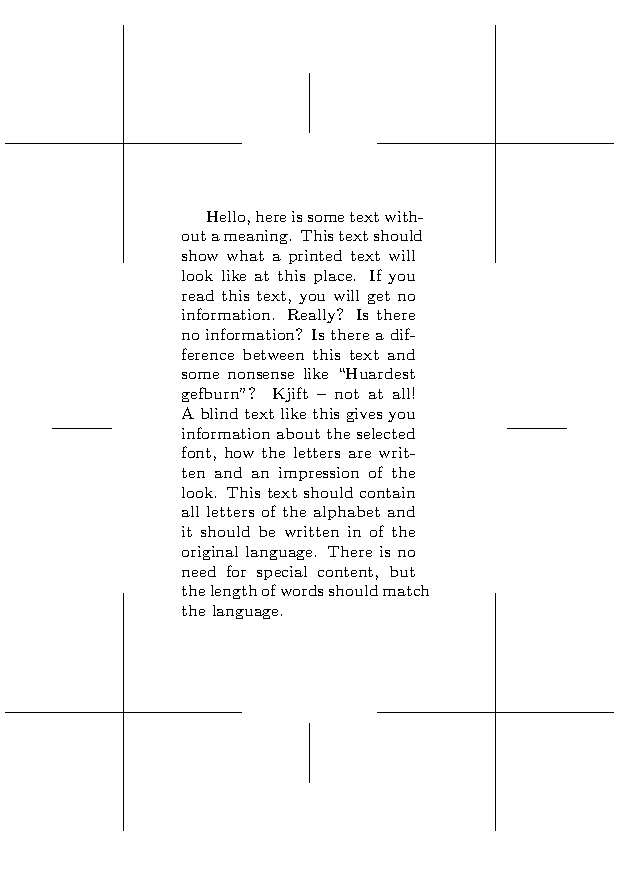
\includegraphics[page=1,scale=0.5]{trims-example}}
  \qquad\qquad
  \subbottom[\cs{trimLmarks}]{\includegraphics[page=2,scale=0.5]{trims-example}}
  \\%
  \subbottom[\cs{trimFrame}]{\includegraphics[page=3,scale=0.5]{trims-example}}
  \qquad\qquad
  \subbottom[\cs{quarkmarks}]{\includegraphics[page=4,scale=0.5]{trims-example}}
  \else%
  \texttt{examples only inserted in pdf-mode, now we can write and
    work in DVI-mode, /daleif}
  \fi%
  \caption{The four trimmark types}
  \label{fig:trimmarks}
\end{figure}





\section{Sheet numbering}

    One purpose of trim marks is to show a printer where the stock
should be trimmed. In this application it can be useful to also note the
sheet number on each page, where the sheet number is 1 for the first page 
and increases by 1 for each page thereafter. The sheet number is independent
of the page number.

\begin{syntax}
\Icn{sheetsequence} \\
\cmd{\thesheetsequence} \\
\end{syntax}
\glossary(sheetsequence)%
  {\Pcn{sheetsequence}}%
  {Counter for sheets (similar to \Pcn{page} for pages).}
\glossary(thesheetsequence)%
  {\cs{thesheetsequence}}%
  {Typesets the current sheet sequence number.}
The macro \cmd{\thesheetsequence} typesets the current sheet sequence number
and is analogous to the \cmd{\thepage} macro.

\begin{syntax}
\Icn{lastsheet} \\
\Icn{lastpage} \\
\end{syntax}
\glossary(lastsheet)%
  {\Pcn{lastsheet}}%
  {Counter holding the number of sheets processed during the \emph{previous}
   \ltx\ run.}
\glossary(lastpage)%
  {\Pcn{lastpage}}%
  {Counter holding the number of the last page processed during the \emph{previous}
   \ltx\ run.}
The counter \Icn{lastsheet} holds the number of sheets processed during
the \emph{previous} run of LaTeX. Similarly, the counter \Icn{lastpage}
holds the number of the last page processed during the previous run.
Note that the last page number is not necessarily the same as the last
sheet number. For example: \\
\textit{In this document this is 
        sheet \thesheetsequence\ of \thelastsheet\ sheets, 
        and page \thepage\ of \thelastpage.}

The previous sentence was the result of processing the following
code 
\begin{lcode}
\textit{In this document this is 
        sheet \thesheetsequence\ of \thelastsheet\ sheets, 
        and page \thepage\ of \thelastpage.}
\end{lcode}

    You may wish to use the sheet and/or page numbers as part of some
trim marks. The following will note the sheet numbers above the page.
\begin{lcode}
\newcommand*{\trimseqpage}{%
  \begin{picture}(0,0)
    \unitlength 1mm
    \put(0,2){\makebox(0,0)[b]{Sheet: \thesheetsequence\ of \thelastsheet}}
  \end{picture}}
\let\tmarktm\trimseqpage
\end{lcode}

\section{Gatherings or signatures}

    Sometimes publishers request that they be supplied with a total number of
pages that meet their planned \emph{gatherings}\index{gathering}.\footnote{There
was a thread on \ctt, \textit{pagenumber mod 4?} about this in 2008.}
 For instance
a gathering may consist of 8 leaves, and as there are two pages to a leaf this
is equivalent to 16 pages. To meet this particular requirement there must be 
a total of $8N$ leaves, or equivalently $16N$ pages, where $N$ will be 
the number of gatherings.

\begin{syntax}
\cmd{\leavespergathering}\marg{num} \\
\end{syntax}
\glossary(leavespergathering)%
  {\cs{leavespergathering}\marg{num}}%
  {Ensure that the correct number of pages are output to make up gatherings 
   of \meta{num} leaves each.}
The command \cmd{\leavespergathering} ensures that there will be exactly the
right number of pages output to make a complete set of gatherings of \meta{num}
leaves (2\meta{num} pages) each --- if necessary  blank pages will be output 
at the end to make up the correct tally. If \meta{num} is less than two (the default)
then no additional pages will be output.


\section{Time}

\begin{syntax}
\cmd{\printtime} \cmd{\printtime*} \\
\cmd{\hmpunct} \cmd{\amname} \cmd{\pmname} \\
\end{syntax}
\glossary(printtime)%
  {\cs{printtime}}%
  {Prints the time of day using a 24 hour clock.}
\glossary(printtime*)%
  {\cs{printtime*}}%
  {Prints the time of day using a 12 hour clock.}
\glossary(hmpunct)%
  {\cs{hmpunct}}%
  {Punctuation between hours and minutes in \cs{printtime} (default :)}
\glossary(amname)%
  {\cs{amname}}%
  {Abbreviation for ante meridiem used in \cs{printtime*} (default am)}
\glossary(pmname)%
  {\cs{pmname}}%
  {Abbreviation for post meridiem used in \cs{printtime*} (default am)}

The \cmd{\printtime} command\footnote{I based the code on a similar macro
in \btitle{\tx\ for the Impatient}~\cite{IMPATIENT}.} 
prints the time of day when the document is 
processed using the 24 hour clock while \cmd{\printtime*} uses a 12
hour clock. For example, the effect of the 
next piece of code is shown below.
\begin{lcode}
This document was processed on: \today\ at \printtime\ (\printtime*).
\end{lcode}
This document was processed on: \today\ at \printtime\ (\printtime*).

    The punctuation between the hours and minutes is \cmd{\hmpunct} which
defaults to a colon (:). The macros \cmd{\amname} and \cmd{\pmnane} hold 
the abbreviations for \textit{ante meridiem} and \textit{post meridiem}, 
respecitively; the defaults are `\amname' and `\pmname'. 

    According to the \btitle{Chicago Manual of Style}~\cite{CMS} there 
should be no punctuation between the hours and minutes in the 24 hour system.
For the 12 hour system it recommends that small caps be used for the
divisions of the day (e.g., \textsc{a.m.} and \textsc{p.m.}) and also
that the American practice is to use a colon as the separator between
hours and minutes whereas the English practice is to use a period (known
to the English as a `full stop'). I don't know what the traditions are
in other orthographies.

    The \cmd{\quarkmarks} declaration uses \cmd{\printtime}, so be careful
if you change it.

    Nicola Talbot's \Lpack{datetime} package~\cite{DATETIME} provides
a much more comprehensive collection of styles for printing the time;
also for dates.

\section{Page breaks before lists}

   A sentence or two may be used to introduce a list (e.g., \Ie{itemize})
and it can be annoying if there is a page break between the introductory words
and the first item.
\begin{syntax}
\cmd{\noprelistbreak} \\
\end{syntax}
\glossary(noprelistbreak)%
  {\cs{noprelistbreak}}%
  {Putting this immediately before an \Pe{itemize} (or \Pe{enumerate}, or \ldots) 
   environment should prevent a pagebreak.}

Putting \cmd{\noprelistbreak} immediately before the \verb?\begin{itemize}?
should prevent a page break. Ideally, there should be no blank lines
between the end of the introduction and the start of the list. 

\section{Changing counters}

    This is effectively a bundling of the \Lpack{chngcntr} 
package~\cite{CHNGCNTR}.

\begin{syntax}
\cmd{\newcounter}\marg{ctr}\oarg{within} \\
\cmd{\thectr} \\
\end{syntax}
\glossary(newcounter)%
  {\cs{newcounter}\marg{ctr}\oarg{within}}%
  {Creates a new counter \Pcn{ctr}, optionally reset when counter \Pcn{within}
   changes.}
\glossary(thectr)%
  {\cs{thectr}}%
  {Typesets the value of the counter \Pcn{ctr}.}
    In \ltx\ a new counter called, say \Pcn{ctr}, is created by the 
\cmd{\newcounter} command as \verb?\newcounter{ctr}?. 
If the optional \meta{within}
argument is given, the counter \Pcn{ctr} is reset to zero each time the 
counter called \Pcn{within} is changed; the \Pcn{within} counter 
must exist before it is used as the optional argument. The command 
\verb?\thectr? typesets the value
of the counter \Pcn{ctr}. This is automatically defined for you by the 
\cmd{\newcounter} command to typeset arabic numerals.

\begin{syntax}
\cmd{\counterwithin}\marg{ctr}\marg{within} \\
\cmd{\counterwithin*}\marg{ctr}\marg{within} \\
\end{syntax}
\glossary(counterwithin)%
  {\cs{counterwithin}\marg{ctr}\marg{within}}%
  {Makes the counter \Pcn{ctr} (created via \cs{newcounter}) act as though 
   it had been initially defined to be reset by counter \Pcn{within}.
   It also redefines \cs{thectr} to include \cs{thewithin}.}
\glossary(counterwithin*)%
  {\cs{counterwithin*}\marg{ctr}\marg{within}}%
  {Makes the counter \Pcn{ctr} (created via \cs{newcounter}) act as though 
   it had been initially defined to be reset by counter \Pcn{within}, leaving
   the original definition of \cs{thectr}.}
The \cmd{\counterwithin} macro makes a \meta{ctr} that has been initially
defined by \verb?\newcounter{ctr}? act as though it had been defined by
\verb?\newcounter{ctr}[within]?. It also redefines the \cs{thectr} command
to be \verb?\thewithin.\arabic{ctr}?. The starred version of the command
does nothing to the original definition of \cs{thectr}.

\begin{syntax}
\cmd{\counterwithout}\marg{ctr}\marg{within} \\
\cmd{\counterwithout*}\marg{ctr}\marg{within} \\
\end{syntax}
\glossary(counterwithout)%
  {\cs{counterwithout}\marg{ctr}\marg{within}}%
  {Makes the counter \Pcn{ctr} (created via 
   \cs{newcounter}\marg{ctr}\oarg{within}) act as though 
   it had been initially defined via \cs{newcounter}\marg{ctr}.
   It also redefines \cs{thectr} to typeset as arabic numerals.}
\glossary(counterwithout*)%
  {\cs{counterwithout*}\marg{ctr}\marg{within}}%
  {Makes the counter \Pcn{ctr} (created via 
   \cs{newcounter}\marg{ctr}\oarg{within}) act as though 
   it had been initially defined via \cs{newcounter}\marg{ctr},
   leaving the original definition of \cs{thectr}.}
The \cmd{\counterwithout} macro makes the \Pcn{ctr} counter that has been 
initially
defined by \verb?\newcounter{ctr}[within]? act as though it had been defined by
\verb?\newcounter{ctr}?. It also redefines the \cs{thectr} command
to be \verb?\arabic{ctr}?. The starred version of the command
does nothing to the original definition of \verb?\thectr?.

    Any number of \verb?\counterwithin{ctr}{...}? and \verb?\counterwithout{ctr}{...}?
commands can be issued for a given counter \Pcn{ctr} if you wish to toggle
between the two styles. The current value of \Pcn{ctr} is unaffected by these
commands. If you want to change the value use \cmd{\setcounter}, and to change
the typesetting style use \cmd{\renewcommand} on \cs{thectr}.

\LMnote{2010/01/30}{Added \cs{letcountercounter}}
\begin{syntax}
  \cmd{\letcountercounter}\marg{counterA}\marg{counterB}\\
  \cmd{\unletcounter}\marg{counterA}\\
\end{syntax}
At times it is handy to `let' one counter act as if it was a
different counter. Say you have two constructions, each with their
own counter A and B, now you want them to cooperate, counting in
unison. This can be done using the \verb?\letcountercounter?.

\cs{letcountercounter}\marg{counterA}\marg{counterB} \cs{let}s 
(make the same) \meta{counterA} to \meta{counterB}. The
original of \meta{counterA} is kept, such that you can unlet it later.

\cs{unletcounter}\marg{counterA} restores \meta{counterA} to its un\cs{let}
condition.

This feature can be quite handy. Say for instance you want figures and
tables to counter within the same counter (say table), then we need
each change to the \verb?figure? counter to actually act on the
\verb?table? counter. \verb?\letcountercounter{figure}{table}? solves
the problem.



\section{New new and provide commands}

\begin{syntax}
\cmd{\newloglike}\marg{cmd}\marg{string} \\
\cmd{\newloglike*}\marg{cmd}\marg{string} \\
\end{syntax}
\glossary(newloglike)%
  {\cs{newloglike}\marg{cmd}\marg{string}}%
  {Creates a new log-like function command \meta{cmd} typesetting 
   \meta{string}.}
\glossary(newloglike*)%
  {\cs{newloglike}\marg{cmd}\marg{string}}%
  {Creates a new log-like function command \meta{cmd} typesetting 
   \meta{string}, which can take limits.}
The class provides means of creating new math log-like functions. For
example you might want to do
\begin{lcode}
\newloglike{\Ei}{Ei}
\end{lcode}
if you are using the exponential integral function in your work.
The starred version of the command creates a function that takes limits
(like the \cmd{\max} function).

    The \ltx\ kernel defines the \cmd{\providecommand} macro that acts
like \cmd{\newcommand} if the designated macro has not been defined
previously, otherwise it does nothing. The class adds to that limited
repertoire.

\begin{syntax}
\cmd{\provideenvironment}\marg{name}\oarg{numargs}\oarg{optarg}\marg{begindef}\marg{enddef} \\
\cmd{\providelength}\marg{cmd} \\
\cmd{\providecounter}\marg{ctr}\oarg{within} \\
\cmd{\provideloglike}\marg{cmd}\marg{string} \\
\cmd{\provideloglike*}\marg{cmd}\marg{string} \\
\end{syntax}
\glossary(provideenvironment)%
  {\cs{provideenvironment}\marg{name}\oarg{numarks}\oarg{optarg}\marg{begindef}\marg{enddef}}%
  {A `provide' version of \cs{(re)newenvironment}.}
\glossary(providelength)%
  {\cs{providelength}\marg{cmd}}%
  {A `provide' version of \cs{newlength}.}
\glossary(providecounter)%
  {\cs{providecounter}\marg{ctr}\oarg{within}}%
  {A `provide' version of \cs{newcounter}.}
\glossary(provideloglike)%
  {\cs{provideloglike}\marg{cmd}\marg{string}}%
  {A `provide' version of \cs{newloglike}.}
\glossary(provideloglike*)%
  {\cs{provideloglike*}\marg{cmd}\marg{string}}%
  {A `provide' version of \cs{newloglike*}.}
    The macros \cmd{\provideenvironment}, \cmd{\providelength}
and \cmd{\providecounter} take the same arguments as their \verb?\new...?
counterparts. If the environment, length or counter has not been defined
then it is defined accordingly, otherwise the macros do nothing except
produce a warning message for information purposes.

   The \cmd{\provideloglike} commands are for math log-like functions,
but they do not produce any warning messages.

\section{Changing macros} \label{sec:addtodef}

     Commands are provided for extending simple macro 
definitions.\index{extend a macro}\index{add to a macro}

\begin{syntax}
\cmd{\addtodef}\marg{macro}\marg{prepend}\marg{append} \\
\cmd{\addtoiargdef}\marg{macro}\marg{prepend}\marg{append} \\
\end{syntax}
\glossary(addtodef)%
  {\cs{addtodef}\marg{macro}\marg{prepend}\marg{append}}%
  {Inserts \meta{prepend} at the start of the current definition of 
   \meta{macro} and \meta{append} at the end, treating the result
   as if it had been defined by \cs{renewcommand}.}
\glossary(addtoiargdef)%
  {\cs{addtoiargdef}\marg{macro}\marg{prepend}\marg{append}}%
  {Inserts \meta{prepend} at the start of the current definition of 
   \meta{macro} (which takes a single argument) and \meta{append} at the 
    end, treating the result as if it had been defined by \cs{renewcommand}.}
The macro \cmd{\addtodef} inserts \meta{prepend} at the start of the
current definition of \meta{macro} and puts \meta{append} at the end,
where \meta{macro} is the name of a macro (including the backslash) which 
takes no arguments. The \cmd{\addtoiargdef} macro is similar except that
\meta{macro} is the name of a macro that takes one argument.

 For example the following are two equivalent
definitions of \verb?\mymacro?:
\begin{lcode}
\newcommand{\mymacro}[1]{#1 is a violinist in spite of being tone deaf}
\end{lcode}
and
\begin{lcode}
\newcommand{\mymacro}[1]{#1 is a violinist}
\addtoiargdef{\mymacro}{}{ in spite of being tone deaf}
\end{lcode}

    The \cmd{\addtoiargdef} (and \cmd{\addtodef}) commands
can be applied several times to the same \meta{macro}. Revising the
previous example we could have
\begin{lcode}
\newcommand{\mymacro}[1]{#1 is a violinist}
\addtoiargdef{\mymacro}{Although somewhat elderly, }%
                       { in spite of being tone deaf}
\addtoiargdef{\mymacro}{}{ and a bagpiper}
\end{lcode}
which is equivalent to
\begin{lcode}
\newcommand{\mymacro}[1]{%
  Although somewhat elderly, #1 is a violinist
  in spite of being tone deaf and a bagpiper}
\end{lcode}

The \meta{prepend} and \meta{append} arguments may include \ltx\ code, 
as shown in this extract from the class code:
\begin{lcode}
\addtoiargdef{\date}{}{%
  \begingroup
    \renewcommand{\thanks}[1]{}
    \renewcommand{\thanksmark}[1]{}
    \renewcommand{\thanksgap}[1]{}
    \protected@xdef\thedate{#1}
  \endgroup}
\end{lcode}
Note that in the case of \cmd{\addtoiargdef} an argument can also refer
to the original argument of the \meta{macro}.

\begin{syntax}
\cmd{\addtodef*}\marg{macro}\marg{prepend}\marg{append} \\
\cmd{\addtoiargdef*}\marg{macro}\marg{prepend}\marg{append} \\
\end{syntax}
\glossary(addtodef*)%
  {\cs{addtodef*}\marg{macro}\marg{prepend}\marg{append}}%
  {Inserts \meta{prepend} at the start of the current definition of 
   \meta{macro} and \meta{append} at the end, treating the result as if it had
   been defined by \cs{renewcommand*}.}
\glossary(addtoiargdef*)%
  {\cs{addtoiargdef*}\marg{macro}\marg{prepend}\marg{append}}%
  {Inserts \meta{prepend} at the start of the current definition of 
   \meta{macro} (which takes a single argument) and \meta{append} at the 
   end, treating the result as if it had been defined by \cs{renewcommand*}.}
These starred versions are for use when the original \meta{macro}
was defined via \cmd{\newcommand*}. Using the starred versions is
like using \cmd{\renewcommand*} and the unstarred versions are like
having used \cmd{\renewcommand}. It is the version (starred or unstarred)
of a sequence of \verb?\addto...? commands that counts when determining whether
the equivalent \verb?\renew...? is treated as starred or unstarred.

    The \verb?\addto...? macros cannot be used to delete any code from 
\meta{macro} nor to add anything except at the start and end. Also,
in general, they cannot be used to change the definition of a macro that
takes an optional argument, or a starred macro.

\begin{syntax}
\cmd{\patchcommand}\marg{macro}\marg{start-code}\marg{end-code} \\
\end{syntax}
\glossary(patchcommand)%
  {\cs{patchcommand}\marg{macro}\marg{start-code}\marg{end-code}}%
  {Inserts \meta{start-code} before the current definition of the 
   \meta{macro} and \marg{end-code} at the end of the current definition.}%

The \cmd{\patchcommand} is from the late 
Michael Downes'\index{Downes, Michael}
\Lpack{patchcmd} package~\cite{PATCHCMD}. 
It inserts the \meta{start-code} at 
the start of the current definition of the macro \meta{macro},
and inserts \meta{end-code} at the end of its current definition.
The \meta{macro} can have zero to nine parameters. If \meta{macro}
uses \cmd{\futurelet} (e.g., it is a starred command or takes an
optional argument) only \meta{start-code} is useful --- 
\meta{end-code} must be empty otherwise things get messed up. If
\meta{macro} has any delimited arguments then \cmd{\patchcommand}
cannot be used.

\section{String arguments}

    In the code for the class I have sometimes used macro arguments
that consist of a `string', like the \texttt{*} arguments in the page layout
macros (e.g., \cmd{\settypeblocksize}), or the \texttt{flushleft}, 
\texttt{center} and \texttt{flushright} strings for the 
\cmd{\makeheadposition} macro.

\begin{syntax}
\cmd{\nametest}\marg{str1}\marg{str2} \\
\piif{ifsamename} \\
\end{syntax}
\glossary(nametest)%
  {\cs{nametest}\marg{str1}\marg{str2}}%
  {Sets \cs{ifsamename} \ptrue\ if \meta{str1} is the same as \meta{str2},
  otherwise \pfalse.}
\glossary(ifsamename)%
  {\cs{ifsamename}}%
  {Result from \cs{nametest}.}
The macro \cmd{\nametest} takes two strings 
as the arguments \meta{str1} and \meta{str2}. It sets \piif{ifsamename}
\ptrue\ if \meta{str1} is the same as \meta{str2}, otherwise it sets
\piif{ifsamename} \pfalse. For the purposes of \cmd{\nametest}, a string is a
sequence of characters which may include spaces and may include
the \verb?\? backslash character; strings are equal if and only if their
character sequences are identical.

    Typically, I have used it within macros for checking on argument
values. For example:
\begin{lcode}
\newcommand{\amacro}[1]{%
  \nametest{#1}{green}
  \ifsamename
%    code for green
  \fi
  \nametest{#1}{red}
  \ifsamename
%    code for red
  \fi
  ...
}
\end{lcode}

\section{Odd/even page checking}

It is difficult to check robustly if the current page is odd or even
but the class does provide a robust method based on writing out a
label and then checking the page reference for the label. This
requires at least two \ltx\ runs to stabilise. This has been extracted
from the original \Lpack{chngpage} package (which is no longer
available). (The class code and \Lpack{chngpage} code is similar but
not identical. There is a later package,
\Lpack{changepage}~\cite{CHANGEPAGE} which contains code that is
identical to the class.)


\begin{syntax}
\cmd{\checkoddpage} \\
\piif{ifoddpage} \\
\cmd{\strictpagecheck} \cmd{\easypagecheck} \\
\end{syntax}
\glossary(checkoddpage)%
  {\cs{checkoddpage}}%
  {Sets \cs{ifoddpage} \ptrue\ if called on an odd-numbered page, otherwise
   \pfalse.}
\glossary(ifoddpage)%
  {\cs{ifoddpage}}%
  {Result of \cs{checkoddpage}.}
\glossary(strictpagecheck)%
  {\cs{strictpagecheck}}%
  {\cs{checkoddpage} will use an accurate but time and space consuming method
   for checking for an  odd page number.}
\glossary(easypagecheck)%
  {\cs{easypagecheck}}%
  {\cs{checkoddpage} will use a possibly inaccurate but fast method
   for checking for an  odd page number.}
The macro \cmd{\checkoddpage} sets \piif{ifoddpage} to \ptrue\ if the current
page number 
is odd, otherwise it sets it to \pfalse\ (the page number is even). The robust
checking method involves writing and reading labels, which is what is done
after the command \cmd{\strictpagecheck} is issued; it may take more than 
one run before everything settles down. The simple method 
is just
to check the current page number which, because of TeX's asynchronous page
breaking algorithm, may not correspond to the actual page number where the
\cmd{\checkoddpage} command was issued. The simple, but faster, page checking
method is used after the \cmd{\easypagecheck} command is issued.

\begin{syntax}
\cmd{\cplabel} \\
\end{syntax}
\glossary(cplabel)%
  {\cs{cplabel}}%
  {Prefix for labels used by \cs{checkoddpage} odd/even page checking.}
When strict page checking is used the labels consist of a number preceded
by the value of \cmd{\cplabel}, whose default definition is \verb?^_? (e.g.,
a label may consist of the characters \verb?^_21?). If this
might clash with any of your labels, change \cmd{\cplabel} with 
\cmd{\renewcommand}, but
the definition of \cmd{\cplabel} must be constant for any given document.

\section{Moving to another page} \label{sec:moving}

   Standard \ltx\ provides the \cmd{\newpage}, \cmd{\clearpage}
and \cmd{\cleardoublepage} commands for discontinuing the current 
page and starting a new one. The following is a bundling of the
\Lpack{nextpage} package~\cite{NEXTPAGE}.

\begin{syntax}
\cmd{\needspace}\marg{length} \\
\end{syntax}
\glossary(needspace)%
  {\cs{needspace}\marg{length}}%
  {Starts a new page, leaving the current page short, unless there is 
   estimated \meta{length} vertical space left on the current page.}
This macro decides if there is \meta{length} space at the bottom of the 
current page. If there is, it does nothing, otherwise it starts a new page.
This is useful if \meta{length} amount of material is to be kept together
on one page. The \cmd{\needspace} macro 
depends on penalties for deciding what to do which means that the reserved
space is an approximation. However, except for the odd occasion, the
macro gives adequate results. 

\begin{syntax}
\cmd{\Needspace}\marg{length} \\
\cmd{\Needspace*}\marg{length} \\
\end{syntax}
\glossary(Needspace)%
  {\cs{Needspace}\marg{length}}%
  {Starts a new page, leaving the current page short, unless there is 
   actually at least \meta{length} vertical space left on the current page. }
\glossary(Needspace*)%
  {\cs{Needspace*}\marg{length}}%
  {Starts a new page, leaving the current page short unless \cs{flushbottom} 
   is in effect, unless there is 
   actually at least \meta{length} vertical space left on the current page.}
    Like \cmd{\needspace}, the \cmd{\Needspace} macro checks if there is
\meta{length} space at the bottom of the current page and if there is not
it starts a new page. The command should only be used between paragraphs;
indeed, the first thing it does is to call \cs{par}. The \cmd{\Needspace}
command checks for the actual space left on the page and is more exacting
than \cmd{\needspace}.

    If either \cmd{\needspace} or \cmd{\Needspace} produce a short page it
will be ragged bottom even if \cmd{\flushbottom} is in effect. With
the starred \cmd{\Needspace*} version, short pages will be flush bottom
if \cmd{\flushbottom} is in effect and will be ragged bottom
when \cmd{\raggedbottom} is in effect.

    Generally speaking, use \cmd{\needspace} in preference to \cmd{\Needspace}
unless it gives a bad break or the pages must be flush bottom.


\begin{syntax}
\cmd{\movetoevenpage}\oarg{text} \\
\cmd{\cleartoevenpage}\oarg{text} \\
\end{syntax}
\glossary(movetoevenpage)%
  {\cs{movetoevenpage}\oarg{text}}%
  {Stops the current page to start typesetting on the next even page.
   The optional \meta{text} is put on the skipped page (if there is one).}
The \cmd{\movetoevenpage} stops the current page and starts typesetting on the
next even numbered page. The \verb?\clear...? version flushes out all 
floats\index{float} before
going to the next even page. The optional \meta{text} is put on the skipped
page (if there is one).

\begin{syntax}
\cmd{\movetooddpage}\oarg{text} \\
\cmd{\cleartooddpage}\oarg{text} \\
\end{syntax}
\glossary(movetooddpage)%
  {\cs{movetooddpage}\oarg{text}}%
  {Stops the current page to start typesetting on the next odd page.
   The optional \meta{text} is put on the skipped page (if there is one).}
\glossary(cleartoevenpage)%
  {\cs{cleartooddpage}\oarg{text}}%
  {Flushes any pending floats to then start typesetting on the next odd page.
   The optional \meta{text} is put on the skipped page (if there is one).}
These macros are similar to the \verb?\...evenpage? ones except that they jump
to the next odd numbered page.

    A likely example for the optional \meta{text} argument is
\begin{lcode}
\cleartooddpage[\vspace*{\fill}THIS PAGE LEFT BLANK\vspace*{\fill}]
\end{lcode}
which will put `THIS PAGE LEFT BLANK' in the centre of any
potential skipped (empty) even numbered page.

\begin{syntax}
\cmd{\cleartorecto} \cmd{\cleartoverso} \\
\end{syntax}
\glossary(cleartorecto)%
  {\cs{cleartorecto}}%
  {Simpler form of \cs{cleartooddpage}.}
\glossary(cleartoverso)%
  {\cs{cleartoverso}}%
  {Simpler form of \cs{cleartoevenpage}.}
These are slightly simpler forms\footnote{Perhaps more robust.} of
\cmd{\cleartooddpage} and \cmd{\cleartoevenpage}. For example, if you wanted
the \toc\ to start on a verso page, like in 
\btitle{The TeXbook} \cite{TEXBOOK}, then do this:
\begin{lcode}
\cleartoverso
\tableofcontents
\end{lcode}

\section{Number formatting}

    Several methods are provided for formatting numbers\index{number}. 
Two classes of number representations\indextwo{number}{representation} 
are catered for. 
A `numeric number'\indextwo{numeric}{number} is typeset using arabic 
digits and a `named number'\indextwo{named}{number} is typeset using
words.

    The argument to the number formatting macros is a `number'\index{number}, 
essentially something that resolves to a series of arabic digits. Typical
arguments might be:
\begin{itemize}
\item Some digits, e.g., \verb?\ordinal{123} ->? 
      \ordinal{123} 
\item A macro expanding to digits, e.g., \verb?\def\temp{3}\ordinal{\temp} ->? 
      \begingroup\def\temp{3}\ordinal{\temp}\endgroup % \\

%      Or even, for example, \verb?\ordinal{\pageref{chap:numf}} ->? 
%      \ordinal{\pageref{chap:numf}}
\item The value of a counter, e.g., \verb?\ordinal{\value{page}} ->? 
      \ordinal{\value{page}} 
\item The arabic representation of a counter, e.g., \verb?\ordinal{\thepage} ->? 
      \ordinal{\thepage} 

However, if the representation of a counter is not completely in arabic 
digits, such as \verb?\thesection? which here prints as \thesection, it will 
produce odd errors or peculiar results if it is used as the argument.
For instance: \\
\verb?\ordinal{\thesection} ->? \ordinal{\thesection}

\end{itemize}

\subsection{Numeric numbers}
\indextwo{numeric}{number}

\begin{syntax}
\cmd{\cardinal}\marg{number} \\
\cmd{\fcardinal}\marg{number} \\
\cmd{\fnumbersep} \\
\end{syntax}
\glossary(cardinal)%
  {\cs{cardinal}\marg{number}}%
  {Typesets \marg{number} as a cardinal number.}
\glossary(fcardinal)%
  {\cs{fcardinal}\marg{number}}%
  {Typesets \marg{number} as a cardinal number, with \cs{fnumbersep} between
   each triple of digits.}
\glossary(fnumbersep)%
  {\cs{fnumbersep}}%
  {Separator between digit triples in numbers.}
The macro \cmd{\fcardinal} prints its \meta{number} argument formatted using
\cmd{\fnumbersep} between each triple of digits. The default definition
of \cmd{\fnumbersep} is:
\begin{lcode}
\newcommand{\fnumbersep}{,}
\end{lcode}

    Here are some examples: \\
\verb?\fcardinal{12} ->? \fcardinal{12} \\
\verb?\fcardinal{1234} ->? \fcardinal{1234} \\
\verb?\fcardinal{1234567} ->? \fcardinal{1234567} \\
\verb?\renewcommand*{\fnumbersep}{\:}\fcardinal{12345678} ->?
\renewcommand*{\fnumbersep}{\:}\fcardinal{12345678} \\
\verb?\renewcommand*{\fnumbersep}{,\:}?
\renewcommand*{\fnumbersep}{,\:}

    The \cmd{\cardinal} macro is like \cmd{\fcardinal} except that there
is no separation between any of the digits.

\begin{syntax}
\cmd{\ordinal}\marg{number} \\
\cmd{\fordinal}\marg{number} \\
\cmd{\ordscript}\marg{chars} \\
\end{syntax}
\glossary(ordinal)%
  {\cs{ordinal}\marg{number}}%
  {Typesets \marg{number} as an ordinal number.}
\glossary(fordinal)%
  {\cs{fordinal}\marg{number}}%
  {Typesets \marg{number} as an ordinal number, with \cs{fnumbersep} between
   each triple of digits.}
\glossary(ordscript)%
  {\cs{ordscript}\marg{chars}}%
  {Typesets the ordinal characters \meta{chars}.}

The \cmd{\fordinal} macro typesets its \meta{number} argument as a formatted
ordinal, using \cmd{\fnumbersep} as the separator. The macro \cmd{\ordinal}
is similar except that there is no separation between any of the digits.

    Some examples are: \\
\verb?\fordinal{3} ->? \fordinal{3} \\
\verb?\fordinal{12341} ->? \fordinal{12341} \\
\verb?\renewcommand{\ordscript}[1]{\textsuperscript{#1}}? \\
\verb?\fordinal{1234567} ->?
  \renewcommand{\ordscript}[1]{\textsuperscript{#1}}\fordinal{1234567} \\
\verb?\ordinal{1234567} ->? \ordinal{1234567} \\
\verb?This is the \ordinal{\value{chapter}} chapter. ->? 
  This is the \ordinal{\value{chapter}} chapter.


    The characters denoting the ordinal (ordination?) are typeset as 
the argument of \cmd{\ordscript}, whose default definition is:
\begin{lcode}
\newcommand{\ordscript}[1]{#1}
\end{lcode}
As the above examples show, this can be changed to give a different
appearance.

\begin{syntax}
\cmd{\nthstring} \cmd{\iststring} \cmd{\iindstring} \cmd{\iiirdstring} \\
\end{syntax}
\glossary(nthstring)%
  {\cs{nthstring}}%
  {Ordinal characters for `th', e.g., as in 6th.}
\glossary(iststring)%
  {\cs{iststring}}%
  {Ordinal characters for `st', e.g., as in 1st.}
\glossary(iindstring)%
  {\cs{iindstring}}%
  {Ordinal characters for `nd', e.g., as in 2nd.}
\glossary(iiirdstring)%
  {\cs{iiirdstring}}%
  {Ordinal characters for `rd', e.g., as in 3rd.}
The ordinal characters are the values of the macros \cmd{\nthstring}
(default: th) for most ordinals, \cmd{\iststring} (default: st) for
ordinals ending in 1 like \ordinal{21}, \cmd{\iindstring} (default: nd)
for ordinals like \ordinal{22}, and \cmd{\iiirdstring} (default: rd)
for ordinals like \ordinal{23}.


\subsection{Named numbers}
\indextwo{named}{number}


\begin{syntax}
\cmd{\numtoname}\marg{number} \\
\cmd{\numtoName}\marg{number} \\
\cmd{\NumToName}\marg{number} \\
\end{syntax}
\glossary(numtoname)%
  {\cs{numtoname}\marg{number}}%
  {Typesets \meta{number} as a cardinal using lowercase words.}
\glossary(numtoName)%
  {\cs{numtoName}\marg{number}}%
  {Typesets \meta{number} as a cardinal using lowercase words, but uppercase for the initial
   letter of the first word.}
\glossary(NumtoName)%
  {\cs{NumtoName}\marg{number}}%
  {Typesets \meta{number} as a cardinal using lowercase words, but uppercase for the initial
   letter of each word.}
The macro \cmd{\numtoname} typesets its \meta{number} argument using 
lowercase words. The other two macros are similar, except that 
\cmd{\numtoName} uses uppercase for the initial letter of the first word and
\cmd{\NumToName} uses uppercase for the initial letters of all the words.

    As examples: \\
\verb?\numtoname{12345} ->? \numtoname{12345} \\
\verb?\numtoName{12345} ->? \numtoName{12345} \\
\verb?\NumToName{12345} ->? \NumToName{12345} \\
\begin{egsource}{eg:minnum}
The minimum number in TeX is \numtoname{-2147483647}
(i.e., \fcardinal{-2147483647})
\end{egsource}
\begin{egresult}[\tx's minimum number in words (English style)]{eg:minnum}
  The minimum number in TeX is \numtoname{-2147483647} 
  (i.e., \fcardinal{-2147483647})
\end{egresult}

\begin{syntax}
\cmd{\ordinaltoname}\marg{number} \\
\cmd{\ordinaltoName}\marg{number} \\
\cmd{\OrdinalToName}\marg{number} \\
\end{syntax}
\glossary(ordinaltoname)%
  {\cs{ordinaltoname}\marg{number}}%
  {Typeset \meta{number} as an ordinal using lowercase words.}
\glossary(ordinaltoName)%
  {\cs{ordinaltoName}\marg{number}}%
  {Typeset \meta{number} as an ordinal using lowercase words, but uppercase the
   initial letter of the first word.}
\glossary(OrdinaltoName)%
  {\cs{OrdinaltoName}\marg{number}}%
  {Typeset \meta{number} as an ordinal using lowercase words, but uppercase the
   initial letter of each word.}
These three macros are similar to \cmd{\numtoname}, etc., except that they
typeset the argument as a wordy ordinal.

    For example: \\
\verb?This is the \ordinaltoname{\value{chapter}} chapter. ->? 
  This is the \ordinaltoname{\value{chapter}} chapter.

\begin{syntax}
\cmd{\namenumberand} \cmd{\namenumbercomma} \cmd{\tensunitsep} \\
\end{syntax}
\glossary(namenumberand)%
  {\cs{namenumberand}}%
  {The conjunction in named numbers, default ` and '.}
\glossary(namenumbercomma)%
  {\cs{namenumbercomma}}%
  {The `comma' in named numbers, default `, '.}
\glossary(tensunitsep)%
  {\cs{tensunitsep}}%
  {The separator/conjoiner between tens and units in named numbers, default `-'.}
By default some punctuation and conjunctions are used in the representation
of named numbers. According to both American and English practice, a hyphen
should be inserted between a `tens' name (e.g., fifty) and a following 
unit name (e.g., two). This is represented by the value of \cmd{\tensunitsep}.
English practice, but not American, is to include commas (the value of
\cmd{\namenumbercomma}) and conjunctions (the value of \cmd{\namenumberand})
in strategic positions in the typesetting. These macros are initially
defined as:
\begin{lcode}
\newcommand*{\namenumberand}{ and }
\newcommand*{\namenumbercomma}{, }
\newcommand*{\tensunitsep}{-}
\end{lcode}
The next example shows how to achieve American typesetting.
\begin{egsource}{eg:maxnum}
\renewcommand*{\namenumberand}{ }
\renewcommand*{\namenumbercomma}{ }
The maximum number in TeX is \numtoname{2147483647} 
(i.e., \cardinal{2147483647}).
\end{egsource}
\begin{egresult}[\tx's maximum number in words (American style)]{eg:maxnum}
\renewcommand*{\namenumberand}{ }\renewcommand*{\namenumbercomma}{ }%
The maximum number in TeX is \numtoname{2147483647} 
(i.e., \cardinal{2147483647}). 
\end{egresult}
\renewcommand*{\namenumberand}{ and }
\renewcommand*{\namenumbercomma}{, }

\begin{syntax}
\cmd{\minusname} \cmd{\lcminusname} \cmd{\ucminusname} \\
\end{syntax}
\glossary(minusname)%
  {\cs{minusname}}%
  {Typeset for `minus' before negative named numbers.}
\glossary(lcminusname)%
  {\cs{lcminusname}}%
  {Lowercase `minus' name, default `minus'.}
\glossary(ucminusname)%
  {\cs{ucminusname}}%
  {Lowercase `minus' name with initial uppercase letter, default `Minus'.}
    When a named number is negative, \cmd{\minusname} is put before the
spelled out number. The definitions of the above three comands are:
\begin{lcode}
\newcommand*{\lcminusname}{minus }
\newcommand*{\ucminusname}{Minus }
\let\minusname\lcminusname
\end{lcode}
which means that `minus' is normally all lowercase. To get `minus'
typeset with an initial uppercase letter simply:
\begin{lcode}
\let\minusname\ucminusname
\end{lcode}

    Only one version of \cmd{\namenumberand} is supplied as I consider that
it is unlikely that `and' would ever be typeset as `And'. If the initial
uppercase is required, renew the macro when appropriate.

    There is a group of macros that hold the names for the numbers. To
typeset named numbers in a language other than English these will have to be
changed as appropriate. You can find them in the class and patch code. 
The actual picking and ordering of the names is done by an internal macro
called \cmd{\n@me@number}. If the ordering is not appropriate for a
particular language, that is the macro to peruse and modify. Be prepared,
though, for the default definitions to be changed in a later release in case
there is a more efficient way of implementing their functions.

    If you want to express numbers that fall outside \tx's range, Edward
Reingold has produced a set of macros that can write out in words any number
within the range $-10^{66} to 10^{66}$, that is, up to a thousand 
vigintillion~\cite{REINGOLD07}.

\subsection{Fractions}

    When typesetting a simple fraction in text there is usually a choice
of two styles, like 3/4 or $\frac{3}{4}$, which do not necessarily look 
as though they fit in with their surroundings. These fractions were
typeset via:
\begin{lcode}
... like 3/4 or $\frac{3}{4}$ ...
\end{lcode}

\begin{syntax}
\cmd{\slashfrac}\marg{top}\marg{bottom} \\
\cmd{\slashfracstyle}\marg{num} \\
\end{syntax}
\glossary(slashfrac)%
  {\cs{slashfrac}\marg{top}\marg{bottom}}%
  {Typesets like \slashfrac{3}{4}, using the \cs{slashfracstyle} font.}
\glossary(slashfracstyle)%
  {\cs{slashfracstyle}\marg{num}}%
  {Typesets \meta{num} in a particular (font, size) style.}
The class provides the \cmd{\slashfrac} command which typesets its
arguments like \slashfrac{3}{4}. Unlike the \cmd{\frac} command which
can only be used in math mode, the \cmd{\slashfrac} command can be
used in text and math modes.

    The \cmd{\slashfrac} macro calls the \cmd{\slashfracstyle} command to
reduce the size of the numbers in the fraction. You can also use
\cmd{\slashfracstyle} by itself.
\begin{egsource}{eg:fractions}
In summary, fractions can be typeset like 3/4 or $\frac{3}{4}$
or \slashfrac{3}{4} or \slashfracstyle{3/4} because several choices
are provided.
\end{egsource}
\begin{egresult}[Varieties of fractions in text]{eg:fractions}
In summary, fractions can be typeset like 3/4 or $\frac{3}{4}$
or \slashfrac{3}{4} or \slashfracstyle{3/4} because several choices
are provided.
\end{egresult}

\begin{syntax}
\cmd{\textsuperscript}\marg{super} \\
\cmd{\textsubscript}\marg{sub} \\
\end{syntax}
\glossary(textsuperscript)%
  {\cs{textsuperscript}\marg{super}}%
  {Typesets \meta{super} as a superscript.}
\glossary(textsubscript)%
  {\cs{textsubscript}\marg{sub}}%
  {Typesets \meta{sub} as a subscript.}
While on the subject of moving numbers up and down, the kernel provides
the \cmd{\textsuperscript} macro for typesetting its argument as though it
is a superscript. The class also provides the \cmd{\textsubscript} macro
for typesetting its argument like a subscript.

\begin{egsource}{eg:textsupsub}
In normal text you can typeset superscripts like H\textsuperscript{+} and 
subscripts like H\textsubscript{2}O without going into math mode.
\end{egsource}
\begin{egresult}[Super- and subscripts in text]{eg:textsupsub}
In normal text you can typeset superscripts like H\textsuperscript{+} and 
subscripts like H\textsubscript{2}O without going into math mode.
\end{egresult}

\section{An array data structure}

   The class includes some macros for supporting the \Ie{patverse}
environment which may be more generally useful. 

\begin{syntax}
\cmd{\newarray}\marg{arrayname}\marg{low}\marg{high} \\
\end{syntax}
\glossary(newarray)%
  {\cs{newarray}\marg{arrayname}\marg{low}\marg{high}}%
  {Defines a new indexed array datastructure called \meta{arrayname}
  with the (integer) index ranging from \meta{low} to \meta{high}.}
 
\cmd{\newarray} defines
the \meta{arrayname} array, where \meta{arrayname} is a name like
\texttt{MyArray}. The lowest and highest array indices are set to
\meta{low} and \meta{high} respectively, where both are integer numbers.

\begin{syntax}
\cmd{\setarrayelement}\marg{arrayname}\marg{index}\marg{text} \\
\cmd{\getarrayelement}\marg{arrayname}\marg{index}\marg{result} \\
\end{syntax}
\glossary(setarrayelement)%
  {\cs{setarrayelement}\marg{arrayname}\marg{index}\marg{text}}%
  {Makes \meta{text} the contents of the \marg{index} location in 
   array \meta{arrayname}.}
\glossary(getarrayelement)%
  {\cs{getarrayelement}\marg{arrayname}\marg{index}\marg{result}}%
  {Sets the parameterless macro \meta{result} to the contents of 
   the \marg{index} location in array \meta{arrayname}.}

The \cmd{\setarrayelement} macro
sets the \meta{index} location in the \meta{arrayname} array to be 
\meta{text}. Conversely, \cmd{\getarrayelement} sets the parameterless
macro \meta{result} to the contents of
the \meta{index} location in the \meta{arrayname} array. 
For example: 
\begin{lcode}
\setarrayelement{MyArray}{23}{$2^{23}$}
\getarrayelement{MyArray}{23}{\result}
\end{lcode}
will result in \verb?\result? being defined as \verb?\def\result{$2^{23}$}?.

\begin{syntax}
\cmd{\checkarrayindex}\marg{arrayname}\marg{index} \\
\piif{ifbounderror} \\
\end{syntax}
\glossary(checkarrayindex)%
  {\cs{checkarrayindex}\marg{arrayname}\marg{index}}%
  {Checks if \meta{index} is a valid index value for the array 
   \meta{arrayname}. Sets \cs{ifbounderror} \ptrue\ if there is a problemn
   otherwise \pfalse.}
\cmd{\checkarrayindex} checks if
\meta{arrayname} is an array and if \meta{index} is a valid index for
the array. If both conditions hold then \piif{ifbounderror} is set
\pfalse, but if either \meta{arrayname} is not an array or, if it is,
\meta{index} is out of range then \piif{ifbounderror} is set \ptrue.

\begin{syntax}
\cmd{\stringtoarray}\marg{arrayname}\marg{string} \\
\cmd{\arraytostring}\marg{arrayname}\marg{result} \\
\end{syntax}
\glossary(stringtoarray)%
  {\cs{stringtoarray}\marg{arrayname}\marg{string}}%
  {Puts each character from \meta{string} sequentially into array 
   \meta{arrayname}, starting at index 1.}
\glossary(arraytostring)%
  {\cs{arraytostring}\marg{arrayname}\marg{result}}%
  {Defines the macro \meta{result} to be the sequence of characters
   in the array \meta{arrayname}.}
The macro \cmd{\stringtoarray} puts each character
from \meta{string} sequentially into the \meta{arrayname} array, starting
at index 1.
The macro \cmd{\arraytostring} assumes
that \meta{arrayname} is an array of characters, and defines the macro
\meta{result} to be that sequence of characters. For example: \\
\begin{lcode}
\stringtoarray{MyArray}{Chars}
\arraytostring{MyArray}{\MyString}
\end{lcode}
is equivalent to 
\begin{lcode}
\def\MyString{Chars}
\end{lcode}

\begin{syntax}
\cmd{\checkifinteger}\marg{num} \\
\piif{ifinteger} \\
\end{syntax}
\glossary(checkifinteger)%
  {\cs{checkifinteger}\marg{num}}%
  {If \meta{num} is an integer and not less than zero, sets \cs{ifinteger}
   \ptrue, otherwise \pfalse.}
The command \cmd{\checkifinteger} ckecks if \meta{num} is an integer 
(not less than zero). If it is then \piif{ifinteger} is set \ptrue, 
otherwise it is set \pfalse.
%
\begin{note}
  Please note that \cmd{\checkifinteger} may only work on simple input.
\end{note}


\section{Checking the processor}

\subsection{Checking for pdfLaTeX}

    Both \ltx\ and \pixpdfltx\ can be run on the same document. \ltx\ produces
a \file{.dvi} file as output, while \pixpdfltx\ can produce either a
\file{.dvi} or a \file{.pdf} file. 
    On modern systems \pixpdfltx\ produces a \file{pdf} file by default.

If you want a \file{dvi} file output use \ltx\ and if you want a
\file{pdf} file use \pdfltx.

\begin{syntax}
\piif{ifpdf} ... \verb?\fi? \\
\end{syntax}
The class provides \piif{ifpdf} which is \ptrue\ when the document is
being processed by \pixpdfltx\ and \pfalse\ otherwise. You can use it like this:
\begin{lcode}
\ifpdf
  code for pdfLaTeX only 
\else
  code for LaTeX only
\fi
\end{lcode}
If there is no \ltx\ specific code then don't write the \verb?\else? part.

\subsection{Checking for etex}

    Modern \ltx\ distributions use \pixetx, which is an extended version
of \tx, as the underlying engine. \pixetx\ provides some more primitives
than \tx, which may be useful, but not everybody has \pixetx\ available.

\begin{syntax}
\piif{ifetex} \\
\end{syntax}
\glossary(ifetex)%
  {\cs{ifetex}}%
  {\ptrue\ if \etx\ is the underlying engine, otherwise \pfalse.}
\piif{ifetex} can be used to determine if \pixetx\ is being used as the
underlying engine; it is analagous to \piif{ifpdf} which tests for
\pixpdfltx. For example:
\begin{lcode}
\ifetex
  %%% code only processible by etex
\else
  \typeout{etex is not available}
\fi
\end{lcode}


\subsection{Checking for XeTeX}

    You have been able to use \cs{ifpdf} to check if \pixpdfltx\ is being used 
to process the document.

\begin{syntax}
\piif{ifxetex} \\
\end{syntax}
\glossary(ifxetex)%
  {\cs{ifxetex}}%
  {\ptrue\ if \xetx\ is being used to process the document.}

In a similar manner you can use \piif{ifxetex} to check if the document
is being processed by \pixxetx.

\begin{syntax}
\cmd{\RequireXeTeX} \\
\end{syntax}
\glossary(RequireXeTeX)%
  {\cs{RequireXeTeX}}%
  {Generates an error if the document is not being processed by \xetx.}
The class also provides \cmd{\RequireXeTeX}, which generates an error if
\pixxetx\ is not being used to process the document.


\section{Leading}

    LaTeX automatically uses different leading\index{leading} for different
font sizes. 
\begin{syntax}
\lnc{\baselineskip} \lnc{\onelineskip} \\
\end{syntax}
\glossary(onelineskip)%
  {\ls{onelineskip}}%
  {Distance between baselines of the document's main font and size.}

At any point in a document the standard LaTeX \lnc{\baselineskip} length
contains the current value of the leading\footnote{This statement ignores
any attempts to stretch the baseline.}. The class provides the length
\lnc{\onelineskip} which contains the initial leading for the normal
font. This value is useful if you are wanting to specify length values
in terms of numbers of lines of text.

\section{Minor space adjustment}

    The kernel provides the \cmd{\,} macro for inserting a thin space in both
text and math mode. There are
other space adjustment commands, such as \pixabang\ for negative thin space, 
and \cmd{\:} and \cmd{\;} for medium
and thick spaces, which can only be used in math mode.

\begin{syntax}
\cmd{\thinspace} \cmd{\medspace} \cmd{\:} \pixabang \\
\end{syntax}
\glossary(thinspace)%
  {\cs{thinspace}}%
  {A thin space (3/18 em).}
\glossary(medspace)%
  {\cs{medspace}}%
  {A medium space (4/18 em).}
\glossary(:)%
  {\cs{:}}%
  {A medium space (4/18 em).}
\glossary(!)%
  {\cs{!}}%
  {A negative thin space (-3/18 em).}
On occasions I have found it useful to be able to tweak spaces in text by some
fixed amount, just as in math mode. The kernel macro \cmd{\thinspace}
specifies a thin space, which is 3/18\,em. 
The class \cmd{\medspace} specifies a medium space of 4/18\,em. 
As mentioned, the kernel macro \cmd{\:} inserts
a medium space in math mode. The class version can be used in both math and
text mode to insert a medium space. Similarly, the class version of 
\pixabang{}
can be used to insert a negative thin space in both text and math mode.

    The math thick space is 5/18\,em. 
To specify this amount of space
in text mode you can combine spacing commands as:
\begin{lcode}
\:\:\!
\end{lcode}
which will result in an overall space of 5/18\,em 
(from $(4 + 4 - 3)/18$).

\begin{comment}
\section{Cross references}\label{sec:xrefthis}  \label{sec:xref}

    LaTeX supplies the \cmd{\ref} and \cmd{\pageref} commands for cross
referencing to a label or a page which has a label on it.

\begin{syntax}
\cmd{\fref}\marg{label} \cmd{\figurerefname} \\
\cmd{\tref}\marg{label} \cmd{\tablerefname} \\
\cmd{\pref}\marg{label} \cmd{\pagerefname} \\
\end{syntax}
 
    The class provides these more particular named references to a figure\index{figure!reference},
table\index{table!reference} or page\index{page!reference}. For example the default definitions of \cmd{\fref} and 
\cmd{\pref} are
\begin{lcode}
\newcommand{\fref}[1]{\figurerefname~\ref{#1}}
\newcommand{\pref}[1]{\pagerefname~\pageref{#1}}
\end{lcode}
and can be used as 
\begin{lcode}
\ldots footnote parameters are shown in~\fref{fig:fn} on~\pref{fig:fn}.
\end{lcode}
which in this document prints as: 
\begin{syntax}
\ldots footnote parameters are shown in~\fref{fig:fn} on~\pref{fig:fn}. \\
\end{syntax}

\begin{syntax}
\cmd{\Pref}\marg{label} \cmd{\partrefname} \\
\cmd{\Cref}\marg{label} \cmd{\chapterrefname} \\
\cmd{\Sref}\marg{label} \cmd{\sectionrefname} \\
\end{syntax}

    Also provided are named references to labelled 
Part (\cmd{\Pref}), 
Chapter (\cmd{\Cref}) and 
sectional (\cmd{\Sref}) divisions.
These are all defined like
\begin{lcode}
\newcommand{\Sref}[1]{\sectionrefname\ref{#1}}
\end{lcode}
with no tie between the name and the \cmd{\ref}. 

    In this document
\begin{lcode}
`In \Cref{chap:misc} there is a section 
(\Sref{sec:xrefthis}) about cross references.' 
\end{lcode}
is typeset as: 
\begin{syntax}
`In \Cref{chap:misc} there is a section 
(\Sref{sec:xrefthis}) about cross references.' \\
\end{syntax}
 
    It can be useful to refer to parts of a document by name rather than
number, as in
\begin{lcode}
The chapter \textit{\titleref{chap:bringhurst}} describes \ldots
\end{lcode}
The chapter \textit{\titleref{chap:bringhurst}} describes \ldots

    There are two packages, \Lpack{nameref}~\cite{NAMEREF} and 
\Lpack{titleref}~\cite{TITLEREF},
 that let you refer to things by name instead of number.

    Name references were added to the class as a consequence of adding
a second optional argument to the sectioning commands. I found
that this broke the \Lpack{nameref} package, and hence the
\Lpack{hyperref} package as well, so they had to be fixed. The change 
also broke Donald Arseneau's \Lpack{titleref} package, and it turned out
that \Lpack{nameref} also clobbered \Lpack{titleref}. The class also
provides titles, like \cmd{\poemtitle}, that are not recognised by
either of the packages. From my viewpoint the most efficient
thing to do was to enable the class itself to provide name 
referencing.

\begin{syntax}
\cmd{\label}\marg{key} \cmd{\ref}\marg{key} \cmd{\pageref}\marg{key} \\
\cmd{\titleref}\marg{key} \\
\cmd{\headnamereftrue} \cmd{\headnamereffalse} \\
\end{syntax}
The macro \cmd{\titleref} is an addition to the usual set of cross referencing
commands. Instead of typesetting a number it typesets the title associated
with the labelled number. This is, of course, only useful if there is an
associated title, such as from a \cmd{\caption} or \cmd{\section} command.
As a bad example:
\begin{lcode}
Labelling for \verb?\titleref? may be applied to:
\begin{enumerate}
\item Chapters, sections, etc.       \label{sec:xref:item1}
...
\item Items in numbered lists, etc. \ldots \label{sec:xref:item3}
\end{enumerate}
Item \ref{sec:xref:item2} in section~\ref{sec:xref} mentions captions
while item \titleref{sec:xref:item3} in the same section 
\textit{\titleref{sec:xref}} lists other things.
\end{lcode}
Labelling for \verb?\titleref? may be applied to:
\begin{enumerate}
\item Chapters, sections, etc.       \label{sec:xref:item1}
\item Captions                       \label{sec:xref:item2}
\item Legends
\item Poem titles
\item Items in numbered lists, etc.  \label{sec:xref:item3}
\end{enumerate}
Item \ref{sec:xref:item2} in section~\ref{sec:xref} mentions captions
while item \titleref{sec:xref:item3} in the same section 
\textit{\titleref{sec:xref}} lists other things.


    As the above example shows, you have to be a little careful in using
\cmd{\titleref}.
Generally speaking, \cmd{\titleref}\marg{key} produces the last named 
thing before the \cmd{\label} that defines the \meta{key}. 

    Chapters, and the lower level sectional divisions, may have three
different title texts --- the main title, the title in the ToC, and a third
in the page header. By default (\cmd{\headnamereffalse}) the ToC title
is produced by \cmd{\titleref}. Following the declaration
\cmd{\headnamereftrue} the text intended for page headers will be produced.

\Note{} Specifically with the \Lclass{memoir} class, 
do not put a \cmd{\label} command inside an
argument to a \cmd{\chapter} or \cmd{\section} or \cmd{\caption}, etc.,
command. Most likely it will either be ignored or referencing it will
produce incorrect values. This restriction does not apply to the standard
classes, but in any case I think it is good practice not to embed any 
\cmd{\label} commands.

\begin{syntax}
\cmd{\currenttitle} \\
\end{syntax}
    If you just want to refer to the current title you can do so with
\cmd{\currenttitle}. This acts as though there had been a label associated
with the title and then \cmd{\titleref} had been used to refer to that label.
For example:
\begin{lcode}
This sentence in the section titled `\currenttitle' is an example of the
use of the command \verb?\currenttitle?.
\end{lcode}
This sentence in the section titled `\currenttitle' is an example of the
use of the command \verb?\currenttitle?.


\begin{syntax}
\cmd{\theTitleReference}\marg{num}\marg{text} \\
\end{syntax}
Both \cmd{\titleref} and \cmd{\currenttitle} use the \cmd{\theTitleReference}
to typeset the title. This is called with two arguments --- 
the number, \meta{num}, and the text, \meta{text}, of the title. The
default definition is:
\begin{lcode}
\newcommand{\theTitleReference}[2]{#2}
\end{lcode}
so that only the \meta{text} argument is printed. You could, for example,
change the definition to
\begin{lcode}
\renewcommand{\theTitleReference}[2]{#1\space \textit{#2}}
\end{lcode}
to print the number followed by the title in italics. If you do this, only use
\cmd{\titleref} for numbered titles, as a printed number for an 
unnumbered title (a) makes no sense, and (b) will in any case be 
incorrect.

    The commands \cmd{\titleref}, \cmd{\theTitleReference} and 
\cmd{\currenttitle} are direct equivalents of those in the \Lpack{titleref}
package~\cite{TITLEREF}.

\begin{syntax}
\cmd{\namerefon} \cmd{\namerefoff} \\
\end{syntax}
   Implementing name referencing has had an unfortunate side effect of
turning some arguments into moving ones; the argument to the \cmd{\legend}
command is one example. If you don't need name referencing you can turn
it off by the \cmd{\namerefoff} declaration; the \cmd{\namerefon}
declaration enables name referencing.

\end{comment}

\section{Adding a period}

    Much earlier, when showing the code for the sectional division styles
for this document, I used the macro \cmd{\addperiod}.

\begin{syntax}
\cmd{\addperiod}\marg{text} \\
\end{syntax}
This puts a period (a full stop) at the end of \meta{text}. I used it to
add a period at the end of the \cmd{\paragraph} and \cmd{\subparagaph} titles.
When sectional titles, like \cmd{\paragraph} are run-in, it is customary to
end them with a period (or occasionally a colon).



\section{Words and phrases}

    The class provides several macros that expand into English words or 
phrases. To typeset in another language these need to be changed, or an
author or publisher may want some changes made to the English versions. 
Table~\ref{tab:defwordsphrases} lists the macros, their default values, 
and where they used.
\begin{comment}
\begin{itemize}
\item[\cmd{\abstractname}]     \abstractname\ --- title for \Ie{abstract} environment
\item[\cmd{\alsoname}]         \alsoname\ --- used by \cmd{\seealso}
\item[\cmd{\amname}]           \amname\ --- used in printing time of day
\item[\cmd{\appendixname}]     \appendixname\--- name for an appendix heading
\item[\cmd{\appendixpagename}] \appendixpagename\ --- name for an \cmd{\appendixpage}
\item[\cmd{\appendixtocname}]  \appendixtocname\ --- ToC entry announcing appendices
\item[\cmd{\bibname}]          \bibname\ --- title for \cmd{\thebibliography} title
\item[\cmd{\bookname}]         \bookname\ --- name for \cmd{\book} heading
\item[\cmd{\bookrefname}]      \bookrefname\ --- used by \cmd{\Bref}
     (defined as \verb?\newcommand{\bookrefname}{Book~}?)

\item[\cmd{\chaptername}]      \chaptername\ --- name for \cmd{chapter} heading
\item[\cmd{\chapterrefname}]   \chapterrefname\ --- used by \cmd{\Cref}
     (defined as \verb?\newcommand{\chapterrefname}{Chapter~}?)
\item[\cmd{\contentsname}]     \contentsname\ --- title for \cmd{\tableofcontents}

\item[\cmd{\figurename}]       \figurename\ --- name for figure \cmd{\caption}
\item[\cmd{\figurerefname}]    \figurerefname\ --- used by \cmd{\fref}

\item[\cmd{\glossaryname}]     Glossary --- title for \cmd{\theglossary}

\item[\cmd{\indexname}]        \indexname\ --- title for \cmd{\theindex}

\item[\cmd{\lcminusname}]      \lcminusname\ --- used in named number formatting
\item[\cmd{\listfigurename}]   \listfigurename\ --- title for \cmd{\listoffigugres}
\item[\cmd{\listtablename}]    \listtablename\ --- title for \cmd{\listoftables}

\item[\cmd{\minusname}]        \minusname\ --- used in named number formatting

\item[\cmd{\namenumberand}]    \namenumberand\ --- used in named number formatting
\item[\cmd{\namenumbercomma}]  \namenumbercomma\ --- used in named number formatting
\item[\cmd{\notesname}]        \notesname\ --- title of \cmd{\notedivision}

\item[\cmd{\pagename}]         \pagename\ --- for your use
\item[\cmd{\pagerefname}]      \pagerefname\ --- used by \cmd{\pref}
\item[\cmd{\partname}]         \partname\ --- name for \cmd{\part} heading
\item[\cmd{\partrefname}]      \partrefname\ --- used by \cmd{\Pref}
     (defined as \verb?\newcommand{\partrefname}{Part~}?)
\item[\cmd{\pmnane}]           \pmname\ --- used in printing time of day

\item[\cmd{\sectionrefname}]   \sectionrefname\ --- used by \cmd{\Sref}
     (defined as \verb?\newcommand{\sectionrefname}{\S}?)
\item[\cmd{\seename}]          \seename\ --- used by \cmd{\see}

\item[\cmd{\tablename}]        \tablename\ --- name for table \cmd{\caption}
\item[\cmd{\tablerefname}]     \tablerefname\ --- used by \cmd{\tref}

\item[\cmd{\ucminusname}]      \ucminusname\ --- used in named number formatting

\end{itemize}
\end{comment}

\begin{table}
\centering
\caption{Defined words and phrases}\label{tab:defwordsphrases}
\begin{tabular}{lll}\toprule
Macro & Default & Usage \\ \midrule
\cmd{\abstractname}     & \abstractname\     & title for \Ie{abstract} environment \\
\cmd{\alsoname}         & \alsoname\         & used by \cmd{\seealso} \\
\cmd{\amname}           & \amname\           & used in printing time of day \\
\cmd{\appendixname}     & \appendixname\     & name for an appendix heading \\
\cmd{\appendixpagename} & \appendixpagename\ & name for an \cmd{\appendixpage} \\
\cmd{\appendixtocname}  & \appendixtocname\  & ToC entry announcing appendices \\
\cmd{\bibname}          & \bibname\          & title for \cmd{\thebibliography} \\
\cmd{\bookname}         & \bookname\         & name for \cmd{\book} heading \\
\cmd{\bookrefname}      & \bookrefname\      & used by \cmd{\Bref} \\
\cmd{\chaptername}      & \chaptername\      & name for \cmd{\chapter} heading \\
\cmd{\chapterrefname}   & \chapterrefname\   & used by \cmd{\Cref} \\
\cmd{\contentsname}     & \contentsname\     & title for \cmd{\tableofcontents} \\
\cmd{\figurename}       & \figurename\       & name for figure \cmd{\caption} \\
\cmd{\figurerefname}    & \figurerefname\    & used by \cmd{\fref} \\
\cmd{\glossaryname}     & Glossary           & title for \cmd{\theglossary} \\
\cmd{\indexname}        & \indexname\        & title for \cmd{\theindex} \\
\cmd{\lcminusname}      & \lcminusname\      & used in named number formatting \\
\cmd{\listfigurename}   & \listfigurename\   & title for \cmd{\listoffigugres} \\
\cmd{\listtablename}    & \listtablename\    & title for \cmd{\listoftables} \\
\cmd{\minusname}        & \minusname\        & used in named number formatting \\
\cmd{\namenumberand}    & \namenumberand\    & used in named number formatting \\
\cmd{\namenumbercomma}  & \namenumbercomma\  & used in named number formatting \\
\cmd{\notesname}        & \notesname\        & title of \cmd{\notedivision} \\
\cmd{\pagename}         & \pagename\         & for your use \\
\cmd{\pagerefname}      & \pagerefname\      & used by \cmd{\pref} \\
\cmd{\partname}         & \partname\         & name for \cmd{\part} heading \\
\cmd{\partrefname}      & \partrefname\      & used by \cmd{\Pref} \\
\cmd{\pmnane}           & \pmname\           & used in printing time of day \\
\cmd{\sectionrefname}   & \sectionrefname\   & used by \cmd{\Sref} \\
\cmd{\seename}          & \seename\          & used by \cmd{\see} \\
\cmd{\tablename}        & \tablename\        & name for table \cmd{\caption} \\
\cmd{\tablerefname}     & \tablerefname\     & used by \cmd{\tref} \\
\cmd{\ucminusname}      & \ucminusname\      & used in named number formatting \\
\bottomrule
\end{tabular}
\end{table}

Most, if not all, of the tabulated definitions are simple --- for example
\begin{lcode}
\newcommand*{\partname}{Part}
\newcommand*{\partrefname}{Part~}
\end{lcode} 
and so can be also changed simply.

 The definitions of the macros for the names of numbers are more complex 
--- for example for the number 11 (eleven) 
\begin{lcode}
\newcommand*{\nNamexi}{\iflowertonumname e\else E\fi leven}
\end{lcode}
That is, each definition includes both a lowercase and an uppercase initial
letter, so a bit more care has to be taken when changing these. For specifics
read the documentation of the class code.

\section{Symbols}

    LaTeX lets you typeset an enormous variety of symbols.\index{symbol}
The class adds
nothing to the standard LaTeX capabilities in this respect.
If you want to see what symbols are available then get a copy
of Scott Pakin's 
\textit{The Comprehensive LaTeX Symbol List}~\cite{SYMBOLS}.
You may have to do a little experimentation to get what you want, though.

    For example, the \cmd{\texttrademark} command 
produces the trademark\index{trademark} symbol\texttrademark,
but the \cmd{\textregistered} command produces\textregistered.
When I wanted to use the registered trademark\index{registered trademark}
 symbol it needed to be 
typeset like a superscript
instead of on the baseline. The \cmd{\textsuperscipt} macro typesets
its argument like a superscript\index{superscript}, so using
\begin{lcode}
\textsuperscript{\textregistered}
\end{lcode}
gave the required result\textsuperscript{\textregistered}.




\section{Two simple macros}

    There are two trivial macros that can be generally useful.
\begin{syntax}
\cmd{\memjustarg}\marg{text} \\
\cmd{\memgobble}\marg{text} \\
\end{syntax}
\glossary(memjustarg)%
  {\cs{memjustarg}\marg{text}}%
  {Definition is just \meta{text}. Do \emph{not} redefine it.}%
\glossary(memgobble)%
  {\cs{memgobble}\marg{text}}%
  {Gobbles its argument. Do \emph{not} redefine it.}%

    The \cmd{\memjustarg} macro just uses its argument and is defined as:
\begin{lcode}
\newcommand*{\memjustarg}[1]{#1}
\end{lcode}

  The \cmd{\memgobble} macro gobbles down and swallows its argument. 
Its definition is:
\begin{lcode}
\newcommand{\memgobble}[1]{}
\end{lcode}

    Do \emph{not} redefine either \cmd{\memjustarg} or \cmd{\memgobble}; if
you do various pieces of code will behave in unexpected ways that you
will not like.

\section{Vertical centering}

\indextwo{vertical}{centering}
    Earlier there was a description of a method for centering text vertically.
The \Ie{vplace} environment provides a simpler and more general way.
\begin{syntax}
\senv{vplace}\oarg{num} text \eenv{vplace} \\
\end{syntax}
\glossary(vplace)%
  {\senv{vplace}\oarg{num}}%
  {The contents of this environment are centered vertically. The optional
  \meta{num} argument can be used to specify the ratio of the upper space 
   to the lower space.}%

    The contents of the \Ie{vplace} environment are vertically centered. 
The optional \meta{num} argument can be used to specify the ratio of the 
upper space to the lower space. You can put other text on the page above
or below the centered text. The environment may be useful for 
title pages\index{title page}.

\section{For package writers}

    The facilities described in this section are for anyone to use but
I suspect that they may be most useful to package developers.

\subsection{Emulating packages}

\begin{syntax}
\cmd{\EmulatedPackage}\marg{package}\oarg{date} \\
\cmd{\EmulatedPackageWithOptions}\marg{optionlist}\marg{package}\oarg{date} \\
\end{syntax}
\glossary(EmulatedPackage)%
  {\cs{EmulatedPackage}\marg{package}\oarg{date}}%
  {Claim that the \meta{package} package has been loaded.}%
\glossary(EmulatedPackageWithOptions)%
  {\cs{EmulatedPackageWithOptions}\marg{optionlist}\marg{package}\oarg{date}}%
  {Claim that the \meta{package} package has been loaded with options
  \meta{optionlist}.}%
These commands are for package writers; they are based on a conversation with
Donald Arseneau\index{Arseneau, Donald} on \ctt. They fool \ltx\ into 
thinking that the \meta{package} has already been loaded so it won't
try loading it again. These are probably only useful if your
package includes the actual code for \meta{package}. 

\Mname\ does include code from several packages and uses
a similar internal command to ensure that the packages are not
loaded following some later \cmd{\usepackage} command. The names of the
emulated packages are written to the \pixfile{log} file. At the time
of writing the emulated packages are:
\Lpack{abstract}, \Lpack{appendix}, \Lpack{array}, \Lpack{booktabs}, 
\Lpack{ccaption}, \Lpack{chngcntr}, \Lpack{crop}, \Lpack{dcolumn}, 
\Lpack{delarray}, \Lpack{enumerate}, \Lpack{epigraph}, %%%%%% \Lpack{framed}, 
\Lpack{ifmtarg}, \Lpack{ifpdf}, \Lpack{index}, \Lpack{makeidx}, 
\Lpack{moreverb}, \Lpack{needspace}, \Lpack{newfile}, \Lpack{nextpage}, 
\Lpack{pagenote}, \Lpack{patchcmd}, \Lpack{parskip}, \Lpack{setspace}, \Lpack{shortvrb}, \Lpack{showidx}, 
\Lpack{tabularx}, \Lpack{titleref}, \Lpack{tocbibind}, \Lpack{tocloft}, 
\Lpack{verbatim}, 
and
\Lpack{verse}.
As well as the emulated packages \Mname\ provides functions 
equivalent to those in the following packages, although the class does not 
prevent you from using them:
\Lpack{fancyhdr}, \Lpack{framed}, \Lpack{geometry}, \Lpack{sidecap}, 
\Lpack{subfigure}, and \Lpack{titlesec}.


\begin{syntax}
\cmd{\DisemulatePackage}\marg{package} \\
\end{syntax}
\glossary(DisemulatePackage)%
  {\cs{DisemulatePackage}\marg{package}}%
  {Undo a previous \cs{EmulatedPackage} or \cs{EmulatedPackageWithOptions}
   for the \meta{package} package.}%
This command undoes any prior \cmd{\EmulatedPackage} or
\cmd{\EmulatedPackageWithOptions} for the \meta{package} package. For example,
if you wish to use the \Lpack{index} package instead of \Mname's
emulation then put
\begin{lcode}
\DisemulatePackage{index}
\usepackage{index}
\end{lcode}
in your preamble.



\subsection{Inserting code before and after a file, package or class}

    The kernel provides two commands, \cmd{\AtBeginDocument}
and \cmd{\AtEndDocument} which can only be used in the preamble, 
for inserting code at the start and end
of the \Ie{document} environment. 

    The kernel also provides the macros 
\cmd{\AtEndOfPackage}\marg{code} and \cmd{\AtEndOfClass}\marg{code}
 for inserting code at the end of the current package or class. More precisely,
these macros call the \meta{code} after the package or class file has been
input via \cmd{\InputIfFileExists}.

The class provides a more comprensive set of macros for code 
insertions, which should be used before the relevant file is called for.

\begin{syntax}
\cmd{\AtBeginFile}\marg{file}\marg{code} \\
\cmd{\AtEndFile}\marg{file}\marg{code} \\
\end{syntax}
\glossary(AtBeginFile)%
  {\cs{AtBeginFile}\marg{file}\marg{code}}%
  {Inserts \meta{code} just before the \meta{file} is input 
   (or included, etc.).}%
\glossary(AtEndFile)%
  {\cs{AtEndFile}\marg{file}\marg{code}}%
  {Inserts \meta{code} just after the \meta{file} is input 
   (or included, etc.).}%
The \cmd{\AtBeginFile} macro inserts \meta{code} just before the \meta{file}
file is \cmd{\input} (or \cmd{\include}d, etc.). Similarly
\cmd{\AtEndFile} inserts the \meta{code} immediately after the 
\meta{file}. The \meta{file} argument must be the same as used in the
corresponding \cmd{\input} command. If \meta{file} includes an 
extension, for example \texttt{fred.def}, then that is taken as 
the complete name, otherwise if there is no extension, 
for instance \texttt{fred}, then the \texttt{.tex} extension is 
automatically appended making the full name \texttt{fred.tex}.

    The \cs{At...File} commands 
must be issued \emph{before} the corresponding \meta{file} is input 
otherwise nothing will happen.

\begin{syntax}
\cmd{\AtBeginPackage}\marg{pack}\marg{code} \\
\cmd{\AtEndPackage}\marg{pack}\marg{code} \\
\cmd{\RequireAtEndPackage}\marg{pack}\marg{code} \\
\end{syntax}
\glossary(AtBeginPackage)%
  {\cs{AtBeginPackage}\marg{pack}\marg{code}}%
  {Inserts \meta{code} just before the \meta{pack} package is used.}%
\glossary(AtEndPackage)%
  {\cs{AtEndPackage}\marg{pack}\marg{code}}%
  {Inserts \meta{code} just after the \meta{pack} package is used.}%
\glossary(RequireAtEndPackage)%
  {\cs{RequireAtEndPackage}\marg{pack}\marg{code}}%
  {Inserts \meta{code} just after the \meta{pack} package is used,
  or immediately if \meta{pack} has already been used.}%
The \cmd{\AtBeginPackage} command will insert \meta{code} just before the 
\meta{pack} package is used. Similarly
\cmd{\AtEndPackage} will insert the \meta{code} immediately after the 
\meta{pack}. The \meta{pack} argument must be the same as used in the
corresponding \cmd{\usepackage} command, that is, without any 
extension. The \cs{At...Package} commands 
must be issued \emph{before} the corresponding \meta{pack} is used
otherwise nothing will happen.

    The \cmd{\RequireAtEndPackage} command will, 
like \cmd{\AtEndPackage}, insert \meta{code} 
at the end of the \meta{pack} package if it has not yet been used.
If the package has already been used then the \meta{code} is 
called immediately.


\begin{syntax}
\cmd{\AtBeginClass}\marg{class}\marg{code} \\
\cmd{\AtEndClass}\marg{class}\marg{code} \\
\cmd{\RequireAtEndClass}\marg{class}\marg{code} \\
\end{syntax}
\glossary(AtBeginClass)%
  {\cs{AtBeginClass}\marg{pack}\marg{code}}%
  {Inserts \meta{code} just before the \meta{class} class is used.}%
\glossary(AtEndClass)%
  {\cs{AtEndClass}\marg{class}\marg{code}}%
  {Inserts \meta{code} just after the \meta{class} class is used.}%
\glossary(RequireAtEndClass)%
  {\cs{RequireAtEndClass}\marg{class}\marg{code}}%
  {Inserts \meta{code} just after the \meta{class} class is used,
  or immediately if \meta{class} has already been used.}%
The \cmd{\AtBeginClass} command will insert \meta{code} just before the 
\meta{class} class is used. Similarly
\cmd{\AtEndClass} will insert the \meta{code} immediately after the 
\meta{class}. The \meta{class} argument must be the same as used in the
corresponding \cmd{\LoadClass} command, that is, without any 
extension. The \cs{At...Class} commands 
must be issued \emph{before} the corresponding \meta{class} is used
otherwise nothing will happen.

    The \cmd{\RequireAtEndClass} command will, 
like \cmd{\AtEndClass}, insert \meta{code} 
at the end of the \meta{class} class if it has not yet been used.
If the class has already been used then the \meta{code} is 
called immediately.

    There is an unfortunate interaction between the kernel's 
\cmd{\AtEndOfPackage} and the class's \cmd{\AtEndPackage}, and similarly
for the \cmd{\AtEndOfClass} and \cmd{\AtEndClass}. I discovered this when
I tried to automate using the \Lpack{memhfixc} package if \Lpack{hyperref}
was being used by putting the following into the \Pclass{memoir} code
\begin{lcode}
\AtEndPackage{hyperref}{\usepackage{memhfixc}}
\end{lcode}
which caused all sorts of problems.

    The kernel scheme looks like this:
\begin{lcode}
\newcommand{\usepackage}[1]{%
  ...
  \InputIfFileExists{#1}
<AtEndOfPackage code>}
\end{lcode}

    The basic mechanism for implementing the class macros is by modifying
the kernel's \cmd{\InputIfFileExists} macro, which internally uses a form of
\cs{input} to read in the file, so that the inserted \meta{code} comes 
immediately before and after the \cs{input}, somewhat like:
\begin{lcode}
\renewcommand{\InputIfFileExists}[1]{%
  ...
  <before code> \input{#1} <after code>}
\end{lcode}

    If \cmd{\AtEndPackage} is applied to a package that has an internal
\cmd{\AtEndOfPackage} then the result can be sketched as:
\begin{lcode}
\newcommand{\usepackage}[1]{%
  ...
  <before code>
  \input{#1}
  <after code>
  <AtEndOfPackage code>
}
\end{lcode}
In other words the body of the package is read in, the \cmd{\AtEndPackage} code
is called, and then \emph{after} that the \cmd{\AtEndOfPackage} code is called.

    The \Lpack{hyperref} package internally uses \cmd{\AtEndOfPackage} to read
some files and \Lpack{memhfixc} had to be input after these. A way to automate
\Lpack{memhfixc} after \Lpack{hyperref} is:
\begin{lcode}
\AtEndPackage{hyperref}{%
  \AtBeginDocument{\usepackage{memhfixc}}}
\end{lcode}
but this seems more trouble than it's worth especially since 
Heiko\index{Oberdiek, Heiko} Oberdiek has kindly updated \Lpack{hyperref} 
so that versions after 2006/11/15  will automatically load the 
\Lpack{memhfixc} package.



\renewcommand{\memsecinfo}[5]{\edef\Margi{#1}\edef\Margii{#2}%
                              \edef\Margiii{#3}\edef\Margiv{#4}%
                              \edef\Margv{#5}}
\section{Heading hooks}

    On 2nd September 2005 I posted two messages to the 
\texttt{comp.text.tex} newsgroup
saying that I was creating a new version of \Pclass{memoir} and
that I would consider inserting hooks into the class code
that package writers
might find useful. I got no requests for any hooks or anything
else from package writers. I therefore assume that no package
author sees any problems if a \Pclass{memoir} class document 
author uses the package.

    However, I have provided macros that may be useful for those 
who want to do things with the contents of section headings, 
captions, and the like. The macros are called within the 
relevant heading or caption code, and by default are defined 
to do nothing.

    Hooks for the \cmd{\book} and \cmd{\book*} commands.
\begin{syntax}
\cmd{\membookinfo}\marg{thebook}\marg{fortoc}\marg{title} \\
\cmd{\membookstarinfo}\marg{title} \\
\end{syntax}
\glossary(membookinfo)%
  {\cs{membookinfo}\marg{thebook}\marg{fortoc}\marg{title}}%
  {Code hook into \cs{book}}%
\glossary(membookstarinfo)%
  {\cs{membookstarinfo}\marg{title}}%
  {Code hook into \cs{book*}}%


    Hooks for the \cmd{\part} and \cmd{\part*} commands.
\begin{syntax}
\cmd{\mempartinfo}\marg{thepart}\marg{fortoc}\marg{title} \\
\cmd{\mempartstarinfo}\marg{title} \\
\end{syntax}
\glossary(mempartinfo)%
  {\cs{mempartinfo}\marg{thepart}\marg{fortoc}\marg{title}}%
  {Code hook into \cs{part}}%
\glossary(mempartstarinfo)%
  {\cs{mempartstarinfo}\marg{title}}%
  {Code hook into \cs{part*}}%

   In many cases a \verb?\mem...info? macro includes an argument
related to the heading's number (\meta{thepart} for \cmd{\mempartinfo}). In certain circumstances, such as a \cmd{\chapter} in the
\cmd{\frontmatter}, there might not be a number even though the
normal unstarred version of the command is used. In these cases
the number argument (\meta{thechapter} in the case of
\cmd{\memchapinfo}) is left empty.

Hooks for the \cmd{\chapter} and \cmd{\chapter*} commands. Note
that regular chapters and those as appendices are treated 
differently.
\begin{syntax}
\cmd{\memchapinfo}\marg{thechapter}\marg{fortoc}\marg{forhead}\marg{title} \\
\cmd{\memchapstarinfo}\marg{fortoc}\marg{title} \\
\cmd{\memappchapinfo}\marg{thechapter}\marg{fortoc}\marg{forhead}\marg{title} \\
\cmd{\memappchapstarinfo}\marg{fortoc}\marg{title} \\
\end{syntax}
\glossary(memchapinfo)%
  {\cs{memchapinfo}\marg{thechapter}\marg{fortoc}\marg{forhead}\marg{title}}%
  {Code hook into \cs{chapter}}%
\glossary(memchapstarinfo)%
  {\cs{memchapstarinfo}\marg{fortoc}\marg{title}}%
  {Code hook into \cs{chapter*}}%
\glossary(memappchapinfo)%
  {\cs{memappchapinfo}\marg{thechapter}\marg{fortoc}\marg{forhead}\marg{title}}%
  {Code hook into an appendix \cs{chapter}}%
\glossary(memappchapstarinfo)%
  {\cs{memappchapstarinfo}\marg{fortoc}\marg{title}}%
  {Code hook into an appendix \cs{chapter*}}%

Hooks for \cmd{\section}, \cmd{\subsection}, etc., and their
starred versions. \meta{name} is the type of section (e.g.,
\texttt{section}, or \texttt{subsection}, or 
\texttt{subsubsection} or \ldots
\begin{syntax}
\cmd{\memsecinfo}\marg{name}\marg{thename}\marg{fortoc}\marg{forhead}\marg{title} \\
\cmd{\memsecstarinfo}\marg{name}\marg{title} \\
\end{syntax}
\glossary(memsecinfo)%
  {\cs{memsecinfo}\marg{name}\marg{thename}\marg{fortoc}\marg{forhead}\marg{title}}%
  {Code hook into the \cs{name} section command}%
\glossary(memsecstarinfo)%
  {\cs{memsecstarinfo}\marg{name}\marg{title}}%
  {Code hook into the \cs{name*} section command}%

Hooks for appendix-like page headings.
\begin{syntax}
\cmd{\memapppageinfo}\marg{title} \\
\cmd{\memapppagestarinfo}\marg{title} \\
\cmd{\memleadpageinfo}\marg{pstyle}\marg{cmdname}\marg{title} \\
\cmd{\memleadpagestarinfo}\marg{pstyle}\marg{cmdname}\marg{title} \\
\end{syntax}
\glossary(memapppageinfo)%
  {\cs{memapppageinfo}\marg{title}}%
  {Code hook into \cs{appendixpage}.}%
\glossary(memapppagestarinfo)%
  {\cs{memapppagestarinfo}\marg{title}}%
  {Code hook into \cs{appendixpage*}.}%
\glossary(memleadpageinfo)%
  {\cs{memleadpageinfo}\marg{pstyle}\marg{cmdname}\marg{title}}%
  {Code hook into \cs{newleadpage} and \cs{renewleadpage}.}%
\glossary(memleadpagestarinfo)%
  {\cs{memleadpageinfo}\marg{pstyle}\marg{cmdname}\marg{title}}%
  {Code hook into \cs{newleadpage*} and \cs{renewleadpage*}.}%

Hooks for \cmd{\poemtitle}, \cmd{\PoemTitle}, and their 
starred versions.
\begin{syntax}
\cmd{\mempoeminfo}\marg{title} \\
\cmd{\mempoemstarinfo}\marg{title} \\
\cmd{\memPoemTitleinfo}\marg{thepoem}\marg{fortoc}\marg{forhead}\marg{title} \\
\cmd{\memPoemTitlestarinfo}\marg{fortoc}\marg{title} \\
\end{syntax}
\glossary(mempoeminfo)%
  {\cs{mempoeminfo}\marg{title}}%
  {Code hook into \cs{poemtitle}}%
\glossary(mempoemstarinfo)%
  {\cs{mempoemstarinfo}\marg{title}}%
  {Code hook into \cs{poemtitle*}}%
\glossary(memPoemTitleinfo)%
  {\cs{memPoemTitleinfo}\marg{thepoem}\marg{fortoc}\marg{forhead}\marg{title}}%
  {Code hook into \cs{PoemTitle}}%
\glossary(memPoemTitlestarinfo)%
  {\cs{memPoemTitlestarinfo}\marg{fortoc}\marg{title}}%
  {Code hook into \cs{PoemTitle*}}%

Hooks for the several kinds of \cmd{\caption} and \cmd{\legend}
commands.
\begin{syntax}
\cmd{\memcaptioninfo}\marg{type}\marg{thetype}\marg{fortoc}\marg{title} \\
\cmd{\memlegendinfo}\marg{title} \\
\cmd{\memnamedlegendinfo}\marg{fortoc}\marg{title} \\
\cmd{\membitwonumcaptioninfo}\marg{type}\marg{thetype}\marg{fortoc1}\marg{title1} \\
\hspace*{1.8in} \marg{name2}\marg{fortoc2}\marg{title2} \\
\cmd{\membionenumcaptioninfo}\marg{type}\marg{thetype}\marg{fortoc1}\marg{title1} \\ 
\hspace*{1.8in} \marg{name2}\marg{fortoc2}\marg{title2} \\
\cmd{\membicaptioninfo}\marg{type}\marg{thetype}\marg{fortoc1}\marg{title1}\marg{name2}\marg{title2} \\
\end{syntax}
\glossary(memcaptioninfo)%
  {\cs{memcaptioninfo}\marg{type}\marg{thetype}\marg{fortoc}\marg{title}}%
  {Code hook into \cs{caption}}%
\glossary(memlegendinfo)%
  {\cs{memlegendinfo}\marg{title}}%
  {Code hook into \cs{legend}}%
\glossary(memnamedlegendinfo)%
  {\cs{memnamedlegendinfo}\marg{fortoc}\marg{title}}%
  {Code hook into \cs{namedlegend}}%
\glossary(membitwonumcaptioninfo)%
  {\cs{membitwonumcaptioninfo}\marg{type} \marg{thetype} \marg{fortoc1} 
   \marg{title1} \marg{name2} \marg{fortoc2} \marg{title2}}%
  {Code hook into \cs{membitwonumcaption}.}%
\glossary(membionenumcaptioninfo)%
  {\cs{membionenumcaptioninfo}\marg{type} \marg{thetype} \marg{fortoc1}
   \marg{title1} \marg{name2} \marg{fortoc2} \marg{title2}}%
  {Code hook into \cs{membionenumcaption}.}%
\glossary(membicaptioninfo)%
  {\cs{membicaptioninfo}\marg{type} \marg{thetype} \marg{fortoc1} 
   \marg{title1} \marg{name2} \marg{title2}}%
  {Code hook into \cs{membicaption}.}%


    As an example of how one of these macros might be used, 
just before the start of this section I put
\begin{lcode}
\renewcommand{\memsecinfo}[5]{\edef\Margi{#1}\edef\Margii{#2}%
                              \edef\Margiii{#3}\edef\Margiv{#4}%
                              \edef\Margv{#5}}
\end{lcode}
and now I'm putting
\begin{lcode}
The arguments are: (1) `\Margi', (2) `\Margii', (3) `\Margiii', 
                   (4) `\Margiv', (5) `\Margv'.
\end{lcode}
The arguments are: (1) `\Margi', (2) `\Margii', (3) `\Margiii', 
                   (4) `\Margiv', (5) `\Margv'.

\LMnote{2010/07/01}{This is a large problem with subsubsection titles
  if the \cs{memsecinfo} above is used, added a warning, and made sure
  the test stops here.}
\fancybreak{}

\textbf{Warning:} Be very careful with the fifth argument of this
macro when using \Lpack{hyperref}, this argument will then contain a
hyper link anchor, whih may cause problems when used out of context.

\renewcommand\memsecinfo[5]{}
  
\section{Documenting \ltx\ commands}

    The class provides a few macros to help you if you want to describe
\ltx\ commands.

\begin{syntax}
\cmd{\bs} \cmd{\cs}\marg{name} \cmd{\cmdprint}\marg{cmd} \cmd{\cmd}\marg{cmd} \\
\end{syntax}
\glossary(bs)%
  {\cs{bs}}%
  {prints \bs.}
\glossary(cs)%
  {\cs{cs}\marg{name}}%
  {prints \cs{name}.}
\glossary(cmdprint)%
  {\cs{cmdprint}\marg{cmd}}%
  {where \meta{cmd} is a macro name like \cs{cmd}, prints \cs{cmd}.}
\glossary(cmd)%
  {\cs{cmd}\marg{cmd}}%
  {where \meta{cmd} is a macro name like \cs{cmd}, prints and indexes \cs{cmd}.}

The macro \cs{bs} simply prints the `\bs' backslash.

The macro \cs{cs} prints its argument, putting a backslash in front of it. For
example \verb?\cs{name}? prints \cs{name}.

The argument to \cs{cmdprint} should be the name of a macro, including the 
backslash. It is then printed as is. For instance \verb?\cmdprint{\amacro}?
prints \cmdprint{\amacro}.

The argument to \cs{cmd} should be the name of a macro, including the 
backslash. It is then printed, using \cs{cmdprint}, and also added to the 
index file with the assumption that \verb!?! will be used as the `actual' 
character (the default is \verb!@! which is not of much use if you are trying
to index macro names that have \verb!@! as part of their names).

\begin{syntax}
\cmd{\meta}\marg{arg} \cmd{\marg}\marg{arg} \cmd{\oarg}\marg{arg} \cmd{\parg}\marg{arg} \\
\end{syntax}
\glossary(meta)%
  {\cs{meta}\marg{arg}}%
  {prints \meta{arg}.}
\glossary(marg)%
  {\cs{marg}\marg{arg}}%
  {prints \marg{arg}.}
\glossary(oarg)%
  {\cs{oarg}\marg{arg}}%
  {prints \oarg{arg}.}
\glossary(parg)%
  {\cs{parg}\marg{arg}}%
  {prints \parg{arg}.}

The macro \cs{meta}\marg{arg} prints \meta{arg} for an argument to a macro.

The macro \cs{marg}\marg{arg} prints \marg{arg} for a required argument.

The macro \cs{oarg}\marg{arg} prints \oarg{arg} for an optional argument.

The macro \cs{parg}\marg{arg} prints \parg{arg} for a parenthesized argument.

\PWnote{2009/07/27}{Added chapter `For package users'}


%#% extend
%#% extstart include for-package-users.tex

\svnidlong
{$Ignore: $}
{$LastChangedDate: 2013-04-24 17:14:15 +0200 (Wed, 24 Apr 2013) $}
{$LastChangedRevision: 442 $}
{$LastChangedBy: daleif $}

\chapter{For package users} \label{chap:packageusers}

    Many packages work just as well with \Pclass{memoir} as with any of the
standard classes. In some instances, though, there may be a problem. In other
instances the class and package have been designed to work together but
you have to be careful about any code that you might write.

\section{Class/package name clash} \label{sec:nameclash}

    A typical indication of a problem is an error message saying that a 
command has already been defined\index{Command \cs{...} already defined ...} 
(see \pref{alreadydefined}).

    When the class and a package both use the same name for a macro that
they define something has to give. For the sake of an example, assume that
memoir has defined a macro called \cs{foo} and a package \Ppack{pack} 
that is used in the
document also defines \cs{foo}. There are several options that you can 
choose which might resolve the difficulty.

\begin{enumerate}

\item Just keep the class definition:
\begin{lcode}
\documentclass{...}
\let\classfoo\foo   % save the class' definition
\let\foo\relax      % `undefine' \foo
\usepackage{pack}   % defines \foo
\let\foo\classfoo   % restore \foo to the class definition
...
\foo...             % the class \foo
\end{lcode}

\item Just keep the package definition:
\begin{lcode}
\documentclass{...}
\let\foo\relax      % `undefine' \foo
\usepackage{pack}   % defines \foo
...
\foo...             % the package \foo
\end{lcode}

\item Keep the class definition and rename the package definition:
\begin{lcode}
\documentclass{...}
\let\classfoo\foo   % save the class' definition
\let\foo\relax      % `undefine' \foo
\usepackage{pack}   % defines \foo
\let\packfoo\foo    % rename pack's \foo 
\let\foo\classfoo   % restore \foo to the class definition
...
\foo...             % the class \foo
\packfoo            % the package \foo
\end{lcode}

\item Keep the package definition and rename the class definition:
\begin{lcode}
\documentclass{...}
\let\classfoo\foo   % save the class' definition
\let\foo\relax      % `undefine' \foo
\usepackage{pack}   % defines \foo
...
\foo...             % the package \foo
\classfoo...        % the class \foo
\end{lcode}

\end{enumerate}

    A potential problem with these options can occur after the package is
loaded and there are class or package commands that you use that, 
knowingly or not, 
call \cs{foo} expecting to get the class or the package definition, one of
which is now not available (except under a different name).

    The \Ppack{memoir} class has been available since 2001. It seems likely
that if older packages clash with \Ppack{memoir} then, as eight years have
gone by, the authors are unlikely to do anything about it. If a newer 
package clashes then contact the author of the package. 

    If all else fails, ask for help on the \pixctt\ newsgroup.

\section{Support for bididirectional typesetting}

    The \Lpack{bidi} system~\cite{BIDI} provides means of bidirectional 
typesetting. The class has built in support for \Lpack{bidi} but this means 
that if you are defining your own macros there are some things you need 
to be aware of.

    When dealing with bidirectional texts the left-to-right\index{LTR} 
(LTR) direction
is the familiar one and \ltx\ is set up for this. When typesetting
right-to-left (RTL)\index{RTL} \Lpack{bidi} interchanges left and right. 
The support in \Ppack{memoir} consists of replacing many, but not all, of 
the right- and left-specific constructs. The replacement macros are:

\begin{syntax}
\cmd{\memRTLleftskip} \cmd{\memRTLrightskip} \\
\cmd{\memRTLvleftskip} \cmd{\memRTLvrightskip} \\
\cmd{\memRTLraggedright} \cmd{\memRTLraggedleft} \\
\end{syntax}
\glossary(memRTLleftskip)%
  {\cs{memRTLleftskip}}%
  {RTL (bidi) replacement for \cs{leftskip}}
\glossary(memRTLrightskip)%
  {\cs{memRTLrightskip}}%
  {RTL (bidi) replacement for \cs{rightskip}}
\glossary(memRTLvleftskip)%
  {\cs{memRTLvleftskip}}%
  {RTL (bidi) replacement for \cs{vleftskip}}
\glossary(memRTLrightskip)%
  {\cs{memRTLvrightskip}}%
  {RTL (bidi) replacement for \cs{vrightskip}}
\glossary(memRTLraggedleft)%
  {\cs{memRTLraggedleft}}%
  {RTL (bidi) replacement for \cs{raggedleft}}
\glossary(memRTLraggedright)%
  {\cs{memRTLraggedright}}%
  {RTL (bidi) replacement for \cs{raggedright}}

    In certain places, but not everywhere: \\
\cmd{\memRTLleftskip} is used instead of \cmd{\leftskip} \\
\cmd{\memRTLrightskip} is used instead of \cmd{\rightskip} \\
\cmd{\memRTLvleftskip} is used instead of \cmd{\vleftskip} \\
\cmd{\memRTLvrightskip} is used instead of \cmd{\vrightskip} \\
\cmd{\memRTLraggedleft} is used instead of \cmd{\raggedleft} \\
\cmd{\memRTLraggedright} is used instead of \cmd{\raggedright} \\

    So, if you are defining any macros that use the \cs{...skip} or
\cs{ragged...} macros you may have to use the \cs{memRTL...} version
instead. The \Ppack{memoir} definitions of these macros are simply:
\begin{lcode}
\newcommand*{\memRTLleftskip}{\leftskip}
\newcommand*{\memRTLrightskip}{\rightskip}
...
\newcommand*{\memRTLraggedleft}{\raggedleft}
\end{lcode}
The \Lpack{bidi} system redefines them to suit its purposes. If your
work will only be set LTR there is no need to use the \cs{memRTL...}
macros in any of your code. If you might ever be producing a bidirectional
document then you may have to use the \cs{memRTL...} versions of the standard
commands in your code. To determine where you might have to use them
you will have to consult the \Lpack{bidi} documentation as not every use
of the standard commands needs to be replaced. 




%#% extend
%#% extstart include an-example-book-design.tex

\svnidlong
{$Ignore: $}
{$LastChangedDate: 2013-04-24 17:14:15 +0200 (Wed, 24 Apr 2013) $}
{$LastChangedRevision: 442 $}
{$LastChangedBy: daleif $}


%%%%%%%%%%%%%%%%%%%%%%%%%%%%%%%%

\LMnote{2010/07/01}{This belongs here}
\clearpage

\makeatletter
\begin{comment}
%% Bringhurst chapter style
\makechapterstyle{bringhurst}{%
  \renewcommand{\chapterheadstart}{}
  \renewcommand{\printchaptername}{}
  \renewcommand{\chapternamenum}{}
  \renewcommand{\printchapternum}{}
  \renewcommand{\afterchapternum}{}
  \renewcommand{\printchaptertitle}[1]{%
    \raggedright\Large\scshape\MakeLowercase{##1}}
  \renewcommand{\afterchaptertitle}{%
    \vskip\onelineskip \hrule\vskip\onelineskip}
}
\end{comment}

\setsecheadstyle{\raggedright\scshape\MakeLowercase}
  \setbeforesecskip{-\onelineskip}
  \setaftersecskip{\onelineskip}

%%\setsubsecheadstyle{\renewcommand\@hangfrom[1]{\noindent ##1}\raggedright\itshape}
\setsubsecheadstyle{\sethangfrom{\noindent ##1}\raggedright\itshape}
  \setbeforesubsecskip{-\onelineskip}
  \setaftersubsecskip{\onelineskip}

%% Bringhurst page style
\makepagestyle{bringhurst}
\makeevenfoot{bringhurst}{\thepage}{}{}
\makeoddfoot{bringhurst}{}{}{\thepage}
\setlength{\pwlayi}{\headsep} % \verb?\setlength{\pwlayi}{\headsep}? headsep=\printlength{\headsep}, pwlayi = \printlength{\pwlayi}.
\addtolength{\pwlayi}{\topskip} % \verb?\addtolength{\pwlayi}{\topskip}? topskip=\printlength{\topskip}, pwlayi=\printlength{\pwlayi}.
\addtolength{\pwlayi}{7.3\onelineskip} % \verb?\addtolength{\pwlayi}{7.3\onelineskip}? onelineskip=\printlength{\onelineskip}, pwlayi=\printlength{\pwlayi}.
\newcommand{\bringpicr}[1]{%
  \setlength{\unitlength}{1pt}
  \begin{picture}(0,0)
    \put(\strip@pt\marginparsep, -\strip@pt\pwlayi){%
      \begin{minipage}[t]{\marginparwidth}
         \raggedright\itshape #1
      \end{minipage}}
  \end{picture}
}

\setlength{\pwlayii}{\marginparsep} % \verb?\setlength{\pwlayii}{\marginparsep}? marginparsep=\printlength{\marginparsep}, pwlayii=\printlength{\pwlayii}.
\addtolength{\pwlayii}{\marginparwidth} % \verb?\addtolength{\pwlayii}{\marginparwidth}?  marginparwidth=\printlength{\marginparwidth}, pwlayii=\printlength{\pwlayii}.
\newcommand{\bringpicl}[1]{%
  \setlength{\unitlength}{1pt}
  \begin{picture}(0,0)
    \put(-\strip@pt\pwlayii, -\strip@pt\pwlayi){%
      \begin{minipage}[t]{\marginparwidth}
        \raggedleft\itshape #1
      \end{minipage}}
  \end{picture}
}

\makepsmarks{bringhurst}{%
  \def\chaptermark##1{\markboth{##1}{##1}}
  \def\sectionmark##1{\markright{##1}}
}
\makeevenhead{bringhurst}{\bringpicl{\rightmark}}{}{}
\makeoddhead{bringhurst}{}{}{\bringpicr{\leftmark}}


\renewcommand{\cftchapterfont}{\normalfont}
\renewcommand{\cftchapterpagefont}{\normalfont}
\renewcommand{\cftchapterpresnum}{\bfseries}
\renewcommand{\cftchapterleader}{}
\renewcommand{\cftchapterafterpnum}{\cftparfillskip}
%%%\settocdepth{chapter}

\makeatother


\cleardoublepage
\pagestyle{bringhurst}
%%%\chapterstyle{bringhurst}
\headstyles{bringhurst}
%%%%%%%%%%%%%%%%%%%%%%%%%%%%%%%%
\PWnote{2009/07/05}{Added `book' to example design chapter title}
\chapter{An example book design} \label{chap:bringhurst}
 
%unitlength=\printlength{\unitlength}, \\
%pwlayi=\printlength{\pwlayi}, \\
%pwlayii=\printlength{\pwlayii}.

\section{Introduction}

    In this chapter I will work through a reasonably complete design
exercise. Rather than trying to invent something myself I am taking the design
of Bringhurst's 
\textit{The Elements of Typographic Style}~\cite{BRINGHURST99}
as the basis of the
exercise. This is sufficiently different from the normal LaTeX appearance
to demonstrate most of the class capabilities, and also it is a design by
a leading proponent of good typography.

    As much as possible, this chapter is typeset according to the results
of the exercise to provide both a coding and a graphic example.

\section{Design requirements}

    The \textit{Elements of Typographic Style} is typeset using 
Minion\facesubseeidx{Minion} as the text font and Syntax\facesubseeidx{Syntax} 
(a sans font) 
for the captions. 
%The page layout has been
%shown diagramatically in \fref{fb:1} on \pref{fb:1}, but further details need
%to be described for those not fortunate enough to have a copy of their own.

    The trimmed page size is 23 by 13.3cm. The foredge is 3.1cm and the
top margin\index{margin!upper} is 1.9cm.

    As already noted, the font for the main text is Minion\index{Minion}, 
with 12pt leading
on a 21pc measure with 42 lines per page. For the purposes of this exercise
I will assume that Minion can be replaced by the font used for this
manual. The captions to figures\index{figure} and tables\index{table} are 
unnamed and 
unnumbered and typeset in Syntax\index{Syntax}. The captions give the 
appearance of being
in a smaller font size than the main text, which is often the case. I'll
assume that the \cmd{\small}\cmd{\sfseries} font will reasonably do for the
captions. 

    The footer\index{footer} is the same width as the 
typeblock\index{typeblock} and the folio\index{folio} is placed 
in the footer\index{footer} at the \foredge. There are two blank lines between 
the bottom of the typeblock\index{typeblock} and the folio\index{folio}.

    There is no header\index{header} in the usually accepted sense of the 
term but the chapter title is put on recto pages and section titles are on 
verso pages. The running titles are placed in the \foredge\ 
margin\index{margin!foredge?\foredge} 
level with the seventh line of the text in the typeblock\index{typeblock}. 
The recto headers\index{header} are typeset raggedright
and the verso ones raggedleft.

Bringhurst also uses many marginal\index{marginalia} notes,
their maximum width being about 51pt, and typeset raggedright in a smaller
version of the textfont.

    Chapter titles are in small caps, lowercase, in a larger font than for 
the main text, and a rule is placed between the title and the 
typeblock\index{typeblock}. The total vertical space used by a chapter 
title is three text lines. Chapters are not numbered in the text but are 
in the \toc.

    Section titles are again in small caps, lowercase, in the same size as the
text font. The titles are numbered, with both the chapter and section number.

    A subsection title, which is the lowest subdivision in the book, is in
the italic form of the textfont and is typeset as a numbered non-indented
paragraph\index{paragraph}. These are usually multiline as Bringhurst 
sometimes uses them like an enumerated list, so on occasion there is a 
subsection title with no following text.

    Only chapter titles are put into the \toc, and these are set raggedright 
with the page numbers immediately after the titles. There is no \lof\ or
\lot.

    Note that unlike the normal \ltx\ use of fonts, essentially only three
sizes of fonts are used --- the textfont size, one a bit larger for the
chapter titles, and one a bit smaller for marginal\index{marginalia} notes 
and captions. Also, bold fonts are not used except on special occasions, 
such as when he is comparing font families and uses large bold
versions to make the differences easier to see.

\section{Specifying the page and typeblock}

    The first and second things to do are to specify the sizes of the page
after trimming and the typeblock\index{typeblock}. The trimmed size is 
easy as we have the dimensions.
\begin{lcode}
\settrimmedsize{23cm}{13.3cm}{*}
\end{lcode}
We want 42 lines of text, so that's what we set as the height of the 
typeblock\index{typeblock}; however, we have to remember to ask for 
\texttt{lines} as the optional \meta{algorithm} argument when we 
finally call \cmd{\checkandfixthelayout}.
\begin{lcode}
\settypeblocksize{42\onelineskip}{21pc}{*}
\end{lcode}

    To make life easier, we'll do no trimming of the top of the 
stock\index{stock}
\begin{lcode}
\setlength{\trimtop}{0pt}
\end{lcode}
but will trim the \foredge. The next set of calculations first sets the 
value of the \lnc{\trimedge} to be the \lnc{\stockwidth}; subtracting the
trimmed \lnc{\paperwidth} then results in \lnc{\trimedge} being the amount
to trim off the foredge.
\begin{lcode}
\setlength{\trimedge}{\stockwidth}
\addtolength{\trimedge}{-\paperwidth}
\end{lcode}

    The sizes of the trimmed page and the typeblock\index{typeblock} have 
now been specified. The typeblock\index{typeblock} is now positioned on 
the page. The sideways positioning is
easy as we know the \foredge\ margin\index{margin!foredge!\foredge} 
to be 3.1cm.
\begin{lcode}
\setlrmargins{*}{3.1cm}{*}
\end{lcode}
The top margin\index{margin!top} is specified as 1.9cm, which is very 
close to 
four and a half lines of text. Just in case someone might want to use a 
different font size, I'll specify the top margin\index{margin!top} 
so that it 
is dependent on the font size. The
\lnc{\footskip} can be specified now as well (it doesn't particularly matter
what we do about the header-related lengths as there isn't anything above
the typeblock\index{typeblock}).
\begin{lcode}
\setulmargins{4.5\onelineskip}{*}{*}
\setheadfoot{\onelineskip}{3\onelineskip}
\setheaderspaces{\onelineskip}{*}{*}
\end{lcode}

    Lastly define the dimensions for any marginal\index{marginalia} notes.
\begin{lcode}
\setmarginnotes{17pt}{51pt}{\onelineskip}
\end{lcode}

    If this was for real, the page layout would have to be checked and
implemented.
\begin{lcode}
\checkandfixthelayout[lines]
\end{lcode}

    It is possible to implement this layout just for this chapter but
I'm not going to tell you either how to do it, or demonstrate it. Except
under exceptional circumstances it is not good to make such drastic changes
to the page layout in the middle of a document. However, the picture on
\pref{fig:bplayout} illustrates
how this layout would look on US letterpaper\index{paper!size!letterpaper} 
stock\index{stock}. Looking at the illustration suggests that the layout 
would look rather odd unless the stock\index{stock} was trimmed down
to the page size --- another reason for not switching the layout here.

\begin{figure}
\captiontitlefont{\small\sffamily}
\captionstyle{\centerlastline}
\setstocksize{11in}{8.5in}
\settrimmedsize{23cm}{13.3cm}{*}
\settypeblocksize{41\onelineskip}{21pc}{*}
\setlength{\trimtop}{0pt}
\setlength{\trimedge}{\stockwidth}
\addtolength{\trimedge}{-\paperwidth}
\setlrmargins{*}{3.1cm}{*}
\setulmargins{4.5\onelineskip}{*}{*}
\setheadfoot{\onelineskip}{3\onelineskip}
\setheaderspaces{\onelineskip}{*}{*}
\setmarginnotes{17pt}{51pt}{\onelineskip}
\checkandfixthelayout
\currentstock
\oddpagelayouttrue
\twocolumnlayoutfalse
\drawmarginparstrue
\drawparametersfalse
\drawstock
\legend{An illustration of Bringhurst's page layout style when printed
on US letter paper stock. Also shown are the values used for the
page layout parameters for this design.} \label{fig:bplayout}
\end{figure}

\section{Specifying the sectional titling styles}

\subsection{The chapter style}

    Recapping, chapter titles are in small caps, lowercase, in a larger 
font than for the main text, and a rule is placed between the title and the 
typeblock\index{typeblock}.
The total vertical space used by a chapter title is three text lines.
Chapters are not numbered in the text but are in the \toc.
Titles in the \toc\ are in mixed case.

    The definition of the chapterstyle is remarkably simple, as shown below.
\begin{lcode}
%% Bringhurst chapter style
\makechapterstyle{bringhurst}{%
  \renewcommand{\chapterheadstart}{}
  \renewcommand{\printchaptername}{}
  \renewcommand{\chapternamenum}{}
  \renewcommand{\printchapternum}{}
  \renewcommand{\afterchapternum}{}
  \renewcommand{\printchaptertitle}[1]{%
    \raggedright\Large\scshape\MakeLowercase{##1}}
  \renewcommand{\afterchaptertitle}{%
    \vskip\onelineskip \hrule\vskip\onelineskip}
}
\end{lcode}

    Most of the specification consists of nulling the majority of the normal
LaTeX specification, and modifying just two elements. 

The chapter title (via \cmd{\printchaptertitle}) 
is typeset raggedright using the \cmd{\Large} smallcaps fonts. The 
\cmd{\MakeLowercase} macro is used to ensure that the entire title is 
lowercase before typesetting it. Titles are input in mixed case.

    After the title is typeset the \cmd{\afterchaptertitle} macro
specifies that one line is skipped, a horizontal rule
is drawn and then another line is skipped.

\subsection{Lower level divisions}

    Section titles are in small caps, lowercase, in the same size as the
text font. The titles are numbered, with both the chapter and section number.

The specification is:
\begin{lcode}
\setsecheadstyle{\raggedright\scshape\MakeLowercase}
  \setbeforesecskip{-\onelineskip}
  \setaftersecskip{\onelineskip}
\end{lcode}

    The macro \cmd{\setsecheadstyle} lowercases the title and typesets it
small caps. 

The default skips before and after titles are rubber lengths but this does
not bode well if we are trying to line something up with a particular line
of text --- the presence of section titles may make slight vertical 
adjustments to the text lines because of the flexible spacing. So, we have
to try and have fixed spacings.
A single blank line is used before (\cmd{\setbeforesecskip)}
and after (\cmd{\setaftersecskip}) the title text. 

    A subsection title, which is the lowest subdivision in the book, is in
the italic form of the textfont and is typeset as a numbered non-indented
paragraph\index{paragraph}. The code for this is below.

\begin{lcode}
\setsubsecheadstyle{\sethangfrom{\noindent ##1}\raggedright\itshape}
  \setbeforesubsecskip{-\onelineskip}
  \setaftersubsecskip{\onelineskip}
\end{lcode}

    As in the redefinition of the \cmd{\section} style, there are fixed
spaces before and after the title text. The title is typeset 
(\cmd{\setsubsecheadstyle}) raggedright in a normal sized italic font.
The macro \cmd{\sethangfrom} is used to to redefine the internal
\cmd{\@hangfrom} macro so that the title and number are typeset as a block 
paragraph\index{paragraph!block} instead of the default hanging 
paragraph\index{paragraph!hanging} style. Note the use of
the double \verb?##? mark for denoting the position of the argument to 
\cmd{\@hangfrom}.

\section{Specifying the pagestyle}

    The pagestyle is perhaps the most interesting aspect of the exercise.
Instead of the chapter and section titles being put at the top of the
pages they are put in the margin\index{margin} starting about seven lines 
below the top of the typeblock\index{typeblock}. The folios\index{folio} 
are put at the bottom of the page aligned with the outside of the 
typeblock\index{typeblock}.

    As the folios\index{folio} are easy, we'll deal with those first.
\begin{lcode}
%% Bringhurst page style
\makepagestyle{bringhurst}
\makeevenfoot{bringhurst}{\thepage}{}{}
\makeoddfoot{bringhurst}{}{}{\thepage}
\end{lcode}

    Putting text at a fixed point on a page is typically done by
first putting the text into a zero width picture (which as far as LaTeX
is concerned takes up zero space) and then placing the picture at the
required point on the page. This can be done by hanging it from the
header\index{header}.

    We might as well treat the titles so that they will align with any 
marginal\index{marginalia} notes, which are \lnc{\marginparsep} (17pt) 
into the margin\index{margin} 
and \lnc{\marginparwidth} (51pt) wide. Earlier in the manual I defined
two lengths called \lnc{\pwlayi} and \lnc{\pwlayii} which are no longer used.
I will use these as scratch lengths in 
performing some of the necessary calculations.

    For the recto page headers\index{header} the picture will be 
the \meta{right} part of the header\index{header} and for the verso pages 
the picture will be the \meta{left}
part of the header\index{header}, all other parts being empty. 

    For the picture on the \meta{right} the text must be 17pt to
the right of the origin, and some distance below the origin.
From some experiments, this distance turns out to be the \lnc{\headsep}
plus the \cmd{\topskip} plus 7.3 lines, which is calculated as follows:
\begin{lcode}
\setlength{\pwlayi}{\headsep}
\addtolength{\pwlayi}{\topskip}
\addtolength{\pwlayi}{7.3\onelineskip}
\end{lcode}

    There is a nifty internal LaTeX macro called \cmd{\strip@pt} which you
probably haven't heard about, and I have only recently come across. What it
does is strip the `pt' from a following length, reducing it to a plain 
real number. Remembering that the default \lnc{\unitlength} is 1pt we can
do the following, while making sure that the current \lnc{\unitlength}
\emph{is} 1pt:
\begin{lcode}
\makeatletter
\newcommand{\bringpicr}[1]{%
  \setlength{\unitlength}{1pt}
  \begin{picture}(0,0)
    \put(\strip@pt\marginparsep, -\strip@pt\pwlayi){%
      \begin{minipage}[t]{\marginparwidth}
        \raggedright\itshape #1
      \end{minipage}}
  \end{picture}
}
\makeatother
\end{lcode}
The new macro \cmd{\bringpicr}\marg{text} puts \meta{text} 
into a \Ie{minipage} of width \lnc{\marginparwidth}, 
typeset raggedright in an italic font, and puts the top
left of the minipage at the position (\lnc{\marginparsep}, -\lnc{\pwlayi}) 
in a zero width picture.

    We need a different picture for the \meta{left} as the text needs to be
typeset raggedleft with the right of the text 17pt from the left of the
typeblock\index{typeblock}. I will use the length \lnc{\pwlayii} 
to calculate the sum of \lnc{\marginparsep}
and \lnc{\marginparwidth}. Hence:
\begin{lcode}
\makeatletter
\setlength{\pwlayii}{\marginparsep}
\addtolength{\pwlayii}{\marginparwidth}
\newcommand{\bringpicl}[1]{%
  \setlength{\unitlength}{1pt}
  \begin{picture}(0,0)
    \put(-\strip@pt\pwlayii, -\strip@pt\pwlayi){%
      \begin{minipage}[t]{\marginparwidth}
        \raggedleft\itshape #1
      \end{minipage}}
  \end{picture}
}
\makeatother
\end{lcode}
The new macro \cmd{\bringpicl}\marg{text} puts \meta{text} 
into a \Ie{minipage} of width \lnc{\marginparwidth}, 
typeset raggedleft in an italic font, and puts the top
left of the minipage at the position 
(-(\lnc{\marginparsep} + \lnc{\marginparwidth}), -\lnc{\pwlayi}) 
in a zero width picture.


    Now we can proceed with the remainder of the pagestyle specification.
The next bit puts the chapter and section titles into the \verb?\...mark? 
macros.
\begin{lcode}
\makeatletter
\makepsmarks{bringhurst}{%
  \def\chaptermark##1{\markboth{##1}{##1}}
  \def\sectionmark##1{\markright{##1}}
}
\makeatother
\end{lcode}

    Finally, specify the evenhead using \cmd{\bringpicl} with the section
title as its argument, and the oddhead using \cmd{\bringpicr} with the
chapter title as its argument.
\begin{lcode}
\makeevenhead{bringhurst}{\bringpicl{\rightmark}}{}{}
\makeoddhead{bringhurst}{}{}{\bringpicr{\leftmark}}
\end{lcode}


\section{Captions and the \prtoc}

    The captions to figures\index{figure} and tables\index{table} are set 
in a small sans font and are neither named nor numbered, and there is no 
\lof\ or \lot. Setting the caption titles in the desired font is simple:
\begin{lcode}
\captiontitlefont{\small\sffamily}
\end{lcode}

    There are two options regarding table\index{table} and figure\index{figure}
captioning: either
use the \cmd{\legend} command (which produces an anonymous unnumbered title)
instead of the \cmd{\caption} command, or
use the \cmd{\caption} command with a modified definition. Just in case
the design might change at a later date to required numbered captions, 
it's probably best to use 
a modified version of \cmd{\caption}. In this case this is simple, just give
the \cmd{\caption} command the same definition as the \cmd{\legend} command.
\begin{lcode}
\let\caption\legend
\end{lcode}

    An aside: I initially used the default caption style (block paragraph) for
the diagram on \pref{fig:bplayout}, but this looked unbalanced so now it
has the last line centered. As a float\index{float} environment, 
like any other environment, forms a group, you can make local changes within 
the float\index{float}. I actually did it like this:
\begin{lcode}
\begin{figure}
\captiontitlefont{\small\sffamily}
\captionstyle{\centerlastline}
...
\legend{...} \label{...}
\end{figure} 
\end{lcode}
For fine typesetting you may wish to change the style of particular captions.
The default style for a single line caption works well, but for a caption with
two or three lines either the \texttt{centering} or \texttt{centerlastline}
style might look better. A very long caption is again probably best done in 
a block paragraph style.

    Only chapter titles are included in the \toc. To specify this we
use the \cmd{\settocdepth} command.
\begin{lcode}
\settocdepth{chapter}
\end{lcode}

    The \toc\ is typeset raggedright with no leaders and the page numbers 
coming immediately after the chapter title. This is specified via:
\begin{lcode}
\renewcommand{\cftchapterfont}{\normalfont}
\renewcommand{\cftchapterpagefont}{\normalfont}
\renewcommand{\cftchapterpresnum}{\bfseries}
\renewcommand{\cftchapterleader}{}
\renewcommand{\cftchapterafterpnum}{\cftparfillskip}
\end{lcode}

\section{Preamble or package?}


    When making changes to the document style, or just defining a new
macro or two, there is the question of where to put the changes --- in
the preamble\index{preamble} of the particular document or into a separate 
package\index{package}?

    If the same changes/macros are likely to be used in more than one
document then I suggest that they be put into a package. 
If just for the single document then the choice remains open.

    I have presented the code in this chapter as though it would be  put
into the preamble\index{preamble}, hence the use of \cmd{\makeatletter} and 
\cmd{\makeatother} to surround macros that include the 
\texttt{@}\idxatincode\ character (\seeatincode). The
code could just as easily be put into a package\index{package} called, say, 
\Lpack{bringhurst}. That is, by putting all the code, except for the
\cmd{\makeatletter} and \cmd{\makeatother} commands, into a file called
\file{bringhurst.sty}. It is a good idea also to end the code in the file
with \cmd{\endinput}; LaTeX stops reading the file at that point and 
will ignore any possible garbage after \cmd{\endinput}.

    You then use the \Lpack{bringhurst} package just like any other by
putting
\begin{lcode}
\usepackage{bringhurst}
\end{lcode}
in your document's preamble\index{preamble}.

%#% extend


%%%%%%%%%%%%%%%%%%%%%%%%%%%%%%%%%%%%%%%%%%%%%%
%%%%%%%%%%%% revert to the regular styles
\clearpage
%%%\memmansecheads
%%%\chapterstyle{demo3}
\headstyles{memman}
\pagestyle{ruled}

%#% extstart include an-example-thesis-design.tex

\svnidlong
{$Ignore: $}
{$LastChangedDate: 2014-03-31 11:34:44 +0200 (Mon, 31 Mar 2014) $}
{$LastChangedRevision: 480 $}
{$LastChangedBy: daleif $}

\PWnote{2009/07/05}{Added thesis design chapter}
\PWnote{2009/07/08}{Revised thesis design chapter}
\chapter{An example thesis design} \label{chap:thesis}

    Many universities in the United States have strict regulations about 
the typography of theses.
The title and administrative pages are inherently specific to a particular 
university, but often the design for the body of the thesis clashes 
with normally accepted typographic practice. This chapter presents 
fairly typical guidelines for some US universities and code intended 
to meet them. Let's call the university in question the 
\emph{Archibald Smythe University}, or ASU for short. 

    The requirements that are listed below are not from any single
university but I have, over the years, seen each one of them. In reality
there are likely to be many more nit-picking rules than I have shown.

    It amuses me that I have never seen a printed set of requirements that 
followed the rules laid down therein.

    Universities outside the US tend to be more relaxed with the result
that theses from these establishments are very often more attractive (certainly
less bulky) and more readable. The ASU requirements lead to an exceptionally
dull and unattractive appearance.

\section{Example US thesis typographic requirements}

\subsection{General}  

\begin{description}
\item[Paper size] The thesis shall be printed on 8.5 by 11 inch plain
white paper.

\item[Single-sided] The thesis shall be printed single-sided; that is,
one side of each sheet of paper will be blank.

\item[Margins] Every page of the document shall meet the requirements of
a 1.5~inch margin on the left and a 1~inch margin at the top, right, and 
bottom of the page. Nothing shall appear in any margin.

\item[Fonts] The thesis may be set in 10, 11 or 12pt 
Arial\index{Arial}, 
Century\index{Century}, 
Garamond\index{Garamond},
Lucida Bright\index{Lucida Bright} (10pt only), 
Tahoma\index{Tahoma}, 
Times\index{Times}, or 
Verdana\index{Verdana}. 
The same font and size shall be used throughout the thesis. 

    There shall be no bold type.

 Italic type (or underlining) is limited to the names of species, genera, 
book titles, musical compositions, or foreign words.

\item[Line Spacing] All text shall be double-spaced, except material in tables
and the optional biographical sketch (which must be single-spaced). You shall
single-space individual footnotes and endnotes with a double space between
each entry.
\end{description}

\subsection{Preliminary matter}

The preliminary matter consists of the following pages in this
order:
\begin{enumerate}
\item Title page
\item Approval page
\item Abstract
\item Dedication (optional)
\item Acknowledgements (optional)
\item Table of contents
\item List of tables (if there are any tables)
\item List of figures (if there are any figures)
\item Other lists (e.g., nomenclature, definitions, glossary of terms, etc.)
\item Preface (optional but must be less than ten pages)
\item Under special circumstances further sections may be allowed
\end{enumerate}

    The heading for each preliminary page (except the Dedication which shall
not have a heading) is centered between the margins, in all capital letters,
double-spaced and begin on the first line below the top margin.

    The title and approval page are counted as pages one and two, but
no page numbers shall appear on them. All subsequent preliminary pages are 
paginated with lowercase Roman numerals. Starting with `iii' on the abstract
page, place all page numbers at the bottom of the page, centered between
the left and right margins and upon the 1~inch bottom margin. Continue
numbering consecutively on the subsequent pages up to the first page
of the main text. 

\subsubsection{Title page}

\begin{enumerate}
\item All text shall be centered between the side margins.

\item Set the title in all capital letters, double-spaced, 
starting at the top of the page (but below the top margin).
\item On a new line (double-spaced) type `by' in lowercase letters.
\item On a new line (double-spaced) type your full legal name.
\item At the center of the page type the appropriate description for
your degree with the exact wording and line breaks as shown, and single-spaced:
\begin{quote} \centering
A \rule{1in}{0.4pt} Presented in Partial Fulfillment \\
of the Requirements for the Degree \\
\rule{2in}{0.4pt}
\end{quote}
    Replace the blanks with the appropriate wording: Thesis and Master
of Arts or Dissertation and Doctor of Philosophy.
\item At the bottom of the page type `ARCHIBALD SMYTHE UNIVERSITY' in all 
     capitals.
\item Type the month and year of the date you will graduate, with the
month in title case and no comma between the month and year.
\item The space between your name and the degree description should equal
the space between the degree description and the name of the University.
\end{enumerate}

\subsubsection{Approval page}

\begin{enumerate}
\item All text shall be centered between the side margins.

\item Set the title in all capital letters, double-spaced, 
starting at the top of the page (but below the top margin).
\item On a new line (double-spaced) type `by' in lowercase letters.
\item On a new line (double-spaced) type your full legal name in
title-cased letters.
\item Add two double-spaced lines (four single-spaced lines) and type
`has been aproved' in lowercase
\item Add a double-space.
\item Type the month and year of your oral defense, with the
month in title case and no comma between the month and year.

\item At about the center of the page type `Graduate Supervisory Committee:'
\item A blank (double-spaced) line
\item Type the members' names, without titles, one per line, 
      single-spaced, as follows:
  \begin{enumerate}
  \item If you have one chair, type: the chair's name, comma, space `Chair'
  \item If two chairs, type: comma, space, `Co-Chair' after the first two names
  \item Follow with the other members' names.
  \end{enumerate}
\item At the bottom of the page, type `ACCEPTED BY THE GRADUATE COLLEGE'
\item The space between the date and `Graduate Supervisory Committe' lines
should equal the space between the last member's name and the `ACCEPTED\ldots'
line.
\end{enumerate}

\subsubsection{Abstract page}

    Center the title `ABSTRACT' at the top of the page. Number the page
at the bottom, centered with the Roman numeral `iii'. If there is a second 
page, number it similarly with `iv'.

\subsubsection{Dedication and Acknowledgements (optional)}

\begin{itemize}
\item  The dedication and acknowledgements together must not exceed three 
pages.
\item The dedication page is not titled and the text should be centered both
vertically and horizontally.
\item The heading for the acknowledgements page is `ACKNOWLEDGEMENTS', centered
and at the top of the page.
\item Continue the page numbering in lowercase Roman, at the bottom and 
centered.
\end{itemize}

\subsection{Table of contents}

\begin{enumerate}
\item Type `TABLE OF CONTENTS' centered at the top of the page.
\item On the next line type the word `Page' right justified
\item Begin listing any preliminary pages that follow the table of contents
(e.g., lists) in ALL CAPS. The title is left justified, the page number is
right justified and a dotted line fills the gap between.
\item Double space between entries.
\item Chapter headings and subheadings to three levels shall be listed, 
with a lower level being indented with respect to a higher level. 
\item The wording of headings shall correspond exactly to those in
the main body.
\item The page number is centered at the bottom of the page.
\item If the listing continues for more than one page, subsequent pages
shall be headed with one line consisting of `Chapter' left justified 
and `Page' right justified.
\end{enumerate}

\subsection{Lists}

    For a given kind of list (often figures or tables) called, say, `things':
\begin{enumerate}
\item Type `LIST OF THINGS' centered at the top of the page.
\item On the next line type `Thing' left justified and `Page' right justified.
\item List, double-spaced, the caption or title of the thing left justified
and the page number right justified, with a dotted line between them.
\item Use Roman lowercase to number the page(s) at the bottom, centered.
\item If the listing continues for more than one page, subsequent pages
shall be headed with one line consisting of `Thing' left justified 
and `Page' right justified.
\end{enumerate}

\subsection{Main text}

    Nothing shall appear in the margins.

    The top line on a page is the line immediately below the top margin.
The top text line is the one following that (i.e. the second line below
the margin).

\subsubsection{Page numbering}

    All pages are counted, but the first page of each chapter is not 
numbered (paginated); other pages are paginated. The first page of the 
main text is counted as number 1. Numbered pages have the number right 
justified on the top line.

\subsubsection{Headings}

   Chapter headings shall be centered. On the top line type `Chapter' followed
by the number. On the top text line type the heading in all uppercase. 
Type the text on the subsequent lines.

   Subheadings, consisting of the number and title (not in all caps), 
shall be centered, with one blank line before and after.

\subsubsection{Captions}

Table captions, which are left justified, shall be put before the table 
itself. The first line consists of `Table' followed by the number; the caption
wording commences on the next line.

Captions for figures are similar, except that they shall be put below the 
figure and `Table' replaced by `Figure'.

Tables and figures shall be single-spaced.

\subsubsection{Notes}

    Notes may be placed at the bottom of the page (i.e., footnotes), or
grouped in the backmatter (i.e., endnotes) before the reference list.

    All notes shall be introduced by a superior number in the text, with
the same number used for the text of the note. Notes should be single spaced,
with double spacing between them.

\subsection{Backmatter}

    The backmatter consists of the following pages, in order (all of which
are optional).
\begin{enumerate}
\item Notes (if you are using endnotes and grouping them at the end)
\item References (AKA `Bibliography' or `Works Cited')
\item Appendices
\item Biographical sketch (optional)
\end{enumerate}

    Pagination continues from the main text; but as with chapters, the first
pages of any notes, references, or appendices are not numbered. A biographical
sketch, if it is included, is the last page and is neither counted
nor paginated.

    Headings for the backmatter sections shall be in uppercase, centered, and
on the top line.

\subsubsection{Notes}

    The section for endnotes should begin on a new, unnumbered page. Subsequent
pages should be numbered.

    Use `NOTES', centered and at the top, as the heading for the notes section.

\subsubsection{References}

    Use the reference heading appropriate for your discipline, in uppercase,
centered and at the top of the page. Individual refences 
should be single-spaced with the second and later lines of a multiline
reference indented with respect to the first line. 
There should be double-spacing between references.

\subsubsection{Appendices}

    The heading for an appendix consists of the word `APPENDIX' followed by 
the uppercase letter signifying its position in the sequence of appendices
(e.g., A or B or C or \ldots).
This shall be centered on the top line. The title of the appendix, in 
uppercase, is centered on the following line. This page is not numbered.
Subsequent pages are numbered and the text commences on the top text line
of the following page.

\subsubsection{Biography}

    The title for the optional biographical page is `BIOGRAPHICAL SKETCH', 
in the usual position. The text shall not exceed the one page.

\section{Code}

Given the above set of requirements we can produce code that,
hopefully, will generate documents that will not fall foul of the
inspectorate.  For simplicity I'll do the code in the form of a
package called \verb?pwasu.sty?.  I will be using some \ltx\ kernel
commands that you won't normally come across. Some of the macros
include \idxatincode\texttt{@} as part of their name but this is safe
as they are in a package, otherwise they would have to be within a
\cmd{\makeatletter} \ldots \cmd{\makeatother} grouping (\seeatincode).

\subsection{Initialisation}

    First, identify the package and its basic requirements.
\begin{lcode}
%%%% file pwasu.sty
\NeedsTeXFormat{LaTeX2e}
\ProvidesPackage{pwasu}[2009/04/18 v0.3 ASU thesis]
\end{lcode}
This is only going to work with memoir, so check if the class is being
used, and if not then give an error message and stop reading the package code.
\begin{lcode}
%% Only works with the memoir class!!!!!!!!!!!!!!!
\@ifclassloaded{memoir}{\let\endpwasu\relax}{\let\endpwasu\endinput
  \PackageError{pwasu}{The pwasu package only works with the memoir class}%
               {\@ehd}}
\endpwasu

\end{lcode}

    ASU is very strict about only using a single font in a single size. 
It is probable that
at least one reference will be made to a location on the web. With \ltx\
such references are set using the \Lpack{url} package, which defaults
to using a monospaced font for urls. For ASU we have to make sure that
they will be made using the body font (and the same applies to any verbatim
text, such as computer code listings, for which we can use the 
\cmd{\setverbatimfont} command).
\begin{lcode}
\usepackage{url}
\urlstyle{same}
\setverbatimfont{\normalfont\rmfamily}% make verbatims use the body font
\end{lcode}
Ensuring that footnotes use the body font is a simple matter of redefining
\cmd{\foottextfont}.
\begin{lcode}
\renewcommand*{\foottextfont}{\normalfont\normalsize}

\end{lcode}


    Noticing that the requirements can involve switching between double
and single spacing, some of which will be done internally in the package,
give the user a chance to change the default double spacing. The argument
to \cs{setasuspacing} can be either \cmd{\OnehalfSpacing} or \cmd{\DoubleSpacing}.
 The result sets \cs{AsuSpacing} to be one of these commands.
\begin{lcode}
% To enable spacing to be changed if neccesary by the user
\newcommand*{\setasuspacing}[1]{%
  \let\AsuSpacing#1
  \AsuSpacing}
\setasuspacing{\DoubleSpacing}
\end{lcode}

\subsection{Page layout}

    As this is for an American University on letterpaper sized paper
we'll assume letterpaper stock, so
no cropping will be needed. Setting the side margins is easy:
\begin{lcode}
% left, right margins and textwidth
\setlrmarginsandblock{1.5in}{1in}{*}
\end{lcode}


Setting the top and bottom margins requires more thought. \ltx\ provides the 
header and footer areas for page numbers. However, the requirements state
that page numbers must be either on the top or bottom line (of the textblock)
with the text extending down to the bottom line or up to the top line (of
the textblock). I'll organise it according to the layout for the main body.
Here, the top of the header is 1 inch below the top of the paper and the
bottom of the text is 1 inch above the bottom of the paper (with the footer
below that).
\begin{lcode}
%% for main body, bottom of text at 1in, footer below
%% top of header at 1in, first text line double spaced 
%% below base of header
\newlength{\linespace}
\setlength{\linespace}{\baselineskip} % current equivalent of \onelineskip
\setlength{\headheight}{\onelineskip}
\setlength{\headsep}{\linespace}
\addtolength{\headsep}{-\topskip}
\setlength{\uppermargin}{1in}
\addtolength{\uppermargin}{\headheight}
\addtolength{\uppermargin}{\headsep}
\end{lcode}
And for the bottom margin:
\begin{lcode}
%% and for the bottom
\setlength{\lowermargin}{1in}
\setlength{\textheight}{\paperheight}
\addtolength{\textheight}{-\uppermargin}
\addtolength{\textheight}{-\lowermargin}
\end{lcode}
And finally for footnotes:
\begin{lcode}
%% footnote settings
\setlength{\footskip}{\onelineskip}
\setlength{\footnotesep}{\onelineskip}

\end{lcode}
The layout on the preliminary pages is different, so I'll need
some handy lengths in order to change the layout as appropriate.
The user can also make adjustments with these if necessary.
\begin{lcode}
%% the fiddle lengths (..ta.. for title/approval page, others for prelims)
\newlength{\toptafiddle} \setlength{\toptafiddle}{2\linespace}
\newlength{\bottafiddle} \setlength{\bottafiddle}{0pt}
\newlength{\topfiddle}   \setlength{\topfiddle}{\toptafiddle}
\newlength{\botfiddle}   \setlength{\botfiddle}{\onelineskip}
\end{lcode}
That's it for the general layout, except for increasing the paragraph 
indentation as the line spacing is larger than normal.
\begin{lcode}
\setlength{\parindent}{2em}
\checkandfixthelayout[nearest]

\end{lcode}

    As the layout is set up, the bottom of the text is one inch above the
bottom of the paper. This is fine for the main text and the Title and Approval
pages but the text height must be decreased, temporarily, for the other
pages in the prelims. Changes to the page layout\index{page layout!change} 
may be accomplished by
the following sneaky procedure.
First change from one- to two-column (or vice-versa), which starts a new 
page, make the changes, then change from two- to one-column (or vice-versa)
which starts the same new page again but with the layout changes implemented.
The following code implements this for the \cs{textheight} in a one
column document, which is what we are dealing with here.
\begin{lcode}
\newcommand*{\addtotextheight}[1]{%
  \twocolumn
  \addtolength{\textheight}{#1}%
  \onecolumn}
\end{lcode}

\subsection{Page styles}

    Next I'll tackle the page styles. The style for the main body is simple,
with the page number top right, and the \pstyle{empty} style is the one for 
chapter pages. The page number for the preliminary pages is centered
at the bottom, and the \pstyle{plain} page style provides that. For the main
text define the \pstyle{asu} page style.
\begin{lcode}
%%%% pagestyles
%% the main text
\makepagestyle{asu}
  \makeevenhead{asu}{\thepage}{}{}
  \makeoddhead{asu}{}{}{\thepage}
\end{lcode}

    Any `continuation' pages for the \toc, etc., have a header that consists 
of a name at the left and the word `Page' at the right. We need a header for
each kind of listing.
\begin{lcode}
%% for continuation pages of the ToC, LoF, LoT
\makepagestyle{toc}
  \makeevenfoot{toc}{}{\thepage}{}
  \makeoddfoot{toc}{}{\thepage}{}
  \makeevenhead{toc}{Chapter}{}{Page}
  \makeoddhead{toc}{Chapter}{}{Page}
\makepagestyle{lof}
  \makeevenfoot{lof}{}{\thepage}{}
  \makeoddfoot{lof}{}{\thepage}{}
  \makeevenhead{lof}{Figure}{}{Page}
  \makeoddhead{lof}{Figure}{}{Page}
\makepagestyle{lot}
  \makeevenfoot{lot}{}{\thepage}{}
  \makeoddfoot{lot}{}{\thepage}{}
  \makeevenhead{lot}{Table}{}{Page}
  \makeoddhead{lot}{Table}{}{Page}
\end{lcode}

\subsection{The ToC and friends}

    While we're at it, do the code for the \lof\ and \lot, which is simpler
than that needed for the \toc. We have to specify our new pagestyles which
can be done by extending the \cs{listof...} macros. The \cmd{\addtodef}
macro makes this rather easy.
\begin{lcode}
%%%% The LoF
\renewcommand{\listfigurename}{LIST OF FIGURES}
\addtodef{\listoffigures}{\clearpage\pagestyle{lof}}{}
\end{lcode}
For the titles, these have to be moved up into the header area, so that
they come just below the top margin, and set the initial pagestyle as 
\pstyle{plain}. After the title we can insert the relevant column headers.
\begin{lcode}
\renewcommand*{\lofheadstart}{\vspace*{-\topfiddle}}
\renewcommand*{\afterloftitle}{\thispagestyle{plain}%
  \par\nobreak {\normalfont Figure \hfill Page}\par\nobreak}

\end{lcode}
And the same for the \lot.
\begin{lcode}
%%% The LoT
\renewcommand{\listtablename}{LIST OF TABLES}
\addtodef{\listoftables}{\clearpage\pagestyle{lot}}{}
\renewcommand*{\lotheadstart}{\vspace*{-\topfiddle}}
\renewcommand*{\afterlottitle}{\thispagestyle{plain}%
  \par\nobreak {\normalfont Table \hfill Page}\par\nobreak}

\end{lcode}

    The \toc\ is similar but we also have to deal with the entries themselves.
\begin{lcode}
%%%% Do the ToC
\renewcommand{\contentsname}{TABLE OF CONTENTS}
\addtodef{\tableofcontents}{\clearpage\pagestyle{toc}}{}
\renewcommand*{\tocheadstart}{\vspace*{-\topfiddle}}
\renewcommand*{\aftertoctitle}{\thispagestyle{plain}%
  \par\nobreak \mbox{}\hfill{\normalfont Page}\par\nobreak}
\end{lcode}
And the changes to the entries, all of which are set in the normal font
and with dotted leaders, with no extra space between any of the entries.
\begin{lcode}
\renewcommand*{\cftchapterfont}{\normalfont}
\renewcommand*{\cftchapterpagefont}{\normalfont}
\renewcommand*{\cftchapterleader}{%
  \cftchapterfont\cftdotfill{\cftchapterdotsep}}
\renewcommand*{\cftchapterdotsep}{\cftdotsep}
\end{lcode}
Unlike the typical \ltx\ \toc\ there must be no additional space before
chapter entries; also, there should be no additional space inserted by
the chapters in the \lof\ or \lot\ which just requires a simple redefinition
of \cmd{\insertchapterspace}..
\begin{lcode}
%%% no extra space before the entry, or in the LoF/LoT
\setlength{\cftbeforechapterskip}{0pt plus 0pt}
\renewcommand*{\insertchapterspace}{}
\end{lcode}

\subsection{Chapter styling}

    Moving on to styling the chapter titles, the first line must be moved up
into the header area, and other spacings set to give blank lines. The fonts
are just the regular body font. Call the chapterstyle \cstyle{asu} and make
sure that the \pstyle{empty} pagestyle is used for it.

\begin{lcode}
%% chapter style
\makechapterstyle{asu}{%
  \setlength{\beforechapskip}{-\topfiddle}
  \setlength{\midchapskip}{1.0\onelineskip}
  \setlength{\afterchapskip}{1.0\onelineskip}
  \renewcommand*{\chapnamefont}{\normalfont}
  \renewcommand*{\chapnumfont}{\chapnamefont}
  \renewcommand*{\printchapternum}{\centering\chapnumfont \thechapter}
  \renewcommand*{\chaptitlefont}{\normalfont\centering}
  \renewcommand*{\printchapternonum}{}}
\aliaspagestyle{chapter}{empty}

\end{lcode}

   The chapterstyle for any appendices is slightly different as the title,
all in uppercase, is
on one page by itself and the text starts on the following page. Call
this the \cstyle{asuappendix} chapterstyle.

\begin{lcode}
%% chapter style for appendices, text comes on following page
\makechapterstyle{asuappendix}{%
  \setlength{\beforechapskip}{-\topfiddle}
  \setlength{\midchapskip}{1.0\onelineskip}
  \setlength{\afterchapskip}{1.0\onelineskip}
  \renewcommand*{\chapnamefont}{\normalfont}
  \renewcommand*{\chapnumfont}{\chapnamefont}
  \renewcommand*{\printchaptername}{%
    \chapnamefont\MakeUppercase{\@chapapp}}
  \renewcommand*{\printchapternum}{\centering\chapnumfont \thechapter}
  \renewcommand*{\chaptitlefont}{\normalfont\centering}
  \renewcommand*{\printchapternonum}{}
  \renewcommand*{\afterchaptertitle}{\clearpage}}

\end{lcode}

   We have to extend the \cmd{\appendix} command to use the new chapter
style, and also to ensure that double spacing will be used (certain elements
that come before the appendices are single spaced).

\begin{lcode}
%%% different chapter style for appendices, (and double spaced)
\addtodef{\appendix}{}{\chapterstyle{asuappendix}\AsuSpacing}
\end{lcode}

\subsection{Section, etc., styling}

    Set up the section headings so that they are centered, use the normal
font, and have a blank line before and after.

\begin{lcode}
%%% (subsub)section styles
\setsecheadstyle{\centering\normalfont}
\setbeforesecskip{-1\onelineskip plus -1ex minus -.2ex}
\setaftersecskip{1\onelineskip plus .2ex}
\setsubsecheadstyle{\centering\normalfont}
\setbeforesubsecskip{-1\onelineskip plus -1ex minus -.2ex}
\setaftersubsecskip{1\onelineskip plus .2ex}
\end{lcode}


\subsection{Captions}

The captions are set flushleft and raggedright with the name and number
on one line and the title on the following line. Fortunately floats are 
automatically set single spaced, which is what the requirements specify.

\begin{lcode}
%% Captions
\captiontitlefont{\normalfont}% title font
\precaption{\raggedright}% for Caption N
\captiondelim{\newline}% newline
\captionstyle{\raggedright}% for title 
\setlength{\belowcaptionskip}{\onelineskip}
\end{lcode}

\subsection{The bibliography}

    The requirements imply that the title is likely to be `REFERENCES'. 
The bibliography is set single spaced but with a blank line between
the entries. 

\begin{lcode}
%% for REFERENCE section
\renewcommand*{\bibname}{REFERENCES}
\setlength{\bibitemsep}{\onelineskip}
\end{lcode}

    The second and later lines of any entry are to be indented. We use the
\cmd{\biblistextra} hook for setting this up.
\begin{lcode}
\renewcommand*{\biblistextra}{%
  \setlength{\itemsep}{\bibitemsep}
  \setlength{\labelwidth}{0pt}
  \setlength{\leftmargin}{3em}% hanging indent
  \setlength{\itemindent}{-\leftmargin}}
\end{lcode}

The title for the bibliography is set via the \cmd{\bibsection} macro.
The heading is unnumbered but is added to the \toc. To get the spacing
right the heading, set as a \cs{chapter*}, which must be called double spaced,
and then single spacing is called for after that.
\begin{lcode}
\renewcommand*{\bibsection}{%
  \AsuSpacing
  \chapter*{\bibname}\addcontentsline{toc}{chapter}{\bibname}
  \SingleSpacing}
\end{lcode}


\subsection{End notes}

    The heading for the Notes section is similar to the bibliography
heading.
\begin{lcode}
%% endnotes
\renewcommand*{\notesname}{NOTES}
\renewcommand*{\notedivision}{%
  \AsuSpacing
  \chapter*{\notesname}
  \addcontentsline{toc}{chapter}{\notesname}
  \SingleSpacing}
\end{lcode}

    The rest of the code for endnotes\index{endnotes} ensures that they are 
numbered
continuously throughout the text, the number is set as a superscript, that
there is a blank line between each entry, and that there are no subdivisions
within the listing.
\begin{lcode}
\continuousnotenums 
\renewcommand*{\notenuminnotes}[1]{\textsuperscript{#1}\space}
\renewcommand{\noteinnotes}[1]{#1\\}
\renewcommand*{\pagenotesubhead}[3]{}% no subheads
\end{lcode}

\subsection{Preliminary headings}

    There can be any number of sections in the prelims. The
titles for these are located in the \ltx\ header area. Here's a general 
macro for setting these.

\begin{lcode}
%%% general macro for Abstract, etc., headings
\newcommand*{\pretoctitle}[1]{{\clearpage\centering 
  \vspace*{-\topfiddle}#1\par}}
%%% Start the ACKNOWLEDGEMENTS
\newcommand{\asuacknowledgements}{\pretoctitle{ACKNOWLEDGEMENTS}}

\end{lcode}

    The Abstract is the
first section after the title and approval pages. At this point we must reduce
the textheight in order to raise the footer area.
\begin{lcode}
%%% Start the ABSTRACT
\newcommand{\asuabstract}{%
  \addtotextheight{-\botfiddle}%
  \pretoctitle{ABSTRACT}}
\end{lcode}
    While we are at this, the textheight must be reset to its default value
just before the first chapter in the main matter. A simple addition to
\cmd{\mainmatter} handles this.
\begin{lcode}
\addtodef{\mainmatter}{\addtotextheight{\botfiddle}{}

\end{lcode}

    The dedication, if any, does not have a heading and the text is centered
horizontally and vertically. 
\begin{lcode}
%% make it easy to center any dedication
\newcommand{\asudedication}[1]{%
  {\clearpage\mbox{}\vfill\centering #1 \par\vfill\clearpage}}

\end{lcode}

    There may be sections in the prelims that come after the \toc, and
the titles of these are added to the \toc.
\begin{lcode}
%% for any headings after the tocloft and before the main body
\newcommand{\prelimtitle}[1]{%
  \pretoctitle{#1}\addcontentsline{toc}{chapter}{#1}}
\end{lcode}

\subsection{Components of the title and approval pages}

    There are several items that are set on the title and approval pages.
In order to separate the information from the particular layout, I've 
defined a macro for defining each item.
\begin{lcode}
%%%% for the title page and approval page. 
% your title
\newcommand{\settitle}[1]{\def\asutitle{#1}}
% you
\newcommand{\setauthor}[1]{\def\asuauthor{#1}}
% document type (e.g., thesis)
\newcommand{\setdoctype}[1]{\def\asudoctype{#1}}
% possible degree
\newcommand{\masters}{\def\asudegree{Master of Arts}}
\newcommand{\doctors}{\def\asudegree{Doctor of Philosophy}}
% defence date
\newcommand{\setdefdate}[1]{\def\asudefdate{#1}}
% graduation date
\newcommand{\setgraddate}[1]{\def\asugraddate{#1}}
% committe chair
\newcommand{\setchair}[1]{\def\asuchair{#1, Chair}}
% committe co-chairs
\newcommand{\setchairs}[2]{%
  \def\asuchair{#1, Co-chair \\ #2, Co-chair}}
% other members (separated by \\s)
\newcommand{\setmembers}[1]{\def\asumembers{#1\par}}

\end{lcode}

    Just for fun, create some default settings for these. The successful 
user will have changed them all!
\begin{lcode}
%% Use them like this, and if you don't change them you will
%% get unacceptable title and/or approval pages
\settitle{AN INCREDIBLE PIECE OF WORK OVER WHICH I HAVE STRUGGLED
DAY AND NIGHT FOR FAR TOO LONG AND NOW IT IS OVER}
\setauthor{A. N. Author}
\setdoctype{Polemic}
\masters  % going for a Masters degree
%% \doctors % going for a PhD
\setdefdate{April 2018}
\setgraddate{May 2021}
% \setchair{A. Jones}           % this one
\setchairs{A. Jones}{B. Doe}  % or this one
\setmembers{C. Smith \\ D. Somebody \\ Some One Else \\ Yet Another}
\end{lcode}

\subsection{The title and approval pages}

\PWnote{2009/07/09}{Added 2 ASU figures}
An example of a title page is shown in \fref{fig:titleASUt} and 
an example of the corresponding approval page is in \fref{fig:titleASUa}.

\begin{figure}
\centering
\begin{showtitle}
  \titleASUt
\end{showtitle}
\caption{Example Archibald Smythe University title page}\label{fig:titleASUt}
\end{figure}

\begin{figure}
\centering
\begin{showtitle}
  \titleASUa
\end{showtitle}
\caption{Example Archibald Smythe University approval page}\label{fig:titleASUa}
\end{figure}

    Now we can set up the layouts for the title and approval pages. The
information typeset on these pages is obtained from the previous set of 
commands. Note that the last line on each of these pages has to be set
upon the bottom margin. The ASU inspectorate is likely to be very
keen on this, perhaps using a ruler to measure the actual distance from 
the bottom of the page to ensure that it is the magic 1~inch. I have
included an \cmd{\enlargethispage} by the amount \cs{bottafiddle} so the
user can make any fine adjustment that might be requested. Similarly, the
length \cs{toptafiddle} may be altered to fine tune the position of the
title. Hopefully, neither of these tweaks will be needed, but if so, then use
\cmd{\addtolength} instead of \cmd{\setlength} to make an adjustement.

\begin{lcode}
%%% typesets the TITLE page
\newcommand{\thetitlepage}{{%
  \clearpage
  \thispagestyle{empty}
  \centering
  \vspace*{-\toptafiddle}
  \asutitle \\ by \\ \asuauthor
  \vfill

  {\SingleSpace
  A \asudoctype\ Presented in Partial Fulfillment \\
  of the Requirements for the Degree \\
  \asudegree\par}

  \vfill
  ARCHIBALD SMYTHE UNIVERSITY \\
  \asugraddate 
  \par
  \enlargethispage{\bottafiddle}
  \clearpage}}

\end{lcode}

    And similary for the approval page.

\begin{lcode}
%%% typesets the APPROVAL page
\newcommand{\approvalpage}{{%
  \thispagestyle{empty}
  \centering
  \vspace*{-\toptafiddle}
  \asutitle \\ by \\ \asuauthor \\[3\onelineskip]
  has been approved \\
  \asudefdate

  \vfill

  Graduate Supervisory Committee: \\[-0.5\onelineskip]
  {\SingleSpacing
  \asuchair \\
  \asumembers}

  \vfill
  ACCEPTED BY THE GRADUATE COLLEGE 
  \par
  \enlargethispage{\bottafiddle}
  \clearpage}}
\end{lcode}

\subsection{The last bits}

    The biographical sketch has a title (which is not added to
the \toc), the text is single spaced and there is no page number. 
It is easiest to provide this as an environment.
\begin{lcode}
%%% put your biographical text in this environment
%% \begin{biosketch} I'm a person who has accomplished .... \end{biosketch}
\newenvironment{biosketch}{%
  \pretoctitle{BIOGRAPHICAL SKETCH}\thispagestyle{empty}\SingleSpacing}%
  {}
\end{lcode}

    Make sure that the requisite initial page style and appropriate
chapter style is used.
\begin{lcode}
%% use the asu chapterstyle and plain pagestyle
\chapterstyle{asu}
\pagestyle{plain}

%%%%%%%%%%%%%%% end of *.sty file
\endinput
%%%%%%%%%%%%%%%
\end{lcode}

\section{Usage}

    This is a sketch of how an ASU thesis could be written. 

  With the wide textblock, 12pt is too small for reading ease, so best not
to use 11pt or 10pt.

    Times Roman\index{Times Roman} comes with \ltx, but you are 
effectively writing a book, 
not a newspaper column. If you have Garamond\index{Garamond} 
or Lucida Bright\index{Lucida Bright} then 
seriously consider using one or other of them.\footnote{Garamond is a 
commercial font and, for example, is available along with many other fonts 
from FontSite (\url{http://www.fontsite.com})
with \ltx\ support from \url{http://contrapunctus.net/fs500tex}.
Lucida Bright, another commercial font,
is available from TUG at \url{http://tug.org/store/lucida} and is supported
by several \ltx\ packages.} Lucida Bright is probably more appropriate if
your thesis includes mathematics while Garamond is perhaps more in keeping
if your thesis topic falls into the humanities area.
If the requirements did not limit your choices then there are other
fonts that might better express your work. In any case
I suggest that you do not use a sans font (e.g.,
Arial\index{Arial},
Tahoma\index{Tahoma} or
Verdana\index{Verdana} from the ASU list).

\begin{lcode}
\documentclass[oneside,12pt]{memoir}
\usepackage{mathptmx}  % Times New Roman
\usepackage{pwasu}     % the package

\end{lcode}

    The general sequence in your document, after you have set the data for
the TITLE and APPROVAL pages and any other specifics and packages in the 
preamble, is:
\begin{lcode}
%  if you can get away without the default \DoubleSpacing, then
%\setasuspacing{\OnehalfSpacing}
%% if you use endnotes, then
   \makepagenote
\begin{document}
\maxtocdepth{subsection} % put 3 levels into the ToC
\frontmatter
\thetitlepage
\approvalpage
\asuabstract 
   abstract text
%% if you have any acknowledgements, then
  \asuacknowledgements
    acknowledgements text
% \asudedication{ text } % if you want a dedication
\tableofcontents
% \listoffigures  % if you have any figures
% \listoftables   % if you have any tables
%%% if you have more prelim sections, then
%%% \clearpage
%%% \pagestyle{plain}
%%% \prelimtitle{title} text % for each section before main text
\mainmatter
\pagestyle{asu}
\chapter{...} % start of your main text
... report on lots of incredible work, now you are on your
own until...

%% if endnotes then
   \printpagenotes
%% if a bibliography then
   \begin{thebibliography}...\end{thebibliography}
%% if appendices, then
  \appendix
  \chapter{...}
  ...
%% if Biographical sketch then
   \begin{biosketch} ... \end{biosketch}
\end{document}

\end{lcode}

    If you actually try any of the above code and it does not work, then
I may have made a typo or two, or maybe you have, or perhaps we both have.
In any event, the code is more of a sketch of what might be needed than
a prescription of how it must be done.

\section{Comments}

    Having read through the requirements you will have realised
that whatever committees set them had not advanced beyond the 19th century
technology of the typewriter\index{typewriter}.\footnote{Remington sold 
their first commercial typewriter in 1873 which even then had the QWERTY 
keyboard layout. By 1910 typewriter designs were pretty well standardised.} 
When I wrote my thesis some forty years ago
it was, of necessity, single sided so that carbon copies could be made
by the typist\index{typist} (who would have objected strongly to having 
to type the hundred
and fifty or so pages six times). I must admit, though, that the sixth copy
was almost too faint and blurry to be read comfortably even though the typist
had used thin paper and kept replacing the carbon paper. 
In this day of double sided printers and double sided copiers I see no 
reason except inertia to keep a single sided requirement. Many students, 
and faculty members, have beaten their heads against
the diehards and very rarely have they managed to prevail.

\PWnote{2009/07/09}{Added comments on Sneep's thesis}
   In contrast to the ASU style I have a copy of a doctoral
thesis~\cite{SNEEP04} for Vrije Universiteit, Amsterdam. This is a
professionally printed 100 page, double sided, glossy paperbound book with an 
attractive coloured 
photograph of a sunset on the front and rear covers. The page size is 40.5pc by
57pc with spine and top margins of 5pc and foredge and bottom margins of
7pc.\footnote{Professional printers use points and picas for their 
measurements.}  The textblock, then, is 28.5 by 45pc set with 45 lines of 
a 10pt Lucida Bright seriffed font.
Chapter and section heads are in a sans font, with the chapter heads larger
than the section heads. Caption names are a bold sans with the caption text 
in an italic. Headers on the verso pages are the chapter title with the section
title as the recto header. The page numbers are in the footers by the foredge
margin. Altogether, a much more appealing production 
than Archibald Smythe University will permit.

%#% extend

%%%%%%%%%%%%%%%%%%%%%%%%%%%%%%%%%%%%%%%%%%%%%%%%%
%%%%%%%%%% appendices
\appendix
\appendixpage*
%%\pagestyle{ruled}

%%\chapterstyle{normal}
%%\chapterstyle{section}
%%\chapterstyle{demo3}

%#% extstart include packages-and-maros.tex

\svnidlong
{$Ignore: $}
{$LastChangedDate: 2015-07-08 09:49:37 +0200 (Wed, 08 Jul 2015) $}
{$LastChangedRevision: 536 $}
{$LastChangedBy: daleif $}

\chapter{Packages and macros}

    The \Mname\ class does not provide for everything that you
have seen in the manual. I have used some packages that you are very likely
to have in your \ltx\ distribution, and have supplemented these with some
additional macros, some of which I will show you.

\section{Packages}

    The packages that I have used that you are likely to have, and if
you do  not have them please consider getting them, are:
\begin{itemize}
\item \Lpack{etex} lets you take advantage of e\tx's extended support
      for counters and such.

      Note that from 2015 and onwards, the allocation of extra
      registers have now been build into the LaTeX kernel. Thus in
      most cases the \Lpack{etex} package is no longer
      necessary. There are how ever extra very special features left
      in \Lpack{etex} that \emph{some} users may need. In that case
      please remember to load \Lpack{etex} by placing
      \verb|\RequirePackage{etex}| \emph{before} \cs{documentclass}! 
\item \Lpack{url}~\cite{URL} is for typesetting URL's without worrying
  about special characters or line breaking.
\item \Lpack{fixltx2e}~\cite{FIXLTX2E} eliminates some infelicities
      of the original LaTeX kernel. In particular it maintains the order
      of floats\index{float} on a twocolumn\index{column!double} page 
      and ensures the correct marking
      on a twocolumn\index{column!double} page.
\item \Lpack{alltt}~\cite{ALLTT} is a basic package which provides a 
      verbatim-like environment but \verb?\?, \verb?{?, and \verb?}? have their
      usual meanings (i.e., \ltx\ commands are not disabled).
\item \Lpack{graphicx}~\cite{GRAPHICX} is a required package for
      performing various kinds of graphical functions. 
\item \Lpack{color}~\cite{COLOR} is a required package for using color,
       or \Lpack{xcolor}~\cite{XCOLOR} is an enhanced version of \Lpack{color}.
\item \Lpack{latexsym} gives access to some extra symbols.
\item \Lpack{amsmath} for when you are doing anything except the
       simplest kind of maths typeseting.
\item \Lpack{fontenc} for using fonts with anything other than the
      original \texttt{OT1} encoding (i.e., for practically any font).
\item \Lpack{pifont} for typesetting Pifonts 
       (i.e., Symbol\facesubseeidx{Symbol} and 
               Zapf Dingbats\facesubseeidx{Zapf Dingbats})
\end{itemize}

    Apart from the packages that are supplied as part of the \Mname\ 
distribution, the packages that I used and you most likely do not have are:
\begin{itemize}
\item \Lpack{layouts}~\cite{LAYOUTS}. I used it for all the layout diagrams. 
For example, \fref{fig:displaysechead} and \fref{fig:runsechead} 
were drawn simply by:
\begin{lcode}
\begin{figure}
\centering
\setlayoutscale{1}
\drawparameterstrue
\drawheading{}
\caption{Displayed sectional headings} \label{fig:displaysechead}
\end{figure}

\begin{figure}
\centering
\setlayoutscale{1}
\drawparameterstrue
\runinheadtrue
\drawheading{}
\caption{Run-in sectional headings} \label{fig:runsechead}
\end{figure}
\end{lcode}
The package also lets you try experimenting with different layout 
parameters and draw diagrams showing what the results would be in a document.

    The version of \Lpack{layouts} used for this manual is 
v2.4 dated 2001/04/30. Earlier versions will fail when attempting
to draw some figures 
( e.g., to draw \fref{fig:oddstock}).

\item \Lpack{fonttable}~\cite{FONTTABLE}. I used this for the font tables 
(e.g., \tref{tab:symbolglyphs}). 
You must have at least version 1.3 dated April 2009
for processing the manual (earlier versions are likely to produce errors
in the number formatting area with minor, but odd looking, effect on 
the printed result).

\end{itemize}


\section{Macros}

    Originally the preamble\index{preamble} of the manual contained many macro 
definitions, probably more than most documents would because:
\begin{itemize}
\item I am having to typeset many \ltx\ commands, which require
      some sort of special processing;
\item I have tried to minimize the number of external packages needed
      to \ltx\ this manual satisfactorily, and so have copied various
      macros from elsewhere;
\item I wanted to do some automatic indexing\index{index};
\item I wanted to set off the syntax specifications and the code examples
      from the main text.
\end{itemize}
I have since put the majority of these into a package file called 
\file{memsty.sty}. 
To get the whole glory you will have to read the preamble\index{preamble}, 
and the \Lpack{memsty} package file but I show a few of the macros below 
as they may be of more general interest.

\begin{syntax}
\cmd{\Ppstyle}\marg{pagestyle} \cmd{\pstyle}\marg{pagestyle} \\
\end{syntax}
The command \cmd{\Ppstyle} prints its argument in the font used to indicate
pagestyles and the command \cmd{\pstyle} prints its pagestyle argument and also
makes a pagestyle entry in the index\index{index}. Its definition is
\begin{lcode}
\newcommand*{\pstyle}[1]{\Ppstyle{#1}%
  \index{#1 pages?\Ppstyle{#1} (pagestyle)}%
  \index{pagestyle!#1?\Ppstyle{#1}}}
\end{lcode}
The first part prints the argument in the text and the second adds two
entries to the \file{idx} file. The fragment \verb?#1 pages? is what 
the \Lmakeindex\ program will use for sorting entries, and the 
fragment following the \texttt{?} character is what will be put into the 
index\index{index}.

\begin{syntax}
\cmd{\Pcstyle}\marg{chapterstyle} \cmd{\cstyle}\marg{chapterstyle} \\
\end{syntax}
The command \cmd{\Pcstyle} prints its argument in the font used to indicate
chapterstyles and \cmd{\cstyle} prints its chapterstyle argument 
and also makes a chapterstyle entry in the 
index\index{index}. Its definition is
\begin{lcode}
\newcommand*{\cstyle}[1]{\Pcstyle{#1}%
  \index{#1 chaps?\Pcstyle{#1} (chapterstyle)}%
  \index{chapterstyle!#1?\Pcstyle{#1}}}
\end{lcode}
which is almost identical to \cmd{\pstyle}. 

    There is both a \cstyle{companion} chapterstyle and a \pstyle{companion}
pagestyle. The strings used for sorting the index\index{index} entries for 
these are
\texttt{companion chaps} and \texttt{companion pages} respectively, so 
the chapterstyle will come before the pagestyle in the index\index{index}. 
The reason for distinguishing between the string used for sorting and the 
actual entry is
partly to distinguish between different kinds of entries for a single name
and partly to avoid any formatting commands messing up the sorted order.

\begin{syntax}
\senv{syntax} syntax \eenv{syntax} \\
\end{syntax}
The \Ie{syntax} environment is for specifying command and environment
syntax. Its definition is
\begin{lcode}
\newcommand*{\tightcenter}{%
  \topsep=0.25\onelineskip\trivlist \centering\item\relax}
\def\endtigthcenter{\endtrivlist}
\newenvironment{syntax}{\begin{tightcenter}
                        \begin{tabular}{|p{0.9\linewidth}|} \hline}%
                       {\hline
                        \end{tabular}
                        \end{tightcenter}}
\end{lcode}
It is implemented in terms of the \Ie{tabular} environment, centered within
the typeblock, which forms
a box that will not be broken across a pagebreak. The box frame
is just the normal horizontal and vertical lines that you can use with
a \Ie{tabular}. The width is fixed at 90\% of the text width. As it
is a \Ie{tabular} environment, each line of syntax must be ended with
\cmd{\\}. Note that normal \ltx\ processing occurs within the \Ie{syntax}
environment, so you can effectively put what you like inside it.
The \Ie{center} environment is defined in terms of a \Ie{trivlist} and
\cmd{\centering}. I wanted to be able to control the space before and
after the `\cmd{\centering}' so I defined the \Ie{tightcenter} environment 
which enabled me to do this.


\begin{syntax}
\senv{lcode} LaTeX code \eenv{lcode} \\
\end{syntax}
I use the \Ie{lcode} environment for showing examples of \ltx\ code. It
is a special kind of \Ie{verbatim} environment where the font size is
\cmd{\small} but the normal \lnc{\baselineskip} is used, and each line
is indented. 

    At the bottom the environment is defined in terms of a \Ie{list}, 
although that is not obvious from the code; for details see the 
class code~\cite{MEMCODE}. I wanted the environment to be a tight list 
and started off by defining two helper items.
\begin{lcode}
% \@zeroseps sets list before/after skips to minimum values
\newcommand*{\@zeroseps}{\setlength{\topsep}{\z@}
                         \setlength{\partopsep}{\z@}
                         \setlength{\parskip}{\z@}}
% \gparindent is relative to the \parindent for the body text
\newlength{\gparindent} \setlength{\gparindent}{0.5\parindent}
\end{lcode}
The macro \cmd{\@zeroseps} sets the before, after and middle skips in
a list to 0pt (\cmd{\z@} is shorthand for 0pt). The length \lnc{\gparindent}
will be the line indentation in the environment.
\begin{lcode}
% Now we can do the new lcode verbatim environment. 
% This has no extra before/after spacing.
\newenvironment{lcode}{\@zeroseps
  \renewcommand{\verbatim@startline}%
    {\verbatim@line{\hskip\gparindent}}
  \small\setlength{\baselineskip}{\onelineskip}\verbatim}%
  {\endverbatim
   \vspace{-\baselineskip}\noindent}
\end{lcode}

    The fragment \verb?{\hskip\gparindent}? puts \lnc{\gparindent} space at 
the start of each line.

    The fragment \verb?\small\setlength{\baselineskip}{\onelineskip}? sets the
font size to be \cmd{\small}, which has a smaller \lnc{\baselineskip}
than the normal font, but this is corrected for by changing the local
\lnc{\baselineskip} to the normal skip, \lnc{\onelineskip}. At the end
of the environment there is a negative space of one line to compensate
for a one line space that LaTeX inserts.

%%% \Sref{sec:versal} is in the design manual
\begin{comment}
    The two versals in \Sref{sec:versal} were typeset with macros defined
in \Lpack{memsty}. The poorer of the two used the \cmd{\drop}
macro which was written for \ltx\ v2.09 by David Cantor and Dominik Wujastyk 
in 1998. The better used the \cmd{\versal} macro. Now, if you want
to try your hand at this sort of thing there are some more packages
on CTAN. I have found that the \Lpack{lettrine} package~\cite{LETTRINE} 
serves my needs.
\end{comment}


%#% extend
%#% extstart include showcases.tex

\svnidlong
{$Ignore: $}
{$LastChangedDate: 2010-05-13 17:10:00 +0200 (Thu, 13 May 2010) $}
{$LastChangedRevision: 210 $}
{$LastChangedBy: daleif $}

\chapter{Showcases}
\label{cha:showcases}

The \theclass\ memoir class has several features that involve a
\emph{style} and it provide several of these styles. This chapter is
used to showcase these styles.

\section{Chapter styles}
\label{sec:chapter-styles}

\index{chapterstyle|(}

For more about defining chapter styles, see
section~\ref{sec:chapter-headings}, page~\pageref{sec:chapter-headings}.

\begin{demochap}[-3\onelineskip]{default}\end{demochap}

\begin{demochap}[2\onelineskip]{section}\end{demochap}

\begin{demochap}[2\onelineskip]{hangnum}\end{demochap}

\begin{demochap}[2\onelineskip]{companion}\end{demochap}

\begin{demochap}[-1\onelineskip]{article}\end{demochap}

\begin{demochap}[-2\onelineskip]{bianchi}\end{demochap}

\begin{demochap}{bringhurst}\end{demochap}

\begin{demochap}[-2\onelineskip]{brotherton}\end{demochap}

\begin{demochap}{chappell}\end{demochap}

\begin{demochap}[-2\onelineskip]{crosshead}\end{demochap}

\begin{demochap}[-\onelineskip]{culver}\end{demochap}

\begin{demochap}[-4\onelineskip]{dash}\end{demochap}

\begin{demochap}[-\onelineskip]{demo2}\end{demochap}

\begin{demochap}[-2\onelineskip]{dowding}\end{demochap}

\begin{demochap}{ell}\end{demochap}

\begin{demochap}[-4\onelineskip]{ger}\end{demochap}

\begin{demochap}[-2\onelineskip]{komalike}\end{demochap}

\begin{demochap*}[-2\onelineskip]{lyhne}\end{demochap*}

\clearpage

\begin{demochap*}[-2\onelineskip]{madsen}\end{demochap*}

\begin{demochap}[-3\onelineskip]{ntglike}\end{demochap}

\begin{demochap}[-\onelineskip]{southall}\end{demochap}

\begin{demochap}[-1\onelineskip]{tandh}\end{demochap}

\begin{demochap}{thatcher}\end{demochap}

\begin{demochap*}[-2\onelineskip]{veelo}\end{demochap*}

\begin{demochap}{verville}\end{demochap}

\FloatBlock


\begin{demochap}[-1\onelineskip]{wilsondob}\end{demochap}


The code for some of these styles is given in below.  For details of
how the other chapter styles are defined, look at the documented class
code. This should give you ideas if you want to define your own style.

Note that it is not necessary to define a new chapterstyle if you want
to change the chapter headings --- you can just change the individual
macros without putting them into a style.


%%%%%%%%%%%%%%%%%%%%%%%%%%%%%%%%%%%%%%%%%%%%%%%%%%%%%%%%%%%%%%%%%%%


\subsection{Chappell}

    A style that includes rules is one that I based on the chapter heads
in~\cite{CHAPPELL99} and which I have called \cstyle{chappell} after the
first author. The style, which is shown in \fref{dcchappell}, can easily form
the basis for general heads in non-technical books.
\begin{lcode}
\makechapterstyle{chappell}{%
  \setlength{\beforechapskip}{0pt}
  \renewcommand*{\chapnamefont}{\large\centering}
  \renewcommand*{\chapnumfont}{\large}
  \renewcommand*{\printchapternonum}{%
    \vphantom{\printchaptername}%
    \vphantom{\chapnumfont 1}%
    \afterchapternum
    \vskip -\onelineskip}
  \renewcommand*{\chaptitlefont}{\Large\itshape}
  \renewcommand*{\printchaptertitle}[1]{%
    \hrule\vskip\onelineskip \centering\chaptitlefont ##1}}
\end{lcode}


The style centers the chapter number, draws a rule across the page under
it, and below that comes the title, again centered. All the fiddling
in the \cs{printchapternonum} macro is to try and ensure that the rule
above the title is at the same height whether or not the chapter is numbered
(the ToC being an example of an unnumbered heading).

\subsection{Demo, Demo2 and demo3}

    I created a \cstyle{demo} chapterstyle quite a time ago and used it 
on occasions in earlier editions of this Manual. Here is the original code.
\begin{lcode}
\makechapterstyle{demo}{%
  \renewcommand*{\printchaptername}{\centering}
  \renewcommand*{\printchapternum}{\chapnumfont \numtoName{\c@chapter}}
  \renewcommand*{\chaptitlefont}{\normalfont\Huge\sffamily}
  \renewcommand*{\printchaptertitle}[1]{%
    \hrule\vskip\onelineskip \raggedleft \chaptitlefont ##1}
  \renewcommand*{\afterchaptertitle}%
                {\vskip\onelineskip \hrule\vskip \afterchapskip}
}% end demo
\end{lcode}

This has one serious failing and what I now believe is a poor design 
decision. The failing is that if you have any appendices that use the
\cstyle{demo} chapterstyle then they are numbered instead of being lettered.
The poor design is that the position of the title with respect to the top
of the page is not the same for numbered and unnumbered chapters.
    The \cstyle{demo2} chapterstyle below fixes both of these at the expense
of simplicity (at least for me).
\begin{lcode}
\makechapterstyle{demo2}{%
  \renewcommand*{\printchaptername}{\centering}
  \renewcommand*{\printchapternum}{\chapnumfont 
     \ifanappendix \thechapter \else \numtoName{\c@chapter}\fi}
  \renewcommand*{\chaptitlefont}{\normalfont\Huge\sffamily}
  \renewcommand*{\printchaptertitle}[1]{%
    \hrule\vskip\onelineskip \raggedleft \chaptitlefont ##1}
  \renewcommand*{\afterchaptertitle}{%
    \vskip\onelineskip \hrule\vskip \afterchapskip}
  \setlength{\beforechapskip}{3\baselineskip}
  \renewcommand*{\printchapternonum}{%
    \vphantom{\chapnumfont One}
    \afterchapternum%
    \vskip\topskip}
  \setlength{\beforechapskip}{2\onelineskip}
}% end{demo2}
\end{lcode}
    You may find it instructive to compare the code for the \cstyle{demo} and 
\cstyle{demo2} chapterstyles.

    Thec \cstyle{demo} chapterstyle is still available in the class for
backward compatibility reasons, but I strongly advise against anyone using it.

    By chance I inadvertantly typest a chapterstyle that was a mixture
of the \cstyle{pedersen} and \cstyle{demo2} styles. As a result there is
now a \cstyle{demo3} chapterstyle as well. The only difference between the
two styles is in the definition of \cs{chapnumfont} which in \cstyle{demo3}
is:
\begin{lcode}
\renewcommand*{\chapnumfont}{\normalfont\HUGE\itshape}
\end{lcode}

\subsection{Pedersen}

    I have modified Troels Pedersen's original code to make it a little more
efficient and flexible. 

\begin{lcode}
\newcommand*{\colorchapnum}{}
\newcommand*{\colorchaptitle}{}
\makechapterstyle{pedersen}{%
  \setlength{\beforechapskip}{-20pt}
  \setlength{\afterchapskip}{10pt}
  \renewcommand*{\chapnamefont}{\normalfont\LARGE\itshape}
  \renewcommand*{\chapnumfont}{\normalfont\HUGE\itshape\colorchapnum}
  \renewcommand*{\chaptitlefont}{\normalfont\huge\itshape\colorchaptitle}
  \renewcommand*{\afterchapternum}{}
  \renewcommand*{\printchaptername}{}
  \setlength{\midchapskip}{20mm}
  \renewcommand*{\chapternamenum}{}
  \renewcommand*{\printchapternum}{%
    \sidebar{\raisebox{0pt}[0pt][0pt]{\makebox[0pt][l]{%
      \resizebox{!}{\midchapskip}{\chapnumfont\thechapter}}}}}
  \renewcommand*{\printchaptertitle}[1]{\chaptitlefont ##1}
}
\end{lcode}
The chapter number is scaled up from its normal size and set in a 
sidebar\index{sidebar}.

\begin{syntax}
\cmd{\colorchapnum} \cmd{\colorchaptitle} \\
\end{syntax}
\glossary(colorchapnum)
  {\cs{colorchapnum}}%
  {Color for the number in the \Pcstyle{pedersen} chapterstyle.}
\glossary(colorchaptitle)
  {\cs{colorchaptitle}}%
  {Color for the title in the \Pcstyle{pedersen} chapterstyle.}
  The title is set with \cmd{colorchaptitle} and the number with
\cmd{colorchapnum}, both of which default to doing nothing. 
Lars Madsen\index{Madsen, Lars}
has suggested an attractive red color for these:
\begin{lcode}
\usepackage{color}
\definecolor{ared}{rgb}{.647,.129,.149}
\renewcommand{\colorchapnum}{\color{ared}}
\renewcommand{\colorchaptitle}{\color{ared}}
\chapterstyle{pedersen}
\end{lcode}

    The uncolored version is used for the chaptersyle for this chapter;
because of setting the number in a sidebar\index{sidebar} it does not
display well anywhere other than as a real chapter head.

\subsection{Southall}

    On 2006/01/08 Thomas Dye\index{Dye, Thomas} posted his \cstyle{southall} 
chapterstyle on \url{comp.text.tex} and kindly gave me permission to 
include it here. It is based on the headings in a Cambridge Press 
book\footnote{Which I haven't seen} by Aidan Southall.
It produces a simple numbered heading with the title set as a block paragraph,
and with a horizontal rule underneath. His original code called for lining
figures for the number but I have commented out that bit. I also changed
the code to eliminate the need for the two new lengths that Thomas used.

\begin{lcode}
\makechapterstyle{southall}{%
  \setlength{\afterchapskip}{5\baselineskip}
  \setlength{\beforechapskip}{36pt}
  \setlength{\midchapskip}{\textwidth}
  \addtolength{\midchapskip}{-\beforechapskip}
  \renewcommand*{\chapterheadstart}{\vspace*{2\baselineskip}}
  \renewcommand*{\chaptitlefont}{\huge\rmfamily\raggedright}
  \renewcommand*{\chapnumfont}{\chaptitlefont}
  \renewcommand*{\printchaptername}{}
  \renewcommand*{\chapternamenum}{}
  \renewcommand*{\afterchapternum}{}
  \renewcommand*{\printchapternum}{%
    \begin{minipage}[t][\baselineskip][b]{\beforechapskip}
      {\vspace{0pt}\chapnumfont%%%\figureversion{lining} 
                   \thechapter}
    \end{minipage}}
  \renewcommand*{\printchaptertitle}[1]{%
    \hfill\begin{minipage}[t]{\midchapskip}
      {\vspace{0pt}\chaptitlefont ##1\par}\end{minipage}}
  \renewcommand*{\afterchaptertitle}{%
    \par\vspace{\baselineskip}%
    \hrulefill \par\nobreak\noindent \vskip\afterchapskip}}
\end{lcode}

The resulting style is shown in \fref{dcsouthall}.


\subsection{Veelo}

    Bastiaan Veelo 
posted the code for a new chapter style to \pixctt\ on 2003/07/22 under the
title \textit{[memoir] [contrib] New chapter style}. His code, which
I have slightly modified and changed the name to \cstyle{veelo},
is below. I have also exercised editorial privilege on his comments.

\begin{quote}
 I thought I'd share a new chapter style to be used with the memoir class. 
 The style is tailored for documents that are to be trimmed to a smaller 
 width. When the bound document is bent, black tabs will appear on the 
 fore side at the places where new chapters start as a navigational aid.
 We are scaling the chapter number, which most DVI viewers
 will not display accurately. \\[0.5\onelineskip]
Bastiaan.
\end{quote}

    In the style as I modified it, \lnc{\beforechapskip} is used as the 
height of the number and \lnc{\midchapskip} is used as the length of the
black bar.
\begin{lcode}
\newlength{\numberheight}
\newlength{\barlength}
\makechapterstyle{veelo}{%
  \setlength{\afterchapskip}{40pt}
  \renewcommand*{\chapterheadstart}{\vspace*{40pt}}
  \renewcommand*{\afterchapternum}{\par\nobreak\vskip 25pt}
  \renewcommand*{\chapnamefont}{\normalfont\LARGE\flushright}
  \renewcommand*{\chapnumfont}{\normalfont\HUGE}
  \renewcommand*{\chaptitlefont}{\normalfont\HUGE\bfseries\flushright}
  \renewcommand*{\printchaptername}{%
    \chapnamefont\MakeUppercase{\@chapapp}}
  \renewcommand*{\chapternamenum}{}
  \setlength{\beforechapskip}{18mm}
  \setlength{\midchapskip}{\paperwidth}
  \addtolength{\midchapskip}{-\textwidth}
  \addtolength{\midchapskip}{-\spinemargin}
  \renewcommand*{\printchapternum}{%
    \makebox[0pt][l]{\hspace{.8em}%
      \resizebox{!}{\numberheight}{\chapnumfont \thechapter}%
      \hspace{.8em}%
      \rule{\midchapskip}{\beforechapskip}%
     }}%
   \makeoddfoot{plain}{}{}{\thepage}}
\end{lcode}


    If you use this style you will also need to use the \Lpack{graphicx} 
package~\cite{GRAPHICX} because of the \cmd{\resizebox} macro. 
The \cstyle{veelo} style works best for chapters that start 
on recto pages.

\index{chapterstyle|)}


%#% extend
%#% extstart include sniplets.tex


\svnidlong
{$Ignore: $}
{$LastChangedDate: 2015-03-05 18:49:59 +0100 (Thu, 05 Mar 2015) $}
{$LastChangedRevision: 516 $}
{$LastChangedBy: daleif $}


\defaultlists


\LMnote{2010/02/09}{Started the sniplet chapter}
\chapter{Sniplets}
\label{cha:sniplets}

\cftinserthook{toc}{start-sniplets}


This chapter is (over time) meant to hold various pieces of code for
\theclass\ that we have gathered over the years or others have
contributed, and which we think might be useful for others.  In some
cases they will have been moved from the text to this place, in order
to make the manual less cluttered.


If you have some \theclass\ related code you would like to share, feel
free to send it to \verb?daleif@math.au.dk?.



\sniplettoc


\begin{sniplet}[Mirroring the output]\label{snip:1}
  The \theclass\ class is not quite compatible with the \Lpack{crop}
  package. This is usually not a problem as we provide our own
  crop marks. But \Lpack{crop} provide one feature that we do not:
  mirroring of the output. The following sniplet was posted on
  \textsc{ctt} by Heiko Oberdiek (2009/12/05, thread \textit{
    Memoir and mirrored pdf output })
  \begin{lcode}
    \usepackage{atbegshi} 
    \usepackage{graphicx}
    \AtBeginShipout{%
      \sbox\AtBeginShipoutBox{%
        \kern-1in\relax
        \reflectbox{%
          \rlap{\kern1in\copy\AtBeginShipoutBox}%
          \kern\stockwidth
        }%
      }%
    } 
  \end{lcode}
\end{sniplet}

\begin{sniplet}[Remove pagenumber if only one page]\label{snip:2}
  Memoir counts all the pages used. You can use this information
  in various ways. For example, say you are preparing a setup to write
  small assignments in, these may or may not be just one page. How do
  we remove the footer automatically if there is only one page?

  Easy, place the following in the preamble (compile at least twice):
  \begin{lcode}
    \AtEndDocument{\ifnum\value{lastsheet}=1\thispagestyle{empty}\fi}
  \end{lcode}
\end{sniplet}

\begin{sniplet}[A kind of draft note]\label{snip:veelo}
  Bastiaan Veelo\index{Veelo, Bastiaan} has kindly provided example code 
  for another form of a side note, as follows.
\begin{lcode}
%% A new command that allows you to note down ideas or annotations in
%% the margin of the draft. If you are printing on a stock that is wider
%% than the final page width, we will go to some length to utilise the
%% paper that would otherwise be trimmed away, assuming you will not be
%% trimming the draft. These notes will not be printed when we are not
%% in draft mode.
\makeatletter
   \ifdraftdoc
     \newlength{\draftnotewidth}
     \newlength{\draftnotesignwidth}
     \newcommand{\draftnote}[1]{\@bsphack%
       {%% do not interfere with settings for other marginal notes
         \strictpagecheck%
         \checkoddpage%
         \setlength{\draftnotewidth}{\foremargin}%
         \addtolength{\draftnotewidth}{\trimedge}%
         \addtolength{\draftnotewidth}{-3\marginparsep}%
         \ifoddpage
           \setlength{\marginparwidth}{\draftnotewidth}%
           \marginpar{\flushleft\textbf{\textit{\HUGE !\ }}\small #1}%
         \else
           \settowidth{\draftnotesignwidth}{\textbf{\textit{\HUGE\ !}}}%
           \addtolength{\draftnotewidth}{-\draftnotesignwidth}%
           \marginpar{\raggedleft\makebox[0pt][r]{%% hack around
               \parbox[t]{\draftnotewidth}{%%%%%%%%% funny behaviour
                 \raggedleft\small\hspace{0pt}#1%
               }}\textbf{\textit{\HUGE\ !}}%
           }%
         \fi
       }\@esphack}
   \else
     \newcommand{\draftnote}[1]{\@bsphack\@esphack}
   \fi
\makeatother
\end{lcode}
Bastiaan also noted that it provided an example of using the
\lnc{\foremargin} length.  If you want to try it out, either put the
code in your preamble, or put it into a package (i.e., \file{.sty}
file) without the \cs{makeat...} commands.
\end{sniplet}


\LMnote{2010/03/12}{Added this sniplet inspired by a thread on ctt}
\begin{sniplet}[Adding indentation to footnotes]

At times a document design calls for a footnote configuration equal to
the default but everything indented more to the right. This can be
achieved via
\begin{lcode}
  \newlength\myextrafootnoteindent
  \setlength\myextrafootnoteindent{\parindent}
  \renewcommand\makefootmarkhook{%
    \addtolength{\leftskip}{\myextrafootnoteindent}} 
\end{lcode}
In this example we indent the footnotes to match the overall paragraph
indentation. We need to save the current value of \verb?\parindent?
since it is reset in the footnotes.
  
\end{sniplet}


\LMnote{2010/03/12}{Added this sniplet inspired by a thread on ctt}
\begin{sniplet}[Background image and trimmarks]
This sniplet comes from another problem described in \textsc{ctt}. If
one use the \Lpack{eso-pic} package to add a background image, this
image ends up on top of the trim marks. To get it \emph{under} the
trim marks Rolf Niepraschk suggested the following trick
\begin{lcode}
\RequirePackage{atbegshi}\AtBeginShipoutInit
\documentclass[...,showtrims]{memoir}
...
\usepackage{eso-pic}
...
\end{lcode}
  
\end{sniplet}


\LMnote{2012/09/21}{Sniplet showcasing autoadjusting numwidths in the toc}
\begin{sniplet}[Autoadjusted number widths in the ToC]
  \label{snip:autotoc}

  When the \toc{} is typeset the chapter, section etc. number is
  typeset within a box of a certain fixed with (one width for each
  sectional type).  If this width is too small for the current
  document, the user have to manually adjust this width.

  In this sniplet we present a method where we automatically record
  the widest.

  It a later \theclass\ version, we may add similar code to the core.

  There are two ways to record the widest entries of the various
  types, either preprocess the entire \toc{} or measure it as a part
  of the \toc{} typesetting, store it in the \texttt{.aux} and reuse
  it on the next run. We will use the later approach. There is one
  caveat: The \texttt{.aux} file is read at \verb|\begin{document}|,
    so we need to postpone our adjustments via \verb|\AtBeginDocument|.

  The following solution use some \toc{} related hooks within the
  class, plus the \Lpack{etoolbox} and \Lpack{calc} packages.

  First we create some macros to store information within the
  \texttt{.aux} file, and retrieve it again.

  \begin{lcode}
    \makeatletter
    \newcommand\mem@auxrestore[2]{\csgdef{stored@value@#1}{#2}}
    \newcommand\memstorevalue[2]{%
      \@bsphack%
      \immediate\write\@mainaux{\string\mem@auxrestore{#1}{#2}}%
      \@esphack}
    \newcommand\RetrieveStoredLength[1]{%
      \ifcsdef{stored@value@#1}{\csuse{stored@value@#1}}{0pt}}%
    \makeatletter
  \end{lcode}
  Here \cs{RetrieveStoredLength} can be used in most \cmd{\setlength}
  cases, at least when the \Lpack{calc} package is loaded. The
  argument will be the name of the variable one asked to be stored. If
  no corresponding value has been found for a given name, 0\,pt is returned.

  Next we need to prepare the hooks. In this case we will show how to
  take care of \cmd{\chapter}, \cmd{\section} and \cmd{\subsection}.
  \cmd{\chapter} is relatively easy:\footnote{In some cases you may
    want to use \texttt{%
      \{%
      \cs{@chapapp@head}%
      \cs{@cftbsnum} 
      \#1%
      \cs{@cftasnum}%
      \}%
    }}
  \begin{lcode}
    \newlength\tmplen        % scratch length
    \newlength\widestchapter % guess, they are zero by default
    \renewcommand\chapternumberlinehook[1]{%
      \settowidth\tmplen{\hbox{\cftchapterfont#1}}%
      \ifdimgreater\tmplen\widestchapter{%
        \global\widestchapter=\tmplen}{}}
  \end{lcode}
  We use an alternative syntax to make the \cs{widestchapter} global.

  Handling \cmd{\section} and \cmd{\subsection} is slightly more
  tricky, as they both use \cmd{numberline}. Instead we rely on the
  local value of the magic macro \cmd{\cftwhatismyname}. 
  \begin{lcode}
    \newlength\widestsection
    \newlength\widestsubsection
    \renewcommand\numberlinehook[1]{%
      % use a loop handler to loop over a list of possible
      % types. \forcsvlist comes from etoolbox
      \forcsvlist{\ToCHookListHandler{#1}}{section,subsection,subsubsection,%
        paragraph,subparagraph,figure,table}}
    % the actual handler.
    \newcommand\ToCHookListHandler[2]{%
      \edef\tmpstr{#2}%
      \ifdefstrequal{\cftwhatismyname}{\tmpstr}{%
        \settowidth\tmplen{\hbox{\csuse{cft\cftwhatismyname font}#1}}%
        \ifcslength{widest#2}{% is this length defined?
          \ifdimgreater\tmplen{\csuse{widest#2}}{%
            \global\csuse{widest#2}=\tmplen}{}}{}}{}}
  \end{lcode}
  Even though the list mention more macros, we only use those we have
  added corresponding lengths for.

  Next we need to store the values at the end of the document
  \begin{lcode}
    \AtBeginDocument{\AtEndDocument{
        \memstorevalue{widestchapter}{\the\widestchapter}
        \memstorevalue{widestsection}{\the\widestsection}
        \memstorevalue{widestsubsection}{\the\widestsubsection}
      }}
  \end{lcode}

  Here is how to get the standard class setup for a three level
  TOC. We also add a little extra padding to the boxes. Remember that
  it may take a few compilations before the \toc{} settles down.
  \begin{lcode}
    \newlength\cftnumpad         % padding
    \setlength\cftnumpad{0.5em}
    \AtBeginDocument{
      \cftsetindents{chapter}{0pt}{%
        \RetrieveStoredLength{widestchapter}+\cftnumpad}
      \cftsetindents{section}{%
        \cftchapterindent+\cftchapternumwidth}{%
        \RetrieveStoredLength{widestsection}+\cftnumpad}
      \cftsetindents{subsection}{%
        \cftsectionindent+\cftsectionnumwidth}{%
        \RetrieveStoredLength{widestsubsection}+\cftnumpad}
    }
  \end{lcode}
\end{sniplet}


\begin{sniplet}[Using class tools to make a chapter ToC]
  \label{snip:chaptertoc}

  By using a few hooks, we will be able to create a simple chapter
  toc. First a few notes:
  \begin{enumerate}[(a)]
    \setlength\itemsep{0.5em}
  \item In this class, the TOC data can be reused, thus we can load
    the TOC data as many times as we would like.
  \item Data in the TOC is stored as arguments the \cs{contentsline}
    macro, say (see also \fref{fig:tocloflotfiles} on
    page~\pageref{fig:tocloflotfiles})
\begin{verbatim}
\contentsline{chapter}{\chapternumberline {1}Test}{3}
\end{verbatim}
   where the first argument determins which macro is used to process
   the data. Each of these macros look at the value of the \Pcn{tocdepth}
   counter to know whether to typeset or not. 
 \item Using some hooks we can insert local changes to \Pcn{tocdepth}
   in order to only typeset the sections from the current chapter.
 \end{enumerate}
 
The idea is to be able to add hooks at key points in the \toc{} data,
and then use these hooks to enable and disable typesetting.

We will need to add hooks just after a chapter line (like the one
above), and we will need to be able to insert hooks just before items
that mark the end of a chapter, that is the next \cmd{\chapter},
\cmd{\part}, \cmd{\book}, plus a macro like \cmd{\appendixpage} which
also write to the \toc{}.





 
  First we define hooks that add hooks into the TOC. We use a counter
  to make each start and end hook unique. We add \emph{end markers}
  above the \toc{} entries for \cs{chapter}, \cs{part} and
  \cs{book}.
\begin{lcode}
\newcounter{tocmarker}
\renewcommand\mempreaddchaptertotochook{\cftinserthook{toc}{end-\thetocmarker}}
\renewcommand\mempreaddparttotochook   {\cftinserthook{toc}{end-\thetocmarker}}
\renewcommand\mempreaddbooktotochook   {\cftinserthook{toc}{end-\thetocmarker}}
\renewcommand\mempreaddapppagetotochook{\cftinserthook{toc}{end-\thetocmarker}}
% start marker
\renewcommand\mempostaddchaptertotochook{%
  \stepcounter{tocmarker}\cftinserthook{toc}{start-\thetocmarker}}
\let\normalchangetocdepth\changetocdepth % for later
\end{lcode}
The hooks inserted into the TOC file, does nothing by default. You
will notice that the line above will now look like:
\begin{verbatim}
\cftinsert {end-0}
\contentsline{chapter}{\chapternumberline {1}Test}{3}
\cftinsert {start-1}
...
\cftinsert {end-1}
\contentsline{chapter}{\chapternumberline {2}Test}{5}
\end{verbatim}
Thus to get a chapter toc command we need to make sure that (1) all
entries are disabled, (2) at \texttt{start-1} we reenable TOC entries,
and (3) at \texttt{end-1} disable TOC entries again. Here is the rest
of the code, explained via comments.
\begin{lcode}
\makeatletter
\newcommand\chaptertoc{
  % make changes local, remember counters a global
  \begingroup
  % store current value, to be restored later
  \setcounter{@memmarkcntra}{\value{tocdepth}}
  % when ever \settocdepth is used, it adds the new value to the 
  % ToC data. This cause problems when we want to disable all
  % entries. Luckily the data is added via a special macro, we we
  % redefine it, remember we stored the original value earlier.
  \let\changetocdepth\@gobble
  % disable all entries (using our copy from above)
  \normalchangetocdepth{-10}
  % enable toc data within our block, we go as far as subsubsection
  \cftinsertcode{start-\thetocmarker}{\normalchangetocdepth{3}}
  % when the block is done, disable the remaining
  \cftinsertcode{end-\thetocmarker}{\normalchangetocdepth{-10}}
  % remove the spacing above the toc title
  \let\tocheadstart\relax
  % remove the toc title itself
  \let\printtoctitle\@gobble
  % remove space below title
  \let\aftertoctitle\relax
  % reformat TOC entries:
  \setlength{\cftsectionindent}{0pt}
  \setlength{\cftsubsectionindent}{\cftsectionnumwidth}
  \setlength{\cftsubsubsectionindent}{\cftsubsectionindent}
  \addtolength{\cftsubsubsectionindent}{\cftsubsectionnumwidth}
  \renewcommand\cftsectionfont{\small}
  \renewcommand\cftsectionpagefont{\small}
  \renewcommand\cftsubsectionfont{\small}
  \renewcommand\cftsubsectionpagefont{\small}
  \renewcommand\cftsubsubsectionfont{\small}
  \renewcommand\cftsubsubsectionpagefont{\small}
  % include the actual ToC data
  \tableofcontents*
  \endgroup
  % restore tocdepth
  \setcounter{tocdepth}{\value{@memmarkcntra}}
  % to indent or not after the chapter toc
  \m@mindentafterchapter
  % space between chapter toc and text
  \par\bigskip
  % handles indentation after the macro
  \@afterheading}
\makeatother
\end{lcode}
\end{sniplet}

Note that if the \cmd{\chapterprecistoc} or \cmd{\chapterprecis} has
been used then that data is also added to the \toc{} data, and we will
need to locally disable it in the chapter \toc{}. This can be done by
adding
\begin{lcode}
  \let\precistoctext\@gobble
\end{lcode}
to the \cmd{\chaptertoc} definition above, just make sure it is added
before calling
before \cmd{\tableofcontents*}.


%%%%%
%%  Appendix ToC
%%%%


\begin{sniplet}[An appendix ToC]
  \label{snip:apptoc}
  Here we assume a structure like
\begin{verbatim}
\tableofcontents*
\chapter
\chapter
\chapter
\appendix
\appendixpage
\appendixtableofcontents
\chapter
\chapter
\chapter
\end{verbatim}
where the first \toc{} should just show until (and including) 
\cmd{\appendixpage}, and \cmd{\appendixtableofcontents} should only
list the appendices. 

We also assume that no \cmd{\settocdepth}'s have been issued after
\cmd{\appendixpage}.


We only need a single hook after \cmd{\appendixpage}.
\begin{lcode}
\renewcommand\mempostaddapppagetotochook{\cftinserthook{toc}{BREAK}}
\cftinsertcode{BREAK}{\changetocdepth{-10}}
\let\normalchangetocdepth\changetocdepth     % needed for later
\end{lcode}
Then the definition of the actual appendix \toc{}:
\begin{lcode}
\makeatletter
\newcommand\appendixtableofcontents{
  \begingroup
  \let\changetocdepth\@gobble
  \normalchangetocdepth{-10}
  \cftinsertcode{BREAK}{\normalchangetocdepth{3}}
  \renewcommand\contentsname{Appendices overview}
  \tableofcontents*
  \endgroup
}
\makeatother
\end{lcode}


\end{sniplet}




\cftinserthook{toc}{end-sniplets}

%#% extend
%#% extstart include pictures.tex

\svnidlong
{$Ignore: $}
{$LastChangedDate: 2014-03-31 11:34:44 +0200 (Mon, 31 Mar 2014) $}
{$LastChangedRevision: 480 $}
{$LastChangedBy: daleif $}

%%%%%%%%%%%%%%%%%%%%%%%%%%%%%%%%%%%%%%%%%%%%%%%%%%%%%%%%%

\LMnote{2010/02/08}{Added this entire chapter from PW sources}


\chapter{Pictures}  \label{chap:lpic}
%%%%%%%%%%%%%%%%%%%%%%%%%%%%%%%%%%%%%%%%%%%%%%%%%%%%%%%%%

\LMnote{2010/02/08}{Added this intro to show the motivation for adding
this}
\LMnote{2010/02/17}{fixed typo from Adriano Pascoletti}
There are many freely available \ltx\ introductions on \ctan\ and
other places. One thing that these apparently are not covering is the
traditional picture environment. It can be very handy in many
applications, though for more complex drawings the reader might be
better of with TiKz/pgf or PSTricks. For the benefit of the general
reader we here provide a lesson in the standard picture environment.

\LMnote{2010/02/08}{Added a writers note as not to change the text too
much, the most important thing about this note is the mentioning of
the picture package by Heiko, which enables us to use something like
\cs{put}(5mm, 5cm)}
\emph{Writers comment:} There are many extensions to the stock picture
environment provided by the \ltx\ kernel. We have chosen not to deal
with them in this chapter but instead concentrate on what you get as
is from the kernel. But there are a few handy packages that the reader
might want to explore: picture (by Heiko Oberdiek) which extends the
\cs{put} syntax to include arbitrary lengths, like 50mm; pict2e which
is mentioned in \cite{GCOMPANION} but just recently was released;
eepic. All packages are available from \ctan.



\fancybreak{}


    This chapter describes how to draw diagrams\index{diagram} and 
pictures\index{picture} using \ltx.
Pictures are drawn in the \Ie{picture} environment. You can draw\index{draw} 
straight
lines, arrows and circles; you can also put text into your pictures.

    Most often pictures are drawn within a \Ie{figure}\index{figure} 
environment, but
they may also be drawn as part of the normal text.




\section{Basic principles}

    The positions of picture elements are specified in terms of a 
two-dimensional cartesian coordinate\index{coordinate system} system. 
A \emph{coordinate}\index{coordinate} is a
number, such as \texttt{7}, \texttt{-21} or \texttt{1.78}. In the cartesian coordinate
system, a pair of coordinates (i.e., a pair of numbers) specifies a
position relative to the position designated as \texttt{(0,0)}. This special
position is called the \emph{origin}. 
The first of the coordinate pair\index{coordinate pair}
gives the value of the horizontal distance from the origin to the position.
A positive coordinate is an offset to the right and a negative number is
an offset to the left. The first value of a coordinate pair is called the
\emph{x coordinate}\index{coordinate}. 
The second value of a coordinate pair is called the
\emph{y coordinate}\index{coordinate} 
and gives the vertical offset from the origin (positive
upwards and negative downwards).

\begin{syntax}
\lnc{\unitlength} \\
\end{syntax}
\glossary(unitlength)
{\cs{unitlength}}{The unit of length in a picture environment. Default 1pt.}
    To draw a picture we also need to specify the units of measurement.
By default, \ltx\ takes the printer's point (there are 72.27 points to
an inch) as the measurement of length. The value of the unit of 
length\index{unit length} measurement
within a \Ie{picture} environment is actually given by the value
of the \lnc{\unitlength} length declaration.
 This can be changed
to any length that you like via the \cmd{\setlength} command. For example, \\
\verb?\setlength{\unitlength}{2mm}? \\
will make the value of \lnc{\unitlength} to be two millimeters.

    Figure~\ref{flpic:coords} shows the positions of some points and their
coordinate values. Coordinate pairs are typed as a pair of numbers, separated
by a comma, and enclosed in parentheses.

\begin{figure}
\setlength{\unitlength}{1mm}
\centering
\begin{picture}(80,70)
  \thicklines
% x axis
  \put(10,30){\begin{picture}(60,10)
    \thicklines \put(-5,0){\vector(1,0){65}}
    \thinlines  \multiput(0,0)(10,0){6}{\line(0,1){3}}
    \put(0,-3){\makebox(0,0)[t]{-20}}
    \put(10,-3){\makebox(0,0)[t]{-10}}
    \put(23,-3){\makebox(0,0)[t]{0}}
    \put(30,-3){\makebox(0,0)[t]{10}}
    \put(40,-3){\makebox(0,0)[t]{20}}
    \put(50,-3){\makebox(0,0)[t]{30}}
    \put(63,0){\makebox(0,0){x}}
    \end{picture}}
% y axis
  \put(30,10){\begin{picture}(10,60)
    \thicklines \put(0,-5){\vector(0,1){60}}
    \thinlines \multiput(0,0)(0,10){6}{\line(1,0){3}}
    \put(-3,0){\makebox(0,0)[r]{-20}}
    \put(-3,10){\makebox(0,0)[r]{-10}}
    \put(-3,30){\makebox(0,0)[r]{10}}
    \put(-3,40){\makebox(0,0)[r]{20}}
    \put(-3,50){\makebox(0,0)[r]{30}}
    \put(0,58){\makebox(0,0)[b]{y}}
    \end{picture}}

  \put(50,50){\begin{picture}(10,10)
    \put(0,0){\circle*{1}}
    \put(2,2){\makebox(0,0)[bl]{\texttt{(20,20)}}}
    \end{picture}}

  \put(15,45){\begin{picture}(10,10)
    \put(0,0){\circle*{1}}
    \put(-2,2){\makebox(0,0)[br]{\texttt{(-15,15)}}}
    \end{picture}}

  \put(15,20){\begin{picture}(10,10)
    \put(0,0){\circle*{1}}
    \put(-2,-2){\makebox(0,0)[tr]{\texttt{(-15,-10)}}}
    \end{picture}}

  \put(40,20){\begin{picture}(10,10)
    \put(0,0){\circle*{1}}
    \put(2,-2){\makebox(0,0)[tl]{\texttt{(10,-10)}}}
    \end{picture}}


\end{picture}
\setlength{\unitlength}{1pt}
\caption{Some points in the cartesian coordinate system}
\label{flpic:coords}
\end{figure}


\begin{syntax}
\cmd{\thinlines} \\
\cmd{\thicklines} \\
\cmd{\linethickness}\marg{len} \\
\end{syntax}
\glossary(thinlines)
{\cs{thinlines}}{Picture declaration for lines to be thin.}
\glossary(thicklines)
{\cs{thicklines}}{Picture declaration for lines to be thick.}
\glossary(linethickness)
{\cs{linethickness}\marg{len}}{Picture declaration for vertical and 
  horizontal lines to be \meta{len} thick.}

   In general, \ltx\ can draw lines of only two 
thicknesses\indextwo{thickness}{line}, 
thin and thick. The required
thickness is specified via either a \cmd{\thicklines} or a \cmd{\thinlines}
declaration, with the latter being the default. 

There is another declaration, \cmd{\linethickness}, which can be used 
to change the thickness of horizontal and vertical lines only.
It sets the thickness of these lines to \meta{len}, but has no effect on
any sloping lines.

    A \Ie{picture} environment has a required size pair argument that
specifies the width and height of the picture, in terms of the value
of \cmd{\unitlength}.
\begin{syntax}
\senv{picture}\parg{width, height} 
\meta{contents} 
\eenv{picture} \\
\senv{picture}\parg{width, height}\parg{llx, lly} 
\meta{contents} 
\eenv{picture} \\
\end{syntax}
\glossary(picture)
{\senv{picture}\parg{width, height}}{Creates a box of \meta{width} times 
  \meta{height} (in terms of \cs{unitlength}) in which you can use drawing
   commands. The origin is at (0,0).}
\glossary(picturex)
{\senv{picture}\parg{width, height}\parg{llx,lly}}{Creates a box of \meta{width} times 
  \meta{height} (in terms of \cs{unitlength}) in which you can use drawing
  commands. The origin is at (\meta{llx},\meta{lly}).}
 The environment creates a box\indextwo{box}{picture} 
of size \meta{width} by \meta{height}, which will not be
split\index{box!unbreakable} across pages. The default position of
the origin in this environment is at the lower left hand corner of the box.
For example,
\begin{lcode}
\begin{picture}(80,160)
\end{lcode}
creates a picture box of width 80 and height 160 whose lower left hand corner
is at \texttt{(0,0)}. There is also an optional coordinate pair argument (which
comes after the required argument) that specifies the coordinates of the
lower left hand corner of the box if you do not want the default origin.
\begin{lcode}
\begin{picture}(80,160)(10,20)
\end{lcode}
specifies a picture box of width 80 and height 160, as before, but with
the bottom left hand corner having coordinates of \texttt{(10,20)}. Thus, the
top right hand corner will have coordinates \texttt{(90,180)}. Note that the
optional argument is enclosed in parentheses not square brackets as is 
ordinarily the case. Typically, the optional argument is used when you
want to shift everything in the picture. \ltx\ uses the required argument
to determine the space required for typesetting the result. 

    You are not limited to drawing within the box, but if you do draw 
outside the box the result might run into other text on the page, or even 
run off the page altogether. \ltx\ only reserves the space you specify
for the picture and does not know if anything protrudes. In particular
\begin{lcode}
\begin{picture}(0,0)
\end{lcode}
creates a zero-sized\index{picture!zero-sized} picture which takes no
space at all. This can be very useful if you need to position
things on the page.


\LMnote{2010/02/17}{fixed typo from Adriano Pascoletti}
    Within the \Ie{picture} environment, \ltx\ is in a special \emph{picture}
mode\indextwo{mode}{picture} (which is a restriced form of LR 
mode\indextwo{mode}{LR}).
The only commands that can appear in picture mode are  \cmd{\put}, 
\cmd{\multiput} and \cmd{\qbezier} commands, and a few
declarations such as the type style and the thickness declarations.
By the way,
you should only change the value of \cmd{\unitlength} outside 
picture mode\indextwo{mode}{picture}
otherwise \ltx\ will get confused about its measurements.

\section{Picture objects}

    In a picture everything is placed and drawn by the \cmd{\put} (or
its \cmd{\multiput} variant) command.
\begin{syntax}
\cmd{\put}\parg{x, y}\marg{object} \\
\end{syntax}
\glossary(put)
{\cs{put}\parg{x,y}\marg{object}}{Drawing command to place \meta{object}
at coordinates (\meta{x,y}). In the simplest case \meta{object} 
is just text.}
\cmd{\put} places \meta{object} in the picture with the 
object's \emph{reference point}\index{reference point}
 at position \parg{x, y}.

    The following sections describe the various picture 
objects\index{picture object}.

\subsection{Text}

    Text\index{picture object!text} is the simplest kind of picture object. 
This is typeset in LR mode\indextwo{mode}{LR} and the 
reference point\index{reference point!text} is at 
the lower left hand corner of the text.
\begin{egsource}{eg:pic1}
\setlength{\unitlength}{1mm}  % measurements in millimeters
\begin{picture}(30,10)        % define size of picture
\put(0,0){\framebox(30,10){}} % draw frame around picture
\put(10,5){Some text}         % place text 
\thicklines
\put(10,5){\vector(1,1){0}}   % mark reference point
\end{picture}
\setlength{\unitlength}{1pt}  % reset measurements to default
\end{egsource}

\begin{egresult}[Picture: text]{eg:pic1}
\vspace*{0.5\onelineskip}
\setlength{\unitlength}{1mm}
\begin{picture}(30,10)
\put(0,0){\framebox(30,10){}}
\put(10,5){Some text}
\thicklines
\put(10,5){\vector(1,1){0}}
\end{picture}
\setlength{\unitlength}{1pt}
\end{egresult}

    In the diagram, and those following, 
the reference point is indicated by an arrow. Also, a
box is drawn round the diagram at the same size as the \Ie{picture}
environment.

\subsection{Boxes} \label{slpic:boxes}

    A box\index{picture object!box} picture object is made with one of 
the box\index{box} commands. When used
in picture mode\indextwo{mode}{picture}, the box commands have a slightly 
different form than when
in normal text. The first argument of a box command is a size pair
that specifies the width and height of the box. The last argument is the
text to be placed in the box. The reference point\indextwo{reference point}{box} 
of a box is the lower left hand corner.
\begin{syntax}
\cmd{\framebox}\parg{width, height}\oarg{pos}\marg{text} \\
\cmd{\makebox}\parg{width, height}\oarg{pos}\marg{text} \\
\end{syntax}
\glossary(framebox)
{\cs{framebox}\parg{width,height}\oarg{pos}\marg{text}}{A picture
object framing \meta{text} (at position \meta{pos}) in a box \meta{width} 
by \meta{height}.}
\glossary(makebox)
{\cs{makebox}\parg{width,height}\oarg{pos}\marg{text}}{A picture
object putting \meta{text} (at position \meta{pos}) in a box \meta{width} 
by \meta{height}.}
    The \cmd{\framebox} command draws a 
framed box\indextwo{box}{framed}\index{picture object!framed box}
of the specified \parg{width, height} dimensions around
the text.

\begin{egsource}{eg:pic2}
\setlength{\unitlength}{1pc}
\begin{picture}(22,5)
\put(0,0){\framebox(22,5){}}             % empty box
\thicklines
\put(2,1){\framebox(5,2.5){center}}      % centered text
\put(2,1){\vector(1,1){0}}               % ref point
\put(9,1){\framebox(5,2)[b]{bottom}}     % bottomed text
\put(9,1){\vector(1,1){0}}               % ref point
\put(16,1){\framebox(5,3)[tl]{top left}} % cornered text
\put(16,1){\vector(1,1){0}}              % ref point
\end{picture}
\setlength{\unitlength}{1pt}
\end{egsource}

\begin{egresult}[Picture: text in boxes]{eg:pic2}
\vspace*{0.5\onelineskip}
\setlength{\unitlength}{1pc}
\begin{picture}(22,5)
\put(0,0){\framebox(22,5){}}
\thicklines
\put(2,1){\framebox(5,2.5){center}}
\put(2,1){\vector(1,1){0}}
\put(9,1){\framebox(5,2)[b]{bottom}}
\put(9,1){\vector(1,1){0}}
\put(16,1){\framebox(5,3)[tl]{top left}}
\put(16,1){\vector(1,1){0}}
\end{picture}
\setlength{\unitlength}{1pt}
\end{egresult}

    The default position\index{picture object!framed box!text position} 
of the \textit{text} is centered in the box. 
However, this can
be changed via an optional argument (which is enclosed in square brackets),
placed between the coordinate pair and the text argument. This argument 
consists of either one or two of the following letters.
\begin{itemize}
\item[\pixposarg{l}] (left) Places the contents at the left of the box.
\item[\pixposarg{r}] (right) Places the contents at the right of the box.
\item[\pixposarg{t}] (top) Places the contents at the top of the box.
\item[\pixposarg{b}] (bottom) Places the contents at the bottom of the box.
\end{itemize}
These place the text in the corresponding position in the box. In a two-letter
argument the order of the letters is immaterial. For example, \verb?[tr]?
and \verb?[rt]? will both result in the text being placed at the top right
hand corner of the box. Unlike the normal \cmd{\framebox} command, a 
\cmd{\framebox} in a \Ie{picture} environment does not add any extra space
around the text.

    Corresponding to the \cmd{\framebox} there is a \cmd{\makebox} 
command\index{picture object!unframed box} which
does not draw a frame around its contents. The \cmd{\makebox} command takes the
same arguments as the \cmd{\framebox}. Particularly interesting is when you
specify a zero sized\index{picture object!unframed box!zero size} 
\cmd{\makebox}. A \verb?\makebox(0,0){text}?
command will make the reference point the center of \texttt{text}. Similarly,
the other positioning arguments\index{picture object!unframed box!text position}
which will adjust the reference point with respect to
the box contents. This can be used for fine-tuning the position of text
in a picture.

\begin{egsource}{eg:pic3}
\setlength{\unitlength}{1pc}
\begin{picture}(16,2)
\put(0,0){\framebox(16,2){}}
\thicklines
\put(3.5,1){\makebox(0,0){center}}      % ref at text center
\put(3.5,1){\vector(0,-1){0}}
\put(7,1){\makebox(0,0)[b]{bottom}}     % ref at text bottom
\put(7,1){\vector(0,1){0}}
\put(11,1){\makebox(0,0)[tl]{top left}} % ref at text top left
\put(11,1){\vector(1,-1){0}}
\end{picture}
\setlength{\unitlength}{1pt}
\end{egsource}

\begin{egresult}[Picture: positioning text]{eg:pic3}
\vspace{0.5\onelineskip}
\setlength{\unitlength}{1pc}
\begin{picture}(16,2)
\put(0,0){\framebox(16,2){}}
\thicklines
\put(3.5,1){\makebox(0,0){center}}
\put(3.5,1){\vector(0,-1){0}}
\put(7,1){\makebox(0,0)[b]{bottom}}
\put(7,1){\vector(0,1){0}}
\put(11,1){\makebox(0,0)[tl]{top left}}
\put(11,1){\vector(1,-1){0}}
\end{picture}
\setlength{\unitlength}{1pt}
\end{egresult}

    You can draw a dashed box\index{picture object!dashed box} 
with the \cmd{\dashbox} command.
\begin{syntax}
\cmd{\dashbox}\marg{len}\parg{width, height}\oarg{pos}\marg{text} \\
\end{syntax}
\glossary(dashbox)
{\cs{dashbox}\marg{len}\parg{width,height}\oarg{pos}\marg{text}}{A picture
object framing \meta{text} (at position \meta{pos}) in a dashed box 
\meta{width} by \meta{height}. The dashes and spaces are each \meta{len} long.}
 The first argument
of this command specifies the length of each dash. The following arguments
are the same as for the other box commands.

\begin{egsource}{eg:pic4}
\setlength{\unitlength}{4mm}
\begin{picture}(7,4)
\put(0,0){\framebox(7,4){}}
\thicklines
\put(1,1){\dashbox{0.5}(5,2)[tr]{top right}}
\put(1,1){\vector(1,1){0}}
\end{picture}
\setlength{\unitlength}{1pt}
\end{egsource}

\begin{egresult}[Picture: dashed box]{eg:pic4}
\vspace{0.5\onelineskip}
\setlength{\unitlength}{4mm}
\begin{picture}(7,4)
\put(0,0){\framebox(7,4){}}
\thicklines
\put(1,1){\dashbox{0.5}(5,2)[tr]{top right}}
\put(1,1){\vector(1,1){0}}
\end{picture}
\setlength{\unitlength}{1pt}
\end{egresult}

    The appearance of the box is best when the width and height of the
box are integer multiples of the dash length. In the example the dash length
has been set to \texttt{0.5} with the width and height set as \texttt{(5,2)}; thus 
the width and height are respectively ten and four times the dash length.

    The \cmd{\frame}\index{picture object!frame} command draws a 
frame around the contents of the
box that exactly fits the contents. 
\begin{syntax}
\cmd{\frame}\marg{contents} \\
\end{syntax}
\glossary(frame)
{\cs{frame}\marg{contents}}{A picture object drawing a frame about \meta{contents}.}
It takes a single required argument
which is the contents.

\begin{egsource}{eg:pic6}
\setlength{\unitlength}{1pc}
\begin{picture}(10,3)
\put(0,0){\framebox(10,3){}}
\thicklines
\put(0.5,2){\frame{$\mathcal{FRAME}$ text}}
\put(0.5,2){\vector(1,1){0}}
\end{picture}
\setlength{\unitlength}{1pt}
\end{egsource}

\begin{egresult}[Picture: framing]{eg:pic6}
\vspace{0.5\onelineskip}
\setlength{\unitlength}{1pc}
\begin{picture}(10,3)
\put(0,0){\framebox(10,3){}}
\thicklines
\put(0.5,2){\frame{$\mathcal{FRAME}$ text}}
\put(0.5,2){\vector(1,1){0}}
\end{picture}
\setlength{\unitlength}{1pt}
\end{egresult}


    The \cmd{\shortstack} command\index{picture object!stack} 
enables you to stack\index{stacking!text} text vertically. It 
produces a box with a single column of text. As with the other boxes, the
reference point\indextwo{reference point}{stack} is at the lower left hand corner,
although no frame is 
drawn around the stack. The \cmd{\shortstack} command is an ordinary
box making command, but it is not often used outside picture 
mode\indextwo{mode}{picture}.
\begin{syntax}
\cmd{\shortstack}\oarg{pos}\marg{text} \\
\end{syntax}
\glossary(shortstack)
{\cs{shortstack}\oarg{pos}\marg{text}}{Vertically stacks each line of 
\meta{text} into a column, normally centered but can be left or
 right aligned via \meta{pos}. Usually used as a picture object, 
but can be used outside the environment.}
    Each line of \meta{text}, except for the last, is 
ended\indextwo{end}{line} by a \cmd{\\} command.
The default is to center each text line within the column. However, there
is an optional positioning argument.
 A value of \pixposarg{l} for \meta{pos} will left align the
text and a value of \pixposarg{r} will right align the text.

\begin{egsource}{eg:pic7}
\setlength{\unitlength}{1mm}
\begin{picture}(75,25)
\put(0,0){\framebox(75,25){}}
\put(3,3){\shortstack{Default \\ short \\ Stack}}
\put(3,3){\vector(1,1){0}}
\put(23,3){\shortstack[l]{Left\\aligned\\short\\Stack}}
\put(23,3){\vector(1,1){0}}
\put(43,3){\shortstack[r]{Right\\aligned\\short\\Stack}}
\put(43,3){\vector(1,1){0}}
\put(63,3){\shortstack{Extra \\[4ex] spaced \\[2ex] Stack}}
\put(63,3){\vector(1,1){0}}
\end{picture}
\setlength{\unitlength}{1pt}
\end{egsource}

\begin{egresult}[Picture: stacking]{eg:pic7}
\vspace{0.5\onelineskip}
\setlength{\unitlength}{1mm}
\begin{picture}(75,25)
\put(0,0){\framebox(75,25){}}
\put(3,3){\shortstack{Default \\ short \\ Stack}}
\put(3,3){\vector(1,1){0}}

\put(23,3){\shortstack[l]{Left\\aligned\\short\\Stack}}
\put(23,3){\vector(1,1){0}}

\put(43,3){\shortstack[r]{Right\\aligned\\short\\Stack}}
\put(43,3){\vector(1,1){0}}

\put(63,3){\shortstack{Extra \\[4ex] spaced \\[2ex] Stack}}
\put(63,3){\vector(1,1){0}}
\end{picture}
\setlength{\unitlength}{1pt}
\end{egresult}

    The rows in a stack\index{stacking!text!vertical spacing} 
are not evenly spaced. The spacing between two
rows can be changed in one of two ways.
\begin{enumerate}
\item Add a strut to a row. A strut\index{strut} is a vertical rule with
      no width.
\item Use the optional argument to the \cmd{\\} command. This optional
  argument is a length value.
  \begin{syntax}
  \cmd{\\}\oarg{len} \\
  \end{syntax}
  It has the effect of adding additional \meta{len}
  vertical space between the two lines that the \cmd{\\} separates.
\end{enumerate}

\begin{syntax}
\cmd{\newsavebox}\marg{box} \\
\cmd{\savebox}\marg{box}\parg{width, height}\oarg{pos}\marg{text} \\
\cmd{\sbox}\marg{box}\marg{text} \\
\cmd{\usebox}\marg{box} \\
\end{syntax}
\glossary(savebox)
{\cs{savebox}\meta{box}\parg{width, height}\oarg{pos}\marg{text}}{Picture
 command to save 
 \meta{text} in a (pre-existing) storage box \meta{box} making it
 size \meta{width} times \meta{height}. The optional 
  argument controls the position of the \meta{text}.}

\LMnote{2010/02/17}{fixed typo from Adriano Pascoletti}
    Just as in normal text you can save and reuse boxes. 
The \cmd{\savebox}\index{box!saved object}
macro in picture mode\indextwo{mode}{picture} is a variant of the normal
text version, but the other three commands are the same in both 
picture\indextwo{mode}{picture} and paragraph\indextwo{mode}{paragraph} modes,
and are described in \Cref{chap:boxes}. In picture mode you have to
specify the size of the storage box when saving it, via the 
\parg{width, height} argument to \cmd{\savebox}.

    A \cmd{\savebox} command can be used within a picture to store a picture
object. The first argument of \cmd{\savebox} is the name of the
storage bin to be used. The following arguments are the same as the
\cmd{\makebox} command.
The result is stored, not drawn. When you have saved 
something it can be drawn in either the same or other pictures via the
\cmd{\usebox}\index{box!using saved object} command. 
This command takes one argument, which is the name
of the storage bin.

\begin{egsource}{eg:pic8}
\setlength{\unitlength}{1pc}
\begin{picture}(18,5)
\put(0,0){\framebox(18,5){}}
\newsavebox{\Mybox}
\savebox{\Mybox}(6,3)[tr]{$\mathcal{SAVED}$}
\thicklines
\put(1,1){\frame{\usebox{\Mybox}}}
\put(11,1){\frame{\usebox{\Mybox}}}
\put(1,1){\vector(1,1){0}}
\put(11,1){\vector(1,1){0}}
\end{picture}
\setlength{\unitlength}{1pt}
\end{egsource}

\begin{egresult}[Picture: saved boxes]{eg:pic8}
\vspace{0.5\onelineskip}
\setlength{\unitlength}{1pc}
\begin{picture}(18,5)
\put(0,0){\framebox(18,5){}}
\newsavebox{\Mybox}
\savebox{\Mybox}(6,3)[tr]{$\mathcal{SAVED}$}
\thicklines
\put(1,1){\frame{\usebox{\Mybox}}}
\put(11,1){\frame{\usebox{\Mybox}}}
\put(1,1){\vector(1,1){0}}
\put(11,1){\vector(1,1){0}}
\end{picture}
\setlength{\unitlength}{1pt}
\end{egresult}

    It can take \ltx\ a long time to draw something. When a box is saved
it actually contains the typeset contents, which then just get 
printed out when the box is
used. It can save processing time if something which appears several times
is saved and then used as and where required. On the other hand, a saved
box can use up a significant amount of \ltx's internal storage space.
The \cmd{\sbox} command with an empty text argument can be used to delete
the contents of a bin. For example, 
\begin{lcode}
\sbox{\Mybox}{}
\end{lcode}
will empty the \verb?\Mybox? box. Note that this does not delete the 
storage box itself.

\subsection{Lines}

    \ltx\ can draw straight 
lines\index{picture object!line|seealso{line}}\index{line|seealso{picture object}}, 
but the range of slopes\index{line!restricted slope} for lines is
somewhat restricted. Further, very short lines\index{line!short} cannot 
be drawn.
\begin{syntax}
\cmd{\line}\parg{i, j}\marg{distance} \\
\end{syntax}
\glossary(line)
{\cs{line}\parg{dx,dy}\marg{distance}}{Picture object of a line, slope
  \meta{dx,dy} and coordinate length \meta{distance}.}
The pair \parg{i, j} specifies the 
\emph{slope}\index{slope}\indextwo{line}{slope} of the line, and \meta{distance} 
is a value that controls the length\index{line!length} of the line. The line
starts at its reference point\indextwo{reference point}{line} 
(i.e., the place where it is \cmd{\put}).
The slope\index{slope} of the line is such that if a point on the line is slid along the
line, then for every $i$ units the point moves in the horizontal direction
it will also have moved $j$ units in the vertical direction. Negative
values for $i$ or $j$ have the expected meaning. A move of -3 units in $i$
means a move of 3 units to the left, and similarly a move of -4 units in
$j$ means a move of 4 units downwards. So, a line sloping up to the right
will have positive values for $i$ and $j$, while a line sloping up to the
left will have a negative value for $i$ and a positive value for $j$.

    The \meta{distance} argument specifies the length of the line in the
$x$ (horizontal) direction. One problem with this may have occured to you:
what if the line is vertical (i.e., $i=0$)? In this case only, \meta{distance}
specifies the vertical length of the line. The \meta{distance} argument must
be a non-negative value. For horizontal and vertical lines only, the actual
length of the line is \meta{distance}. Figure~\ref{flpic:spec}, which is
produced from the code below, diagrams the line 
specification arguments.

\begin{lcode}
\begin{figure}
\centering
\setlength{\unitlength}{1mm}
\begin{picture}(70,60)
\thicklines   % draw line and ref point
  \put(10,20){\line(2,1){40}}
  \put(10,20){\vector(1,-1){0}}
\thinlines    % draw axes
  \put(0,0){\vector(1,0){60}} \put(63,0){x}
  \put(0,0){\vector(0,1){50}} \put(0,53){y}
              % draw i and j vectors
  \put(20,25){\vector(1,0){20}} 
  \put(30,22){\makebox(0,0)[t]{$i$}}
  \put(40,25){\vector(0,1){10}} 
  \put(42,30){\makebox(0,0)[l]{$j$}}
              % draw distance vector
  \put(30,10){\vector(-1,0){20}}
  \put(30,10){\vector(1,0){20}}
  \put(30,8){\makebox(0,0)[t]{\textit{distance}}}
\end{picture}
\setlength{\unitlength}{1pt}
\caption{Specification of a line or arrow}
\label{flpic:spec}
\end{figure}
\end{lcode}

\begin{figure}
\centering
\setlength{\unitlength}{1mm}
\begin{picture}(70,60)
\thicklines
  \put(10,20){\line(2,1){40}}
  \put(10,20){\vector(1,-1){0}}
\thinlines
  \put(0,0){\vector(1,0){60}} \put(63,0){x}
  \put(0,0){\vector(0,1){50}} \put(0,53){y}

  \put(20,25){\vector(1,0){20}} \put(30,22){\makebox(0,0)[t]{$i$}}
  \put(40,25){\vector(0,1){10}} \put(42,30){\makebox(0,0)[l]{$j$}}

  \put(30,10){\vector(-1,0){20}}
  \put(30,10){\vector(1,0){20}}
  \put(30,8){\makebox(0,0)[t]{\textit{distance}}}

\end{picture}
\setlength{\unitlength}{1pt}
\caption{Specification of a line or arrow}
\label{flpic:spec}
\end{figure}

    Only a fixed number of slopes\index{line!restricted slope} 
are available. This is because \ltx\ uses
a special font for drawing lines --- a line actually consists of little bits
of angled rules joined together. Thus, there is only a limited number of
values for $i$ and $j$. They must both be integers and in the range
$-6 \leq i,j \leq 6$. Also, they must have no common divisor other than 1.
In other words, the ratio between $i$ and $j$ must be in its simplest form.
You cannot, for example, have $(3,6)$; instead it would have to be $(1,2)$.
The shortest line that \ltx\ can draw is about ten points 
(1/7 inch approximately) in overall length. You can, though, draw lines that
are too long to fit on the page.

    Figure~\ref{flpic:lslope} shows the lines and arrows slanting
upwards and to the right that can be drawn in \ltx. The slope $(i,j)$
pair are shown to the right of the first set of lines and arrows, together
with the $j/i$ ratio which gives the slope of the line as a decimal number.


\subsection{Arrows}

    As shown in \fref{flpic:lslope} you can also draw a line with an 
arrowhead\index{line!arrowhead|see{vector}}\index{arrow|see{vector}} 
on it. These are specified 
by the \cmd{\vector}\index{vector|seealso{picture object}}\index{picture object!vector|seealso{vector}}
command.
\begin{syntax}
\cmd{\vector}\parg{i, j}\marg{distance} \\
\end{syntax}
\glossary(vector)
{\cs{vector}\parg{dx,dy}\marg{distance}}{Picture object of a line with an
arrowhead at the end, slope   \meta{dx,dy} and coordinate 
length \meta{distance}.}
 This works exactly
like the \cmd{\line} command and the arrowhead is put on the line at the
end away from the reference point\indextwo{reference point}{vector}. 
That is, the arrow points away from the
reference point. If the \meta{distance} argument is too small (zero,
for instance) the arrowhead only is drawn, with its point at the position
where it is \cmd{\put}.

\begin{figure}
\centering
\setlength{\unitlength}{1mm}
\begin{picture}(70,70)
% lines and arrows with slopes <= (1,1)
\thicklines \put(0,0){\vector(1,0){50}}
\thinlines \put(0,0){\line(6,1){50}}
           \put(0,0){\line(5,1){50}}
\thicklines \put(0,0){\vector(4,1){50}}
            \put(0,0){\vector(3,1){50}}
\thinlines \put(0,0){\line(5,2){50}}
\thicklines \put(0,0){\vector(2,1){50}}
\thinlines \put(0,0){\line(5,3){50}}
\thicklines \put(0,0){\vector(3,2){50}}
            \put(0,0){\vector(4,3){50}}
\thinlines \put(0,0){\line(5,4){50}}
           \put(0,0){\line(6,5){50}}
\thicklines \put(0,0){\vector(1,1){50}}
% label vertically
\put(53,0){\begin{picture}(20,60)
  \begin{footnotesize}
  \put(0,0){$(1,0)=0$}
  \put(0,7.333){$(6,1)=0.167$}
  \put(0,10){$(5,1)=0.2$}
  \put(0,12.5){$(4,1)=0.25$}
  \put(0,16.667){$(3,1)=0.333$}
  \put(0,20){$(5,2)=0.4$}
  \put(0,25){$(2,1)= 0.5$}
  \put(0,30){$(5,3)= 0.6$}
  \put(0,33.333){$(3,2)=0.667$}
  \put(0,37.5){$(4,3)=0.75$}
  \put(0,40){$(5,4)=0.8$}
  \put(0,42.667){$(6,5)=0.833$}
  \put(0,50){$(1,1)=1$}
  \end{footnotesize}
  \end{picture}}
% remaining lines and arrows
\thinlines \put(0,0){\line(5,6){41.667}}
           \put(0,0){\line(4,5){40}}
\thicklines \put(0,0){\vector(3,4){37.5}}
            \put(0,0){\vector(2,3){33.333}}
\thinlines \put(0,0){\line(3,5){30}}
\thicklines \put(0,0){\vector(1,2){25}}
\thinlines \put(0,0){\line(2,5){20}}
\thicklines \put(0,0){\vector(1,3){16.667}}
            \put(0,0){\vector(1,4){12.5}}
\thinlines \put(0,0){\line(1,5){10}}
           \put(0,0){\line(1,6){8.333}}
\thicklines \put(0,0){\vector(0,1){50}}
% label horizontally
\put(0,55){\begin{picture}(50,10)
  \begin{footnotesize}
%  \put(41.667,5){\makebox(0,0){$(5,6)=1.2$}}
%  \put(40,0){\makebox(0,0){$(4,5)=1.25$}}
%  \put(37.5,5){\makebox(0,0){$(3,4)=1.333$}}
%  \put(33.333,0){\makebox(0,0){$(2,3)=1.5$}}
%  \put(30,5){\makebox(0,0){$(3,5)=1.667$}}
  \put(25,0){\makebox(0,0){$(1,2)=2$}}
%  \put(20,5){\makebox(0,0){$(2,5)=2.5$}}
%  \put(16.667,0){\makebox(0,0){$(1,3)=3$}}
%  \put(12.5,5){\makebox(0,0){$(1,4)=4$}}
%  \put(10,0){\makebox(0,0){$(1,5)=5$}}
%  \put(8.333,5){\makebox(0,0){$(1,6)=6$}}
  \put(0,0){\makebox(0,0){$(0,1)= \infty$}}
  \end{footnotesize}
  \end{picture}}
\end{picture}
\setlength{\unitlength}{1pt}
\caption{Sloping lines and arrows} \label{flpic:lslope}
\end{figure}

    \ltx\ is even more restrictive in the number of slopes that it can draw
with arrows\index{vector!restricted slope}\indextwo{slope}{vector} 
than it is with lines. 
The $(i,j)$ slope specification pair
must lie in the range $-4 \leq i,j \leq 4$. Also, as with the \cmd{\line}
command, they must have no common divisor.



\subsection{Circles}

    \ltx\ can draw two kinds of circles\index{picture object!circle|seealso{circle}}\index{circle|seealso{picture object}}. 
One is an open circle\index{circle!open} where only
the perimeter is drawn, and the other is a solidly filled 
disk\index{circle!disk}\index{disk|see{circle}}.
\begin{syntax}
\cmd{\circle}\marg{diameter} \\
\cmd{\circle*}\marg{diameter} \\
\end{syntax}
\glossary(circle)
{\cs{circle}\marg{diam}}{Picture object of a open circle 
diameter \meta{diam}.}
\glossary(circle*)
{\cs{circle*}\marg{diam}}{Picture object of a black closed circle 
diameter \meta{diam}.}

    The reference point\indextwo{reference point}{circle} for the open circle, 
drawn by the \cmd{\circle}
command, and the disk, which is drawn by the \cmd{\circle*} command, 
is at the center
of the circle. The argument to the commands is the \meta{diameter} 
of the circle.

\begin{egsource}{eg:pic10}
\setlength{\unitlength}{1pt}
\begin{picture}(200,60)
\put(0,0){\framebox(200,60){}}
\put(30,30){\circle{40}}
\put(30,30){\vector(1,1){0}}
\put(150,50){\circle*{20}}
\end{picture}
\setlength{\unitlength}{1pt}
\end{egsource}

\begin{egresult}[Picture: circles]{eg:pic10}
\vspace{0.5\onelineskip}
\setlength{\unitlength}{1pt}
\begin{picture}(200,60)
\put(0,0){\framebox(200,60){}}
\put(30,30){\circle{40}}
\put(30,30){\vector(1,1){0}}
\put(150,50){\circle*{20}}
\end{picture}
\setlength{\unitlength}{1pt}
\end{egresult}

    Just as with the \cmd{\line} and \cmd{\vector} commands, there is only a 
limited range of circles\index{circle!restricted diameter} that can be drawn.
Typically, the maximum diamter of a \cmd{\circle} is about 40 points, while
for a \cmd{\circle*} the maximum diameter is less, being about 15 points. 
\ltx\ will choose
the nearest sized circle to the one that you specify. Either consult your
local guru to find what sized circles you can draw on your system, or
try some experiments by drawing a range of circles to see what happens.

\subsubsection{Quarter circles and boxes}

    In \ltx\ an \cmd{\oval}\index{picture object!oval|seealso{box, rounded}}%
\index{oval|seealso{picture object}} is a rectangular 
box\index{box!rounded|seealso{oval}} with rounded corners.
\begin{syntax}
\cmd{\oval}\parg{width, height}\oarg{portion} \\
\end{syntax}
\glossary(oval)
{\cs{oval}\parg{width,height}\oarg{portion}}{Picture object of a rectangular
box, size \meta{width} by \meta{height}, with rounded corners. The optional
\meta{portion} argument controls whether and which a quarter or a half of 
the object will be drawn (default is everything).}

    The \cmd{\oval} command has one required argument which specifies the
width and height of the box. The normally sharp corners of the box are
replaced by quarter circles of the maximum possible radius (which \ltx\
figures out for itself). Unlike the boxes discussed earlier, the reference
point\indextwo{reference point}{oval} is at the `center' of the oval.

\begin{egsource}{eg:pic11}
\setlength{\unitlength}{1mm}
\begin{picture}(75,20)
\thicklines
\put(0,0){\framebox(75,20){}}
\put(15,10){\oval(15,10)}     % complete oval
\put(15,10){\vector(1,1){0}}
\put(30,10){\oval(5,5)}       % small oval
\put(30,10){\vector(1,1){0}}
\put(45,10){\oval(15,10)[l]}  % left half
\put(45,10){\vector(1,1){0}}
\put(60,10){\oval(15,10)[bl]} % bottom left quarter
\put(60,10){\vector(1,1){0}}
\end{picture}
\setlength{\unitlength}{1pt}
\end{egsource}

\begin{egresult}[Picture: ovals]{eg:pic11}
\vspace{0.5\onelineskip}
\setlength{\unitlength}{1mm}
\begin{picture}(75,20)
\thicklines
\put(0,0){\framebox(75,20){}}
\put(15,10){\oval(15,10)}
\put(15,10){\vector(1,1){0}}

\put(30,10){\oval(5,5)}
\put(30,10){\vector(1,1){0}}

\put(45,10){\oval(15,10)[l]}
\put(45,10){\vector(1,1){0}}

\put(60,10){\oval(15,10)[bl]}
\put(60,10){\vector(1,1){0}}
\end{picture}
\setlength{\unitlength}{1pt}
\end{egresult}

    The \cmd{\oval} command also has one optional argument, \meta{portion}, 
which comes after
the required argument.
 Use of the optional argument enables either half\index{box!rounded!half} or
a quarter\index{box!rounded!quarter} of the complete rounded box
to be drawn. The argument is a one or two
letter code drawn from the following.
\begin{itemize}
\item[\pixposarg{l}] (left) Draw the left of the oval.
\item[\pixposarg{r}] (right) Draw the right of the oval.
\item[\pixposarg{t}] (top) Draw the top of the oval.
\item[\pixposarg{b}] (bottom) Draw the bottom of the oval.
\end{itemize}
These are similar to the optional positioning argument in the box commands.
A one letter code will draw the designated half of the oval, while a two letter
code results in the designated quarter of the oval being drawn. In all cases
the reference point is at the center of the `complete' oval.



\begin{egsource}{eg:pic12}
\setlength{\unitlength}{1mm}
\begin{picture}(30,10)
\thicklines
\put(15,5){\oval(30,10)}
\put(15,5){\makebox(0,0){Text in oval}}
\end{picture}
\setlength{\unitlength}{1pt}
\end{egsource}

\begin{egresult}[Picture: text in oval]{eg:pic12}
\vspace{0.5\onelineskip}
\setlength{\unitlength}{1mm}
\begin{picture}(30,10)
\thicklines
\put(15,5){\oval(30,10)}
\put(15,5){\makebox(0,0){Text in oval}}
\end{picture}
\setlength{\unitlength}{1pt}
\end{egresult}

    Unlike the boxes described in \Sref{slpic:boxes} there is no \meta{text}
argument for an \cmd{\oval}. If you want the rounded box to contain text, 
then you have to place the text inside the box yourself. 
The code in example~\ref{eg:pic12} shows
one way of doing this; a zero-sized box is used to center the text at
the center of the oval.


\section{Repetitions}

    The \cmd{\multiput} command is a convenient way to place regularly spaced
copies of an object\index{picture object!regular pattern} 
in a picture.
\begin{syntax}
\cmd{\multiput}\parg{x, y}\parg{dx, dy}\marg{num}\marg{object} \\
\end{syntax}
\glossary(multiput)
{\cs{multiput}\parg{x,y}\parg{dx,dy}\marg{num}\marg{object}}{Drawing
command to place \meta{num} copies of \meta{object}, starting at coordinates
\meta{x,y} and stepping \meta{dx,dy} for each copy after the first.}
As you can see, this is similar to the syntax for the \cmd{\put} command, 
except that there are two more required arguments, namely \parg{dx, dy} 
and \textit{num}.

    The \parg{dx, dy} argument is a pair of (decimal) numbers that
specify the amount that the \meta{object} shall be moved at each repetition.
The first of this pair specifies the horizontal movement and the second the
vertical movement. Positive values shift to the right or up, and negative
numbers shift to the left or down. The \meta{num} argument specifies how many
times the \meta{object} is to be drawn.

    The code below produces \fref{flpic:scales}. 
This example
also shows that a \Ie{picture} can be placed 
inside\index{picture object!picture} another \Ie{picture}.
Often it is useful to break a complex diagram up into pieces, with each
piece being a separate \Ie{picture}. The pieces can then be individually
positioned within the overall diagram.

\begin{figure}
\setlength{\unitlength}{1pc}
\centering
%\begin{picture}(21,35)
\begin{picture}(21,26)
%  Draw Pica scale
%\put(2,2){\begin{picture}(5,33)
\put(2,2){\begin{picture}(5,24)
  \put(0,-0.5){\makebox(0,0)[t]{\textbf{Picas}}}
%  \thicklines \put(0,0){\line(0,1){35}}
  \thicklines \put(0,0){\line(0,1){24.0}}
%  \thinlines \multiput(0,0)(0,1){36}{\line(1,0){1}}
%             \multiput(0,0)(0,10){4}{\line(1,0){2}}
  \thinlines \multiput(0,0)(0,1){25}{\line(1,0){1}}
             \multiput(0,0)(0,10){3}{\line(1,0){2}}
  \put(-1,0){\makebox(0,0)[br]{0}}
  \put(-1,10){\makebox(0,0)[br]{10}}
  \put(-1,20){\makebox(0,0)[br]{20}}
%  \put(-1,30){\makebox(0,0)[br]{30}}
  \end{picture}}
%  Draw Points scale
%\put(7,2){\begin{picture}(5,33)
\put(7,2){\begin{picture}(5,24)
  \put(0,-0.5){\makebox(0,0)[t]{\textbf{Points}}}
%  \thicklines \put(0,0){\line(0,1){35}}
%  \thinlines \multiput(0,0)(0,0.8333){42}{\line(1,0){1}}
%             \multiput(0,0)(0,8.333){5}{\line(1,0){2}}
  \thicklines \put(0,0){\line(0,1){24.2}}
  \thinlines \multiput(0,0)(0,0.8333){30}{\line(1,0){1}}
             \multiput(0,0)(0,8.333){3}{\line(1,0){2}}
  \put(-1,0){\makebox(0,0)[br]{0}}
  \put(-1,8.333){\makebox(0,0)[br]{100}}
  \put(-1,16.667){\makebox(0,0)[br]{200}}
%  \put(-1,25){\makebox(0,0)[br]{300}}
%  \put(-1,33.333){\makebox(0,0)[br]{400}}
  \end{picture}}
%  Draw Millimeter scale
%\put(12,2){\begin{picture}(5,33)
\put(12,2){\begin{picture}(5,24)
  \put(0,-0.5){\makebox(0,0)[t]{\textbf{Millimeters}}}
%  \thicklines \put(0,0){\line(0,1){35}}
%  \thinlines \multiput(0,0)(0,0.4742){74}{\line(1,0){1}}
%             \multiput(0,0)(0,2.3711){15}{\line(1,0){2}}
  \thicklines \put(0,0){\line(0,1){24.2}}
  \thinlines \multiput(0,0)(0,0.4742){52}{\line(1,0){1}}
             \multiput(0,0)(0,2.3711){11}{\line(1,0){2}}
  \put(-1,0){\makebox(0,0)[br]{0}}
%  \put(-1,2.371){\makebox(0,0)[br]{10}}
  \put(-1,4.742){\makebox(0,0)[br]{20}}
%  \put(-1,7.113){\makebox(0,0)[br]{30}}
  \put(-1,9.484){\makebox(0,0)[br]{40}}
%  \put(-1,11.855){\makebox(0,0)[br]{50}}
  \put(-1,14,226){\makebox(0,0)[br]{60}}
%  \put(-1,16.597){\makebox(0,0)[br]{70}}
  \put(-1,18.968){\makebox(0,0)[br]{80}}
%  \put(-1,21.339){\makebox(0,0)[br]{90}}
  \put(-1,23.71){\makebox(0,0)[br]{100}}
%  \put(-1,26.081){\makebox(0,0)[br]{110}}
%  \put(-1,28.452){\makebox(0,0)[br]{120}}
%  \put(-1,30.823){\makebox(0,0)[br]{130}}
%  \put(-1,33.194){\makebox(0,0)[br]{140}}
  \end{picture}}
%  Draw Inch scale
%\put(17,2){\begin{picture}(5,33)
\put(17,2){\begin{picture}(5,24)
  \put(0,-0.5){\makebox(0,0)[t]{\textbf{Inches}}}
%  \thicklines \put(0,0){\line(0,1){35}}
%  \thinlines \multiput(0,0)(0,0.60225){59}{\line(1,0){1}}
%             \multiput(0,0)(0,6.0225){6}{\line(1,0){2}}
  \thicklines \put(0,0){\line(0,1){24.1}}
  \thinlines \multiput(0,0)(0,0.60225){41}{\line(1,0){1}}
             \multiput(0,0)(0,6.0225){5}{\line(1,0){2}}
  \put(-1,0){\makebox(0,0)[br]{0}}
  \put(-1,6.0225){\makebox(0,0)[br]{1}}
  \put(-1,12.045){\makebox(0,0)[br]{2}}
  \put(-1,18.0675){\makebox(0,0)[br]{3}}
  \put(-1,24.09){\makebox(0,0)[br]{4}}
%  \put(-1,30.1125){\makebox(0,0)[br]{5}}
  \end{picture}}

\end{picture}
\setlength{\unitlength}{1pt}
\caption{Some measuring scales} \label{flpic:scales}
\end{figure}

\begin{lcode}
\begin{figure}
\setlength{\unitlength}{1pc}
\centering
\begin{picture}(21,26)
%  Draw Pica scale
\put(2,2){\begin{picture}(5,24)
  \put(0,-0.5){\makebox(0,0)[t]{\textbf{Picas}}}
  \thicklines \put(0,0){\line(0,1){24.0}}
  \thinlines \multiput(0,0)(0,1){25}{\line(1,0){1}}
             \multiput(0,0)(0,10){3}{\line(1,0){2}}
  \put(-1,0){\makebox(0,0)[br]{0}}
  \put(-1,10){\makebox(0,0)[br]{10}}
  \put(-1,20){\makebox(0,0)[br]{20}}
  \end{picture}}
%  Draw Points scale
\put(7,2){\begin{picture}(5,24)
  \put(0,-0.5){\makebox(0,0)[t]{\textbf{Points}}}
  \thicklines \put(0,0){\line(0,1){24.2}}
  \thinlines \multiput(0,0)(0,0.8333){30}{\line(1,0){1}}
             \multiput(0,0)(0,8.333){3}{\line(1,0){2}}
  \put(-1,0){\makebox(0,0)[br]{0}}
  \put(-1,8.333){\makebox(0,0)[br]{100}}
  \put(-1,16.667){\makebox(0,0)[br]{200}}
  \end{picture}}
%  Draw Millimeter scale
\put(12,2){\begin{picture}(5,24)
  \put(0,-0.5){\makebox(0,0)[t]{\textbf{Millimeters}}}
  \thicklines \put(0,0){\line(0,1){24.2}}
  \thinlines \multiput(0,0)(0,0.4742){15}{\line(1,0){1}}
             \multiput(0,0)(0,2.3711){11}{\line(1,0){2}}
  \put(-1,0){\makebox(0,0)[br]{0}}
  \put(-1,4.742){\makebox(0,0)[br]{20}}
  \put(-1,9.484){\makebox(0,0)[br]{40}}
  \put(-1,14,226){\makebox(0,0)[br]{60}}
  \put(-1,18.968){\makebox(0,0)[br]{80}}
  \put(-1,23.71){\makebox(0,0)[br]{100}}
  \end{picture}}
%  Draw Inch scale
\put(17,2){\begin{picture}(5,24)
  \put(0,-0.5){\makebox(0,0)[t]{\textbf{Inches}}}
  \thicklines \put(0,0){\line(0,1){24.1}}
  \thinlines \multiput(0,0)(0,0.60225){41}{\line(1,0){1}}
             \multiput(0,0)(0,6.0225){5}{\line(1,0){2}}
  \put(-1,0){\makebox(0,0)[br]{0}}
  \put(-1,6.0225){\makebox(0,0)[br]{1}}
  \put(-1,12.045){\makebox(0,0)[br]{2}}
  \put(-1,18.0675){\makebox(0,0)[br]{3}}
  \put(-1,24.09){\makebox(0,0)[br]{4}}
  \end{picture}}

\end{picture}
\setlength{\unitlength}{1pt}
\caption{Some measuring scales} \label{flpic:scales}
\end{figure}
\end{lcode}


    You can also make regular
two-dimensional\index{picture object!two-dimensional pattern} patterns 
by using a 
\cmd{\multiput} pattern inside another \cmd{\multiput}. As \ltx\ will
process each \cmd{\multiput} every time it is repeated it is often more
convenient to store the results of the first \cmd{\multiput} in a bin
and then use this as the argument to the second \cmd{\multiput}.

\begin{egsource}{eg:pic14}
\setlength{\unitlength}{1mm}
\begin{picture}(32,14)
\put(0,0){\framebox(32,14){}}
\savebox{\Mybox}(8,8){\multiput(0,0)(4,4){3}{\circle*{1}}}
\multiput(4,4)(6,0){4}{\usebox{\Mybox}}
\sbox{\Mybox}{}
\end{picture}
\setlength{\unitlength}{1pt}
\end{egsource}

\begin{egresult}[Picture: repetitions]{eg:pic14}
\vspace{0.5\onelineskip}
\setlength{\unitlength}{1mm}
\begin{picture}(32,14)
\put(0,0){\framebox(32,14){}}
\savebox{\Mybox}(8,8){\multiput(0,0)(4,4){3}{\circle*{1}}}
\multiput(4,4)(6,0){4}{\usebox{\Mybox}}
\sbox{\Mybox}{}
\end{picture}
\setlength{\unitlength}{1pt}
\end{egresult}

   Remember that
a storage bin must have been declared via a \cmd{\newsavebox} command before
it can be used. I originally declared and used
the \cs{Mybox} bin in \Sref{slpic:boxes}.
As the above example shows, you can change the contents of a storage bin
by utilising it in another \cmd{\savebox}. Storage bins can use up a 
lot of \ltx's memory. After
you have finished with a storage bin empty it via the \cmd{\sbox}
command with an empty last argument, as shown in the example.

\section{Bezier curves}

    Standard \ltx\ provides one further drawing command ---
the \cmd{\qbezier}\index{picture object!Bezier curve|seealso{Bezier curve}} 
command. 
This can be used for drawing fairly arbitrary curves.
\begin{syntax}
\cmd{\qbezier}\oarg{num}\parg{Xs, Ys}\parg{Xm, Ym}\parg{Xe, Ye} \\
\end{syntax}
\glossary(qbezier)
{\cs{qbezier}\oarg{num}\parg{Xs,Ys}\parg{Xm,Ym}\parg{Xe,Ye}}{Picture
command to draw a quadratic Bezier curve from \meta{Xs,Ys} to \meta{Xe,Ye}
passing near \meta{Xm,Ym}. If the optional argument is present exactly
\meta{num} segments will be used in drawing the curve.}
    The command will draw what geometers call a \emph{quadratic Bezier
curve}\index{Bezier curve|seealso{picture object}} from the 
point \parg{Xs, Ys} to the point \parg{Xe, Ye}. The
curve will pass somewhere near to the point \parg{Xm, Ym}. 

    Bezier curves are named after Pierre Bezier\index{Bezier, Pierre}
who first used them in 1962. They are widely used in Computer Aided 
Design (CAD)
programs and other graphics and font design systems. Descriptions, with
varying degrees of mathematical complexity, can be found in many places:
when I was a practicing geometer these included \cite{FAUX80},
\cite{MORTENSON85} and \cite{FARIN90}; no doubt there are more recent 
sources available and there is a brief review in~\cite{BEZ123}.

Figure~\ref{lpicf:bez} shows two of these curves. The figure was
produced by the code below.

%\begin{egsource}{eg11.15}
\begin{lcode}
\begin{figure}
\setlength{\unitlength}{1mm}
\centering
\begin{picture}(100,100)

\thicklines % first curve
\qbezier(10,50)(50,90)(50,50)
\thinlines % draw lines joining control points
\put(10,50){\line(1,1){40}}
\put(50,90){\line(0,-1){40}}
% label control points
\put(10,45){\makebox(0,0)[t]{\texttt{(10,50)}}}
\put(50,95){\makebox(0,0)[b]{\texttt{(50,90)}}}
\put(55,50){\makebox(0,0)[l]{\texttt{(50,50)}}}

\thicklines % second curve
\qbezier[25](50,50)(50,10)(90,50)
\thinlines % draw lines joining control points
% \put(50,50){\line(0,-1){40}}
% \put(50,10){\line(1,1){40}}
% label control points
\put(50,5){\makebox(0,0)[t]{\texttt{(50,10)}}}
\put(90,55){\makebox(0,0)[b]{\texttt{(90,50)}}}

\end{picture}
\setlength{\unitlength}{1pt}
\caption{Two Bezier curves}
\label{lpicf:bez}
\end{figure}
\end{lcode}
%\end{egsource}

\begin{figure}
\setlength{\unitlength}{1mm}
\centering
\begin{picture}(100,100)

\thicklines % first curve
\qbezier(10,50)(50,90)(50,50)
\thinlines % draw lines joining control points
\put(10,50){\line(1,1){40}}
\put(50,90){\line(0,-1){40}}
% label control points
\put(10,45){\makebox(0,0)[t]{\texttt{(10,50)}}}
\put(50,95){\makebox(0,0)[b]{\texttt{(50,90)}}}
\put(55,50){\makebox(0,0)[l]{\texttt{(50,50)}}}

\thicklines % second curve
\qbezier[25](50,50)(50,10)(90,50)
\thinlines % draw lines joining control points
% \put(50,50){\line(0,-1){40}}
% \put(50,10){\line(1,1){40}}
% label control points
\put(50,5){\makebox(0,0)[t]{\texttt{(50,10)}}}
\put(90,55){\makebox(0,0)[b]{\texttt{(90,50)}}}

\end{picture}
\setlength{\unitlength}{1pt}
\caption{Two Bezier curves}
\label{lpicf:bez}
\end{figure}

    The three points used to specify the position and shape of the
Bezier curve are called 
\emph{control points}\index{Bezier curve!control points}. 
The curve starts at
the first control point and is tangent to the line joining the first
and second control points. The curve stops at the last control point
and is tangent to the line joining the last two control points.

    In \fref{lpicf:bez} the lines joining the control points for the
first curve have been drawn in. The locations of all the control points
for the two curves are labeled. 

The second Bezier curve is the same shape
as the first one, but rotated 180 degrees. The first control point
of this curve is the same as the last control point of the first curve.
This means that the two curves are joind at this point. The line, 
although it is not drawn,
connecting the first two control points of the second curve is in the
same direction as the line joining the last two control points of the
first curve. This means that the two curves are also tangent at the
point where they join. By stringing together several Bezier curves
you can draw quite complex curved shapes.

\begin{syntax}
\cmd{\qbeziermax} \\
\end{syntax}
\glossary(qbeziermax)
{\cs{qbeziermax}}{The maximum number of segments for drawing a Bezier curve.}
    The Bezier curves are actually drawn as a 
linearized\index{Bezier curve!linearized rendition} form
using a series of rectangular
blobs of ink. Left to itself, \ltx\ will attempt to pick the number
of blobs to give the smoothest looking curve, up to a maximum number.
(Each blob takes up space in \ltx 's internal memory, and it may run
out of space if too many are used in one picture.) The maximum number
of blobs per Bezier curve is set by the \cmd{\qbeziermax} command. This
can be adjusted with the \cmd{\renewcommand} command. For example: 
\begin{lcode}
\renewcommand{\qbeziermax}{250}
\end{lcode}
will set the maximum number of blobs to be 250.

    Another method of controlling the number of blobs is by
the optional \meta{num} argument to the \cmd{\qbezier} command.
If used, it must be a positive integer number which tells \ltx\
exactly how many blobs to use for the curve.


%#% extend
%#% extstart include latex-and-tex.tex

\svnidlong
{$Ignore: $}
{$LastChangedDate: 2014-03-31 11:34:44 +0200 (Mon, 31 Mar 2014) $}
{$LastChangedRevision: 480 $}
{$LastChangedBy: daleif $}


%%%%%%%%%%%%%%%%%%%%%%%%%%%%%%%%%%%%%%%%%%%%%%
\chapter{\ltx\ and \tx} \label{appendix:alltex}

%%%%%%%%%%%%%%%%%%%%%%%%%%%%%%%%%%%%%%%%%%%%%%

    Strictly speaking, \ltx\ is a set of macros built on top of 
the \tx\ program originally developed by 
Donald Knuth~\cite{TEXPROGRAM,TEXBOOK} 
in the early
1980's. \tx\ is undoubtedly one of the most robust computer programs
to date. 

    Leslie Lamport says that most \tx\ commands can be used with 
\ltx\ and lists those that cannot be used~\cite[Appendix E]{LAMPORT94}.
Apart from this he says nothing about any \tx\ commands. I have used
some \tx\ macros in the code examples and so I need to talk a little
bit about these.

    I like to think of the commands and
macros as falling into one of several groups.
\begin{itemize}

\item \tx\ primitives. These are the basic constructs of the \tx\ language.

\item \tx\ commands or macros. These are part of the plain \tx\ system 
      and are
      constructed from the \tx\ primitives.

\item \ltx\ kernel commands or macros. These are defined in the \ltx\ kernel
      and are based on plain \tx\ primitives or commands. In turn, some 
      higher level kernel macros are constructed from more basic aspects
      of the kernel. The kernel does redefine some of the plain \tx\ commands.
      

\item Class command. These are mainly built up on the kernel commands but
      may use some basic \tx.

\item Package commands. These are similar to the class commands but are
      less likely to directly use \tx\ macros.

\item User commands. Typically these are limited to the commands
      provided by the class and any packages that might be called for,
      but more experienced users will employ some kernel commands,
      like \cmd{\newcommand}, to make their authoring more efficient.
\end{itemize}

    Although \tx\ is designed as a language for typesetting it is
also a `Turing complete' 
language\index{Turing complete language}\index{Turing, Alan}
which means that it can perform any function that can be programmed in
any familiar programming language. For example, an interpreter for the
BASIC language has been written in \tx, but writing this kind of program
using \tx\ is something that only an expert\footnote{Probably also a masochist
with plenty of time.} might consider.

    Nevertheless, you may have to, or wish to, write a typesetting function
of your own. This chapter presents a few of the programming aspects that
you may need for this, such as performing some simple arithmetic or comparing
two lengths. For anything else you will have to read one or more of the 
\tx\ books or tutorials.



    In England witnesses at a trial have to swear to `Tell the truth, the
whole truth, and nothing but the truth'. I will try and tell the truth
about \tx\ but, to misquote Hamlet \linenumberfrequency{0}
\settowidth{\versewidth}{There are more things in heaven and TeX, Horatio}
\begin{verse}[\versewidth]
There are more things in heaven and \tx, Horatio, \\
Than are dreamt of in your philosophy.
\end{verse}

\section{The \tx\ process}

    As we are delving deeper than normal and because at the bottom
it is the \tx\ language that does all the work,  it is useful to 
have an idea of how \tx\ processes a source file to produce a 
\pixfile{dvi} file. It is all explained in detail by 
Knuth~\cite{TEXBOOK} and also perhaps more accessibly by 
Eijkhout~\cite{TEXBYTOPIC}; 
the following is a simplified description.
Basically there are four processes involved and the output from one 
process is the input to the following one.

\begin{description}
\item[Input] The input process, which Knuth terms the `eyes', reads
  the source file and converts what it sees into \emph{tokens}\index{token}.
  There are essentially two kinds of token. A token is either a single
  character such as a letter or a digit or a punctuation mark, or 
  a token is a control sequence. 
  A \emph{control sequence}\index{control sequence} consists of a backslash
  and either all the alphabetic characters immediately following it, or
  the single non-alphabetic following it. Control sequence is the general 
  term for what I have been calling a macro or a command.

\item[Expansion] The expansion processor is what Knuth calls `\tx's mouth'.
  In this process some of the tokens from the input processor are expanded.
  Expansion replaces a token by other tokens or sometimes by no token.
  The expandible tokens include macros, conditionals, and a number of
  \tx\ primitives. 

\item[Execution] The execution process is \tx's `stomach'. This handles
  all the tokens output by the expansion processor. Control sequences
  that are not expandible are termed \emph{executable}, and the execution
  processor executes the executable tokens. Character tokens are
  neither expandible nor executable. It handles any macro defintions
  and also builds horizontal, vertical and mathematical lists.

\item[Layout] The layout processor (\tx's `bowels') breaks horizontal 
  lists into paragraphs, mathematical lists into formulae, and 
  vertical lists into pages. The final output is the \pixfile{dvi} file.

\end{description}

    In spite of the sequential nature implied by this description the 
overall process includes some feedback from a later process to an 
earlier one which may affect what that does.

    It is probably the expansion processor that needs to be best understood.
Its input is a sequence of tokens from the input processor and its output
is a sequence of different tokens.

    In outline, the expansion processor takes each input token in turn
and sees if it is expandible; if it is not it simply passes it on to the
output. If the token is expandible then it is replaced by its expansion.
The most common expandible tokens are control sequences that have been 
defined as macros. If the macro takes no arguments then the macro's name
is replaced by its definition. If the macro takes arguments, sufficient 
tokens are collected to get the values of the arguments, and then the 
macro name is replaced by the definition. The expansion processor then
looks at the first token in the replacement, and if that is expandible
it expands that, and so on. 

    Nominally, the eventual output from the expansion
processor is a stream of non-expandible tokens. There are ways,
however of controlling whether or not the expansion processor will actually
expand an expandible token, and to control the order in which things
get expanded, but that is where things get rapidly complicated.

    The layout processor works something like this. Ignoring maths,
\tx\ stores what you type in two kinds of lists, vertical and horizontal.
As it reads your words it puts them one after another in a horizontal list.
At the end of a paragraph it stops the horizontal list and adds it to the
vertical list. At the beginning of the next paragraph it starts a new
horizontal list and adds the paragraph's words to it. And so on. This
results in a vertical list of horizontal lists of words, where each 
horizontal list contains the words of a paragraph.

    It then goes through each horizontal list in turn, breaking it up into
shorter horizontal lists, one for each line in the paragraph. These are
put into another vertical list, so conceptually there is a vertical list
of paragraphs, and each paragraph is a vertical list of lines, and each
line is a horizontal list of words, or alternatively one vertical list
of lines. Lastly it chops up the vertical list of lines into page sized 
chunks and outputs them a page at a time.

    \tx\ is designed to handle arbitrary sized inserts, like those for
maths, tables, sectional divisions and so forth, in an elegant manner. 
It does this by allowing
vertical spaces on a page to stretch and shrink a little so that the
actual height of the typeblock is constant. If a page consists only of
text with no widow or orphan then the vertical spacing is regular, otherwise
it is likely to vary to some extent. Generally speaking, \tx\ is not
designed to typeset on a fixed grid, but against this
other systems are not designed
to produce high quality typeset mathematics. Attempts have been made
to tweak \ltx\ to typeset on a fixed grid but as far as I know nobody
has been completely successful.


    \tx\ works somewhat more efficiently than I have described. Instead
of reading the whole document before breaking paragraphs into lines, it 
does the line breaking at the end of each paragraph. After each paragraph
it checks to see if it has enough material for a page, and outputs a page
whenever it is full. However, \tx\ is also a bit lazy. Once it has broken
a paragraph into lines it never looks at the paragraph again, except perhaps
to split it at a page break. If you want to change, say, the width of the
typeblock on a particular page, any paragraph that spills over from a
previous page will not be reset to match the new measure. This asynchronous
page breaking\index{page break!asynchronous} also has an unfortunate effect
if you are trying to put a note in say, the outside margin, as the outside 
is unknown until after the paragraph has been set, and so the note may end
up in the wrong margin.

%%%%%%%%%%%%%%%%%%%%%%%%%%%%%%%%%%%%%%%%%%%%%%%%%%%%%%%

\section{\ltx\ files} \label{sec:latexfiles}

    The \pixfile{aux} file is the way \ltx\ transfers information from one
run to the next and the process works roughly like this.
\begin{itemize}
\item The \pixfile{aux} file is read at the start of the \Ie{document}
      environment. If \cmd{\nofiles} has not been specified a 
      new empty \pixfile{aux} file is then created which has the side
      effect of destroying the original \pixfile{aux} file.
\item Within the \Ie{document} environment there may be macros that write
      information to the \pixfile{aux} file, such as the sectioning or
      captioning commands. However, these macros will not write their
      information if \cmd{\nofiles} has been specified.
\item At the end of the \Ie{document} environment the contents
      of the \pixfile{aux} file are read.
\end{itemize}
Under normal circumstances new output files are produced each time \ltx\
is run, but when \cmd{\nofiles} is specified only the \pixfile{dvi} and
\pixfile{log} files will be new --- any other files are unchanged.

    In the case of the sectioning commands these write macros into the
\pixfile{aux} file that in turn write information into a \pixfile{toc}
file, and the \cmd{\tableofcontents} command reads the \pixfile{toc}
file which contains the information for the Table of Contents. To make this
a bit more concrete, as \ltx\ processes a new document through the
first two runs, the following events occur.
\begin{enumerate}
\item Initially there is neither an \pixfile{aux} nor a \pixfile{toc} file.
      At the start of the \Ie{document} environment a new empty \pixfile{aux}
      file is created.
\item During the first run the \cmd{\tableofcontents} typesets the
      Contents heading and creates a new empty \pixfile{toc}
      file.

      During
      the run sectional commands write information into the new 
      \pixfile{aux} file. At the end of the \Ie{document} environment
      the \pixfile{aux} file
      is read. Contents information in the \pixfile{aux} file is written
      to the \pixfile{toc} file. Lastly all the output files are closed.

\item For the second run the \pixfile{aux} file from the previous run is 
      read at the start of the \Ie{document} environment; no information can
      be written to a \pixfile{toc} file because the \pixfile{toc} file
      is only made available by the \cmd{\tableofcontents} command.
      The \pixfile{aux} file from the previous run is closed and the new
      one for this run is created.

        This time the \cmd{\tableofcontents} reads \pixfile{toc} file
      that was created during the previous run which contains the typesetting
      instructions for the contents, and then starts a
      new \pixfile{toc} file.

         And so the process repeats itself.
\end{enumerate}

    The \pixfile{aux} file mechanism means that, except for the simplest 
of documents, \ltx\ has to be run at least
twice in order to have all the information to hand for typesetting. 
If sections are added or deleted, two runs are necessary afterwards 
to ensure that everything is up to date. Sometimes three, or even more, 
runs are necessary to guarantee that things are settled.



%%%%%%%%%%%%%%%%%%%%%%%%%%%%%%%%%%%%%%%%%%%%%%%%%%%%%%%



\section{Syntax}

    The \ltx\ syntax that you normally see is pretty regular. 
Mandatory arguments are enclosed in curly braces and optional
arguments are enclosed in square brackets. One exception to this
rule is in the \Ie{picture} environment where coordinate and direction
pairs are enclosed in parentheses.

    The \tx\ syntax is not regular in the above sense. For example, if in
\ltx\ you said
\begin{lcode}
\newcommand*{\cmd}[2]{#1 is no. #2 of}
\cmd{M}{13} the alphabet. % prints: M is no. 13 of the alphabet
\end{lcode}
Then in \tx\ you would say
\begin{lcode}
\def\cmd#1#2{#1 is no. #2 of}
\end{lcode}
and you could then use either of the following calls:
\begin{lcode}
\cmd M{13} the alphabet.  % prints: M is no. 13 of the alphabet
\cmd{M}{13} the alphabet. % prints: M is no. 13 of the alphabet
\end{lcode}

     A simplistic explanation of the first \tx\ call of \verb?\cmd? is as 
follows. A control sequence starts with a backslash, followed by either
a single character, or one or more of what \tx\ thinks of as letters
(normally the 52 lower- and upper-case alphabetic characters);
a space or any non-letter, therefore, ends a multiletter control
sequence. \tx\ and \ltx\ discard any spaces after a macro name. 
If the macro takes any arguments, and \verb?\cmd? takes two, \tx\ will
then start looking for the first argument. An argument is either
something enclosed in braces or a single token. In the example the first
token is the character `M', so that is the value of the first argument.
\tx\ then looks for the second argument, which is the `13' enclosed
in the braces. In the second example, both arguments are enclosed in braces.

    Here are some \tx\ variations.
\begin{lcode}
\cmd B{2} the alphabet. % prints: B is no. 2 of the alphabet.
\cmd B2 the alphabet.   % prints: B is no. 2 of the alphabet.
\cmd N14 the alphabet.  % prints: N is no. 1 of4 the alphabet.
\end{lcode}
The result of \verb?\cmd B{2}? is as expected. The results of \verb?\cmd B2?
and \verb?\cmd N14? should also be expected, and if not take a moment to
ponder why. The `B' and 'N' are the first arguments to \verb?\cmd? in the
two cases because a single character is a token. Having found the first
argument \tx\ looks for the second one, which again will be a token as
there are no braces. It will find `2' and `1' as the second arguments
and will then expand the \verb?\cmd? macro. In the case of \verb?\cmd B2? this
gives a reasonable result. In the case of \verb?\cmd N14?, \tx\ expands
\verb?\cmd N1? to produce `N is in position 1 of', then continues printing
the rest of the text, which is `4 the alphabet', hence the odd looking
result.


\section{\alltx{} commands} \label{sec:alltexcommands}

    I have used some \tx\ commands in the example code and it is now time
to describe these. Only enough explanation is given to cover my use of
them. Full explanations would require a doubling in the size of the book 
and a concomitant increase in the price, so for full details consult
the \textit{\txbook} which is the definitive source, or one of the \tx\ 
manuals listed in the Bibliography. I find \textit{\tx\ by Topic}
particularly helpful.

    I have also used \ltx\ commands that are not mentioned by
Lamport. \ltx\ uses a convention for command names; any name that
includes the \texttt{@} character is an `internal' command and may be 
subject to change, or even deletion. Normal commands are meant to be 
stable --- the code implementing them may change but their effect will 
remain unaltered. In the \ltx\ kernel, and in class and package files 
the character \texttt{@} is automatically
treated as a letter so it may be used as part of a command name. 
Anywhere else you have to use 
\cmd{\makeatletter} to make \texttt{@} be treated as a letter and 
\cmd{\makeatother} to make \texttt{@} revert to its other meaning.
So, if you are defining or modifying or directly using any command 
that includes an \texttt{@}\idxatincode\
sign then this must be done in either a \file{.sty} file or if in the 
document itself it must be surrounded by \cmd{\makeatletter} and 
\cmd{\makeatother}. 

    The implication is `don't use internal commands as they may be dangerous'.
Climbing rocks is also dangerous but there are rock climbers; the live ones
though don't try climbing Half Dome in Yosemite or the North Face of the
Eiger without having first gained experience on friendlier rocks.

The \ltx\ kernel is full of internal commands and a few are mentioned
in Lamport. There is no place where you can go to get explanations of all
the \ltx\ commands, but if you run \ltx\ on the \pixfile{source2e.tex} 
file which is in the standard \ltx\ distribution you will get the commented
kernel code. The index of the commands runs to about 40 double column pages.
Each class and package introduce new commands over and above those in the
kernel. 


\ltx\ includes \cmd{\newcommand}, \cmd{\providecommand} and 
\cmd{\renewcommand} as means of (re-)defining a command, but \tx\ 
provides only one method.
\begin{syntax}
\cmd{\def}\meta{cmd}\meta{arg-spec}\marg{text} \\
\end{syntax}
\cmd{\def} specifies that within the local group\index{group}
the command \verb?\cmd? is defined as \meta{text}, and any previous definitions
of \meta{cmd} within the group are overwritten. Neither the 
\meta{text} nor any arguments can include an end-of-paragraph.
The \ltx\ equivalent to \cmd{\def} is the pair of commands
\cmd{\providecommand*} followed by \cmd{\renewcommand*}.

    The \meta{arg-spec} is a list of the argument numbers 
(e.g., \verb?#1#2?)
 in sequential
order, the list ending at the `\{' starting the \meta{text}. Any
spaces or other characters in the argument list are significant. These
must appear in the actual argument list when the macro is used.

\begin{syntax}
\cmd{\long} \cmd{\global} \\
\cmd{\gdef}\meta{cmd}\meta{arg-spec}\marg{text} \\
\cmd{\edef}\meta{cmd}\meta{arg-spec}\marg{text} \\
\cmd{\xdef}\meta{cmd}\meta{arg-spec}\marg{text} \\
\end{syntax}
If you use the \cmd{\long} qualifier before \cmd{\def} (as \verb?\long\def...?)
then the \meta{text} and arguments may include paragraphs.
The \ltx\ version of this is the unstarred \cmd{\providecommand}
followed by \cmd{\renewcommand}.

    To make a command global instead of local to the current group, 
the \cmd{\global} qualifier can be used with \cmd{\def} 
(as \verb?\global\def...?) when defining it;
\cmd{\gdef} is provided as a shorthand for this common case.

    Normally any macros within the replacement \meta{text} of a command
defined by \cmd{\def} are expanded when the command is called. 
The macro \cmd{\edef} also defines a command but in this case any macros
in the replacement \meta{text} are expanded when the command is defined.
Both \cmd{\long} and \cmd{\global} may be used to qualify \cmd{\edef},
and like \cmd{\gdef} being shorthand for \verb?\global\def?, \cmd{\xdef}
is short for \verb?\global\edef?.

    There is much more to the \cmd{\def} family of commands than I have
given; consult elsewhere for all the gory details.

\begin{syntax}
\cmd{\let}\meta{cmda}=\meta{cmdb} \\
\end{syntax}
The \cmd{\let} macro gives \meta{cmda} the same definition as \meta{cmdb}
\emph{at the time the \cmd{\let} is called}. The \Itt{=} sign is optional.
\cmd{\let} is often used when you want to save the definition of a
command.

    Here is a short example of how some of \cmd{\def} and \cmd{\let} work.
\begin{lcode}
\def\name{Alf}
\let\fred = \name
  \name, \fred.         % prints Alf, Alf.
\def\name{Fred}
  \name, \fred.         % prints Fred, Alf.
\def\name{\fred red}
  \name, \fred.         % prints Alfred, Alf.
\end{lcode}

\begin{syntax}
\cmd{\csname} \meta{string}\cmd{\endcsname} \\
\end{syntax}
If you have ever tried to define commands like \verb?\cmd1?, \verb?\cmd2? you will
have found that it does not work. \tx\ command names consists of either
a single character or a name composed solely of what \tx\ thinks
of as alphabetic characters. However, the \cmd{\csname} \cmd{\endcsname}
pair turn the enclosed \meta{string} into the control sequence \verb?\string?,
which means that you can create \verb?\cmd1? by 
\begin{lcode}
\csname cmd1\endcsname
\end{lcode}
Note that the resulting \verb?\cmd1? is not defined (as a macro).

\begin{syntax}
\cmd{\@namedef}\marg{string} \\
\cmd{\@nameuse}\marg{string} \\
\end{syntax}
The kernel \cmd{\@namedef} macro expands to \verb?\def\<string>?, where 
\meta{string} can contain any characters. You can use this to
define commands that include non-alphabetic characters. There is 
the matching \cmd{\@nameuse} macro which expands to \verb?\<string>?
which then lets you use command names that include non-alphabetic
characters. For example:
\begin{lcode}
\@namedef{fred2}{Frederick~II}
...
\makeatletter\@nameuse{fred2}\makeatother reigned from ...
\end{lcode}

\begin{comment}

    \ltx\ lets you create lengths via \cmd{\newlength}.
\begin{syntax}
\cmd{\newdimen}\meta{cmd} \\
\cmd{\newskip}\meta{cmd} \\
\end{syntax}
\tx\ has two kinds of lengths, called \emph{dimension}\index{dimension}
and \emph{glue}\index{glue}. In \ltx\ these are called 
\emph{fixed length}\index{fixed length}\index{length!fixed}
and
\emph{rubber length}\index{rubber length}\index{length!rubber}
respectively.  A new dimension is created by \cmd{\newdimen} and a new
glue by \cmd{\newskip}. It so happens that \ltx's \cmd{\newlength}
always creates a new skip --- all lengths are created as rubber lengths.

    To set a length in \ltx\ you can use any of
several commands, but \tx\ is more parsimonious.
\begin{syntax}
\meta{dimen} = \meta{length} \\
\meta{skip} = \meta{length} plus \meta{length} minus \meta{length} \\
\end{syntax}
A dimension is set by giving it a length, as in
\begin{lcode}
\mydimen = 20pt % or as the = is optional
\mydimen 20pt
\end{lcode}
A glue is also set by giving it a length, which is possibly followed
by \Itt{plus} a length optionally followed by \Itt{minus} a length.  
\begin{lcode}
\myskip = 20pt plus 5pt minus 2pt
\end{lcode}
The actual length will normally be the first specified length, but
the value is allowed to be no shorter than the given length less 
the \Itt{minus} length. The value is allowed, but only very reluctantly,
to be greater than the given length plus the \Itt{plus} length.
As in setting a dimension value the \Itt{=} sign is optional. In the example,
\verb?\myskip? can vary anywhere between 18pt and 25pt, but may possibly be
strained to be greater than 25pt.

\begin{syntax}
\cmd{\@plus} \cmd{\@minus} \\
\end{syntax}
\ltx\ supplies \cmd{\@plus} and \cmd{\@minus} which expand to \Itt{plus}
and \Itt{minus} respectively. Writing \cmd{\@plus} instead of \Itt{plus}
uses one instead of four tokens, saving three tokens, 
and \cmd{\@minus} in place of \Itt{minus}
saves four tokens --- remember that a \tx\ token is either a control 
sequence (e.g. \cmd{\@minus}) or a single character (e.g., \verb?m?). 
\tx's memory is not infinite --- it can only hold so many tokens --- and
it makes sense for kernel and class or package writers to use fewer 
rather than more to leave sufficient space for any that authors might want
to create.

\begin{syntax}
\cmd{\z@} \\
\Itt{fil} \Itt{fill} \Itt{filll} \\
\end{syntax}
\cmd{\z@} is a very useful \ltx\ command when specifying lengths.
Depending on the context it either stands for the number 0 (zero)
or 0pt (zero length). \tx\ has three kinds of infinitely stretchy 
length units that can be used in the \Itt{plus} or \Itt{minus} 
parts of a skip.
\Itt{fil} is infinitely more flexible than any fixed amount, but
\Itt{fill} is infitely more flexible than \Itt{fil} and \Itt{filll}
is infinitely more flexible than anything else at all. These infinite
glues can be used to push things around.

\begin{syntax}
\cmd{\hskip}\meta{skip} \\
\cmd{\vskip}\meta{skip} \\
\end{syntax}
The \tx\ command \cmd{\hskip} inserts \meta{skip} horizontal space
and likewise \cmd{\vskip} inserts \meta{skip} vertical space.

\begin{syntax}
\cmd{\hfil} \cmd{\hfill} \cmd{\hfilneg} \cmd{\hss} \\
\end{syntax}
These commands are all \tx\ primitives and are equivalent to horizontal 
skips with some kind of infinite glue, as indicated below (note the use
of \Itt{fil} as a length unit, it being preceeded by a number):
\begin{lcode}
\hfil     -> \hskip 0pt plus 1fil
\hfill    -> \hskip 0pt plus 1fill
\hfilneg  -> \hskip 0pt           minus 1fil
\hss      -> \hskip 0pt plus 1fil minus 1fil
\end{lcode}

\begin{syntax}
\cmd{\vfil} \cmd{\vfill} \cmd{\vfilneg} \cmd{\vss} \\
\end{syntax}
These commands are all \tx\ primitives and are equivalent to vertical 
skips with some kind of infinite glue, as indicated below:
\begin{lcode}
\vfil     -> \vskip 0pt plus 1fil
\vfill    -> \vskip 0pt plus 1fill
\vfilneg  -> \vskip 0pt           minus 1fil
\vss      -> \vskip 0pt plus 1fil minus 1fil
\end{lcode}

\end{comment}

    At any point in its processing \tx\ is in one of six 
\emph{modes}\index{mode} which can be categorized into three groups:
\begin{enumerate}
\item horizontal and restricted 
      horizontal;\index{horizontal mode}\index{mode!horizontal}\index{mode!restricted horizontal}
\item vertical and internal 
      vertical;\index{vertical mode}\index{mode!vertical}\index{mode!internal vertical}
\item math and display 
      math.\index{math mode}\index{mode!math}\index{mode!display math}
\end{enumerate}
More simply, \tx\ is in either horizontal, or vertical, or math mode.
In horizontal mode \tx\ is typically building lines of text while in
vertical mode it is typically stacking things on top of each other, 
like the lines making up a paragraph. 
Math gets complicated, and who can do with more complications
at this stage of the game?

\begin{syntax}
\cmd{\hbox} to \meta{dimen}\marg{text} \cmd{\hb@xt@}\meta{dimen}\marg{text} \\
\cmd{\vbox} to \meta{dimen}\marg{text} \\
\end{syntax}
With \cmd{\hbox}, \meta{text} is put into a horizontal box, and similarly
\cmd{\vbox} puts \meta{text} into a vertical box. The sizes of the boxes
depend on the size of the \meta{text}. The optional
\Itt{to}~\meta{dimen} phrase sets the size of the box to the fixed
\meta{dimen} value. If the
\meta{text} does not fit neatly inside a fixed size box then \tx\
will report \Itt{overfull} or \Itt{underfull} warnings. \ltx\ supplies
the \cmd{\hb@xt@} command as a shorthand for \cmd{\hbox}~\Itt{to}.

    Inside a horizontal box \tx\ is in restricted horizontal 
mode\index{mode!horizontal}
which means that everything in the box is aligned horizontally.
Inside a vertical box \tx\ is in internal vertical 
mode\index{mode!vertical} and the contents are stacked up 
and aligned vertically.

\begin{syntax}
\cmd{\dp}\meta{box} \cmd{\ht}\meta{box} \cmd{\wd}\meta{box} \\
\end{syntax}
The depth, height and width of a box are returned by the macros
\cmd{\dp}, \cmd{\ht} and \cmd{\wd} respectively.

\begin{syntax}
\cmd{\leavevmode} \\
\end{syntax}
\tx\ may be in either vertical or horizontal mode and there are
things that can be done in one mode while \tx\ reports an eror if they
are attempted in the other mode. When typesetting a paragraph \tx\
is in horizontal mode. If \tx\ is in vertical mode, \cmd{\leavevmode} 
makes it switch to horizontal mode, but does nothing if \tx\ is already
in horizontal mode. It is often used to make sure that \tx\ is in horizontal
mode when it is unclear what state it might be in.

\begin{comment}

\tx\ has various \emph{conditional}\index{conditional}
constructs of the form:
\begin{lcode}
\if something-is-true
  do-true-stuff
\else  % something is not true (i.e. it is false)
  do-false-stuff
\fi
\end{lcode}
In any of these constructs the \verb?\else do-false-stuff? phrase is
optional, and so is the \verb?do-true-stuff?.

\begin{syntax}
\piif{ifodd} \meta{number} ... \piif{else} ...  \piif{fi} \\
\end{syntax}
The command \piif{ifodd} tests whether \meta{number} is an odd number (true)
or an even number (false).

\begin{syntax}
\piif{ifnum} \meta{numbera} \Itt{>} \meta{numberb} ... \piif{else} ... \piif{fi} \\
\piif{ifnum} \meta{numbera} \Itt{=} \meta{numberb} ... \piif{else} ... \piif{fi} \\
\piif{ifnum} \meta{numbera} \Itt{<} \meta{numberb} ... \piif{else} ... \piif{fi} \\
\end{syntax}
\piif{ifnum} tests if \meta{numbera} is greater than \Itt{>}, equal to
\Itt{=} or less than \Itt{<} \meta{numberb}.
There is a similar command, \piif{ifdim}, for comparing two lengths.

\begin{syntax}
\cmd{\newif}\meta{ifcmd} \\
\end{syntax}
\cmd{\newif} creates a new conditional\index{conditional}, \meta{ifcmd}.
The \meta{ifcmd} must start with the three 
characters \verb?\if?. Two other declarations are created at the same time.
These are called \verb?\cmdtrue? and \verb?\cmdfalse?. 
Using \verb?\cmdtrue? sets the result of \verb?\ifcmd? to be true and 
using \verb?\cmdfalse? sets the result of \verb?\ifcmd? to be false. 
At creation time, \verb?\cmdfalse? is declared
so \verb?\ifcmd? is initially false. Here is an example.
\begin{lcode}
\newif\ifpeter
...
\ifpeter
  My name is Peter.
\else
  Call me Ishmael.
\fi
\end{lcode}

\end{comment}

%%%%%%%%%%%%%%%%%%%%%%%%%%%%%%%%%%%%%%%%%%%%%%%
%%\input{program} % programming chapter \label{chap:program}

%% program.tex    (La)TeX programming


%%%%%%%%%%%%%%%%%%%%%%%%%%%%%%%%%%%%%%%%%%%%%%%%%%%%%%%%%%%%%%%
%%\chapter{Calculation and programming} \label{chap:program}
%%%%%%%%%%%%%%%%%%%%%%%%%%%%%%%%%%%%%%%%%%%%%%%%%%%%%%%%%%%%%%%

%%%%%%%%%%%%%%%%%%%%%%%%%%%%%%%%%
\makeatletter
\newcount\fib
\newcount\fibprev
\newcount\fibprevprev
\newcount\fibtogo

\newcommand*{\fibseries}[1]{%
  \fibprevprev=1\relax
  \fibprev=1\relax
  \ifnum #1>0\relax
    \@fibseries{#1}%
  \fi}

\newcommand*{\gfibseries}[3]{%
  \fibprevprev=#1\relax
  \fibprev=#2\relax
  \ifnum #3>0\relax
    \@fibseries{#3}%
  \fi}

\newcommand*{\@fibseries}[1]{%
  \fibtogo=#1\relax
  \ifnum \fibtogo=1\relax
    \the\fibprevprev
  \else
    \ifnum \fibtogo=2\relax
      \the\fibprevprev{} and \the\fibprev
    \else
      \advance\fibtogo by -2\relax
      \the\fibprevprev, \the\fibprev
      \loop
        \@fibnext
      \ifnum \fibtogo>0\relax
      \repeat
    \fi
  \fi}

\newcommand*{\@fibnext}{%
  \fib=\fibprev
  \advance\fib by \fibprevprev
  \fibprevprev=\fibprev
  \fibprev=\fib
  \printfibterm
  \advance\fibtogo by -1\relax}

\newcommand*{\printfibterm}{%
  \ifnum \fibtogo=1\relax
    \space and \else , \fi
  \the\fib}

\renewcommand*{\@fibseries}[1]{%
  \fibtogo=#1\relax
  \ifcase \fibtogo % ignore 0
  \or  % \fibtogo=1
    \the\fibprevprev
  \or  % \fibtogo=2
    \the\fibprevprev{} and \the\fibprev
  \else % fibtogo > 2
    \advance\fibtogo by -\tw@
    \the\fibprevprev, \the\fibprev
    \@whilenum \fibtogo > 0\do {% % !!! must kill space after the {
      \@fibnext}%
  \fi}

\makeatother
%%%%%%%%%%%%%%%%%%%%%%%%%%%%%


\section{Calculation}

    \ltx\ provides some methods for manipulating numbers and these, of course,
are composed from \tx's more basic methods. Sometimes it is
useful to know what \tx\ itself provides. We have met most, if not all,
of \ltx's macros earlier but I'll collect them all here for ease of reference.

\subsection{Numbers}

    In \ltx\ a counter\index{counter} is used for storing an integer number.
\begin{syntax}
\cmd{\newcounter}\marg{counter} \\
\cmd{\setcounter}\marg{counter}\marg{number} \\
\cmd{\stepcounter}\marg{counter} \cmd{\refstepcounter}\marg{counter} \\
\end{syntax}
A new counter called \meta{counter}, without a backslash, is created using
\cmd{\newcounter}. Its value can be set to a \meta{number} by the
\cmd{\setcounter} command and \cmd{\stepcounter} increases its value by one.
If the counter is to be used as the basis for a \cmd{\label}, its
value must be set using \cmd{\refstepcounter}, neither \cmd{\stepcounter}
nor \cmd{\setcounter} will work as expected in this case.

    Internally, a \ltx\ \emph{counter} is represented by a \tx\ 
\emph{count}\index{count} --- the \cmd{\newcounter} macro creates a
\tx\ count named \cs{c@}\meta{counter}, and the other \cs{...counter}
macros similarly operate on the \cs{c@}\meta{counter} count.


\begin{syntax}
\cmd{\newcount}\meta{count} \\
\end{syntax}
The \tx\ \cmd{\newcount} command creates a new count, \meta{count}, which 
\emph{does} include an initial backslash. For example
\begin{lcode}
\newcount\mycount
\end{lcode}
\tx's method of assigning a number to a count uses nothing like 
\cmd{\setcounter}.
\begin{syntax}
\meta{count} [ \texttt{=} ] \meta{number} \\
\end{syntax}
The [ and ] enclosing the \texttt{=} sign are there only
to indicate that the \texttt{=} sign is optional. For example:
\begin{lcode}
\mycount = -24\relax  % \mycount has the value -24 
\mycount 36\relax     % now \mycount has the value 36
\end{lcode}
I have added \cmd{\relax} after the digits forming the number for safety
and efficiency. When \tx\ is reading a number it keeps on looking until
it comes across something that is not part of a number. There are things 
that \tx\ will treat as part of a number which you might not think of, 
but \cmd{\relax} is definitely not part of a number. See, for example,
\cite[chapter 7]{TEXBYTOPIC} for all the intricate details if you need them.

    There are some numbers that are used many times in the \ltx\ kernel
and class codes. To save having to use \cmd{\relax} after such numbers,
and for other reasons of efficiency, there are commands that can be used 
instead of typing the digits. These are listed in \tref{tab:intmacnum}.
The command \cmd{\z@} can be used both for the number zero and for a
length of 0pt. Do not use the commands to print a number.

\newcolumntype{A}{>{\makeatletter}r<{\makeatother}}
\begin{table}
\centering
\caption{Some internal macros for numbers} \label{tab:intmacnum}
\begin{tabular}{lrclrclr} \toprule
\cmd{\m@ne} & \makeatletter\the\m@ne\makeatother & &
%\cmd{\z@}   & \makeatletter\strip@pt\the\z@\makeatother & & 
\cmd{\z@}   & 0 & & 
\cmd{\@ne}  & \makeatletter\the\@ne\makeatother \\
\cmd{\tw@}  & \makeatletter\the\tw@\makeatother  & & 
\cmd{\thr@@} & \makeatletter\the\thr@@\makeatother & & 
\cmd{\sixt@@n} & \makeatletter\the\sixt@@n\makeatother \\
\cmd{\@xxxii} & \makeatletter\the\@xxxii\makeatother & &
\cmd{\@cclv} & \makeatletter\the\@cclv\makeatother & &
\cmd{\@cclvi} & \makeatletter\the\@cclvi\makeatother \\
\cmd{\@m} & \makeatletter\the\@m\makeatother & &
\cmd{\@Mi} & \makeatletter\the\@Mi\makeatother & &
\cmd{\@Mii} & \makeatletter\the\@Mii\makeatother \\
\cmd{\@Miii} & \makeatletter\the\@Miii\makeatother & &
\cmd{\@Miv} & \makeatletter\the\@Miv\makeatother & &
\cmd{\@MM} & \makeatletter\the\@MM\makeatother  \\
\bottomrule
\end{tabular}
\end{table}


\tx\ has a limited vocabulary for arithmetic. It can add to a count,
and can multiply and divide a count, but only by integers. The result
is always an integer. This may be disconcerting after a division where
any remainder is discarded.
The syntax for these operations is:
\begin{syntax}
\cmd{\advance}\meta{count} [ \pixkey{by} ] \meta{number} \\
\cmd{\multiply}\meta{count} [ \pixkey{by} ] \meta{number} \\
\cmd{\divide}\meta{count} [ \pixkey{by} ] \meta{number} \\
\end{syntax}
The \pixkey{by} is a \tx\ keyword and the brackets are 
just there
to indicate that it can be missed out. Some examples:
\begin{lcode}
\advance\mycount by -\mycount  % \mycount is now 0
\mycount = 15\relax            % \mycount is now 15
\divide\mycount by 4\relax     % \mycount is now 3
\multiply\mycount 4\relax      % \mycount is now 12
\advance\mycount by \yourcount % \mycount is now \yourcount + 12
\end{lcode}

The value of a count can be typeset by prepending the count by the \cmd{\the}
command, e.g., \verb?\the\mycount?.


\subsection{Lengths}

    Every length\index{length} has an associated unit. For convenience I'll use 
`\textit{dimension}'\index{dimension} as shorthand for a number and a length 
unit.
\begin{syntax}
\textit{dimension}: \meta{number}\meta{length-unit} \\
\end{syntax}
For example, a \textit{dimension} may be \texttt{10pt}, or \texttt{23mm}, 
or \texttt{1.3pc}.

    Unlike \ltx, \tx\ distinguishes two kinds of lengths. A \tx\
\cmd{\dimen} is a length that is fixed; in \ltx's terms it is a
\emph{rigid}\index{length!rigid} length. On the other hand a \tx\ \cmd{\skip}
is a length that may stretch or shrink a little; it is what \ltx\ calls 
a \emph{rubber}\index{length!rubber} length.
\begin{syntax}
\cmd{\newdimen}\meta{dimen} \cmd{\newskip}\meta{skip} \\
\end{syntax}
The \tx\ macros \cmd{\newdimen} and \cmd{\newskip} are used for creating
a new \meta{dimen} or a new \meta{skip}. For instance:
\begin{lcode}
\newdimen\mydimen
\newskip\myskip
\end{lcode}
The value of a \cmd{\dimen} is a \textit{dimension} and the value of a 
\cmd{\skip} is what \tx\ calls \textit{glue}\index{glue}. It
so happens that \ltx's \cmd{\newlength} always creates a new skip ---
all \ltx\ lengths are created as rubber\index{length!rubber} lengths. Glue
has at least one and possibly as many as three parts.
\begin{syntax}
glue: \textit{dimension} [ \pixkey{plus} \textit{dimension} ] [ \pixkey{minus} \textit{dimension} ] \\
\end{syntax}
The optional \pixkey{plus} part is the amount that the glue can 
stretch from its normal size and the optional \pixkey{minus} part 
is the amount the glue can shrink below its normal size. 
Both \pixkey{plus} and \pixkey{minus} are \tx\ keywords.
Glue can never shrink more than the \pixkey{minus} 
\textit{dimension} and it normally does not stretch more than the
\pixkey{plus} \textit{dimension}. 

\begin{syntax}
\cmd{\@plus} \cmd{\@minus} \\
\end{syntax}
\ltx\ supplies \cmd{\@plus} and \cmd{\@minus} which expand to \Itt{plus}
and \Itt{minus} respectively. Writing \cmd{\@plus} instead of \Itt{plus}
uses one instead of four tokens, saving three tokens, 
and \cmd{\@minus} in place of \Itt{minus}
saves four tokens --- remember that a \tx\ token is either a control 
sequence (e.g. \cmd{\@minus}) or a single character (e.g., \verb?m?). 
\tx's memory is not infinite --- it can only hold so many tokens --- and
it makes sense for kernel and class or package writers to use fewer 
rather than more to leave sufficient space for any that authors might want
to create.

In \tx, assigning a value to a length (\cmd{\dimen} or \cmd{\skip}) is 
rather different from the way it would be done in \ltx.
\begin{syntax}
\meta{dimen} [ \texttt{=} ] \meta{dimension} \\
\meta{skip} [ \texttt{=} ] \meta{glue} \\
\end{syntax}
The [ and ] enclosing the \texttt{=} sign are there only
to indicate that the \texttt{=} sign is optional. For example:
\begin{lcode}
\newdimen\mydimen
\mydimen = 3pt    % \mydimen has the value 3pt
\mydimen   -13pt  % now \mydimen has the value -13pt
\myskip = 10pt plus 3pt minus 2pt % \myskip can vary between
                                  % 8pt and 13pt (or more)
\myskip = 10pt plus 3pt           % \myskip can vary between
                                  % 10pt and 13pt (or more)
\myskip = 10pt minus 2pt          % \myskip can vary between
                                  % 8pt and 10pt 
\myskip = 10pt                    % \myskip is fixed at 10pt
\end{lcode}

    Like counts, the value of a length can be typeset by prepending the 
length by the \cmd{\the} command, e.g., \verb?\the\myskip?.

    \tx's lengths can be manipulated in the same way as a count, using the
\cmd{\advance}, \cmd{\multiply} and \cmd{\divide} macros. Ignoring some 
details, lengths can be added together but may only be multiplied or divided
by an integer number. 


\newdimen\Wdimen \newskip\Wskip

\begin{center}
\begin{tabular}{l}
$\rhd$  \verb?\Wdimen = 10pt? $\Rightarrow$ \\
\multicolumn{1}{r}{\global\Wdimen = 10pt \texttt{Wdimen} = \the\Wdimen} \\
$\rhd$ \verb?\Wskip = 15pt plus 5pt minus 3pt? $\Rightarrow$ \\
\multicolumn{1}{r}{ \global\Wskip = 15pt plus 5pt minus 3pt \texttt{Wskip} = \the\Wskip} \\
$\rhd$ \verb?\advance\Wskip by \Wskip? $\Rightarrow$ \\
\multicolumn{1}{r}{\global\advance\Wskip by \Wskip  \texttt{Wskip} = \the\Wskip} \\
$\rhd$  \verb?\multiply\Wskip by 3? $\Rightarrow$ \\
\multicolumn{1}{r}{\global\multiply\Wskip by 3 \texttt{Wskip} = \the\Wskip} \\
$\rhd$ \verb?\divide\Wskip by 17? $\Rightarrow$ \\
\multicolumn{1}{r}{\global\divide\Wskip by 17  \texttt{Wskip} = \the\Wskip} \\
$\rhd$ \verb?\advance\Wskip by \Wdimen? $\Rightarrow$ \\
\multicolumn{1}{r}{\global\advance\Wskip by \Wdimen  \texttt{Wskip} = \the\Wskip} \\
$\rhd$ \verb?\advance\Wdimen by \Wskip? $\Rightarrow$ \\
\multicolumn{1}{r}{\global\advance\Wdimen by \Wskip  \texttt{Wdimen} = \the\Wdimen} \\
\end{tabular}
\end{center}

    A length can be multiplied by a fractional number by prepending the
length with the number. For example:

\begin{center}
\begin{tabular}{l}
$\rhd$  \verb?\Wdimen = 0.5\Wdimen?  $\Rightarrow$ \\
  \multicolumn{1}{r}{\Wdimen = 0.5\Wdimen \texttt{Wdimen} = \the\Wdimen } \\
$\rhd$ \verb?\Wskip = 0.5\Wskip?  $\Rightarrow$ \\
\multicolumn{1}{r}{\Wskip = 0.5\Wskip  \texttt{Wskip} = \the\Wskip} \\
\end{tabular}
\end{center}

    When \cmd{\multiply} or \cmd{\divide} is applied to a \cmd{\skip}
all its parts are modified, both the fixed part and any elastic components.
However, if a \cmd{\skip} is multiplied by a fractional number then it
loses any elasticity it might have had. In the same vein, 
if a \cmd{\skip} is added to a \cmd{\dimen} any elasticity is lost. 
A \cmd{\skip} can be coerced into behaving like a \cmd{\dimen} but a
\cmd{\dimen} is always rigid. For example, typing \\
`\verb?\Wdimen = 10pt plus 2pt minus 1pt?' results in: 
`\Wdimen = 10pt plus 2pt minus 1pt'.

\begin{syntax}
\cmd{\newlength}\marg{len} \\
\end{syntax}
    \ltx's \cmd{\newlength} macro creates a new 
rubber length\index{length!rubber} (internally it uses \cmd{\newskip});
there is no \ltx\ specific macro to create a rigid length\index{length!rigid}
(i.e., a \cmd{\dimen}).

\ltx\ has a variety of macros for setting or changing its length values.
\begin{syntax}
\cmd{\setlength}\marg{len}\marg{glue} \\
\end{syntax}
The \ltx\ \cmd{\setlength} macro assigns the value \meta{glue} to the 
rubber length \meta{len}.
Some examples of this are: \newlength{\Wlen}

\begin{center}
\begin{tabular}{l}
$\rhd$ \verb?\setlength{\Wlen}{10pt}?  $\Rightarrow$ \\
\multicolumn{1}{r}{\setlength{\Wlen}{10pt} \texttt{Wlen} = \the\Wlen} \\
$\rhd$ \verb?\setlength{\Wlen}{10pt plus 2pt}?  $ \Rightarrow $ \\
\multicolumn{1}{r}{\setlength{\Wlen}{10pt plus 2pt} \texttt{Wlen} = \the\Wlen} \\
$\rhd$ \verb?\setlength{\Wlen}{10pt minus 1pt}?  $ \Rightarrow $ \\ 
\multicolumn{1}{r}{\setlength{\Wlen}{10pt minus 1pt} \texttt{Wlen} = \the\Wlen} \\
$\rhd$ \verb?\setlength{\Wlen}{10mm plus 2pt minus 1pt}?  $ \Rightarrow $ \\
 \multicolumn{1}{r}{\setlength{\Wlen}{10mm plus 2pt minus 1pt} \texttt{Wlen} = \the\Wlen} \\
\end{tabular}
\end{center}

    As shown in the last example above where both mm and pt are used as a 
length unit, the \cmd{\the} applied to a length always prints the value
in pt units.

\begin{syntax}
\cmd{\settowidth}\marg{len}\marg{text} \\
\cmd{\settoheight}\marg{len}\marg{text} \\
\cmd{\settodepth}\marg{len}\marg{text} \\
\end{syntax}
These put the \meta{text} into a box and then set the \meta{len} to the
width, height and depth respectively of the box.

\begin{syntax}
\cmd{\addtolength}\marg{len}\marg{glue} \\
\end{syntax}
\ltx's \cmd{\addtolength} macro is the equivalent of \tx's \cmd{\advance}
command. There are no equivalents to \tx's \cmd{\multiply} or \cmd{\divide}
but in any case a length can still be multiplied by prepending it with 
a fractional number.


\begin{syntax}
\cmd{\z@} \\
\Itt{fil} \Itt{fill} \Itt{filll} \\
\end{syntax}
\cmd{\z@} is a very useful \ltx\ command when specifying lengths.
Depending on the context it either stands for the number 0 (zero)
or 0pt (zero length). \tx\ has three kinds of infinitely stretchy 
length units that can be used in the \Itt{plus} or \Itt{minus} 
parts of a skip.
\Itt{fil} is infinitely more flexible than any fixed amount, but
\Itt{fill} is infitely more flexible than \Itt{fil} and \Itt{filll}
is infinitely more flexible than anything else at all. These infinite
glues can be used to push things around.

\begin{syntax}
\cmd{\hskip}\meta{skip} \\
\cmd{\vskip}\meta{skip} \\
\end{syntax}
The \tx\ command \cmd{\hskip} inserts \meta{skip} horizontal space
and likewise \cmd{\vskip} inserts \meta{skip} vertical space.

\begin{syntax}
\cmd{\hfil} \cmd{\hfill} \cmd{\hfilneg} \cmd{\hss} \\
\end{syntax}
These commands are all \tx\ primitives and are equivalent to horizontal 
skips with some kind of infinite glue, as indicated below (note the use
of \Itt{fil} as a length unit, it being preceeded by a number):
\begin{lcode}
\hfil     -> \hskip 0pt plus 1fil
\hfill    -> \hskip 0pt plus 1fill
\hfilneg  -> \hskip 0pt           minus 1fil
\hss      -> \hskip 0pt plus 1fil minus 1fil
\end{lcode}

\begin{syntax}
\cmd{\vfil} \cmd{\vfill} \cmd{\vfilneg} \cmd{\vss} \\
\end{syntax}
These commands are all \tx\ primitives and are equivalent to vertical 
skips with some kind of infinite glue, as indicated below:
\begin{lcode}
\vfil     -> \vskip 0pt plus 1fil
\vfill    -> \vskip 0pt plus 1fill
\vfilneg  -> \vskip 0pt           minus 1fil
\vss      -> \vskip 0pt plus 1fil minus 1fil
\end{lcode}



\section{Programming}

    One of the commonest programming operations is to possibly do one thing if
something is true and to possibly do another thing if it is not true. Generally
speaking, this is called an `if-then-else'\index{if-then-else} or
\emph{conditional}\index{conditional} statement.

\begin{syntax}
\cs{if...} \meta{test} \meta{true-text} [ \piif{else} \meta{false-text} ] \piif{fi} \\
\end{syntax}
\tx\ has several kinds of `if-then-else' statements which have the general
form shown above. The statement starts with an \cs{if...} and is finished
by a matching \piif{fi}. As usual, the brackets enclose optional elements, 
so there need be no \cs{else} portion. The \meta{true-text}, it it exists,
is processed if the \meta{test} is \ptrue\ otherwise the 
\meta{false-text}, if both the \piif{else} clause and \meta{false-text}
are present, is processed.

The simplest kind of \cs{if...}
is defined by the \cmd{\newif} macro.
\begin{syntax}
\cmd{\newif}\verb?\if?\meta{name} \\
\end{syntax}
\cmd{\newif} creates three new commands, the \cs{ifname} and the
two declarations, \cs{nametrue} and \cs{namefalse}, for setting the value
of \cs{ifname} to \ptrue\ or \pfalse\ respectively.
In this case the \meta{test} is embedded in the \cs{if...}.
For example:
\begin{lcode}
\newif\ifpeter
...
\ifpeter
  My name is Peter.
\else
  Call me Ishmael.
\fi
\end{lcode}
or a more likely scenario is
\begin{lcode}
\newif\ifmine
  \minetrue % or \minefalse
\newcommand{\whose}{%
  \ifmine It's mine. \else I don't know whose it is. \fi}
\end{lcode}

Here are some of the other more commonly used kinds of ifs.
\begin{syntax}
\piif{ifdim} \meta{dimen1} \meta{rel} \meta{dimen2} \\
\piif{ifnum} \meta{number1} \meta{rel} \meta{number2} \\
\piif{ifodd} \meta{number} \\
\end{syntax}
The \meta{rel} in \piif{ifnum} and \piif{ifdim} is one of the three characters:
\texttt{<} (less than), \texttt{=} (equals), or \texttt{>} (greater than).
\piif{ifdim} results in \ptrue\ if the two lengths are in the stated
relationship otherwise it results in \pfalse. Similarly \piif{ifnum}
is for the comparison of two integers. The \piif{ifodd} test is \ptrue\
if the integer \meta{number} is an odd number, otherwise it results 
in \pfalse.

    Among other things, the \ltx\ class code that organizes the page layout
checks if the length values are sensible. The following code is a snippet
from the layout algorithm. It checks that the sum of the margins and the
width of the typeblock is the same as the width of the page after trimming.
\cmd{\@tempdima} and \cmd{\@tempdimb} are two `scratch' lengths used in many
calculations.
\begin{lcode}
\@tempdimb= -1pt              % allow a difference of 1pt
\@tempdima=\paperwidth              % paperwidth
\advance\@tempdima by -\foremargin  % minus the foremargin
\advance\@tempdima -\textwidth      % minus the textwidth
\advance\@tempdima -\spinemargin    % minus the spinemargin
\ifdim\@tempdima < \@tempdimb       % should be close to zero
  %% error                          % otherwise a problem
\fi
\end{lcode}

    Changing the subject, on the offchance that you might want to see 
how the Fibonacci sequence
progresses, the first thirty numbers in the sequence are: 
\fibseries{30}.
I got \ltx\ to calculate those numbers for me, and it could have 
calculated many more. They were produced by just saying \verb?\fibseries{30}?.
The French mathematician 
\'{E}douard Lucas\index{Lucas, Edouard?Lucas, \'{E}douard} 
(1842--1891) studied sequences
like this and was the one to give it the name Fibonacci. Lucas also
invented the game called the Tower of Hanoi with  
Henri de Parville\protect\index{Parville, Henri?de Parville, Henri} (1838--1909), 
supplying the accompanying fable~\cite{PARVILLE84,ROUSEBALL}:
\begin{quotation}
In the great temple at Benares beneath the dome that marks the center of
the world, rests a brass plate in which are fixed three diamond needles, 
each a cubit high and as thick as the body of a bee. On one of these
needles, at the creation, God placed sixty-four discs of pure gold, the 
largest disc resting on the brass plate, and the others getting smaller 
and smaller up to the top one. This is the tower of Bramah. Day and night
unceasingly the priests transfer the discs from one diamond needle to
another according to the fixed and immutable laws of Bramah, which require
that the priest on duty must not move more than one disc at a time and
that he must place this disc on a needle so that there is no smaller disc
below. When the sixty-four discs shall have been thus transferred from the
needle which at creation God placed them, to one of the other needles, 
tower, temple, and Brahmins alike will crumble into dust and with a
thunderclap the world will vanish.
\end{quotation}

    The number of separate transfers of single discs is $2^{64} - 1$
or just under eighteen and a half million million moves, give or take a few,
to move the pile. At the rate of one disc per second, with no mistakes,
it would take more than 58 million million years before we would have to 
start being concerned.

    In his turn, Lucas has a number sequence named after him. There are many 
relationships between the Fibonacci 
numbers $F_{n}$ and the Lucas numbers $L_{n}$, the simplest, perhaps, being
\begin{eqnarray}
L_{n} & = & F_{n-1} + F_{n+1} \\
5F_{n} & = & L_{n-1} + L_{n+1}
\end{eqnarray}
    The first 15 numbers in the Lucas sequence are:
\gfibseries{2}{1}{15}. These were produced by saying 
\verb?\gfibseries{2}{1}{15}?. The Lucas numbers are produced in the same manner
as the Fibonacci numbers, it's just the starting pairs that differ.

However, it is the definition of the \cmd{\fibseries} and \cmd{\gfibseries}
macros that might be more interesting in this context. 

    First, create four new counts. \cs{fibtogo} is the number of terms to be
calculated, \cs{fib} is the current term, and \cs{fibprev} and \cs{fibprevprev}
are the two prior terms.
\begin{lcode}
\newcount\fib
\newcount\fibprev
\newcount\fibprevprev
\newcount\fibtogo
\end{lcode}
The argument to \cmd{\fibseries} is the number of terms. The counts
\cs{fibprevprev} and \cs{fibprev} are set to the starting pair in the sequence.
Provided the number of terms requested is one or more the macro 
\cmd{\@fibseries} is called to do the work.
\begin{lcode}
\newcommand*{\fibseries}[1]{%
  \fibprevprev=1\relax
  \fibprev=1\relax
  \ifnum #1>0\relax
    \@fibseries{#1}%
  \fi}
\end{lcode}

The macro \cmd{\@fibseries} calculates and prints the terms. 
\begin{lcode}
\newcommand*{\@fibseries}[1]{%
  \fibtogo=#1\relax
\end{lcode}
It's simple if no more than two terms have been asked for --- just print
them out.
\begin{lcode}
  \ifnum \fibtogo=\@ne
    \the\fibprevprev
  \else
    \ifnum \fibtogo=\tw@
      \the\fibprevprev{} and \the\fibprev
    \else
\end{lcode}
Three or more terms have to be calculated. We reduce the number to be 
calculated by 2, and print the first two terms.
\begin{lcode}
      \advance\fibtogo by -\tw@
      \the\fibprevprev, \the\fibprev
\end{lcode}
We now have to calculate the rest of the terms, where each term is the sum of
the two previous terms. 
The macro \cmd{\@fibnext} calculates the next term, prints it out and reduces
the number of terms left to be calculated (\cmd{\fibtogo}) by one. 
If there are terms left to be done then the process is repeated until 
they have all been printed.
\begin{lcode}
      \loop
        \@fibnext
      \ifnum \fibtogo>\z@
      \repeat
    \fi
  \fi}
\end{lcode}

The \cmd{\@fibnext} macro calculates a term in the series, uses 
\cmd{\printfibterm} to print it, and decrements the \cmd{\fibtogo} count.
\begin{lcode}
\newcommand*{\@fibnext}{%
  \fib=\fibprev
  \advance\fib by \fibprevprev
  \fibprevprev=\fibprev
  \fibprev=\fib
  \printfibterm
  \advance\fibtogo \m@ne}
\end{lcode}

The last of the macros, \cmd{\printfibterm}, typesets a term in the sequence. 
If the term is the last one print an `and' otherwise print a `,', 
then a space and the term.
\begin{lcode}
\newcommand*{\printfibterm}{%
  \ifnum \fibtogo=\@ne \space and \else , \fi 
  \the\fib}
\end{lcode}

    You have met all of the macros used in this code except for \tx's
\piif{loop} construct. I find the syntax for this a little unusual.
\begin{syntax}
\piif{loop} \meta{text1} \cs{if...} \meta{text2} \piif{repeat} \\
\end{syntax} 
The construct starts with \piif{loop} and is ended by \piif{repeat};
the \cs{if...} is any conditional test, but without the closing \piif{fi}.
\tx\ processes \meta{text1}, then if the \cs{if...} is \ptrue\
it processes \meta{text2} and repeats the sequence again starting
with \meta{text1}. On the other hand, as soon as the result of the
\cs{if...} is 
\pfalse\ the loop stops (i.e., \tx\ jumps over \meta{text2}
and goes on to do whatever is after the \piif{repeat}).

    The \cmd{\gfibseries} macro that I used for the Lucas numbers is a
generalisation of \cmd{\fibseries}, where the first two arguments are the
starting pair for the sequence and the third argument is the number
of terms; so \verb?\gfibseries{1}{1}{...}? is equivalent to
\verb?\fibseries{...}?.
\begin{lcode}
\newcommand*{\gfibseries}[3]{%
  \fibprevprev=#1\relax
  \fibprev=#2\relax
  \ifnum #3>0\relax
    \@fibseries{#3}%
  \fi}
\end{lcode}
    The calculation of the terms in the Fibonacci and in the generalised 
sequences is the same so \cmd{\@fibseries} can be used again.

    I used the \tx\ \piif{loop} construct in the \cmd{\@fibseries} macro
but \ltx\ has a similar construct.
\begin{syntax}
\cmd{\@whilenum} \meta{ifnum test} \cmd{\do} \marg{body} \\
\cmd{\@whiledim} \meta{ifdim test} \cmd{\do} \marg{body} \\
\end{syntax}
As long as the appropriate \meta{test} is \ptrue\ the \meta{body} is processed.

    In \cmd{\@fibseries} I used \cs{ifnum}s to check for 3 possible values.
There is another \cs{if...} form that can be used for this type of work.
\begin{syntax}
\piif{ifcase} \meta{number} \meta{text for 0} \piif{or} \meta{text for 1} 
  \piif{or} \meta{text for 2} \\
... \\
\piif{or} \meta{text for N} [ \piif{else} \meta{text for anything else} ] \piif{fi} \\
\end{syntax}
If the \meta{number} is 0 then \meta{text for 0} is processed, but if
\meta{number} is 1 then \meta{text for 1} is processed, but if \meta{number}
is \ldots Each \meta{text for ...} is separated by an \piif{or}. If \meta{number}
is anything other than the specified cases (i.e., less than zero or greater
than N) then if the \piif{else} is present \meta{text for anything else} is
processed. 

Here's another version of the \cmd{\@fibseries} macro using \piif{ifcase}
and \cmd{\@whilenum}.
\begin{lcode}
\renewcommand*{\@fibseries}[1]{%
  \fibtogo=#1\relax
  \ifcase \fibtogo % ignore 0
  \or  % \fibtogo=1
    \the\fibprevprev
  \or  % \fibtogo=2
    \the\fibprevprev{} and \the\fibprev
  \else % fibtogo > 2
    \advance\fibtogo by -\tw@
    \the\fibprevprev, \the\fibprev
    \@whilenum \fibtogo > \z@ \do {% must kill space after the {
      \@fibnext}%
  \fi}
\end{lcode}

    \tx\ has more programing constructs than I have shown here and these
will be explained in any good \tx\ book. \ltx\ also has more than I have shown
but in this case the best place to look for further information is in the
\ltx\ kernel code, for example in \file{ltcntrl.dtx}.

%%%%%%%%%%%%%%%%%%%%%%%%%%%%%%%%%%%%%
%%%%%%%\endinput
%%%%%%%%%%%%%%%%%%%%%%%%%%%%%%%%%%%%


%#% extend
%#% extstart include the-terrors-of-errors.tex

\svnidlong
{$Ignore: $}
{$LastChangedDate: 2014-03-31 11:34:44 +0200 (Mon, 31 Mar 2014) $}
{$LastChangedRevision: 480 $}
{$LastChangedBy: daleif $}


%%%%%%%%%%%%%%%%%%%%%%%%%%%%%%%%%%%%%%%%%%%%%%%%%%%%%%%%%%%%%

%%\input{merrors} % errors chapter \label{chap:errors}

% merrors.tex    Chapter on (La)TeX errors/warnings


\chapter{The terrors of errors} \label{chap:errors}

    No matter how conscientious you are a mistake or two will occasionally
creep into your document source. The good news is that whatever happens
\tx\ will not destroy your files --- it may produce some odd looking output,
or even no output at all, but your work is safe. The bad news is that you
have to correct any errors that \tx\ finds. To assist you in this \tx\ stops
whenever it comes across what it thinks is an error\index{error} 
and tells you about it.
If you're not sure what to do it will also provide some possibly helpful 
advice.

    \tx\ underlies \ltx\ which underlies classes and packages. You may get
messages than originate from \tx, or from \ltx, or from the class and any
packages you may be using. I'll describe the \tx, \ltx, and class messages
below.

    In general, you will see a message\index{error message!response} 
on your terminal and \ltx\ will
stop and wait for you to respond. It prints a question mark and is 
expecting you to type one of the following:
\begin{itemize}
\item \meta{return} (or \meta{enter} or what is the equivalent on your
       keyboard): \ltx\ will continue\index{error message!response!continue} 
      processing the document.
\item \texttt{H} (help): the help\index{error message!response!help}  
      message is output and \ltx\
      waits for you to respond again.
\item \texttt{S} (scroll): Continue\index{error message!response!scroll}  
      processing, outputting any
      further error messages, but not stopping.
\item \texttt{Q} (quiet): Continue\index{error message!response!quiet}
      processing without stopping
      and with no further messages.
\item \texttt{R} (run): Like\index{error message!response!run}   
      the \texttt{Q} option but not even
      stopping if your document requires some user input.
\item \texttt{I} (insert): To insert\index{error message!response!insert}
      some material for \tx\ to
      read but no changes are made to the source file.
\item \texttt{E} (edit): This\index{error message!response!edit}   
      may return you to an editor so you can
      change the file. What actually happens is system dependent.
\item \texttt{X} (exit): Stop\index{error message!response!exit}   
      this \ltx\ run.
\end{itemize}
On the system I am used to the case of the characters does not matter.
I must admit that the only ones I have used are \meta{return}, \texttt{q},
\texttt{h} and \texttt{x}, in approximately that order of frequency.

    All messages are output to the \pixfile{log} file so you can study
them later if you need to.

\section{\tx\ messages}

\index{error!TeX?\tx|(}
\index{TeX?\tx!error|(}
\index{warning!TeX?\tx|(}
\index{TeX?\tx!warning|(}

    The following is an alphabetical list of some of \tx's messages,
abbreviated in some cases, together
with their corresponding remarks. As an example of how these appear on your
terminal, if you had a line in your source that read: \\
\verb?resulting in $x^3^4$.?\\
then \tx\ would output this:
\begin{lcode}
! Double superscript
l.102 resulting in $x^3^
                        4^$.
?
\end{lcode}
If you typed \texttt{h} in response to this you would then see:
\begin{lcode}
I treat `x^1^2' essentially like `x^1{}^2'.
\end{lcode}

    \tx's messages start with \verb?!? followed by the particular message 
text. The second line starts \verb?l.?
and a number, which is the number of the line in your file where the error
is. This is followed by the text of the line itself up to the point where
the error was detected, and the next line in the report shows the rest of
the erroneous line. The last line of the report is a \verb+?+ and \tx\
awaits your response.


%% List of TeX messages
\newcommand{\textmess}[1]{\texttt{#1}}
\newcommand{\texthelp}[1]{\textit{#1}}

    In the listing I have used \textmess{this font for the error message}
and \texthelp{this font for the comment message}.
\vspace{\onelineskip}

\begin{plainlist}
%1084 
\item[\textmess{!}]\index{A box was supposed to be here} 
     \textmess{A box was supposed to be here.} \\
     \texthelp{I was expecting to see \cmd{\hbox}{} or \cmd{\vbox}{} or 
            \cmd{\copy}{} or \cmd{\box}{} or something like that. 
             So you might find
             something missing in your output. But keep trying; you can 
             fix this later.}

%395 
\item[\textmess{!}]\index{Argument of ... has an extra \rb} 
    \textmess{Argument of ... has an extra \}.} \\
    \texthelp{I've run across a `\}' that doesn't seem to match anything.
            For example,} \verb?`\def\a#1{...}'? \texthelp{and} \verb?`\a}'?
           \texthelp{would produce this error. If you simply proceed now, 
            the \piif{par} that I've just inserted will cause me to report 
            a runaway argument that might be the root of the problem. But if
            your `\}' was spurious, just type `2' and it will go away.} 

      In \ltx\ terms, the example can be translated into \\
      \verb?`\newcommand{\a}[1]{...}'? and \verb?`\a}'?.

    If you can't find the extra \} it might be that you have used a fragile
command\index{fragile} in a moving\index{moving argument} argument. 
Footnotes\index{footnote!in heading}\index{footnote!in caption} 
or math\index{math!in caption or title} in division titles 
or captions
are a fruitful source for this kind of error. You shouldn't be putting 
footnotes into titles that will get listed in the \toc. For maths, put 
\cmd{\protect} before each fragile command.

%1236 
\item[\textmess{!}]\index{Arithmetic overflow}
     \textmess{Arithmetic overflow.} \\
     \texthelp{I can't carry out that multiplication or division,
       since the result is out of range.} 

    The maximum\index{maximum number} number that \tx\
       can deal with is 2,147,483,647 and it balks at 
    dividing\index{divide by zero} by zero.


%168 \texttt{AVAIL list clobbered at \ldots}

%293/4 \texttt{BAD.}

%961 \texttt{Bad \cmd{\patterns}}
%    \texttt{(See Appendix H.)}

%1244 
%\item[\textmess{!}] \textmess{Bad \cmd{\prevgraf}.} \\
%     \texthelp{I allow only nonnegative values here.}

%432 
%\item[\textmess{!}] \textmess{Bad character code} \\
%      \texthelp{The numeric code for a character must be between 0 and 127.
%              I changed this one to zero.}

%435 
%\item[\textmess{!}] \textmess{Bad character code} \\
%      \texthelp{A character number must be between 0 and 255.
%              I changed this one to zero.}

%437 
%\item[\textmess{!}] \textmess{Bad delimter code} \\
%    \texthelp{A numeric delimeter code must be between 0 and} \verb?2^{27}-1.?
%    \texthelp{I changed this one to zero.}

%170 \texttt{Bad flag at}

%170 \texttt{Bad link, display aborted.}

%436 
%\item[\textmess{!}] \textmess{Bad math code} \\
%    \texthelp{A numeric math code must be between 0 and 32767.
%            I changed this one to zero.}

%434 
%\item[\textmess{!}] \textmess{Bad number.} \\
%    \texthelp{Since I expected to read a number between 0 and 15,
%            I changed this one to zero.}

%433 
%\item[\textmess{!}] \textmess{Bad register code} \\
%    \texthelp{A register number must be between 0 and 255.
%            I changed this one to zero.}

%1243 
%\item[\textmess{!}] \textmess{Bad space factor} \\
%     \texthelp{I allow only values in the range 1..32767 here.}

%1328 \texttt{Beginning to dump on file \ldots}

%484 \texttt{*** (cannot \cmd{\read} from terminal in nonstop modes)} fatal error

%638 \texttt{Completed box being shipped out}

%639 \texttt{Memory usage before: }

%460 
\item[\textmess{!}]\index{Dimension too large}
    \textmess{Dimension too large.} \\
    \texthelp{I can't work with sizes\index{maximum length} bigger 
           than about 19 feet.
            Continue and I'll use the largest value I can.}

%1120 
%\item[\textmess{!}] \textmess{Discretionary list is too long.} \\
%     \texthelp{Wow---I never thought anyone would tweak me here.
%             You can't seriously need such a huge discretionary list?}



%1197 
\item[\textmess{!}]\index{Display math should end with \$\$}
     \textmess{Display math should end with \$\$.} \\
     \texthelp{The `\$' that I just saw supposedly matches a previous `\$\$'.
             So I shall assume that you typed `\$\$' both times.}

    Although \$\$ is one of \tx's methods for starting and ending
display math, do \emph{not} use it in \ltx.

%1177 
\item[\textmess{!}]\index{Double subscript}
     \textmess{Double subscript.} \\
     \texthelp{I treat} \verb?`x_1_2'? \texthelp{essentially like} 
     \verb?`x_1{}_2'.? 

    This would produce $x_1{}_2$. If you were after
      say, $x_{2_{3}}$ instead, type \verb?x_{2_{3}}?.

%1177 
\item[\textmess{!}]\index{Double superscript}
     \textmess{Double superscript.} \\
     \texthelp{I treat} \verb?`x^1^2'? \texthelp{essentially like} 
     \verb?`x^1{}^2'.? 

  This would produce $x^1{}^2$. If you were after
      say, $x^{2^{3}}$ instead, type \verb?x^{2^{3}}?.

%169 \texttt{Double-AVAIL list clobbered at \ldots}

%169 \texttt{Doubly free location at ldots}

%1335 
\item[\textmess{!}]\index{end occurred inside?\cs{end} occurred inside a group ...}
     \textmess{(\cmd{\end} occurred inside a group at level ...).}

    This is message is output at the end of a run. It means that you have not
ended all the groups that you started; a group can be started by
a simple open brace (\{), but there are other starting mechanisms as well,
such as \senv{...}. If the problem is a missing \eenv{...}, \ltx\ is kind 
enough to tell you what the mismatch is.

%1335 
\item[\textmess{!}]\index{end occurred when?\cs{end} occurred when ...}
      \textmess{(\cmd{\end} occurred when ... was incomplete).}

%1335 \texttt{(\cmd{\dump} is performed only by INITEX)}

%963 \texttt{Duplicate pattern}
%    \texttt{(See Appendix H.)}

%93 \texttt{Emergency stop}

%183 \texttt{Unknown node type!}

%292 \texttt{\cs{ETC}.}

%293 \texttt{\cs{CLOBBERED}.}

%293/4 \texttt{\cs{BAD}.}

%510 
\item[\textmess{!}]\index{Extra fi?Extra \cs{fi}}%
                   \index{Extra else?Extra \cs{else}}%
                   \index{Extra or?Extra \cs{or}}
     \textmess{Extra \cs{fi}.} or  \textmess{Extra \cs{else}.} or \textmess{Extra \cs{or}.} \\
    \texthelp{I'm ignoring this; it doesn't match any \cs{if}.}

%1135 
\item[\textmess{!}]\index{Extra endcsname?Extra \cs{endcsname}}
     \textmess{Extra \cmd{\endcsname}.} \\
     \texthelp{I'm ignoring this, since I wasn't doing a \cmd{\csname}.}

%1192 
\item[\textmess{!}]\index{Extra right?Extra \cs{right}}
     \textmess{Extra \cmd{\right}.} \\
     \texthelp{I'm ignoring a \cmd{\right} that had no matching \cmd{\left}.}

%1069 
\item[\textmess{!}]\index{Extra ... or forgotten ...} 
     \textmess{Extra \}, or forgotten \cmd{\endgroup}, \$, or \cmd{\right}.} \\
     \texthelp{I've deleted a group closing symbol because it seems to be 
       spurious, as in `\$x\}\$'. But perhas the \} is legitimate and
       you forgot something else, as in} \verb?`\hbox{$x}'.? %$
       \texthelp{In such cases the way to recover is to insert both the
       forgotten and the deleted material, e.g., by typing `I\$\}'.}

       The braces or math mode delimeters didn't match. You might have
       forgotten a \texttt{\{}, \cmd{\[}, \cmd{\(} or \texttt{\$}.

%1066 
\item[\textmess{!}]\index{Extra ...}
      \textmess{Extra ...} \\
     \texthelp{Things are pretty mixed up, but I think the worst is over.}

%792 
\item[\textmess{!}]\index{Extra alignment tab ...}
    \textmess{Extra alignment tab has been changed to \cmd{\cr}.} \\
    \texthelp{You have given more \cmd{\span} or \& marks than there were
      in the preamble to the \cmd{\halign} or \cmd{\valign} now in progress.
      So I'll asume that you meant to type \cmd{\cr} instead.} 

    Internally, \ltx\ uses
      \cmd{\halign} for its \Ie{array}\index{array} and 
     \Ie{tabular}\index{tabular} environments.
      The message means that you have too many column entries in a row 
      (i.e., too many \texttt{\&} before the end of the row). Perhaps
      you have forgotten to put \cmd{\\} at the end of the preceding row.

%789 
%\item[\textmess{!}] \textmess{(interwoven alignment preambles are not allowed).} (fatal error)

%1303 
%\item[\textmess{!}] \textmess{(Fatal format file error; I'm stymied).}

%338 
\item[\textmess{!}]\index{File ended while scanning ...}%
       \index{Forbidden control sequence found ...}
     \textmess{File ended while scanning \ldots .} or 
\textmess{Forbidden control sequence found while scanning \ldots .}  \\
    \texthelp{I suspect you have forgotten a `\}', causing me
      to read past where you wanted me to stop. I'll try to recover;
      but if the error is serious you'd better type `E' or `X' now
      and fix your file.}


%579 
%\item[\textmess{!}] \textmess{Font \ldots has only \ldots fontdimen parameters.} \\
%    \texthelp{To increase the number of font parameters, you must use
%      \cmd{\fontdimen} immediately after the \cmd{\font} is loaded.}

%561 
\item[\textmess{!}]\index{Font ... not loadable ...}
 \textmess{Font \ldots not loadable: Metric (TFM) file not found.} \\
\item[\textmess{!}]\index{Font ... not loadable ...}
    \textmess{Font \ldots not loadable: Bad metric (TFM) file.} \\
    \texthelp{I wasn't able to read the size data for this font, so I will
      ignore the font specification.
      [Wizards can fix TFM files using TFtoPL/PLtoTF.]
      You might try inserting a different font spec;
      e.g., type} 
      \verb?`I\font<same font id>=<substitute font name>'.?

  \ltx\ can't find a font you have asked for.

%567 
%\item[\textmess{!}] \textmess{Font \ldots not loaded: Not enough room left.} \\
%    \texthelp{I'm afraid I won't be able to make use of this font,
%      because my memory for character-size data is too small.
%      If you're really stuck, ask a izard to enlarge me.
%      Or maybe try} 
%      \verb?`I\font<same font id>=<name of loaded font>'.?

%641 
\item[\textmess{!}]\index{Huge page cannot be shipped out}
    \textmess{Huge page cannot be shipped out.} \\
    \texthelp{The page just created is more than 18 feet tall or
      more than 18 feet wide, so I suspect something went wrong.}

%530 
\item[\textmess{!}]\index{I can't find file ...}
     \textmess{I can't find file `\ldots', please type another.} \\

  \tx\ couldn't find the file you asked it to read. You can also
  get this message with \ltx\ if you have missed the braces around
  the argument to \cmd{\input}.

%95 
\item[\textmess{!}]\index{I can't go on meeting you like this} 
   \textmess{I can't go on meeting you like this.} \\
   \texthelp{One of your faux pas seems to have wounded me deeply...
     in fact, I'm barely conscious. Plase fix it and try again.}
   

%530 
\item[\textmess{!}]\index{I can't write on file ...}
     \textmess{I can't write on file `\ldots', please type another.} \\

  \tx\ couldn't write on a file, you might have mispelled the name
   or not have permission to use it.

%535 
%\item[\textmess{!}] \textmess{I can't write on file `\ldots'.} (fatal error?)

%51 \texttt{! I can't read TEX.POOL}

%288/1258 
%\item[\textmess{!}] \textmess{Illegal magnification has been changed to 1000.} \\
%    \texthelp{The magnification ratio must be between 1 and 32768.}

%1120 
%\item[\textmess{!}] \textmess{Illegal math \cmd{\discretionary}.} \\
%     \texthelp{Sorry: The third part of a discretionary break must be empty,
%       in math formulas. I had to delete your third part.}

%479 
\item[\textmess{!}]\index{Illegal parameter number ...} 
    \textmess{Illegal parameter number in definition of \ldots .} \\
    \texthelp{You meant to type \#\# instead of \#, right?
      Or maybe a \} was forgotten somewhere earlier, and things are
      all screwed up? I'm going to assume that you meant \#\#.}

    This is probably due to a command defining command like \cmd{\newcommand}
 or \cmd{\renewcommand} or \cmd{\providecommand}, or an environment
 defining command like \cmd{\newenvironment} or \cmd{\renewenvironment}, where 
a \verb?#? has been used incorrectly. Apart from the command \cmd{\#},
a \verb?#? can only be used to indicate an argument parameter, like \verb?#3?
which denotes the third argument. You cannot use an argument parameter,
like the \verb?#3? in the last argument of either the \cmd{\newenvironment}
or the \cmd{\renewenvironment} commands.

    You get the same error if you try to include any of the above defining
commands inside another one.


%454 
\item[\textmess{!}]\index{Illegal unit of measure ...}
    \textmess{Illegal unit of measure (replaced by filll).} \\
    \texthelp{I dddon't go any higher than filll.}

    You have tried to use a \texttt{filll} with more than 3 `l's.

%456 
\item[\textmess{!}]\index{Illegal unit of measure ...}
    \textmess{Illegal unit of measure (mu inserted).} \\
    \texthelp{The unit of measurement in math glue must be mu.
      To recover gracefully from this error it's best to delete
      the erroneous units; e.g., type `2' to delete two letters.
      (See Chapter 27 of The TeXbook.)}

     \tx\ was in math mode
      and expecting a length, which must be in \texttt{mu} units.

%459 
\item[\textmess{!}]\index{Illegal unit of measure ...} 
    \textmess{Illegal unit of measure (pt inserted).} \\
    \texthelp{Dimensions can be in units of em, ex, in, pt, pc, cm, mm, dd,
      cc, bp, or sp; but yours is a new one!
      I'll assume you meant to say pt, for printers' points.
      To recover gracefully from this error it's best to delete
      the erroneous units; e.g., type `2' to delete two letters.
      (See Chapter 27 of The TeXbook.)} 

    \tx\ was expecting a length
      but it found just a number without a known length unit. For example
you wrote \verb?2ib? instead of \verb?2in?.

%1121 
%\item[\textmess{!}] \textmess{Improper discretionary list.} \\
%     \texthelp{Discretionary lists must contain only boxes and kerns.
%       The following discretionary sublist has been deleted: \ldots}

%935 
\item[\textmess{!}]\index{Improper \cs{hyphenation} ...}
    \textmess{Improper \cmd{\hyphenation} will be flushed.} \\
    \texthelp{Hyphenation exceptions must contain only letters
      and hyphens. But continue; I'll forgive and forget.}

%288 
%\item[\textmess{!}] \textmess{Incompatible magnification (\ldots); the previous value will
%            be retained.} \\
%    \texthelp{I can handle only one magnification ratio per job. So I've
%      reverted to the magnification you used earlier on this run.}

%336 
\item[\textmess{!}]\index{Incomplete ...}
    \textmess{Incomplete \ldots all text was ignored after line \ldots.} \\
    \texthelp{A forbidden control sequence occurred in skipped text.
      This kind of error happens when you say `\cs{if}...' and forget
      the matching `\cs{fi}'. I've inserted a `\cs{fi}'; this might work.}

%993 
%\item[\textmess{!}] \textmess{Insertions can only be aded to a vbox.} \\
%    \texthelp{Tut tut: You're trying to insert into a
%      box register that now contains an \cmd{\hbox}.
%      Proceed, and I'll discard its present contents.}

%826 
\item[\textmess{!}]\index{Infinite glue shrinkage ...}
    \textmess{Infinite glue shrinkage found in a paragraph.} \\
    \texthelp{The paragraph just ended includes some glue that has
       infinite shrinkability, e.g.,} \verb?`\hskip 0pt minus 1fil'.?
       \texthelp{Such glue doesn't belong there---it allows a paragraph
       of any length to fit on one line. But it's safe to proceed,
       since the offensive shrinkability has been made finite.}

%1232 
%\item[\textmess{!}] \textmess{Invalid code (\ldots) should be in the range 0 to \ldots.}
%or \textmess{Invalid code (\ldots) should be at most \ldots} \\
%     \texthelp{I'm going to use 0 instead of that illegal code value.}

%1159 
\item[\textmess{!}]\index{Limit controls ...}
     \textmess{Limit controls must follow a math operator.} \\
     \texthelp{I'm ignoring this misplaced \cmd{\limits} or \cmd{\nolimits} 
       command.}

%660 
%\item[\textmess{!}] \textmess{Loose \cmd{\hbox} (badness \ldots).}

%674 
%\item[\textmess{!}] \textmess{Loose \cmd{\vbox} (badness \ldots).}


%1195 
%\item[\textmess{!}]\textmess{Math formula deleted: Insufficient extension fonts.} \\
%     \texthelp{Sorry, but I can't typeset math unless \cmd{\textfont} 3
%       and \cmd{\scriptfont} 3 and \cmd{\scriptscriptfont} 3
%       have all the \cmd{\fontdimen} values needed in math extension fonts.}

%1195 
%\item[\textmess{!}] \textmess{Math formula deleted: Insufficient symbol fonts.} \\
%     \texthelp{Sorry, but I can't typeset math unless \cmd{\textfont} 2
%       and \cmd{\scriptfont} 2 and \cmd{\scriptscriptfont} 2
%       have all the \cmd{\fontdimen} values needed in math symbol fonts.}

%1128 
\item[\textmess{!}]\index{Misplaced \&}\index{Misplaced \cs{cr}}\index{Misplaced \cs{span}} 
      \textmess{Misplaced \&.} or \textmess{Misplaced \cmd{\cr}.} or \textmess{Misplaced \cmd{\span}.} \\
     \texthelp{I can't figure out why you would want to use a tab mark
       or \cmd{\cr} or \cmd{\span} here. 
       If you just want an ampersand the remedy is simple: Just type}
       \verb?`I\&'? 
       \texthelp{now. But if some right brace
       up above has ended a previous alignment prematurely,
       you're probably due for more error messages, and you
       might try typing `S' now just to see what is salvageable.}

     In \ltx\ the most likely of these messages is the 
     \textmess{Misplaced \&}. You can only use a naked \texttt{\&} in 
     environments like \Ie{array} and \Ie{tabular} as column separators.
     Anywhere else you have to use \cmd{\&}.


%1129 
\item[\textmess{!}]\index{Misplaced \cs{noalign}} 
     \textmess{Misplaced \cmd{\noalign}.} \\
     \texthelp{I expect to see \cmd{\noalign} only after the \cmd{\cr} of
       an alignment. Proceed, and I'll ignore this case.}

%1129 
\item[\textmess{!}]\index{Misplaced \cs{omit}} 
     \textmess{Misplaced \cmd{\omit}.} \\
     \texthelp{I expect to see \cmd{\omit} only after the tab marks or 
       the \cmd{\cr} of an alignment. Proceed, and I'll ignore this case.}

%1132 
\item[\textmess{!}]\index{Missing \cs{cr} inserted} 
     \textmess{Missing \cmd{\cr} inserted.} \\
     \texthelp{I'm guessing that you meant to end an alignment here.}
    
 You might have missed a \cmd{\\} at the end of the last row
     of a \Ie{tabular} or \Ie{array}.

%503 
\item[\textmess{!}]\index{Missing = inserted ...} 
    \textmess{Missing = inserted for \ldots .} \\
    \texthelp{I was expecting to see `$<$', `$=$', or `$>$'. Didn't.}

%783 
\item[\textmess{!}]\index{Missing \# inserted ...} 
     \textmess{Missing \# inserted in alignment preamble.} \\
    \texthelp{There should be exactly one \# between \&'s, when an 
      \cmd{\halign} or \cmd{\valign} is being set up. In this case you had
      none, so I've put one in; maybe that will work.}

    If you get this in \ltx\ then there are problems with the argument
    to an \Ie{array} or \Ie{tabular}. 

\item[\textmess{!}]\index{Missing \$ inserted}%
    \index{Missing \cs{endgroup} inserted}%
    \index{Missing \cs{right} inserted}%
    \index{Missing \rb inserted} 
    \textmess{Missing \$ inserted.} or 
    \textmess{Missing \cmd{\endgroup} inserted.} or 
    \textmess{Missing \cmd{\right} inserted.} or 
    \textmess{Missing \} inserted.} \\
     \texthelp{I've inserted something that you may have forgotten.
       (See the $<$inserted text$>$ above.)
       With luck, this will get me unwedged, But if you 
       really didn't forget anything, try typing `2' now; then
       my insertion and my current dilemma will both disappear.}

   This is a general response to the above messages. There is also a
more specific response for each of the messages, as listed below.


%1047 
\item[\textmess{!}]\index{Missing \$ inserted} 
     \textmess{Missing \$ inserted.} \\
     \texthelp{I've inserted a begin-math/end-math symbol since I think
       you left one out. Proceed with fingers crossed.}

    Certain commands can only be executed in math mode and there are 
others that cannot be used in math mode. \tx\ has come across a command that
cannot be used in the current mode, so it switches into, or out of, math
mode on the assumption that that was what you had forgotten to do.

%1065 
%373 
\item[\textmess{!}]\index{Missing \cs{endcsname} inserted} 
    \textmess{Missing \cmd{\endcsname} inserted.} \\
    \texthelp{The control sequence marked $<$to be read again$>$ should
      not appear between \cmd{\csname} and \cmd{\endcsname}.}

%403 
\item[\textmess{!}]\index{Missing \lb{} inserted} 
    \textmess{Missing \{ inserted.} \\
    \texthelp{A left brace was mandatory here, so I've put one in.
      You might want to delete and/or insert some corrections
      so that I will find a matching right brace soon.
      If you're confused by all this, try typing `I\}' now.}

%475 
\item[\textmess{!}]\index{Missing \lb{} inserted} 
    \textmess{Missing \{ inserted.} \\
    \texthelp{Where was the left brace? You said something like}
      \verb?\def\a}',?
      \texthelp{which I'm going to interpret as}
      \verb?\def\a{}'.?

     In \ltx\ terms, the example wrongdoing would be \verb?\newcommand{\a}}?

%1127 
\item[\textmess{!}]\index{Missing \lb{} inserted} 
     \textmess{Missing \{ inserted.} \\
     \texthelp{I've put in what seems becessary to fix
       the current column of the current alignment.
       Try to go on, since this might almost work.}

      It seems that a \texttt{\{} might have been missing in a \Ie{tabular}
      or \Ie{array} entry.

%1082 
%\item[\textmess{!}] \textmess{Missing `to' inserted.} \\
%     \texthelp{I'm working on} \verb?`\vsplit<box number> to <dimen>';?
%       \texthelp{will look for the $<$dimen$>$ next.}

%1207 
%\item[\textmess{!}] \textmess{Missing \$\$ inserted.} \\
%     \texthelp{Displays can use special alignments (like \cmd{eqalignno})
%       only if nothing but the alignment itself is between \$\$'s.}

%581 
%\item[\textmess{!}] \textmess{Missing character: there is no \ldots in font \ldots.}

%1215 
\item[\textmess{!}]\index{Missing control sequence inserted} 
   \textmess{Missing control sequence inserted.} \\
     \texthelp{Please don't say} \verb?`\def cs{...}',? \texthelp{say}
       \verb?`\def\cs{...}'.?
       \texthelp{I've inserted an inaccessible control sequence so that your
       definition will be completed without mixing me up too badly.
       You can recover graciously from this error, if you're
       careful; see exercise 27.2 in The TeXbook.}

%1161 
\item[\textmess{!}]\index{Missing delimeter(. inserted).} 
     \textmess{Missing delimeter(. inserted).} \\
     \texthelp{I was expecting to see something like} 
       \verb?`('? 
       \texthelp{or}
       \verb?`\{'? 
       \texthelp{or} 
       \verb?`\}'? 
       \texthelp{here. If you typed, e.g.,} 
       \verb?`{'? 
       \texthelp{instead of}
       \verb?`\{'? 
       \texthelp{you should probably delete the}
       \verb?`{'? 
       \texthelp{by typing `1' now, so that braces don't get unbalanced.
       Otherwise just proceed.
       Acceptable delimeters are characters whose \cmd{\delcode} is
       nonnegative, or you can use `\cmd{\delimeter} $<$delimeter code$>$'.}

%577 
%\item[\textmess{!}] \textmess{Missing font identifier.} \\
%    \texthelp{I was looking for a control sequence whose
%      current meaning has been defined by \cmd{\font}.}

%415/446 
\item[\textmess{!}]\index{Missing number ...}
    \textmess{Missing number, treated as zero.} \\
    \texthelp{A number should have been here; I inserted `0'.
      (If you can't figure out why I needed to see a number,
      look up `weird error' in the index to The TeXbook.)}

    In \ltx\ this is often caused by a command expecting a number or a length
argument but not finding it. You might have forgotten the argument or
an opening square bracket in the text might have been taken as the start
of an optional argument. For example, the \cmd{\\} (newline) command takes 
an optional length argument, so the following will produce this error:
\begin{lcode}
... next line\\
[Horatio:] ...
\end{lcode}
                         
%937 
\item[\textmess{!}]\index{Not a letter} 
    \textmess{Not a letter.} \\
    \texthelp{Letters in \cmd{\hyphenation} words must have \cmd{\lccode}>0.}

    One or more characters in the argument to the \cmd{\hyphenation} command
    should not be there.


%962 
%\item[\textmess{!}] \textmess{Nonletter.} \\
%    \texthelp{(See Appendix H.)}

%445 
\item[\textmess{!}]\index{Number too big} 
    \textmess{Number too big.} \\
    \texthelp{I can only go up to 2147483647 = '17777777777 = "7FFFFFFF,
      so I'm using that number instead of yours.} 

    These all represent the
      same value, firstly in decimal, secondly in octal, and lastly in
      hexadecimal notations.

%1024 
\item[\textmess{!}]\index{Output loop ...}
     \textmess{Output loop--- \ldots consecutive dead cycles.} \\
     \texthelp{I've concluded that your \cmd{\output} is awry; it never does a
       \cs{shipout}, so I'm shipping \cmd{\box255} out myself. Next time
       increase \cmd{\maxdeadcycles} if you want me to be more patient!}

       \tx\ appears to be spinning its wheels, doing nothing.

%1024 
%\item[\textmess{!}] \textmess{Output routine didn't use all of \cmd{\box255}.} \\
%     \texthelp{Your \cmd{\output} commands should empty \cmd{\box255},
%       e.g., by saying `\cs{shipout}\cmd{\box255}'.
%       Proceed; I'll discard its present contents.}

%666 
\item[\textmess{!}]\index{Overfull \cs{hbox} ...} 
    \textmess{Overfull \cmd{\hbox} (\ldots pt too wide).}

    This is a warning that \tx\ couldn't cram some text into the alloted
horizontal space.

%677 
\item[\textmess{!}]\index{Overfull \cs{vbox} ...}
    \textmess{Overfull \cmd{\vbox} (\ldots pt too high).}

    This is a warning that \tx\ couldn't find a good place for a
pagebreak, so it has put too much onto the current page.


%396 
\item[\textmess{!}]\index{Paragraph ended before ...} 
    \textmess{Paragraph ended before \ldots was complete.} \\
    \texthelp{I suspect you've forgotten a `\}', causing me to apply this
      control sequence to too much text. How can we recover?
      My plan is to forget the whole thing and hope for the best.}

      Either a blank line or a \piif{par} command appeared in the
      argument to a macro that cannot handle paragraphs (e.g.,
      a macro that was defined using \cmd{\newcommand*}).

%476 
%\item[\textmess{!}] \textmess{Parameters must be numbered consecutively.} \\
%    \texthelp{I've inserted the digit you should have used after the \#.
%      Type `1' to delete what you did use.}

%1252 \texttt{Patterns can only be loaded by INITEX}

%360 
\item[\textmess{!}]\index{Please type a command ...}  
     \textmess{Please type a command or say `\cmd{\end}'.} 

    This is the message that causes me the most trouble. My computer
always ignores whatever I say to it and even typing \cmd{\end} has
no effect. What I usually do, after having tried a few variations
like \eenv{document}, is to kill the program by whatever means the operating
system provides. Some other possible responses include:
\begin{itemize}
\item Type \cmd{\stop}
\item Type \verb?\csname @@end\endcsname? (\ltx\ stores \tx's version of
      \cmd{\end} as \cmd{\@@end})
\item Type some macro that you think is unknown, perhaps \cs{qwertyuiod},
      then respond to the error message: \textmess{Undefined control sequence.}
\item Sometimes nothing works except killing the program. If you are are sure you
      know how to kill a program, try the following highly contrived code:
\begin{lcode}
\documentclass{article}
  \newif\ifland
  \newif\ifprint
  \newcommand{\Xor}[2]{\ifx #1 #2}
\begin{document}
%  \Xor{\ifland}{\ifprint}% try uncommenting this
  \iffalse
\end{document}
\end{lcode}
\end{itemize}



%1166 
%\item[\textmess{!}] \textmess{Please use \cmd{\mathaccent} for accents in math mode.} \\
%     \texthelp{I'm changing \cmd{\accent} to \cmd{\mathaccent} here; wish 
%       me luck. Accents are not the same in formulas as they are in text.}

%306 
\item[\textmess{!}]\index{Runaway argument}%
                   \index{Runaway definition}%
                   \index{Runaway preamble}%
                   \index{Runaway text}
    \textmess{Runaway argument.} or 
    \textmess{Runaway definition.} or
    \textmess{Runaway preamble.} or 
    \textmess{Runaway text.} 

%524 
%\item[\textmess{!}] \textmess{Sorry, I can't find that format; will try PLAIN.}

%1050 
\item[\textmess{!}]\index{Sorry, but I'm not ...}
     \textmess{Sorry, but I'm not programmed to handle this case.} \\
     \texthelp{I'll just pretend that you didn't ask for it.
       If you're in the wrong mode, you might be able to
       return to the right one by typing `I\}' or `I\$' or
       `I\cs{par}'.}


%94 
\item[\textmess{!}]\index{TeX capacity exceeded ...} 
   \textmess{TeX capacity exceeded, sorry [\ldots].} \\
   \texthelp{If you absolutely need more capacity, you can ask a wizard 
     to enlarge me.}

   This is dealt with in more detail below.

%346 
\item[\textmess{!}]\index{Text line contains ...} 
    \textmess{Text line contains an invalid character.} \\
    \texthelp{A funny symbol that I can't read has just been input.
      Continue, and I'll forget that it ever happened.}

    The input file contains a nonprinting (control) character; only
printing characters should be in the file. Some programs, 
like word processors, insert invisible characters into their output file. If
you have used one of these to prepare your input file, make sure you
save it as a plain text file (also known as an ASCII file).


%82 
\item[\textmess{!}]\index{That makes 100 errors ...} 
     \textmess{That makes 100 errors; please try again.}

%95 
\item[\textmess{!}]\index{This can't happen ...} 
    \textmess{This can't happen (\ldots).} \\
   \texthelp{I'm broken. Please show this to someone who can fix can fix}

    This is the message you should never see!

%667 
%\item[\textmess{!}] \textmess{Tight \cmd{\hbox} (badness \ldots).}

%678 
%\item[\textmess{!}] \textmess{Tight \cmd{\vbox} (badness \ldots).}


%1068 
\item[\textmess{!}]\index{Too many \rb's} 
     \textmess{Too many \}'s.} \\
     \texthelp{You've closed more groups than you opened.
       Such booboos are generally harmless, so keep going.}

    There are more closing braces (\}) than there are opening braces (\{).

%1027 
\item[\textmess{!}]\index{Unbalanced output routine} 
     \textmess{Unbalanced output routine.} \\
     \texthelp{Your sneaky output routine has fewer real \{'s than \}'s.
       I can't handle that very well; good luck.}

     A package or class has done nasty things to one of \ltx's most
     delicate parts --- the output routine.

%1372 
\item[\textmess{!}]\index{Unbalanced write command} 
     \textmess{Unbalanced write command.} \\
     \texthelp{On this page there's a \cmd{\write} with fewer real \{'s 
       than \}'s. I can't handle that very well; good luck.}

%370 
\item[\textmess{!}]\index{Undefined control sequence} 
    \textmess{Undefined control sequence.} \\
    \texthelp{The control sequence at the end of the top line
      of your error message was never \cmd{\def}'ed. If you have
      misspelled it (e.g., `\cs{hobx}'), type `I' and the correct
      spelling (e.g., `I\cs{hbox}'). Otherwise just continue,
      and I'll forget whatever was undefined.}

    \tx\ has come across a macro name that it does not know about.
Perhaps you mispelled it, or it is defined in a package you did not include.
Another possibility is that you used a macro name that included the
\texttt{@} character without enclosing it between \cmd{\makeatletter}
and \cmd{\makeother} (\seeatincode)\idxatincode. 
In this case \tx\ would think that the name was 
just the portion up to the \texttt{@}.


%660 
\item[\textmess{!}]\index{Underfull \cs{hbox} ...} 
    \textmess{Underfull \cmd{\hbox} (badness \ldots).}

    This is a warning. There might be some extra horizontal space. It could
be caused by trying to use two \cmd{\newline} or \cmd{\\} commands
in succession with nothing intervening, or by using a \cmd{\linebreak}
command or typesetting with the \cmd{\sloppy} declaration.

%674 
\item[\textmess{!}]\index{Underfull \cs{vbox} ...}  
   \textmess{Underfull \cmd{\vbox} (badness \ldots).}

    This is a warning that \tx\ couldn't find a good place for a
pagebreak, so it produced a page with too much whitespace on it.

%398 
\item[\textmess{!}]\index{Use of ... doesn't match ...}
    \textmess{Use of \ldots doesn't match its definition.} \\
    \texthelp{If you say, e.g.,}
     \verb?`\def\a1{...}',?
     \texthelp{then you must always put `1' after `\cs{a}', since the control
       sequence names are made up of letters only. 
       The macro here has not been followed by the required stuff,
       so I'm ignoring it.}


%476 
%\item[\textmess{!}] \textmess{You already have nine parameters.} \\
%    \texthelp{I'm going to ignore the \# sign you just used.}



%1304 \texttt{You can't dump inside a group}
%     \texttt{`\{...\cmd{\dump}\}' is a no-no.}

%1099 
%\item[\textmess{!}] \textmess{You can't \cs{insert255}.} \\
%     \texthelp{I'm changing to \cs{insert0}; box 255 is special.}

%1095 
%\item[\textmess{!}] \textmess{You can't use `\cmd{\hrule}' here without leaders.} \\
%     \texthelp{To put a horizontal rule in an hbox or an alignment,
%       you should use \cmd{\leaders} or \cmd{\hrulefill} 
%       (see The TeXbook).}

%1213 
%\item[\textmess{!}] \textmess{You can't use `\cmd{\long}' or `\cmd{\outer}' with \ldots} \\
%     \texthelp{I'll pretend you didn't say \cmd{\long} or \cmd{\outer} here.}

%1212 
%\item[\textmess{!}] \textmess{You can't use a prefix with \ldots} \\
%     \texthelp{I'll pretend you didn't say \cmd{\long} or \cmd{\outer} 
%       or \cmd{\global}.}

%428 
%\item[\textmess{!}] \textmess{You can't use `\ldots' after \cmd{\the}.} \\
%    \texthelp{I'm forgetting what you said and using zero instead.}

%428 
%\item[\textmess{!}] \textmess{You can't use `\ldots' after `\ldots'.} \\
%    \texthelp{I'm forgetting what you said and not changing anything.}

%1049 
\item[\textmess{!}]\index{You can't use ... in ...} 
    \textmess{You can't use `\ldots' in `\ldots'.} \\

 This often manifests itself in the form \\
\textmess{You can't use `\cmd{\spacefactor}' in vertical 
 mode}\index{You can't use `\cs{spacefactor}' in vertical mode} \\
 the cause
is usually trying to use a macro with \texttt{@} in its name, typically
in the preamble (\seeatincode)\idxatincode. 
The solution is to enclose the macro within
\cmd{\makeatletter} and \cmd{\makeatother}. 

    Another version is \\
\textmess{You can't use `macro parameter character \#' in ... 
mode.}\index{You can't use `macro parameter character \#' in ... mode} \\
In this case you have used a naked \texttt{\#} in ordinary text; it can only
be used in the definition of a macro. In ordinary text you have to use 
\cmd{\#}.

%486 
%\item[\textmess{!}] \textmess{File ended within \cmd{\read}.} \\
%    \texthelp{This \cmd{\read} has unbalanced braces.}

\end{plainlist}

\index{TeX?\tx!warning|)}
\index{warning!TeX?\tx|)}

\subsection{\tx\ capacity exceeded}

\index{TeX capacity exceeded ...|(} 
    \tx\ has run out of computer space before it finished processing your
document. The most likely cause is an error in the input file rather than
there really not being enough space --- I have processed documents consisting
of more than 1400 pages without any capacity problems.

    You can very easily make \tx\ run out of space. Try inputting this:
\begin{lcode}
\documentclass{article}
\newcommand*{\fred}{Fred}          % should print `Fred'
% try to make it print `Frederick' instead
\renewcommand{\fred}{\fred erick}  
\begin{document}
  His name is \fred.
\end{document}
\end{lcode}
and \tx\ will tell you that it has run out of stack space:
\begin{lcode}
! TeX capacity exceeded, sorry [input stack size=15000].
\fred ->\fred
             erick
l.5 His name is \fred
                      .
No pages of output.
Transcript written on errors.log.
\end{lcode}

 The offending code above
tries to define \cs{fred} in terms of itself, and \tx\ just keeps chasing 
round and round trying to pin down \cs{fred} until it is exhausted.

    At the end of the \file{log} file for a run, \tx\ prints the memory space
it has used. For example:
\begin{lcode}
Here is how much of TeX's memory you used:
 2432 strings out of 60985
 29447 string characters out of 4940048
 106416 words of memory out of 8000001
 5453 multiletter control sequences out of 10000+65535
 8933 words of font info for 31 fonts out of 1000000 for 1000
 276 hyphenation exceptions out of 1000
 26i,11n,21p,210b,380s stack positions out of 
            15000i,4000n,6000p,200000b,40000s
\end{lcode}

    The error message says what kind of space it exhausted (input stack size
in the example above). The most common are:
\begin{plainlist}

\item[\texttt{buffer size}\index{buffer size}] 
   Can be caused by too long a section or caption title appearing
   in the \toc, \lof, etc. Use the optional argument to produce a 
   shorter entry.

\item[\texttt{exception dictionary}\index{exception dictionary}] There
    are too many words listed in \cmd{\hyphenation} commands. Remove any 
    that are not actually used and if that doesn't work, remove the less 
    common ones and insert \cmd{\-} in the words in the text.

\item[\texttt{hash size}\index{hash size}]
    The document defines too many command names and/or uses too many
    cross-referencing \cmd{\label}s.

\item[\texttt{input stack size}\index{input stack size}]
    Typically caused by a self-referencing macro definition.


\item[\texttt{main memory size}\index{main memory size}]
    There are three main things that  cause \tx\ to run out of main memory:
\begin{itemize}
\item Defining a lot of very long complicated macros.
\item Having too many \cmd{\index} or \cmd{\glossary} commands on a page.
\item Creating such a complicated page that \tx\ cannot hold all it needs
      to process it.
\end{itemize}
The solution to the first two problems is to simplify and eliminate. The
third is more problematic.

    Large \Ie{tabular}s, \Ie{array}s and \Ie{picture}s (the \cmd{\qbezier}
command is a memory hog) can gobble up memory. A queue of floats also demands
memory space. Try putting a \cmd{\clearpage} just before the place where the
error occurs and if it still runs out of room then there may be an error in
your file, otherwise you did exceed the capacity.

    If you have a long paragraph or a long \Ie{verbatim} environment try
breaking it up, as \tx\ keeps these in memory until it is ready to 
typeset them. If you have a queue of floats make sure that you have done
your best to help \ltx\ find a way to output them (see \Sref{sec:floatplace})
and try adding \cmd{\clearpage} at appropriate places to flush the queue.


\item[\texttt{pool size}\index{pool size}]
    Typically caused by having too many characters in command names
    and label names.

    It can also be caused by omitting the right brace that ends the
argument of a counter command (\cmd{\setcounter} or \cmd{\addtocounter})
or of a \cmd{\newenvironment} or \cmd{\newtheorem} command.

\item[\texttt{save stack size}\index{save stack size}]
   This happens if commands or environments are nested too deeply.
For instance a \Ie{picture} that contains a \Ie{picture} that includes
a \cmd{\multiput} that includes a \Ie{picture} that includes a \ldots


\index{TeX capacity exceeded ...|)} 

\end{plainlist}

\index{TeX?\tx!error|)}
\index{error!TeX?\tx|)}


\section{\ltx\ errors}

\index{LaTeX?\ltx!error|(}
\index{error!LaTeX?\ltx|(}

    \ltx\ errors introduce themselves differently from those
that \tx\ finds. For example, if you ever happended to
use the \cmd{\caption} command outside a float, like:
\begin{lcode}
\caption{Naked}
\end{lcode}
you would get the message:
\begin{lcode}
! LaTeX Error: \caption outside float.

See the LaTeX manual or LaTeX Companion for explanation.
Type H <return> for immediate help.
 ...

l.624 \caption
              {Naked}
?
\end{lcode}
If you then typed \texttt{H} in response you would get the following
helpful message:
\begin{lcode}
You're in trouble here. Try typing <return> to proceed.
If that doesn't work, type X <return> to quit.
?
\end{lcode}
The majority of \ltx's help messages follow this formula, so I have
not noted them in the alphabetical listing below.


%%%%\subsection{Errors}

\begin{plainlist}

%LTTAB
\item[]\index{\cs{<} in mid line} 
   \textmess{\cs{<} in mid line}

    A \cmd{\<} appears in the middle of a line in a \Ie{tabbing} environment;
it should only come at the start of a line.

%LTFSSDCL
\item[]\index{... allowed only in math mode} 
   \textmess{... allowed only in math mode}

    You have tried to use a math command in a non-math mode.


%%%% BBBBBBBBBBBBBBBBBB

%LTERROR
\item[]\index{Bad \cs{line} or \cs{vector} argument} 
   \textmess{Bad \cmd{\line} or \cmd{\vector} argument}

    A \cmd{\line} or \cmd{\vector} has a negative length argument or
the slope is not within the allowed range.

%LTERROR
\item[]\index{Bad math environment delimeter} 
   \textmess{Bad math environment delimeter}

    If in math mode there is a start math mode command like \cmd{\(}
or \cmd{\[} or if in LR or paragraph mode there is an end math mode
command like \cmd{\)}or \cmd{\]}. The basic problem is unmatched math
mode delimeters or unbalanced braces.

%LTERROR
\item[]\index{begin{...} ended by end{...}?\senv{...} ended by \eenv{...}} 
   \textmess{\senv{...} ended by \eenv{...}}

    The name of the \cmd{\begin} argument is not the same as the
name of the \cmd{\end} argument. This could be caused by a typo or a missing
\cmd{\end}.

%%%% CCCCCCCCCCCCCCCC

%LTERROR
\item[]\index{Can only be used in the preamble} 
    \textmess{Can only be used in the preamble}

    Some commands can only be used in the preamble\index{preamble}, such
as \cmd{\usepackage}, but
there was one of these after the \senv{document}.


%LTFLOAT
\item[]\index{caption outside float?\cs{caption} outside float} 
   \textmess{\cmd{\caption} outside float}

    You have used the \cmd{\caption} command outside a float, such as
a \Ie{figure} or \Ie{table} environment. 


%LTERROR
\item[]\index{Command \cs{...} already defined ...}
   \textmess{Command \cs{...} already defined or name \cs{end}... illegal}

    This is normally because you have used one of the \cs{new...}
commands to define a command or environment or counter name that has 
already been used; remember also that defining an environment \verb?foo?
automatically defines the macro \cs{foo}. Either choose a new name or
use the appropriate \cs{renew...}; also, see \Sref{sec:nameclash}.
In the unlikely event that you have
tried to define something beginning with \cs{end...}, choose another name.
\label{alreadydefined}



%LTERROR %LTFSSINI
\item[]\index{Command ... invalid ...} 
   \textmess{Command ... invalid in math mode}

    You have used a non-math command in math mode.

%LTFSSDCL
%\item[]\index{Command \cs{..} not defined as a math alphabet}
%     \textmess{Command \cs{..} not defined as a math alphabet} 
%       (use \cmd{\DeclareMathAlphabet} to define it)

%LTFSSINI
\item[]\index{Command ... not provided ...}
     \textmess{Command ... not provided in base LaTeX2e} 

    You have tried to use a symbol that is not part of basic \ltx.
Try loading the \Lpack{latexsym} or \Lpack{amsfonts} package which
might define the symbol.

%LTOUTENC
%\item[] \textmess{Command ... unavailable in encoding ...}

%LTFSSBAS
%\item[] \textmess{Corrupted NFSS tables}


%LTERROR
\item[]\index{Counter too large} 
   \textmess{Counter too large}

    You are using a non-numeric counter representation, such as letters
or footnote symbols, and the counter has exceeded the allowed number
(for example there are only 26 alphabetic characters).


%%%% EEEEEEEEEEEEEEEEEEEE

%LTFSSBAS
%\item[] \textmess{Encoding scheme `...' unknown}

%LTOUTENC
%\item[] \textmess{Encoding file ... not found. You might have misspelt the
%       name of the encoding.}


%LTDEFNS %LTERROR %LTMISCEN
\item[]\index{Environment ... undefined}  
    \textmess{Environment ... undefined} 

    \ltx\ does not know the name of the argument of a \cmd{\begin}.
You have probably misspelled it.


%%%% FFFFFFFFFFFFFFFFFFFFF

%LTFILES
\item[]\index{File not found ...}
     \textmess{File not found. Type X to quit or <RETURN> to proceed
       or enter new name (Default extension: ...)}

    \ltx\ cannot find the file you requested. The extension \file{tex}
results from a problematic \cmd{\input} or \cmd{\include}; the extension
\file{sty} from a \cmd{\usepackage} and an extension \file{cls}
from a \cmd{\documentclass}. 

%LTERROR %LTOUTPUT
\item[]\index{Float(s) lost} 
    \textmess{Float(s) lost}

    Usually caused by having too many \cmd{\marginpar}s on a page.

%LTFSSBAS
%\item[] \textmess{Font family `..+..' unknown}

%LTFSSTRC
%\item[] \textmess{Font ... not found}



%%%% IIIIIIIIIIIIIIIIII

%LTERROR
\item[]\index{Illegal character ...} 
    \textmess{Illegal character in array argument} 

    There is an illegal character in the argument of an \Ie{array} or
\Ie{tabular} environment, or in the second argument of a
\cmd{\multicolumn} command.

%LTFILES
\item[]\index{\cs{include} cannot be nested}
   \textmess{\cmd{\include} cannot be nested}

    A file that is \cmd{\include}d cannot \cmd{\include} any other files.


%%%%% LLLLLLLLLLLLLLLL

%LTCLASS
\item[]\index{\cs{LoadClass} in package file}
  \textmess{\cmd{\LoadClass} in package file} 

    This is an error in a package file you are using 
(you can only use \cmd{\LoadClass} in a class file). Complain to the author.

%LTLISTS
\item[]\index{Lonely \cs{item} ...}
   \textmess{Lonely \cmd{\item} --- perhaps a missing list environment}

    An \cmd{\item} command appears to be outside any list environment.


%%%% MMMMMMMMMMMMMMMM

%LTFSSBAS
%\item[] \textmess{Math alphabet identifier ...is undefined in math version `...'} 
%       (Check the spelling or use the \cmd{\SetMathAlphabet} command)

%LTFSSBAS %LTFSSDCL
%\item[] \textmess{Math version `..' is not defined} (misspelled or need a package)


%LTERROR
\item[]\index{Missing \senv{document}}  
  \textmess{Missing \cs{begin}\{document\}} 

    If you haven't forgotten \senv{document} then there is something
wrong in the preamble as \ltx\ is trying to typeset something before
the document starts. This is often caused by missing the backslash from
a command, misplaced braces round an argument, a stray character, or
suchlike.

\item[]\index{Missing @-exp ...}
  \textmess{Missing @-exp in array argument} 

    The \texttt{@} character is not followed by an \pixatexp{}
in the argument of an \Ie{array} or
\Ie{tabular} environment, or in the second argument of a
\cmd{\multicolumn} command.

\item[]\index{Missing p-arg ...}
  \textmess{Missing p-arg in array argument} 

    There is a \texttt{p} not followed by braces 
in the argument of an \Ie{array} or
\Ie{tabular} environment, or in the second argument of a
\cmd{\multicolumn} command.

%%%% NNNNNNNNNNNNNNNN

%LTERROR
\item[]\index{No counter ... defined}
  \textmess{No counter ... defined} 

    The argument to a \cmd{\setcounter} or \cmd{\addtocounter}
command, or in the optional argument to \cmd{\newcounter}
or \cmd{\newtheorem} is not the name of a counter. Perhaps you 
misspelled the name.
However, if the error occured while an \file{aux} file was being read
then you might well have used a \cmd{\newcounter} in an \cmd{\include}d file.


%LTFSSDCL
%\item[] \textmess{Not a command name: \cs{...}}

%LTFSSTRC
%\item[] \textmess{No declaration for shape ...}

%LTPLAIN
\item[]\index{No room for a new ...}
  \textmess{No room for a new ...}

    \tx\ is limited in the numbers of different things it can handle. You 
might not recognize the thing that the message mentions as some of them are
hidden in \ltx. The \ltx\ \texttt{counter} uses a \tx\ \cmd{\count} for
example, and a length is a \tx\ \cmd{\skip}. Most things are limited to a 
maximum of 256 but there can be no more than 16 files open for reading
and 16 for writing.

%LTSECT
\item[]\index{No title given?No \cs{title} given}
  \textmess{No \cmd{\title} given}

You did not put a \cmd{\title} command before using \cmd{\maketitle}.


%LTERROR
\item[]\index{Not in outer par mode}
   \textmess{Not in outer par mode}

    There is a float (e.g., a \Ie{figure} or a \cmd{\marginpar})
in math mode or in a parbox (e.g., in another float).


%%%% OOOOOOOOOOOOOOOO

%LTHYPHEN
%\item[] \textmess{OOPS! I can't find any hyphenation patterns for US English.
%       Think of getting some otherwise latex2e setup will never succeed.}


%LTCLASS
\item[]\index{Option clash for ...}
  \textmess{Option clash for ...} 

    The same package was used twice but with different options. It is possible
for one package to use another package which might be the cause if you 
can't see anything obvious.

%%%% PPPPPPPPPPPPPPPPPP

%LTOUTPUT
\item[]\index{Page height already too large} 
  \textmess{Page height already too large}

    You are trying to use \cmd{\enlargethispage} when the page is already
too large.


%LTERROR
\item[]\index{pushtabs and poptabs don't match?\cs{pushtabs} and \cs{poptabs} don't match}
   \textmess{\cmd{\pushtabs} and \cmd{\poptabs}  don't match}

    There are unmatched \cmd{\pushtabs} and \cmd{\poptabs} in a
\Ie{tabbing} environment.


%%%% RRRRRRRRRRRRRRRR

%LTCLASS
\item[]\index{RequirePackage or LoadClass in Options Section?\cs{RequirePackage} or \cs{LoadClass} in Options Section}
   \textmess{\cmd{\RequirePackage} or \cmd{\LoadClass} in Options Section}

    This is a problem in a class or package file. Complain to the author.

%%%% SSSSSSSSSSSSSSSS

%LTERROR
\item[]\index{Something's wrong ...}
  \textmess{Something's wrong --- perhaps a missing \cmd{\item}} 

   This can be caused by not starting a list environment, such as \Ie{itemize}
with a \cmd{\item} command, or by omitting the argument to the
\Ie{thebibliography} environment. There are many other non-obvious
causes, such as calling some macro that ends up using \cmd{\addvspace} 
or \cmd{\addpenalty} when not in \texttt{vmode}.

%LTOUTPUT
\item[]\index{Suggested extra height ...}
  \textmess{Suggested extra height (...) dangerously large} 

    \ltx\ is concerned that you a trying to increase the page size
    too much with the \cmd{\enlargthispage} command.


%LTFSSDCL
%\item[] \textmess{Symbol font ... not defined}

%%%% TTTTTTTTTTTTTTTT

%LTERROR %LTTAB
\item[]\index{Tab overflow}
  \textmess{Tab overflow}

    In the \Ie{tabbing} environment a \cmd{\=} has exceeded \ltx's maximum
number of tab stops.


%LTCLASS
\item[]\index{The file needs format ...}
   \textmess{The file needs format ... but this is ...}

    The document uses a document class or package that is not compatible
with the  version of \ltx\ you are using. If you are using only standard
files then there is a problem with your \ltx\ installation.

%LTFNTCMD
%\item[] \textmess{The font size command \cmd{\normalsize} is not defined:
%       there is probably something wrong with the class file}

%LTERROR
\item[]\index{There's no line to end here}
   \textmess{There's no line to end here} 

    A \cmd{\newline} or \cmd{\\} appears in vertical mode, for example 
between paragraphs. Or perhaps you have tried to put \cmd{\\} immediately 
after an \cmd{\item} to start the text on a new line. If this is the case, 
then try this:
\begin{lcode}
\item \mbox{} \\
...
\end{lcode}

%LTERROR
\item[]\index{This may be a LaTeX bug} 
  \textmess{This may be a LaTeX bug} % (in output routine)
 
    This is a message you don't want to see as it is produced by the
output routine --- perhaps the most obscure part of \ltx. It is probably
due to an earlier error. If it is the first error, though, and you can't 
see anything wrong, ask for somebody's help.

%LTFSSDCL
%\item[] \textmess{This NFSS system isn't set up properly} (For encoding scheme ...
%       .../.../... do not form a valid font shape)

%LTFSSDCL
%5\item[] \textmess{This NFSS system isn't set up properly} 
%      (The system manitainer forgot
%       to specify a suitable substitution font shape using the 
%       \cmd{\DeclareErrorFont} command)

%LTERROR
\item[]\index{Too deeply nested} 
   \textmess{Too deeply nested}

    There are too many list environments nested within each other. At least
four levels are usually available but some list environments are not obvious
(for example the \Ie{quotation} environment is actually a list).

%LTMATH
\item[]\index{Too many columns ...}
   \textmess{Too many columns in eqnarray environment}

    An \Ie{eqnarray} environment has three \texttt{\&} column separators
with no \cmd{\\} between.

%LTFSSDCL
%\item[] \textmess{Too many math alphabets used in version ...}

%LTERROR
\item[]\index{Too many unprocessed floats}
   \textmess{Too many unprocessed floats}

    There may be too many \cmd{\marginpar}s to fit on a page, but it's more
likely that \ltx\ hasn't been able to find locations for printing all the
figures or tables. If one float cannot be placed, all later ones are saved 
until \ltx\ runs out of storage space. See \Sref{sec:floatplace} for 
details on how \ltx\ decides to place a float.

%LTCLASS
\item[]\index{Two documentclass commands?Two \cs{documentclass} commands}
   \textmess{Two \cmd{\documentclass} commands} 

    Your document has two \cmd{\documentclass} commands; only one is
permitted.


%LTCLASS
\item[]\index{Two LoadClass commands?Two \cmd{\LoadClass} commands}
  \textmess{Two \cmd{\LoadClass} commands}% (only one allowed)

    This is an error in the class file. Complain to the author.

%%%% UUUUUUUUUUUUUUUUUUUUUUUUUUU

%LTFSSTRC
%\item[] \textmess{Undefined font size function ...}

%LTERROR
\item[]\index{Undefined tab position}
   \textmess{Undefined tab position}

    A \cmd{\>}, \cmd{\+}, \cmd{\-}, or \cmd{\<} tabbing command
is trying to move to a tab position that has not been defined by a 
\cmd{\=} command.

%LTCLASS
\item[]\index{Unknown option ...}
   \textmess{Unknown option ... for class/package ...} 

    You have asked for an option that the class or package does not know about.
Perhaps you have mispelled something, or omitted a comma.

%LTFSSDCL
%\item[] \textmess{Unknown symbol font ...}

%LTCLASS
\item[]\index{usepackage before documentclass?\cs{usepackage} before \cs{documentclass}}
  \textmess{\cmd{\usepackage} before \cmd{\documentclass}} 

    In general, the \cmd{\usepackage} command can only be used in the 
preamble\index{preamble}.

%%%% VVVVVVVVVVVVVVVVVVVVVVVVVVVVV

%LTMISCEN
\item[]\index{verb ended by end of line?\cs{verb} ended by end of line}
  \textmess{\cs{verb} ended by end of line}

     The argument of a \piif{verb} command runs past the end of the line.
Perhaps you forgot to put in the correct ending character.

%LTMISCEN
\item[]\index{verb illegal in command argument?\cs{verb} illegal in command argument}
  \textmess{\cs{verb} illegal in command argument}

    A \piif{verb} cannot be part of the argument to another command.


%%%%%%%%%%%%%%%%%%%%% TBD



%LTVERS
%\textmess{LaTeX source files more than 1 year old!}



%LTFSSCMP
%\textmess{*** What's this? NFSS release 0? ***}
 
%LTFSSCMP
%\textmess{*** NFSS release 1 command ... found 
%       *** Recovery not possible. Use ...}

%LTFSSCMP
%\textmess{*** NFSS release 1 command \cmd{\newmathalphabet} found
%       *** Automatic recovery not possible}

\end{plainlist}

\index{error!LaTeX?\ltx|)}
\index{LaTeX?\ltx!error|)}


\section{\ltx\ warnings}

\index{warning!LaTeX?\ltx|(}
\index{LaTeX?\ltx!warning|(}

    Most warnings are given at the point in the document where
a potential problem is discovered, while others are output
after the document has been processed.

For example, the following code
\begin{lcode}
... \ref{joe}... \cite{FRED96} ...
\end{lcode}
may produce warnings like
\begin{lcode}
Latex Warning: Reference `joe' on page 12 undefined 
               on input line 881.
Latex Warning: Citation `FRED96' on page 12 undefined 
               at lines 890--897.
\end{lcode}
during the document processing, and then at the end there will also
be the warning:
\begin{lcode}
LaTeX Warning: There were undefined references. 
\end{lcode}

Some warning messages pinpoint where a problem might lie, as in the citation
warning above, while others make no attempt to do so. In the alphabetical
listing that follows I have not included such information, even if it is
supplied.

\begin{plainlist}
%%%% AAAAAAAAAAAAAAAAAAAAAAAAAAAAAAAAAA

%LTOUTPUT
%\item[] \textmess{Active ... character found while output routine is active.
%         This may be a bug in a package you are using}


%%%% BBBBBBBBBBBBBBBBBBBBBB


%%%% CCCCCCCCCCCCCCCCCCCCCCC

%LTBIBL
\item[]\index{Citation ... on page ...} 
  \textmess{Citation ... on page ... undefined}

    The key in a \cmd{\cite} command was not defined by any \cmd{\bibitem}.

%LTBIBL
\item[]\index{Citation ... undefined}
   \textmess{Citation ... undefined}

    The key in a \cmd{\cite} command was not defined by any \cmd{\bibitem}.

%LTDEFNS
%\item[] \textmess{Command ... has changed. Check if current package is valid} 
%  (from \cmd{\CheckCommand})

%LTFSSBAS
\item[]\index{Command ... invalid ...}
   \textmess{Command ... invalid in math mode}

    The command is not permitted in math mode but was used there anyway.
Remember that font size commands and \cmd{\boldmath} or \cmd{\unboldmath}
cannot be used in math mode.


%LTFSSTRC
%\item[] \textmess{Command \cmd{\tracingfonts} not provided. Use the 'tracefnt' 
%         package. Command found: ...}

%%%% EEEEEEEEEEEEEEEEEEEEEEEEEEEEEEEE

%LTFSSDCL
%\item[] \textmess{Encoding ... has changed to ... for symbol font ...
%         in the math version ...}


%%%% FFFFFFFFFFFFFFFFFFFFFFFFFFFF

%LTCLASS
%\item[] \textmess{File ... already exits on the system. Not generating it from this source}

%LTFLOAT
\item[]\index{Float too large ...}
   \textmess{Float too large for page by ...}

     A float (table or figure) is too tall to fit properly on a page by
the given amount. It is put on a page by itself.


%LTFSSTRC
\item[]\index{Font shape ...}
   \textmess{Font shape ... in size ... not available size ... substituted}

    You asked for a font size that was not available. The message also 
says what font is being used instead.

%LTFSSBAS
\item[]\index{Font shape ...}
   \textmess{Font shape ... undefined using ... instead}

    You asked for a font shape that was not available. The message also 
says what font is being used instead.

%%%% HHHHHHHHHHHHHHHHHHHHHHHHHHHHHHHHHH

%LTOUTPUT
\item[]\index{h float specifier ...}\index{"!h float specifier ...}
   \textmess{h float specifier changed to ht} or 
        \textmess{!h float specifier changed to !ht}

    A float has an optional \texttt{h} or \texttt{!h} argument but
as it wouldn't fit on the curent page it has been moved to the top
pf the next page.


%%%% IIIIIIIIIIIIIIIIIIIIIIIIII

%LTFILES
%\item[] \textmess{Inputting ... instead of obsolete ...}

%%%% LLLLLLLLLLLLLLLLLLLLLLLLLLL

%LTXREF
\item[]\index{Label ... multiply defined}
   \textmess{Label ... multiply defined}

    Two \cmd{\label} or \cmd{\bibitem} commands have the same argument
(at least during the previous \ltx\ run).

%LTMISCEN
\item[]\index{Label(s) may have changed ...}
   \textmess{Label(s) may have changed. Rerun to get cross-references right}

    This is only output at the end of the run.

One of the numbers printed by \cmd{\cite}, \cmd{\ref}
or \cmd{\pageref} commands might be incorrect because the correct values
have changed since the preceding \ltx\ run.


%%%% MMMMMMMMMMMMMMMMMMMMMMMMMMMMM

%LTOUTPUT
\item[]\index{Marginpar on page ...}
   \textmess{Marginpar on page ... moved}

    A \cmd{\marginpar} was moved down the page to avoid overwriting an earlier
one. The result will not be aligned with the \cmd{\marginpar} call.

%%%% NNNNNNNNNNNNNNNNNNNNNNNNNNNNNNNNNNNN

%LTSECT
\item[]\index{No author given?No \cs{author} given} 
  \textmess{No \cmd{\author} given}

    There is no \cmd{\author} command before calling \cmd{\maketitle}.

%LTOUTPUT
\item[]\index{No positions in optional float specifier ...}
  \textmess{No positions in optional float specifier.
         Default added (so using `tbp')}

    You have used an empty optional argument to a float, for example: \\
\verb?\begin{figure}[]? \\
so it has used \\
\verb?\begin{figure}[tbp]? \\
instead.

%%%% OOOOOOOOOOOOOOOOOOOOO

%LTOUTPUT
\item[]\index{Optional argument of twocolumn ...?Optional argument of \cs{twocolumn} ...}
   \textmess{Optional argument of \cmd{\twocolumn} too tall on page ...}

     The contents of the optional argument to \cmd{\twocolumn} was too
long to fit on the page.

%LTPICTUR
\item[]\index{oval, circle, or line size unavailable?\cs{oval}, \cs{circle}, or \cs{line} size unavailable}
   \textmess{\cmd{\oval}, \cmd{\circle}, or \cmd{\line} size unavailable}

    You have asked for too large (or too small) an oval or circle,
 or too short a line, in a \Ie{picture}.

%%%% RRRRRRRRRRRRRRRRRRRRRRRRRRRRRRRRRR

%LTXREF
\item[]\index{Reference ... on page ...}
   \textmess{Reference ... on page ... undefined}

    The argument of a \cmd{\ref} or \cmd{\pageref} has not been defined
on the preceding run by a \cmd{\label} command.

%%%% SSSSSSSSSSSSSSSSSSSSSS

%LTFINAL
\item[]\index{Size substitutions ....}
     \textmess{Size substitutions with differences up to ... have occured.
         Please check the transcript file carefully and redo the
         format generation if necessary!}

    This is only output at the end of the run.

    Some fonts have had to be used as substitutes for requested ones and
they are a different size.

%LTFSSBAS
\item[]\index{Some shapes ...}
   \textmess{Some shapes were not available, defaults substituted}

    This is only output at the end of the run.

    At least one font had to be substituted.

%%%% TTTTTTTTTTTTTTTTTTTTTTTTTTTTTTT

%LTOUTPUT
\item[]\index{Text page ... contains only floats}
   \textmess{Text page ... contains only floats}

    The page should have included some textual material but there was
no room for it.

%LTXREF
\item[]\index{There were multiply defined labels}
   \textmess{There were multiply defined labels}

    This is only output at the end of the run.

    Two or more \cmd{\label} or \cmd{\cite} commands had the same argument.

%LTXREF
\item[]\index{There were undefined references} 
  \textmess{There were undefined references}

    This is only output at the end of the run.

    There was at least one \cmd{\ref} or \cmd{\pageref} or \cmd{\cite} 
whose argument had not been defined
on the preceding run by a \cmd{\label} or \cmd{\biblabel} command.

%%%% UUUUUUUUUUUUUUUUUUUUUUUUUUUU

%LTFILES
\item[]\index{Unused global option(s) ...} 
  \textmess{Unused global option(s) [...]}

    The listed options were not known to the document class or any packages
you used.

%%%% WWWWWWWWWWWWWWWWWWWWWWWWWWWWWWW

%LTCLASS
%\item[] \textmess{Writing text ... before \cs{end}\{...\} as last line of ...}


%%%% YYYYYYYYYYYYYYYYYYYYYYYYYYYYYY

%LTCLASS
%\item[] \textmess{You have requested class/package ... but the class/package provides ...}

%LTCLASS
\item[]\index{You have requested release ...}
   \textmess{You have requested release ... of LaTeX but only release ... is available}

    You are using a class or package that requires a later release of \ltx\
than the one you are using. You should get the latest release.

%LTCLASS
\item[]\index{You have requested version ...}
   \textmess{You have requested version ... of class/package ... but only version
      ... is available}

    You (or the class or one of the packages you are using) needs a later 
release of a class or package than the one you are using. You should get
the latest release.

%%%%%%%%%%%%%%%%%%%%%%%%%%%%%%%%%%%%%%%%%

%%LTCLASS
%\textmess{... has been converted to Blank ...3e}


%%LTFSSCMP
%\textmess{*** NFSS release 1 command ... found 
%         *** Update by using release 2 command ...}


\end{plainlist}

\index{LaTeX?\ltx!warning|)}
\index{warning!LaTeX?\ltx|)}

\section{Class errors}

%%\index{memoir class!error|(}
\Iclasssub{memoir}{error|(}
\index{error!memoir class|(}

    The class errors introduce themselves differently from those
that \ltx\ finds. Instead of starting with \\
\verb?! LaTeX Error:?  \\
the class errors start with \\
\verb?! Class memoir Error:? \\
After that, it is indistinguishable from a \ltx\ error.
For example, if you ever happened to input the
next line as line 954 in your document you would get the error message
that follows \\
\verb?\sidecapmargin{either}? 
\begin{verbatim}
! Class memoir Error: Unrecognized argument for \sidecapmargin.

See the memoir class documentation for explanation.
Type H <return> for immediate help.
 ...

l.954 \sidecapmargin{either}
?
\end{verbatim}
If you then typed \texttt{H} (or \texttt{h}) in response you would 
get the following helpful message:
\begin{lcode}
Try typing <return> to proceed.
If that doesn't work, type X <return> to quit.
?
\end{lcode}
The majority of the help messages follow this formula, so I have
not noted them in the alphabetical listing below.


%%%%%\subsection{Errors}

\begin{plainlist}

\item[]\index{... is negative}
    \textmess{... is negative} 

    The value is negative. It should be at least zero.

\item[]\index{... is not a counter}
    \textmess{... is not a counter}

    An argument that should be the name of a counter is not.

\item[]\index{... is zero or negative}
    \textmess{... is zero or negative}

    The value must be greater than zero.


\item[]\index{>\lb...\rb at wrong position ...}
   \textmess{>\{...\} at wrong position: token ignored}

    A \verb?>{...}? in the argument to an \Ie{array} or \Ie{tabular}
is incorrectly placed and is being ignored.

\item[]\index{<\lb...\rb at wrong position ...}
   \textmess{<\{...\} at wrong position: changed to !\{...\}} 

    A \verb?<{...}? in the argument to an \Ie{array} or \Ie{tabular}
is incorrectly placed. It has been changed to \verb?!{...}? instead.

\item[]\index{A pattern has not been specified}
   \textmess{A pattern has not been specified}% (\cmd{\getstar@vsindent}

   You are trying to use the \Ie{patverse} or \Ie{patverse*} environment
without having first defined a pattern.

\item[]\index{Argument to \cs{setsidecappos} is not ...}
  \textmess{Argument to \cmd{\setsidecappos} is not t or c or b}

    The argument will be assumed to be \texttt{c}.

\item[]\index{Argument to \cs{overridesidecapmargin} neither  ...}
  \textmess{Argument to \cmd{\overridesidecapmargin} neither left nor right}

    The argument to \cmd{\overridesidecapmargin} must be either
\texttt{left} or \texttt{right}. The attempted override will be ignored.


\item[]\index{Cannot change a macro that has delimited arguments}
  \textmess{Cannot change a macro that has delimited arguments}

   You are using \cmd{patchcmd} on a macro that has delimted arguments.

\item[]\index{Empty preamble: `l' used} 
  \textmess{Empty preamble: `l' used} % (array/tabular)

    The argument to an \Ie{array} or \Ie{tabular} is empty. The
specification \verb?{l}? is being used instead.

\item[]\index{Font command ... is not supported}
   \textmess{Font command ... is not supported} 

    You have tried to use a deprecated font command. Either replace
it with the current font command or declaration or use 
the \Lopt{oldfontcommands} class option.

\item[]\index{footskip is too large ...?\cs{footskip} is too large ...}
   \textmess{\lnc{\footskip} is too large for \lnc{\lowermargin} by ...}

    The \lnc{\footskip} is too large for the \lnc{\lowermargin}. Either
increase the \lnc{\lowermargin} or decrease the \lnc{\footskip}.


\item[]\index{headheight and/or headsep are too large ...?\cs{headheight} and/or \cs{headsep} are too large ...}
   \textmess{\lnc{\headheight} and/or \lnc{\headsep} are too large for
        \lnc{\uppermargin} by ...}

        The sum of the \lnc{\headheight} and the \lnc{\headsep} is
  larger than the \lnc{\uppermargin}. Either increase the \lnc{\uppermargin}
  or reduce the others.


\item[]\index{Illegal pream-token ...}
    \textmess{Illegal pream-token (...): `c' used}

    An illegal character is used in the argument to an \Ie{array}
or \Ie{tabular}. The `c' specifier is being used instead 
(which centers the column).


\item[]\index{Index ... outside limits ...} 
    \textmess{Index ... outside limits for array ...} % (\cmd{\checkarrayindex}

    Trying to access an index for the array data structure that is not between
the low and high indices.


\item[]\index{Limits for array ... }
    \textmess{Limits for array ... are in reverse order} 

    The low index is not less than the high index in \cmd{\newarray}.


\item[]\index{Missing arg: token ignored} 
    \textmess{Missing arg: token ignored} % (array/tabular)

    The argument to a column specifier for a \Ie{array} or \Ie{tabular}
is missing.



\item[]\index{No array called ...}
    \textmess{No array called ...} % (\cmd{\checkarrayindex}

    You have tried to access an unknown array data structure.


\item[]\index{Not defined: ...}
  \textmess{Not defined: ...}

    You are using \cmd{\patchcmd} on a macro that is not defined.

\item[]\index{Not redefinable: ...}
  \textmess{Not redefinable: ...}

    You are using \cmd{\patchcmd} on a macro that it is unable to
modify.



\item[]\index{Only one column-spec. allowed}
    \textmess{Only one column-spec. allowed}% (array/tabular)

    There can only be one column specifier in a \cmd{\multicolumn}.

\item[]\index{Optional argument is not one of: ...}
  \textmess{Optional argument is not one of: classic, fixed, lines,
            or nearest. I will assume the default.}

    You have provided an unknown name for the optional argument to
\cmd{\checkthelayout}. The default \texttt{classic} will be used instead.


\item[]\index{paperheight and/or trimtop are too large ...?\cs{paperheight} and/or \cs{trimtop} are too large ...}
    \textmess{\lnc{\paperheight} and/or \lnc{\trimtop} are too large for
        \lnc{\stockheight} by ...}

        The sum of the \lnc{\paperheight} and the \lnc{\trimtop} is
  larger than the \lnc{\stockheight}. Either increase the \lnc{\stockheight}
  or reduce the others.

\item[]\index{paperwidth and/or trimedge are too large ...?\cs{paperwidth} and/or \cs{trimedge} are too large ...}
   \textmess{\lnc{\paperwidth} and/or \lnc{\trimedge} are too large for
        \lnc{\stockwidth} by ...}

        The sum of the \lnc{\paperwidth} and the \lnc{\trimedge} is
  larger than the \lnc{\stockwidth}. Either increase the \lnc{\stockwidth}
  or reduce the others.

\item[]\index{spinemargin and/or textwidth and/or foremargin are too large ...?\cs{spinemargin} and/or \cs{textwidth} and/or \cs{foremargin} are too large ...}
 \textmess{\lnc{\spinemargin} and/or \lnc{\textwidth} and/or \lnc{\foremargin}
        are too large for \lnc{\paperwidth} by ...}

        The sum of the \lnc{\spinemargin} and the \lnc{\textwidth}
  and the \lnc{\foremargin} is
  larger than the \lnc{\paperwidth}. Either increase the \lnc{\paperwidth}
  or reduce the others.


\item[]\index{The combination of argument values ...} 
   \textmess{The combination of argument values is ambiguous.
        The lengths will be set to zero} 
%    (\cmd{\setrectanglesize}, \cmd{\setfillsize})

    The combination of values in the arguments to one of the commands
for page layout does not make sense.

\item[]\index{The `extrafontsizes' option ...}
  \textmess{The `extrafontsizes' option is required to use the `...pt' option}

    If you want to use a `...pt' class option greater than \Lopt{25pt}
you also have to use the \Lopt{extrafontsizes} option. The class will
use the \Lopt{17pt} option.


\item[]\index{Unknown document division ...}
    \textmess{Unknown document division name (...)}

    You have used an unknown division name in the argument to 
\cmd{\settocdepth} or \cmd{\setsecnumdepth} and friends. If you haven't
mistyped it you will have to use \cmd{\setcounter} instead.

\item[]\index{Unknown mark setting type ...}
    \textmess{Unknown mark setting type `...' for ...mark}

    In \cmd{\createmark} or \cmd{\createplainmark} the mark setting 
type should have been \texttt{left} or \texttt{both} 
or \texttt{right}. The class will use \texttt{both}.

\item[]\index{Unknown numbering type ...}
  \textmess{Unknown numbering type ... for ...mark}

  In \cmd{\createmark} the class expected either \texttt{shownumber} or
\texttt{nonumber} for displaying the number. It will use 
\texttt{shownumber}.

\item[]\index{Unrecognized argument for \cs{sidecapmargin}}
  \textmess{Unrecognized argument for \cmd{\sidecapmargin}}

    The argument to \cmd{\sidecaption} should be \texttt{left} or 
\texttt{right} or \texttt{inner} or \texttt{outer}.

\item[]\index{uppermargin and/or textheight and/or lowermargin are too large ...?\cs{uppermargin} and/or \cs{textheight} and/or \cs{lowermargin} are too large ...}
   \textmess{\lnc{\uppermargin} and/or \lnc{\textheight} and/or 
        \lnc{\lowermargin} are too large for \lnc{\paperheight} by ...}

        The sum of the \lnc{\uppermargin} and the \lnc{\textheight}
  and the \lnc{\lowermargin} is
  larger than the \lnc{\paperheight}. Either increase the \lnc{\paperheight}
  or reduce the others.

\item[]\index{You have used the `*pt' option but file ...}
  \textmess{You have used the `*pt' option but file ... can't be found}

    You have used the \Lopt{*pt} option but the corresponding 
\pixfile{clo} file can't be found. Check your definitions of
\cmd{\anyptfilebase} and \cmd{\anyptsize}. The \pixfile{mem10.clo} 
file will be used instead.

\item[]\index{XeTeX is required to process this document}
  \textmess{XeTeX is required to process this document}

   The document needs to be processed via \pixxetx. Try using 
\texttt{xelatex} instead of \texttt{(pdf)latex}, or try removing 
any \pixxetx\ packages from the document.

    

\end{plainlist}


\index{error!memoir class|)}
%%\index{memoir class!error|)}
\Iclasssub{memoir}{error|)}

\section{Class warnings}

%%\index{memoir class!warning|(}
\Iclasssub{memoir}{warning|(}
\index{warning!memoir class|(}

    These are introduced by \verb?Class memoir Warning:? 

For example
\verb?\addtodef{alf}{\joe}{fred}? will produce a message along the lines of:
\begin{verbatim}
Class memoir Warning: `alf' is not a macro on input line 91.
\end{verbatim}
while 
\verb?\addtodef{\joe}{alf}{fred}? might produce:
\begin{verbatim}
Class memoir Warning: `\joe' is not a macro on input line 97.
\end{verbatim}

    The following is an alphabeticised list of the class warnings.

\begin{plainlist}

%%%%%%%%%%%%%%%%%%%%%%%

\item[]\index{... at index ... in pattern ...}
    \textmess{... at index ... in pattern ... is not a digit}% (\cmd{\get@vsindent}

    The character at the given position in the verse pattern is not a digit.

\item[]\index{... is not a macro}
    \textmess{... is not a macro}

    Using \cmd{\addtodef} or \cmd{\addtoiargdef} you have tried to extend 
the definition of an unknown macro.

\item[]\index{... is not an input stream}
    \textmess{... is not an input stream} 

    You are trying to access a non-existent input stream.

\item[]\index{... is not an output stream}
    \textmess{... is not an output stream}% (\cmd{\outstre@mandopen}, \cmd{\outstre@mandclosed}

    You are trying to access a non-existent output stream.

\item[]\index{Bad \cs{sidebarmargin} argument}
  \textmess{Bad \cs{sidebarmargin} argument}

   The argument to \cs{sidebarmargin} is not recognized. The class
will use \texttt{right}.


\item[]\index{Characters dropped after \eenv{...}}
    \textmess{Characters dropped after \eenv{...}} % (\cmd{\verbatim@rescan}

    At the end of a \Ie{verbatim} environment there should be no characters
after the \eenv{...} on the same line. 

\item[]\index{Column ... is already defined}
    \textmess{Column ... is already defined} % (tabulars

    The column type has been defined by a previous \cmd{\newcolumntype}.


\item[]\index{Counter ... already defined}
    \textmess{Counter ... already defined}

    For information only, the counter in \cmd{\providecounter} 
is already defined.

\item[]\index{Do not use footnote ...?Do not use \cs{footnote} ...}
   \textmess{Do not use \cmd{\footnote} in \cmd{\maketitle}. Use \cmd{\thanks} instead}

    You cannot use \cmd{\footnote} in any of the \cmd{\maketitle} elements
(i.e., \cmd{\title} or \cmd{\author} or \cmd{\date}) but you can use 
\cmd{\thanks}.

\item[]\index{Empty `thebibliography' environment}
    \textmess{Empty `thebibliography' environment}

    There are no \cmd{\bibitem}s in the \Ie{thebibliography} environment.

\item[]\index{Environment ... already defined}
    \textmess{Environment ... already defined}% (\cmd{\m@mprovenv}

    For information only, the environment in \cmd{\provideenvironment} 
is already defined.


\item[]\index{Index ... for pattern ...}
    \textmess{Index ... for pattern ... is out of bounds}% (\cmd{\get@vsindent}

    The index for the verse pattern is either too low or too high.

\item[]\index{Input stream ... is already defined}
    \textmess{Input stream ... is already defined} 

     You are trying to use \cmd{\newinputstream} to create an already existing
input stream.

\item[]\index{Input stream ... is not open}
    \textmess{Input stream ... is not open}% (\cmd{\instre@mandopen}

    You are trying to access or close an input stream that is closed.

\item[]\index{Input stream ... is open}
    \textmess{Input stream ... is open}% (\cmd{\instre@mandclosed}

    You are trying to open an input stream that is already open.

\item[]\index{Length ... already defined}
    \textmess{Length ... already defined}

    For information only, the length in \cmd{\providelength} 
is already defined.



\item[]\index{Marginpar on page ...}
    \textmess{Marginpar on page ... moved by ...}

    A marginal note has been lowered by the given amount to avoid overwriting
a previous note; the moved note will not be aligned with its \cmd{\marginpar}.
(This is a more informative message than the normal \ltx\ one.)

\item[]\index{No more to read from stream ...}
    \textmess{No more to read from stream ...}% (\cmd{\readaline})

    There is nothing left in the stream to be read.

\item[]\index{Optional argument of twocolumn ...?Optional argument of \cs{twocolumn} ...}
   \textmess{Optional argument of \cmd{\twocolumn} too tall on page ...}% (\cmd{\@topnewpage}

     The contents of the optional argument to \cmd{\twocolumn} was too
long to fit on the page.

\item[]\index{Output stream ... is already defined} 
    \textmess{Output stream ... is already defined}

     You are trying to use \cmd{\newoutputstream} to create an already existing
output stream.

\item[]\index{Output stream ... is not open}
    \textmess{Output stream ... is not open}% (\cmd{\outstre@mandopen}

    You are trying to access or close an output stream that is closed.

\item[]\index{Output stream ... is open}
    \textmess{Output stream ... is open}% (\cmd{\outstre@mandclosed}

    You are trying to open an output stream that already open.

\item[]\index{Redefining primitive column ...}
    \textmess{Redefining primitive column ...} % (tabulars

    The argument to \cmd{\newcolumntype} is one of the basic column types.



\item[]\index{Stream ... is not open}
    \textmess{Stream ... is not open}% (\cmd{stre@mverb@input} \cmd{\stre@mbvin}

    You are trying to access a stream, either input or output, that is closed.


\item[]\index{The ... font command is deprecated ...}
    \textmess{The ... font command is deprecated. Use ... or ... instead}

    You are using a deprecated font command. Consider using one of the
alternatives.

\item[]\index{The counter will not be printed ...}
    \textmess{The counter will not be printed. The label is: ...}% (\cmd{\@@enum@}

    The optional \meta{style} argument to the \Ie{enumerate} environment
does not include one of the special characters.

\item[]\index{Undefined index file ...}
    \textmess{Undefined index file ...}% (\cmd{\@index}, \cmd{\@spindex}

    You are trying to add an index entry to an unknown \file{idx} file.


\item[]\index{Unknown toclevel for ...}
  \textmess{Unknown toclevel for ...}

    The division name you have used for \cmd{\settocdepth} is not 
recognized.



\item[]\index{verb may be unreliable ...?\cs{verb} may be unreliable ...}
    \textmess{\cs{verb} may be unreliable inside tabularx} 

    A \cs{verb} in a \Ie{tabularx} may work, but may not.

\item[]\index{X columns too narrow ...} 
    \textmess{X columns too narrow (table too wide)} % (tabulars

    The width of the X columns in a \Ie{tabularx} had to be made too narrow.

\end{plainlist}

\index{warning!memoir class|)}
%%\index{memoir class!warning|)}
\Iclasssub{memoir}{warning|)}

%#% extend
%#% extstart include comments.tex

\svnidlong
{$Ignore: $}
{$LastChangedDate: 2013-05-15 17:07:24 +0200 (Wed, 15 May 2013) $}
{$LastChangedRevision: 463 $}
{$LastChangedBy: daleif $}

\chapter{Comments}
\label{cha:comments}

\section{Algorithms}
\label{sec:algorithms}

Over time we may use this section to explain, or list some of the
algorithms for some of the macros in the class. The information may be
useful to some.

\subsection{Autoadjusting \cs{marginparwidth}}
\label{sec:auto-csmarg}

This algorithm is used within \cmd{\fixthelayout} unless the user have
used \cmd{\setmarginnotes}.

\noindent
\begin{framed}
  \vskip-2\baselineskip
  \begin{small}
\begin{verbatim}
if twocolumn then
  marginparwidth = min{inner margin,outer margin}
else
  if twoside then
    if marginpar always left or always right then
      marginparwidth = min{inner margin,outer margin}
    else if marginpar in outer margin then
      marginparwidth = outer margin
    else if marginpar in inner margin then
      marginparmargin = inner margin
    end if
  else
    if marginpar in left margin then
      marginparwidth = inner margin
    else
      marginparwidth = outer margin
    end if
  end if
end if
marginparwidth = marginparwidth - 2marginparsep
if marginparwidth < 1pt then
  marginparwidth = 1pt
end if
\end{verbatim}
  \end{small}
\end{framed}


%#% extend

%#% extstart input backend.tex


%%%%%%%%%%%%%%%%%%%%%%%%%%%%%%%%
%%\endinput
%%%%%%%%%%%%%%%%%%%%%%%%%%%%%%%

%%%%%%%%% end mbooka
%%%%%%%%%%%%%%%%%%%%%%%%%%%%%%%%%%%%%%%%%%%%%%%%%%%%%%%%%%%%

% back end
\backmatter

\PWnote{2009/07/08}{Changed \cs{toclevel@section} so that Notes 
                    divisions appear in the bookmarks}
\makeatletter\renewcommand*{\toclevel@chapter}{-1}\makeatother 
\makeatletter\renewcommand*{\toclevel@section}{0}\makeatother
\clearpage
\printpagenotes
\clearpage
\pagestyle{plainmarkruled}
%%\chapterstyle{section}

\renewcommand*{\begintheglossaryhook}{\small}
%%%\glossaryintoc
\printglossary

\renewcommand{\prebibhook}{%
\ctan\ is the \cTeXan. Information on how to
access CTAN is available at \url{http://www.tug.org}.
\par\vspace{\onelineskip}}

%%%\begin{comment}
\begin{thebibliography}{GMS94A}
\small

%%% keep
\bibitem[AHK90]{IMPATIENT}
  Paul W. Abrahams, Kathryn Hargreaves and Karl Berry.
  \newblock \emph{TeX for the Impatient}.
  \newblock Addison-Wesley, 1990.
  \newblock (Available at
             \url{ftp://tug.org/tex/impatient})

\begin{comment}
\bibitem[Ado01]{ADOBEBOOK}
  \emph{How to Create Adobe PDF eBooks}.
  \newblock Adobe Systems Inc.,
  \newblock 2001.
  \newblock (Available from 
             \url{http://www.adobe.com/epaper/tips/acr5ebook/pdfs/eBook.pdf})
\end{comment}

\LMnote{2010/09/28}{Added the \cs{CTANurl}'s and verified them}

%%% keep
\bibitem[Ars99]{URL}
  Donald Arseneau.
  \newblock \emph{The url package}.
  \newblock February, 1999.
  \newblock (Available from CTAN via
             \CTANurl{/macros/latex/contrib/url/})

%%% keep
\bibitem[Ars01a]{TITLEREF}
  Donald Arseneau.
  \newblock \emph{The titleref package}.
  \newblock April, 2001.
  \newblock (Available from CTAN via
             \CTANurl{/macros/latex/contrib/titleref/})

%%% keep
\bibitem[Ars01b]{CHAPTERBIB}
  Donald Arseneau.
  \newblock \emph{The chapterbib package}.
  \newblock September, 2001.
  \newblock (Available from CTAN via 
             \CTANurl{/macros/latex/contrib/cite/})

%%% keep
\bibitem[Ars07]{FRAMED}
  Donald Arseneau.
  \newblock \emph{The framed package} v0.95.
  \newblock October, 2007.
  \newblock (Available from CTAN via
             \CTANurl{/macros/latex/contrib/framed/})

\begin{comment}
\bibitem[Bar92]{BAROLINI92}
  Helen Barolini.
  \newblock \emph{Aldus and his Dream Book}.
  \newblock Italica Press, 1992.
  \newblock ISBN 0--934977--22--4.

\bibitem[Bar01]{BARTRAM01}
  Alan Bartram.
  \newblock \emph{Five hundred years of book design}.
  \newblock Yale university Press, 2001.
  \newblock ISBN 0--300--09058--7.
  \newblock (First published 2001 by The British Library)

\bibitem[BDG89]{BIGELOW89}
  Charles Bigelow, Paul Hayden Duensing and Linnea Gentry (Eds).
  \newblock \emph{Fine Print on Type}. 1989.
  \newblock Fine Print, CA (ISBN 0--9607290-X) or
  \newblock Bedford Arts, CA (ISBN 0--938491--17--2).

\bibitem[Boh90]{BOHLE90}
  Robert Bohle.
  \newblock \emph{Publication Design for Editors}.
  \newblock Prentice-Hall,
  \newblock 1990.
\end{comment}

%%% keep
\bibitem[Ber02]{JURABIB}
  Jens Berger.
  \newblock \emph{The titlesec and titletoc packages}.
  \newblock September, 2002.
  \newblock (Available from CTAN via
             \CTANurl{/macros/latex/contrib/titlesec/})

%%% keep
\bibitem[Bez99]{TITLESEC}
  Javier Bezos.
  \newblock \emph{The titlesec and titletoc packages}.
  \newblock February, 1999.
  \newblock (Available from CTAN via 
             \CTANurl{/macros/latex/contrib/titlesec/})

\bibitem[Bir04]{BIRDSALL04}
  Derek Birdsall.
  \newblock \emph{notes on book design}.
  \newblock Yale University Press, 2004.
  \newblock ISBN 0--300--10347--6.

\begin{comment}
\bibitem[Bra94]{MAKEIDX}
  Johannes Braams \textit{et al}.
  \newblock \emph{Standard LaTeX2e packages makeidx and showidx}.
  \newblock November, 1994.
  \newblock (Available from CTAN as 
             \url{/macros/latex/base/makeindx.dtx(ins)})
\end{comment}

%%% keep
\bibitem[Bra97]{ALLTT}
  Johannes Braams.
  \newblock \emph{The alltt environment}.
  \newblock June, 1997.
  \newblock (Available as \texttt{alltt.dtx} and 
  \texttt{alltt.ins} from CTAN via  \CTANurl{/macros/latex/base/})

%%% keep
\bibitem[Bri99]{BRINGHURST99}
  Robert Bringhurst.
  \newblock \emph{The Elements of Typographic Style}.
  \newblock Hartley \& Marks, second edition,
  \newblock 1999. ISBN 0--88179--033--8.

\begin{comment}
\bibitem[Bur59]{BURT59}
  C.~L.~Burt.
  \newblock \emph{A Psychological Study of Typography}.
  \newblock Cambridge University Press,
  \newblock 1959.
\end{comment}

%%% keep
\bibitem[Car94]{DELARRAY}
  David Carlisle.
  \newblock \emph{The delarray package}.
  \newblock March, 1994.
  \newblock (Available from CTAN via
             \CTANurl{/macros/latex/required/tools/})

%%% keep
\bibitem[Car95]{AFTERPAGE}
  David Carlisle.
  \newblock \emph{The afterpage package}.
  \newblock October, 1995.
  \newblock (Available from CTAN via
             \CTANurl{/macros/latex/required/tools/})

%%% keep
\bibitem[Car98b]{LONGTABLE}
  David Carlisle.
  \newblock \emph{The longtable package}.
  \newblock May, 1998.
  \newblock (Available from CTAN via
             \CTANurl{/macros/latex/required/tools/})

%%% keep
\bibitem[Car98c]{ENUMERATE}
  David Carlisle.
  \newblock \emph{The enumerate package}.
  \newblock August, 1998.
  \newblock (Available from CTAN via
             \CTANurl{/macros/latex/required/tools/})

\begin{comment}
\bibitem[Car98d]{REMRESET}
  David Carlisle.
  \newblock \emph{The remreset package}.
  \newblock August, 1998.
  \newblock (Available from CTAN in
             \url{/macros/latex/contrib/carlisle})
\end{comment}

%%% keep
\bibitem[Car99]{TABULARX}
  David Carlisle.
  \newblock \emph{The tabularx package}.
  \newblock January, 1999.
  \newblock (Available from CTAN via
             \CTANurl{/macros/latex/required/tools/})

%%% keep
\bibitem[CR99]{GRAPHICX}
  David Carlisle and Sebastian Rahtz.
  \newblock \emph{The graphicx package}.
  \newblock February, 1999.
  \newblock (Available from CTAN via
             \CTANurl{/macros/latex/required/graphics/})

%%% keep
\bibitem[Car01]{DCOLUMN}
  David Carlisle.
  \newblock \emph{The dcolumn package}.
  \newblock May, 2001.
  \newblock (Available from CTAN via
             \CTANurl{/macros/latex/required/tools/})

\bibitem[Car04]{textcase} % casing intentional
 David Carlisle.
\newblock \emph{The \Lpack{textcase} package}.
\newblock October, 2004.
\newblock (Available from CTAN in 
      \texttt{/macros/latex/contrib/textcase})



%%% keep
\bibitem[Car05]{COLOR}
  David Carlisle.
  \newblock \emph{Packages in the graphics bundle} (includes the color package).
  \newblock November, 2005.
  \newblock (Available from CTAN via
             \CTANurl{/macros/latex/required/graphics/})

\begin{comment}
%%% keep, not anymore, the bidi package is a bit different now, Vafa
%%% is the maintainer
             \bibitem[CK09]{BIDI} Fran\c{c}ois Charette and Vafa
               Khalighi.  \newblock \emph{Bidi: A convenient interface
                 for typesetting bidirectional texts with XeLaTeX}.
               \newblock 2009.  \newblock (Available from CTAN via
               \CTANurl{/macros/latex/contrib/bidi/})
\end{comment}




%%% keep
\bibitem[CB99]{CHAPPELL99}
  Warren Chappell and Robert Bringhurst.
  \newblock \emph{A Short History of the Printed Word}.
  \newblock Hartley \& Marks, 1999.
  \newblock ISBN 0--88179--154--7.

%%% keep
\bibitem[CH88]{CHEN88}
  Pehong Chen and Michael A.~Harrison.
  \newblock `Index Preparation and Processing'.
  \newblock \emph{Software: Practice and Experience}, 19:8, pp. 897--915,
            September, 1988.
  \newblock (Available from CTAN via
             \CTANurl{/indexing/makeindex/paper/})

\begin{comment}
\bibitem[Che05]{CHENG05}
  Karen Cheng.
  \newblock \emph{Designing Type}.
  \newblock Yale University Press, 2005.
  \newblock ISBN 0--300--11150--9.
\end{comment}

%%% keep
\bibitem[Chi93]{CMS}
  \newblock \emph{The Chicago Manual of Style}, Fourteenth Edition.
  \newblock The University of Chicago, 1993.
  \newblock ISBN 0--226--10389--7.


\begin{comment}
\bibitem[Coc02]{SUBFIGURE}
  Steven Douglas Cochran.
  \newblock \emph{The subfigure package}.
  \newblock March, 2002.
  \newblock (Available from CTAN in
             \url{/macros/latex/contrib/subfigure})

\bibitem[CG96]{CONWAY96}
  John H.~Conway and Richard K.~Guy.
  \newblock \emph{The Book of Numbers}.
  \newblock Copernicus, Springer-Verlag, 1996.
  \newblock ISBN 0--387--97993--X.

\bibitem[Cra92]{CRAIG92}
  James Craig.
  \newblock \emph{Designing with Type: A Basic Course in Typography}.
  \newblock Watson-Guptill, NY,
  \newblock 1992.
\end{comment}

%%% keep
\bibitem[Dal99a]{NATBIB}
  Patrick W.~Daly.
  \newblock \emph{Natural Sciences Citations and References}.
  \newblock May, 1999.
  \newblock (Available from CTAN via
             \CTANurl{/macros/latex/contrib/natbib/})

%%% keep
\bibitem[Dal99b]{MAKEBST}
  Patrick W.~Daly.
  \newblock \emph{Customizing Bibliographic Style Files}.
  \newblock August, 1999.
  \newblock (Available from CTAN via
             \CTANurl{/macros/latex/contrib/custom-bib})

\begin{comment}
\bibitem[Deg92]{DEGANI92}
  Asaf Degani.
  \newblock \emph{On the Typography of Flight-Deck Documentation}.
  \newblock NASA Contractor Report \# 177605.
  \newblock December, 1992.
  \newblock (Available from 
             \url{http://members.aol.com/willadams/typgrphy.htm#NASA})
\end{comment}

%%% keep
\bibitem[Dow96]{DOWDING96}
  Geoffrey Dowding.
  \newblock \emph{Finer Points in the Spacing \& Arrangement of Type}.
  \newblock Hartley \& Marks, 1996.
  \newblock ISBN 0--88179--119--9.

\begin{comment}
\bibitem[Dow98]{DOWDING98}
  Geoffrey Dowding.
  \newblock \emph{An Introduction to the History of Printing Types}.
  \newblock The British Library and Oak Knoll Press, 1998.
  \newblock ISBN 0--7123--4563--9 \textsc{uk},
                  1--884718--44--2 \textsc{usa}.
\end{comment}

%%% keep
\bibitem[Dow00]{PATCHCMD}
  Michael J.~Downes.
  \newblock \emph{The patchcmd package}.
  \newblock July, 2000.
  \newblock (Available from CTAN via
             \CTANurl{/macros/latex/contrib/patchcmd/})

%%% keep
\bibitem[Eij92]{TEXBYTOPIC}
  Victor Eijkhout.
  \newblock \emph{TeX by Topic}.
  \newblock Addison-Wesley, 1992.
  \newblock ISBN 0--201--56882--9.
  \newblock (Available from \url{http://www.eijkhout.net/tbt/}).

%%% keep
\bibitem[Eij99]{COMMENT}
  Victor Eijkhout.
  \newblock \emph{comment.sty}
  \newblock October, 1999.
  \newblock (Available from CTAN via
            \CTANurl{/macros/latex/contrib/comment/})

\begin{comment}
\bibitem[Fai98]{MOREVERB}
  Robin Fairbairns.
  \newblock \emph{The moreverb package}.
  \newblock December, 1998.
  \newblock (Available from CTAN in
            \url{/macros/latex/contrib/moreverb})
\end{comment}

%%% keep
\bibitem[Fai00]{FOOTMISC}
  Robin Fairbairns.
  \newblock \emph{footmisc --- a portmanteau package for customising
                  footnotes in LaTeX2e}.
  \newblock March, 2000.
  \newblock (Available from CTAN via
            \CTANurl{/macros/latex/contrib/footmisc/})

%%% keep
\LMnote{2010/09/28}{link changed}
\bibitem[FAQ]{FAQ}
  Robin Fairbairns.
  \newblock \emph{The UK TeX FAQ}.
  \newblock (Available from CTAN via
            \url{http://faq.tug.org/})

\LMnote{2010/02/08}{Added from the main bib file}
\bibitem[Far90]{FARIN90}
Gerald Farin.
\newblock \emph{Curves and Surfaces for Computer Aided Geometric
  Design --- A Practical Guide}.
\newblock Academic Press, 2 edition, 1990.

\LMnote{2010/02/08}{Added from the main bib file}
\bibitem[FP80]{FAUX80}
I.~D. Faux and M.~J. Pratt.
\newblock {\em Computational Geometry for Design and Manufacture}.
\newblock Ellis Horwood, 1980.



%%% keep
\bibitem[Fea03]{BOOKTABS}
  Simon Fear.
  \newblock \emph{Publication quality tables in LaTeX}.
  \newblock March, 2003.
  \newblock (Available from CTAN via
            \CTANurl{/macros/latex/contrib/booktabs})

\begin{comment}
\bibitem[Fli98]{LETTRINE}
  Daniel Flipo.
  \newblock \emph{Typesetting `lettrines' in LaTeX2e documents}.
  \newblock March, 1998.
  \newblock (Available from CTAN in
             \url{/macros/latex/contrib/lettrine})
\end{comment}

%%% keep
\bibitem[Fly98]{FLYNN02}
  Peter Flynn.
  \newblock \emph{Formatting Information: A Beginner's Introduction to 
                  Typesetting with LaTeX2}.
  \newblock 2002.
  \newblock (Available from CTAN via 
             \CTANurl{/info/beginlatex/})

\begin{comment}
\bibitem[Fra00]{CROP}
  Melchior Franz.
  \newblock \emph{The crop package}.
  \newblock February, 2000.
  \newblock (Available from CTAN in 
             \url{/macros/latex/contrib/crop})

\bibitem[FOS98]{FRIEDL98}
  Friedrich Friedl, Nicolaus Ott and Bernard Stein.
  \newblock \emph{Typography: An Encyclopedic Survey of Type Designs and
                  Techniques throughout History}.
  \newblock Black Dog \& Leventhal Publishers Inc., 1998.
  \newblock ISBN 1--57912--023--7.

\bibitem[Gar66]{GARDNER66}
  Martin Gardner.
  \newblock \emph{More Mathematical Puzzles and Diversions}.
  \newblock Penguin Books, 1996.
  \newblock ISBN 0--14--020748--1.
\end{comment}

%\bibitem[GMS94]{GOOSSENS94}
%  Michel Goossens, Frank Mittelbach and Alexander Samarin.
%  \newblock \emph{The LaTeX Companion}.
%  \newblock Addison-Wesley Publishing Company, 1994
%  \newblock (ISBN 0--201--54199--8), 1994.

%%% keep
\bibitem[GM\textsuperscript{+}07]{GCOMPANION}
  Michel Goossens, Frank Mittelbach, et al.
  \newblock \emph{The LaTeX Graphics Companion: Second edition}.
  \newblock Addison-Wesley, 2007.
  \newblock ISBN 0--321--50892--0.

%%% keep
\bibitem[GR99]{WCOMPANION}
  Michel Goossens and Sebastian Rahtz (with Eitan Gurari,
  Ross Moore and Robert Sutor).
  \newblock \emph{The LaTeX Web Companion: Integrating TeX, HTML and XML}.
  \newblock Addison-Wesley, 1999.
  \newblock ISBN 0--201--43311--7.

\begin{comment}
\bibitem[Gou87]{GOULD87}
  J.~D.~Gould \textit{et al}.
  \newblock `Reading from CRT displays can be as fast as reading from paper'.
  \newblock \emph{Human Factors}, pp 497--517, 29:5, 1987.

\bibitem[HR83]{HARTLEY83}
  J.~Hartley and D.~Rooum.
  \newblock `Sir Cyril Burt and typography'.
  \newblock \emph{British Journal of Psychology}, pp 203--212, 74:2, 1983.

\bibitem[HM01]{HELLER01}
  Steven Heller and Philip B.~Meggs (Eds).
  \newblock \emph{Texts on Type: Critical Writings on Typography}.
  \newblock Allworth Press, 2001.
  \newblock ISBN 1--58115--082--2.
\end{comment}

%%% keep
\bibitem[Hoe98]{HOENIG98}
  Alan Hoenig.
  \newblock \emph{TeX Unbound: LaTeX and TeX strategies for fonts,
                  graphics, and more}.
  \newblock Oxford University Press, 1998.
  \newblock ISBN 0--19--509686--X.

\begin{comment}
\bibitem[HK75]{HVISTENDAHL75}
  J.~K.~Hvistendahl and M.~R.~Kahl.
  \newblock `Roman vs. sans serif body type: Readability and reader prference'.
  \newblock \emph{AANPA News Research Bulletin}, pp 3--11, 17 Jan., 1975.
\end{comment}

%%% keep
\bibitem[Jon95]{INDEX}
  David M.~Jones.
  \newblock \emph{A new implementation of LaTeX's indexing commands}.
  \newblock September, 1995.
  \newblock (Available from CTAN via 
  \CTANurl{/macros/latex/contrib/camel})

%%% keep
\bibitem[Keh98]{XINDY}
  Roger Kehr.
  \newblock \emph{xindy: A flexible indexing system}.
  \newblock February, 1998.
  \newblock (Available from CTAN via \CTANurl{/indexing/xindy/})

%%% keep
\bibitem[Ker07]{XCOLOR}
  Uwe Kern.
  \newblock \emph{Extending LaTeX's color facilities: the xcolor package}.
  \newblock January, 2007.
  \newblock (Available from CTAN via 
             \CTANurl{/macros/latex/contrib/xcolor/})

%%% keep, moved herer /daleif 2020/09/28
\bibitem[Kha10]{BIDI} Vafa
  Khalighi.  
  \newblock \emph{The \textsf{Bidi} package}.
  \newblock 2010.  \newblock (Available from CTAN via
  \CTANurl{/macros/latex/contrib/bidi/})



%%% keep
\bibitem[Knu84]{TEXBOOK}
  Donald E.~Knuth.
  \newblock \emph{The TeXbook}.
  \newblock Addison-Wesley, 1984.
  \newblock ISBN 0--201--13448--9.

%%% keep
\bibitem[Knu86]{TEXPROGRAM}
  Donald E.~Knuth.
  \newblock \emph{TeX: The Program}.
  \newblock Addison-Wesley, 1986.
  \newblock ISBN 0--201--13437--3.

%%% keep
\bibitem[Knu87]{CM}
  Donald E.~Knuth.
  \newblock \emph{Computer Modern Typefaces}.
  \newblock Addison-Wesley, 1987.
  \newblock ISBN 0--201--134446--2.

%%% keep
\bibitem[Knu92]{METAFONT}
  Donald E.~Knuth.
  \newblock \emph{The METAFONT Book}.
  \newblock Addison-Wesley, 1992.
  \newblock ISBN 0--201--13444--6.

%%% keep
\bibitem[Lam94]{LAMPORT94}
  Leslie Lamport.
  \newblock \emph{LaTeX: A Document Preparation System}.
  \newblock Addison-Wesley, 1994.
  \newblock ISBN 0--201--52983--1.

%%% keep
\bibitem[LEB04]{NTG}
  Leslie Lamport, Victor Eijkhout and Johannes Braams.
  \newblock \emph{NTG document classes for LaTeX version 2e}.
  \newblock June, 2004.
  \newblock (Available from CTAN via
  \CTANurl{/macros/latex/contrib/ntgclass/}) 

\begin{comment}
\bibitem[LMB99]{CLASSES}
  Leslie Lamport, Frank Mittelbach and Johannes Braams.
  \newblock \emph{Standard document classes for LaTeX version 2e}.
  \newblock September, 1999.
  \newblock (Available from CTAN as \url{/macros/latex/base/classes.dtx})

\bibitem[Law90]{LAWSON90}
  Alexander Lawson.
  \newblock \emph{Anatomy of a Typeface}.
  \newblock David R.~Godine, 1990. 
  \newblock ISBN 0--87923--333--8.

\bibitem[LA90]{LAWSONAGNER90}
  Alexander S.~Lawson with Dwight Agner.
  \newblock \emph{Printing Types: An Introduction}.
  \newblock Beacon Press, 1990. 
  \newblock ISBN 0--8070--6661--3.
\end{comment}

%%% keep
\bibitem[Lea03]{TEXFONTSITE}
  Christopher League.
  \newblock \emph{TeX support for the FontSite 500 CD}.
  \newblock May 2003.
  \newblock (Available from 
             \url{http://contrapunctus.net/fs500tex})

%%% keep
\bibitem[Leh04]{FONTINST}
  Philipp Lehman.
  \newblock \emph{The Font Installation Guide}.
  \newblock December 2004.
  \newblock (Available from CTAN via
             \CTANurl{/info/Type1fonts/fontinstallationguide})

%%% keep
\bibitem[Leu92]{LEUNEN92}
  Mary-Claire van Leunen.
  \newblock \emph{A Handbook for Scholars}.
  \newblock Oxford University Press, 1992.
  \newblock ISBN 0--19--506954--4.

\begin{comment}
\bibitem[Liv02]{LIVIO02}
  Mario Livio.
  \newblock \emph{The Golden Ratio: The Story of Phi, the World's Most
     Astonishing Number}.
  \newblock Broadway Books, 2002.
  \newblock ISBN 0--7679--0816--3.
\end{comment}

%%% keep
\bibitem[Lon91]{MULTIND}
  F.~W.~Long.
  \newblock \emph{multind}.
  \newblock August, 1991.
  \newblock (Available from CTAN as
  \CTANurl{/macros/latex209/contrib/misc/multind.sty}) 

%%% keep
\bibitem[Mad06]{CHAPSTYLES}
  Lars Madsen.
  \newblock \emph{Various chapter styles for the memoir class}.
  \newblock July, 2006.
  \newblock (Available from CTAN via
  \CTANurl{/info/latex-samples/MemoirChapStyles/}) 

%%% keep
\bibitem[Mad07]{MEMEXSUPP}
  Lars Madsen.
  \newblock \emph{The Memoir Experimental Support Package}.
  \newblock 2007.
  \newblock (Available from CTAN via
  \CTANurl{/macros/latex/contrib/memexsupp/}) 

%%% keep
\bibitem[McD98]{SECTSTY}
  Rowland McDonnell.
  \newblock \emph{The sectsty package}.
  \newblock November, 1998.
  \newblock (Available from CTAN via
             \CTANurl{/macros/latex/contrib/sectsty/})

\begin{comment}
\bibitem[McL75]{MCLEAN75}
  Ruari McLean.
  \newblock \emph{Jan Tschichold: Typographer}.
  \newblock David R.~Godine, 1975.
  \newblock ISBN 0--87923--841--0.
\end{comment}

%%% keep
\bibitem[McL80]{MCLEAN80}
  Ruari McLean.
  \newblock \emph{The Thames \& Hudson Manual of Typography}.
  \newblock Thames \& Hudson, 1980.
  \newblock ISBN 0--500--68022--1.

\begin{comment}
\bibitem[McL95]{MCLEAN95}
  Ruari McLean (Ed).
  \newblock \emph{Typographers on Type}.
  \newblock W.~W.~Norton \& Co., 1995.
  \newblock ISBN 0--393--70201--4.

\bibitem[MMc95]{MEGGS00}
  Philip B.~Meggs and Roy McKelvey (Eds).
  \newblock \emph{Revival of the Fittest: Digital Versions of the Classic Typefaces}.
  \newblock RC Publications, Inc., 2000.
  \newblock ISBN 1--883915--08--2.

\bibitem[Mit95]{DOCSHORTVRB}
  Frank Mittelbach.
  \newblock \emph{The doc and shortvrb packages}.
  \newblock May, 1995.
  \newblock (Available from CTAN in 
            \url{/macros/latex/base})
\end{comment}

%%% keep
\bibitem[Mit98]{MULTICOL}
  Frank Mittelbach.
  \newblock \emph{An environment for multicolumn output}.
  \newblock January, 1998.
  \newblock (Available from CTAN (the \texttt{multicol} package) via 
            \CTANurl{/macros/latex/required/tools/})

%%% keep
\bibitem[MC98]{ARRAY}
  Frank Mittelbach and David Carlisle.
  \newblock \emph{A new implementation of LaTeX's tabular and array environment}.  \newblock May, 1998.
  \newblock (Available from CTAN (the \texttt{array} package) via
            \CTANurl{/macros/latex/required/tools/})

%%% keep
\bibitem[MC00]{FIXLTX2E}
  Frank Mittelbach and David Carlisle.
  \newblock \emph{The fixltx2e package}.
  \newblock September, 2000.
  \newblock (Available from CTAN via 
            \CTANurl{/macros/latex/base/})

%%% keep
\bibitem[MG\textsuperscript{+}04]{COMPANION}
  Frank Mittelbach, Michael Goossens, et al.
  \newblock \emph{The LaTeX Companion: Second Edition}.
  \newblock Addison-Wesley, 2004.
  \newblock ISBN 0--201--36299--6.

\begin{comment}
\bibitem[Mor99]{MORISON99}
  Stanley Morison.
  \newblock \emph{A Tally of Types}.
  \newblock David R. Godine, 1999.
  \newblock ISBN 1--56792--004--7.
\end{comment}

\LMnote{2010/02/08}{Added from the main bib file}
\bibitem[Mor85]{MORTENSON85}
Michael~E. Mortenson.
\newblock \emph{Geometric Modeling}.
\newblock John Wiley \& Sons, 1985.


%%% keep
\bibitem[NG98]{SIDECAP}
  Rolf Niespraschk and Hubert G\"{a}\ss{}lein. 
  \newblock \emph{The sidecap package}.
  \newblock June, 1998.
  \newblock (Available from CTAN via
            \CTANurl{/macros/latex/contrib/sidecap/})

%%% keep
\bibitem[Oet]{LSHORT}
  Tobias Oetiker.
  \newblock \emph{The Not So Short Introduction to LaTeX2e}.
  \newblock (Available from CTAN via 
            \CTANurl{/info/lshort/})

%%% keep
\bibitem[Oos96]{FANCYHDR}
  Piet van Oostrum.
  \newblock \emph{Page Layout in LaTeX}.
  \newblock June, 1996.
  \newblock (Available from CTAN via
            \CTANurl{/macros/latex/contrib/fancyhdr/})

%%% keep
\bibitem[Pak01]{SYMBOLS}
  Scott Pakin.
  \newblock \emph{The Comprehensive LaTeX Symbol List}.
  \newblock July, 2001.
  \newblock (Available from CTAN via
            \CTANurl{/info/symbols/comprehensive/})

%%% keep
\bibitem[dP84]{PARVILLE84}
  H.~de~Parville.
  \newblock Recreations mathematique: {La Tour d'Hanoi} et la question 
            du {Tonkin}.
  \newblock \emph{La Nature}, part {I}:285--286, Paris 1884.

%%% keep
\bibitem[Pat88a]{BIBTEX}
  Oren Patashnik.
  \newblock \emph{BibTeXing}.
  \newblock February, 1988.
  \newblock (Available from CTAN as 
            \CTANurl{/bibliography/bibtex/distribs/doc/btxdoc.tex})

%%% keep
\bibitem[Pat88b]{BIBTEXHACK}
  Oren Patashnik.
  \newblock \emph{Designing BibTeX Styles}.
  \newblock February, 1988.
  \newblock (Available from CTAN as 
            \CTANurl{/bibliography/bibtex/distribs/doc/btxhak.tex})

%%% keep
\bibitem[Pug02]{MATHPAZO}
  Diego Puga.
  \newblock \emph{The Pazo Math fonts for mathematical typesetting
                  with the Palatino fonts}.
  \newblock May, 2002.
  \newblock (Available from CTAN via
            \CTANurl{/fonts/mathpazo/})

%%% keep
\bibitem[Rahtz01]{NAMEREF}
  Sebastian Rahtz.
  \newblock \emph{Section name references in LaTeX}.
  \newblock January, 2001. 
  \newblock (Available from CTAN (the \texttt{nameref} package) via 
            \CTANurl{/macros/latex/contrib/hyperref/})

%%% keep
\bibitem[Rahtz02]{HYPERREF}
  Sebastian Rahtz.
  \newblock \emph{Hypertext marks in LaTeX}.
  \newblock May, 2002. Now maintained and frequently updated by Heiko Oberdiek.
  \newblock (Available from CTAN via 
            \CTANurl{/macros/latex/contrib/hyperref/})

%%% keep
\bibitem[Rec97]{EPSLATEX}
  Keith Reckdahl.
  \newblock \emph{Using Imported Graphics in LaTeX2e}.
  \newblock December, 1997. Updated in 2006.
  \newblock (Available from CTAN via
              \CTANurl{/info/epslatex.pdf})

\begin{comment}
\bibitem[Reh72]{REHE72}
  Rolf Rehe.
  \newblock `Type and how to make it most legible'.
  \newblock \emph{Design Research International}, 1972.
\end{comment}

%%% keep
\bibitem[Rei07]{REINGOLD07}
  Edward M. Reingold.
  \newblock `Writing numbers in words in TeX'.
  \newblock TUGboat, 28, 2 pp 256--259, 2007.

\begin{comment}
\bibitem[RAE71]{ROBINSON71}
  D.~O.~Robinson, M.~Abbamonte and S.~H.~Evans.
  \newblock `Why serifs are important: The perception of small print'.
  \newblock \emph{Visible Language}, pp 353--359, 4, 1971.

\bibitem[Rog43]{ROGERS43}
  Bruce Rogers.
  \newblock \emph{Paragraphs on Printing}.
  \newblock William E. Rudge's Sons, Inc., 1943.
  \newblock (Reissued by Dover, 1979, ISBN 0--486--23817--2)

\bibitem[Rog49]{ROGERS49}
  Bruce Rogers.
  \newblock \emph{Centaur Types}.
  \newblock October House, 1949.
\end{comment}

%%% keep
\bibitem[RBC74]{ROUSEBALL}
  W. W. Rouse Ball and H. S. M. Coxeter. 
  \newblock \emph{Mathematical Recreations and Essays}.
  \newblock University of Toronto Press, twelfth edition, 1974.

\begin{comment}
\bibitem[Ryd76]{RYDER}
  John Ryder. 
  \newblock \emph{Printing for Pleasure}. Revised edition.
  \newblock The Bodley Head, 1976.
  \newblock ISBN 0--370--10443--9.
  \newblock (In the USA published by Henry Regenery Co., Michigan, 1977.
             ISBN 0--8092--78103--3)
\end{comment}

%%% keep
\bibitem[SW94]{EBOOK}
  Douglas Schenck and Peter Wilson.
  \newblock \emph{Information Modeling the EXPRESS Way}.
  \newblock Oxford University Press, 1994.
  \newblock ISBN 0--19--508714--3.

%%% keep
\bibitem[SRR99]{VERBATIM}
  Rainer Sch\"{o}pf, Bernd Raichle and Chris Rowley.
  \newblock \emph{A New Implementation of LaTeX's verbatim
                  and verbatim* Environments}.
  \newblock December, 1999.
  \newblock (Available from CTAN via
            \CTANurl{/macros/latex/required/tools/})

\begin{comment}
\bibitem[Sch97]{SCHRIVER97}
  Karen A.~Schriver.
  \newblock \emph{Dynamics in Document Design}.
  \newblock Wiley \& Sons, 1997.

\bibitem[Sme96]{SMEIJERS96}
  Fred Smeijers.
  \newblock \emph{Counterpunch: making type in the sixteenth century,
                  designing typefaces now}.
  \newblock Hyphen Press, London, 1996.
  \newblock ISBN 0--907259--06--5.
\end{comment}


\bibitem[Sch07]{practex-2007-3-ms}
Martin Scharrer,
\newblock\emph{Version Control of LaTeX Documents with svn-multi}.
\newblock  \emph{The Prac{\TeX} Journal}, 3, 2007.
\newblock ISSN 1556-6994.

\bibitem[Sch09]{svn-multi}
Martin Scharrer, 
\newblock\emph{The \textsf{svn-multi} package}, 2009. 
\newblock (Available from CTAN via
\CTANurl{/macros/latex/contrib/svn-multi/}) 


%%% keep
\bibitem[Sne04]{SNEEP04}
  Maarten Sneep.
  \newblock \emph{The atmosphere in the laboratory: cavity ring-down
                  measurements on scattering and absorption}.
  \newblock Phd thesis,
  \newblock Vrijie Universiteit, Amsterdam, 2004. 

%%% keep
\bibitem[Tal06]{DATETIME}
  Nicola L. C. Talbot.
  \newblock \emph{datetime.sty: Formatting Current Date and Time}.
  \newblock December, 2006.
  \newblock (Available from CTAN via
            \CTANurl{/macros/latex/contrib/datetime/})

%%% keep
\bibitem[Thi98]{ORNAMENTAL}
  Christina Thiele.
  \newblock `Hey --- it works: Ornamental rules'. 
  \newblock \emph{TUGboat}, 
  \newblock vol. 19, no. 4, p 427, December 1998.

%%% keep
\bibitem[Thi99]{TTC199}
  Christina Thiele.
  \newblock `The Treasure Chest: Package tours from CTAN', 
  \newblock \emph{TUGboat}, 
  \newblock vol. 20, no. 1, pp 53--58, March 1999.

%%% keep
\bibitem[TJ05]{CALC}
  Kresten Krab Thorup, Frank Jensen (and Chris Rowley).
  \newblock \emph{The calc package --- Infix notation arithmetic in LaTeX}.
  \newblock August, 2005.
  \newblock (Available from CTAN via
            \CTANurl{/macros/latex/required/tools/})

\begin{comment}
\bibitem[Tin63]{TINKER63}
  Miles A.~Tinker.
  \newblock \emph{Legibility of Print}.
  \newblock Books on Demand (University Microfilms International), 1963.
\end{comment}

%%% keep
\bibitem[Tob00]{SETSPACE}
  Geoffrey Tobin.
  \newblock \emph{setspace.sty}.
  \newblock December, 2000.
  \newblock (Available from CTAN via
            \CTANurl{/macros/latex/contrib/setspace/})

%%% keep
\bibitem[Tsc91]{TSCHICHOLD91}
  Jan Tschichold.
  \newblock \emph{The Form of the Book}.
  \newblock Lund Humphries, 1991.
  \newblock ISBN 0--85331--623--6.

\begin{comment}
\bibitem[Tuf83]{TUFTE83}
  Edward R. Tufte.
  \newblock \emph{The Visual Display of Quantative Information}.
  \newblock Graphics Press, 1983.
\end{comment}

%%% keep
\bibitem[Ume99]{GEOMETRY}
  Hideo Umeki.
  \newblock \emph{The geometry package}.
  \newblock November, 1999.
  \newblock (Available from CTAN in
            \CTANurl{/macros/latex/contrib/geometry/})


\begin{comment}
\bibitem[Whe95]{WHEILDON95}
  Colin Wheildon.
  \newblock \emph{Type \& Layout}.
  \newblock Strathmore Press, 1995.
  \newblock ISBN 0--9624891--5--8.
\end{comment}

%%% keep
\bibitem[Wil00]{CATALOGUE}
  Graham Williams.
  \newblock \emph{The TeX Catalogue}.
  \newblock (Latest version on CTAN as 
  \CTANurl{/help/Catalogue/catalogue.html})

%%% keep
\bibitem[Wil93]{ADRIANWILSON93}
  Adrian Wilson.
  \newblock \emph{The Design of Books}.
  \newblock Chronicle Books, 1993.
  \newblock ISBN 0--8118--0304--X.


%%% keep
\bibitem[Wil99b]{TOCVSEC2}
  Peter Wilson.
  \newblock \emph{The tocvsec2 package}.
  \newblock January, 1999.
  \newblock (Available from CTAN via 
            \CTANurl{/macros/latex/contrib/tocvsec2/})

%%% keep
\bibitem[Wil00a]{EPIGRAPH}
  Peter Wilson.
  \newblock \emph{The epigraph package}.
  \newblock February, 2000.
  \newblock (Available from CTAN via
            \CTANurl{/macros/latex/contrib/epigraph/})

%%% keep
\bibitem[Wil00b]{ISOCLASS}
  Peter Wilson.
  \newblock \emph{LaTeX files for typesetting ISO standards}.
  \newblock February, 2000.
  \newblock (Available from CTAN via 
            \CTANurl{/macros/latex/contrib/isostds/iso/})

%%% keep
\bibitem[Wil00c]{NEXTPAGE}
  Peter Wilson.
  \newblock \emph{The nextpage package}.
  \newblock February, 2000.
  \newblock (Available from CTAN as 
            \CTANurl{/macros/latex/contrib/misc/nextpage.sty})

\begin{comment}
\bibitem[Wil00d]{NEEDSPACE}
  Peter Wilson.
  \newblock \emph{The needspace package}.
  \newblock March, 2000.
  \newblock (Available from CTAN as 
            \url{/macros/latex/contrib/misc/needspace.sty})
\end{comment}

%%% keep
\bibitem[Wil00e]{XTAB}
  Peter Wilson.
  \newblock \emph{The xtab package}.
  \newblock April 2000.
  \newblock (Available from CTAN via
             \CTANurl{/macros/latex/contrib/xtab})

%%% keep
\bibitem[Wil01a]{ABSTRACT}
  Peter Wilson.
  \newblock \emph{The abstract package}.
  \newblock February, 2001.
  \newblock (Available from CTAN via
            \CTANurl{/macros/latex/contrib/abstract/})

\begin{comment}
%%%  it no longer exist
\LMnote{2010/09/28}{Removed as it no longer exist}
\bibitem[Wil01b]{CHNGPAGE}
  Peter Wilson.
  \newblock \emph{The changepage package}.
  \newblock February, 2001.
  \newblock (Available from CTAN via 
            \CTANurl{/macros/latex/contrib/changepage/})

\bibitem[Wil01c]{APPENDIX}
  Peter Wilson.
  \newblock \emph{The appendix package}.
  \newblock March, 2001.
  \newblock (Available from CTAN in 
            \url{/macros/latex/contrib/appendix})
\end{comment}

%%% keep
\bibitem[Wil01d]{CCAPTION}
  Peter Wilson.
  \newblock \emph{The ccaption package}.
  \newblock March, 2001.
  \newblock (Available from CTAN via 
            \CTANurl{/macros/latex/contrib/ccaption/})

%%% keep
\bibitem[Wil01e]{CHNGCNTR}
  Peter Wilson.
  \newblock \emph{The chngcntr package}.
  \newblock April, 2001.
  \newblock (Available from CTAN via 
            \CTANurl{/macros/latex/contrib/chngcntr/})

%%% keep
\bibitem[Wil01f]{HANGING}
  Peter Wilson.
  \newblock \emph{The hanging package}.
  \newblock March, 2001.
  \newblock (Available from CTAN via 
            \CTANurl{/macros/latex/contrib/hanging/})

%%% keep
\bibitem[Wil01g]{TITLING}
  Peter Wilson.
  \newblock \emph{The titling package}.
  \newblock March, 2001.
  \newblock (Available from CTAN via 
            \CTANurl{/macros/latex/contrib/titling/})

%%% keep
\bibitem[Wil01h]{TOCBIBIND}
  Peter Wilson.
  \newblock \emph{The tocbibind package}.
  \newblock April, 2001.
  \newblock (Available from CTAN via 
            \CTANurl{/macros/latex/contrib/tocbibind/})

%%% keep
\bibitem[Wil01i]{TOCLOFT}
  Peter Wilson.
  \newblock \emph{The tocloft package}.
  \newblock April, 2001.
  \newblock (Available from CTAN via 
            \CTANurl{/macros/latex/contrib/tocloft/})


\begin{comment}
\bibitem[Wil01j]{MEMOIR}
  Peter Wilson.
  \newblock \emph{The LaTeX memoir class for configurable book 
                  typesetting: Source code}.
  \newblock July, 2001.
  \newblock (Available from CTAN in 
            \url{/macros/latex/contrib/memoir})

\bibitem[Wil01k]{VERSE}
  Peter Wilson.
  \newblock \emph{Typesetting simple verse with LaTeX}
  \newblock July, 2001.
  \newblock (Available from CTAN in 
            \url{/macros/latex/contrib/verse})

\bibitem[Wil01l]{BOOKLET}
  Peter Wilson.
  \newblock \emph{Printing booklets with LaTeX}
  \newblock August, 2001.
  \newblock (Available from CTAN in 
            \url{/macros/latex/contrib/booklet})
\end{comment}

%%% keep
\bibitem[Wil03a]{LAYOUTS}
  Peter Wilson.
  \newblock \emph{The layouts package}
  \newblock November, 2003.
  \newblock (Available from CTAN in 
            \CTANurl{/macros/latex/contrib/layouts/})

%%% keep
\bibitem[Wil03b]{LEDMAC}
  Peter Wilson.
  \newblock \emph{ledmac: A presumptuous attempt to port EDMAC and
    TABMAC to LaTeX}
  \newblock November, 2003.
  \newblock (Available from CTAN via 
            \CTANurl{/macros/latex/contrib/ledmac/})

\begin{comment}
\bibitem[Wil04a]{GLISTER3}
  Peter Wilson.
  \newblock `Glisterings'.
  \newblock TUGboat, 25, 2 pp 201--202, 2004.
\end{comment}


\LMnote{2010/02/08}{Added from the main bib file}
\bibitem[Wil04a]{BEZ123}
Peter Wilson.
\newblock \emph{The bez123 and multiply packages}, April 2004.
\newblock (Available from CTAN in  \CTANurl{/macros/latex/contrib/bez123/})


%%% keep
\bibitem[Wil04b]{PAGENOTE}
  Peter Wilson.
  \newblock \emph{The pagenote package}
  \newblock September, 2004.
  \newblock (Available from CTAN via 
            \CTANurl{/macros/latex/contrib/pagenote/})




%%% keep
\bibitem[Wil07a]{TITLEPAGES}
  Peter Wilson.
  \newblock \emph{Some Examples of Title Pages}.
  \newblock Herries Press, 2007.
  \newblock (Available from CTAN via
  \CTANurl{/info/latex-samples/TitlePages/}) 

%%% keep
\begin{comment}
    % repeated below
  \bibitem[Wil07b]{MEMCODE} Peter Wilson.  \newblock \emph{The \ltx\
      memoir class for configurable book typesetting: source code}
    \newblock November, 2007.  \newblock (Available from CTAN in
    \url{/macros/latex/contrib/memoir})
\end{comment}
%%% keep

%%% keep, outcommented, as we do not use an addendum at the moment
\LMnote{2010/09/28}{out commented as we do not provide one at the moment}
\begin{comment}
\bibitem[Wil07d]{MEMADD}
Peter Wilson.
  \newblock \emph{ADDENDUM: The Memoir Class for Configurable
    Typesetting --- User Guide} 
  \newblock November, 2007.
  \newblock (Available from CTAN in 
            \url{/macros/latex/contrib/memoir})
\end{comment}
          
%%% keep
\bibitem[Wil07e]{GLISTER07}
Peter Wilson.
  \newblock `Glisterings', \emph{TUGboat}, 28(2):229--232, 2007.

\begin{comment}
\bibitem[Wil07f]{TUGKEYNOTE07}
Peter Wilson.
  \newblock `Between then and now --- A meandering memoir', 
  \newblock \emph{TUGboat}, 28(3):280--298, 2007.
\end{comment}

%%% keep
\bibitem[Wil08a]{CHANGEPAGE}
  Peter Wilson.
  \newblock \emph{The changepage package}.
  \newblock March, 2008.
  \newblock (Available from CTAN via
            \CTANurl{/macros/latex/contrib/changepage/})

%%% keep
\bibitem[Wil08b]{GLISTER08}
Peter Wilson.
  \newblock `Glisterings', \emph{TUGboat}, 29(2):324--327, 2008.

%%% keep
\bibitem[Wil09a]{FONTTABLE}
  Peter Wilson.
  \newblock \emph{The fonttable package}
  \newblock April, 2009.
  \newblock (Available from CTAN via 
            \CTANurl{/macros/latex/contrib/fonttable/})

\bibitem[Wil09b]{MEMCODE}
Peter Wilson (with the assistance of Lars Madsen).
  \newblock \emph{The \ltx\ memoir class for configurable book
    typesetting: source code} 
  \newblock July, 2009.
  \newblock (Available from CTAN via 
            \CTANurl{/macros/latex/contrib/memoir/})

\bibitem[Wil07c]{MEMMAN}
Peter Wilson (with the assistance of Lars Madsen).
  \newblock \emph{The Memoir Class for Configurable Typesetting ---
    User Guide} 
  \newblock August, 2009. Regularly updated.
  \newblock (Available from CTAN via 
            \CTANurl{/macros/latex/contrib/memoir/})

\bibitem[Wil09d]{MEMDESIGN}
  Peter Wilson.
  \newblock \emph{A Few Notes on Book Design}
  \newblock August, 2009.
  \newblock (Available from CTAN via
            \CTANurl{/info/memdesign/})


%%% keep
\bibitem[Wil??]{RUMOUR}
Peter Wilson.
\newblock \emph{A Rumour of Humour: A scientist's commonplace book}.
\newblock To be published.

\begin{comment}
\bibitem[Wis03]{WISHART03}
David Wishart.
\newblock \emph{The Printing of Mathematics}
\newblock in \emph{Type \& Typography: Highlights from \emph{Matrix}, the
       review for printers \& bibliophiles}.
\newblock Mark Batty Publisher, 2003.
\newblock ISBN 0--9715687--6--6.
\newblock (Originally published in \emph{Matrix 8}, 1988)

\bibitem[Wul53]{WULLING-FOOTNOTES}
  Emerson G. Wulling.
  \newblock \emph{A Comp's-Eye View of Footnotes}.
  \newblock Sumac Press, 1953.

\bibitem[Zac69]{ZACHRISSOM69}
  B.~Zachrissom.
  \newblock \emph{Studies in the Legibility of Printed Text}.
  \newblock Almqvist \& Wiksell, Stockholm, 1969.
\end{comment}

%%% keep
\bibitem[Zan98]{FANCYBOX}
  Timothy Van Zandt.
  \newblock \emph{Documentation for fancybox.sty: Box tips and tricks for 
             LaTeX}, 
  \newblock November, 1998.
  \newblock (Available from CTAN via 
            \CTANurl{/macros/latex/contrib/fancybox/})

\begin{comment}
\bibitem[Zap00]{ZAPF00}
  Hermann Zapf.
  \newblock \emph{The Fine Art of Letters}.
  \newblock The Grolier Club, 2000.
  \newblock ISBN 0--910672--35--0.
\end{comment}

\end{thebibliography}


\clearpage
\twocolindex
\pagestyle{index}
%\renewcommand{\chaptermark}[1]{}
\renewcommand{\preindexhook}{%
The first page number is usually, but not always, the primary reference to
the indexed topic.\vskip\onelineskip}
\indexintoc

%%%\raggedright  does nasty things to index entries
\printindex

\onecolindex
\renewcommand*{\preindexhook}{}
\renewcommand*{\indexname}{Index of first lines}
%%%\indexintoc
\printindex[lines]

\cleardoublepage
\pagestyle{empty}
\null\vfil

\begin{adjustwidth}{1in}{1in}
\begin{center}
{\Large\textsf{Colophon}}
\end{center}
\begin{center}
This manual was typeset using the \ltx\ typesetting system
created by Leslie Lamport and the \Mname\ class. 
The body text is set 10/12pt on a
33pc measure with Palatino designed by Hermann Zapf, which includes 
italics and small caps. Other fonts include
Sans, Slanted and Typewriter from Donald Knuth's 
Computer Modern family.

\end{center}

\end{adjustwidth}

\vfil

%#% extend


\end{document}

\endinput


%%% Local Variables: 
%%% mode: latex
%%% TeX-master: t
%%% TeX-source-specials-mode: t
%%% TeX-PDF-mode: t
%%% End: 
